%
% skript.tex -- Skript ueber Differentialgleichungen
%
% (c) 2014 Prof. Dr. Andreas Mueller, HSR
%
\documentclass{book}
\usepackage{etex}
\usepackage{geometry}
\geometry{papersize={170mm,240mm},total={140mm,200mm},top=21mm,bindingoffset=10mm}
\usepackage[english,ngerman]{babel}
\usepackage{times}
\usepackage{amsmath,amscd}
\usepackage{amssymb}
\usepackage{amsfonts}
\usepackage{amsthm}
\usepackage{graphicx}
\usepackage{fancyhdr}
\usepackage{textcomp}
\usepackage[all]{xy}
\usepackage{txfonts}
\usepackage{alltt}
\usepackage{verbatim}
\usepackage{paralist}
\usepackage{makeidx}
\usepackage{array}
\usepackage[colorlinks=true]{hyperref}
\usepackage{tikz}
\usepackage{pgfplots}
\usepackage{pgfplotstable}
%\usepackage{pgfmath}
\usepackage{placeins}
\usepackage{subfigure}
\usepackage[autostyle=false,english=american]{csquotes}
\usepackage{float}
\usepackage{enumitem}
\usepackage{wasysym}
\usepackage{environ}
\usepackage{pifont}
\usepackage{feynmp}
\usepackage{appendix}
\usetikzlibrary{calc,intersections,through,backgrounds,graphs,positioning,shapes,arrows,fit}
\usetikzlibrary{patterns,decorations.pathreplacing}
\usetikzlibrary{decorations.pathreplacing}
\usepackage[europeanvoltages,
            europeancurrents,
            europeanresistors,   % rectangular shape
            americaninductors,   % "4-bumbs" shape
            europeanports,       % rectangular logic ports
            siunitx,             % #1<#2>
            emptydiodes,
            noarrowmos,
            smartlabels]         % lables are rotated in a smart way
           {circuitikz}          %
\usepackage{siunitx}
\usepackage{tabularx}
\usetikzlibrary{arrows}
\usepackage{listings}
\lstdefinestyle{Matlab}{
  numbers=left,
  belowcaptionskip=1\baselineskip,
  breaklines=true,
  frame=L,
  xleftmargin=\parindent,
  language=Matlab,
  showstringspaces=false,
  basicstyle=\footnotesize\ttfamily,
  keywordstyle=\bfseries\color{green!40!black},
  commentstyle=\itshape\color{purple!40!black},
  identifierstyle=\color{blue},
  stringstyle=\color{orange},
  numberstyle=\ttfamily\tiny
}
\lstdefinelanguage{Maxima}{
  keywords={addrow,addcol,zeromatrix,ident,augcoefmatrix,ratsubst,diff,ev,tex,%
    with_stdout,nouns,express,depends,load,submatrix,div,grad,curl,matrix,%
    invert,lambda,facsum,expand,false,then,if,else,subst,%
    rootscontract,solve,part,assume,sqrt,integrate,abs,inf,exp,sin,cos,sinh,cosh},
  sensitive=true,
  comment=[n][\itshape]{/*}{*/}
}
\lstdefinestyle{Maxima}{
  numbers=left,
  belowcaptionskip=1\baselineskip,
  breaklines=true,
  frame=L,
  xleftmargin=\parindent,
  language=Maxima,
  showstringspaces=false,
  basicstyle=\footnotesize\ttfamily,
  keywordstyle=\bfseries\color{green!40!black},
  commentstyle=\itshape\color{purple!40!black},
  identifierstyle=\color{blue},
  stringstyle=\color{orange},
  numberstyle=\ttfamily\tiny
}
\usepackage{caption}
\usepackage[mode=buildnew]{standalone}
\usepackage[backend=bibtex]{biblatex}
\addbibresource{references.bib}
% Bibresources für jeden einzelnen Artikel
%\addbibresource{thema/main.bib}
\AtEndDocument{\clearpage\ifodd\value{page}\else\null\clearpage\fi}
\makeindex
%\pgfplotsset{compat=1.12}
\setlength{\headheight}{15pt} % fix headheight warning
\DeclareGraphicsRule{*}{mps}{*}{}
\begin{document}
\pagestyle{fancy}
\frontmatter
\newcommand\HRule{\noindent\rule{\linewidth}{1.5pt}}
\begin{titlepage}
\vspace*{\stretch{1}}
\HRule
\vspace*{5pt}
\begin{flushright}
{
\LARGE
Mathematisches Seminar\\
\vspace*{20pt}
\Huge
Differentialgleichungen%
}
\vspace*{5pt}
\end{flushright}
\HRule
\begin{flushright}
\vspace{60pt}
\Large
Leitung: Andreas M"uller\\
\vspace{40pt}
\Large
Reto~Christen,
Kevin~Cina,
Andri~Hartmann,
Pascal~Horat %,
Matthias~Kn"opfel,
Stefan Kull,
Daniela~Meier,
Max~Obrist %,
Hansruedi~Patzen,
Benjamin~R"aber,
Simon~Schaefer %,
Tibor~Schneider,
Tobias~Schuler,
Roy~Seitz,
Martin~Stypinski
\end{flushright}
\vspace*{\stretch{2}}
\begin{center}
Hochschule f"ur Technik, Rapperswil, 2016
\end{center}
\end{titlepage}
\hypersetup{
    linktoc=all,
    linkcolor=blue
}
\newcounter{beispiel}
\newenvironment{beispiele}{
\bgroup\smallskip\parindent0pt\bf Beispiele\egroup

\begin{list}{\arabic{beispiel}.}
  {\usecounter{beispiel}
  \setlength{\labelsep}{5mm}
  \setlength{\rightmargin}{0pt}
}}{\end{list}}
\newcounter{uebungsaufgabe}
% environment fuer uebungsaufgaben
\newenvironment{uebungsaufgaben}{
\begin{list}{\arabic{uebungsaufgabe}.}
  {\usecounter{uebungsaufgabe}
  \setlength{\labelwidth}{2cm}
  \setlength{\leftmargin}{0pt}
  \setlength{\labelsep}{5mm}
  \setlength{\rightmargin}{0pt}
  \setlength{\itemindent}{0pt}
}}{\end{list}\vfill\pagebreak}
\newenvironment{teilaufgaben}{
\begin{enumerate}
\renewcommand{\labelenumi}{\alph{enumi})}
}{\end{enumerate}}
% Loesung
\def\swallow#1{
%nothing
}
\NewEnviron{loesung}[1][L"osung]{%
\begin{proof}[#1]%
\renewcommand{\qedsymbol}{$\bigcirc$}
\BODY
\end{proof}
}
\NewEnviron{bewertung}{%
\begin{proof}[Bewertung]%
\renewcommand{\qedsymbol}{}
\BODY
\end{proof}
}
\NewEnviron{diskussion}{%
\begin{proof}[Diskussion]%
\renewcommand{\qedsymbol}{}
\BODY
\end{proof}
}
\NewEnviron{hinweis}{%
\begin{proof}[Hinweis]%
\renewcommand{\qedsymbol}{}
\BODY
\end{proof}
}
\def\keineloesungen{%
\RenewEnviron{loesung}{\relax}
\RenewEnviron{bewertung}{\relax}
\RenewEnviron{diskussion}{\relax}
}
\newenvironment{beispiel}{%
\begin{proof}[Beispiel]%
\renewcommand{\qedsymbol}{$\bigcirc$}
}{\end{proof}}

%%%%%%%%%%%%%%%%%%%%%%%
%% Copyleft
%% Walter A. Kehowski
%% Department of Mathematics
%% Glendale Community College
%% walter.kehowski@gcmail.maricopa.edu
%% \begin{linsys}{2}
%% -x & + & 4y & = & 8\\
%% -3x & - & 2y & = & 6
%% \end{linsys}
%%%%%%%%%%%%%%%%%%%%%%%
%\makeatletter
%% math-mode column types ------------------
\newcolumntype{\linsysR}{>{$}r<{$}}
\newcolumntype{\linsysL}{>{$}l<{$}}
\newcolumntype{\linsysC}{>{$}c<{$}}
\newenvironment{linsys}[1]{%
\begin{tabular}{*{#1}{\linsysR@{\;}\linsysC}@{\;}\linsysR}}%
{\end{tabular}}
%\makeatother
\endinput

\allowdisplaybreaks

\lhead{Inhaltsverzeichnis}
\rhead{}
\tableofcontents
\newtheorem{satz}{Satz}[chapter]
\newtheorem{hilfssatz}[satz]{Hilfssatz}
\newtheorem{definition}[satz]{Definition}
\newtheorem{annahme}[satz]{Annahme}
\mainmatter
%
% vorwort.tex -- Vorwort zum Buch zum Seminar
%
% (c) 2015 Prof Dr Andreas Mueller, Hochschule Rapperswil
%
\chapter*{Vorwort}
\lhead{Vorwort}
\rhead{}
Dieses Buch entstand im Rahmen des Mathematischen Seminars
im Fr"uhjahrssemester 2016 an der Hochschule f"ur Technik Rapperswil.
Die Teilnehmer, Studierende der Abteilungen f"ur Elektrotechnik,
Informatik und Bauingenieurwesen der
HSR, erarbeiteten nach einer Einf"uhrung in das Themengebiet jeweils
einzelne Aspekte des Gebietes in Form einer Seminararbeit, "uber
deren Resultate sie auch in einem Vortrag informierten. 

Im Fr"uhjahr 2016 war das Thema des Seminars ``Differentialgleichungen''.
Die Einf"uhrung bestand aus einigen Vorlesungsstunden, deren
Inhalt im ersten Teil dieses Skripts zusammengefasst ist.
Es ging darum, die zum Teil aus dem Analysis-Unterricht bekannte
Theorie der Differentialgleichungen zu vertiefen, mit anderen Gebieten
wie zum Beispiel der komplexen Analysis zu verkn"upfen und sie
auf die Analyse einiger relevanter Praxisprobleme anzuwenden.
Dabei ging es nicht um die analytische L"osung von Differentialgleichungen,
die meisten Differentialgleichungen lassen sich ohnehin nicht in
geschlossener Form l"osen.
Einzelne Differentialgleichungen wurden untersucht, weil sie Anlass
zu einer wichtigen Familie von Funktionen geben, zum Beispiel die
Bessel- und Airy-Funktionen.
In anderen Beispielen ging es um die Schwierigkeiten, die bei einer
numerischen L"osung zu meistern sind.
Besonders anspruchsvoll sind jedoch "Uberlegungen zum Verhalten der
L"osung f"ur lange Zeiten, zum Beispiel Stabilit"at, das Auftreten
von Schwingungen bei der Hopf-Bifurkation oder der "Ubergang zum
Chaos.

Im zweiten Teil dieses Skripts kommen dann die Teilnehmer selbst zu Wort.
Ihre Arbeiten wurden jeweils als einzelne
Kapitel mit meist nur typographischen "Anderungen "ubernommen.
Diese weiterf"uhrenden Kapitel sind sehr verschiedenartig.
Eine "Ubersicht und Einf"uhrung befindet sich in der Einleitung
zum zweiten Teil auf Seite~\pageref{skript:uebersicht}.

In einigen Arbeiten wurde auch Code zur Demonstration der 
besprochenen Methoden und Resultate geschrieben, soweit
m"oglich und sinnvoll wurde dieser Code im Github-Repository
dieses Kurses\footnote{\url{https://github.com/AndreasFMueller/SeminarDGL.git}}
abgelegt, in anderen F"allen verweisen die Artikel selbst auf
das zugeh"orige Code-Repository.

Im genannten Repository findet sich auch der Source-Code dieses
Skriptes, es wird hier unter einer Creative Commons Lizenz
zur Verf"ugung gestellt.


\part{Grundlagen}
%\keineloesungen
\begin{refsection}
%
% einleitung.tex -- Einleitung zum Skript ueber Differentialgleichungen
%
% (c) 2015 Prof Dr Andreas Mueller, Hochschule Rapperswil
%
\chapter{Einleitung\label{chapter:einleitung}}
\lhead{Einleitung}
\rhead{}
In XKCD 135 (Abbildung~\ref{einleitung:xkcd135})
beschreibt Randall Munroe erdachte Aufgaben "uber die
Jagdgewohnheiten von Velociraptoren, Fragen, bei denen es um Leben
und Tod geht.
Die Aufgaben k"onnen zwar ohne Differentialgleichungen gel"ost
werden, aber sie k"onnen leicht zu noch spannenderen Aufgaben
verallgemeinert werden, die nicht ohne die Kenntnisse von 
Differentialgleichungen gel"ost werden k"onnen.
Dies zeigt, dass die Kenntnis der L"osungsverfahren von Differentialgleichungen
eine Frage von Leben und Tod ist.

\index{Newton!Isaac}
Isaac Newtons Grundgesetze der Dynamik sind die ersten Beispiele
von Differentialgleichungen.
Sein erstes Gesetz besagt:
\begin{quote}
\em
Ein K"orper verharrt im Zustand der Ruhe oder der gleichf"ormigen Translation,
sofern er nicht durch einwirkende Kr"afte zur "Anderung seines Zustands
gezwungen wird.
\end{quote}
In der Abwesenheit von Kr"aften ver"andert sich die Geschwindigkeit nicht,
oder 
\[
\frac{d}{dt}\vec{v}=0,
\]
wobei $\vec{v}$ der Vektor der Geschwindigkeit ist.
Das erste Gesetz oder Tr"agheitsprinzip wurde schon von Galileo Galilei
formuliert.
\index{Tragheitsprinzip@Tr\"agheitsprinzip}

\begin{figure}
\centering
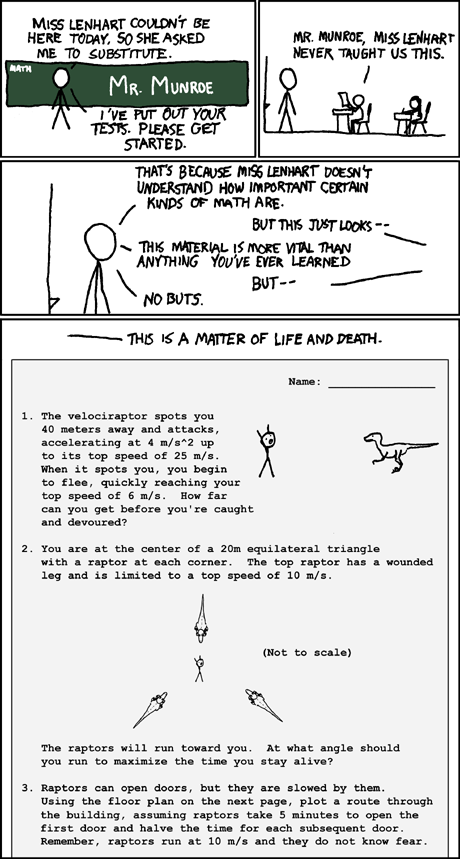
\includegraphics[width=0.7\hsize]{chapters/substitute.png}
\caption{xkcd 135 mit von Randall Munroe erdachten Aufgaben "uber die
Jagdgewohnheiten von Velociraptoren.
\label{einleitung:xkcd135}}
\end{figure}%


Das zweite Gesetz besagt:
\begin{quote}
\em
Die "Anderung der Bewegung ist der Einwirkung der bewegenden Kraft
proportional und geschieht nach der Richtung derjenigen geraden Linie,
nach welcher jene Kraft wirkt.
\end{quote}
Mit {\em Bewegung}
meint Newton den Impuls $\vec{p}=m\vec{v}$,
\index{Impuls}
das zweite Gesetz wird in moderner Schreibweise
\[
\frac{d}{dt}(m\vec{v}) = \vec{F}.
\]
In beiden F"allen wird die "Anderung einer Zustandsvariablen, n"amlich
des Impulses, mit dem aktuellen Zustand, typischerweise der Position,
verkn"upft.
Die Newtonsch-Bewegungsgesetze sind Differentialgleichungen.
\index{Newton!Bewegungsgesetz}

Das neue Werkzeug der Infinitesimalrechnung bescherte der exakten
Naturwissenschaft eine F"ulle neuer Probleml"osungen, die alle
nach dem gleichen Prinzip vorgingen.
Finde die Differentialgleichungen zwischen den Zustandsvariablen
eines Systems, "ublicherweise durch Anwendung des zweiten
Newtonschen Gesetztes, l"ose die Differentialgleichungen und
ziehe die Schl"usse.
Es zeigte sich jedoch bald, dass viele Differentialgleichungen
keine L"osungen haben, die sich mit den bisher bekannten Funktionen
ausdr"ucken lassen.
Man behalf sich kurzerhand damit, neue Funktionen zu definieren, 
die bald Anwendungen in den verschieden Gebieten der Technik fanden.
Die Bessel-Funktionen sind mittlerweile so wichtig, dass sie in keiner
Computer-Bibliothek f"ur mathematische Funktionen fehlen d"urfen.
\index{Bessel-Funktion}

Die Herkunft der Kr"afte wird in den Newtonschen Gesetzen nicht weiter
gekl"art, doch Newton selbst beschreibt mit seinem Gravitationsgesetz
die Herkunft der Kr"afte, die die Planeten im Sonnensystem auf ihren Bahnen
halten.
\index{Kepler!Johannes}
\index{Kepler-Bahn}
Er zeigt, dass die Keplerschen Ellipsenbahnen L"osungen seiner
Bewegungsgleichungen sind.
Die rein kinematische Beschreibung durch Kepler machte einem
dynamischen Verst"andnis Platz, welches nun auch die gegenseitigen
Einfl"usse der Planeten aufeinander zu berechnen gestattet.
Und tats"achlich war Newton der erste, der sich dar"uber Gedanken
machte, wie sich das Sonnensystem "uber lange Zeit entwickeln wird.
Seine Schlussfolgerung aus seinen aus heutiger Sicht rudiment"aren
Untersuchungen: das Sonnensystem ist instabil, "uber die Jahrmillionen 
werden die Planeten in den interstellaren Raum geschleudert werden.

Die industrielle Revolution brachte eine Vielzahl von Maschinen,
\index{industrielle Revolution}
die automatisch geregelt werden mussten.
Ingenieure entwickelten eine ganze Reihe von einfallsreichen L"osungen,
doch erst in der Mitte des 19.~Jahrhunderts konnten Physiker diese
Apparaturen mit Differentialgleichungen erkl"aren und ihre Stabilit"at
untersuchen.
Im zwanzigsten Jahrhundert reiften die mathematischen Hilfsmittel
soweit, dass auch instabile L"osungen untersucht werden konnten,
wie sie bei nichtlinearen Differentialgleichungen auftreten.
Mittlerweile ist das Auftreten Instabilit"aten recht gut verstanden
und klassifiziert. 
Die Technik der Linearisierung erm"oglicht zum Beispiel die
Hopf-Bifurkation zu verstehen.
\index{Hopf-Bifurkation}
\index{Bifurkation!Hopf}
Auch die Sattel-Knoten-Bifurkation und die Heugabel-Bifurkation
lassen sich in Anwendungen finden.
\index{Bifurkation!Sattel-Knoten-}
\index{Sattel-Knoten-Bifurkation}
\index{Bifurkation!Heugabel-}
\index{Heugabel-Bifurkation}
Und die Chaos-Theorie versteht sogar, wie "uber eine Kaskade von
Bifurkationen die Bewegung eines Systems jede Vorhersagbarkeit verliert,
es bewegt sich chaotisch.
\index{Chaos}

In vielen F"allen l"asst sich eine Differentialgleichung erst dann
verstehen, wenn man in komplexen Zahlen arbeiten. 
Die Hopf-Bifurkation tritt zum Beispiel genau dann auf, wenn eine
Bedingung "uber die Eigenwerte des linearisierten Systems erf"ullt ist.

Weitere Literaturhinweise im Literaturverzeichnis auf
Seite~\pageref{skript:literatur}.


%\input{kapitel.tex}
%
% grundlagen.tex -- Grundlagen ueber Differentialgleichungen
%
% (c) 2015 Prof Dr Andreas Mueller, Hochschule Rapperswil
%
\chapter{Grundlagen der Theorie der gew"ohnlichen Differentialgleichungen
\label{chapter:grundlagen}}
\lhead{}
\rhead{Grundlagen}
\section{Differentialgleichungen\label{section:differentialgleichungen}}
\lhead{Differentialgleichungen}
Eine gew"ohnliche Differentialgleichung f"ur eine reellwertige
Funktion $y(x)$ stellt einen Zusammenhang her zwischen der Funktion
und ihren Ableitungen.
Wir schreiben die Ableitungen als $y'$, $y''$, $y'''$ und $y^{(n)}$
f"ur die $n$-te Ableitung.
Wir lassen oft das Argument der Funktion weg.
Beispiele von Differentialgleichungen sind
\begin{align*}
y'&=-Ny
&&\text{Ordnung: $1$}
\\
y''&=-\omega^2 y
&&\text{Ordnung: $2$}
\\
x^2y''+xy'+(x^2-n^2)y&=0
&&\text{Ordnung: $2$}
\end{align*}
Die Abh"angigkeit kann in expliziter Form als
\begin{equation}
y^{(n)}=f(x,y,y',\dots,y^{(n-1)})
\label{grundlagen:explizit}
\end{equation}
oder in impliziter Form
\[
F(x,y,y',\dots,y^{(n)})=0
\]
gegeben sein.
Die Ordnung einer Differentialgleichung ist die h"ochste vorkommende
Ableitung.

\begin{figure}
\centering
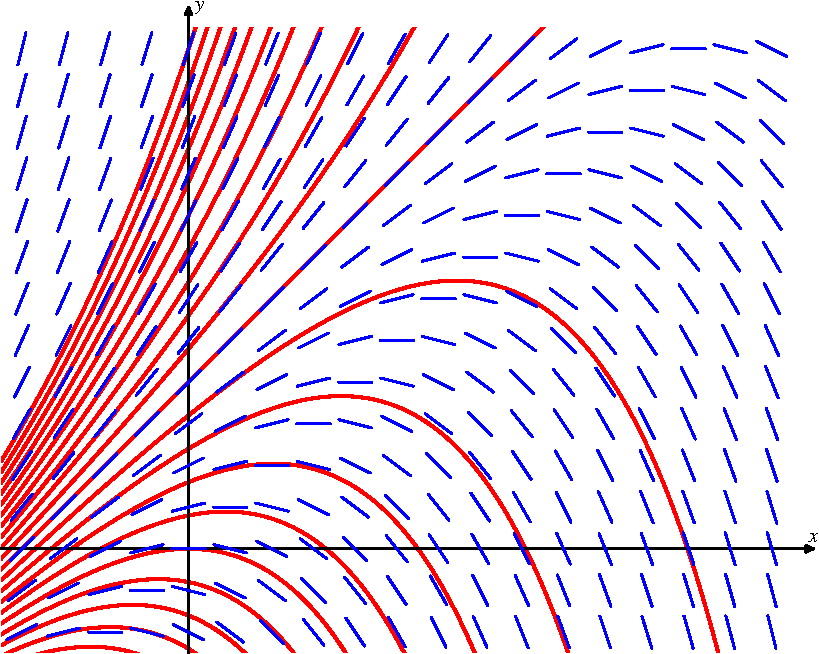
\includegraphics{chapters/images/grundlagen-1.pdf}
\caption{Richtungsfeld der Differentialgleichung $y'=y-x$ mit
einzelnen L"osungskurven.
\label{grundlagen:richtungsfeld}}
\end{figure}%

Differentialgleichungen erster Ordnung lassen sich mit Hilfe eines
Richtungsfeldes visualisieren, wie in Abbildung~\ref{grundlagen:richtungsfeld}
dargestellt.
In jedem Punkt $(x,y)$ der $x$-$y$-Ebene wird die Steigung $y'=f(x,y)$
eingezeichnet.
Eine L"osung der Differentialgleichung hat in diesem Bild als Graph
eine Kurve in der $x$-$y$-Ebene, die an jeder Stelle als Tangente 
das Richtungsfeld haben.

Insbesondere in Anwendungen in der Physik ist die Zeit die
unabh"angige Variable.
Die abh"angige Variable ist dann zum Beispiel die Ortskoordinate
$x(t)$ und wir bezeichnen ihre Ableitungen mit $\dot{x}(t)$ f"ur
die Geschwindigkeit, $\ddot{x}(t)$ f"ur die Beschleunigung.
Dieses Beispiel suggeriert auch, dass die abh"angige Variable 
ein Vektor sein kann, den man als den Ortsvektor eines Teilchens
interpretieren kann.
Auch die Funktion $f(t,x,\dots,x^{(n-1)})$ muss dann vektorwertig sein, und
ebenso alle Argumente ausser dem ersten von $f$.

Eine Differentialgleichung $n$-ter Ordnung f"ur eine skalare Funktion
kann in eine Vektor-Differen\-tialgleichung erster Ordnung f"ur eine
$n$-dimensionale vektorwertige Funktion umgewandelt werden.
Ist $y(x)$ die gesuchte Funktion in der
Differentialgleichung~(\ref{grundlagen:explizit}), dann kann man
den Vektor
\[
u(x)=\begin{pmatrix}
y(x)\\y'(x)\\\vdots\\y^{(n-1)}(x)
\end{pmatrix}
\in\mathbb R^n
\]
bilden.
Er erf"ullt die Differentialgleichung
\begin{equation}
\frac{d}{dx}\begin{pmatrix}
y\\y'\\\vdots\\y^{(n-1)}
\end{pmatrix}
=
\begin{pmatrix}
y'\\y''\\\vdots\\y^{(n)}
\end{pmatrix}
=
\begin{pmatrix}
y'\\y''\\\vdots\\f(x,y,y',\dots,y^{(n-1)})
\end{pmatrix}.
\label{grundlagen:vektordgl}
\end{equation}
Der Vektor auf der rechten Seite h"ang nur von $x$, der Funktion $y$
und ihren Ableitungen bis zur $n-1$-ten Ordnung ab, also von $u$, man
kann (\ref{grundlagen:vektordgl}) daher als
\begin{equation}
\frac{d}{dx}u=\tilde{f}(x,u)
\end{equation}
schreiben.
Im Folgenden werden wir fast ausschliesslich Differentialgleichungen
erster Ordnung der Form $y'=f(x,y)$ betrachten, und dabei stillschweigend
zulassen, dass $y$ ein Vektor ist.

Differentialgleichungen h"oherer Ordnung oder Vektordifferentialgleichungen
lassen sich nicht so einfach visualisieren wie Differentialgleichungen
erster Ordnung.
Ist $y(x)$ eine L"osung der Vektor-Differentialgleichung $y'=f(x,y)$
mit $y\in\mathbb R^n$, dann ist die Abbildung
\[
\gamma\colon
x\mapsto\begin{pmatrix}
x\\
y(x)
\end{pmatrix}\in\mathbb R^{n+1}
\]
eine Kurve im $n+1$-dimensionalen Raum. 
Der Tangentialvektor ist
\begin{equation}
\gamma'(x)
=
\begin{pmatrix}1\\y'(x)\end{pmatrix}
=
\begin{pmatrix}1\\f(x,y(x))\end{pmatrix}.
\label{grundlagen:gamma-vektorfeld}
\end{equation}
Die Kurve $\gamma(x)$ ist also in jedem Punkt des $n+1$-dimensionalen
Raumes tangential an das Vektorfeld, welches
durch~(\ref{grundlagen:gamma-vektorfeld}) definiert wird.
Der Spezialfall $n=1$ f"uhrt wieder zur"uck auf das Richtungsfeld
wie in Abbildung~\ref{grundlagen:richtungsfeld}.

\subsection{Anfangswertprobleme\label{section:anfangswertprobleme}}
Die Differentialgleichung $y'=f(x,y)$ alleine kann eine L"osungsfunktion
$y(x)$ nicht festlegen, sie codiert nur, wie sich die L"osung ver"andern wird.
Es ist also zus"atzlich die Angabe eines Punktes der L"osungskurve
notwendig.
Man nennt das Problem, eine Funktion $y(x)$ zu finden, welche
\[
y'=f(x,y)
\qquad
\text{und}
\qquad
y(0)=y_0
\]
erf"ullt, ein {\em Anfangswertproblem}.
Ein Anfangswertproblem verlangt f"ur die gew"ohnliche Differentialgleichung
$n$-ter Ordnung verlangt also die Angabe der Werte von
$y(0),y'(0),\dots,y^{(n-1)}(o)$

\subsubsection{Existenz und Eindeutigkeit von L"osungen}
Die Existenz und Eindeutigkeit einer L"osung ist aus den Beispielen und
graphischen Darstellungen intuitiv verst"andlich, f"ur einen exakten
Beweis sind jedoch zus"atzliche Voraussetzungen n"otig.

\begin{definition}
Eine Funktion $f\colon \mathbb R^n\to\mathbb R^m$ heisst global
{\em Lipschitz-stetig},
\index{Lipschitz-stetig}
wenn es eine Zahl $L$ gibt 
\begin{equation}
|f(x_2)-f(x_1)| \le L\,|x_2-x_1|
\label{grundlagen:lipschitz}
\end{equation}
f"ur alle Vektoren $x_1,x_2\in\mathbb R^n$.
Eine Funktion heisst lokal Lipschitz-stetig im Punkt $x_0$, wenn die
Bedingung (\ref{grundlagen:lipschitz}) f"ur $x_i$ in einer Umgebung von
$x_0$ erf"ullt ist.
\end{definition}

Eine Funktion ist insbesondere dann lokal Lipschitz-stetig, wenn sie
stetig differenzierbar ist.
In diesem Fall ist die Ableitung $f'(x)$ in einer Umgebung von $x_0$
beschr"ankt, also $|f(x)|<M$, und der Mittelwertsatz der Differentialgleichung
sagt, dass
\[
|f(x_2)-f(x_1)|\le M |x_2-x_2|
\]
ist, $f$ ist also lokal Lipschitz-stetig.

\begin{satz}[Picard-Lindel"of]
\label{grundlagen:picard-lindeloef}
Ist die Funktion $f(x,y)$ lokal Lipschitz-stetig bez"uglich der Variablen
$y$ f"ur $x\in[x_0,b]$ und $|y-y_0|<R$.
Dann hat das Anfangswertproblem
\[
y'(x)=f(x,y)\qquad\text{und}\qquad y(x_0)=y_0
\]
ein eindeutige L"osung, die in einem Interval $[x_0,x_0+\varepsilon)$
definiert ist.
\end{satz}

In diesem Buch werden die Funktionen $f$ der Differentialgleichungen 
meistens stetig differenzierbar sein, so dass der
Satz~\ref{grundlagen:picard-lindeloef} in unseren Anwendungen die lokale
Existenz und Eindeutigkeit einer L"osung garantiert.

\subsection{Autonome Differentialgleichungen}
Eine besondere Bedeutung haben Differentialgleichungen, in denen
$f$ nicht von $x$ abh"angt, man nennt sie {\em autonom}
\index{autonome Differentialgleichung}.
Die L"osungen einer solchen Differentialgleichungen h"angen im
folgenden Sinne nicht vom Start-$x$-Wert ab:
Ist $y(x)$ die L"osung des Anfangswertproblems
\[
y'=f(y)\qquad\text{und}\qquad y(0)=y_0,
\]
dann ist die Funktion
\[
y_1(x)=y(x-x_0)
\]
L"osung des Anfangswertproblems
\[
y'=f(y)\qquad\text{und}\qquad y(x_0)=y_0.
\]
Etwas salop kann man das auch so formulieren: f"ur den Verlauf der 
L"osungskurve kommt es nicht darauf an, wann die L"osungskurve bei 
einem Punkt vorbeikommt.
Der weitere Verlauf der L"osungskurve wird immer der gleiche sein,
unabh"angi davon, wann ein bestimmter Punkt besucht wird.

Die Darstellungen der L"osungskurven ohne die Angabe des
zugeh"origen $x$ sind daher f"ur autonome Differentialgleichungen
 aussagekr"aftig.
Wir nehmen im folgenden an, dass $f$ die Bedingungen f"ur Existenz
und Eindeutigkeit von L"osungen sowie f"ur die stetige Abh"angigkeit
von den Anfangsbedingungen erf"ullt.

\begin{figure}
\centering
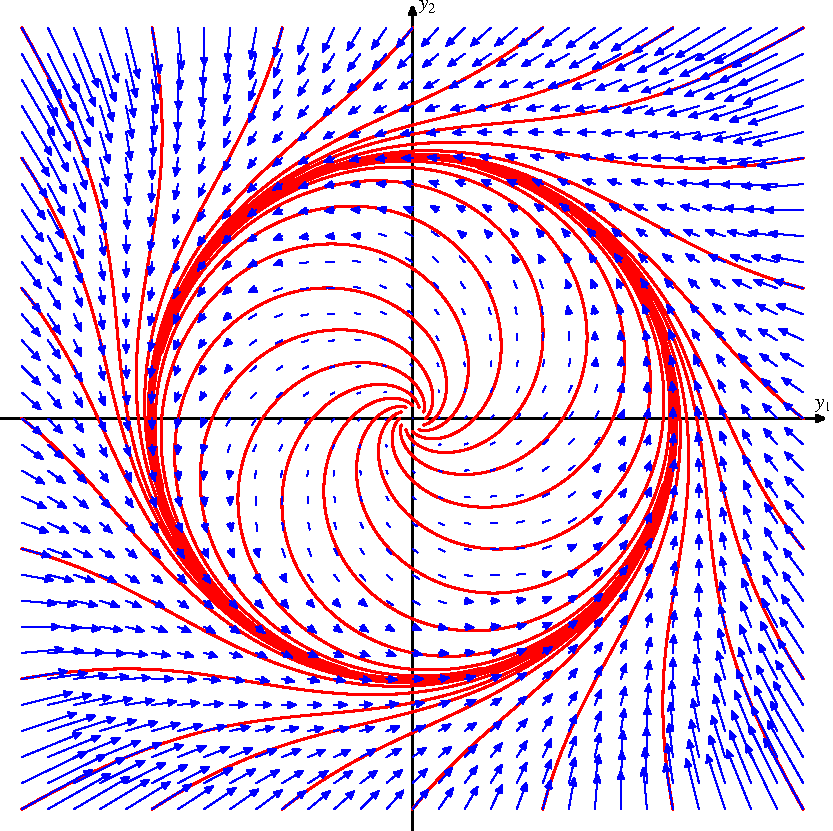
\includegraphics{chapters/images/grundlagen-2.pdf}
\caption{Vektorfeld des autonomen Differentialgleichungssystems
(\ref{grundlagen:hopfsystem})
mit L"osungskurven.
\label{grundlagen:vektorfeld}}
\end{figure}%

Eine autonome Differentialgleichung definiert in jedem Punkt des
Raumes, aus dem die $y$-Vektoren stammen, einen Vektor $f(y)$,
man spricht von einem {\em Vektorfeld}.
\index{Vektorfeld}
Indem wir in jedem Punkt des $y$-Raumes den Vektor $f(y)$ aufzeichnen,
k"onnen wir eine graphische Darstellung des Vektorfeldes erhalten
(Abbildung~\ref{grundlagen:vektorfeld}).
Die Bahn des Punktes $y(x)$ in Abh"angigkeit von $x$ ist eine Kurve,
deren Tangentialvektor in jedem Punkt der $y$-Ebene durch die Funktion
$f(y)$ gegeben ist.
In Abbildung~\ref{grundlagen:vektorfeld} ist das Vektorfeld des
Differentialgleichungssystems
\begin{equation}
\begin{aligned}
y_1'&=y_1-y_2-y_1(y_1^2+y_2^2)\\
y_2'&=y_1+y_2-y_2(y_1^2+y_2^2)
\end{aligned}
\label{grundlagen:hopfsystem}
\end{equation}
dargestellt.
Das Vektorfeld ist durch die Funktion $f(y)$ mit
\[
y=\begin{pmatrix}y_1\\y_2\end{pmatrix}
\qquad\text{und}\qquad
f(y)=\begin{pmatrix}
y_1-y_2-y_1(y_1^2+y_2^2)\\
y_1+y_2-y_2(y_1^2+y_2^2)
\end{pmatrix}
\]
gegeben.

Sehr viele Differentialgleichungen der Physik sind autonom.
Die unabh"angige Variable ist hier typischerweise die Zeit $t$, die
Naturgesetze, die Anlass zu den Differentialgleichungen geben,
h"angen nicht explizit von der Zeit ab. 
Zum Beispiel f"uhrt das Kraftgesetz der Gravitation auf die
Differentialgleichung
\[
m\ddot x=-\frac{GMm}{|x|^2}\frac{x}{|x|}
\]
f"ur die Bewegung eines Planeten der Masse $m$ um die Sonne mit Masse $M$.
Da die Massen konstant bleiben, tritt die Zeit auf der rechten Seite nicht
explizit auf.
Dies bedeutet auch, dass die Bahn immer gleich aussieht, unabh"angig
davon, wann der Planet startet.
In der Physik spricht man auch davon, dass die Bahn von einem 
Vektorfeld von Kraftvektoren $\vec F$ bestimmt wird.

F"ur eine autonome Differentialgleichung l"asst sich also zu jedem
Anfangspunkt eine L"osung finden.
Sind ausserdem die Voraussetzungen f"ur Existenz, Eindeutigkeit
und stetige Abh"angigkeit der L"osung von den Anfangsbedingungen erf"ullt,
k"onnen wir alle L"osungen in eine Funktion $\varphi$ zusammenfassen.
Sie ist definiert dadurch, dass
die Abbildung
\[
x\mapsto \varphi_x(y_0)
\]
L"osung des Anfangswertproblems
\[
y'=f(y)
\qquad\text{und}\qquad 
y(0)=y_0
\]
Wegen der Autonomie ist dann auch $y_{x-x_0}(y_0)$ L"osung des
Anfangswertproblems
\[
y'=f(y)
\qquad\text{und}\qquad 
y(x_0)=y_0,
\]
die Funktion $\varphi$ fasst also alle L"osungen in einer einzigen
Funktion zusammen.
Sie erf"ullt die Zusammensetzungsbedingung
\[
\varphi_{x_1+x_2}(y_0)=\varphi_{x_1}(\varphi_{x_2}(y_0)).
\]
Die Abbildung $\varphi$ heisst der {\em Fluss} des durch die autonome 
Differentialgleichung gegebenen Vektorfeldes.
\index{Fluss eines Vektorfeldes}

\subsubsection{Umwandlung in eine autonomes Problem}
Jede gew"ohnliche Differentialgleichung der Form
\begin{equation}
y'=f(x,y), \qquad y(0)=y_0
\label{skript:deautonom-dgl}
\end{equation}
kann in ein gleichbedeutendes autonomes Differentialgleichungssystem
umgewandelt werden.

Wir f"uhren zu diesem Zweck eine neue unabh"angige Variable $t$ ein,
und betrachten sowohl $x$ als auch $y$ als Funktionen von $t$. 
Die Funktion $f(x,y)$ h"angt nat"urlich nicht explizit von $t$ ab.
Die neue unabh"angige Variable soll sich nicht von $x$ unterscheiden,
wir fordern daher, dass $x$ die Differentialgleichung
\begin{equation}
\frac{dx}{dt}=1,\qquad x(0)=0
\label{skript:deautonom-param}
\end{equation}
erf"ullt ist, die wir sofort l"osen k"onnen: $x(t)=t$.
Wenn wir zur Differentialgleichung (\ref{skript:deautonom-dgl}) 
die Differentialgleichung (\ref{skript:deautonom-param}) hinzunehmen,
bekommen wir ein Differentialgleichungssystem, dessen rechte Seite
nicht explizit von  $t$ abh"angt.

Wir fassen $x$ und $y$ in einen $n+1$-dimensionalen Vektor $Y$ zusammen,
also
\[
Y
=
\begin{pmatrix}x\\y\end{pmatrix}
=
\begin{pmatrix}x\\y_1\\\vdots\\y_n\end{pmatrix}.
\]
Ausserdem schreiben wir
\[
F(Y)
=
\begin{pmatrix}1\\f(x,y)\end{pmatrix}
=
\begin{pmatrix}1\\f_1(x,y)\\\vdots\\f_n(x,y)\end{pmatrix},
\qquad
Y_0
=
\begin{pmatrix}0\\y_0\end{pmatrix}
=
\begin{pmatrix}0\\y_{0,1}\\\vdots\\y_{0,n}\end{pmatrix}.
\]
Mit dieser Notation ist das Differnialgleichungssystem
\[
\frac{d}{dt}Y=F(Y),\qquad Y(0)=Y_0
\]
ein autonomes System, welches die gleiche L"osung hat wie das
urspr"ungliche System.

\begin{satz}
Das $n$-dimensionale Differentialgleichungssystem 
\[
\frac{dy}{dx}=f(x,y)
\]
ist dem $n+1$-dimensionalen {\em autonomen} Differentialgleichungsssystem
\[
\frac{d}{dt}
\begin{pmatrix}
x\\y
\end{pmatrix}
=
\begin{pmatrix}1\\f(x,y)\end{pmatrix}
\]
"aquivalent.
\end{satz}

Die Tatsache, dass die Dimension des Systems erh"oht wird, hat tiefgreifende
Konsequenzen f"ur die m"oglichen L"osungen.
Zum Beispiel zeigt der Satz von Poincar\'e-Bendixson dass ein zweidimensionales
autonomes System keine chaotischen Bahnen haben kann.
Ein beliebiges eindimensionales System ist "aquivalent zu einem
zweidimensionalen autonomen System, also kann man in einem eindimensionalen
System kein chatoisches Verhalten beobachten.
Chaos verlangt nach einem autonomen System, welches mindestens dreidimensional
ist.
Oder einem beliebigen System mindestens von Dimension 2.

\subsection{Randwertprobleme\label{section:randwertprobleme}}
Wenn man einen Ball wirft, wird seine Bewegung durch die
Vektordifferentialgleichung zweiter Ordnung
\[
\frac{d^2}{dt^2}\begin{pmatrix}x\\y\end{pmatrix}
=
\begin{pmatrix}0\\\displaystyle-\frac{g}{m}\end{pmatrix}
\]
beschrieben.
Die Bahn ist ausserdem bestimmt durch die Anfangsbedingungen,
d.~h.~also den Anfangspunkt und die Anfangsgeschwindigkeit der Bahn.
Praktischer Ballwurf verlangt aber, dass ein Ziel erreicht wird.
Die Aufgabenstellung ist daher eine Bahnkurve $\gamma(t)$ zu finden,
welche sowohl durch den Anfangspunkt als auch den Zielpunkt
verl"auft.

Die L"osung einer Differentialgleichungen erster Ordnung f"ur eine
unbekannte reellwertige Funktion $y(x)$ ist vollst"andig durch einen
einzigen Anfangswert bestimmt.
Eine Differentialgleichung zweiter Ordnung f"ur eine unbekannte
rellwertige Funktion $y(x)$ verlangt dagegen zwei Anfangswerte,
n"amlich f"ur $y(0)$ und $y'(0)$.
In Analogie zum Problem des Ballwurfs k"onnte die L"osungsfunktion auch
festgelegt werden durch den Wert f"ur $x=0$ und $x=1$.
Gesucht ist also eine Funktion $y(x)$ auf dem Interval $[0,1]$, die
\begin{equation}
y''=f(x,y,y')
\qquad\text{mit}\qquad
y(0)=y_0,
\qquad
y(1)=y_1
\end{equation}
erf"ullt.

\begin{beispiel}
Wir l"osen die Differentialgleichung $y''=-y$ mit den Randwerten
$y(0)=1$ und $y(1)=2$.
Die homogene Differentialgleichung hat die Funktionen
\[
y(x)=A \cos x + B\sin x
\]
als allgemeine L"osung.
Die Konstanten $A$ und $B$ m"ussen so gew"ahlt werden, dass die Randwerte
korrekt sind.
Setzt man $x=0$ und $x=1$ ein, erh"alt man die linearen Gleichungen
\begin{align*}
a=y(0)&=A\cos 0 + B\sin 0=A\\
b=y(1)&=A\cos 1 + B\sin 1
\qquad\Rightarrow\qquad
\frac{b-a\cos 1}{\sin 1}.
\end{align*}
Die L"osung des Randwertproblems ist daher die Funktion
\[
y(x)=a\cos x +\frac{b-a\cos 1}{\sin 1}\sin x,
\]
wie man auch durch Einsetzen von $x=0$ und $x=1$ verifizieren kann.
\end{beispiel}

\subsection{H"ohere Ableitungen\label{grundlagen:hoehere-ableitungen}}
Die Differentialgleichung $y'=f(x,y)$ erlaubt nicht nur die erste
Ableitung einer Funktion zu bestimmen.
Durch Ableitung nach $x$ k"onnen wir auch die h"oheren Ableitungen
bestimmen, die eine L"osung der Differentialgleichung haben muss,
die durch den Punkt $(x,y)$.
\begin{align}
y'(x)
&=
f(x,y),
\notag
\\
y''(x)
&=
\frac{dy'(x)}{dx}
=
\frac{\partial f(x,y)}{\partial x} + \frac{\partial f(x,y)}{\partial y}y'(x)
=
\frac{\partial f(x,y)}{\partial x} + \frac{\partial f(x,y)}{\partial y}f(x,y),
\label{grundlagen:2abl}
\\
y'''(x)
&=
\frac{dy''(x)}{dx}
\notag
\\
&=
\frac{\partial^2 f(x,y)}{\partial x^2}
+ \frac{\partial^2 f(x,y)}{\partial y\,\partial x}y'(x)
+ \biggl(\frac{\partial^2 f(x,y)}{\partial x\,\partial y}
+ \frac{\partial^2 f(x,y)}{\partial y^2}y'(x)\biggr)f(x,y)
\notag
\\
&\qquad
+ \frac{\partial f(x,y)}{\partial y}\biggl(
\frac{\partial f(x,y)}{\partial x} + \frac{\partial f(x,y)}{\partial y}f(x,y)
\biggr),
\notag
\\
&=
\frac{\partial^2 f(x,y)}{\partial x^2}
+ 2\frac{\partial^2 f(x,y)}{\partial x\,\partial y}f(x,y)
+ \frac{\partial^2 f(x,y)}{\partial y^2}f(x,y)^2
+ \biggl(\frac{\partial f(x,y)}{\partial y}\biggr)^2 f(x,y)
+ \frac{\partial f(x,y)}{\partial y} \frac{\partial f(x,y)}{\partial x}.
\label{grundlagen:3abl}
\end{align}
Die Terme werden offensichtlich schnell kompliziert.

\subsection{Ableitung nach der Anfangsbedingung}
Ver"andert man die Anfangsbedingung, "andert sich auch die L"osung,
die Komponentent $y_i$ ist also eine Funktion von $x$ und
von allen Anfangswerten $y_{j0}$:
\[
y_i(x, y_{10},\dots,y_{n0}).
\]
Wenn man untersuchen will, wie empfindlich die $y_i$ auf "Anderungen
der Anfangswerte reagieren, dann sucht man die Ableitungen der $y_i$
nach den Anfangswerten, also die sogenannte Jacobi-Matrix
\[
J(x)
=
\begin{pmatrix}
\displaystyle\frac{\partial y_1}{\partial y_{10}}&\dots&
	\displaystyle\frac{\partial y_1}{\partial y_{n0}}\\
\vdots&\ddots&\vdots\\
\displaystyle\frac{\partial y_n}{\partial y_{10}}&\dots&
	\displaystyle\frac{\partial y_n}{\partial y_{n0}}\\
\end{pmatrix}
\]
Wir schreiben abk"urzend auch 
\[
J(x)= \frac{\partial y}{\partial y_0}.
\]
F"ur $x=0$ ist $y(x)=y(0)=y_0$, die Ableitung der $y$-Werte nach den
Anfangswerten ist daher die Einheitsmatrix:
\[
J(0)=E,
\]
und es liegt nahe, dass auch $J(x)$ eine Differentialgleichung erf"ullen
muss.

Wie "andert sich $J(x)$ zwischen $x$ und $x+\Delta x$?
Die Werte von $y$ "andern sich um
\begin{equation}
\frac{dy}{dx}= f(x,y),
\label{grundlagen:jacobi-1}
\end{equation}
aber $y$ h"angt von den Anfangsbedingungen ab.
Leiten wir (\ref{grundlagen:jacobi-1}) nach $y_0$ ab, finden wir
\begin{equation}
\frac{\partial}{\partial y_0}\frac{dy}{dx}
=
\frac{\partial}{\partial y_0}f(x,y).
\label{grundlagen:jacobi-2}
\end{equation}
Die rechte Seite wir mit der Kettenregel zu
\begin{align*}
\frac{\partial}{\partial y_{j0}}f_i(x,y).
&=
\sum_{k=1}^n \frac{\partial f_i(x,y)}{\partial y_{k}}
\underbrace{\frac{\partial y_k}{\partial y_{j0}}}_{J_{ij}(x)}.
\end{align*}
Schreiben wir die Ableitungen von $f$ nach $y$ in die Matrix
\[
\frac{\partial f(x,y)}{\partial y}
=
\begin{pmatrix}
\displaystyle\frac{\partial f_1(x,y)}{\partial y_1}&\dots&
	\displaystyle\frac{\partial f_1(x,y)}{\partial y_n}\\
\vdots&\ddots&\vdots\\
\displaystyle\frac{\partial f_n(x,y)}{\partial y_1}&\dots&
	\displaystyle\frac{\partial f_n(x,y)}{\partial y_n}
\end{pmatrix}
=F(x,y),
\]
kann die Gleichung (\ref{grundlagen:jacobi-2}) mit dem Matrizenprodukt als
\begin{equation*}
\frac{\partial}{\partial y_0}\frac{dy}{dx}
=
F(x,y)J(x)
\end{equation*}
sehr viel kompakter geschrieben werden.
Die Ableitungen auf der linken Seite vertauschen, und wir erhalten

\begin{satz}
Ist $y(x,y_0)$ die L"osung der Differentialgleichung 
\[
y'=f(x,y)\qquad\text{mit Anfangsbedingung}\qquad y(0)=y_0,
\]
dann erf"ullt die Jacobi-Matrix 
\[
\frac{\partial y}{\partial y_0}=J(x)
\]
die Differentialgleichung
\begin{equation}
\frac{d}{dx}\frac{\partial y}{\partial x}
=
\frac{d}{dx}J(x)
=
F(x,y)J(x)
\qquad
\text{mit Anfangsbedingung}
\qquad
J(x)=E.
\label{grundlagen:jacobi-dgl}
\end{equation}
wobei $F$ die Ableitung von $F$ nach $y$ ist,
\[
F(x,y)=\frac{\partial f(x,y)}{\partial y}.
\]
\end{satz}
Vor allem bei der numerischen L"osung mit dem Computer l"asst sich
die Jacobi-Matrix also gleich mit bestimmen, indem man die gefundene
L"osung $y$ als Input f"ur die Gleichung (\ref{grundlagen:jacobi-dgl})
verwendet.

\begin{beispiel}
Wir betrachten wieder die Schwingungsdifferentialgleichung $y''=-y$,
oder vielmehr die Form erster Ordnung
\[
\frac{d}{dx}\begin{pmatrix}y_1\\y_2\end{pmatrix}
=
\begin{pmatrix}
y_2\\-y_1.
\end{pmatrix}.
\]
Die Ableitungsmatrix $F(x,y)$ ist
\[
F(x,y)
=
\begin{pmatrix}
\displaystyle\frac{\partial f_1}{\partial y_1}&\displaystyle\frac{\partial f_1}{\partial y_2}\\
\displaystyle\frac{\partial f_2}{\partial y_1}&\displaystyle\frac{\partial f_2}{\partial y_2}
\end{pmatrix}
=
\begin{pmatrix}
 0&1\\
-1&0
\end{pmatrix}
\]
Die Jacobi-Matrix erf"ullt also die Differentialgleichung
\[
\frac{d}{dx}J(x)=\begin{pmatrix}0&1\\-1&0\end{pmatrix}J(x).
\]
Da wir die Differentialgleichung bereits vollst"andig gel"ost und
die L"osung
\[
\begin{pmatrix}
y_1(x)\\y_2(x)
\end{pmatrix}
=
\begin{pmatrix}
 y_{10}\cos x+y_{20}\sin x\\
-y_{10}\sin x+y_{20}\cos x
\end{pmatrix}
=
\begin{pmatrix}
 \cos x&\sin x\\
-\sin x&\cos x
\end{pmatrix}
\begin{pmatrix}y_{10}\\y_{20}\end{pmatrix}
\]
gefunden haben, k"onnen wir die Jacobi-Matrix auch aus der L"osung berechnen,
und verifizieren, ob sie die Differentialgleichung erf"ullt.
Die Jacobi-Matrix ist
\begin{align*}
J(x)
=
\frac{\partial y}{\partial y_0}
&=
\begin{pmatrix}
 \cos x&\sin x\\
-\sin x&\cos x
\end{pmatrix}
\end{align*}
Die Ableitung davon ist
\[
\frac{d}{dx}J(x)
=
\begin{pmatrix}
-\sin x& \cos x\\
-\cos x&-\sin x
\end{pmatrix}
\]
Setzen wir dies in die Differentialgleichung (\ref{grundlagen:jacobi-dgl}) ein
finden wir
\[
F(x,y)J(x)
=
\begin{pmatrix}
 0&1\\
-1&0
\end{pmatrix}
\begin{pmatrix}
 \cos x&\sin x\\
-\sin x&\cos x
\end{pmatrix}
=
\begin{pmatrix}
-\sin x& \cos x
-\cos x&-\sin x\\
\end{pmatrix}
=
\frac{d}{dx}J(x),
\]
die Differentialgleichung ist also tats"achlich erf"ullt.
\end{beispiel}
Die M"oglichkeit, die Jacobi-Matrix zu berechnen, wird sich im
Abschnitt~\ref{numerik:schiess-verfahren} bei der numerischen
L"osung von Randwertproblemen als besonders n"utzlich erweisen.

\section{Analytische L"osungsverfahren\label{section:analytischeverfahren}}
\lhead{Analytische L"osungsverfahren}
Nur wenige Differentialgleichungen lassen sich in geschlossener Form
l"osen, weshalb wird in Kapitel~\ref{chapter:numerik} Methoden zur
numerischen L"osung studieren werden.
In einzelnen F"allen lassen sich jedoch L"osungsverfahren angeben,
mit denen man Formeln f"ur die L"osungen finden kann.
Einige davon sollen in diesem Abschnitt kurz zusammengestellt werden.

\subsection{Separierbare Differentialgleichungen}
Differentialgleichungen erster Ordnung lassen sich oft durch sogenannte
Trennung der Variablen auf die Berechnung von Integralen reduzieren.
Dank der Schreibweise der Ableitung als Differentialquotient wird
dieser L"osungsweg sehr suggestiv.
Wir betrachten als Beispiel die Differentialgleichung
\[
y'=-Ny.
\]
Schreibt man die Ableitung als Differentialquotient, wird daraus die
Gleichung
\[
\frac{dy}{dx}=-Ny.
\]
Durch Division durch $y$ und formale Multiplikation mit $dx$ wird daraus
die formale Gleichung
\begin{equation}
\frac{dy}{y}=-N\,dx.
\label{grundlagen:separiert}
\end{equation}
In dieser Gleichung kommt die Variable $y$ nur auf der linken, die Variable
$x$ nur auf der rechten Seite vor.
Man sagt, die Variablen seien {\em separiert}.
\index{separiert}
\index{Variablen, Separation der}
Man beachte, dass die Gleichung (\ref{grundlagen:separiert}) nur eine
formale Bedeutung haben kann, die Symbole $dy$ und $dx$ sind ja keine Zahlen,
mit denen man algebraische Operationen durchf"uhren k"onnte.
Mit etwas Vorsicht angewandt f"uhrt dieser Kalk"ul aber nicht auf
Widerspr"uche.

Wir integrieren jetzt beide Seiten von (\ref{grundlagen:separiert}), und
erhalten 
\[
\int\frac1y\,dy=-N\int\,dx
\]
Beide Integrale lassen sich in geschlossener Form auswerten:
\[
\log|y|=-Nx+C.
\]
Aufgel"ost nach $y$ ergibt sich
\[
y=\pm e^{C}e^{-Nx},
\]
wobei die beiden Vorzeichen $\pm$ das Betragszeichen in der Stammfunktion
von $\frac1y$ reflektieren.
Man kann den Faktor $\pm e^{C}$ in eine neue Konstante $a$ zusammenfassen,
und erh"alt somit als L"osung der urspr"unglichen Differentialgleichung
die Familie
\[
y(x)=ae^{-Nx}
\]
von Funktionen.
Der Paramter $a$ muss mit Hilfe der Anfangsbedingung festgelegt werden.

Etwas allgemeiner kann die Methode der Separation der Variablen wie folgt
formuliert werden:
\begin{definition}
\label{grundlagen:definition:separierbar}
Eine Differentialgleichung der Form
\[
y'=f(y) g(x)
\]
mit stetigen Funktionen $f(y)$ und $g(x)$ heisst separierbar.
\end{definition}

\begin{satz}[Separation der Variablen]
Eine separierbare Differentialgliechung mit Funktionen $f$ und $g$ wie
in Definition~\ref{grundlagen:definition:separierbar},
die ausserdem in einer Umgebung von $x_0$ und $y_0$ nicht verschwinden.
Ausserdem sollen
\[
F(y)=\int_{y_0}^y \frac1{f(\eta)}\,d\eta
\qquad\text{und}\qquad
G(x)=\int_{x_0}^x g(\xi)\,d\xi
\]
Stammfunktionen sein.
Dann ist $F$ in einer Umgebung von $y_0$ invertierbar und es gilt
\[
y(x)=F^{-1}(G(x))
\]
\end{satz}

\begin{proof}[Beweis]
Sei $y(x)$ die L"osung der Differentialgleichung, die die Anfangsbedinung
$y(x_0)=y_0$ erf"ullt.
Wir setzen $y(x)$ in die Differentialgleichung ein,
dividieren sie durch $f(y)$ und integrieren "uber $x$:
\[
\int_{x_0}^x\frac1{f(y(\xi))}\frac{dy(\xi)}{d\xi}\,d\xi
=
\int_{x_0}^x g(\xi)\,d\xi.
\]
Die linke Seite kann mit der Formel f"ur die Variablentransformation in
ein Integral "uber $y$ umgewandelt werden.
\[
\int_{x_0}^x\frac1{f(y(\xi))}\frac{dy(\xi)}{d\xi}\,d\xi
=
\int_{y_0}^y \frac1{f(\eta)}\,d\eta=F(y)
\]
die L"osung muss daher die Gleichung
\begin{equation}
F(y(x))=G(x)
\label{grundlagen:FG}
\end{equation}
erf"ullen.
Da $f(y)\ne 0$ in einer Umgebung von $y_0$, ist $F$ in einer Umgebung von $y_0$
streng monoton wachsend oder fallend und damit invertierbar.
Also ist die Gleichung~(\ref{grundlagen:FG}) nach $y(x)$ aufl"osbar, und
es gilt
\[
y(x)=F^{-1}(G(x)).
\]
\end{proof}

\begin{beispiel}
Als Beispiel l"osen wir die Differentialgleichung
\[
y'=\frac{y^2+1}{x^2-1}
\]
mit den Anfangsbedingungen $x_0=0$ und $y(x_0)=y(0)=1$.
Die Differentialgleichung ist separierbar, die beiden Funktionen sind
\begin{align*}
f(y)&=y^2+1
\\
g(x)&=\frac1{x^2-1}.
\end{align*}
Wir brauchen die beiden Stammfunktionen $F(y)$ und $G(x)$:
\begin{align*}
F(y)
&=
\int_{y_0}^y \frac1{f(\eta)}\,d\eta
=
\int_{1}^y \frac1{\eta^2+1}\,d\eta
=
\arctan y - \frac{\pi}2,
\\
G(x)
&=
\int_{x_0}^x\frac1{\xi^2-1}\,d\xi
=
\int_0^x \frac1{\xi^2-1}\,d\xi
=
\frac12(\log(1-x)-\log(1+x)).
\end{align*}
Die Umkehrfunktion von $F$ ist
\[
F^{-1}(u)=\tan\biggl(u+\frac{\pi}2\biggr),
\]
so dass die L"osung der Differentialgleichung
\[
y(x)=
\tan\biggl(\frac12\log(1-x)-\frac12\log(1+x)+\frac{\pi}2\biggr)
\]
ist.
Tats"achlich "uberpr"uft man leicht, dass $y(0)=\tan\frac{\pi}2=1$ ist.
\end{beispiel}

\subsection{Lineare Differentialgleichungen}
Eine Differentialgleichung der Form
\begin{equation}
a_n(x)y^{(n)}+a_{n-1}(x)y^{(n-1)}+\dots+a_2(x)y''+a_1(x)y'+a_0(x)=f(x)
\label{grundlagen:linearedgl}
\end{equation}
heisst {\em lineare Differentialgleichung}.
\index{lineare Differentialgleichung}
Ist $f(x)=0$, nennt man die Differentialgleichung {\em homogen}, die
Funktion $f(x)$ wird auch die {\em Inhomogenit"at} genannt.
\index{homogen Differentialgleichung}
\index{Inhomogenitat@Inhomogenit\"at}
Die L"osungsmenge einer homogenen linearen Differentialgleichung
bildet einen Vektorraum: jede Linearkombination von L"osungen
ist wieder eine L"osung.
Seien zum Beispiel $y_1(x)$ und $y_2(x)$ L"osungen der Differentialgleichung
(\ref{grundlagen:linearedgl}).
Wir m"ochten zeigen, dass
$y(x)=\alpha y_1(x)+\beta y_2(x)$ eine L"osung ist.
Die Ableitungen selbst sind linear:
\begin{align*}
y^{(k)}(x)&=\alpha y_1^{(k)}(x)+\beta y_2^{(k)}(x).
\end{align*}
Setzt man dies in die Differentialgleichung ein, erh"alt man
\begin{align*}
a_ny^{(n)}+\dots+a_1y'+a_0y
&=
a_n\alpha y_1^{(n)}+a_n\beta y_2^{(n)}+\dots+a_1\alpha y_1'+a_1\beta y_2'
+ a_0\alpha y_1+a_0\beta y_2
\\
&=
\alpha(\underbrace{a_ny_1^{(n)}+\dots+a_1y_1'+a_0y_1}_{=0})
+
\beta(\underbrace{a_ny_2^{(n)}+\dots+a_1y_2'+a_0y_2}_{=0})=0,
\end{align*}
die Linearkombination $y$ erf"ullt also die homogene Differentialgleichung
ebenfalls.

Sind $y_1$ und $y_2$ zwei verschiedene L"osungen der inhomogenen
Differentialgleichung, dann gilt f"ur deren Differenz
\[
a_n(x)(y^{(n)}_1(x)-y^{(n)}_w(x))+\dots+a_1(x)(y_1'(x)-y_2'(x))+a_0(x)(y_1(x)-y_2(x))=f(x)-f(x)=0,
\]
also ist $y_1(x)-y_2(x)$ eine L"osung der homogenen Differentialgleichung.
Jeder L"osung der inhomogenen Differentialgleichung kann daher aus einer
einzigen L"osung der inhomogenenen Gleichung gewonnen werden, indem man
eine L"osung er homogenen Differentialgleichung addiert.

\begin{satz}
Die L"osungsmenge der  inhomogene lineare Differentialgleichung
(\ref{grundlagen:linearedgl}) ist
\[
{\mathbb L}=\{
y_p(x)+y_h(x)\;|\; y_h(x)=\mathbb L_h
\},
\]
wobei $\mathbb L_h$ die L"osungsmenge der zugeh"origen homogenen
Gleichung ist.
$y_p(x)$ heisst {\em partikul"are L"osung} der inhomogenen Gleichung.
\end{satz}
\index{partiklare Losung@partikul\"are L\"osung}

\subsection{Konstante Koeffizienten}
Im Spezialfall konstanter Koeffizienten l"asst sich die homogene
Differentialgleichung
\begin{equation}
a_ny^{(n)}+a_{n-1}y^{(n-1)}+\dots+a_2y''+a_1y'+a_0=0
\label{grundlagen:homogenedgl}
\end{equation}
mit Hilfe eines Exponentialansatzes l"osen.
Dazu setzt man 
\[
y(x)=e^{\lambda x}
\]
an, und setzt dies in die Differentialgleichung ein.
Man erh"alt
\[
(a_n\lambda^n a_{n-1}\lambda^{n-1}+\dots+a_2\lambda^2+a_1\lambda+a_0)e^{\lambda x}=0
\]
Da $e^{\lambda x}\ne 0$ ist, kann man diesen Faktor wegk"urzen und erh"alt
als Bedingung an $\lambda$ die Gleichung
\[
a_n\lambda^n a_{n-1}\lambda^{n-1}+\dots+a_2\lambda^2+a_1\lambda+a_0=0.
\]
Die in Frage kommenden $\lambda$ m"ussen also Nullstellen des Polynoms
mit Koeffizienten $a_i$ sein:

\begin{definition}
Die lineare homogene Differentialgleichung mit Konstanten Koeffizienten
(\ref{grundlagen:homogenedgl}) hat das {\em charakteristische Polynome}
\begin{equation}
\chi(\lambda)
=
a_n\lambda^n a_{n-1}\lambda^{n-1}+\dots+a_2\lambda^2+a_1\lambda+a_0
\end{equation}
Die Gleichung $\chi(\lambda)=0$ heisst die charakteristische Gleichung
der Differentialgleichung.
\end{definition}

\begin{satz}
Sind $\lambda_i$ die Nullstellen des charakteristischen Polynoms der
lineare homogenen Differentialgleichung mit konstanten Koeffizienten
(\ref{grundlagen:homogenedgl}), dann sind die Funktionen
$y_i(x)=e^{\lambda_i x}$ L"osungen.
Ist $\lambda$ eine $k$-fache Nullstelle, dann sind ausserdem die
Funktionen
\[
xe^{\lambda x},\quad x^2e^{\lambda x},\quad\dots\quad x^{k-1}e^{\lambda x}
\]
L"osungen.
\end{satz}

%
% XXX Begr"undung im Kapitel über Matrix-Differentialgleichungen 
%

\subsection{Variation der Konstanten}
Die allgemeine L"osung einer inhomogenen linearen Differentialgleichung ist die
Summe aus einer einzigen L"osung der inhomogenen Gleichung und einer
beliebigen L"osung der homogenen Gleichung.
Die L"osungen der homogenen Gleichung k"onnen mit Hilfe des charakteristischen
Polynoms bestimmt werden, doch wie findet man partikul"are L"osungen?
Auf der rechten Seite kann eine beliebige Funktion stehen, es ist also
ein wesentlich vielf"altigere L"osungsmenge zu erwarten.

\subsubsection{Motivation}
Betrachten wir als Motivationsbeispiel eine Schwingungsdifferentialgleichung
\[
y''+y=f.
\]
Die homogene Gleichung hat zwei L"osungen $y_1(x)=\cos x$ und $y_2(x)=\sin x$,
die allgemeine L"osung ist eine Linearkombination 
\[
y(x)=A_1y_1(x)+A_2y_2(x).
\]
Die Koeffizienten $A_1$ und $A_2$ haben die Bedeutung der Amplitude er
beiden Komponenten $y_1(x)$ und $y_2(x)$.

Die Inhomogenit"at $f(x)$ auf der rechten Seite steuert das Verhalten
der Differentialgleichung, moduliert also die Schwingung.
Wir erwarten daher, dass sich die L"osung der inhomogenen Gleichung
aus den L"osungen der homogenen Differentialgleichung dadurch gewinnen
l"asst, dass man die Amplituden von $x$ abh"angig macht.
Wir erwarten daher die partikul"are L"osung in der Form
\[
y_p(x)=A_1(x)y_1(x)+A_2y_2(x)
\]
mit noch zu bestimmenden Funktionen $A_1(x)$ und $A_2(x)$.
In den folgenden Rechnungen lassen wir das Argument der K"urze und Lesbarkeit
halber wieder weg.
F"ur die Ableitungen erhalten wir:
\begin{align*}
y_p'
&=
A_1'y_1+A_1y_1'+A_2'y_2+A_2y_2'
\\
y_p''
&=
A_1''y_1+2A_1'y_1'+A_1y_1''+2A_2'y_2'+A_2''y_2+A_2y_2''
\\
y_p''-y_p
&=
A_1''y_1+2A_1'y_1'+A_1(\underbrace{y_1''+y_1}_{=0})
+
A_2''y_2+2A_2'y_2'+A_2(\underbrace{y_2''+y_2}_{=0})
\end{align*}
Setzen wir dies in die Differentialgleichung ein erhalten wir die
lineare Differentialgleichung 
\[
A_1''y_1+2A_1'y_1' +A_2''y_2+2A_2'y_2'=f
\]
erster Ordnung f"ur die Funktionen $A_1'$ und $A_2'$.
F"ur die oben gefundenen Funktionen ist $y_1'=-\sin x$, $y_2'=\cos x$,
die Differentialgleichung wird damit zu
\[
A_1''\cos x -2A_1'\sin x +A_2''\sin x+2A_2'\cos x=f.
\]
Diese Differentialgleichung ist zwar immer noch inhomogen, aber sie
ist niedrigerer Ordnung.
Leider suchen wir jetzt auch zwei Funktionen, aber das r"uhrt daher, dass
wir nicht alle Information ausgenutzt haben.

Man nennt das angedeutete Verfahren {\em Variation der Konstanten}.
Um aus dieser Idee ein brauchbares Verfahren zu machen, entwickeln wir es
in den n"achsten Unterabschnitten systematisch, beginnend mit der Fall
einer Differentialgleichung erster Ordnung.

\subsubsection{Variation der Konstanten, 1.~Ordnung, $n=1$}
Wir gehen aus von einer linearen Differentialgleichung erster Ordnung,
also einer Gleichung der Form
\[
y' + a(x)y=f(x),
\]
und nehmen an, dass die allgemeine L"osung der homogenen Gleichung
durch die Funktion $y_h(x)$ gegeben ist.

Gem"ass der oben skizzierten Idee setzen wir jetzt f"ur die partikl"are
L"osung 
\[
y_p(x)=A(x) y_1(x)
\]
an, und setzen dies in die Differentialgleichung
\begin{align*}
y_p'(x)
&=
A'(x)y_h(x)+A(x)y_h'(x)
\\
y_p'+a(x)y_p(x)
&=
A'(x)y_h(x)+A(x)y_h'(x)
+
a(x)A(x)y_1(x)
\\
&=
A'(x)y_h(x)+A(x)(\underbrace{y_h'(x)+a(x)y_h'(x)}_{=0})=f
\end{align*}
Damit haben wir eine Differentialgleichung f"ur $A'(x)$ gefunden.
Als Anfangsbedingung m"ussen wir $A(0)$ so w"ahlen, dass
die Anfangsbedingung erf"ullt ist:
\[
y(0)=y_0
\qquad\Rightarrow\qquad
A(0)y_h(0)=y_0
\qquad\Rightarrow\qquad
A_0=A(0)=\frac{y_0}{y_h(0)}.
\]
Die Differentialgleichung l"asst sich mit einer Integration l"osen:
\begin{align*}
A'(x)
&=
f(x)/y_h(x)
\\
\Rightarrow\qquad
A(x)
&=
A_0+
\int_0^x \frac{f(x) }{y_h(x)}\,dx.
\end{align*}
Damit k"onnen wir eine Formel f"ur $y_p(x)$ angeben.

\begin{satz}
Wenn die homogene Differentialgleichung
\[
y'(x)+a(x)y(x) = 0
\]
die L"osung $y_h(x)$ hat, dann ist
\[
y_p(x)=y_0+\int_0^x\frac{f(\xi)}{y_h(\xi)}\,d\xi\cdot y_h(x)
\]
mit eine partiklu"are der inhomogenen Gleichung
\[
y'(x)+a(x)y(x)=f(x)
\]
und der Anfangsbedingung $y(0)=y_0$.
\end{satz}

\begin{beispiel}
In diesem Beispiel m"ochten wir zeigen, dass die Idee der Modulation,
mit der das Verfahren motiviert worden war, tats"achlich funktioniert.
Wir verwenden dazu die komplexe Differentialgleichung
\[
y'+iy=\sin \omega x,
\]
wobei $\omega \ll 1$ sein soll.
Die homogene Differentialgleichung hat die L"osung $y_h(x)=e^{-ix}$,
also eine (komplexe) Schwingung.
Nach der eben entwickelten Theorie muss eine partikul"are L"osung
mit Hilfe des Ausdrucks
\[
y_p(x)=y_0 +\int_0^x\frac{\sin\omega\xi}{e^{-i\xi}}\,d\xi\cdot e^{-ix}
\]
gefunden werden k"onnen.
Das Integral l"asst sich in geschlossener Form auswerten:
\begin{align*}
y_p(x)
&=
y_0 + \int_0^x \sin\omega\xi e^{i\xi}\,d\xi\cdot e^{-ix}
\\
&=
y_0+
\frac{i\sin \omega x- \omega \cos \omega x}{\omega^2-1}
+\frac{\omega}{\omega^2-1}e^{-ix}
\end{align*}
\end{beispiel}

\subsubsection{Variation der Konstanten, 1.~Ordnung, $n$ beliebig}
Eine $n$-dimensionale lineare Differentialgleichung 1.~Ordnung ist
eine Gleichung der Form
\[
\frac{dy}{dx}+f(x)\cdot y = g
\]
wobei $f(x)$ f"ur jedes $x$ ein $n\times n$-Matrix ist.
Wir nehmen wieder an, dass wir $n$ linear unabh"angige L"osungen
$y_1,\dots,y_n$ der homogenen Gleichung
\[
\frac{dy}{dx}+f(x)\cdot y=0
\]
bereits gefunden haben.
Wir suchen Koeffizienten $A_1(x),\dots A_n(x)$ derart, dass
\[
y_p(x)=\sum_{i=1}^n A_i(x)y_i(x)
\]
eine partiklu"are L"osung ist.
Dazu setzen wir den Ansatz f"ur $y_p(x)$ in die Differentialgleichung
ein und erhalten
\begin{align*}
\sum_{i=1}^n\biggl(
A'_i(x)y_i(x) + A_i(x)y_i'(x)
+
A_i(x)f(x)\cdot y_i(x)\biggr)
&=g
(x)
\\
\sum_{i=1}^n\biggl(
A_i'(x)y_i(x) + A_i\bigl(\underbrace{y_i'(x)+f(x)y_i(x)}_{=0}\bigr)
\biggr)
&=
g(x)
\\
A_i'(x)y_i(x)&=g(x).
\label{grundlagen:agl}
\end{align*}
In dieser Schreibweise ist nicht so klar, wie man die Koeffizienten
$A_i(x)$ bestimmen k"onnte.
Die Koeffizienten bilden einen Spaltenvektor, den wir mit
$A(x)$ bezeichnen wolln. Die $y_i(x)$ sind Spaltenvektoren, die wir
in eine Matrix $Y(x)$ zusammenfassen k"onnen.
Die Funktion $g(x)$ ist ebenfalls ein Spaltenvektor.
Dann besagt die Gleichung (\ref{grundlagen:agl})
\[
Y(x)A'(x)=g(x).
\]
Da die L"osungen $y_i(x)$ linear unabh"angig sind, ist die Matrix
$Y(x)$ ist regul"ar, man kann also nach $A'(x)$ aufl"osen:
\[
A'(x)=Y(x)^{-1}g(x).
\]
Durch Integration finden wir jetzt eine partikul"are L"osung finden.

\begin{satz}
Die lineare Differentialgleichung 
\[
y'+f(x)y=g(x)
\]
mit $n$ linear unabh"angigen L"osungen der zugeh"origen homogenen 
Gleichung in den Spalten der Matrix $Y(x)$ hat
\[
y_p(x)=y_0+Y(x)\int_0^x Y(\xi)^{-1}g(\xi)\,d\xi
\]
als partiklu"are L"osung mit Anfangswert $y(0)=y_0$.
\end{satz}

\begin{beispiel}
Wir l"osen die Schwingungsdifferentialgleichung 
\[
y''+y=\sin\omega x.
\]
Die homogene Differentialgleichung 
\[
y''+y=0
\]
hat die L"osungen $\cos x$ und $\sin x$.
Aus der Differentialgleichung m"ussen wir mit der "ublichen Methode
zun"achst eine Differentialgleichung erster Ordnung machen.
Sie lautet
\[
\frac{d}{dx}\begin{pmatrix}y_1\\y_2\end{pmatrix}
+
\begin{pmatrix}
 0&-1\\
 1& 0
\end{pmatrix}
\begin{pmatrix}
y_1\\y_2
\end{pmatrix}
=
\begin{pmatrix}0\\\sin\omega x \end{pmatrix}
\]
Darin hat $y_2$ die Bedeutung der Ableitung von $y_1$.
Die Matrix $Y(x)$ besteht aus den L"osungen der homogenene
Gleichung
\[
Y(x)
=
\begin{pmatrix}
 \cos x& \sin x\\
-\sin x& \cos x
\end{pmatrix}.
\]
Da dies eine orthogonale Matrix ist, ist $Y(x)^{-1}=Y(x)^t$,
und wir bekommen das Integral f"ur die L"osung
\begin{align*}
y_p(x)
&=
y_0+Y(x)\int_0^x Y(\xi)^t
\begin{pmatrix}0\\\sin\omega\xi\end{pmatrix}
\,d\xi
\\
&=
y_0
+
\begin{pmatrix}
 \cos x& \sin x\\
-\sin x& \cos x
\end{pmatrix}
\int_0^x
\begin{pmatrix}
 \cos \xi&-\sin \xi\\
 \sin \xi& \cos \xi
\end{pmatrix}
\begin{pmatrix}0\\\sin\omega\xi\end{pmatrix}
\,d\xi
\\
&=
y_0
+
\begin{pmatrix}
 \cos x& \sin x\\
-\sin x& \cos x
\end{pmatrix}
\int_0^x
\begin{pmatrix}
-\sin \xi\sin\omega\xi\\
 \cos \xi\sin\omega\xi
\end{pmatrix}
\,d\xi
\end{align*}
Die Integrale sind etwas m"uhsam von Hand auszurechnen, das folgende
Maxima\footnote{Maxima ist ein freies Computer-Algebra-System unter der
GNU General Public License, kann also von jedermann f"ur beliebige
Zwecke eingsetzt werden. Es ist erh"altlich von
\url{http://maxima.sourceforge.net}.}-Skript automatisiert
die Rechnung:
\verbatiminput{chapters/dgl2.maxima}
Vom resultierenden Vektor interessiert uns nur die erste Komponente,
die zweite Komponenten enth"alt ja die Ableitung.
Diese ist
\[
y_p(x)=\frac1{\omega^2-1}(\omega\sin x-\sin\omega x).
\]
Man kann nachpr"ufen, dass $y_p(0)=y'_p(0)=0$.
Dazu kommt jetzt noch die L"osung der homogenen Gleichung mit der
Anfangsbedingung $y_0$, die allgemeine L"osung ist also
\[
y(x)=y(0) \cos x +y'(0)\sin x+\frac1{\omega^2-1}(\omega\sin x -\sin\omega x).
\]
Man kann aus dieser L"osung zum Beispiel ablesen, dass die Amplitude
\index{Resonanz}
f"ur $\omega$ sehr gross wird, was als {\em Resonanz} bekannt ist.

Startet das System aus dem Ruhezustand ($y(0)=y'(0)=0$), dann dominiert
f"ur $\omega\ll 1$ der Term $-\cos\omega x$, d.~h.~das System folgt der
Bewegung der inhomogenen Anregung.
F"ur $\omega \gg 1$ wird die L"osung vom Term
\[
\frac{\omega}{\omega^2-1}\cos x
\]
dominiert, das System schwingt mit seiner Eigenfrequenz, aber mit die
Amplitude nimmt mit zunehmendem $\omega$ immer mehr ab.
\end{beispiel}

\section{Lokal-Global-"Ubergang}
Eine Differentialgleichung beschreibt einen Zusammenhang zwischen
lokale Eigenschaften einer Funktion, also Eigenschaften, die in einer
beliebig kleine Umgebung eines Wertes $x$ der unabh"angigen Variablen
ermittelt werden k"onnen.
Die L"osung einer Differentialgleichung dagegen ermittelt eine globale
Funktion, die in jedem Punkt ihres Definitionsbereiches die von der
Differentialgleichung verlangten lokalen Eigenschaften hat.
L"osen einer Differentialgleichung ist also ein "Ubergang von rein lokalen
Eigenschaften zu globalen L"osungen.

Alle dargestellten analytischen L"osungsverfahren f"uhren die L"osung
der Differentialgleichung letztendlich auf die Berechnung von Stammfunktionen
zur"uck.
Eine Stammfunktion $F(x)$ einer Funktion $f(x)$ ist diejenige Funktion,
die in jedem Punkt ihres Definitionsbereiches die Eigenschaft $F'(x)=f(x)$
hat.
Die Stammfunktion $F(x)$ ist also das ultimative Beispiel einer Funktion,
die durch eine lokale Eigenschaft, n"amlich die Steigung, definiert ist.

In den folgenden Kapiteln sollen weitere Methoden untersucht werden,
wie der "Ubergang von lokalen Eigenschaften zu einer globalen L"osung
vollzogen werden kann.
Die numerische L"osung verwendet die Steigung in einem Punkt, um in kleinen
Schritten approximativ zu immer gr"osseren $x$-Werten vorzustossen.
Techniken zur numerischen L"osung von Differentialgleichungen sollen
im Kapitel~\ref{chapter:numerik} besprochen werden.

In vielen F"allen lassen sich Funktionen durch Potenzreihen darstellen.
Die Talyor-Reihe verbindet die Ableitungen einer Funktion in einem Punkt
mit einer Potenzreihe. 
Die Methode der Potenzreihen wird in Kapitel~\ref{chapter:potenzreihen}
dargestellt.
F"ur sogenannte analytische Funktionen ist die Taylorreihe konvergent
und ihre Summe stimmt mit der urspr"unglichen Funktion "uberein.
Dies Situation ist nicht ungew"ohnlich, sie tritt immer dann auf, wenn
die Differentialgleichung eigentlich f"ur komplexe Variablen aufgestellt
werden kann.
In der komplexen Analysis wird gezeigt, dass komplex differenzierbare
Funktionen sehr viel rigidere Eigenschaften haben.
Sie sind zum Beispiel immer analytisch, und ihre Funktionswerte in
einem Gebiet der komplexen Ebene ist immer vollst"andig durch die Werte
auf dem Rand bestimmt.
Es besteht daher die Hoffnung, dass die komplexe Analysis in einigen
F"allen die L"osungen von Differentialgleichungen vereinfachen kann.
Diese Theorie ist der Inhalt von Kapitel~\ref{chapter:komplexeanalysis}.





%
% numerik.tex -- numerische Lösung von gewöhnlichen Differentialgleichungen
%
% (c) 2015 Prof Dr Andreas Mueller, Hochschule Rapperswil
%
\chapter{Numerische L"osung\label{chapter:numerik}}
\lhead{}
\rhead{Numerische L"osung}
\index{Numerische Loesung@Numerische L\"osung}
Im Kapitel~\ref{chapter:grundlagen} waren wir in der Lage, f"ur einige
einfache Differentialgleichungen eine L"osung in geschlossener Form
zu finden.
Zum Beispiel konnten wir lineare Differentialgleichungen mit Hilfe
der Exponentialfunktion l"osen.
Dieses Bild tr"ugt allerdings.
Die meisten Differentialgleichungen k"onnen nicht in geschlossener
Form gel"ost werden.
Wir k"onnen daher nicht erwarten, dass wir die L"osungen beliebiger
Differentialgleichungen einfach dadurch verstehen, dass wir
L"osungsfunktionen diskutieren.
Stattedessen bleiben uns nur die folgenden zwei M"oglichkeiten:
\begin{enumerate}
\item
Wir l"osen die Differentialgleichung mit Hilfe eines Computers,
und studieren den Verlauf der L"osungsfunktionen oder die Abh"angigkeit
von Parameter oder Anfangsbedingungen durch Vergleich verschiedener
numerisch gefundener L"osungen.
\item
Wir entwickeln Methoden, mit denen sich Aussagen "uber den Verlauf der
L"osungskurven studieren lassen, ohne dass man sie berechnet haben muss.
Nat"urlich kann man nicht erwarten, dass eine solche Methode genaue
Aussagen dar"uber erlaubt, wann eine L"osungskurve wo genau durchgehen
wird.
Es werden nur qualititative Aussagen m"oglich sein, zum Beispiel ob
Gleichgewichtsl"osunge stabil sind, ob es periodische L"osungen gibt
und ob L"osungskurven zu den periodischen L"osungen konvergieren.
\end{enumerate}
In diesem Kapitel entwickeln wir Methoden, Differentialgleichungen 
numerisch zu l"osen.

\section{Grundprinzip}
\lhead{Grundprinzip}
\begin{figure}
\centering
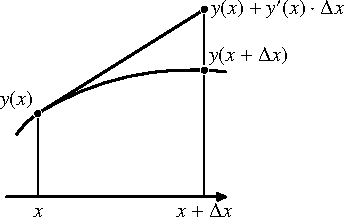
\includegraphics{chapters/images/numerik-2.pdf}
\caption{Lineare Approximation von $y(x+\Delta x)$ durch Information,
die am Punkt $x$ verf"ugbar ist.
\label{numerik:lineareapproximation}}
\end{figure}
Wir versuchen die Differentialgleichung
\begin{equation}
y'=-\alpha y,\qquad y(0)=y_0
\label{numerik:expdgl}
\end{equation}
numerisch zu l"osen. 
Dazu unterteilen wir die $x$-Achse in diskrete Abschnitte der L"ange $h$,
und bezeichnen die Teilpunkte mit $x_k=kh$.
Das Ziel ist jetzt, $y(x_k)$ n"aherungsweise zu berechnen.
Wir schreiben $y_k$ f"ur die N"aherungswerte von $y(x_k)$.
Die Ableitung liefert eine lineare Approximation f"ur $y(x)$,
n"amlich
\[
y(x+\Delta x)\simeq y(x) + y'(x)\cdot\Delta x
\]
(Abbildung~\ref{numerik:lineareapproximation}).
F"ur die Punkte $x_k$ bedeutet das
\[
y(x_{k+1})\simeq y(x_{k})+y'(x_k)\dot h.
\]
Die Differentialgleichung liefert Werte f"ur $y'(x_k)$ aus $x_k$ und $y(x_k)$,
damit k"onnen wir aus dieser Approximation ein allgemeines
N"aherungsverfahren f"ur die L"osung einer Differentialgleichung
konstruieren.

\begin{satz}[Euler-Verfahren]
\index{Euler-Verfahren}
Die Differentialgleichung
\begin{equation}
y'=f(x,y),\qquad y(0)=y_0
\label{numerik:eulerdgl}
\end{equation}
und die Schrittweite $h$ definieren eine Folge 
\[
y_{\mathstrut k}=y_{k-1} + h\cdot f(x_{k-1}, y_{k-1}),\quad k>0,
\]
mit $x_k=kh$,
die eine N"aherung f"ur die Funktionswerte $y(x_k)$ der L"osung $y(x)$
der Differentialgleichung~(\ref{numerik:eulerdgl}) ist.
\end{satz}

Dieses Verfahren ist nicht besonders gut, wie wir im Folgenden zeigen
wollen.
Die Diskussion soll uns aber zeigen, worauf bei der Weiterentwicklung
des Verfahrens geachtet werden muss.

Im vorliegenden Beispiel liefert die
Differentialgleichung~(\ref{numerik:expdgl})
den Wert $y'(x_k)=-\alpha y(x_k)$ f"ur die Ableitung,
woraus wir die Rekursionsformel
\[
y_{k+1}=y_k - \alpha y_k \dot h.
\]
gewinnen.
Die Rekursionsgleichung kann in diesem Fall exakt gel"ost werden,
und wir finden
\begin{equation}
y(x_{k+1}) = y(x_k)-\alpha y(x_k) h=(1-\alpha h) y(x_k)=\dots
=(1-\alpha h)^{k+1}y_0
\label{numerik:rekursion}
\end{equation}
f"ur die N"aherung $y_k$ der Funktionswerte $y(x_k)$.
%Angewendet auf eine beliebige Differentialgleichung, ist dieses
%einfache numerische Verfahren bekannt als das {\em Euler-Verfahren}.
%Es ist nicht besonders genau, aber soll in diesem Abschnitt dazu
%dienen, die Anforderungen an ein gutes numerisches Verfahren
%zu illustrieren.



Wir m"ochten $y(x)$ f"ur einen ganz bestimmten $x$-Wert berechnen.
Dazu unterteilen wir das Interval $[0,x]$ in $n$ Teilschritte der
Breite $x/n$, und wenden die Formel~(\ref{numerik:rekursion}) an:
\[
y(x)=y(x_n)=(1-\alpha h)^n y_0=\biggl(1+\frac{-\alpha x}{n}\biggr)^n y_0.
\]
F"ur eine grosse Zahl von Teilschritten erhalten wir so tats"achlich die
korrekte L"osung:
\[
\lim_{n\to\infty}y_0\biggl(1+\frac{-\alpha x}n\biggr)^n=y_0 e^{-\alpha x}.
\]
\begin{figure}
\centering
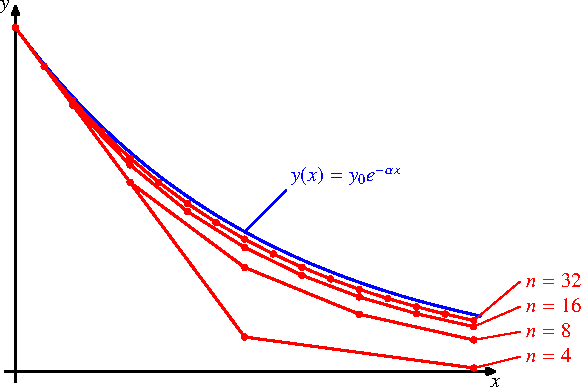
\includegraphics{chapters/images/numerik-1.pdf}
\caption{Approximationen der L"osung der Differentialgleichung $y'=-\alpha y$
mit verschiedener Anzahl Schritte (rot) n"ahern sich f"ur wachsendes
$n$ der exakten L"osung (blau).
\label{numerik:approximation}}
\end{figure}%
Abbildung~\ref{numerik:approximation} zeigt, wie die
durch~(\ref{numerik:rekursion}) gegebenen Approximationen mit zunehmendem
$n$ der exakten L"osung $y(x)=e^{-\alpha x}$ n"aher kommen.

Wir k"onnen auch den Fehler des numerischen Verfahrens berechnen.
Bei der Schrittweite $h$ ist der Fehler von $y_k$ die Differenz
\[
y(x_k)-y_k
=
y_0e^{-\alpha kh}-y_0(1-\alpha h)^k
=
y_0((e^{-\alpha h})^k - (1-\alpha h)^k)
=
y_0e^{-\alpha hk}\biggl(
1-\biggl(\frac{1-\alpha h}{e^{-\alpha h}}\biggr)^k
\biggr).
\]
Man beachte, dass der Z"ahler $1-\alpha h$ die Approximation
$y_1$ ist, als eine Approximation von $e^{-\alpha h}$, dem Nenner.
Schreiben wir
\[
q=\frac{1-\alpha h}{e^{-\alpha h}},
\]
f"ur den Quotienten zwischen der Approximation und dem korrekten Wert,
dann ist sicher immer $q<1$.
Den Fehler k"onnen wir jetzt schreiben
\[
y(x_k)-y_k = y_0e^{-\alpha hk}(1-q^k) = y(x_k)(1-q^k).
\]
Der relative Fehler des Verfahrens ist also
\[
\frac{y(x_k)-y_k}{y(x_k)}=(1-q^k).
\]
\begin{figure}
\centering
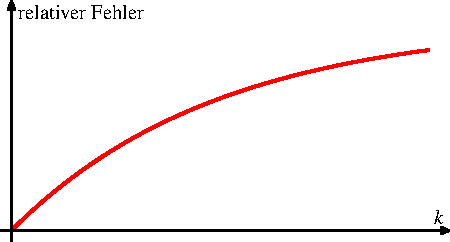
\includegraphics{chapters/images/numerik-3.pdf}
\caption{Relativer Fehler des Eulerverfahrens f"ur die Differentialgleichung
(\ref{numerik:expdgl}) in Abh"angigkeit von der Anzahl $k$ der Schritte.
\label{numerik:relfehler}}
\end{figure}%
Ganz unabh"angig von der Schrittweite $h$ wird der relative Fehler
des Verfahrens immer gegen 1 streben, der Fehler wird also von der
gleichen Gr"ossenordnung wie die berechneten Resultate.

Die Abbildung~\ref{numerik:relfehler} zeigt, dass zu Beginn des Verfahrens
der relative Fehler ungef"ahr linear mit der Anzahl der Schritt zunimmt.
Um eine angemessene Genauigkeit "uber einen gr"osseren Bereich
zu erreichen, muss das Euler-Verfahren also sehr viel kleinere Schritte
und eine entsprechend gr"ossere Anzahl von Schritten ausf"uhren,
die entsprechend viel Rechenzeit ben"otigen.

Ein praktisch n"utzliches Verfahren muss also anstreben, mit einer
sehr viel kleineren Anzahl von Schritten eine viel gr"ossere Genaugikeit
der Approximations zu erreichen.

\section{Fehler-Entwicklung numerischer L"osungen}
\lhead{Fehler-Entwicklung}
Wir betrachten wieder die Differentialgleichung~(\ref{numerik:eulerdgl})
und versuchen, den Fehler eines N"aherungsverfahrens zu bestimmen,
welches Schritte der Gr"osse $h$ durchf"uhrt, um den Wert $y(x)$
zu approximieren.

Das Euler-Verfahren verwendet Schritte der Form
\[
y_{k+1}=y_{k\mathstrut} + hf(x_{k\mathstrut},y_{k\mathstrut}).
\]
In jedem einzelnen Schritt entsteht ein Fehler, dessen Gr"osse wir
aus der Taylor-Entwicklung
\[
y(x+\Delta x)=
y(x) + y'(x)\cdot \Delta x + R(x) \Delta x^2
\]
absch"atzen k"onnen.
Die Funktion $R(x)$ ist beschr"ankt und beschreibt den verbleibenden
Fehler.
Um $y(x)$ zu approximieren, m"ussen $n=x/h$ Schritte der Schrittweite
$h$ durchgef"uhrt werden, von denen jeder einen Fehler
von der Gr"ossenordnung $R(x)h^2$ hat.
Der Gesamtfehler ist daher von der Gr"ossenordnung
\[
y(x)-y_n=O\biggl(R(x)h^2\frac{x}h\biggr)=O(h),
\]
er ist also von erster Ordnung in $h$.
Um eine zus"atzliche Stelle Genauigkeit zu erhalten, muss man also zehnmal
so viele Schritte von zehnmal kleinerer Gr"osse durchf"uhren,
wodurch auch wieder Rundungsfehler eingef"uhrt werden.

K"onnte man den Fehler des Einzelschrittes wesentlich verkleinern, w"urde
auch die Abh"angigkeit des Fehlers des Verfahrens vorteilhafter.
W"are der Fehler des Einzelschrittes $O(h^k)$ statt $O(h^2)$, dann
w"are der Gesamtfehler des Verfahrens nur noch $O(h^{k-1})$.
F"ur $k=3$ bedeutet dies, dass eine Halbierung der Schrittweite
zwar doppelt so viele Schritte braucht, aber auch, dass in jedem
Schritt nur ein Achtel des Fehlers auftritt.
Der Gesamtfehler ist also nur ein Viertel.
Mit zehnmal mehr Arbeit kann man also nicht nur eine Stelle an
Genauigkeit gewinnen, sondern gleich deren zwei.

Man nennt ein Verfahren, bei dem der Gesamt-Fehler von der Gr"ossenordnung
$O(h^k)$ ist, von einem Verfahren $k$-ter Ordnung.
Das Euler-Verfahren ist also ein Verfahren erster Ordnung oder ein
lineares Verfahren.
In der Praxis werden Verfahren bis zu vierter und f"unfter Ordnung
verwendet, so dass eine zehnmal kleinere Schrittweite zu gleich
vier Stellen Genauigkeitsgewinn f"uhren.
Das Ziel der kommenden Abschnitte muss daher sein, einfach
berechnebare Approximationen der Funktion mit m"oglichst geringen
Einzelschrittfehlern zu finden.

\section{Einschritt-Verfahren\label{section:numerik:einschritt}}
\lhead{Einschritt-Verfahren}
Die relativ geringe Genauigkeit des Eulerschrittes beruht darauf,
dass die zu Beginn des Schrittes berechnete Ableitung $f(x_k,y_k)$
nur f"ur das linke Ende des Intervals $[x_k, x_k+h]$ zutrifft,
weiter rechts im Interval wird die Abweichung immer gr"osser.
Eine m"ogliche L"osung des Problems k"onnte darin bestehen, statt
nur einer linearen N"aherung zus"atzliche Glieder der Taylorreihe
\begin{equation}
y(x+\Delta x)
=
y(x)
+
y'(x)\cdot \Delta x
+
\frac12 y''(x)\cdot \Delta x^2
+
\frac16 y'''(x)\cdot \Delta x^3
+
o(\Delta x^3)
\label{numerik:taylor}
\end{equation}
zu verwenden.
In (\ref{numerik:taylor}) werden h"ohere Ableitungen von $y(x)$ ben"otigt,
w"ahrend die Differentialgleichung nur die erste Ableitung liefert.
Die h"oheren Ableitungen wurden aber bereits im
Abschnitt~\ref{grundlagen:hoehere-ableitungen} berechnet.

Wir untersuchen, wie sich das Verfahren f"ur die Beispiel-Gleichung
(\ref{numerik:expdgl}) anwenden l"asst.
Dort gilt
\begin{equation*}
\begin{aligned}
y'(x)&=f(x,y)=-\alpha y
\\
\Rightarrow\qquad
\frac{\partial f}{\partial x}&=0&\frac{\partial f}{\partial y}&=-\alpha
\end{aligned}
\end{equation*}
Alle zweiten Ableitungen verschwinden.
Die Gleichungen werden damit einfach:
\begin{align*}
y''(x)&=-\alpha f(x,y)=\alpha^2 y
\\
y'''(x)&=\alpha^2f(x,y)=-\alpha^3 y.
\end{align*}
Statt der linearen Approximation sollte daher die kubische Approximation
\begin{equation}
y_{k+1}
=
y_{k}-\alpha h y_k +\frac12\alpha^2 h^2 y_k -\frac16 \alpha^3h^3 y_k
=
y_{k}\underbrace{\biggl(1-\alpha h +\frac12\alpha^2h^2 -\frac16 \alpha^3h^3\biggr)}_{\simeq e^{-\alpha h}}
\label{numerik:kubisch}
\end{equation}
verwendet werden.
Dass man hier mit einer gr"osseren Genauigkeit rechnen darf ist schon daran
erkennbar, dass der Klammerausdruck auf der rechten Seite eine viel
bessere Approximation von $e^{-\alpha x}$ ist also der Faktor
$(1-\alpha h)$ im Euler-Verfahren.
Genauer erwarten wir, dass wir hier ein kubsisches Verfahren konstruiert haben.

\begin{table}
\centering
\begin{tabular}{|r|c|r|r|r|}
\hline
$i$&$x$&$e^{-\alpha x}$&Euler&kubisch\\
\hline
 1 & 0.1 & 0.95122942 & 0.\underline{95}000000 & 0.\underline{951229}17 \\
 2 & 0.2 & 0.90483742 & 0.\underline{90}250000 & 0.\underline{904836}93 \\
 3 & 0.3 & 0.86070798 & 0.\underline{85}737500 & 0.\underline{860707}28 \\
 4 & 0.4 & 0.81873075 & 0.\underline{81}450625 & 0.\underline{818729}87 \\
 5 & 0.5 & 0.77880078 & 0.\underline{77}378094 & 0.\underline{778799}73 \\
 6 & 0.6 & 0.74081822 & 0.\underline{73}509189 & 0.\underline{74081}702 \\
 7 & 0.7 & 0.70468809 & 0.\underline{6}9833730 & 0.\underline{70468}675 \\
 8 & 0.8 & 0.67032005 & 0.\underline{6}6342043 & 0.\underline{67031}859 \\
 9 & 0.9 & 0.63762815 & 0.\underline{6}3024941 & 0.\underline{63762}660 \\
10 & 1.0 & 0.60653066 & 0.\underline{5}9873694 & 0.\underline{60652}902 \\
\hline
\end{tabular}
\caption{N"aherungswerte f"ur die L"osung $e^{-\alpha x}$ der
Beispieldifferentialgleichung (\ref{numerik:expdgl}) nach dem Eulerverfahren
und nach dem kubischen Verfahren (\ref{numerik:kubisch}) mit einer
Schrittweite von 0.1. Unterstrichen ist jeweils die Stellen, die nach
Rundung auf die angegebene Anzahl stellen mit dem exakten Wert "ubereinstimmt.
\label{numerik:euler-kubisch}}
\end{table}%
In Tabelle~\ref{numerik:euler-kubisch} werden die Resultate des
kubischen Verfahrens denen des Euler-Verfahrens gegen"ubergestellt.
Im ersten Schritt ist der Fehler des Eulerverfahrens kleiner als $10^{-2}$,
was einer Einheit in der zweiten Nachkommastelle entspricht.
Der Fehler des kubischen Verfahrens ist kleiner als $10^{-6}$, eine
Einheit in der sechsten Nachkommanstelle, ungef"ahr die von einem
kubischen Verfahren zu erwartende Verbesserung.
Nach zehn Rechenschritten liefert das Euler-Verfahren dank Rundung
gerade noch eine korrekte Stelle, w"ahrend das kubische Verfahren immer noch
gerundet f"unf korrekte Stellen gibt.

Es wurde bereits darauf hingewiesen, dass die Terme f"ur die Ableitungen
sehr kompliziert werden.
noch viel gravierender ist allerdings, dass auch die partiellen Ableitungen
von $f$ nach $x$ und $y$ bekannt sein m"ussen.
Es ist zwar im Prinzip m"oglich, diese zu berechnen, der Rechenaufwand 
daf"ur kann aber so erheblich sein, dass er den Genauigkeitsgewinn
leicht wieder zunichte machen kann.
Praktisch n"utzliche Verfahren m"ussen daher danach streben,
die h"oheren Ableitungen von $y(x)$ ausschliesslich aus Funktionswerten
von $f(x,y)$ zu berechnen.

Wir m"ochten aber weiterhin nur $y_{k+1}$ ausschliesslich aus $x_k$ und $y_k$
berechnen, also in einem einzelnen Schritt der Form
\[
y_{k+1}=y_k + h\, F(x_k, y_k, h).
\]
Die Funktion $F(x,y,h)$ heisst die {\em Inkrement-Funktion}
\index{Inkrement-Funktion}
des Verfahrens.
F"ur das Euler-Verfahren ist $F(x,y,h)=f(x,y)$.
Es soll also eine Inkrement-Funktion gefunden werden, bei der $y(x+\Delta x)$
durch $y(x) + \Delta x\cdot F(x,y,\Delta x)$ bis auf Terme h"oherer
Ordnung approxmiert werden kann.

\subsection{Quadratische Verfahren}
Ein quadratisches Verfahren verwendet eine Inkrement-Funktion $F(x,y,h)$,
welche
\[
y(x+h)=y(x)+hF(x,y,h)+O(h^3)
\]
erf"ullt.
Aus den einleitenden Bemerkungen von~\ref{section:numerik:einschritt}
folgt, dass dieses Ziel m"oglicherweise dadurch erreicht werden kann,
dass man Werte von $f$ f"ur verschiedene $x$ geeignet miteinander
kombiniert.
Ein denkbarer Ansatz daf"ur ist
\[
F(x,y,h)=af(x,y) + bf(x+\alpha h, y +\beta hf(x,y)),
\]
oder anders ausgedr"uckt: Man f"uhrt zuerst etwas "ahnliches wie einen
Eulerschritt durch, um zum Punkt $(x+\alpha h,y+\beta hf(x,y))$ zu
gelangen.
Dort berechnet man den Wert von $f$, und bildet dann einen geeigneten
Mittelwert davon  mit $f(x,y)$.
Durch geeignete Wahl von $a$, $b$, $\alpha$ und $\beta$ sollte es m"oglich
sein, dass die Inkrement-Funktion einen Fehler h"ochstens dritter Ordnung
hat, womit wir dann ein Integrationsverfahren zweiter Ordnung gewonnen
h"atten.

Wir m"ussen jetzt die Parameter $a$, $b$, $\alpha$ und $\beta$ bestimmen.
Da wir mit dem "ubereinstimmen der ersten zwei Ableitungen
nur zwei Bedingungen haben, k"onnen wir nicht erwarten, dass wir
eine eindeutige L"osung finden werden.
Vielmehr werden einzelne Parameter frei w"ahlbar sein, es wird eine
ganze Familie von quadratischen L"osungsverfahren entstehen, parametrisiert
durch eine der Variablen $a$, $b$, $\alpha$ und $\beta$.

Wir berechnen nun $F(x,y,h)$ bis zur zweiten Ordnung, damit wird 
$y(x+h)$ bis zur dritten Ordnung ausdr"ucken k"onnen.
\begin{align*}
f(x+\alpha h, y + \beta h f(x,y))
&=
f(x,y)+\alpha h\frac{\partial f(x,y)}{\partial x}
+ \beta h \frac{\partial f(x,y)}{\partial y} + O(h^2)
\end{align*}
\begin{align}
F(x,y,h)
&=
af(x,y) + bf(x+\alpha h, y + \beta h f(x,y))
\notag
\\
&=
(a+b)f(x,y) + \biggl(\alpha b\frac{\partial f(x,y)}{\partial x}
+ \beta b\frac{\partial f(x,y)}{\partial y} f(x,y))\biggr)h+O(h^2)
\label{numerik:inkrementF}
\end{align}
Damit dies bis zur zweiten Ordnung mit dem Inkrement zwischen $x$ und $x+h$
"ubereinstimmt, muss~(\ref{numerik:inkrementF}) mit der Taylorreihe
von $y(x)$ "ubereinstimmen, also mit
\begin{equation}
\frac{y(x+h)-y(x)}{h}=y'(x) + \frac12y''(x)h + O(h^2)
=f(x,y) + \frac12\frac{\partial f(x,y)}{\partial x}
+\frac12\frac{\partial f(x,y)}{\partial y}f(x,y) + O(h^2),
\label{numerik:ytaylor}
\end{equation}
wobei wir f"ur $y''(x)$ die Gleichung (\ref{grundlagen:2abl}) verwendet haben.
Durch Koeffizientenvergleich finden wir die Bedinungen
\[
\begin{aligned}
a+b&=1,&
\alpha b&=\frac12,&
\beta b&=\frac12.
\end{aligned}
\]
Einzig $b$ kommt in allen drei Gleichungen vor, und bestimmt den Wert der
jeweiligen anderen Variablen:
\[
\begin{aligned}
a&=1-b,&\alpha&= \beta=\frac{1}{2b}.
\end{aligned}
\]
Jeder Wert von $b$ zwischen $0$ und $1$ liefert ein Verfahren mit quadratischer
Genauigkeit.

Der Parameterwert $b=1$ f"uhrt auf $\alpha=\beta=1$ und $a=0$, die
Rekursionsformel ist in diesem Falle
\begin{equation}
y_{k+1}=y_{k}+hf\biggl(x_k+\frac{h}2,y_k+\frac{h}2 f(x_k,y_k)\biggr).
\label{numerik:improved-euler}
\end{equation}
Das Verfahren f"uhrt also erst einen halben Eulerschritt zum Punkt
$(x_k+\frac12h,y_k+\frac{h}2f(x_k,y_k))$ durch, berechnet dort mit Hilfe
von $f$ die Steigung, die dann f"ur einen Euler-Schritt der L"ange $h$
verwendet wird.u
Daher heisst dieses Verfahren auch das {\em verbesserte Euler-Verfahren}.
\index{Euler-Verfahren!verbessertes}

Verwendet man $b=\frac12$, folgt zun"achst $a=\frac12$ und $\alpha=\beta=1$.
Daraus erh"alt man die Rekursionsformel
\begin{equation}
y_{k+1}=y_k+\frac{h}2\biggl(
f(x_k,y_k) + f(x_k+h, y_k + hf(x_k,y_k))
\biggr)
\label{numerik:simplified-runge-kutta}
\end{equation}
In diesem Verfahren f"uhrt man also zuerst einen Eulerschritt der L"ange
$h$ durch, mit dem man zum Punkt $(x_k+h, y_k+hf(x_k,y_k))$ gelangt.
Dort berechnet mit mit Hilfe von $f$ die Steigung.
Das arithmetische Mittel dieser Steigung mit der im Euler-Verfahren
verwendeten Steigung $f(x_k,y_k)$ im Punkt $x_k$ wird dann als
Steigung f"ur einen Euler-Schritt verwendet.z
Statt eines einzigen Steigungswertes werden hier also zwei Steigungswerte
von den Enden des Intervals $[x_k,x_k+1]$ gemittelt.
Wegen der "Ahnlichkeit dieses Vorgehens mit dem sp"ater zu besprechenden
Runge-Kutte-Verfahren heisst diese Verfahren auch das {\em
vereinfachte Runge-Kutta-Verfahren}.
\index{Runge-Kutta-Verfahren!vereinfachtes}

\subsection{Runge-Kutta-Verfahren\label{subsection:numerik:runge-kutta}}
\index{Runge-Kutta-Verfahren}
Das {\em Runge-Kutta-Verfahren} erweitert die Inkrement-Funktion derart,
dass der Einzelschritt bis zur f"unften Ordnung mit der Taylorreihe von
$y(x)$ "ubereinstimmt.
So entsteht ein Verfahren vierter Ordnung, es stellt einen guten Kompromiss
zwischen Genauigkeit und Rechenaufwand dar.

Da vier Ableitungen korrekt dargestellt werden m"ussen, ist zu erwarten,
dass vier verschiedene Werte von $f$ an verschiedenen Punkten $(x,y)$
ausgewertet und geeignet miteinander kombiniert werden m"ussen.
Genauer: Man bestimmt zuerst die Werte
\begin{align*}
k_1&=f(x_k,y_k)\\
k_2&=f\biggl(x_k+\frac{h}2,y_k+\frac{h}2k_1\biggr)\\
k_3&=f\biggl(x_k+\frac{h}2,y_k+\frac{h}2k_2\biggr)\\
k_4&=f(x_k+h, y_k+hk_3)
\end{align*}
und setzt diese dann zusammen, um den n"achsten Wert $y_{k+1}$
zu berechnen:
\begin{equation}
y_{k+1} = y_k + h\frac{1}6(k_1 + 2k_2 + 2k_3 + k_4).
\label{numerik:runge-kutta-rekursion}
\end{equation}
Man kann die Formeln wie folgt interpretieren.
Zuerst wird ein halber Eulerschritt mit der Steigung $k_1=f(x_k,y_k)$,
durchgef"uhrt, und und am Zielpunkt die Steigung $k_2$ ermittelt.
Mit dieser Steigung wird dann erneut ein halber Schritt von $(x_k,y_k)$
aus durchgef"uhrt, und am Zielpunkt erneut die Steigung $k_3$ ermittelt.
Damit f"uhrt man einen ganzen Schritt aus, an dessen Zielpunkt man die
Steigung $k_4$ findet.
Diese vier Steigungen werden jetzt gewichtet gemittelt, wobei
$k_2$ und $k_3$ doppeltes Gewicht erhalten, und mit dieser
Steigung wird ein ganzer Schritt vorgenommen.

Die Formeln f"ur die $k_i$ sowie (\ref{numerik:runge-kutta-rekursion})
k"onnen ganz "ahnlich wie das verbesserte Euler-Verfahren bzw.~das
vereinfachte Runge-Kutta-Verfahren begr"undet werden.
Der Aufwand daf"ur ist aber betr"achtlich, so dass wir auf die
detaillierte Darstellung dieser Herleitung verzichten wollen.

\begin{table}
\centering
\begin{tabular}{|r|c|r|r|r|r|r|}
\hline
$i$& $x$ & $y(x)=e^{-\alpha x}$&Euler&verbessert&vereinfacht&Runge-Kutta\\
\hline
 0 & 0.0 & 1.00000000 & 1.000 & 1.00000000 & 1.00000000 & 1.0000000000 \\
 1 & 0.1 & 0.95122942 & 0.\underline{95}0 & 0.\underline{9512}5000 & 0.\underline{9512}5000 & 0.\underline{95122942}71 \\
 2 & 0.2 & 0.90483742 & 0.\underline{90}2 & 0.\underline{9048}7656 & 0.\underline{9048}7656 & 0.\underline{9048374}229 \\
 3 & 0.3 & 0.86070798 & 0.\underline{85}7 & 0.\underline{8607}6383 & 0.\underline{8607}6383 & 0.\underline{8607079}834 \\
 4 & 0.4 & 0.81873075 & 0.\underline{81}4 & 0.\underline{8188}0159 & 0.\underline{8188}0159 & 0.\underline{8187307}620 \\
 5 & 0.5 & 0.77880078 & 0.\underline{77}3 & 0.\underline{7788}8502 & 0.\underline{7788}8502 & 0.\underline{7788007}936 \\
 6 & 0.6 & 0.74081822 & 0.\underline{73}5 & 0.\underline{7409}1437 & 0.\underline{7409}1437 & 0.\underline{7408182}327 \\
 7 & 0.7 & 0.70468809 & 0.\underline{69}8 & 0.\underline{704}79480 & 0.\underline{704}79480 & 0.\underline{7046881}031 \\
 8 & 0.8 & 0.67032005 & 0.\underline{6}63 & 0.\underline{670}43605 & 0.\underline{670}43605 & 0.\underline{6703200}606 \\
 9 & 0.9 & 0.63762815 & 0.\underline{6}30 & 0.\underline{637}75229 & 0.\underline{637}75229 & 0.\underline{6376281}672 \\
10 & 1.0 & 0.60653066 & 0.\underline{5}98 & 0.\underline{606}66187 & 0.\underline{606}66187 & 0.\underline{6065306}762 \\
\hline
\end{tabular}
\caption{Vergleich der Genauigkeit der verbesserten numerischen Verfahren.
Unterstrichen jeweils die nach Rundung korrekten Stellen der L"osung.
\label{numerik:genauigkeit}}
\end{table}


\begin{table}
\centering
\begin{tabular}{|l|l|c|r|>{$}r<{$}|}
\hline
Verfahren                           &$h$  &Schritte&$y_n$&\text{Fehler}\\
\hline
Euler-Verfahren                     &0.025&  40    & 0.\underline{60}462232 &  0.00190834 \\
verbessertes Euler-Verfahren        &0.05 &  20    & 0.\underline{6065}6285 & -0.00003219 \\
vereinfachtes Runge-Kutta-Verfahren &0.05 &  20    & 0.\underline{6065}6285 & -0.00003219 \\
Runge-Kutta-Verfahren               &0.1  &  10    & 0.\underline{6065306}7 & -0.00000001 \\
\hline
\end{tabular}
\caption{Vergleich der verschiedenen Verfahren bei gleichbleibendem 
Rechenaufwand.
Die Schrittweite wurde jeweils so angepasst, dass in allen Verfahren bis
zum Wert $x=1$ die gleiche Anzahl von Auswertungen der Funktion $f$
notwendig wurde.
\label{numerik:vergleich-aufwand}}
\end{table}

Die Tabelle~\ref{numerik:genauigkeit} demonstriert die "uberragende
Genauigkeit des Runge-Kutta-Verfahrens.
Trotz der relativ grossen Schritteweite von $h=0.1$ erreicht das
Verfahren nach zehn Schritten eine Genauigkeit von sieben signifikanten
Stellen.
Da in jedem Schritt die Funktion $f$ viermal ausgewertet werden muss,
ist der Rechenaufwand mit dem Runge-Kutta-Verfahren viermal gr"osser
als im Euler-Verfahren, letzteres kann aber mit nur einer signifikanten
Stelle kaum als brauchbar bezeichnet werden.
Passt man in jedem Verfahren die Schrittweite so an, dass f"ur die
Berechnung der N"aherung f"ur $y(1)$ immer gleich viele Auswertungen
der Funktion $f(x,y)$ n"otig sind, ergeben sich die Resultate in
Tabelle~\ref{numerik:vergleich-aufwand}.
Bei gleichem Rechenaufwand ist das Runge-Kutta-Verfahren um viele
Gr"ossenordungen pr"aziser.
Es gibt daher eigentlich keinen praktischen Grund, "uberhaupt je etwas
anderes als das Runge-Kutta-Verfahren zu verwenden.


\section{Mehrschritt-Verfahren}
\lhead{Mehrschritt-Verfahren}
In den Einschritt-Verfahren wurde wiederholt die Funktion $f$ ausgewertet,
um die Inkrement-Funktion f"ur einen einzigen Schritt zu bestimmen.
Das Ziel dabei war, $y(x+h)$ in "Ubereinstimmung mit der Taylorreihe
bis zu m"oglichst hoher Ordnung zu bestimmen.
Im Runge-Kutta-Verfahren wurden dabei halbe Eulerschritte durchgef"uhrt,
man hat also eigentlich die Aufl"osung nochmals halbiert, um die
Inkrement-Funktion zu ermitteln.
Diese Zwischenwerte geben dem Verfahren die Information "uber die
h"oheren Ableitungen der Funktionen.

Sobald einige Werte der L"osung berechnet sind, l"asst sich die Kr"ummung
der L"osungskurve auch aus diesen Werten ablesen.
Es sollte daher auch m"oglich sein, aus mehreren bereits
ermittelten Werten $y_{n\mathstrut},y_{n+1},\dots,y_{n+s-1}$
den n"achsten Wert $y_{n+s\mathstrut}$ mit der verlangten Genauigkeit
zu berechnen.
Der Vorteil eines solchen Vorgehens ist, dass f"ur jeden Schritt nur 
eine einzige Auswertung der Funktion $f$ n"otig ist,
nicht mehrere wie bei den besprochenen Einschritt-Verfahren.

Als Beispiel versuchen wir daher ein Verfahren aufzubauen, welches
$y_{n+2}$ aus den bereits berechneten Werten $y_{n\mathstrut}$ und
$y_{n+1}$ berechnet.
Wir nehmben dabei an, dass $y_{n\mathstrut}$ und $y_{n+1}$ exakt
sind.
Der neue Datenpunkt soll mit Hilfe eines Ausdrucks der Form
\begin{equation}
y_{n+2}=y_{n+1} + h(af(x_{n+1},y_{n+1}) + b f(x_{n\mathstrut},y_{n\mathstrut}))
\label{numerik:zweischrittansatz}
\end{equation}
gefunden werden.
Die N"aherung kann wieder mit Hilfe der Ableitungen alleine
durch Werte bei $x_{n+1}$ ausgedr"uckt werden:
\begin{align*}
y_{n+2}
&=
y_{n+1}+h(af(x_{n+1}, y_{n+1}) + bf(x_{n+1}-h, y_{n\mathstrut}))
\\
&=
y_{n+1}+haf(x_{n+1}, y_{n+1}) + hbf(x_{n+1}-h, y_{n+1} - h f(x_{n+1},y_{n+1}) + O(h^2))
\\
&=
y_{n+1}+haf(x_{n+1}, y_{n+1}) + hb
\biggl(
f(x_{n+1},y_{n+1})
-h \frac{\partial f(x_{n+1},y_{n+1})}{\partial x}
\\
&\qquad
-h
\frac{\partial f(x_{n+1},y_{n+1})}{\partial y}
f(x_{n+1},y_{n+1})
+ 
\frac{\partial f(x_{n+1},y_{n+1})}{\partial y}
O(h^2)
\biggr)
\\
&=
y_{n+1}
+ (a+b)hf(x_{n+1},y_{n+1})
- bh^2\biggl(
\frac{\partial f(x_{n+1},y_{n+1})}{\partial x}
+
\frac{\partial f(x_{n+1},y_{n+1})}{\partial y}
f(x_{n+1},y_{n+1})
+O(h^3)
\biggr)
\end{align*}
Sie muss bis zur zweiten Ordnung mit der Taylorreihe "ubereinstimmen:
\begin{align*}
y(x_{n+2})
&=
y_{n+1} + hy'(x_{n+1}) + \frac12h^2 y''(x_{n+1})+O(h^3)
\\
&=
y_{n+1}+hf(x_{n+1},y_{n+1})+\frac12h^2\biggl(
\frac{\partial f(x_{n+1},y_{n+1})}{\partial x}
+
\frac{\partial f(x_{n+1},y_{n+1})}{\partial y}
f(x_{n+1},y_{n+1})
\biggr)
\end{align*}
Vergleicht man Koeffizienten, findet man
\[
\begin{aligned}
a+b&=1&-b&=\frac12&&\Rightarrow&a=\frac32
\end{aligned}
\]
Aus der Formel (\ref{numerik:zweischrittansatz}) wird somit die
Iterationsformel
\begin{equation}
y_{n+2}=y_{n+1}+h\biggl(\frac32f(x_{n+1},y_{n+1})
- \frac12 f(x_{n\mathstrut},y_{n\mathstrut})\biggr)
\end{equation}
Diese Rekursionsformel definiert ein quadratisches Verfahren, das
{\em Adams-Bashforth-Verfahren} mit $s=2$.
\index{Adams-Bashforth-Verfahren}

Das Verfahren kann "ahnlich wie das Runge-Kutta-Verfahren auf h"ohere
Ordnung erweitert werden.
Man findet nach einiger Rechnung
\begin{align*}
s&=1\colon&
y_{n+1}
&=
y_n+hf(x_n,y_n)
\\
s&=2\colon&
y_{n+2}
&=
y_{n+1}+h\biggl(\frac32f(x_{n+1},y_{n+1})-\frac12f(x_n,y_n)\biggr)
\\
s&=3\colon&
y_{n+3}
&=
y_{n+2}+h\biggl(\frac{23}{12}f(x_{n+2},y_{n+2})-\frac43f(x_{n+1},y_{n+1})+\frac{5}{12}f(x_n,y_n)\biggr)
\\
s&=4\colon&
y_{n+4}
&=
y_{n+3}+h\biggl(\frac{55}{24}f(x_{n+3},y_{n+3})
	-\frac{59}{24}f(x_{n+2},y_{n+2})
	+\frac{37}{24}f(x_{n+1},y_{n+1})
	-\frac{3}{8}f(x_n,y_n)
\biggr)
\end{align*}
Es ist also m"oglich, ausgehend von dieser Idee Verfahren beliebig hoher
Ordnung zu produzieren.

\begin{table}
\centering
\begin{tabular}{|r|c|r|r|r|r|}
\hline
$i$& $x$ & $y(x)=e^{-\alpha x}$&Euler&Adams-Bashforth&Runge-Kutta\\
\hline
 0 & 0.0 & 1.00000000 & 1.00000000 & 1.00000000 & 1.0000000000 \\
 1 & 0.1 & 0.95122942 & 0.\underline{95}000000 & 0.\underline{9512}8178 & 0.\underline{95122942}71 \\
 2 & 0.2 & 0.90483742 & 0.\underline{90}250000 & 0.\underline{904}93564 & 0.\underline{90483742}29 \\
 3 & 0.3 & 0.86070798 & 0.\underline{85}737500 & 0.\underline{860}84752 & 0.\underline{86070798}34 \\
 4 & 0.4 & 0.81873075 & 0.\underline{81}450625 & 0.\underline{818}90734 & 0.\underline{81873076}20 \\
 5 & 0.5 & 0.77880078 & 0.\underline{77}378094 & 0.\underline{779}01048 & 0.\underline{77880079}36 \\
 6 & 0.6 & 0.74081822 & 0.\underline{73}509189 & 0.\underline{741}05738 & 0.\underline{74081823}27 \\
 7 & 0.7 & 0.70468809 & 0.\underline{69}833730 & 0.\underline{704}95334 & 0.\underline{7046881}031 \\
 8 & 0.8 & 0.67032005 & 0.\underline{6}6342043 & 0.\underline{670}60827 & 0.\underline{6703200}606 \\
 9 & 0.9 & 0.63762815 & 0.\underline{63}024941 & 0.\underline{637}93648 & 0.\underline{6376281}672 \\
10 & 1.0 & 0.60653066 & 0.\underline{59}873694 & 0.\underline{606}85645 & 0.\underline{6065306}762 \\
\hline
\end{tabular}
\caption{Vergleich der Genauigkeit der Verfahren von Euler,
Adams-Bashforth und Runge-Kutta.
Als Startwerte f"ur das Adams-Bashforth-Verfahren wurden die
Werte $y(-h)=e^{-\alpha h}$ und $y(0)=1$ verwendet, um keine zus"atzlichen
Fehler aus der Durchf"uhrung des ersten Schrittes hinzuzuf"ugen.
\label{numerik:genauigkeit-adams-bashforth}}
\end{table}

In der Tabelle~\ref{numerik:genauigkeit-adams-bashforth} wird
das Adams-Bashforth-Verfahren verglichen mit dem lineare Euler-Verfahren 
und dem Verfahren vierter Ordnung von Runge-Kutta.
Die Verbesserung der Genauigkeit des Adams-Bashforth-Verfahrens
gegen"uber dem Euler-Ver\-fah\-ren ist konsistent damit, dass
das Adams-Bashforth-Verfahren ein quadratisches Verfahren ist.

Nachteilig an den Mehrschritt-Verfahren ist die Notwendigkeit,
gen"ugend viele Werte $y_{n},\dots,y_{n+s-1}$ mit ausreichend
hoher Genauigkeit zu bestimmen, bevor das Mehrschritt-Verfahren
seine Schritte der Ordnung $s$ beginnen kann.
Solange diese Werte nicht zur Verf"ugung stehen, kann ein Mehrschritt-Verfahren
nur Schritte niedrigerer Ordnung als $s$ durchf"uhren.

Bei einem Einschritt-Verfahren kann in jedem Schritt die Schrittweite $h$
ver"andert werden, zum Beispiel f"ur Bereiche von $x$-Werten, in denen
die Steigung von $y(x)$ sehr rasch "andert.

F"ur die Beispiel-Differentialgleichung (\ref{numerik:expdgl}) k"onnen
wir das Adams-Bashforth-Verfahren zweiter Ordnung ($s=2$) vollst"andig
analysieren.
Die Rekursionsformel wird zu
\[
y_{n+2}=y_{n+1}+h\biggl(\frac32 (-\alpha y_{n+1})-\frac12(-\alpha y_n)\biggr)
=
\biggl(1-\frac32\alpha h\biggr)
y_{n+1}
+\frac{\alpha h}{2}
y_{n\mathstrut}
\]
Dies ist eine Differenzengleichung mit konstanten Koeffizienten, man kann
sie mit Hilfe eines Potenzansatzes l"osen. 
Wir nehmen also an, dass $y_n=\lambda^n$, und setzen dies in die
Rekursionsformel ein.
Ausserdem k"urzen wir $\alpha h/2=\delta$  ab.
Wir erhalten
\[
\lambda^{n+2}-(1-3\delta)\lambda^{n+1}-\delta\lambda^n=0.
\]
Nach Division durch $\lambda^n$ erhalten wir die quadratische Gleichung
\[
\lambda^2-(1-3\delta )\lambda-\delta=0
\]
f"ur $\lambda$ mit den L"osungen
\[
\lambda_\pm
=
\frac12(1-3\delta) \pm \frac12\sqrt{(1-3\delta)^2+4\delta}.
\]
Da $\delta$ klein ist, wird $\lambda_-$ ebenfalls klein sein,
w"ahrend $\lambda_+$ n"aher bei $1$ sein wird.
Der dominante Einfluss auf die L"osung r"uhrt also von $\lambda_+$ her.
Um diesen Unterschied genauer zu verstehen, verwenden wir eine
lineare Approximation der Wurzel auf der rechten Seite von $\lambda_\pm$:
\begin{align*}
\sqrt{1+x}
&=
1+\frac{x}{2}-\frac{x^2}{4}+\frac{3x^3}{8}-\dots
\\
\sqrt{x}
&=
\sqrt{x_0+x-x_0}
=
\sqrt{x_0}\sqrt{1+\frac{x-x_0}{x_0}}
=
\sqrt{x_0}\biggl(1+\frac12\frac{x-x_0}{x_0}-\frac14\frac{(x-x_0)^2}{x_0^2}+\dots\biggr)
\\
&=
\sqrt{x_0}+\frac12\frac{x-x_0}{\sqrt{x_0}}-\frac14\frac{(x-x_0)^2}{\sqrt{x_0}^3}+\dots
\end{align*}
Wir verwenden diese Approximation mit $x_0=(1-3\delta)^2$ und $x-x_0=-4\delta$
\begin{align*}
\sqrt{(1-3\delta)^2+4\delta}
&=
(1-3\delta)\biggl(1+\frac12\frac{4\delta}{(1-3\delta)^2}
-\frac14\frac{16\delta^2}{(1-3\delta)^4}+\dots\biggr)
\\
&=(1-3\delta)+\frac12\frac{4\delta}{1-3\delta}
-\frac14\frac{16\delta^2}{(1-3\delta)^3}+\dots
\\
&=1-3\delta+2\delta(1+3\delta)-4\delta^2+O(\delta^3)
\\
&=1-3\delta+2\delta + 2\delta^2+O(\delta^3)
\\
&=1-3\delta+2\delta + \frac12(2\delta)^2+O(\delta^3)
\end{align*}
Damit k"onnen wir jetzt $\lambda_+$ bis zur zweiten Ordnung berechnen:
\begin{align*}
\lambda_+
&=
\frac12\biggl((1-3\delta)+ (1-3\delta)+2\delta+\frac12(2\delta)^2\biggr)
+O(\delta^3)
\\
&=
1-2\delta+\frac12(2\delta)^2+O(\delta^3)
\\
&=e^{-2\delta}+O(\delta^3).
\end{align*}
Die exakte L"osung erf"ullt $y_{n+1}=e^{-2\delta}y_n$, der Faktor
$\lambda_+$ stimmt bis auf Terme mindestens dritter Ordnung mit 
$e^{-2\delta}$ "uberein.
Damit ist erneut best"atigt, dass wir es mit einem quadratischen Verfahren zu
tun haben.

Wir k"onnen auch $\lambda_-$ berechnen, und erhalten
\[
\lambda_-=-\delta-2\delta^2+O(\delta^3).
\]
Da $\delta$ klein ist, ist eine Komponente der L"osung bereits nach
drei Schritten kleiner als $O(\delta^3)$, und spielt daher im Vergleich
zu den von $\lambda_+$ herr"uhrenden L"osungen in dritter Ordnung keine
Rolle.

\section{Software}
Die im letzten Abschnitt entwickelten numerischen Verfahren zur L"osung
einer Differentialgleichung kommen ausschliesslich mit Auswertungen der
Funktion $f$ aus, die Ableitungen der Funktion $f$ m"ussen nicht bekannt
sein.
Es sollte also ein Leichtes sein, eine Softwarebibliothek zur
Verf"ugung zu stellen, mit der eine beliebige gew"ohnliche
Differentialgleichung gel"ost werden kann.
Als Input braucht es nur die Funktion $f$ und die Anfangsbedingungen.

Als Beispiel wollen wir in diesem Abschnitt die Differentialgleichung
\[
y''+y=\sin \frac{x}{10},\qquad y(0)=y'(0)=0
\]
in verschiedenen Programmierumgebungen l"osen.
Als erstes bringen wir die Differentialgleichung wieder in die Standardform
einer Vektordifferentialgleichung erste Ordnung:
\begin{equation}
\frac{d}{dt}Y
=
\frac{d}{dx}\begin{pmatrix}y_1\\y_2\end{pmatrix}
=
\begin{pmatrix}
y_2\\
-y_1+\sin\frac{x}{10}
\end{pmatrix}
=
f(x,Y)
\label{numerik:beispieldgl}
\end{equation}
Ein numerisches Verfahren braucht also als Input eine Anfangsbedingung
sowie die Funktion $f$.
Ausserdem muss es M"oglichkeiten bereitstellen, wie man den Gang der
Rechnung beeinflussen kann, z.~B.~um die $x$-Werte anzugeben, f"ur die
die $Y(x)$ bestimmt werden sollen, oder um Genauigkeitsziele zu erreichen.

\subsection{Octave}
In Octave steht eine einzige Funktion \texttt{lsode} zur Verf"ugung, welche
auf zuverl"assige Art Differentialgleichungen l"ost.
Der Anwender muss eine Implementation der Funktion $f$ zur Verf"ugung
stellen, allerdings werden die Argument in der umgekehrten Reihenfolge
zu der erwarte, die wir in diesem Skript bisher verwendet haben.
F"ur die Beispieldifferentialgleichung (\ref{numerik:beispieldgl})
kann man sie zum Beispiel so defniieren:
\verbatiminput{chapters/examples/octave-dgl-f.m}

Beim Aufruf der Funktion \texttt{lsode} muss man den {\em Namen}
der Funktion, die Anfangsbedingung, sowie einen Vektoren mit $x$-Werten,
f"ur die man die L"osung ausgegeben haben m"ochte, als Argumente
"ubergeben.
Der erste Wert im $x$-Vektor muss der $x$-Wert f"ur die Anfangsbedingung
sein, in unserem Fall also $0$.
Um die Werte von $y(x)$ f"ur ganzzahlige Werte von $x$ zu erhalten,
muss man also die Befehle
\verbatiminput{chapters/examples/octave-dgl-sol.m}
ausf"uhren.
Als R"uckgabewert erh"alt man eine Matrix, die in jeder Zeile die
Werte von $y(x)$ und $y'(x)$ zum entsprechenden Wert von $x$
aus dem \texttt{x}-Argument enth"alt.
Die Resultate sind zusammen mit den Werten der exakten
L"osung~(\ref{grundlagen:numerik-beispiel-loesung}) in der dritten Spalte 
in der Tabelle~\ref{numerik:octave-resultate} zusammengestellt.
Es ist gut erkennbar, wie der Fehler anf"anglich langsam ansteigt,
dann aber unter Kontrolle bleibt.
Die Dokumentation der Funktion \texttt{lsode} beschreibt, wie man mit
Hilfe von Optionen ihr Verhalten und insbesondere die Gr"osse der
Fehler weiter beeinflussen kann.
\begin{table}
\centering
\begin{tabular}{|>{$}r<{$}|>{$}r<{$}|>{$}r<{$}|>{$}r<{$}|}
\hline
    x&  y_{\text{numerisch}}(x)&y_{\text{exakt}}(x) & \text{Fehler}\\
\hline
    0&  0.00000000&  0.00000000&  0.00000000\\
    1&  0.00158525&  0.00158528&  0.00000003\\
    2&  0.01090682&  0.01090678&  0.00000003\\
    3&  0.02858723&  0.02858716&  0.00000007\\
    4&  0.04756207&  0.04756212&  0.00000004\\
    5&  0.05957416&  0.05957437&  0.00000020\\
    6&  0.06276426&  0.06276444&  0.00000018\\
    7&  0.06337942&  0.06337932&  0.00000010\\
    8&  0.07002849&  0.07002811&  0.00000037\\
    9&  0.08576626&  0.08576594&  0.00000032\\
   10&  0.10528405&  0.10528416&  0.00000010\\
  100&  0.84661503&  0.84661930&  0.00000427\\
 1000& -0.55228836& -0.55234514&  0.00005678\\
 2000&  0.90392063&  0.90373523&  0.00018540\\
 3000& -0.99018339& -0.99032256&  0.00013917\\
 4000&  0.75185982&  0.75202340&  0.00016358\\
 5000& -0.25298074& -0.25252044&  0.00046030\\
 6000& -0.30093757& -0.30056348&  0.00037408\\
 7000&  0.76905079&  0.76889872&  0.00015207\\
 8000& -1.00327790& -1.00396748&  0.00068958\\
 9000&  0.88860437&  0.88793099&  0.00067338\\
10000& -0.50337856& -0.50335983&  0.00001873\\
\hline
\end{tabular}
\caption{Exakte und numerische L"osung der Beispieldifferentialgleichung
berechnet mit der Funktion \texttt{lsode} von Octave.
\label{numerik:octave-resultate}}
\end{table}

\subsection{GNU Scientific Library}
W"ahrend Octave dem Benutzer die Wahl eines geeigneten Verfahrens abnimmt
und ihm "uberhaupt wenig Kontrolle "uber den Gang der Rechnung gibt,
kann ein Programmier durch den Einsatz der GNU Scientific Library (GSL) die
volle Kontrolle "uber alle Aspekte der Iteration erhalten.
Der Preis ist eine wesentlich h"ohere Komplexit"at.
Ziel dieses Abschnitts ist, ein einfaches Beispielprogramm zu
zeigen, welches als Basis eigener Programme dienen kann.
Es verwendet eine Runge-Kutta-Verfahren achter Ordnung.

Die Funktionen zum L"osen von gew"ohnlichen Differentialgleichungen
der GSL haben alle das Pr"afix \texttt{gsl\_odeiv2\_}. 
Zun"achst braucht es nat"urlich wieder eine Implementation der
Funktion $f$. 
Die GSL "ubergibt zwei Arrays, im einen findet die Funktion die aktuellen
$Y$-Werte, im anderen soll sie die Werte der Ableitung zur"uckgeben.
F"ur die Beispiel-Differentialgleichung (\ref{numerik:beispieldgl})
sieht der Code wie folgt aus:
\verbatiminput{chapters/examples/dgl-f.c}
Der Parameter \texttt{params} dient dazu, der Funktion zus"atzliche
Parameter zu "ubergeben.
In unserem Fall ist das nur die Zahl $\omega$.
Da \texttt{params} ein \texttt{void}-Pointer ist, kann eine beliebige
Struktur zur Parameter"ubergabe verwendet werden.

Die Differentialgleichung wird beschrieben durch eine Struktur vom Typ
\texttt{gsl\_odeiv2\_system}, welche ausser Zeigern auf die Funktion
und die Parameter-Struktur auch noch die Dimension der Vektoren enth"alt.
Es kann auch noch ein Funktionszeiger f"ur eine eine Funktion "ubergeben
werden, die die Jacobi-Matrix berechnet, in unserem Beispiel wird dies
jedoch nicht ben"otigt.

Die eigentliche wird von einer ``driver''-Funktion durchgef"uhrt.
Diese sorgt im wesentlichen f"ur die Wahl der Schrittweite, verwaltet
Datentrukturen, und ruft die Funktionen auf, die die einzelnen Schritte
durchf"uhren.
Die Treiber-Funktion f"uhrt die einzelnen Schritte (im Sinne der
in Abschnitt~\ref{section:numerik:einschritt} besprochenen
Einschritt-Verfahren) mit
Hilfe der Schritt-Funktionen durch, von denen die Bibliothek eine
ganze Reihe bereitstellt.
Die Funktion \texttt{gsl\_odeiv2\_step\_rk4} ist das klassische
Runge-Kutta-Verfahren vierter Ordnung, welches in
Abschnitt~\ref{subsection:numerik:runge-kutta}
beschrieben wurde.
Im Beispielverfahren verwenden wir \texttt{gsl\_odeiv2\_step\_rk8pd},
das Runge-Kutta Prince-Dormand Verfahren achter Ordnung.
F"ur Aufgaben allgemeiner Art ebenfalls sehr gut geeignet ist das
Runge-Kutta-Fehlberg-Verfahren f"unfter Ordnung mit dem Namen
\texttt{gsl\_odeiv2\_step\_rkf45}.
Diese Datenstrukturen werden mit dem Code
\verbatiminput{chapters/examples/dgl-init.c}
initialisiert.
Durch Austausch des zweiten Arguments der Driver-Allozierungs-Funktion
kann man leicht das Verfahren wechseln und so Zeitaufwand und Genauigkeit
f"ur verschiedene L"osungsverfahren vergleichen.

Um die Rechnung durchzuf"uhren, muss jetzt die Driver-Funktion so oft
angewendet werden, wie man Punkt der L"osungskurve ausgeben will.
Dazu dient die Funktion \texttt{gsl\_odeiv2\_driver\_apply}. 
An Argument braucht sie den eben initialisierten Driver, den aktuellen
$x$-Wert, den $x_{\text{next}}$-Wert, f"ur den der n"achste Punkt
ausgegeben werden soll, sowie einen Vektor, in dem der aktuelle Anfangswert
f"ur $Y(x)$ "ubergeben und $Y(x_{\text{next}})$ zur"uckgegeben wird.
$x$ wird als Referenz "ubergeben, wenn die Funktion zur"uckkehrt,
findet man dort den neuen aktuellen Wert von $x$, also im Erfolgsfall
$x_{\text{next}}$.
In unserem Fall brauchen wir $X(x)$ f"ur ganzzahlige $x$, die folgende
Schleife bewerkstelligt dies:
\verbatiminput{chapters/examples/dgl-loop.c}

\begin{table}
\centering
\begin{tabular}{|>{$}r<{$}|>{$}r<{$}|>{$}r<{$}|>{$}r<{$}|}
\hline
    x&  y_{\text{numerisch}}(x)&y_{\text{exakt}}(x) & \text{Fehler}\\
\hline
    1&   0.01584477&   0.01584477&  -0.00000000\\
    2&   0.10882786&   0.10882787&  -0.00000000\\
    3&   0.28425071&   0.28425071&  -0.00000001\\
    4&   0.46979656&   0.46979656&  -0.00000000\\
    5&   0.58112927&   0.58112926&   0.00000001\\
    6&   0.59856974&   0.59856972&   0.00000002\\
    7&   0.58436266&   0.58436265&   0.00000001\\
    8&   0.62466692&   0.62466694&  -0.00000001\\
    9&   0.74961115&   0.74961117&  -0.00000003\\
   10&   0.90492231&   0.90492232&  -0.00000001\\
   20&   0.82626555&   0.82626556&  -0.00000000\\
   30&   0.24234669&   0.24234664&   0.00000005\\
   40&  -0.83971103&  -0.83971092&  -0.00000011\\
   50&  -0.94210772&  -0.94210787&   0.00000015\\
   60&  -0.25144906&  -0.25144893&  -0.00000013\\
   70&   0.58545210&   0.58545205&   0.00000005\\
   80&   1.09974465&   1.09974456&   0.00000009\\
   90&   0.32597838&   0.32597860&  -0.00000023\\
  100&  -0.49836792&  -0.49836823&   0.00000031\\
  200&   1.01037929&   1.01037877&   0.00000052\\
  300&  -0.89702589&  -0.89702630&   0.00000041\\
  400&   0.83859090&   0.83859101&  -0.00000010\\
  500&  -0.21777633&  -0.21777543&  -0.00000090\\
  600&  -0.31235410&  -0.31235239&  -0.00000171\\
  700&   0.72675906&   0.72676124&  -0.00000219\\
  800&  -1.09422992&  -1.09422790&  -0.00000202\\
  900&   0.80223761&   0.80223872&  -0.00000111\\
 1000&  -0.59500324&  -0.59500363&   0.00000040\\
 2000&  -0.97606658&  -0.97606187&  -0.00000471\\
 3000&  -1.03200392&  -1.03199479&  -0.00000914\\
 4000&  -0.79047800&  -0.79047372&  -0.00000428\\
 5000&  -0.37269297&  -0.37270218&   0.00000921\\
 6000&   0.08785158&   0.08783273&   0.00001886\\
 7000&   0.49827647&   0.49826463&   0.00001184\\
 8000&   0.80219750&   0.80220742&  -0.00000992\\
 9000&   0.94568799&   0.94571577&  -0.00002778\\
10000&   0.86607968&   0.86610200&  -0.00002232\\
\hline
\end{tabular}
\caption{L"osungen der Beispieldifferentialgleichg (\ref{numerik:beispieldgl})
mit Hilfe der GNU Scientific Library (GSL).
\label{numerik:gsl-resultate}}
\end{table}

Man kann die Funktion $f$ im Programm nat"urlich auch mit einem Z"ahler
ausstatten und damit herausfinden, wieviele Aufrufe der Funktion
f"ur die numerische L"osung ben"otigt werden.
Es stellt sich heraus, dass f"ur das erste Interval von $0$ bis $1$
die Funktion $f$ 131 mal aufgerufen wird, hier versucht die Bibliothek
die optimale Schrittweite $h$ zu bestimmen.
In allen folgenden Intervallen der L"ange $1$ von $n$ bis $n+1$ werden nur
noch jeweils 13 Aufrufe der Funktion ben"otigt.
Verwendet man stattdessen das Runge-Kutta-Fehlberg-Verfahren,
werden pro Interval 18 Auswertungen der Funktion $f$ ben"otigt,
und die Genauigkeit sinkt auf zwei Stellen nach dem Komma.

\section{Randwertprobleme\label{section:numerik:randwertprobleme}}
Die bisher beschriebenen Verfahren gehen von einer Anfangsbedingung
aus, und berechnen die dadurch eindeutig festgelegte L"osungskurve.
Randwertproblem, beschrieben in Abschnitt~\ref{section:randwertprobleme},
verkn"pfen dagegen Werte von einzelnen Komonenten von $Y$ an den
R"andern eines Intervals.

Wir betrachten zwei prototypische Randwertprobleme, die auch gleich
zwei v"ollig verschiedene L"osungsverfahren motivieren.

\newtheorem{aufgabe}{Aufgabe}[chapter]
\begin{aufgabe}
\label{numerik:aufgabe-ball}
Mit einem nur der Schwerkraft unterworfenen Ball, der im Ursprung des
Koordinatensystems geworfen wird, soll ein Ziel im Punkt $P$ getroffen
werden.
In welcher Richtung und mit welcher Anfangsgeschwindigkeit muss er geworfen
werden?
\end{aufgabe}

Um das Problem einfach zu halten, modellieren wir diese Aufgabe wie
folgt.
Der Ball der Masse $m$ bewegt sich in der $x$-$y$-Ebene, wobei die
Schwerkraft in negativer $y$-Richtung zeigt.
Das Newtonsche Gesetz liefert die Differentialgleichung zweiter Ordnung
\begin{equation}
m\frac{d^2}{dt^2}\begin{pmatrix}x\\y\end{pmatrix}
=
\begin{pmatrix}
0\\-mg
\end{pmatrix}
\label{numerik:ball-dgl}
\end{equation}
Die Masse $m$ kann herausgek"urzt werden.
Gesucht ist eine L"osung so, dass die Bahn durch die Punkte $(0,0)$
und $P=(p,0)$ geht.

Genau genommen ist dies nicht ein Randwertproblem wie in 
Abschnitt~\ref{section:randwertprobleme}, denn es wird nicht verlangt,
dass der Ball zu einer bestimmten Zeit $t$ beim Punkt $P$ eintrift.
Die Differentialgleichung bedeutet aber, dass die Horizontalgeschwindigkeit
des Balls konstant ist (die horizontale Beschleunigung ist immer $0$).
Ist $v_x$ die Horizontalgeschwindigkeit, dann erreicht der Ball zur
Zeit $t_1=p/v_x$ die $x$-Koordinate des Ziels.
Gesucht ist also die anf"angliche Vertikalgeschwindigkeit, die man
dem Ball geben muss, dass zur Zeit $p/v_x$ die $y$-Komponente
der L"osung den Wert $0$ hat.
In dieser Form liegt ein Randwertproblem wie in
Abschnitt~\ref{section:randwertprobleme} vor.

Die L"osungen der Differentialgleichung~\ref{numerik:ball-dgl} sind aus
dem Physik-Unterricht bekannt:
es gilt
\begin{equation}
\begin{pmatrix}x(t)\\y(t)\end{pmatrix}
=
\begin{pmatrix}v_xt\\ v_yt-\frac12gt^2\end{pmatrix}
\end{equation}
Damit l"asst sich auch das Randwertproblem l"osen.
F"ur $t=v_x/p$ muss $y(t)=0$ sein, also
\begin{align}
y(t)=y\biggl(\frac{p}{v_x}\biggr)
=v_y\frac{p}{v_x}-\frac12g\biggl(\frac{p}{v_x}\biggr)^2&=0
\notag
\\
\Rightarrow\qquad
v_y
&=
\frac{v_x}p\frac12g\frac{p^2}{v_x^2}=\frac{gp}{2v_x}.
\label{numerik:ball-bedingung}
\end{align}
Offenbar gibt es zu jedem $v_x$ einen passenden Wert von $v_y$,
mit dem das Ziel getroffen wird.

Die Differentialgleichung (\ref{numerik:ball-dgl}) ist nicht in einer
Form, die der numerischen L"osung zug"anglich ist.
Wir schreiben Sie daher als Differentialgleichung erster Ordnung 
f"ur vierdimensionale Vektoren:
\begin{align}
\frac{d}{dt}Y
=
\frac{d}{dt}\begin{pmatrix}x\\y\\\dot x\\\dot y\end{pmatrix}
&=
\begin{pmatrix}\dot x\\\dot y\\ 0\\ -g\end{pmatrix}.
\label{numerik:ball-dgl-1}
\end{align}
Gesucht ist eine L"osung, die die Randbedingungen
\begin{equation}
Y(0)
=
\begin{pmatrix}0\\0\\v_x\\\color{red}v_y\end{pmatrix},
\qquad
Y\biggl(\frac{p}{v_x}\biggr)
=
\begin{pmatrix}p\\0\\\color{red}?\\\color{red}?\end{pmatrix}
\label{numerik:ball-dgl-2}
\end{equation}
erf"ullt.
Darin stehen die roten Eintr"age f"ur Werte, die nicht vorgegeben sind.
Aus der Symmetrie des Problems kann man nat"urlich auch die Endgeschwindigkeit
ablesen.
Zu bestimmen ist also $v_y$ so, dass die L"osungskurve durch den Punkt
$(p,0)$ geht.

Wird statt der Horizontakomponenten der Anfangsgeschwindigkeit die
gesamte Anfangsgeschwindigkeit $v_0$ vorgegeben, dann muss der
Winkel gefunden werden, unter dem der Ball geworfen werden muss,
um das Ziel zu trefen.
Bei der Elevation $\alpha$ sind die Komponenten der Anfangsgeschwinigkeit
$v_x=v_0\cos\alpha$ und $v_y=v_0\sin\alpha$. 
Setzt man dies in die Bedingung~(\ref{numerik:ball-bedingung}) ein,
findet man
\begin{align*}
v_0 \sin \alpha &=\frac{gp}{2v_0\cos\alpha}
\\
2\sin\alpha\cos\alpha&=\frac{gp}{v_0^2}
\\
\sin2\alpha&=\frac{gp}{v_0^2}
\\
\alpha&= \frac12 \arcsin\frac{gp}{v_0^2}
\end{align*}
Im Nenner rechts steht im wesentlichen die kinetische Energie,
je mehr kinetische Energie der Ball zu Beginn hat, desto kleiner
ist der Winkel, man trifft das Ziel mit einer sehr flachen Bahn.
Kleine Winkel reichen auch f"ur geringe Schwerkraft ($g$ klein)
und kurze Distanzen ($p$ klein).
Die maximale Distanz wird erreicht, wenn das Argument des Arcussinus
den Wert $1$ erreicht, gr"osser darf $p$ nicht werden, weil es sonst
keine L"osung mehr f"ur $\alpha$ gibt.
Die Maximaldistanz ist daher
\[
p_{\text{max}} = \frac{v_0^2}{g}.
\]

\begin{aufgabe}
\label{numerik:aufgabe-seil}
Ein Seil ist zwischen zwei Punkten aufgeh"angt, welche Form nimmt es
allein unter der Wirkung seines Eigengewichtes an?
\end{aufgabe}

\subsection{Schiess-Verfahren\label{numerik:schiess-verfahren}}
Wenn man experimentell versucht, ein Ziel zu treffen, dann wird man
in wiederholten Versuchen die Richtung anpassen, so dass man dem Ziel
immer n"aher kommt.
Der $y$-Wert zur Zeit $p/v_x$ h"angt von der Vertikalgeschwindigkeit ab,
wir bezeichnen ihn mit $h(v_y)$.
Man ver"andert also $v_y$, bis die Gleichung $h(v_y)=0$ erf"ullt ist.
Um das Randwertproblem zu l"osen, muss man also die Gleichung $h(v_y)=0$
numerisch l"osen.

Man kann dies zum Beispiel dadurch machen, dass man nach zwei Werten von $v_y$
sucht, so dass die zum einen geh"orige Bahn unter dem Punkt $P$ durchgeht,
w"ahrend der Ball im anderen Fall dar"uber hinwegfliegt.
Durch wiederholte Halbierung des Intervalls kann man dann den korrekten
Wert f"ur $v_y$ immer genauer eingrenzen%
\footnote{%
Tats"achlich wird dieses Verfahren in der Artillerie verwendet.
Der Schiesskommandant beobachtet die einschlagenden Granaten und kommandiert
"Anderungen der Anfangs-Elevation an die Gesch"utzbatterien.
Dabei sucht er Einschl"age, die aus seiner Perspektive vor bzw.~hinter
dem Ziel liegen, und halbiert dann das Interval, bis die Einschl"age dem
Ziel gen"ugend nahe kommen.}.
Der Nachteil dieses Verfahrens ist, dass mit jedem Schritt die Genauigkeit
nur um in Bit ansteigt, es sind also sehr viele Iterationen notwendig.

Schnellere Konvergenz kann mit dem Newton-Verfahren erreicht werden,
welches in Anhang~\ref{chapter:newton} beschrieben wird.
F"ur die Anwendung des Newton-Verfahrens auf das Randwert-Problem
ist die Bestimmung der Steigung der Funktion n"otig, die die Abweichung
der Kurve von der Randbedingung am rechten Rand angibt.
Wir m"ussen also berechnen, wie schnell sich $y(p/v_x)$ "andert,
wenn $v_y$ ver"andert wird.
Dies ist die Ableitung
\[
h'(v_y)= \frac{\partial y}{\partial v_y},
\]
ein Eintrag der Jacobi-Matrix.
In Abschnitt~\ref{grundlagen:XXX} wurde gezeigt, wie man auch f"ur
die Jacobi-Matrix eine Differentialgleichung aufstellen kann, die
man nat"urlich ebenfalls mit den fr"uher beschriebenen numerischen
Bibliotheken lo"sen kann.

Das Randwertproblem kann daher mit folgendem Algorithmus numerisch gel"ost
werden.
\begin{enumerate}
\item Beginne mit einer Sch"atzung f"ur $v_y$
\item Finde numerisch die L"osung des Anfangswertproblems mit $v_y$
als anf"angliche Vertikalgeschwindigkeit.
Berechnet dabei auch die Jacobi-Matrix
\item Lese die $h(v_y)$ aus der L"osung zur Zeit $p/v_x$ ab, und $h'(v_y)$
aus der Jacobi-Matrix und verwendet den Newton-Algorithmus
(\ref{numerik:ball-newton}), um eine verbesserte Sch"atzung von $v_y$ 
zu bekommen.
\item Wiederhole Schritte 2 und 3 bis die Randbedingung f"ur $t=p/v_x$
gen"ugend genau erf"ullt ist.
\item Die L"osung des Anfangswertproblems mit diesem $v_y$ ist die
L"osung des gestellten Randwertproblems.
\end{enumerate}

\begin{beispiel}
\begin{figure}
\centering
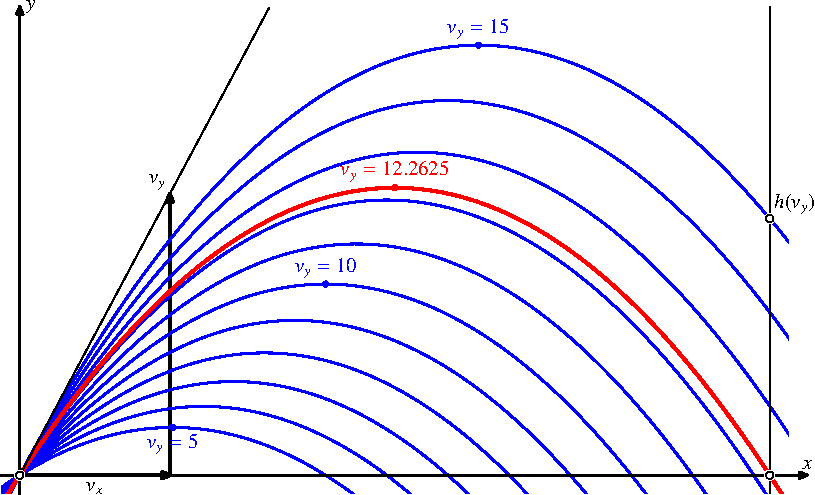
\includegraphics{chapters/images/randwert-1.pdf}
\caption{L"osungen des Anfangswertproblems~(\ref{numerik:ball-dgl-1}) und
(\ref{numerik:ball-dgl-2}).
Das Newton-Verfahren korrigiert $v_y$ derart, dass $h(v_y)=0$ wird.
So wird die L"osung des Randwertproblems (rot) gefunden.
\label{numerik:randwert-bild}}
\end{figure}
Wir f"uhren den eben skizzierten Algorithmus f"ur das Ball-Problem durch.
Um die Jacobi-Matrix zu berechnen, m"ussen wir die Ableitung von $f$ berechnen:
\begin{equation}
\frac{\partial f(x,y)}{\partial y}
=
\begin{pmatrix}
0& 0& 1& 0\\
0& 0& 0& 1\\
0& 0& 0& 0\\
0& 0& 0& 0
\end{pmatrix}.
\end{equation}
Da die rechte Seite nicht von $y$ abh"angt, k"onnen wir die Gleichung f"ur
die Jacobi-Matrix ganz unabh"angig von $y$ l"osen.
Da $F$ so einfach ist, kann man das Matrizenprodukt direkt ausrechnen, 
so wird die Differentialgleichung f"ur $J$
\begin{equation}
\begin{pmatrix}
J'_{11}&J'_{12}&J'_{13}&J'_{14}\\
J'_{21}&J'_{22}&J'_{23}&J'_{24}\\
J'_{31}&J'_{32}&J'_{33}&J'_{34}\\
J'_{41}&J'_{42}&J'_{43}&J'_{44}
\end{pmatrix}
=
\begin{pmatrix}
0& 0& 1& 0\\
0& 0& 0& 1\\
0& 0& 0& 0\\
0& 0& 0& 0
\end{pmatrix}
\begin{pmatrix}
J_{11}&J_{12}&J_{13}&J_{14}\\
J_{21}&J_{22}&J_{23}&J_{24}\\
J_{31}&J_{32}&J_{33}&J_{34}\\
J_{41}&J_{42}&J_{43}&J_{44}
\end{pmatrix}
=
\begin{pmatrix}
J_{31}&J_{32}&J_{33}&J_{34}\\
J_{41}&J_{42}&J_{43}&J_{44}\\
     0&     0&     0&     0\\
     0&     0&     0&     0
\end{pmatrix}
\end{equation}
\begin{table}
\centering
\begin{tabular}{|>{$}r<{$}|>{$}r<{$}|>{$}r<{$}|>{$}r<{$}|>{$}r<{$}|>{$}r<{$}|>{$}r<{$}|>{$}r<{$}|}
\hline
n&    v_y&    t& x(t)&      y(x)&\displaystyle\frac{\partial^{\mathstrut}y}{\partial v_y}&v_{y,\text{new}}&\Delta\\
\hline
0& 7.0000&  2.5& 20.0&-13.156250&  2.5& 12.26250000& -5.2625000000\\
1&12.2625&  2.5& 20.0& -0.000004&  2.5& 12.26250145& -0.0000014458\\
2&12.2625&  2.5& 20.0&  0.000000&  2.5& 12.26250143&  0.0000000204\\
\hline
\end{tabular}
\caption{Newton-Algorithmus f"ur das Ball-Problem, Resultate der numerischen
Rechnung.
$v_y$ wird in drei Schritten mit einer Genauigkeit von mehr als 10 Stellen
gefunden.
\label{numerik:newton-resultate}}
\end{table}%
Daraus kann man ablesen, dass die Elemente $J_{3j}$ und $J_{4j}$ sich
nicht "andern, sie bleiben also konstant.
Aber auch in den ersten zwei Zeilen k"onnen sich nur die Elemente $J_{13}$
und $J_{24}$ "andern, die Differentialgleichungen f"ur diese Elemente
sind
\begin{align*}
J'_{13}&=1\\
J'_{24}&=1
\end{align*}
oder in Matrixform:
\begin{equation}
J(x) = \begin{pmatrix}
1&0&x&0\\
0&1&0&x\\
0&0&1&0\\
0&0&0&1
\end{pmatrix}
\end{equation}
Die L"osung $J_{13}(x)=x$ und $J_{24}=x$.
Damit haben wir die n"otige Information, um den Newton-Algorithmus
durchzuf"uhren.
In Tabelle~\ref{numerik:newton-resultate}
sind die Resultate der numerischen Rechnung zusammengestellt.
Es zeigt sich, dass der korrekte Wert f"ur $v_y$ in drei Iterationen
mit 10 Stellen Genauigkeit gefunden werden kann.
Damit ist das Randwertproblem numerisch gel"ost.
\end{beispiel}





%
% potenzreihen.tex -- Lösung von Differentialgleichungen mit Potenzreihen
%
% (c) 2015 Prof Dr Andreas Mueller, Hochschule Rapperswil
%
\chapter{Potenzreihen-Methode\label{chapter:potenzreihen}}
\rhead{}
\lhead{Potenzreihen-Methode}
Die meisten Differentialgleichungen k"onnen nicht in geschlossener
Form gel"ost werden.
Viele davon sind aber von generischer Bedeutung, sie treten
in verschiedenen Anwendungen immer wieder auf, und verdienen daher
genauer studiert zu werden.
In solchen F"allen kann man die L"osungsfunktionen einfach also
neue interessante Funktionen definieren, ihnen einen Namen geben
und sie verwenden wie zum Beispiel die trigonometrischen Funktionen.
Um sie aber auch berechnen zu k"onnen, braucht man irgend eine 
effiziente Darstellung.
Potenzreihen haben sich daf"ur als besonders geeignet herausgestellt.

In diesem Kapitel wird gezeigt, wie Differentialgleichungen mit Potenzreihen
gel"ost werden k"onnen.
Es zeigt, dass die trigonometrischen Funktionen als Resultat
dieser L"osungsmethode gefunden werden, und es verallgemeinert die
Methode soweit, dass auch kompliziertere Funktionen wie die
Bessel-Funktionen damit verstanden werden k"onnen.

\section{Analytische L"osungen
\label{section:potenzreihen:analytisch}}
\rhead{Analytische L"osungen}
Wir setzen daher die L"osung in Form einer Potenzreihe als
\begin{equation}
y(x)
=
\sum_{k=0}^\infty a_kx^k
\label{potenzreihen:ansatz}
\end{equation}
an, und versuchen die Koeffizienten aus der Differentialgleichung mit
Hilfe eines Koeffizientenvergleichs zu bestimmen.
Die Ableitungen von $y(x)$ sind
\begin{equation}
\begin{aligned}
y'(x)
&=
\sum_{k=1}^\infty a_kkx^{k-1}
=
\sum_{k=0}^\infty a_{k+1}(k+1)x^k
\\
y''(x)
&=
\sum_{k=2}^\infty a_kk(k-1)x^{k-2}
=
\sum_{k=0}^\infty a_{k+2}(k+1)(k+2)x^k 
\\
&\vdots
\end{aligned}
\label{potenzreihen:ableitungen}
\end{equation}

\section{Trigonometrische Funktionen
\label{section:potenzreihen:trigo}}
\rhead{Trigonometrische Funktionen}
Die trigonometrischen Funktionen $\sin x$ und $\cos x$ sind L"osungen
der Schwingungsdifferentialgleichung
\begin{equation}
\begin{aligned}
y''&=-y
&&\text{oder}&
y''+y&=0.
\end{aligned}
\label{potenzreihen:schwingungsdgl}
\end{equation}
Die Potenzreihen-Methode erlaubt uns, direkt Potenzreihen f"ur die
L"osungen von (\ref{potenzreihen:schwingungsdgl}) zu finden.
Wir setzen den Ansatz (\ref{potenzreihen:ansatz}) und die zweite Ableitung
(\ref{potenzreihen:ableitungen}) in die Schwingungsdifferentialgleichung
(\ref{potenzreihen:schwingungsdgl}) ein und erhalten
\begin{equation}
\sum_{k=0}^\infty a_{k+2}(k+1)(k+2)x^k 
+
\sum_{k=0}^\infty a_kx^k
=0.
\end{equation}
Koeffizientenvergleich ergibt die Rekursionsformel
\begin{equation}
\begin{aligned}
\sum_{k=0}^\infty \bigl(a_{k+2}(k+1)(k+2) + a_k\bigr)x^k
&=0
&&\Rightarrow&
a_{k+2}=-a_k\frac1{(k+1)(k+2)}.
\end{aligned}
\end{equation}
Damit die Koeffizienten eindeutig bestimmt sind, m"ussen $a_0$
und $a_1$ festgelegt werden, also der Funktionswert  und die erste
Ableitung bei $x=0$.
Wir finden
\begin{equation*}
\begin{aligned}
a_0&=1,&a_1&=0
&&\Rightarrow&
a_{2k}&=\frac{(-1)^k}{(2k)!},&a_{2k+1}&=0
&&\Rightarrow&
y(x)&=1-\frac{x^2}{2!}+\frac{x^4}{4!}-\dots=\cos x
\\
a_0&=0,&a_1&=1
&&\Rightarrow&
a_{2k}&=0,&a_{2k+1}&=\frac{(-1)^k}{(2k+1)!}
&&\Rightarrow&
y(x)&=x-\frac{x^3}{3!}+\frac{x^5}{5!}-\dots=\sin x,
\end{aligned}
\end{equation*}
die bekannten Taylor-Reihenentwicklungen der trigonometrischen Funktionen.

\section{Verallgemeinerte Potenzreihen
\label{section:potenzreihen:verallgemeinert}}
\rhead{Verallgemeinerte Potenzreihen}
Viele Differentialgleichungen in der Anwendungen sind von der Form
\begin{equation}
x^2y''+p(x)xy'+q(x)y=0,
\label{potenzreihen:verallgemeinert-dgl}
\end{equation}
wobei $p(x)$ und $q(x)$ beliebige Funktionen von $x$ sind.
Das h"aufige Auftreten der Kombinationen $x^2y''$ und $xy'$ in Anwendungen
wird durch ein Dimensionsargument verst"andlich.
Schreiben wir $[u]$ f"ur die Masseinheit einer Gr"osse, dann gilt
\begin{equation*}
\begin{aligned}
\biggl[\frac{dy}{dx}\biggr]
&=
\frac{[y]}{[x]}
&
&\Rightarrow&
[xy']&=[y]\\
\biggl[\frac{d^2y}{dx^2}\biggr]
&=
\frac{[y]}{[x]^2}
&
&\Rightarrow&
[x^2y'']&=[y]
\end{aligned}
\end{equation*}
Wenn zwischen den Termen $x^2y''$, $xy'$ und $y$ irgend ein
gesetzm"assiger Zusammenhang bestehen soll, dann ist die wohl
einfachste Form davon eine lineare Beziehung mit dimensionslosen
Koeffizienten wie in~(\ref{potenzreihen:verallgemeinert-dgl}).

Die Differentialgleichung~(\ref{potenzreihen:verallgemeinert-dgl})
liefert f"ur den Punkt $x=0$ keinen Wert von $y''$.
Eine L"osungsfunktion $y(x)$, die die Differentialgleichung f"ur
$x\ne 0$ erf"ullt, erf"ullt sie f"ur alle $x$, wenn $y(0)=0$ oder
wenn $q(0)=0$ ist. 
Insbesondere haben die Ableitungen an der Stelle $x=0$ keinen
Einfluss darauf, ob die Differentialgleichung erf"ullt ist.
Man spricht auch von einer ausserwesentlichen Singularit"at an
der Stelle $x=0$.
Wir k"onnen allerdings nicht mehr annehmen, dass die L"osung als
Potenzreihe in $x$ geschrieben werden kann, denn eine solche
L"osung w"urde beliebige Ableitungen im Punkt $x=0$ haben, was 
die Differentialgleichung nicht garantieren kann.

\subsection{Verallgemeinerter Ansatz und Indexgleichung}
Setzt man $y(x)$ als Potenzreihe der Form~(\ref{potenzreihen:ansatz}) an,
dann beginnt die Potenzreihe von $x^2y''$ mit dem Term $a_2x^2$,
und $xy'$ beginnt mit $a_1x$.
Daraus folgt, dass nur der Term mit $y$ der
Differentialgleichung~(\ref{potenzreihen:verallgemeinert-dgl})
einen konstanten Term hat, also $a_0=0$.
Teilt man die Differentialgleichung durch $x$ und l"asst $x$ gegen $0$
streben, bekommt man
\begin{align*}
0&=
\lim_{x\to 0}\biggl(
\underbrace{xy''(x)}_{\to 0}+p(x)y'(x)+q(x)\underbrace{\frac{y(x)}{x}}_{\to y'(0)}\biggr)
\\
&=
p(0)y'(0)+q(0)y'(0)
=(p(0)+q(0))a_1
\end{align*}
so dass auch $a_1=0$ sein muss.
Damit kann man auch noch durch $x^2$ teilen und bekommt
\begin{align*}
0&=
\lim_{x\to 0}\biggl(
y''(x)+p(x)\underbrace{\frac{y'(x)}{x}}_{\to y''(0)}+q(x)\frac{y(x)}{x^2}
\biggr)
\\
&=y''(0)+p(0)y''(0)+q(0)a_2
=2a_2+p(0)2a_2+q(0)a_2
=(2+2p(0)+q(0))a_2
\end{align*}
also ist auch $a_2=0$, das Argument l"asst sich offenbar fortsetzen, 
im Allgemeinen wird $a_k=0\;\forall k$ oder $y(x)=0$.
Der einfache Potenzreihenansatz~(\ref{potenzreihen:ansatz}) f"uhrt
daher nicht zum Ziel.

Wir suchen jetzt eine L"osung der
Differentialgleichung~(\ref{potenzreihen:verallgemeinert-dgl})
in Form einer verallgemeinerten Potenzreihe der Form
\begin{equation}
y(x)=x^\varrho\sum_{k=0}^\infty a_kx^k.
\label{potenzreihen:verallgemeinert}
\end{equation}
\index{Potenzreihe!verallgemeinerte}%
Ausser den Koeffizienten $a_k,\;k\ge 0$ ist auch der Exponent
$\varrho$ zu bestimmen.
Das Problem ist so noch nicht eindeutig gestellt, denn es gilt zum Beispiel
\[
x^{-2}\bigl(x^2 + x^3 + x^4 + \dots\bigr)
=
x^{0}\bigl(1+x + x^2 + \dots\bigr),
\]
die gleiche Funktion wurde hier einmal mit $\varrho=-2$ und einmal
mit $\varrho=0$ geschrieben.
Um diese Zweideutigkeit zu vermeiden,
verlangen wir daher zus"atzlich, dass $a_0\ne 0$.

Aus der allgemeinen Theorie der linearen Differentialgleichungen
ist bekannt, dass die Gleichung (\ref{potenzreihen:verallgemeinert-dgl})
zwei linear unabh"angige L"osungsfunktionen haben wird,
welche im Allgemeinen verschiedene $\varrho$ verwenden werden.
Da jede L"osung sich als Linearkombination dieser zwei L"osungen schreiben
l"asst, k"onnen wir f"ur die Basisl"osungen zus"atzlich $a_0=1$ fordern.

Wir k"onnen $y(x)$ und seine Ableitungen auch als
\begin{equation}
\left.
\begin{aligned}
y(x)
&=
\sum_{k=0}^\infty a_kx^{\varrho+k}
\\
y'(x)
&=
\sum_{k=0}^\infty (\varrho+k)a_kx^{\varrho+k-1}
\\
y''(x)
&=
\sum_{k=0}^\infty (\varrho+k)(\varrho+k-1)a_kx^{\varrho+k-2}
\end{aligned}
\right\}
\label{potenzreihen:verallgemeinert-ableitungen}
\end{equation}
schreiben, und vermeiden so eine explodierende Zahl von Termen, die
die Produktregel aus (\ref{potenzreihen:verallgemeinert})
hervorbringen w"urde.
Wir setzen (\ref{potenzreihen:verallgemeinert-ableitungen})
in die Differentialgleichung ein und erhalten
\begin{equation}
\sum_{k=0}^\infty (\varrho+k)(\varrho+k-1)a_kx^{\varrho+k}
+p(x)
\sum_{k=0}^\infty (\varrho+k)a_kx^{\varrho+k}
+q(x)
\sum_{k=0}^\infty a_kx^{\varrho+k}
=0
\label{potenzreihen:verallgemeinert-reihen}
\end{equation}
Die Koeffizienten $a_k$ sollen mit Hilfe eines Koeffizientenvergleichs
bestimmt werden.
Wie in fr"uheren Beispielen kann man nicht erwarten, dass die $a_k$
durch die Differentialgleichung alleine eindeutig bestimmt sind.
Vielmehr ist davon auszugehen, dass die ersten zwei Koeffizienten
als Parameter eingehen, und erst durch die Anfangs- oder Randbedingungen
festgelegt werden k"onnen.

Offenbar m"ussen wir jetzt zus"atzliche Annahmen "uber die
Funktionen $p(x)$ und $q(x)$ machen.
Wir nehmen an, dass sich beide als Potenzreihen schreiben lassen,
wir setzen
\begin{equation*}
\begin{aligned}
p(x)&=\sum_{k=0}^\infty p_kx^k&&\text{und}
&
q(x)&=\sum_{k=0}^\infty q_kx^k.
\end{aligned}
\end{equation*}
Einsetzen in die Gleichungen~(\ref{potenzreihen:verallgemeinert-reihen})
ergibt
\begin{equation*}
\sum_{k=0}^\infty (\varrho+k)(\varrho+k-1)a_kx^{\varrho+k}
+\sum_{s=0}^\infty
\sum_{k=0}^\infty p_s(\varrho+k)a_kx^{\varrho+k+s}
+
\sum_{s=0}^\infty
\sum_{k=0}^\infty q_sa_kx^{\varrho+k+s}
=0.
\end{equation*}
Der kleinste m"ogliche Exponent von $x$ ist $\varrho$, f"ur $k=0$ und $s=0$.
Koeffizientenvergleich in diesem Fall liefert
\begin{equation}
\varrho(\varrho-1)+p_0\varrho +q_0=0,
\label{potenzreihen:indexgleichung}
\end{equation}
wobei wir $a_0=1$ verwendet haben.
Die quadratische Gleichung (\ref{potenzreihen:indexgleichung}) heisst auch die
{\em Indexgleichung}.
\index{Indexgleichung}
Sie hat im allgemeinen zwei verschiedenen L"osungen f"ur die beiden
linear unabh"angigen L"osungen der Differentialgleichungen.

\begin{beispiel}
Als Beispiel nehmen wir an, dass $p(x)=p_0$ und $q(x)=q_0$ konstant sind.
Dann verschwinden die Summen "uber $s$ und die Gleichungen f"ur den
Koeffizientenvergleich besagen nur noch:
\begin{equation}
\begin{aligned}
(\varrho + k)(\varrho+k-1)a_k+p_0(\varrho + k)a_k+q_0a_k&=0
&&\Rightarrow&
((\varrho + k)(\varrho+k-1)+p_0(\varrho + k)+q_0)a_k&=0
\end{aligned}
\end{equation}
auch dies ist eine quadratische Gleichung f"ur $\varrho$, sie wird
aber auch erf"ullt f"ur $a_k=0$ mit $k>0$.
Multiplizieren wir aus, erhalten wir
\[
(\varrho(\varrho - 1) + k\varrho+k(\varrho-1)+k^2+p_0\varrho + p_0k+q_0)a_k=0
\]
Setzen wir die Indexgleichung ein, erhalten wir
\[
(k+(2\varrho-1)+p_0)ka_k=0.
\]
Der Klammerausdruck ist quadratisch in $k$, er verschwindet nur f"ur
die Werte $k=0$ und $k=-p_0-(2\varrho-1)$, es kann also h"ochstens noch
ein weiterer Koeffizient $a_k$ von $0$ verschieden sein, und zwar genau
dann, wenn $-p_0-(2\varrho-1)$ ganzzahlig ist.
\end{beispiel}

\subsection{Doppelte Nullstellen\label{potenzreihen:doppeltens}}
Wenn die Indexgleichung~(\ref{potenzreihen:indexgleichung}) nur eine 
Nullstelle hat, dann kann das eben skizzierte Verfahren auch nur eine
Potenzreihe liefern, obwohl wir bei einer Differentialgleichung
zweiter Ordnung zwei linear unabh"angige L"osungen erwarten.
Es muss daher noch eine weitere L"osung geben, allerdings kann diese
nicht die Form einer verallgemeinerten Potenzreihe haben, sonst h"atte
das Verfahren diese gefunden.

\subsection{Bessel-Gleichung}
Die Besselsche Differentialgleichung
\begin{equation}
x^2y''+xy'+(x^2-n^2)y=0
\label{potenzreihen:verallgemeinert-bessel}
\end{equation}
ist ein Beispiel einer Differentialgleichung der
Form~(\ref{potenzreihen:verallgemeinert-dgl}) mit
$p(x)=1$ und $q(x)=x^2-n^2$.
Die Indexgleichung~(\ref{potenzreihen:indexgleichung}) wird in diesem Fall zu
\begin{equation}
\begin{aligned}
\varrho(\varrho - 1) + \varrho -n^2&=0
&&\Rightarrow&
\varrho^2-n^2&=0
&&\Rightarrow&
\varrho&=\pm n.
\end{aligned}
\label{potenzreihen:bessel-indexgleichung}
\end{equation}
Die Besselsche Differentialgleichung wird also zwei linear
unabh"angige L"osungen
$J_n(x)$ und $J_{-n}(x)$ haben, die in der Form
\[
J_{\pm n}(x)=x^{\pm n}\sum_{k=0}^\infty a_kx^k,\qquad a_0=1
\]
geschrieben werden k"onnen.
Die Funktionen $J_n(x)$ heissen {\em Bessel-Funktionen (erster Art)}.
\index{Bessel-Funktionen erster Art}
\index{Bessel-Funktionen}

Im Fallle $n=0$ hat die
Indexgleichung~(\ref{potenzreihen:bessel-indexgleichung}) eine doppelte
Nullstelle, es gibt dann nur einzige verallgemeinerte Potenzreihe
$J_0(x)$ als L"osung.
Nach der Motivation in Abschnitt~\ref{potenzreihen:doppeltens} erwarten
wir eine weitere L"osung mit einem $\log(x)$-Term.
Wir konstruieren daher den neuen Ansatz
\begin{equation}
y(x)
=
\beta J_0(x)\log(x)+\beta_0+\beta_1x+\beta_2x^2+\beta_3x^3+\dots
\label{potenzreihen:k0ansatz}
\end{equation}
Davon brauchen wir die Ableitungen, 
\begin{align*}
y'(x)
&=
\beta J_0'(x)\log(x) + \beta J_0(x)\frac1x+\beta_1+2\beta_2x+3\beta_3x^2+\dots
\\
y''(x)
&=
\beta J_0''(x)\log(x) + 2\beta J_0'(x)\frac1x-\beta J_0(x)\frac1{x^2} + 2\beta_2 + 3\cdot 2\beta_3 x + 4\cdot 3\beta_4 x^2+\dots
\end{align*}
Die Nenner machen uns keine Sorgen, denn in der Differentialgleichung werden
die Funktionen mit Potenzen von $x$ multipliziert, die die Nenner zum
Verschwinden bringen werden.
Die Schwierigkeit ist eher, den Logarithmus-Term zum Verschwinden zu bringen.
Wir setzen die Funktionen daher in die Differentialgleichung ein:
\begin{align*}
0
&=
x^2y''(x)+xy'(x)+x^2y(x)
\\
&=
\beta x^2J_0''(x)\log(x) + 2x\beta J_0'(x)-\beta J_0(x) + 2\beta_2x^2 + 3\cdot 2\beta_3 x^3 + 4\cdot 3\beta_4 x^4+\dots
\\
&\phantom{=}+
\beta xJ_0'(x)\log(x) + \beta J_0(x)+\beta_1x+2\beta_2x^2+3\beta_3x^4+\dots
\\
&\phantom{=}+
\beta x^2J_0(x)\log(x)+\beta_0x^2+\beta_1x^3 +\beta_2x^4+\beta_3x^5+\dots
\\
&=
\beta(x^2J_0''(x)+xJ_0'(x)+x^2J_0(x))\log(x)
+
\text{Potenzreihe in $x$}
\end{align*}
Der Klammerausdruck in der letzten Zeile ist gerade die Besselsche
Differentialgleichung, und da $J_0(x)$ eine L"osung derselben ist,
verschwindet er.
Damit ist gezeigt, dass die Logarithmus-Terme herausfallen, und mit dem
"ublichen Verfahren des Koeffizientenvergleichs die Koeffizienten
$\beta_k$ einer L"osung bestimmt werden k"onnen.

Setzt man zudem $\beta=1$, kann man die L"osung explizit ermitteln, die
etwas langeweilige Rechnung ergibt
\begin{align*}
K_0(x)
&=
J_0(x)\log(x)
+
\frac{x^2}{2^2}
-
\frac{x^4}{2^2\cdot 4^2}\biggl(1+\frac12\biggr)
+
\frac{x^6}{2^2\cdot 4^2\cdot 6^2}\biggl(1+\frac12+\frac13\biggr)
\\
&\qquad
-
\frac{x^8}{2^2\cdot 4^2\cdot 6^2\cdot 8^2}\biggl(1+\frac12+\frac13+\frac14\biggr)
+
\dots
\label{potenzreihen:k0}
\\
&=
J_0(x)\log(x)
-\sum_{l=1}^\infty (-1)^k\frac{x^{2k}}{(k!\cdot 2^k)^2}\sum_{i=1}^k\frac1s
\end{align*}
Dies ist die Bessel-Funktion 0-ter Ordnung und {\em zweiter Art} (siehe auch
\index{Bessselfunktion zweiter Art}
\cite{skript:smirnow2}).

\section{"Ubungsaufgaben}
\rhead{"Ubungsaufgaben}
\begin{uebungsaufgaben}
\item
\input uebungsaufgaben/401.tex
\item
\input uebungsaufgaben/402.tex
\end{uebungsaufgaben}





%
% linear.tex -- L"osung linearer Differentialgleichungen
%
% (c) 2015 Prof Dr Andreas Mueller, Hochschule Rapperswil
%
\chapter{Differentialgleichungen und lineare Algebra\label{chapter:linear}}
\rhead{}
\lhead{Lineare Differentialgleichungen}
Es lohnt sich, lineare Differentialgleichungen unter Zuhilfenahme
der linearen Algebra etwas genauer zu untersuchen.
Gel"ost werden soll das lineare Differentialgleichungssystem
\begin{equation}
\frac{d}{dt}x = A(t)x + f(t)\qquad x(0)=x_0
\label{linear:gleichung}
\end{equation}
\index{Differentialgleichung!lineare}%
\index{lineare Algebra}%
gel"ost werden.
Darin ist $A(t)$ eine $n\times n$-Matrix.
Wir nehmen der Einfachheit
halber an, dass die Matrixelemente $a_{kl}(t)$ von $A(t)$ differenzierbare
Funktionen von $t$ sind.
Die Funktion $f(t)$ hat $n$-dimensionale Vektoren als Werte.
Falls $f(t)=0$ ist, ist die Gleichung~\eqref{linear:gleichung}
homogen.
\index{Differentialgleichung!homogene}

\section{Konstante Koeffizienten}
\rhead{Konstante Koeffizienten}
In diesem Abschnitt nehmen wir an, dass $A(t)$ konstant ist, wir schreiben
einfach $A$ f"ur den konstanten Wert von $A(t)$.
\subsection{Diagonalisierbare Koeffizientenmatrix}
Besonders einfach w"are \eqref{linear:gleichung} zu l"osen, wenn $A$
Diagonalform h"atte,
\[
A=\begin{pmatrix}
\lambda_1&         &      &         \\
         &\lambda_2&      &         \\
         &         &\ddots&         \\
         &         &      &\lambda_n
\end{pmatrix}.
\]
%Durch Wechsel der Basis kann man diese Situation immer erreichen, wenn
%$A$ diagonalisierbar ist.
%
In diesem Fall zerf"allt das Gleichungssystem in $n$ unabh"angige
lineare Differentialgleichungen erster Ordnung
\begin{align*}
\dot{x}_1&=\lambda_1x_1 + f_1(t)\\
\dot{x}_2&=\lambda_2x_2 + f_2(t)\\
&\;\,\vdots\\
\dot{x}_n&=\lambda_nx_n + f_n(t).
\end{align*}
Die homogenen Gleichungen lassen sich sofort l"osen:
\[
\dot{x}_i=\lambda_ix_i
\qquad
\Rightarrow
\qquad
x_i(t)=x_{0i}e^{\lambda_it}.
\]
Daraus kann man die L"osung des inhomogenen Systems mit Hilfe der
Variation der Konstanten l"osen:
\[
x_i(t)=C_i(t)e^{\lambda_i t}
\qquad
\Rightarrow
\qquad
\dot{x}_i(t)
=
\dot{C}_i(t)e^{\lambda_i t}+C_i(t)\lambda_ie^{\lambda_i t}
=
\lambda_i x_i(t) + \dot{C}_i(t)e^{\lambda_i t}
\]
Die $C_i(t)$ m"ussen also so gew"ahlt werden, dass
$\dot{C}_i(t)=f_i(t)e^{-\lambda_i t}$, es folgt
\[
C_i(t)=x_{0i}+\int_0^t C_i(\tau)e^{-\lambda_i \tau}\,d\tau
\]
und damit die L"osung
\[
x_i(t)
=
\biggl(x_{0i}+\int_0^t C_i(\tau)e^{-\lambda_i \tau}\,d\tau\biggr)
e^{\lambda_i t}.
\]
Diese L"osung hatten wir fr"uher bereits gefunden, doch wollen wir
dies auch noch in Matrixform schreiben.
Dazu setzen wir
\[
e^{At}=\begin{pmatrix}
e^{\lambda_1 t}&               &      &               \\
               &e^{\lambda_1 t}&      &               \\
               &               &\ddots&               \\
               &               &      &e^{\lambda_n t}
\end{pmatrix}.
\]
Mit dieser Schreibweise kann die L"osung geschrieben werden als
\[
x(t)
=
e^{At}
\biggl(x_0 + \int_0^t e^{-A\tau}f(\tau)\,d\tau\biggr)
\]
Wir werden in den n"achsten zwei Abschnitten zeigen, dass diese 
Funktion f"ur beliebige Matrizen $A$ definiert werden kann und
eine L"osung der Differentialgleichung liefert.

\subsection{Matrix-Exponentialfunktion}
\index{Matrix-Exponentialfunktion}%
Die L"osung im vorangegangenen Abschnitt konnte mit Hilfe der
Matrix-Exponentialfunktion besonders kompakt formuliert werden.
Allerdings war diese nur f"ur diagonalisierbare Matrizen definiert.
Wir k"onnten $e^A$ aber auch "uber die Potenzreihe definieren
\[
e^A=E+A+\frac12A+\frac1{3!}A^3+\frac1{4!} A^4+\dots
\]
Die Ableitung von $e^{At}$ nach $t$ ist
\begin{align*}
\frac{d}{dt}e^{At}
&=
\frac{d}{dt}\biggl(E+At+\frac1{2!}t^2A^2+\frac1{3!}t^3A^3+\dots\Biggr)
\\
&=
A+tA^2+\frac12t^2A^3+\frac1{3!}t^3A^4+\dots
\\
&=
\biggl(E+tA+\frac12t^2A^2+\frac1{3!}A^3+\dots\biggr)A
=e^{tA}A=Ae^{At}
\end{align*}
\begin{satz}
\label{linear:matrix-exp}
Die Matrix-Funktion $t\mapsto X(t)=e^{At}$ erf"ullt also die
Matrix-Differentialgleichung
\begin{equation}
\frac{d}{dt} X = AX
\qquad\text{mit}\qquad
X(0)=E.
\label{linear:matrix-dgl}
\end{equation}
\end{satz}

\subsection{Beliebige Koeffizientenmatrix}
Mit der Matrix-Exponentialfunktion kann jetzt auch das homogene
Differentialgleichungssystem gel"ost werden.
Dazu multiplizieren wir~\eqref{linear:matrix-dgl} auf der rechten Seite
mit $x_0$ 
\[
\frac{d}{dt}X(t)x_0 = A X(t)x_0.
\]
Die Funktion
\[
x(t)=X(t)x_0 = e^{At}x_0
\]
ist daher eine L"osung der homogenen Gleichung, der konstante Vektor $x_0$ 
entspricht der Anfangsbedingung.

Auch das Verfahren der Variation der Konstanten kann durchgef"uhrt werden.
\index{Variation der Konstanten}%
Dazu ersetzen wir $x_0$ durch einen Vektor $C(t)$, und leiten den Ansatz
\[
x(t)=e^{At}C(t)
\]
nach $t$ ab
\[
\frac{d}{dt}x(t)
=
Ae^{At}C(t) + e^{At}\dot{C}(t)
=
A x(t) + e^{At}\dot{C}(t)
\]
Damit $x(t)$ eine L"osung ist, muss gelten
\[
\begin{aligned}
e^{At}\dot{C}(t)
&=
f(t)
&&\text{und}
&
C(0)&=x_0
\end{aligned}
\]
Diese Differentialgleichung kann durch Integration gel"ost werden,
wir erhalten
\begin{align*}
\dot{C}(t)
&=
e^{-At}f(t)
\\
\Rightarrow\qquad
C(t)
&=
x_0+\int_0^t e^{-A\tau}f(\tau)\,d\tau
\end{align*}
und damit als L"osung der inhomogenen Differentialgleichung
\[
x(t)
=
e^{At}\biggl(
x_0+\int_0^t e^{-A\tau}f(\tau)\,d\tau
\biggr).
\]
Die fr"uher gefundene Formel f"ur die L"osung der Differentialgleichung
\eqref{linear:gleichung} f"ur den Spezialfall diagonalisierbarer 
Matrizen gilt daher f"ur beliebige Matrizen.
Wir fassen die Resultate dieses Abschnittes im folgenden Satz 
zusammen.

\begin{satz}\label{linear:inhomogeneloesung}
Die Differntialgleichung
\[
\frac{d}{dt}x = A(t)x + f(t)\qquad x(0)=x_0
\]
hat die L"osung
\[
x(t)
=
e^{At}\biggl(
x_0+\int_0^t e^{-A\tau}f(\tau)\,d\tau
\biggr).
\]
\end{satz}

\subsection{Ein wichtiger Spezialfall: Jordan-Normalform}
F"ur einige spezielle Matrizen l"asst sich die Matrix-Exponentialfunktion
direkt berechnen.
Wir beginnen mit folgendem rein algebraischen Resultat, welches wir
sp"ater in einigen n"utzlichen F"allen anwenden.

\begin{definition}
Die Matrix $A(p,q)$ hat die Matrixelemente
\begin{equation}
A(p,q)_{ij}
=
\begin{cases}
0&\qquad i < j-1\\
p&\qquad i = j-1\\
q&\qquad i = j\\
0&\qquad i > j
\end{cases}
\label{linear:apqmatrixelement}
\end{equation}
oder
\begin{equation}
A(p,q)=\begin{pmatrix}
p&q& &      & \\
 &p&q&      & \\
 & &p&\ddots& \\
 & & &\ddots&q\\
 & & &      &p
\end{pmatrix},
\label{linear:apqmatrix}
\end{equation}
nicht dargestellte Matrixelemente sind $0$.
\end{definition}

\begin{satz}
\label{linear:apq}
Die Matrix $A(p,q)^k$ hat die Matrixelemente
\begin{equation}
(A(p,q)^k)_{ij}
=\begin{cases}
\displaystyle \binom{k}{j-i}p^{k-(j-i)}q^{j-i} &\qquad i\le j\\[2mm]
0                                              &\qquad i>j.
\end{cases}
\label{linear:apqk}
\end{equation}
\end{satz}

\begin{proof}[Beweis]
Wir stellen zun"achst sicher, dass die Formel~\eqref{linear:apqk} sinnvoll ist.
F"ur $k=0$ verschwinden alle Binomialkoeffizienten ausser $\binom{k}{0}$,
die Formel~\eqref{linear:apqk} beschreibt dann eine Diagonalmatrix, und
die Diagonalelemente sind $\binom{0}{0}p^0q^0=1$, die Formel~\eqref{linear:apqk}
beschreibt in diesem Fall also die Einheitsmatrix.

Auch f"ur $k=1$ l"asst sich gleichermassen verifizieren, dass die
Formel~\eqref{linear:apqk} in diesem Fall die Matrix $A(p,q)$ beschreibt.
Damit haben wir auch bereits die Verankerung f"ur einen induktiven
Beweis der Formel~\eqref{linear:apqk} gelegt.

F"ur den Induktionsschritt nehmen wir jetzt an, dass die
Formel~\eqref{linear:apqk} f"ur $k$ bereits bewiesen ist, und berechnen
f"ur den Fall $k+1$
die Matrixelemente von $A(p,q)^{k+1}$, indem wir das Matrizenprodukt
ausrechnen.
Da $A(p,q)$ eine obere Dreiecksmatrix ist, werden auch alle Potenzen
$A(p,q)^k$ obere Dreiecksmatrizen sein, was die Formel~\eqref{linear:apqk}
auch ausdr"uckt.
Wir brauchen daher nur Elemente oberhalb der Diagonalen, also f"ur $j\ge i$:
\begin{align*}
(A(p,q)^{k+1})_{ij}
&=
(A(p,q)A(p,q)^k)_{ij}
\\
&=
(\text{Zeile $i$ von $A(p,q)$})
\cdot
(\text{Spalte $j$ von $A(p,q)^k$})
\\
&=
\begin{pmatrix}
0&\dots&p&q&0&\dots
\end{pmatrix}
\begin{pmatrix}
\vdots\\
(A(p,q)^k)_{ij}\\
(A(p,q)^k)_{i+1,j}\\
\vdots
\end{pmatrix}
\\
&=
p(A(p,q)^k)_{ij}
+
q(A(p,q)^k)_{i+1,j}
\\
&=
p\binom{k}{j-i}p^{k-(j-i)}q^{j-i}
+
q\binom{k}{j-(i+1)}p^{k-(j-(i+1))}q^{j-(i+1)}
\\
&=
\left(\binom{k}{j-i}+\binom{k}{j-i-1}\right) p^{k+1-(j-i)}q^{j-i}
\\
&=
\binom{k+1}{j-i} p^{k+1-(j-i)}q^{j-i}
\end{align*}
Damit ist der Induktionsschritt vollzogen und damit die
Formel~\eqref{linear:apqk} bewiesen.
\end{proof}

Die Potenzen von $A(p,q)$ k"onnen jetzt mit Hilfe der Exponentialreihe
dazu verwendet werden, $e^{A(p,q)}$ zu berechnen:

\begin{satz}
\label{linear:apqexp}
Die Matrixelemente von $e^{A(p,q)}$ sind 
\[
e^{A(p,q)}
=
\begin{cases}
\frac1{(j-i)!}q^{j-i}e^p,
 &\qquad i\le j\\
0&\qquad i>j
\end{cases}
\]
\end{satz}

\begin{proof}[Beweis]
Auch $e^{A(p,q)}$ ist wieder eine obere Dreiecksmatrix, wir brauchen also
nur die Matrixelemente mit $i\le j$ zu berechnen:
\begin{align*}
(e^{A(p,q)})_{ij}
&=
\sum_{k=0}^\infty \frac1{k!}\binom{k}{j-i}p^{k-(j-i)}q^{j-i}
\end{align*}
Wir k"urzen $j-i=s$ ab, und beachten, dass der Binomialkoeffizient nur
dann von $0$ verschieden ist, wenn $k\ge j-i=s$ ist.
Es reicht also, mit der Summe bei $k=s$ zu beginnen
\begin{align*}
(e^{A(p,q)})_{ij}
&=
\sum_{k=s}^\infty \frac1{k!}\binom{k}{s}p^{k-s}q^s
=
\sum_{k=s}^\infty \frac1{k!}\frac{k!}{(k-s)!s!}p^{k-s}q^s
=
\frac1{s!}q^s \sum_{k=s}^\infty \frac{1}{(k-s)!}p^{k-s}
\end{align*}
In der Summe kommt nur die Differenz $k-s$ vor, wir schreiben
daher $r=k-s$ und beginnen die Summe bei $r=0$.
Damit finden wir
\begin{align*}
(e^{A(p,q)})_{ij}
&=
\frac1{s!}q^s \sum_{r=0}^\infty \frac{1}{r!}p^r
=
\frac1{s!}q^se^p,
\end{align*}
womit der Satz bewiesen ist.
\end{proof}

Die S"atze~\ref{linear:apq} und \ref{linear:apqexp} k"onnen dazu verwendet
werden, die Potenzen anderer Matrizen zu berechnen, die f"ur die L"osung von
Differentialgleichungssystemen wichtig sind.

\begin{satz}
\label{linear:jnfexp}
Die Matrix
\[
A(\lambda)=\begin{pmatrix}
\lambda&      1&       &      &       \\
       &\lambda&      1&      &       \\
       &       &\lambda&\ddots&       \\
       &       &       &\ddots&      1\\
       &       &       &      &\lambda
\end{pmatrix}
\]
hat die Matrix-Elemente
\[
a_{ij}(\lambda)=\begin{cases}
\lambda&\qquad j=i\\
      1&\qquad j=i+1\\
      0&\qquad \text{sonst.}
\end{cases}
\]
Dann hat die Matrix $A(\lambda)^k$ die Matrixelemente
\begin{equation}
(A(\lambda)^k)_{ij}=\begin{cases}
\displaystyle \binom{k}{j-i}\lambda^{k-(j-i)}&\qquad i\le j\\
0&\qquad i > j,
\end{cases}
\label{linear:ahochk}
\end{equation}
und $e^{A(\lambda)}$ hat die Matrixelemente
\[
(e^{A(\lambda)})_{ij}
=
\begin{cases}
\frac{1}{(j-i)!}e^\lambda &\qquad i\le j\\
0                         &\qquad i>j.
\end{cases}
\]
\end{satz}

\begin{proof}[Beweis]
Dies folgt unmittelbar aus Satz~\ref{linear:apqk} und \ref{linear:apqexp},
indem man $p=\lambda$ und $q=1$ setzt.
\end{proof}

Nicht jede Matrix $A$ ist diagonalisierbar, aber man kann zeigen, dass
durch Wahl einer geeigneten Basis jede Matrix in eine Form gebracht
werden kann, die aus Bl"ocken der Form $A(\lambda)$ auf der Diagonalen
besteht,
\[
\begin{pmatrix}
A_1(\lambda_1)&              &      &              \\
              &A_2(\lambda_2)&      &              \\
              &              &\ddots&              \\
              &              &      &A_s(\lambda_s)
\end{pmatrix},
\]
wobei die Werte $\lambda_i$ die Eigenwerte der Matrix sind.
Diese Form der Matrix heisst die Jordan-Normalform.
\index{Jordan-Normalform}%
F"ur eine Matrix in Jordan-Normalform kann die Matrix-Exponentialfunktion
explizit berechnet werden, man kann also die L"osungen der
zugeh"origen Differentialgleichung direkt angeben.
Allerdings brauchen wir daf"ur nicht nur $e^{A(\lambda)}$, sondern
$e^{tA(\lambda)}$, wie im folgenden Satz.

\begin{satz}
\label{linear:alambdaexp}
Sei $A(\lambda)$ die Matrix wie in Satz~\ref{linear:jnfexp}.
Dann hat $e^{tA(\lambda)}$ die Matrix-Elemente
\[
(e^{tA(\lambda)})_{ij}
=
\begin{cases}
\frac1{(j-i)!}t^{j-i}e^{\lambda t}
 &\qquad i\le j\\
0&\qquad i>j
\end{cases}
\]
\end{satz}

\begin{proof}[Beweis]
Dies ergibt sich aus Satz~\ref{linear:apqexp}, indem man $p=\lambda t$ und
$q=t$ setzt.
\end{proof}

Ausgeschrieben ist dies
\[
e^{tA(\lambda)}
=
\begin{pmatrix}
e^{\lambda t}&te^{\lambda t}&\frac12t^2e^{\lambda t}&      & \\
             & e^{\lambda t}&te^{\lambda t}         &\ddots& \\
             &              &e^{\lambda t}          &\ddots&\frac12t^2e^{\lambda t}\\
             &              &                       &\ddots&te^{\lambda t}\\
             &              &                       &      &e^{\lambda t}
\end{pmatrix}.
\]

\begin{beispiel}
Als Beispiel betrachten wir die homogene Differentialgleichung
\[
y''+2\sigma y'+\sigma^2y=0.
\]
Als Erstes bringen wird diese Gleichung in Vektorform 
\[
Y(x)=\begin{pmatrix}
y(x)\\y'(x)
\end{pmatrix}
\qquad\Rightarrow\qquad
\frac{d}{dx}Y(x)
=
\begin{pmatrix}
y'(x)\\
-2\sigma y'(x)-\sigma^2y(x)
\end{pmatrix}
=
\begin{pmatrix}
0&1\\
-\sigma^2& -2\sigma
\end{pmatrix}
Y(x).
\]
Die Matrix auf der rechten Seite hat das charakteristische Polynom
\index{charakteristisches Polynom}%
\begin{align*}
\left|\,\begin{matrix}
—\lambda&1\\
-\sigma^2&-\lambda-2\sigma
\end{matrix}\,\right|
&=
\lambda(\lambda+2\sigma)+\sigma^2
=
\lambda^2+2\sigma\lambda+\sigma^2=(\lambda+\sigma)^2=0
\\
\Rightarrow\qquad
\lambda&=-\sigma
\end{align*}
Das charakteristische Polynom hat also nur eine Nullstelle.
Wir bestimmen die Eigenvektoren:
\index{Eigenvektor}%
\begin{align*}
\begin{tabular}{|>{$}c<{$}>{$}c<{$}|}
\hline
-\lambda & 1\\
-\sigma^2&-\lambda-2\sigma\\
\hline
\end{tabular}
&=
\begin{tabular}{|>{$}c<{$}>{$}c<{$}|}
\hline
\sigma & 1\\
-\sigma^2&\sigma-2\sigma\\
\hline
\end{tabular}
=
\begin{tabular}{|>{$}c<{$}>{$}c<{$}|}
\hline
\sigma & 1\\
-\sigma^2&-\sigma\\
\hline
\end{tabular}
\rightarrow
\begin{tabular}{|>{$}c<{$}>{$}c<{$}|}
\hline
1&\frac1{\sigma}\\
0&0\\
\hline
\end{tabular}
\qquad\Rightarrow\qquad
v=
\begin{pmatrix}
1\\-\sigma
\end{pmatrix}
\end{align*}
Da es nur einen Eigenvektor gibt, kann die Matrix nicht diagonalisierbar
sein.
Um eine Basis zu konstruieren, in welcher die Matrix Jordan-Normalform
bekommt, brauchen wir eine Vektor $w$, der die Gleichung
\[
Aw = \lambda w + v
\qquad\Rightarrow\qquad
(A-\lambda E)w=w
\]
erf"ullt.
Setzen wir die bekannten Werte ein, suchen wir eine L"osung des
Gleichungssystems
\[
\begin{tabular}{|>{$}c<{$}>{$}c<{$}|>{$}c<{$}|}
\hline
 \sigma  &    1    & 1 \\
-\sigma^2& -\sigma & -\sigma\\
\hline
\end{tabular}
\rightarrow
\begin{tabular}{|>{$}c<{$}>{$}c<{$}|>{$}c<{$}|}
\hline
 \sigma  &    1    & 1 \\
     0   &    0    & 0 \\
\hline
\end{tabular}
\qquad
\Rightarrow
\qquad
w=\begin{pmatrix}
0\\1
\end{pmatrix}
\]
wobei wir f"ur die frei w"ahlbare zweite Variable den Wert $1$ gew"ahlt haben.
In der Basis $B'=\{v, w\}$ hat die Matrix des Differentialgleichungssystems
die Form
\[
A'
=
\begin{pmatrix}
-\sigma&      1\\
      0&-\sigma 
\end{pmatrix}
\]
Die Transformationsmatrix, die von der Standardbasis in die Basis $B'$
\index{Transformationsmatrix}%
umrechnet ist
\[
T
=
\begin{pmatrix}
      1&0\\
-\sigma&1
\end{pmatrix}
\qquad\text{und}\qquad
T^{-1}
=
\begin{pmatrix}
     1&0\\
\sigma&1
\end{pmatrix}.
\]
Tats"achlich kann man nachrechnen, dass
\[
T^{-1}AT
=
\begin{pmatrix}
     1&0\\
\sigma&1
\end{pmatrix}
\begin{pmatrix}
0&1\\
-\sigma^2&-2\sigma
\end{pmatrix}
\begin{pmatrix}
      1&0\\
-\sigma&1
\end{pmatrix}
=
\begin{pmatrix}
     1&0\\
\sigma&1
\end{pmatrix}
\begin{pmatrix}
-\sigma  &1\\
 \sigma^2&-2\sigma
\end{pmatrix}
=
\begin{pmatrix}
-\sigma&1\\
      0&-\sigma
\end{pmatrix}.
\]

Um die Differentialgleichung zu l"osen, brauchen wir die Matrix
$e^{A'x}$, die wir aus Satz~\ref{linear:alambdaexp} ablesen k"onnen:
\begin{align*}
e^{A'x}
&=
\begin{pmatrix}
e^{-\sigma x}&xe^{-\sigma x}\\
       0     & e^{-\sigma x}
\end{pmatrix}
=
\begin{pmatrix}
1&x\\
0&1
\end{pmatrix}
e^{-\sigma x}.
\end{align*}
Diese Matrix transformieren wir mit 
\begin{align*}
Te^{A'x}T^{-1}
&=
e^{-\sigma x}
\begin{pmatrix}
      1&0\\
-\sigma&1
\end{pmatrix}
\begin{pmatrix}
1&x\\
0&1
\end{pmatrix}
\begin{pmatrix}
     1&0\\
\sigma&1
\end{pmatrix}
=
e^{-\sigma x}
\begin{pmatrix}
      1&0\\
-\sigma&1
\end{pmatrix}
\begin{pmatrix}
1+\sigma x&x\\
  \sigma  &1
\end{pmatrix}
\\
&=
e^{-\sigma x}
\begin{pmatrix}
1+\sigma x& x\\
-\sigma-\sigma^2 x+\sigma&-\sigma x+1
\end{pmatrix}
=
e^{-\sigma x}
\begin{pmatrix}
1+\sigma   x&         x\\
 -\sigma^2 x&1-\sigma x
\end{pmatrix}.
\end{align*}
Und man kann nachrechnen, dass $X(x)$ die Matrix-Differentialgleichung
\[
\frac{d}{dx}X(x)=AX(x)
\]
erf"ullt.
Daher kann man jetzt auch die L"osung der urspr"unglichen 
Differentialgleichung angeben:
\[
y(x)=e^{-\sigma x}(1+\sigma x)y(0) + e^{-\sigma x}xy'(0)
\]
zu Anfangsbedingungen $y(0)$ und $y'(0)$.
\end{beispiel}

\subsection{Harmonischer Oszillator\label{linear:harmosz}}
Ein ged"ampfter harmonischer Oszillator wird durch die lineare
\index{harmonischer Oszillator}%
\index{Differentialgleichung!lineare}%
Differentialgleichung
\begin{equation}
\ddot X=-\lambda^2 X-b\dot X,\qquad X(0)=X_0,\qquad \dot X(0)=X_1.
\label{linear:harmosz-dgl2}
\end{equation}
zweiter Ordnung beschrieben.
Als Differentialgleichungssystem erster Ordnung geschrieben wird dies zu
\begin{equation}
\begin{aligned}
y_1'&=y_2,                              &&&y_1(0)&=X_0, \\
y_2'&=-\lambda^2 y_1-by_2 + \sigma w(x),&&&y_2(0)&=X_1.
\end{aligned}
\label{stochastsich:harmosz-dgl1}
\end{equation}

Wie bei den gew"ohnlichen Differentialgleichungen k"onnen wir diese
Gleichung einfacher l"osen, wenn wir sie in Matrixform schreiben:
\begin{equation}
\frac{d}{dx} \begin{pmatrix}y_1\\y_2\end{pmatrix}
=
\underbrace{
\begin{pmatrix}
         0& 1\\
-\lambda^2&-b
\end{pmatrix}}_{\displaystyle=D}
\begin{pmatrix}y_1\\y_2\end{pmatrix}
+
\begin{pmatrix}
0\\\sigma
\end{pmatrix}w(x)
\end{equation}
Die L"osung wird dann
\begin{equation}
\begin{pmatrix}
y_1(x)\\y_2(x)
\end{pmatrix}
=
e^{Dx}\begin{pmatrix}x_0\\x_1\end{pmatrix}
+
\sigma \int_0^x e^{D(x-\xi)}\begin{pmatrix}0\\\sigma\end{pmatrix}w(\xi)\,d\xi.
\label{linear:harmosz-explsg}
\end{equation}

\begin{beispiel}
Wir berechnen die L"osung f"ur den Spezialfall $b=0$.
Die Matrix $D$ ist
\[
D=\begin{pmatrix}
0&1\\-\lambda^2&0
\end{pmatrix}.
\]
Die Matrix $e^{Dx}$ kann durch Diagonalisierung berechnet werden.
Die Transformationsmatrix
\index{Transformationsmatrix}
\[
T
=
\begin{pmatrix}
1&1\\
i\lambda&-i\lambda
\end{pmatrix},
\qquad
T^{-1}
=
\frac12
\begin{pmatrix}
1& 1/i\lambda\\
1&-1/i\lambda
\end{pmatrix}
\]
bringt die Matrix $D$ in Diagonalform:
\[
T^{-1}DT
=
\begin{pmatrix}
i\lambda&        0\\
        &-i\lambda
\end{pmatrix}.
\]
Daraus kann man jetzt die Exponentialfunktion berechnen:
\begin{align*}
T^{-1}e^{Dx}T
&=
\begin{pmatrix}
\cos\lambda x+i\sin\lambda x&              0             \\
              0             &\cos\lambda x-i\sin\lambda x
\end{pmatrix}
\\
\Rightarrow\qquad\qquad
e^{Dx}
&=
\begin{pmatrix}
                \cos\lambda x&\frac1{\lambda}\sin\lambda x\\
-\frac1{\lambda}\sin\lambda x&               \cos\lambda x
\end{pmatrix}
\end{align*}
Daraus k"onnen wir jetzt die L"osung mit der
Formel~\eqref{linear:harmosz-explsg} ablesen:
\begin{equation}
\begin{pmatrix}
y_1(x)\\y_2(x)
\end{pmatrix}
=
\begin{pmatrix}
                \cos\lambda x&\frac1{\lambda}\sin\lambda x\\
-\frac1{\lambda}\sin\lambda x&               \cos\lambda x
\end{pmatrix}
\begin{pmatrix}x_0\\x_1\end{pmatrix}
+
\sigma\int_0^t
\begin{pmatrix}
\frac1{\lambda}\sin\lambda(t-\tau)\\
               \cos\lambda(t-\tau)
\end{pmatrix}\,dW.
\end{equation}
Die erste Komponenten davon ist
\begin{equation}
X(x)
=
y_1(x)
=
X_0\cos\lambda x+\frac{X_1}{\lambda}\sin\lambda x
+
\frac{\sigma}{\lambda}\int_0^x\sin\lambda(x-\xi)w(\xi)\,d\xi,
\label{linear:harmosz-y}
\end{equation}
die L"osung der Differentialgleichung.
\end{beispiel}

\section{Zeitabh"angige Koeffizienten}
\rhead{Zeitabh"angige Koeffizienten}
Die L"osung der Differentialgleichung~\eqref{linear:gleichung} war
deshalb einfach, weil wir die Matrixdifferentialgleichung
\[
\frac{d}{dt} X=AX
\qquad
\text{mit Anfangsbedingung}
\qquad
X(0)=E
\]
mit der Exponentialfunktion sofort l"osen k"onnten.
F"ur eine beliebige Funktion $A(t)$ k"onnen wir nicht mehr mit der
Exponentialfunktion arbeiten.
Wir k"onnen uns aber daran erinnern, dass die Exponentialfunktion
eine L"osung einer Matrixdifferentialgleichung war.
Wir suchen daher $X(t)$ als L"osung der Differentialgleichung
\[
\frac{d}{dt}X(t)=A(t)X(t)
\qquad\text{mit Anfangsbedingung}\qquad
X(0)=E.
\]

\subsection{Differentialgleichung der inversen Matrix}
\index{Differentialgleichung!der inversen Matrix}%
Die inverse Matrix $X(t)^{-1}$ kann man ebenfalls als L"osung einer
Differentialgleichung finden.
Die Ableitung der Beziehung
\[
X(t)X(t)^{-1}=E
\]
ist
\[
0
=
\frac{d}{dt}X(t)X(t)^{-1}
=
\frac{d}{dt} X(t) X(t)^{-1}
+
X(t) \frac{d}{dt}X(t)^{-1}
=
A(t)X(t)X^{-1}(t)
+
X(t) \frac{d}{dt}X(t)^{-1}
=
A(t)+ X(t)\frac{d}{dt}X(t)^{-1}
\]
Die Inverse $X(t)^{-1}$ erf"ullt daher die Differentialgleichung
\[
\frac{d}{dt}X(t)^{-1}=-X(t)^{-1}A(t).
\]
Die Inverse kann also genauso als L"osung einer Differentialgleichung
gefunden werden wie $X(t)$.

\subsection{L"osung der Matrixdifferentialgleichung}
Die lineare homogene Gleichung erste Ordnung
\[
y'(x)=a(x)y(x)
\]
kann mit Separation gel"ost werden:
\begin{align*}
\frac{dy}{dx}&=a(x)y(x)
\\
\int\frac{dy}{y(x)}&=\int a(x)\,dx+C
\\
\log y &= \int a(x)\,dx + C
\\
y(x)&=Ke^{\int a(x)\,dx}.
\end{align*}
Nat"urlich sind diese rein formalen Manipulationen nicht auf die
Matrixsituation "ubertragbar, aber wir k"onnen versuchen, das Resultat
durch Analogie zu "ubertragen.
Wir vermuten daher, dass die Funktion
\begin{equation}
X(t)=e^{\int_0^tA(\tau)\,d\tau}
\label{linear:nichtkommutativ-ansatz}
\end{equation}
eine L"osung der Matrix-Differentialgleichung
\begin{equation}
\frac{d}{dt}X(t)=A(t)X(t)\qquad\text{mit Anfangsbedingung}\qquad X(0)=E
\label{linear:nichtkommutativ-gleichung}
\end{equation}
ist.
Wir pr"ufen dies nach, indem wir den
Ansatz~\eqref{linear:nichtkommutativ-ansatz}
in die Gleichung~\eqref{linear:nichtkommutativ-gleichung} einsetzen.
Die Anfangsbedingung ist selbstverst"andlich erf"ullt.
F"ur die Ableitung verwenden wir die Definition der Ableitung als
Grenzwert eines Differenzenquotienten:
\begin{align}
\frac{d}{dt}X(t)
&=
\lim_{h\to 0}\frac1h\biggl(e^{\int_0^{t+h}A(\tau)\,d\tau}
-
e^{\int_0^tA(\tau)\,d\tau}\biggr)
\notag
\\
&=
\lim_{h\to 0}\frac1h\biggl(
e^{\int_0^tA(\tau)\,d\tau
+
\int_t^{t+h}A(\tau)\,d\tau}
-
e^{\int_0^tA(\tau)\,d\tau}\biggr)
\label{linear:nichtkommutativ-diffquot}
\end{align}
An dieser Stelle m"ochten wir gerne eine Identit"at der Form $e^{B+C}=e^Be^C$
verwenden, die uns erlauben w"urde, den gemeinsamen Term
$e^{\int_0^tA(\tau)\,d\tau}=X(t)$ auszuklammern.
F"ur die Exponentialfunktion von Zahlen ist die Identit"at eine
Selbstverst"andlichkeit, aber leider nicht f"ur die Matrizen.
Denn w"are $e^{B+C}=e^Be^C$, dann m"usste auch $e^{B+C}=e^{C+B}=e^Ce^B$
sein, die Matrizen $e^B$ und $e^C$ m"ussten vertauschen.
Dies ist im Allgemeinen aber nicht der Fall, wie der folgende
Satz zeigt.

\begin{satz}[Baker-Campbell-Hausdorff]
\index{Baker-Campbell-Hausdorff-Formel}%
F"ur zwei beliebige $n\times n$-Matrizen $B$ und $C$ gilt
\[
[e^B,e^C]=[B,C]+\frac12([B,C^2]+[B^2,C])\dots
\]
wobei $[X,Y]=XY-YX$ der {\em Kommutator} von $X$ und $Y$ ist.
\index{Kommutator}%
Insbesondere vertauschen $e^B$ und $e^C$ genau dann, wenn $B$ und $C$
vertauschen.
\end{satz}

\begin{proof}[Beweis]
Wir setzen die Reihenentwicklung von $e^B$ und $e^C$ in den Kommutator
ein:
\begin{align*}
e^B
&=
E+B+\frac12B^2+\frac1{3!}B^3+\dots
\\
e^C
&=
E+C+\frac12C^2+\frac1{3!}C^3+\dots
\\
[e^B,e^C]
&=
e^Be^C-e^Ce^B
\\
&=
\biggl(E+B+\frac12B^2+\frac1{3!}B^3+\dots\biggr)
\biggl(E+C+\frac12C^2+\frac1{3!}C^3+\dots\biggr)
\\
&\qquad
-
\biggl(E+C+\frac12C^2+\frac1{3!}C^3+\dots\biggr)
\biggl(E+B+\frac12B^2+\frac1{3!}B^3+\dots\biggr)
\\
&=
\biggl(E+C+B+BC+\frac12C^2+\frac12B^2+\frac12BC^2+\frac12B^2C+\dots\biggr)
\\
&\qquad
-
\biggl(E+B+C+CB+\frac12B^2+\frac12C^2+\frac12CB^2+\frac12C^2B+\dots\biggr)
\\
&=
BC-CB+\frac12(BC^2+B^2C-CB^2-C^2B)+\dots
\\
&=[B,C]+\frac12([B,C^2]+[B^2,C])+\dots
\end{align*}
\end{proof}
Wenn allerdings die Matrizen
\[
e^{\int_0^tA(\tau)\,d\tau}
\qquad\text{und}\qquad
e^{\int_t^{t+h}A(\tau)\,d\tau}
\]
vertauschen, dann l"asst sich die Berechnung
\eqref{linear:nichtkommutativ-diffquot} weiterf"uhren, wir
erhalten
\begin{align*}
\frac{d}{dt}X(t)
&=
\lim_{h\to 0}\frac1h\biggl(
e^{\int_t^{t+h}A(\tau)\,d\tau}
-
E
\biggr)
\cdot
e^{\int_0^tA(\tau)\,d\tau}
\\
&=
\lim_{h\to0}\frac1h
\biggl(E+\int_t^{t+h}A(\tau)\,d\tau+\dots-E\biggr)\cdot X(t)
=A(t)X(t).
\end{align*}
Die Bedingung, dass die Matrizen $A(t)$ vertauschen m"ussen, ist
ziemlich strikt, sie ist aber nat"urlich erf"ullt, wenn $A(t)$
konstant ist.
Sie ist auch erf"ullt f"ur Matrizen in den folgenden zwei
Familien.
\begin{align*}
A_1(s)&=\begin{pmatrix}1&s\\0&1\end{pmatrix}\\
A_2(\lambda)&=\begin{pmatrix}\lambda&1\\0&\lambda\end{pmatrix}\\
A_3(\lambda)&=\begin{pmatrix}\lambda&      1&      &       \\
                                   0&\lambda&     1&       \\
                                    &       &\ddots&\ddots \\
                                    &       &      &\lambda\end{pmatrix}\\
A_3(\alpha)&=\begin{pmatrix}\cos \alpha&\sin \alpha\\-\sin \alpha&\cos \alpha\end{pmatrix}
\end{align*}
F"ur $A_4$ ist dies klar, denn dies sind Drehmatrizen in der Ebene,
die schon aus geometrischen Gr"unden vertauschen.
\index{Drehmatrix}%
F"ur $A_1$ rechnen wir nach:
\begin{align*}
A_1(s_1)A_1(s_2)
&=
\begin{pmatrix}1&s_1\\0&1\end{pmatrix}
\begin{pmatrix}1&s_2\\0&1\end{pmatrix}
=
\begin{pmatrix}1&s_1+s_2\\0&1\end{pmatrix}
=
A_1(s_1+s_2),
\end{align*}
woraus sofort
$
A_1(s_1)A_1(s_2)=
A_1(s_2)A_1(s_1)
$
folgt.
Analog kann man die Vertauschung der Matrizen $A_2$ und $A_3$ untereinander
nachrechnen.

\subsection{L"osung der inhomogenen Gleichung}
\index{Differentialgleichung!inhomogene}
Wenn es gelingt, die Matrix-Differentialgleichung zu l"osen, dann
ist $x(t)=X(t)x_0$ wieder eine L"osung der homogenen Gleichung.
Ausserdem k"onnen wir wieder versuchen, die L"osung der inhomogenen
Gleichung mit Variation der Konstanten zu finden.
\index{Variation der Konstanten}%
Dazu setzen wir $x(t)=X(t)C(t)$ an, und berechnen die Ableitung
\[
\frac{d}{dt}x(t)
=
\dot{X}(t)C(t)+X(t)\dot{C}(t)
=
A(t)X(t)C(t)+X(t)\dot{C}(t)
=
A(t)x(t)+X(t)\dot{C}(t)
\]
Wieder muss $X(t)\dot{C}(t)=f(t)$ gelten, wenn $x(t)$ eine L"osung sein
soll.
Die Gleichung
\[
\frac{d}{dt}C(t)
=
X(t)^{-1}f(t)
\]
kann durch Integration gel"ost werden:
\[
C(t)
=x_0+\int_0^t X(t)^{-1}(\tau)f(\tau)\,d\tau,
\]
so dass die L"osung der inhomogenen Differentialgleichung
\[
x(t)=X(t)\biggl(x_0+\int_0^t X(\tau)^{-1} f(\tau)\,d\tau\biggr)
\]
wird.
Wir fassen dieses Resultat als Satz zusammen:

\begin{satz}\label{linear:allgloesung}
Ist $X(t)$ die L"osung der homogenen Matrix-Differentialgleichung
\[
\frac{d}{dt}X(t)=A(t)X(t)
\qquad\text{mit Anfangsbedingung}\qquad
X(0)=E,
\]
dann ist
\[
x(t)=X(t)\biggl(x_0+\int_0^t X(\tau)^{-1} f(\tau)\,d\tau\biggr)
\]
die L"osung der inhomogenen linearen Differentialgleichung
\[
\frac{d}{dt}x(t)=A(t)x(t)+f(t)
\qquad\text{mit Anfangsbedingung}\qquad 
x(0)=x_0.
\]
\end{satz}

%
% geometry.tex -- L"osung linearer Differentialgleichungen
%
% (c) 2016 Prof Dr Andreas Mueller, Hochschule Rapperswil
%
\chapter{Geometrische Eigenschaften\label{chapter:geometrie}}
\rhead{}
\lhead{Geometrische Eigenschaften}
Die Geometrie schr"ankt die m"oglichen Bahnen eines
Differentialgleichungssystems bereits wesentlich ein.
In einem eindimensionalen autonomen System sind keine
Schwingungen m"oglich, in einem zweidimensionalen
System gibt es keine chaotischen Bewegungen.
Ziel dieses Kapitels ist, in diese geometrische
Denkweise einzuf"uhren.
Das Buch \cite{skript:hirsch} f"uhrt diesen Ansatz weiter bis zu
einer Einf"uhrung in chaotische Bewegung.

\section{Autonome Systeme}
\rhead{Autonome Systeme}
\begin{figure}
\centering
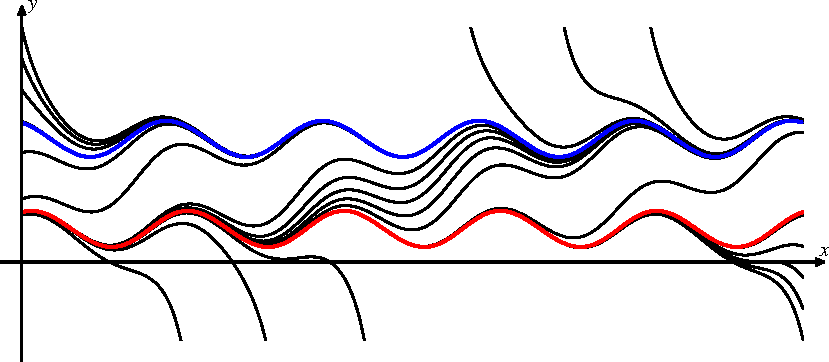
\includegraphics{chapters/images/geometrie-13.pdf}
\caption{Entwicklung des Systems~(\ref{geometrie:harvest-equation})
mit $a=5$ und $h=0.8$
\label{geometrie:harvest-graph}}
\end{figure}%
Ein eindimensionales System k"onnen wir schreiben als
\[
y'=f(x,y).
\]
Die L"osungskurven dieses Systems k"onnen wir in einem $x$-$y$-Diagramm
als Graphen darstellen.
Zum Beispiel k"onnen wir die Entwicklung des Systems
\begin{equation}
y' = ay(1-y)-h(1+\sin 2\pi x)
\label{geometrie:harvest-equation}
\end{equation}
wie in Abbildung~\ref{geometrie:harvest-graph} darstellen.
Dieses nicht-autonome System hat zwei Grenzzyklen: 
Anfangswerte oberhalb der roten Kurve f"uhren zu L"osungskurven, die
sich f"ur zunehmendes $x$ der blauen Kurve ann"ahern.
Anfangswerte unterhalb der blauen Kurve f"uhren zu L"osungskurven, die
sich f"ur abnehmendes $x$ der roten Kurve n"ahern.

Startwerte in der N"ahe der roten Kurve sind nicht stabil,
die Entwicklung f"ur zunehmende $x$ f"uhrt den Wert immer weiter von
der roten Kurve weg.
Lag der Startwert unterhalb der roten Kurve, wird die L"osung gegen
$-\infty$ divergieren.
Alle anderen L"osungen konvergieren gegen die blaue Kurve.

Offenbar ist es ziemlich schwierig, das
System~(\ref{geometrie:harvest-equation}) "uber gr"ossere $x$-Intervalle
zu verstehen. 
Zum Beispiel h"angt das Verhalten davon ab, ob der Startwert zwischen den
farbigen Kurven liegt oder ausserhalb, und diese h"angt vom Start-$x$ ab.

In Kapitel~\ref{chapter:grundlagen} wurde beschrieben, wie jedes
Differentialgleichungssystem, m"oglicherweise nach Erweiterung um eine
explizite Zeitkoordinate, zu einem autonomen System gemacht und damit
durch ein Vektorfeld ersetzt werden kann,
und wie die L"osungen als Bahnen eines Teilchens in einem zeitlich
unver"anderlichen Vektorfelde verstanden werden k"onnen.
Daraus ergibt sich auch, dass das Verhalten der L"osungen einer
Differentialgleichungen studiert werden kann, ohne dass man
die Abh"angigkeit von $x$ im Detail kennt.
Die Bahnen zerlegen den Raum und k"onnen sich nicht schneiden,
so schr"ankt die Geometrie des Raumes die M"oglichkeiten f"ur das
Verhalten der L"osung "uber lange Zeiten ein.
Besonders ausgepr"agt sind diese Einschr"ankungen im zweidimensionalen
Raum.
Eine geschlossene Kurve in der Ebene unterteilt diese in zwei Bereiche,
keine L"osung kann vom einen Bereich in den anderen f"uhren.

Ein Parameter in der Differentialgleichung modifiziert das Vektorfeld,
und kann damit Eigenschaften von L"osungen "uber lange Zeiten ver"andern.
Zum Beispiel k"onnen periodische Bahnen sich aufl"osen und zu Spiralbahnen
werden.

Wir gehen in diesem Kapitel immer von einem autonomen System
\[
\frac{d}{dx}y(x)=f(y),
\]
wobei das Vektorfeld $f(y)$ nicht von $x$ abh"angt.
Uns interessieren die geometrische Eigenschaften der L"osungskurven, 
soweit sie sich direkt aus den Eigenschaften des Vektorfeldes ableiten
lassen.
Insbesondere interessieren uns also spezielle Punkte des Vektorfeldes,
zum Beispiel Nullstellen.


%
% Spezielle Punkte und Bahnen
%
\section{Spezielle Punkte und Bahnen}
\rhead{Spezielle Punkte und Bahnen}
Das Verhalten der L"osungskurven "uber lange Zeiten wird wesentlich
beeinflusst von Punkten, in denen die Bewegung auf der Bahn
zum Stillstand kommt oder sogar die Richtung umkehrt, und von Punkten,
in die ein Punkt periodisch zur"uckkehrt.

%
% Kritische Punkte
%
\subsection{Kritische Punkte}
Wir betrachten zun"achst einen Punkt $y_0$ in dem $f(y_0)\ne 0$.
Dann gilt $f(y)\ne 0$ auch f"ur Punkte $y$, die gen"ugend nahe an 
$y_0$ sind.
Eine L"osungskurve durch $y_0$ hat im Punkt $y_0$ die Tangentenrichtung
$f(y_0)$.
In einer gen"ugend kleinen Umgebung von $y_0$ werden sich verschiedene
L"osungskurven nicht schneiden.
Ein solcher Schnittpunkt w"are ein Anfangsbedingung f"ur zwei
verschiedene L"osungen, aber der Eindeutigkeitssatz f"ur die
L"osung einer Differentialgleichung sagt, dass es zu jeder 
Anfangsbedingung nur eine L"osung geben kann.
Dies bedeutet, dass in einer Umgebung des Punktes $y_0$ nichts
Spannendes passiert, die Bahnen sehen ungef"ahr aus wie in
Abbildung~\ref{geometrie:parallelebahnen}.
\begin{figure}
\centering
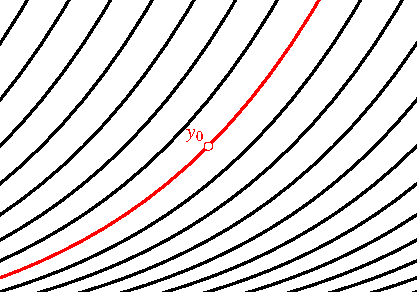
\includegraphics{chapters/images/geometrie-12.pdf}
\caption{Verlauf der Bahnen eines autonomen Differentialgleichungssystems
in der N"ahe eines Punktes $y_0$ mit $f(y_0)\ne 0$.
\label{geometrie:parallelebahnen}}
\end{figure}

Von besonderem Interesse sind daher Punkte, in denen das Vektorfeld
verschwindet:

\begin{definition}
$y$ heisst {\em kritischer Punkt} des Vektorfeldes $f$, wenn $f(y)=0$.
\end{definition}

Dass in einem kritischen Punkt das Vektorfeld verschwindet bedeutet nicht,
dass die Bahn nicht dar"uber hinweg fortgesetzt werden kann,
wie das folgende Beispiel zeigt.

\begin{beispiel}
Das eindimensionale Gleichungssystem
\[
y'=\sqrt{|y|}
\]
hat einen kritischen Punkt bei $y=0$.
Die Funktion
\begin{equation}
y(x)=\frac14x^2\operatorname{sign}(x)
\label{geometrie:1dimkritloesung}
\end{equation}
ist eine L"osungsfunktion, denn
\begin{align*}
y'(x)&=\frac12|x|\\
\sqrt{\left|\frac14x^2\operatorname{sign}(x)\right|}
&=
\sqrt{\frac14x^2}
=
\frac12|x|=y'(x).
\end{align*}
Trotzdem erreicht $y(x)$ jeden beliebigen Punkt der $y$-Achse, denn 
\[
x=2\sqrt{|y|}\operatorname{sign}(y)
\]
ist die Umkehrfunktion von $y(x)$. 
Die L"osungskurve bewegt sich also "uber den kritischen Punkt hinweg.
\begin{figure}
\centering
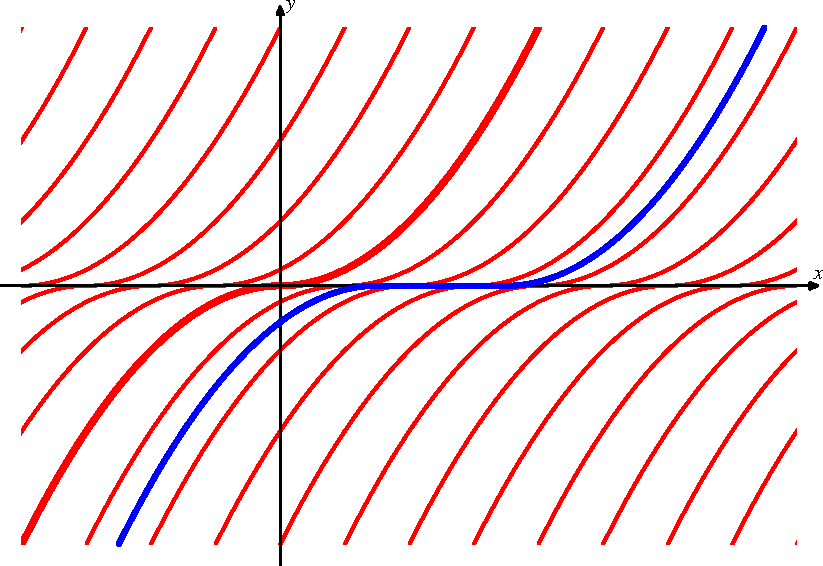
\includegraphics{chapters/images/geometrie-1.pdf}
\caption{Bahnen das Differentialgleichungssystems $y'=\sqrt{|y|}$
k"onnen den kritischen Punkt bei $y=0$ traversieren.
Die L"osung~(\ref{geometrie:1dimkritloesung}) ist etwas fetter rot
eingezeichnet.
L"osungen k"onnen aber auch beliebig lange im Punkt $y$ verweilen,
wie die blaue Kurve illustriert.
\label{geometrie:1dimkrit}}
\end{figure}
Abbildung~\ref{geometrie:1dimkrit} zeigt die Bahnen.
Die L"osung~(\ref{geometrie:1dimkritloesung}) ist nicht die einzige.
Andere L"osungen bestehen jeweils aus einem Ast der Kurve mit positiven
$y$ und einem mit negativen $y$, dazwischen kann die L"osung beliebig lange
im kritischen Punkt verweilen.
F"ur den Punkt $y=0$ ist also der Eindeutigkeitssatz verletzt, zur
Anfangsbedingung $y=0$ gibt es beliebig viele L"osungen.
\end{beispiel}

%
% Linearisierung
%
\subsection{Linearisierung}
In einem kritischen Punkt $y_0$ verschwinden alle Komponenten von $f(y_0)$.
Falls $f$ stetig differenzierbar ist, k"onnen wird $f$ in einer Umgebung
des kritischen Punktes in erster Ordnung mit Hilfe der Ableitung
approximieren:
\[
f(y)=\frac{\partial f}{\partial y}(y-y_0) + o(|y-y_0|)
\]
Die partielle Ableitung bezeichnet im mehrdimensionalen Fall
die Jacobi-Matrix, sie ist die $n\times n$-Matrix bestehend aus allen
partiellen Ableitungen der Komponenten von $f$ nach den Variablen $y_i$.
In einer Umgebung eines kritischen Punktes ist die Gestalt der Bahnen also
im wesentlichen durch die Jacobi-Matrix bestimmt.

\begin{beispiel}
Wir betrachten als Beispiel die eindimensionale ($n=1$) Differentialgleichung
\[
y'=f(y)=y,
\]
die in $y_0=0$ einen kritischen Punkt hat.
Die Jacobi-Matrix ist konstant: $f'(y)=1$.
L"osungskurven mit Anfangsbedingungen $>0$ werden daher anwachsen,
w"ahrend L"osungskurven mit Anfangsbedingungen $<0$ abnehmen werden.
Die L"osungskurven werden daher vom kritischen Punkt ``abgestossen''.

W"ahlen wir stattdessen das System
\[
y'=f(y)=-y,
\]
dann ist die Jacobi-Matrix $f'(y)=-1$, und wir k"onnen analog schliessen,
dass L"osungskurven immer zum kritischen Punkt hinstreben.
\end{beispiel}

\begin{beispiel}
Das Beispiel im letzten Abschnitt verwendet
\[
y'=f(y)=\sqrt{|y|}
\]
ist im kritischen Punkt $y=0$ nicht stetig differenzierbar, daher ist
eine lineare Approximation nicht m"oglich.
Das fr"uher beobachtete Verhalten, dass sich L"osungskurven auf der
einen Seite vom kritischen Punkt entfernen, auf der anderen aber ann"ahern,
kann nur auftreten, wenn auch $f'(0)=0$ gilt, so dass wir $f$ in zweiter
Ordnung als
\[
y'=f(y)=\frac12 f''(0)y^2.
\]
Diese Differentialgleichung hat die Funktion
\[
y(x)=-\frac{2}{f''(0)x+C}
\]
als L"osung.
Je nach Wert von $C$ bekommen wir eine L"osung, f"ur $x>0$ anwachsen
oder abfallen, wenigstens f"ur ein kleines Intervall.
Die L"osung n"ahert sich dem kritischen Punkt, oder entfernt sich, je
nachdem auf welcher Seite die L"osungskurve beginnt.
\end{beispiel}

%
% Eindimensionale Systeme
%
\section{Eindimensionale Systeme}
\rhead{Eindimensionale Systeme}
Wir untersuchen in diesem Abschnitt das Verhalten eindimensionaler autonomer
Systeme, und konzentrieren uns dabei auf Eigenschaften, die allein
auf Grund der geringen Dimension erschliessen lassen.
Ein solches System hat die Form
\[
y'=f(y),\quad y\in\mathbb R
\]
und kann sofort mit Hilfe von Separation der Variablen gel"ost werden:
\[
\int\frac{dy}{f(y)} = t+C,
\]
was nat"urlich nur funktioniert, wenn $f$ konstantes Vorzeichen hat.
Daraus folgt, dass ein Startwert $y_0$, f"ur den $f(y_0)>0$ ist,
zu einer monoton wachsenden L"osung f"uhrt, w"ahrend $f(y_0)<0$
bedeutet, dass die L"osung monoton f"allt.
Erf"ullt ein Startwert $f(y_0)=0$, dann ist $y(x)=y_0$ eine
L"osung der Differentialgleichung.
Die kritischen Punkte von $f$ strukturieren also wie erwartet die
L"osungsmenge.
Wir suchen eine "ubersichtliche Visualisierung dieser Beobachtung
und wollen verstehen, wie sich die Struktur in Abh"angigkeit
von einem Parameter in der Differentialgleichung ver"andern kann.

%
% Mögliche Phasendiagramme in einer Dimension
%
\subsection{Phasenportraits}
Seien jetzt $y_1,y_2,\dots$ Nullstellen der Funktion $f(y)$.
Dann sind die Funktion $y(x)=y_i$ L"osungen der Differentialgleichung
$y'=f(y)$.
Die Bewegung zwischen den Nullstellen wird vollst"andig dominiert durch
das Vorzeichen von $f(y)$ zwischen den Nullstellen.
Wir k"onnen dies in einem sogenannten Phasen-Portrait visualisieren.
Abbildung~\ref{geometrie:phasenportrait} zeigt die L"osungen der
Differentialgleichung
\begin{equation}
y'=f(y)=y^3-y
\label{geometrie:cube}
\end{equation}
Die Nullstellen dieser Funktion sind $-1$, $0$ und $1$.
\begin{figure}
\centering
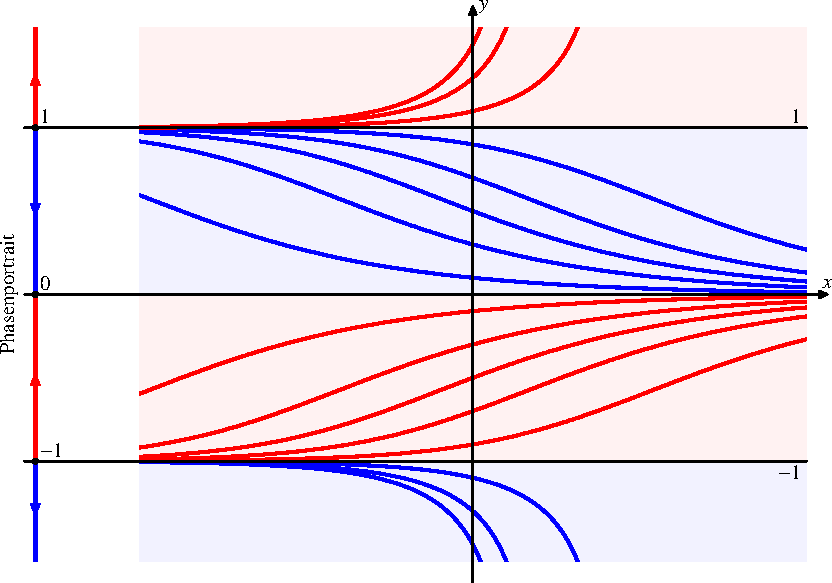
\includegraphics{chapters/images/geometrie-14.pdf}
\caption{Fluss der Differentialgleichung~(\ref{geometrie:cube}) und
Phasenportrait
\label{geometrie:phasenportrait}}
\end{figure}
Die exakte Abh"angigkeit von $x$ ist oft nicht wichtig, entscheidend
ist nur die Tatsache, dass Punkte im blauen Gebiet sich mit zunehmendem
$x$ nach unten bewegen, w"ahrend Punkte im roten Gebiet sich nach
oben bewegen.
Diese Information wird auch durch das Phasenportrait am linken
Rand der Abbildung~\ref{geometrie:phasenportrait} dargestellt.
Der Vortail eines Phasenportraits gegen"uber der Darstellung
der L"osung ist, dass sie mit einer Dimension auskommt.

%
% Mögliche Änderungen (Bifurkationen) der Phasendiagramme
%
\subsection{Bifurkationen\label{geometrie:subsection:bifurkationen}}
Betrachten wir jetzt eine Differentialgleichung, die ausserdem von einem
Parameter $b$ abh"angt:
\[
y'=f(y,b).
\]
Das Phasenportrait wird sich ver"andern, wenn $b$ variert, wir
m"ochten die verschiedenen dabei m"oglichen "Uberg"ange verstehen
k"onnen.
Es interessiert vor allem kleine "Anderungen in der Umgebung eines
Wertes $b_0$.
Dabei kommt es vor allem darauf an, dass mit Nullstellen passiert, und
welches Vorzeichen $f$ links und rechts von der Nullstelle hat.
Wir gehen daher davon aus, dass $f$ f"ur $b_0$ an der Stelle $y=0$
hat, dass also $a_0(b_0)=0$ ist.

Wenn $a_1(b_0)\ne0$ ist, also wenn $f'(0, b_0)\ne 0$ ist, dann 
gilt dies auch in einer Umgebung von $b_0$, und daher wird die
Nullstelle in erster N"aherung nur verschoben:
\[
y_0(b) \simeq -\frac{f(0,b)}{f'(0,b)},
\]
Das Phasenportrait erlebt also keine grundds"atzlichen "Anderung.

\subsubsection{Sattel-Knoten-Bifurkation}
Wir betrachten jetzt den Fall $f(0,b_0)=0$ und $f'(0,b_0)=0$, die Funktion
$f$ ist f"ur $b=b_0$ quadratisch, mit einer Nullstelle im Scheitel.
Variert $b$, wird zwar der Graph von $y\mapsto f(y,b)$ seine
Gestalt "andern, aber er wird weiterhin "ahnlich wie eine Parabel
aussehen.
Etwas interessantes passiert nur, wenn der Scheitel von die horizontale
Achse "uberquert, wenn also beim Durchgang von $b$ durch den Wert $b_0$
die Zahl der Nullstellen von $0$ auf $2$ steigt oder umgekehrt.
Dies bedeutet, dass 
\[
f''(y_0,b_0)\ne 0
\qquad
\text{und}
\qquad
\frac{\partial f}{\partial b}(y_0, b_0)\ne 0.
\]
Modellhaft k"onnen wir dies durch das System
\[
f(y,b)=y^2+b
\]
wiedergeben.
Es hat f"ur $b<0$ die Nullstellen $\pm\sqrt{-b}$, f"ur $b>0$ jedoch
keine Nullstellen.
Das zugeh"orige Phasenportrait ist in Abbildung~\ref{geometrie:saddle-node}
dargestellt.
Bei dieser Art von Bifurkation entstehen neue kritische Punkte
paarweise, davon ist jeweils einer stabil, der andere instabil.
Diese Art der Bifurkation heisst {\em Sattel-Knoten-}
oder {\em Saddle-Node-Bifurkation}.
\index{Sattel-Knoten-Bifurkation}
\index{Saddle-Node-Bifurkation}

\begin{figure}
\centering
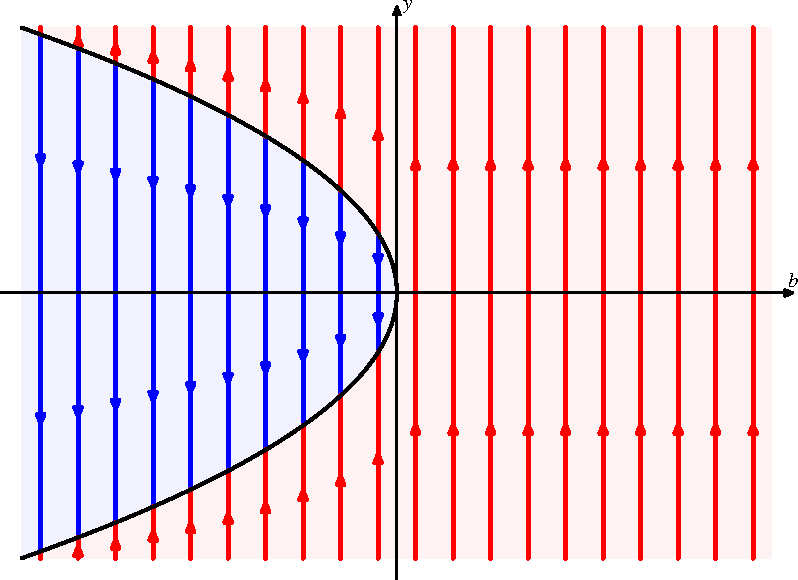
\includegraphics{chapters/images/bifurkation-1.pdf}
\caption{Phasendiagramm f"ur die Sattel-Knoten-Bifurkation in
Abh"angigkeit vom Parameter $b$.
\label{geometrie:saddle-node}}
\end{figure}

\subsubsection{Heugabel-Bifurkation}
\begin{figure}
\centering
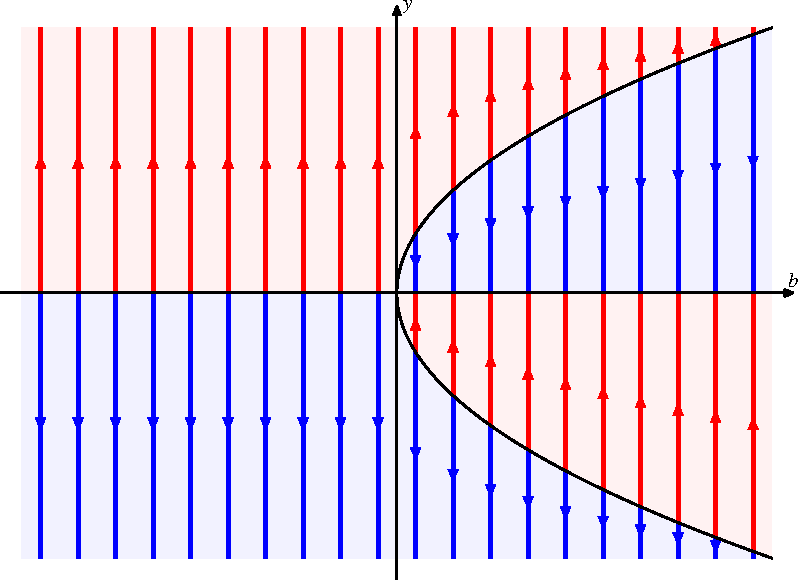
\includegraphics{chapters/images/bifurkation-2.pdf}
\caption{Phasendiagramm f"ur die Heugabel-Bifurkation in Abh"angigkeit vom
Parameter $b$.
\label{geometrie:pitchfork}}
\end{figure}
Eine andere Art von Bifurkatione zeigt das Modell
\[
f(y,b)=y^3-by.
\]
F"ur $b<0$ hat die Funktion $y\mapsto f(y,b)$ nur die eine
reelle Nullstelle $y=0$.
F"ur $b>0$ dagegen liegen die drei verschiedenen Nullstellen
$-\sqrt{b}$, $0$  und $\sqrt{b}$.
Das zugeh"orige Phasendiagramm ist in Abbildung~\ref{geometrie:pitchfork}
dargestellt, diese Art von Bifurkation heisst {\em Heugabel-}
oder {\em Pitchformk-Bifurkation}.
\index{Heugabel-Bifurkation}
\index{Pitchfork-Bifurkation}
Bei dieser Art von Bifurkation werden aus einer Nullstelle deren drei.
War die Nullstelle instabil (wie in Abbildung~\ref{geometrie:pitchfork}),
entstehen zwei neue instabile Nullstellen, die bisherige Nullstellen 
wird stabil.
War die eine Nullstelle stabil, entstehen zwei stabile Nullstellen, die
eine Nullstelle wird instabil.

\subsubsection{Transkritische Bifurkation}
\begin{figure}
\centering
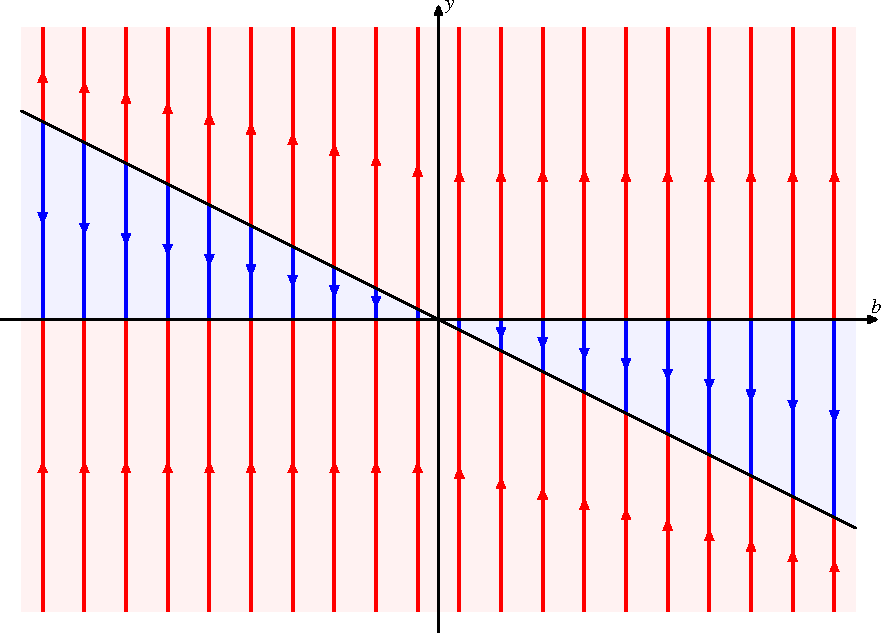
\includegraphics[width=\hsize]{chapters/images/bifurkation-3.pdf}
\caption{Phasendigramm f"ur die transkritische Bifurkation in Abh"angigkeit
vom Parameter $b$.
\label{geometrie:transkritisch}}
\end{figure}
Das Standard-Modell f"ur die sogenannten {\em transkritische Bifurkation} ist 
\index{transkritische Bifurkation}
\[
f(y,b)=y^2+yb = y(y+b)
\]
(Abbildung~\ref{geometrie:transkritisch}).
F"ur $b=0$ hat dieses System einen kritischen Punkt bei $y=0$.
Eine L"osungskurve, die bei negativem $y$ beginnt, wird immer n"aher
an den Punkt $y=0$ herankommen.
Liegt der Anfangswert jedoch im Gebiet $y>0$, wird sich die L"osungskurve
immer weiter von $y=0$ entfernen.
Der Fixpunkt bei $y=0$ ist also weder stabil noch instabil.

F"ur $b\ne 0$ entsteht ein weiterer kritischer Punkt bei $y=-b$.
Da f"ur $y\to\pm\infty$ die Funktion $y\mapsto f(y,b)$ immer positiv
ist, ist der rechte der beiden Fixpunkte immer stabil, der
linke immer instabil.


%
% Zweidimensionale Systeme
%
\section{Zweidimensionale Systeme}
\rhead{Zweidimensionale Systeme}
In diesem Abschnitt betrachten wir die geometrischen Einschr"ankungen, denen
zweidimensionale autonome Systeme unterliegen.
Wieder sind Punkte von besonderem Interesse, in denen $f$ verschwindet.
Bei eindimensionalen Systemen teilen solche Punkte den $y$-Bereich in
verschiedene Intervall, in denen die Bewegung nur in jeweils
eine Richtung erfolgen kann, damit ist es leicht zu entscheiden,
ob ein solcher kritischer Punkt stabil oder instabil ist.
In zwei Dimensionen legen die Punkte alleine den Charakter noch nicht
fest, insbesondere ist es ja auch m"oglich, dass eine Bahn einen solche
Punkt umschliesst.

\subsection{Nullklinen}
Kritische Punkte von $f$ sind solche, in denen beide Komponenten
des Vektors $f(y)$ verschwinden.
Die Gleichungen
\[
f_1(y)=0
\qquad\text{und}\qquad
f_2(y)=0
\]
beschreiben zwei Kurvenscharen in der Ebene, die sogenannten 
{\em Nullklinen}.
\index{Nullkline}
Die Schnittpunkte von Nullklinen sind die kritischen Punkte.

Da auf einer Nullkline jeweils eine der Komponenten von $f(y)$ verschwindet,
schneiden L"osungskurven Nullklinen immer entweder horizontal oder
vertikal.
Ausserdem trennen die Nullklinen Gebiete unterschiedlicher Bewegungsrichtung
entlang einer Achse. 
Die Nullkline $f_1(y)=0$ trennt Gebiete, in denen sich eine L"osungskurve
nach rechts (zu gr"osseren $y_1$ hin) bewegt ($f_1(y)>0$) von Gebieten,
in denen sich die L"osungskurve nach links ($f_1(y)<0$) bewegt.
Desgleichen trennt die Nullkline $f_2(y)=0$ Gebiete mit Bewegung ``nach oben''
von Gebieten mit Bewegung ``nach unten''.
Allein aus dieser Information kann man sich bereits ein recht gutes
qualitives Bild "uber den Verlauf der L"osungen verschaffen, wie wir
im Folgenden an zwei Beispiel illustrieren wollen.

\begin{beispiel}
\begin{figure}
\centering
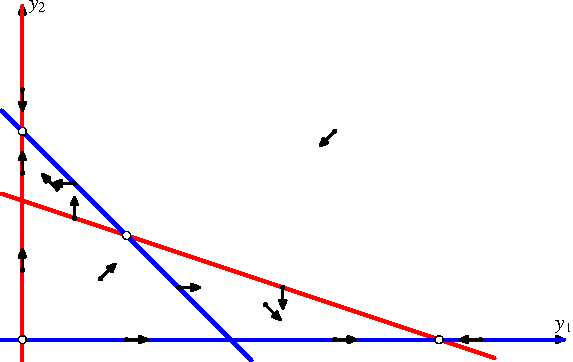
\includegraphics{chapters/images/nullklinen-1.pdf}
\caption{Nullklinen der Differentialgleichung~(\ref{geometrie:nullklinen-dgl1}),
die $y_1$-Nullklinen in rot, die $y_2$-Nullklinen in blau.
Kritische Punkte sind die Schnittpunkte verschiedenfarbiger Nullklinen.
\label{geometrie:nullklinen1}}
\end{figure}
\begin{figure}
\centering
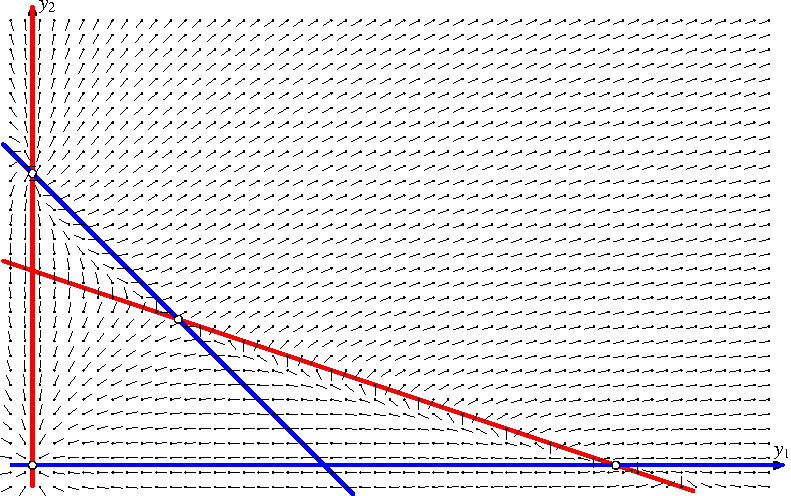
\includegraphics{chapters/images/nullklinen-2.pdf}
\caption{Vektorfeld der Differentialgleichung~(\ref{geometrie:nullklinen-dgl1}),
es best"atigt die Resultate der qualitiativen Diskussion aus
Abbildung~\ref{geometrie:nullklinen1}.
\label{geometrie:nullklinen-fluss}}
\end{figure}
\begin{figure}
\centering
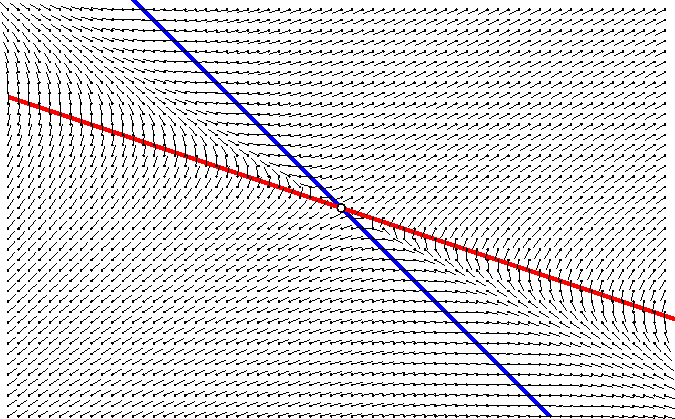
\includegraphics{chapters/images/nullklinen-3.pdf}
\caption{Vektorfeld der Differentialgleichung~(\ref{geometrie:nullklinen-dgl1})
in einer Umgebung des instabilen kritischen Punktes $(\frac12,\frac12)$.
\label{geometrie:nullklinen-instabil}}
\end{figure}
\begin{figure}
\centering
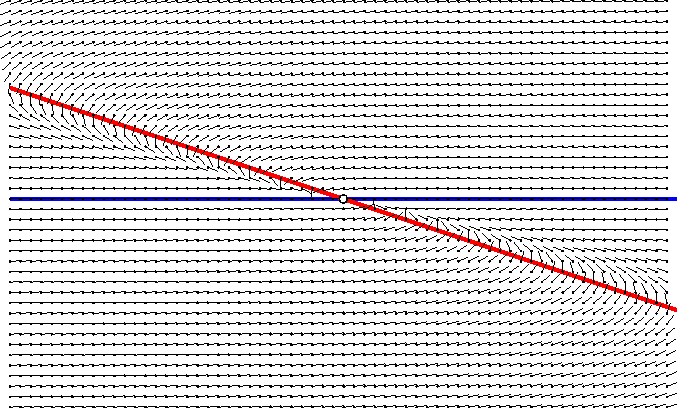
\includegraphics{chapters/images/nullklinen-4.pdf}
\caption{Vektorfeld der Differentialgleichung~(\ref{geometrie:nullklinen-dgl1})
in einer Umgebung des stabilen kritischen Punktes $(2,0)$.
\label{geometrie:nullklinen-stabil}}
\end{figure}
Wir betrachten das nichtlineare System 
\begin{equation}
\frac{d}{dx} \begin{pmatrix}y_1\\y_2\end{pmatrix}
=
\begin{pmatrix}
2y_1\biggl(1-\displaystyle\frac{y_1}2\biggr)-3y_1y_2\\
y_2(1-y_2)-y_1y_2
\end{pmatrix}.
\label{geometrie:nullklinen-dgl1}
\end{equation}
Die direkte L"osung ist ziemlich aussichtslos, wir versuchen daher mit
Hilfe der Nullklinen ein qualitatives Bild
(Abbildung~\ref{geometrie:nullklinen1}) zu erhalten.

Die $y_2$-Nullkline hat die Gleichung
\[
0=y_2(1-y_2)-y_1y_2=y_2(1-y_2-y_1)
\qquad\Rightarrow\qquad
y_2=0
\quad\text{oder}\quad
y_1+y_2=1.
\]
L"osungskurven schneiden also die beiden Geraden $y_2=0$ (die $y_1$-Achse)
und $y_1+y_2=1$ horizontal.
Da die $y_1$-Achse bereits horizontal ist, bedeutet dies, dass sich die
L"osungskurven der $y_1$-Achse anschmiegen.

Die $y_1$-Nullkline hat die Gleichung
\[
0=2y_1\biggl(1-\frac{y_1}2\biggr)-3y_1y_2=y_1(2-y_1-3y_2),
\qquad\Rightarrow\qquad
y_1=0
\quad\text{oder}\quad
y_1+3y_2=2.
\]
Wir schliessen wieder, dass die L"osungskurven die $y_2$-Achse und
die Gerade $y_1+3y_2=3$ vertikal schneiden.
Da die $y_2$-Achse schon vertikal ist, m"ussen sich auch dort
die L"osungskurven anschmiegen.

Wir k"onnen aus den Nullklinen auch die kritischen Punkte ableiten.
Da sind zun"achst die Punkte auf den Achsen, also zum Beispiel
der Schnittpunkt der $y_2$-Nullkline $y_2=0$ mit der $y_1$-Nullkline
$y_1+3y_2=2$, also $(2,0)$, oder der Schnittpunkt der
$y_1$-Nullkline $y_1=0$ mit der $y_2$-Nullkline $y_1+y_2=0$, also $(0,1)$.
Ausserdem ist nat"urlich $(0,0)$ ein kritischer Punkt.
ein vierter kritischer Punkt entsteht als Schnittpunkt
der $y_1$-Nullkline $y_1+3y_2=2$ mit der $y_2$-Nullkline $y_1+y_2=1$,
also als L"osung des linearen Gleichungssystems
\[
\begin{linsys}{2}
y_1&+&3y_2&=&2\phantom{.}\\
y_1&+& y_2&=&1,
\end{linsys}
\]
es hat die L"osung $(\frac12,\frac12)$.
Die kritischen Punkte sind also
\begin{equation}
(0,0),\quad
(2,0),\quad
(0,1)\quad\text{und}\quad
\biggl(\frac12,\frac12\biggr).
\label{geometrie:nullklinen-krit}
\end{equation}

An den aus den Nullklinen l"asst sich auch die Bewegungsrichtung der
L"osungen im Bezug auf die kritischen Punkte ablesen.
\label{geometrie:nullklinen-stabilitaet}
Aus dem Gebiet oben rechts und unten links in der N"ahe des Ursprungs
bewegen sich die L"osungen zun"achst auf den kritischen Punkt
bei $(\frac12,\frac12)$ zu, weichen dann aber ab in Richtung auf die
kritischen Punkte $(0,1)$ und $(2,0)$ zu.
Die kritischen Punkte $(0,0)$ und $(\frac12,\frac12)$ sind also
instabil, w"ahrend $(2,0)$ und $(0,1)$ stabil sind.
Dies wird auch von dem genaueren Vektorfeld in
Abbildung~\ref{geometrie:nullklinen-fluss} best"atigt.
In Abschnitt~\ref{geometrie:umgebung-kritisch} wird gezeigt, dass man 
die Bewegung in der Umgebung eines kritischen Punktes mit Hilfe der
Eigenwerte der Ableitungen klassifizieren kann.
\end{beispiel}


\begin{beispiel}
Das {\em Fitzhugh-Nagumo-Modell} wird verwendet, um das Verhalten eines Neurons
zu simulieren.
\index{Fitzhugh-Nagumo-Modell}
\begin{figure}
\centering
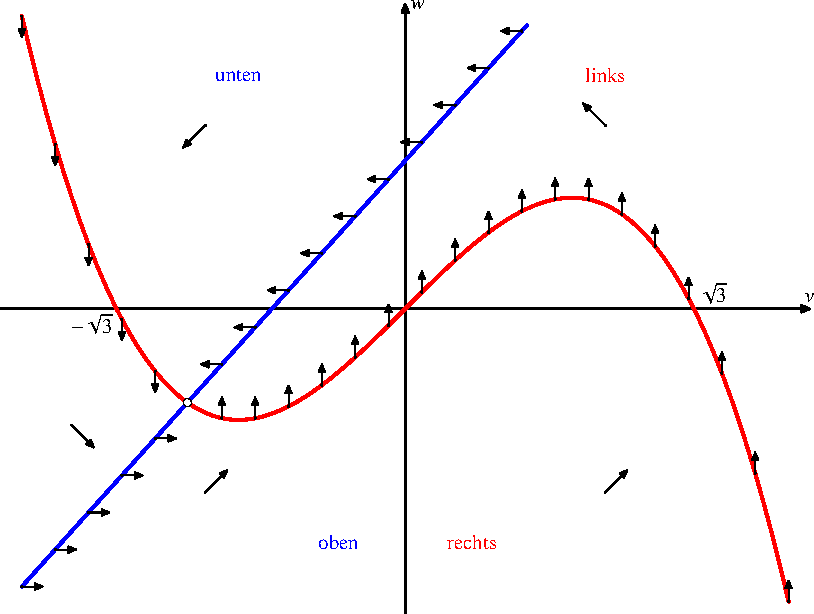
\includegraphics{chapters/images/nullklinen-5.pdf}
\caption{Nullklinen des Fitzhugh-Nagumo-Modells bei nur einem kritischen Punkt,
$a=-0.8$, $b=0.9$.
\label{geometrie:nullklinen-fh-1}}
\end{figure}
\begin{figure}
\centering
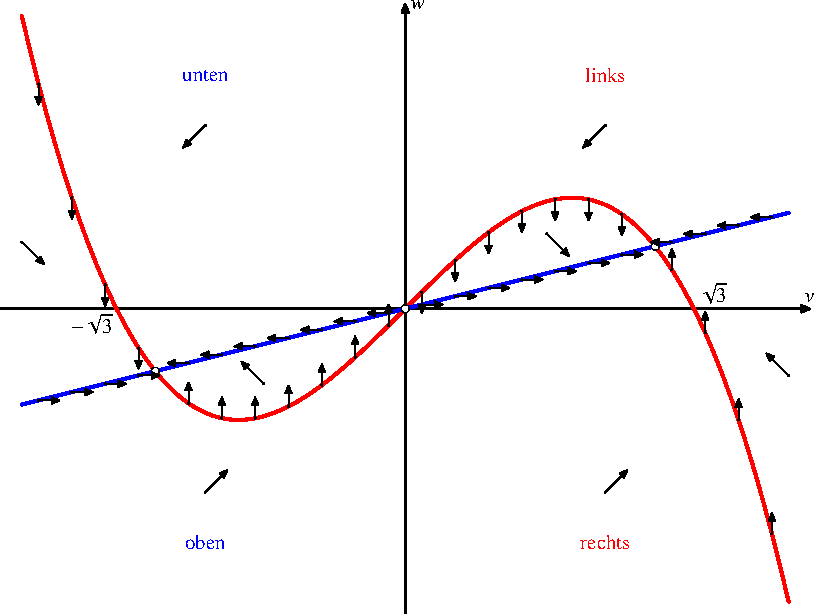
\includegraphics{chapters/images/nullklinen-6.pdf}
\caption{Nullklinen des Fitzhugh-Nagumo-Modells mit drei kritischen Punkten,
$b=4$, $a=0$.
\label{geometrie:nullklinen-fh-2}}
\end{figure}
Es verwendet das Differentialgleichungssystem
\begin{equation}
\begin{aligned}
    \dot v&= v-\frac13v^3-w\\
\tau\dot w&= v-a-bw.
\end{aligned}
\label{geometrie:fitzhugh-dgl}
\end{equation}
Wir versuchen, uns wieder mit Hilfe der Nullklinen ein Bild von den
L"osungskurven zu verschaffen.
Die $v$-Nullkline hat die Gleichung
\[
0=v-\frac13v^3-w
\qquad\Rightarrow\qquad
w=v-\frac13v^3 = v(1-{\textstyle\frac1{\sqrt{3}}}v)(1+{\textstyle\frac1{\sqrt{3}}}v)
\]
Diese kubische Parabel hat im Nullpunkt die Steigung $1$.
Die $w$-Nullkline ist die Gerade
\[
0=v-a-bw
\qquad\Rightarrow\qquad
v=bw+a
\qquad\Rightarrow\qquad
w = \frac{v-a}{b}.
\]
Wenn die Steigung $1/b$ dieser Geraden gr"osser als $1$ ist, dann schneidet
die Gerade die kubische Parabel nur in einem Punkt, es gibt dann nur
einen kritischen Punkt.
Ist die Steigung $1/b<1$, gibt es f"ur nicht zu grosses $|a|$ drei
Schnittpunkte.

In Abbildung~\ref{geometrie:nullklinen-fh-1} sind die Nullklinen des
Fitzhugh-Nagumo-Modells mit nur einem kritischen Punkt dargestellt.
Die L"osungskurven bewegen sich in Spiralen im Gegenurzeigersinn
um den Fixpunkt herum.
In diesem Fall erlauben die Nullklinen keine abschliessende Beurteilung
der Stabilit"at des Fixpunktes.
Die Untersuchung der Eigenwerte der Jacobi-Matrix, die im nächsten
Abschnitt erkl"art wird, erm"oglicht die Entscheidung, und wird in
der Fortsetzung dieses Beispiels auf Seite~\pageref{geometrie:fh-fortsetzung}
durchgef"uhrt.

In Abbildung~\ref{geometrie:nullklinen-fh-2} sind die Nullklinen des
Fitzhugh-Nagumo-Modells dargstellt mit drei kritschen Punkten.
Man kann sofort ablesen, dass $(0,0)$ ein instabiler kritischer Punkt ist.
Die L"osungskurven, die von diesem Punkt abgestossen werden, n"ahern sich
einem der beiden anderen kritischen Punkte und bewegen sich
in einer Spirale um diesen Punkt herum.
Da sich die L"osungskurven nicht schneiden d"urfen kann man folgern,
dass die beiden anderen kritschen Punkte stabil sein m"ussen,
die L"osungskurven werden sich ihnen in Spiralbahnen n"ahern.
\label{geometrie:fh-diskussion}
\end{beispiel}

%
% Bewegung in der Umgebung eines kritischen Punktes
%
\subsection{Bewegung in der Umgebung eines kritischen Punktes
\label{geometrie:umgebung-kritisch}}
Wir gehen jetzt davon aus, dass 
\[
y'=f(y)
\]
einen kritischen Punkt hat, wir k"onnen die Koordinaten immer so w"ahlen,
dass der kritische Punkt im Nullpunkt des Koordinatensystems liegt.
Die Bewegung in unmittelbarer Umgebung des Nullpunktes kann dann approximiert
werden durch die Bewegung des linearisierten Systems
\[
y'=\frac{\partial f(0)}{\partial y}y
\]
Die m"oglichen Bewegungsformen in der Umgebung des kritischen Punktes
sind also bestimmt durch die Jacobi-Matrix.
Jede beliebige $2\times 2$-Matrix kann auch tats"achlich als Jacobi-Matrix
vorkommen, denn das System
$
y'=Ay
$
hat die Matrix $A$ als Jacobi-Matrix.

Wir interessieren uns im Moment nur f"ur eine qualitative Beschreibung
der L"osungen, wir k"onnen also immer eine Koordinatentransformation
vornehmen, um die Situation zu vereinfachen.
Die gesuchte qualitative Klassifizierung von zweidimensionalen
Differentialgleichungssystemen l"auft also auf eine Klassifizierung
von reellen $2\times 2$-Matrizen bis auf Koordinatentransformation
hinaus.

Eine solche Klassifikation kann auf der Basis von Eigenwerten und
Eigenvektoren erfolgen.
Dazu ben"otigen wir eine "Ubersicht "uber die Eigenwerte einer
Matrix
\[
A=\begin{pmatrix}a&b\\c&d\end{pmatrix},
\]
die wir als Nullstellen des charakteristischen Polynoms bestimmen
k"onnen.
Das charakteristische Polynom ist
\[
\chi_A(\lambda)
=
\det(A-\lambda E)
=
\left|\,\begin{matrix}a-\lambda&b\\c&d-\lambda\end{matrix}\,\right|
=
(a-\lambda)(d-\lambda)-bc
=
\lambda^2-(a+b)\lambda + ad-bc,
\]
es ist bestimmt durch die Spur und die Determinante der Matrix
\[
\begin{aligned}
\det A&=ad -bc,
&
\operatorname{Spur}A&=a+d
&
&\Rightarrow
&
\chi_A(\lambda)&=\lambda^2-\lambda \operatorname{Spur}A+\det A
\end{aligned}
\]
Die L"osungsformel f"ur die quadratische Gleichung liefert die
Eigenwerte
\[
\lambda_{1,2}
=
\frac{\operatorname{Spur}A}2\pm\sqrt{\Delta}
\qquad
\qquad
\text{mit}\quad
\Delta = \biggl(\frac{\operatorname{Spur}A}2\biggr)^2 - \det A
\]
Falls die Diskriminanten $\Delta > 0$ ist, sind die beiden Eigenwerte
verschieden, und folglich gibt es zwei verschiedene Eigenvektoren,
die Matrix $A$ kann diagonalisiert werden mit Diagonalelementen
$\lambda_{1,2}$.  Das Differentialgleichungssystem zerf"allt dann
in zwei unabh"angige eindimensionale Systeme
\begin{align*}
y_1'&= \lambda_1 y_1\\
y_2'&= \lambda_2 y_2,
\end{align*}
die auch durch
\begin{align*}
y_1(x)&=y_{10} e^{\lambda_1 x}\\
y_2(x)&=y_{20} e^{\lambda_2 x}
\end{align*}
sofort gel"ost werden k"onnen.
F"ur die Diskussion der Form der L"osungskurven brauchen wir aber die
Abh"angigkeit der beiden Koordinaten untereinander, nicht von $x$.
Wir stellen daher $y_2$ als Funktion von $y_1$ dar:
\[
y_1=y_{10} e^{\lambda_1 x}
\qquad\Rightarrow\qquad
x=\frac1{\lambda_1}\log\frac{y_1}{y_{10}}
\qquad\Rightarrow\qquad
y_2
=
y_{20} e^{\frac{\lambda_2}{\lambda_1}\log\frac{y_1}{y_{10}}}
=
y_{20}\biggl(\frac{y_1}{y_{10}}\biggr)^{\frac{\lambda_2}{\lambda_1}}
=
Cy^{\frac{\lambda_2}{\lambda_1}}
\]
\begin{figure}
\centering
\begin{tabular}{ccc}
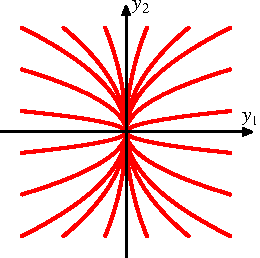
\includegraphics{chapters/images/geometrie-2.pdf}&%
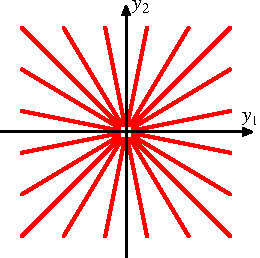
\includegraphics{chapters/images/geometrie-3.pdf}&%
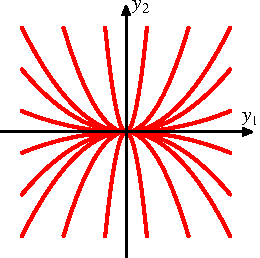
\includegraphics{chapters/images/geometrie-4.pdf}\\
$\displaystyle \frac{\lambda_2}{\lambda_1}>1$&%
$\displaystyle \frac{\lambda_2}{\lambda_1}=1$&%
$\displaystyle \frac{\lambda_2}{\lambda_1}<1$
\end{tabular}
\caption{L"osungskurven des linearisierten Systems f"ur
$\frac{\lambda_2}{\lambda_1}>0$.
\label{geometrie:posportraits}}
\end{figure}

\begin{figure}
\centering
\begin{tabular}{ccc}
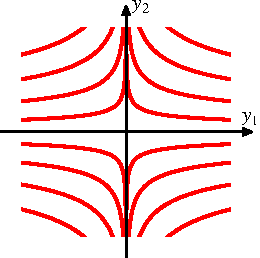
\includegraphics{chapters/images/geometrie-5.pdf}&%
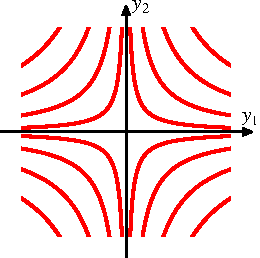
\includegraphics{chapters/images/geometrie-6.pdf}&%
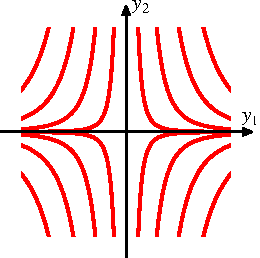
\includegraphics{chapters/images/geometrie-7.pdf}\\
$\displaystyle \frac{\lambda_2}{\lambda_1}>-1$&%
$\displaystyle \frac{\lambda_2}{\lambda_1}=-1$&%
$\displaystyle \frac{\lambda_2}{\lambda_1}<-1$
\end{tabular}
\caption{L"osungskurven des linearisierten Systems f"ur
$\frac{\lambda_2}{\lambda_1}<0$.
\label{geometrie:negportraits}}
\end{figure}
Die Gestalt der L"osungskurven sind also im Wesentlichen durch den
Quotienten $\lambda_2/\lambda_1$ bestimmt.
Die Abbildung~\ref{geometrie:posportraits} zeigt die L"osungskurven
f"ur positive Werte des Quotienten, w"ahrend
Abbildung~\ref{geometrie:negportraits} die L"osungskurven f"ur
negative Werte des Quotienten zeigt.
F"ur positive Werte von $\lambda_2/\lambda_1$ bewegen sich die 
Punkte entweder immer auf den kritischen Punkt zu, oder entfernen
sich.
F"ur negative Werte von $\lambda_2/\lambda_1$ n"ahert sich ein
Punkt in der N"ahe der einen Achse zun"achst immer mehr dem kritischen
Punkt, um sich dann in Richtung der anderen Achse zu entfernen.

Die Matrix $A$ muss jedoch nicht diagonalisierbar sein, wenn
$\lambda_1=\lambda_2$.
Wenn die Matrix nur einen Eigenvektor hat, dann kann die Matrix
durch eine geeignete Koordinatentransformation in die Form
\[
\begin{pmatrix}
\lambda&      1\\
      0&\lambda
\end{pmatrix}
\]
bringen.
Die Differentialgleichungen lauten in diese Fall
\begin{align*}
y_1'&=\lambda y_1 + y_2\\
y_2'&=\lambda y_2
\end{align*}
Die zweite Gleichung kann wie vorher gel"ost werden, die L"osung f"ur $y_2$
ist
\[
y_2(x)=y_{20}e^{\lambda x},
\]
dies k"onnen wir in die erste Gleichung einsetzen, sie lautet jetzt
\[
y_1' = \lambda y_1 + y_{20}e^{\lambda x},
\]
dies ist wieder eine lineare Differentialgleichung, diesmal jedoch
eine inhomogene. 
Die L"osung der homogenen Gleichung ist $Ce^{\lambda x}$, die L"osung
der inhomogenen Gleichung kann durch Variation der Konstanten gefunden
werden, also $y_1(x)=C(x)e^{\lambda x}$.
Setzen wir dies in die Differentialgleichung 
\[
y_1'(x)
=
C'(x)e^{\lambda x}+C(x)\lambda e^{\lambda x}
=
\lambda y_1(x) + C'(x)e^{\lambda x}
=
\lambda y_1(x) + y_{20}e^{\lambda x}
\]
ein.
Diese Gleichung kann nur erf"ullt sein, wenn
\[
C'(x)=y_{20}
\qquad\Rightarrow\qquad
C(x)=y_{20}x+y_{10},
\]
die L"osung der Gleichung ist also
\[
y(x)=\begin{pmatrix}
y_{20}x+y_{10}\\
y_{20}
\end{pmatrix}e^{\lambda x}.
\]
\begin{figure}
\centering
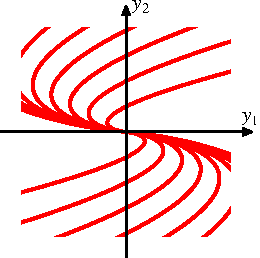
\includegraphics{chapters/images/geometrie-8.pdf}
\caption{L"osungskurven f"ur den Fall nicht diagonalisierbarer Jacobi-Matrix
mit zwei gleichen Eigenwerten.
\label{geometrie:jnf-kurven}}
\end{figure}%
In Abbildung~\ref{geometrie:jnf-kurven} sind die L"osungskurven dargestellt.
F"ur $\lambda >0$ streben die L"osungskurven gegen den Nullpunkt, aber auf
eine Art, sie im Grenzfall die $y_1$-Achse ber"uhren.

Falls die Diskriminante $\Delta$ negativ ist, gibt es keine reellen
Eigenwerte, also auch keine reellen Eigenvektoren.
Wir k"onnen aber trotzdem eine Basis finden, in der die Geometrie
dar Bahnkurven leichter verst"andlich ist.
Dazu schreiben wir 
\[
\alpha = \frac{\operatorname{Spur}A}2=\frac{a+d}2
\qquad
\text{und}
\qquad
\beta = \sqrt{-\Delta},
\]
und betrachten die beiden Vektoren
\[
w_1 = \begin{pmatrix}0\\\beta\end{pmatrix}.
\qquad\text{und}\qquad
w_2 = \begin{pmatrix}b\\\alpha-a\end{pmatrix}
\]
Wir berechnen die Wirkung der Matrix $A$ auf diesen beiden Vektoren,
und zerlegen jeweils das Resultat wieder in $w_1$ und $w_2$:
\begin{align*}
Aw_1
&=
\begin{pmatrix}a&b\\c&d\end{pmatrix}
\begin{pmatrix}0\\\beta\end{pmatrix}
=
\begin{pmatrix}
\beta b\\
\beta d
\end{pmatrix}
=
v
\begin{pmatrix}0\\\beta\end{pmatrix}
+
\beta
\begin{pmatrix}b\\\alpha-a\end{pmatrix}
\\
Aw_2
&=
\begin{pmatrix}a&b\\c&d\end{pmatrix}
\begin{pmatrix}b\\\alpha-a\end{pmatrix}
=
\begin{pmatrix}
ab-ab+b\alpha\\
bc-ad+\alpha d
\end{pmatrix}
=
\alpha
\begin{pmatrix}b\\\alpha-a\end{pmatrix}
+u
\begin{pmatrix}0\\\beta\end{pmatrix}
\end{align*}
Wir m"ussen nur noch die Konstanten $u$ und $v$ bestimmen:
\begin{align*}
\beta d
&=
v\beta
+
\alpha\beta
-
\beta a
&&\Rightarrow&
v
&=
\alpha a+d-\alpha=2\alpha-\alpha=\alpha
\\
-\det A +\alpha d
&=
\alpha^2- \alpha a+u\beta
&&\Rightarrow&
u\beta&=-\det A +\alpha(a+d)-\alpha^2
=\alpha^2-\det A
=\Delta=-\beta^2
\end{align*}
Aus der zweiten Gleichung folgt $ u=-\beta$.
Damit haben wir die Wirkung der Matrix $A$ auf den Vektoren $w_1$ und $w_2$
bestimmt, und wir k"onnen daraus die Matrix von $A$ in der Basis
$\{w_1,w_2\}$ ablesen, wir bezeichnen sie mit $A'$
\[
\begin{aligned}
Aw_1&=\alpha w_1 + \beta w_2\\
Aw_2&=-\beta w_1 + \alpha w_2
\end{aligned}
\qquad\Rightarrow\qquad
A'=\begin{pmatrix}
\alpha&\beta\\
-\beta&\alpha
\end{pmatrix}
\]
Dies ist die gesuchte Form der Matrix, in der sich die L"osungskurven
leichter beschreiben lassen.
Eine L"osung daf"ur l"asst sich angeben, wenn man ber"ucksichtigt, dass
$A'$ einer Drehmatrix "ahnelt.
Wir vermuten daher, dass die L"osungskurve im wesentlichen den kritischen
Punkt umkreist, m"oglicherweise mit einer "Anderung des Abstandes
zum kritischen Punkt, und schreiben daher
\begin{equation}
y(x)
=
\begin{pmatrix}
r_0e^{ux}\cos(vx+\delta_0)\\
r_0e^{ux}\sin(vx+\delta_0)
\end{pmatrix}
=
r_0e^{ux}
\begin{pmatrix}
\cos(vx+\delta_0)\\
\sin(vx+\delta_0)
\end{pmatrix}
,
\label{geometrie:rotsol}
\end{equation}
wobei wird $r_0$ und $\delta_0$ so w"ahlen, dass
\[
y_{10}=r_0\cos\delta_0
\qquad\text{und}\qquad
y_{20}=r_0\sin\delta_0.
\]
Setzen wir jetzt den Ansatz~(\ref{geometrie:rotsol}) in die
Differentialgleichung ein, erhalten wir
\begin{align*}
y'(x)
&=
\begin{pmatrix}
r_0ue^{ux}\cos(vx+\delta_0)-r_0e^{ux}v\sin(vx+\delta_0)\\
r_0ue^{ux}\sin(vx+\delta_0)+r_0e^{ux}v\cos(vx+\delta_0)
\end{pmatrix}
\\
&=
\begin{pmatrix}
 \alpha&\beta\\
-\beta &\alpha
\end{pmatrix}
\begin{pmatrix}
r_0e^{ux}\cos(vx+\delta_0)\\
r_0e^{ux}\sin(vx+\delta_0)
\end{pmatrix}
=
\begin{pmatrix}
r_0e^{ux}\alpha\cos(vx+\delta_0)+r_0e^{ux}\beta\sin(vx +\delta_0)\\
-r_0e^{ux}\beta\cos(vx+\delta_0)+r_0e^{ux}\alpha\sin(vx+\delta_0)
\end{pmatrix}
\end{align*}
Diese Gleichung ist genau dann korrekt, wenn 
\[
u=\alpha
\qquad\text{und}\qquad
v=-\beta.
\]
Die Zahlen $\alpha$ und $\beta$ charakterisieren also wieder die L"osung.
F"ur $\alpha < 0$ n"ahern sich die L"osungen dem kritischen Punkt, f"ur
$\alpha>0$ entfernen sie sich.
Die Zahl $\beta$ ist die Winkelgeschwindigkeit, mit der die L"osung
um den kritischen Punkt rotiert.
Die L"osungskurven sind daher Spiralen um den kritischen Punkt, sie
sind in Abbildung~\ref{geometrie:rotkurv} dargestellt.
\begin{figure}
\centering
\begin{tabular}{ccc}
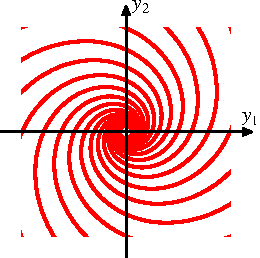
\includegraphics{chapters/images/geometrie-9.pdf}&%
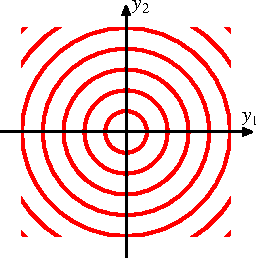
\includegraphics{chapters/images/geometrie-11.pdf}&%
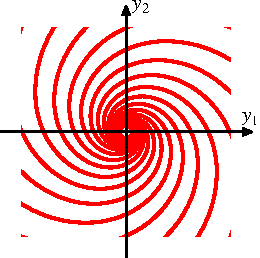
\includegraphics{chapters/images/geometrie-10.pdf}\\
$\alpha > 0$&$\alpha = 0$&$\alpha < 0$
\end{tabular}
\caption{L"osungskurven des linearisierten Systems im Falle $\Delta < 0$
sind Spiralen um den kritischen Punkt
\label{geometrie:rotkurv}}
\end{figure}

\begin{beispiel}
Wir kehren nochmals zum Beispiel~(\ref{geometrie:nullklinen-dgl1})
von Seite~\pageref{geometrie:nullklinen-dgl1} zur"uck.
Die kritischen Punkte wurden in (\ref{geometrie:nullklinen-krit}) bereits
zusammengestellt.
Die Ableitung von $f$, also die Jacobi-Matrix, ist
\[
\frac{\partial f}{\partial y}
=
\frac{\partial}{\partial y}
\begin{pmatrix}
2y_1-y_1^2-3y_1y_2\\
y_2-y_2^2-y_1y_2
\end{pmatrix}
=
\begin{pmatrix}
2-2y_1-3y_2 & -3y_1\\
-y_2        &1-2y_2-y_1
\end{pmatrix}
\]
In den vier kritischen Punkten finden wir die folgenden Matrizen und
Eigenwerte
\begin{align*}
&(0,0)
	&\frac{\partial f}{\partial y}&=\begin{pmatrix}2&0\\0&1\end{pmatrix}
		&&\lambda_1=2,\;\lambda_2=1\\
&(2,0)
	&\frac{\partial f}{\partial y}&=\begin{pmatrix}-2&-6\\0&-1\end{pmatrix}
		&&\lambda_1=-2,\;\lambda_2=-1\\
&(0,1)
	&\frac{\partial f}{\partial y}&=\begin{pmatrix}-1&0\\-1&-1\end{pmatrix}
		&&\lambda_1=-1,\;\lambda_2=-1\\
&\textstyle(\frac12,\frac12)
	&\frac{\partial f}{\partial y}&=\begin{pmatrix}-\frac12&-\frac32\\-\frac12&-\frac12\end{pmatrix}
		&&\lambda_1=\frac{\sqrt{3}-1}2,\;\lambda_2=-\frac{\sqrt{3}+1}2
\end{align*}
Nur bei den Punktein $(2,0)$ und $(0,1)$ sind beide Eigenwerte negativ,
nur diese beiden Punkte sind stabil, wie bereits die  Diskussion der
Nullklinen auf Seite~\pageref{geometrie:nullklinen-stabilitaet}
gezeigt hat.
\end{beispiel}

%
% Komplexe Eigenwerte
%
\subsection{Komplexe Eigenwerte}
Die Darstellung im vorangegangenen Abschnitt war darum bem"uht,
komplexe Zahlen zu vermeiden.
Die Darstellung im Falle $\Delta<0$ wurde dadurch unn"otig verkompliziert,
in diesem Abschnitt soll gezeigt werden, wie die Formeln f"ur die Vektoren
$w_1$ und $w_2$ mit Hilfe komplexer Zahlen hergeleitet werden k"onnen.

Zun"achst halten wir fest, dass im Falle $\Delta<0$ zwei konjugiert
komplexe Eigenwerte
$
\lambda= \alpha + i\beta
$
und
$
\overline{\lambda}= \alpha - i\beta
$
existieren.
Nehmen wir an, dass $v$ ein Eigenvektor zum Eigenwert $\lambda$ ist,
dann ist $\overline{v}$, dessen Komponenten die konjugiert komplexen
Komponenten von $v$ sind, ein Eigenvektor zum Eigenwert $\overline{\lambda}$.
Grund daf"ur ist die Tatsache, dass die Matrix $A$ nur reelle Matrixelemente
hat, also gilt
\[
A\overline{v}
=
\overline{Av}
=
\overline{\lambda v}=\overline{\lambda}\overline{v}.
\]
Der Vektor $v$ ist nat"urlich nicht geeignet f"ur eine reelle Beschreibung
der L"osungskurven des linearisierten Systems.
Wir konstruieren daher die Vektoren
\begin{equation}
\begin{aligned}
w_1&=\frac{i}2(v-\overline v)
&&\qquad
&
v&=-iw_1+w_2
\\
w_2&=\frac12(v+\overline v)
&&\qquad
&
\overline{v}&=iw_1+w_2
\end{aligned}
\label{geometrie:wv}
\end{equation}
und untersuchen, wie die Matrix $A$ darauf wirkt:
\begin{align*}
Aw_1
&=
\frac{i}2(Av-A\overline v)
=
\frac{i}2(\lambda v-\overline{\lambda}\overline{v})
\\
Aw_2
&=
\frac12(Av+A\overline{v})
=
\frac12(\lambda v+\overline{\lambda}\overline{v}).
\end{align*}
Setzen wir die Darstellungen von $v$ und $\overline{v}$ durch $w_i$ aus 
(\ref{geometrie:wv}) ein, und erhalten:
\begin{align*}
\frac{i}2(\lambda v-\overline{\lambda}\overline{v})
&=
\frac{i}2(\lambda(-iw_1+w_2) -\overline{\lambda}(iw_1+w_2))
=
\frac{1}2(\lambda+\overline{\lambda}) w_1
+
\frac{i}2(\lambda-\overline{\lambda}) w_2
=\alpha w_1-\beta w_2
\\
\frac12(\lambda v+\overline{\lambda}\overline{v})
&=
\frac12(\lambda(-iw_1+w_2)+\overline{\lambda}(iw_1+w_2))
=
-\frac{i}2(\lambda-\overline{\lambda}) w_1
+
\frac12(\lambda+\overline{\lambda}) w_2.
=\beta w_1+\alpha w_2
\end{align*}
Verwendet man also $\{w_1,w_2\}$ als Basis, dann bekommt die Matrix die
Form
\begin{equation}
A'=\begin{pmatrix}
\alpha&-\beta\\
\beta &\alpha
\end{pmatrix}
\label{geometrie:drehmatrix}
\end{equation}
Auf Grund der Konstruktion haben die Vektoren $w_1$ und $w_2$ reelle
Komponenten, $w_1$ ist der Realteil des Vektors $v$, $w_2$ ist
der Imagin"arteil.
Damit haben wir ein Rezept, wie wir eine Basis von reellen Vektoren
konstruieren k"onnen, in denen das System die
Form~(\ref{geometrie:drehmatrix}) hat.

Die Komponenten eines Eigenvektors $v$ erf"ullen die Gleichung
\[
(a-\lambda)v_1 + bv_2=0
\]
eine L"osung daf"ur ist
\[
v=\begin{pmatrix}
-b\\
a-\alpha-i\beta
\end{pmatrix},
\]
dessen Real- und Imagin"arteile
\[
\begin{pmatrix}
-b\\a-\alpha
\end{pmatrix}
\qquad\text{und}\qquad
\begin{pmatrix}
0\\\beta
\end{pmatrix},
\]
dies sind die Vektoren, die im vorangegangenen Abschnitt aus dem "Armel
gesch"uttelt worden waren, um die Matrix des Systems in die
Form~(\ref{geometrie:drehmatrix}) zu bringen.

\begin{beispiel}
\label{geometrie:fh-fortsetzung}
Wir wenden obige Analyse auf das
Fitzhugh-Nagumo-Modell~(\ref{geometrie:fitzhugh-dgl}) von
Seite~\pageref{geometrie:fitzhugh-dgl} an.
Um die Diskussion etwas zu vereinfachen, untersuchen wir nur den Fall
$\tau = 1$.
Wir m"ussen die Jacobi-Matrix in einem kritischen Punkt bestimmen, sie ist
\begin{equation}
J=
\begin{pmatrix}
1-v^2 &  -1 \\
  1   &  -b
\end{pmatrix}.
\end{equation}
Das charakteristische Polynom ist
\begin{align*}
\det(J-\lambda E)
&=
\left|
\begin{matrix}
1-v^2-\lambda&-1\\
1&-b-\lambda
\end{matrix}
\right|
\\
&=
(1-v^2-\lambda)(-b-\lambda)+1
\\
&=
(\lambda+v^2-1)(\lambda+b)+1
\\
&=
\lambda^2 + (\underbrace{v^2 + b - 1}_{\textstyle p})\lambda
+ \underbrace{b(v^2 - 1)+1}_{\textstyle q}.
\end{align*}
Es hat die Nullstellen
\begin{equation}
\lambda_{1,2}
=
-\frac{p}{2}\pm\sqrt{\frac{p^2}4-q}
=
-\frac{v^2+b-1}2\pm\sqrt{\frac{(v^2+b-1)^2}4-b(v^2-1)-1}.
\label{geometrie:fn-eigenwerte}
\end{equation}
Der erste Term in der Wurzel ist das Quadrat des Terms vor der Wurzel.
Ohne $q$ in der Wurzel g"abe es einen Eigenwert mit dem gleichen Vorzeichen
wie $p$, der andere ist $0$.
Die Vorzeichen von $p$ und $q$ bestimmen also weitgehen, ob ein 
kritischer Punkt stabil oder instabil ist.

\begin{enumerate}
\item
Wenn $q<0$ ist, dann ist die Wurzel gr"osser als $p/2$, die beiden
Eigenwerte haben verschiedenes Vorzeichen, und der kritische Punkt
ist instabil unabh"angig vom Vorzeichen von $p$. 
Dieser Fall tritt ein, wenn 
\[
b(v^2 -1) + 1 < 0
\qquad\Rightarrow\qquad
1-\frac1b > v^2.
\]
F"ur $b<1$ wird die linke Seite negativ, dann kann dieser Fall also gar nicht
eintreten.
\item
Ist $q>0$ und von gen"ugend grossem absolutem Betrag,
dann wird der Radikand negativ, beide Eigenwerte
sind komplex und der kritische Punkt ist genau dann stabil, wenn $p>0$ ist.
Ist $q>0$, aber nicht von gen"ugend grossem absolutem Betrag, dann
bleibt der Radikand positiv.
In diesem Fall haben beide Eigenwerte das gleiche Vorzeichen wie $p$,
auch in diesem Fall hat man also Stabilit"at genau dann, wenn $p>0$ ist.
\end{enumerate}
Wir k"onnen die Resultate der obigen Diskussion in der folgenden
Entscheidungstabelle zusammenfassen:
\begin{center}
\begin{tabular}{|>{$}c<{$}|>{$}c<{$}|l|}
\hline
q=b(v^2-1)+1 & p= v^2 + b -1 &           \\
\hline
     <0      &               &  instabil \\
     >0      &       <0      &  instabil \\
     >0      &       >0      &  stabil   \\
\hline
\end{tabular}
\end{center}

F"ur $b>1$ und $a=0$ ist $(0,0)$ ein kritischer Punkt, und es gilt $q=-b+1<0$
und $p=b-1>0$, wir sind daher im Fall~1, der Ursprung ist instabil.
Es ist aber auch $p=v^2+b-1>v^2\ge 0$, der Fall $p<0$ kann also 
gar nicht eintreten, ein solcher kritischer Punkt muss also immer
stabil sein.
Dies deckt sich mit den Resultaten der Diskussion von
Seite~\pageref{geometrie:fh-diskussion}.
\end{beispiel}

%
% Hopf-Bifurkation
%
\subsection{Hopf-Bifurkation}
\begin{figure}
\centering
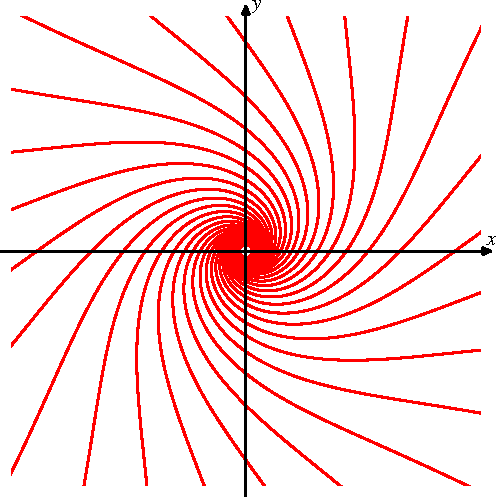
\includegraphics{chapters/images/hopf-1.pdf}
\caption{Fluss f"ur $b<0$, der kritische Punkt ist stabil,
Bahnkurven konvergieren gegen $0$.
\label{geometrie:hopf1}}
\end{figure}%
\begin{figure}
\centering
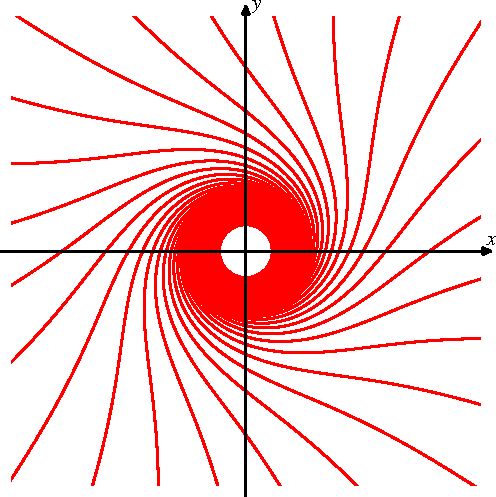
\includegraphics{chapters/images/hopf-2.pdf}
\caption{Fluss f"ur $b=0$, der kritische Punkt ist immer noch stabil,
die Bahnkurven n"ahern sich jedoch nicht mehr exponentiell schnell
dem Nullpunkt.
\label{geometrie:hopf2}}
\end{figure}%
\begin{figure}
\centering
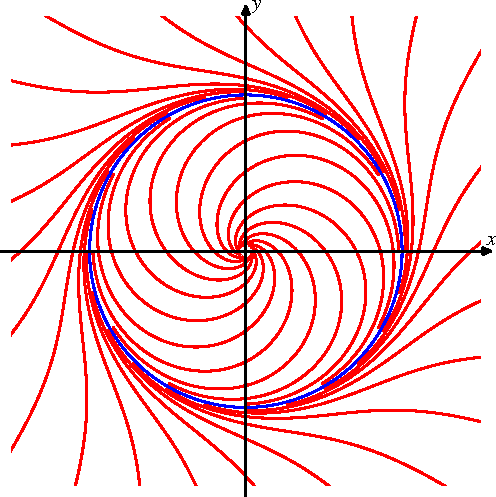
\includegraphics{chapters/images/hopf-3.pdf}
\caption{Fluss f"ur $b>0$, der Nullpunkt ist nicht mehr stabil, daf"ur
ist der Kreis mit Radius $\sqrt{b}$ eine stabile periodische Bahn (blau),
gegen die alle Bahnkurven exponentiell schnell konvergieren.
\label{geometrie:hopf3}}
\end{figure}%
\begin{figure}
\centering
\begin{tabular}{ccc}
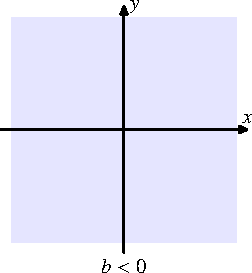
\includegraphics{chapters/images/hopf-4.pdf}&%
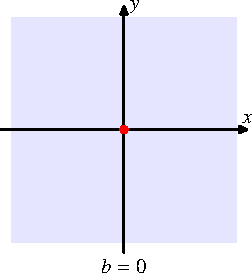
\includegraphics{chapters/images/hopf-5.pdf}&%
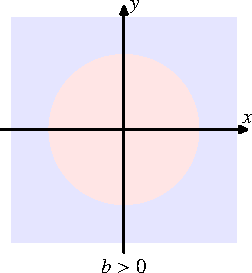
\includegraphics{chapters/images/hopf-6.pdf}%
\end{tabular}
\caption{Vorzeichen von $\dot r$ in Abh"angigkeit von $b$.
Punkte mit $\dot r <0$ sind blau gef"arbt, Punkte mit $\dot r >0$ rot.
\label{geometrie:hopfvorzeichen}}
\end{figure}%
Die in Abschnitt~\ref{geometrie:subsection:bifurkationen} untersuchten
Bifurkationen eindimensionaler Differentialgleichungen k"onnen in
analoger Form auch bei zweidimensionalen Differentialgleichungen auftreten.
Sie sind jedoch immer eindimensionale Bifurkationen, die entlang der
durch die Eigenvektoren der Linearisierung gegebenen Richtungen
auftreten.

Die h"ohere Dimensionszahl erlaubt aber auch eine Bifurkation, bei der
ein stabiler Fixpunkt in stabil wird und einen stabilen Zyklus ``abwirft''
(Abbildungen~\ref{geometrie:hopf1}, \ref{geometrie:hopf2} and
\ref{geometrie:hopf3}).
Sie heisst die Hopf-Bifurkation.
\index{Hopf-Bifurkation}
Wir betrachten dazu das System 
\begin{equation}
\begin{aligned}
\dot r      &= r(b-r^2)\\
\dot \varphi&= -1
\end{aligned}
\label{geometrie:hopfsystem}
\end{equation}
in Polarkoordinaten.
Offenbar ist $r=0$ ein Fixpunkt.
F"ur $b>0$ gibt es ausserdem eine periodische Bahn mit $r=\sqrt{b}$
(Abbildung~\ref{geometrie:hopf3}).
Wir wollen die Stabilit"at des Fixpunktes sowie der periodischen Bahn
untersuchen.
Die Abbildung~\ref{geometrie:hopfvorzeichen} fasst die f"ur das Bahnverhalten
entscheidenden Vorzeichen in den drei F"allen $b<0$, $b=0$ und $b>0$
zusammen.

In Polarkoordinaten beschreibt die Gleichung f"ur $r$ eine
Heugabel-Bifurkation.
Der kritische Punkt $r$ ist f"ur $b<0$ stabil, er wird f"ur $b>0$
instabil, daf"ur entstehen zwei neue stabile kritische Punkte
$r=\pm\sqrt{b}$.

Unsere bisherige Theorie zur Beurteilung von Fixpunkten ging von
kartesischen Koordinaten aus, wir f"uhren daher die Analyse auch noch
in kartesischen Koordinaten durch.
Die Umrechnungsformeln von Polarkoordinaten in kartesische Koordinaten
und ihre Ableitungen
\[
\begin{aligned}
x&=r\cos\varphi&&\qquad&\dot x&=\dot r\cos\varphi-r\sin\varphi\cdot\dot\varphi\\
y&=r\sin\varphi&&\qquad&\dot y&=\dot r\sin\varphi+r\cos\varphi\cdot\dot\varphi
\end{aligned}
\]
erlauben uns,
das System~(\ref{geometrie:hopfsystem}) in kartesische Koordinaten
umzurechnen:
\begin{equation}
\begin{aligned}
\dot x&=r(b-r^2)\frac{x}{r}+y=(b-x^2-y^2)x+y\\
\dot y&=r(b-r^2)\frac{y}{r}-x=(b-x^2-y^2)y-x.
\end{aligned}
\label{geometrie:hopf-kartesisch}
\end{equation}
Zur Beurteilung der Stabilit"at des Nullpunktes berechnen wir die
Jacobi-Matrix
\[
J(x,y)=
\begin{pmatrix}
b-3x^2-y^2&1-2xy\\
-1-2xy&b-x^2-3y^2
\end{pmatrix}
\quad\Rightarrow\quad
J(0,0)=\begin{pmatrix}
b&1\\-1&b
\end{pmatrix}.
\]
Die Matrix $J(0,0)$ hat das charakteristische Polynom
\[
(b-\lambda)^2+1=0
\]
mit den Nullstellen
\[
\lambda=b\mp i.
\]
Stabilit"at wird durch das Vorzeichen des Realteils der Eigenwerte
bestimmt, wir lesen daher ab, dass der kritische Punkt $0$ stabil
ist f"ur $b<0$ und instabil f"ur $b>0$.

\section{"Ubungsaufgaben}
\rhead{"Ubungsaufgaben}
\begin{uebungsaufgaben}
\item
\input uebungsaufgaben/601.tex
\item
\input uebungsaufgaben/602.tex
\item
\input uebungsaufgaben/603.tex
\end{uebungsaufgaben}

%
% komplex.tex -- Komplexe Differentialgleichungen
%
% (c) 2015 Prof Dr Andreas Mueller, Hochschule Rapperswil
%
\chapter{Komplexe Differentialgleichungen\label{chapter:komplexeanalysis}}
\lhead{}
\rhead{Komplexe Differentialgleichungen}
Die bisher betrachteten Differentialgleichungen waren immer f"ur
$x\in\mathbb R$ definiert.
Bei der L"osung mit Hilfe von Potenzreihen haben wir L"osungsfunktionen
gefunden, die man auch f"ur komplexe $x$-Werte auswerten kann.
Definiert man die Ableitung einer Funktionen einer komplexen Variablen
$z$ rein formal als
\[
\frac{d}{dz}z^n= nz^{n-1},
\]
dann kann man auch Potenzreihen in der Variablen $z$ formal differenzieren,
indem man jeden Term der Potenzreihe ableitet.
Und die mit der Potenzreihen-Methode gefunden L"osungen erf"ullen dann
auch die urspr"ungliche Differentialgleichung.
Dies ist aber eine rein formale "Uberlegung, da die Ableitung nach einer
komplexen Variablen noch gar nicht definiert ist.

\section{Komplex differenzierbare Funktionen}
Wir betrachten in diesem Kapitel komplexwertige Funktionen,
die ein einem Teilgebiet der komplexen Ebene definiert sind.
Ein {\em Gebiet} ist eine offene Teilmenge $\Omega\subset \mathbb C$.
{\em Offen} heisst, dass mit jedem Punkt $z_0\in\Omega$ eine Umgebung
\[
U=\{z\in\mathbb Z\,|\,|z-z_0|<\varepsilon\}
\]
ebenfalls in $\Omega$ enthalten ist, also $U\subset \Omega$ f"ur gen"ugen
kleines $\varepsilon$.
Sei also $f(z)$ eine in $\Omega\subset\mathbb C$ definierte
Funktion $f\colon\Omega\to\mathbb C$. 

Eine komplexwertige Funktion $f(z)$ kann betrachtet werden als zwei
reellwertige Funktionen von zwei Variablen $x$ und $y$:
\[
f(z)=\operatorname{Re}f(x+iy) + i \operatorname{Im}f(x+iy)
\]
Schreibt man
$\operatorname{Re}f(x+iy)=u(x,y)$
und
$\operatorname{In}f(x+iy)=v(x,y)$,
dann ist die komplexe Funktion vollst"andig durch reelle Funktionen
beschrieben.
Und nat"urlich wissen wir auch, was unter den Ableitungen der Funktionen 
$u(x,y)$ und $v(x,y)$ zu verstehen ist.
Der Funktion $f(z)$ entspricht eine Abbildung $\mathbb R^2\to\mathbb R^2$
\[
(x,y)\mapsto\begin{pmatrix}u(x,y)\\v(x,y)\end{pmatrix}.
\]
Die Ableitung einer solchen Funktion im Punkt $(x_0,y_0)$
ist eine lineare Abbildung von Vektoren, die in linearer N"aherung
den Funktionswert bei $f(z_0 + \Delta z)$ 
\[
\begin{pmatrix}
u(x+\Delta x, y +\Delta y)\\
v(x+\Delta x, y +\Delta y)
\end{pmatrix}
=
\begin{pmatrix}
\frac{\partial u}{\partial x}&\frac{\partial u}{\partial y}\\
\frac{\partial v}{\partial x}&\frac{\partial v}{\partial y}
\end{pmatrix}
\begin{pmatrix} \Delta x\\\Delta y \end{pmatrix}
+o(\Delta x, \Delta y).
\]
In dieser Sicht einer komplexen Funktion gibt es keine einzelne Zahl, die
die Funktion einer Ableitung "ubernehmen k"onnte, die Ableitung
ist eine $2\times 2$-Matrix.

\subsection{Komplexe Ableitung}
Die Ableitung einer Funktion einer reellen Variablen wird mit Hilfe des
Grenzwertes
\[
f'(x_0)=\lim_{x\to x_0}\frac{f(x)-f(x_0)}{x-x_0}
\]
definiert, oder als diejenige Zahl $f'(x_0)\in\mathbb R$ mit der Eigenschaft,
dass
\begin{equation}
f(x)=f(x_0)+f'(x_0)(x-x_0) + o(x-x_0)
\label{komplex:abldef}
\end{equation}
gilt.
Der Term $x-x_0$ und die Gleichung (\ref{komplex:abldef}) sind aber auch
f"ur komplexe Argument sinnvoll, wir definieren daher

\begin{definition}
Die komplexe Funktion $f(z)$ heisst im Punkt komplex differenzierbar
und hat die komplexe Ableitung $f'(z_0)\in\mathbb C$,
wenn 
\begin{equation}
f(z)=f(z_0) + f'(z_0)(z-z_0) +o(z-z_0)
\label{komplex:defkomplabl}
\end{equation}
gilt.
\end{definition}

\begin{beispiel}
Die Funktion $z\mapsto f(z)=z^n$ ist "uberall komplex differenzierbar
und hat die Ableitung $nz^{n-1}$.
Um dies nachzupr"ufen, m"ussen wir die Bedingung~(\ref{komplex:defkomplabl})
verifizieren.
Aus einer wohlbekannten Faktorisierung von $z^n - z_0^n$ k"onnen wir den
Differenzenquotienten finden:
\[
\frac{f(z)-f(z_0)}{z-z_0}
=
\frac{z^n-z_0^n}{z-z_0}
=
\frac{(z-z_0)(z^{n-1}+z^{n-2}z_0+z^{n-3}z_0^2+\dots+z^{n-1})}{z-z_0}
=
z^{n-1}+z^{n-2}z_0+z^{n-3}z_0^2+\dots+z^{n-1}
\]
Lassen wir jetzt $z$ gegen $z_0$ gehen, wird die rechte Seite
zu $nz_0^{n-1}$.
\end{beispiel}

\begin{beispiel}
Die Funktion $z\mapsto f(z)=\bar z=x-iy$ ist nicht differenzierbar.
Wenn $f(z)=\bar z$ differenzierbar w"are, dann m"usste es eine Zahl
$a\in\mathbb C$ geben, so dass 
\[
\bar z-\bar z_0=a(z-z_0)+o(z-z_0)
\]
gilt.
w"ahlen wir $z=z_0+x$ bzw.~$z=z_0+iy$, dann erhalten wir
\[
\begin{aligned}
z-z_0&=x:&
\bar z-\bar z_0&=x
&&\Rightarrow&
\bar z-\bar z_0&=1\cdot x
&&\Rightarrow&
a&=1
\\
z-z_0&=iy:&
\bar z-\bar z_0&=-iy
&&\Rightarrow&
\bar z-\bar z_0&=-1\cdot iy
&&\Rightarrow&
a&=-1
\end{aligned}
\]
Es ist also nicht m"oglich, eine einzige Zahl $a$ zu finden, die als
die Ableitung der Funktion $z\mapsto \bar z$ betrachtet werden k"onnte.
\end{beispiel}

Das letzte Beispiel zeigt, dass
selbst Funktionen, deren Real- und Imagin"arteil beliebig oft stetig
differenzierbare Funktionen sind, nicht komplex differenzierbar
sein m"ussen.
Komplexe Differenzierbarkeit ist eine wesentlich st"arkere Bedingung
an eine Funktion, komplex differenzierbare Funktionen bilden eine
echte Teilmenge aller Funktionen, deren Real- und Imagin"arteil
differenzierbar ist.

\subsection{Die Cauchy-Riemann-Differentialgleichungen}
Komplexe Funktionen k"onnen nur differenzierbar sein, wenn sich die vier
partiellen Ableitungen zu einer einzigen komplexen Zahl zusammenfassen
lassen.
Um diese Beziehung zu finden, gehen wir von einer komplexen Funktion
\[
f(x+iy) = u(x,y) + iv(x,y)
\]
aus, und berechnen die Ableitung auf zwei verschiedene Arten, indem
wir sowohl nach $x$ als auch nach $iy$ ableiten:
\begin{align*}
f'(z)&
=
\lim_{x\to 0}\frac{f(z+x)-f(z)}{x}
=
\frac{\partial u}{\partial x}+i\frac{\partial v}{\partial x}
\\
f'(z)&
=
\lim_{y\to 0}\frac{f(z+x)-f(z)}{iy}
=
\frac1{i}
\frac{\partial u}{\partial y}+\frac{\partial v}{\partial y}
=
\frac{\partial v}{\partial y}
-i
\frac{\partial u}{\partial y}.
\end{align*}
Dies ist nur m"oglich, wenn Real- und Imagin"arteile "ubereinstimmen.
Es folgt also

\begin{satz}
\label{komplex:satz:cauchy-riemann}
Real- und Imagin"arteil $u(x,y)$ und $v(x,y)$ einer
komplexe Funktion $f(z)$ mit $f(x+iy)=u(x,y)+iv(x,y)$
erf"ullen die Cauchy-Riemannschen Differentialgleichungen
\index{Cauchy-Riemann-Differentialgleichungen}
\begin{equation}
\begin{aligned}
\frac{\partial u}{\partial x}
&=
\frac{\partial v}{\partial y},
&
\frac{\partial u}{\partial y}
&=
-
\frac{\partial v}{\partial x}
\end{aligned}
\label{komplex:dgl:cauchy-riemann}
\end{equation}
\end{satz}

Leitet man die Cauchy-Riemann-Differentialgleichungen nochmals nach
$x$ und $y$ ab, erh"alt man
\begin{equation*}
\begin{aligned}
\frac{\partial^2 u}{\partial x^2}
&=
\frac{\partial^2 v}{\partial x\,\partial y},
&
\frac{\partial^2 u}{\partial x\,\partial y}
&=
-\frac{\partial^2 v}{\partial x^2},
&
\frac{\partial^2 u}{\partial y\,\partial x}
&=
\frac{\partial^2 v}{\partial y^2},
&
\frac{\partial^2 u}{\partial y^2}
&=
-\frac{\partial^2 v}{\partial y\,\partial x}.
\end{aligned}
\end{equation*}
Die erste und die letzte sowie die mittleren zwei k"onnen zu jeweils
einer Differentialgleichung f"ur die Funktionen $u$ und $v$ zusammengefasst
werden, n"amlich
\begin{equation*}
\frac{\partial^2 u}{\partial x^2}
+
\frac{\partial^2 u}{\partial y^2}
=
0
\qquad\text{und}\qquad
\frac{\partial^2 v}{\partial x^2}
+
\frac{\partial^2 v}{\partial y^2}
=
0
\end{equation*}

\begin{definition}
Der Operator 
\[
\Delta =
\frac{\partial^2}{\partial x^2}
+
\frac{\partial^2}{\partial y^2}
\]
heisst der {\em Laplace-Operator} in zwei Dimensionen
\index{Laplace-Operator}.
\end{definition}

\begin{definition}
Eine Funktion $h(x,y)$ von zwei Variablen heisst {\em harmonisch}, wenn sie
die Gleichung
\[
\Delta h=0
\]
erf"ullt.
\index{harmonische Funktion}
\end{definition}

\begin{satz}
Real- und Imagin"arteil einer komplexen Funktion sind harmonische Funktionen.
\end{satz}

Die Cauchy-Riemann-Differentialgleichungen schr"anken also einerseits stark
ein, welche Funktionen "uberhaupt als Real- und Imagin"arteil einer
komplex differenzierbaren Funktion in Frage kommen.
Andererseits koppeln sie auch Real- und Imagin"arteil stark zu sammen.

\begin{beispiel}
Von einer komplex differenzierbaren Funktion $f(z)$ sei nur der Realteil
$u(x,y)=x^3 -3xy^2$ bekannt.
Zun"achst kontrollieren wir, ob dies "uberhaupt ein Realteil sein kann,
indem wir nachrechnen, ob $u(x,y)$ harmonisch ist.
\begin{equation*}
\begin{aligned}
\frac{\partial u}{\partial x}
&=
3x^2-3y^2
&&\Rightarrow&
\frac{\partial^2 u}{\partial x^2}
&=
6x
\\
\frac{\partial u}{\partial y}
&=
-6xy
&&\Rightarrow&
\frac{\partial^2 u}{\partial y^2}
&=
-6x
\\
&&&&\Delta u&=\frac{\partial^2u}{\partial x^2}+\frac{\partial^2u}{\partial y^2}=6x-6x=0,
\end{aligned}
\end{equation*}
$u$ ist also harmonisch.
Um die Funktion $f$ zu finden, brauchen wir jetzt noch den Imagin"arteil.
Wir finden ihn mit Hilfe der Cauchy-Riemann-Differentialgleichungen.
Es gilt
\begin{equation}
\begin{aligned}
\frac{\partial v}{\partial x}
&=
-\frac{\partial u}{\partial y}=6xy,
&
\frac{\partial v}{\partial y}
&=
\frac{\partial u}{\partial x}=3x^2-3y^2
\end{aligned}
\label{komplex:crbeispiel}
\end{equation}
Aus der ersten Gleichung erh"alt man durch Integrieren nach $x$ 
\[
v(x,y)=-3x^2y + C(y),
\]
die Integrations-``Konstante'' ist eine Funktion, die aber nur von $y$
abh"angen darf.
Die zweite Cauchy-Riemann-Gleichung verwendet die Ableitung von $v$ nach $y$,
sie ist
\[
\frac{\partial v}{\partial y}=3x^2+C'(y).
\]
Aus der zweiten Gleichung von (\ref{komplex:crbeispiel}) liesst man
ab, dass
\[
C'(y)=-3y^2
\qquad\Rightarrow\qquad
C(y)=-y^3+k
\]
sein muss.
Damit ist $v$ bis auf eine Konstante bestimmt.
Die zugeh"orige Funktion $f(z)$ ist daher
\[
f(z)=f(x+iy)=x^3-3xy^2+i(3x^2y-y^3)+ik
=x^3 + 3x^2iy + 3x(iy)^2+(iy)^3+ik=z^3+ik.
\]
Wir haben die Funktion $f(z)$ bis auf eine Konstanten $ik$ 
aus ihrem Realteil rekonstruiert.
\end{beispiel}

\subsection{Wegintegrale und die Cauchy-Formel}
Das Finden einer Stammfunktion, die Integration, ist die Grundtechnik,
mit der man den "Ubergang von lokaler Information in Form von Ableitungen,
zu globaler Information "uber reelle Funktionen vollzieht.
Sie liefert aus der Steigung zwischen zwei Punkten $x_0$ und $x$ den
Funktionswert mittels
\[
f(x)=f(x_0)+\int_{x_0}^xf'(\xi)\,d\xi.
\]
Bei einer reellen Funktion gibt es nur eine Richtung, entlang der man
integrieren k"onnte.

Auch in der komplexen Ebene erwarten wir eine Formel
\[
f(z) = f(z_0) + \int_{z_0}^z f'(\zeta)\,d\zeta.
\]
In der komplexen Ebene gibt es aber beliebig viele Wege, mit denen die
Punkte $z_0$ und $z$ verbunden werden k"onnen. 
Der Wert von $f(z)$ muss also durch Integration entlang eines speziell
gew"ahlten Weges $\gamma$
\[
f(z) = f(z_0) + \int_{\gamma} f'(\zeta)\,d\zeta
\]
bestimmt werden.
Es muss also zun"achst gekl"art werden, wie ein solches Wegintegral
"uberhaupt zu verstehen und zu berechnen ist.
Dann gilt es zu untersuchen, inwieweit diese Konstruktion unabh"angig
von der Wahl des Weges ist.
F"ur komplex differenzierbare Funktionen wird sich eine sehr erfolgreiche
Theorie ergeben.

% XXX Ableitungsregeln

\subsubsection{Wegintegrale}
Ein Weg in der komplexen Ebene ist eine Abbildung 
\[
\gamma\colon [a,b]\to\mathbb C: t\mapsto \gamma(t).
\]
Wir verlangen f"ur unsere Zwecke zus"atzlich, dass $\gamma$ differenzierbar
ist.
Dann k"onnen wir f"ur jede beliebige Funktion das Wegintegral definieren.

\begin{definition}
Sei $\gamma\colon[a,b]\to\mathbb C$ ein Weg in $\mathbb C$ und $f(z)$
eine stetige komplexe Funktion, dann heisst
\[
\int_{\gamma} f(z)\,dz = \int_a^bf(\gamma(t)) \gamma'(t)\,dt
\]
das {\em Wegintegral} von $f(z)$ entlang der Kurve $\gamma$.
\index{Wegintegral}
\end{definition}

\begin{beispiel}
Wir berechnen als Beispiel das Wegintegral der Funktion $f(z)=1/z$ entlang
eines Halbkreises von $1$ zu $-1$. 
Es gibt zwei verschiedene solche Halbkreise:
\begin{equation*}
\begin{aligned}
\gamma_+(t)&=e^{it},&t&\in[0,\pi]
\\
\gamma_-(t)&=e^{-it},&t&\in[0,\pi]
\end{aligned}
\end{equation*}
Wir finden f"ur die Wegintegrale
\begin{align*}
\int_{\gamma_+}\frac1z\,dz
&=
\int_0^\pi \frac1{e^{it}}ie^{it}\,dt=i\int_0^\pi\,dt=i\pi
\\
\int_{\gamma_-}\frac1z\,dz
&=
-\int_0^\pi \frac1{e^{-it}}ie^{-it}\,dt=-i\int_0^\pi\,dt=-i\pi
\end{align*}
Das Wegintegral zwischen $1$ und $-1$ h"angt also mindestens f"ur diese
spezielle Funktion $f(z)=1/z$ von der Wahl des Weges ab.
\end{beispiel}

Wie Wahl der Parametrisierung der Kurve hat keinen Einfluss auf den 
Wert des Wegintegrals.

\begin{satz}
Seien $\gamma_1(t), t\in[a,b],$ und $\gamma_2(s),s\in[c,d]$
verschiedene Parametrisierungen
der gleichen Kurve, es gebe also eine Funktion $t(s)$ derart, dass
$\gamma_1(t(s))=\gamma_2(s)$.
Dann ist
\[
\int_{\gamma_1}f(z)\,dz
=
\int_{\gamma_2}f(z)\,dz.
\]
\end{satz}

\begin{proof}[Beweis]
Wir verwenden die Definition des Wegintegrales
\begin{align*}
\int_{\gamma_1} f(z)\,dz
&=
\int_a^b f(\gamma_1(t))\,\gamma_1'(t)\,dt
=
\int_c^d f(\gamma_1(t(s))\,\underbrace{\gamma_1'(t(s)) t'(s)}_{\textstyle
=\frac{d}{ds}\gamma_1(t(s))}\,ds
\\
&=
\int_c^d f(\gamma_2(s)\,\gamma_2'(s)\,ds
=
\int_{\gamma_2}f(z)\,dz
\end{align*}
Beim zweiten Gleichheitszeichen haben wir die Formel f"ur die
Variablentransformation $t=t(s)$ in einem Integral verwendet.
\end{proof}

Wir erwarten, dass das Wegintegral "ahnlich wie das Integral reeller
Funktionen eine Art ``Umkehroperation'' zur Ableitung ist.
Wir untersuchen daher den Fall, dass $f(z)$ eine komplexe Stammfunktion $F(z)$
hat, also $f(z)=F'(z)$.
Wir berechnen das Wegintegral entlang des Weges $\gamma$:
\begin{align*}
\int_{\gamma}f(z)\,dz
&=
\int_a^bf(\gamma(t))\,\gamma'(t)\,dt
=
\int_a^bF'(\gamma(t))\,\gamma'(t)\,dt
=
\int_a^b\frac{d}{dt}F(\gamma(t))\,dt
=
F(\gamma(a))-F(\gamma(b))
\end{align*}
Dies ist genau die Formel, die man als den Hauptsatz der Infinitesimalrechnung
kennt.
Trotzdem ist die Situation hier etwas anders.
In der reellen Infinitesimalrechnung war die Existenz einer Stammfunktion
durch das Integral gesichert, man konnte mit
\[
F(x)=\int_a^xf(\xi)\,d\xi
\]
immer eine Stammfunktion angeben.
Im komplexen Fall k"onnen wir nat"urlich auch versuchen, eine Stammfunktion
mit Hilfe von 
\[
F(z)=\int_{\gamma_z} f(\zeta)\,d\zeta
\]
zu definieren.
Dabei muss allerdings $\gamma_z$ ein Weg sein, der im Punkt $z$ endet,
und wir wissen noch nicht einmal, ob die Wahl des Weges eine Rolle
spielt.
Bevor wir also sicher sein k"onnen, dass eine Stammfunktion existiert,
m"ussen wir zeigen, dass das Wegintegral einer komplex differenzierbaren
Funktion zwischen zwei Punkten nicht von der Wahl des Weges abh"angt,
der die beiden Punkte verbindet.
Dazu ist notwendig, geschlossene Wege genauer zu betrachten.

\subsubsection{Geschlossene Wege}
\begin{definition}
Ein Weg $\gamma\colon[a,b]\to\mathbb C$ heisst {\em geschlossen}, wenn
$\gamma(a)=\gamma(b)$.
\index{geschlossener Weg}
Das Integral entlang eines geschlossenen Weges h"angt nicht von der
Parametrisierung ab und wird zur Verdeutlichung mit
\[
\int_{\gamma}f(z)\,dz
=
\oint_{\gamma}f(z)\,dz
\]
bezeichnet.
\end{definition}

\begin{beispiel}
Wir berechnen das Integral von $f(z)=z^n$ entlang des Einheitskreises,
den wir mit $\gamma(t)=e^{it},t\in[0,2\pi]$ parametrisieren.
Die Definition liefert:
\begin{align*}
\oint_{\gamma}f(z)\,dz
&=
\int_0^{2\pi}e^{int}ie^{it}\,dt
=
i\int_0^{2\pi}e^{i(n+1)t}\,dt
\end{align*}
F"ur $n=-1$ ist dies das Integral einer konstanten Funktion, also
\[
\oint_{\gamma}\frac1z\,dz=2\pi i.
\]
F"ur $n\ne -1$ kann man eine Stammfunktion von $e^{i(n+1)t}$
verwenden:
\[
\oint_{\gamma}f(z)\,dz
=
i\left[\frac1{i(n+1)}e^{i(n+1)t}\right]_0^{2\pi}
=0,
\]
weil $e^{i(n+1)t}$ periodisch ist mit Periode $2\pi$.
\end{beispiel}
Das Beispiel zeigt, dass ein Wegintegral der Potenzfunktionen,
aller Polynome und schliesslich aller konvergenten Potenzreihen
"uber einen geschlossenen Weg verschwinden.
Es zeigt aber auch, dass das Wegintegral "uber einen geschlossenen
Weg nicht zu verschwinden braucht, wie das Beispiel $f(z)=1/z$ 
zeigt.
Letztere Funktion unterscheidet sich von den Potenzfunktionen allerdings
dadurch, dass sie im Nullpunkt nicht definiert ist.

\begin{satz}
Sei $f(z)$ eine in einem zusammenh"angenden Gebiet $\Omega\subset\mathbb C$
definierte komplexe Funktion, f"ur die das Wegintegral "uber jeden
geschlossenen Weg verschwindet.
Dann hat $f(z)$ eine komplexe Stammfunktion $F(z)$.
\end{satz}

\begin{proof}[Beweis]
Wir w"ahlen einen beliebigen Punkt $z_0\in\Omega$ definieren die
komplexe Stammfunktion mit Hilfe des Wegintegrals
\[
F(z)=\int_{\gamma_z} f(\zeta)\,d\zeta,
\]
wobei $\gamma_z$ ein beliebiger Weg ist, der $z_0$ mit $z$ verbindet.

Wir m"ussen uns davon "uberzeugen, dass die Wahl des Weges keinen Einfluss
auf $F(z)$ hat.
Dazu seien $\gamma_1$ und $\gamma_2$ zwei verschiedene Wege, die
$z_0$ mit $z$ verbinden.
Da die Parametrisierung der Wege keinen Einfluss auf das Wegintegral haben,
nehmen wir an, dass beide Wege auf dem Interval $[0,1]$ definiert sind.

Jetzt konstruieren wir einen geschlossene Weg $\gamma$ durch die
Defintion:
\[
\gamma\colon[0,2]\to\mathbb C:t\mapsto
\begin{cases}
\gamma_1(t)&\qquad 0\le t\le 1\\
\gamma_2(2-t)&\qquad 1\le t\le 2
\end{cases}
\]
Der Weg $\gamma$ besteht aus $\gamma_1$ und dem in umgekehrter Richtung
durchlaufenen Weg $\gamma_2$, denn an der Stelle $t=1$ passen die
beiden Teilwege natlos zusammen: $\gamma_1(1)=\gamma_2(1)=\gamma_2(2-1)$.
Wegen $\gamma(2)=\gamma_2(2-2)=\gamma_2(0)=\gamma_1(0)$ ist der
Weg geschlossen.
Nach Voraussetzung ist verschwindet das Wegintegral "uber $\gamma$.
Es folgt
\begin{align*}
0
&=
\int_{\gamma}f(z)\,dz
\\
&=
\int_0^1 f(\gamma_1(t))\gamma_1'(t)\,dt
+ \int_1^2f(\gamma_2(2-t))\frac{d}{dt}\gamma_2(2-t)\,dt
\\
&=
\int_0^1 f(\gamma_1(t))\gamma_1'(t)\,dt
- \int_1^2f(\gamma_2(2-t))\gamma_2'(2-t)\,dt
\\
&=
\int_0^1 f(\gamma_1(t))\gamma_1'(t)\,dt
- \int_0^1f(\gamma_2(s))\gamma_2'(s)\,ds
\\
&=
\int_{\gamma_1}f(z)\,dz - \int_{\gamma_2}f(z)\,dz
\\
\Rightarrow\qquad
\int_{\gamma_2}f(z)\,dz&=\int_{\gamma_1}f(z)\,dz.
\end{align*}
Da die Wahl des Weges keine Rolle spielt, ist $F(z)$ wohldefiniert.
\end{proof}

Die Bedingung des eben bewiesenen Satzes ist nicht wirklich n"utzlich,
sie ist kaum nachpr"ufbar.
Es braucht also zus"atzliche Anstrengungen um gen"ugen viele
Funktionen zu finden, welche die Eigenschaft haben, dass Wegintegrale
"uber geschlossene Wege verschwinden.
Wir zielen dabei auf den folgenden Satz hin:
\begin{satz}[Cauchy]
Ist $f(z)$ eine in einem Gebiet $\Omega\subset\mathbb C$ definierte
komplex differenzierbare Funktion, und ist $\gamma$ ein im Gebiet
$\Omega$ auf einen Punkt zusammenziehbarer Weg, dann gilt
\[
\int_{\gamma}f(z)\,dz=0.
\]
Ist insbesondere $\Omega$ {\em einfach zusammenh"angend}
(d.~h.~jeder geschlossene Weg l"asst sich in einen Punkt zusammenziehen),
dann verschwindet das Wegintegral von $f(z)$ "uber jeden geschlossenen
Weg in $\Omega$.
\index{einfach zusammenhangend@einfach zusammenh\"angend}
\end{satz}

% XXX Wegunabh"angigkeit und Integrale über geschlossene Wege

\subsubsection{Cauchy-Integral}
Sei jetzt $f(z)$ eine komplex differenzierbare Funktion.
Dann ist auch die Funktion
\[
g(z)=\frac{f(z)}{z-a}
\]
komplex differenzierbar f"ur $z\ne a$.
Insbesondere ist der Wert des Wegintegrales von $g(z)$ entlang
eines geschlossenen Pfades um den Punkt $a$ unabh"angig von der Wahl
des Weges.
Zum Beispiel k"onnten wir das Wegintegral mit Hilfe eines kleinen Kreises
um $a$ mit Radius $r$ mit der Parametrisierung
\[
t\mapsto \gamma(t)=a+re^{it},\quad t\in[0,2\pi]
\]
berechnen.
Die Rechnung ergibt
\begin{align*}
\oint_\gamma \frac{f(z)}{z-a}\,dz
&=
\int_0^{2\pi} \frac{f(a+re^{it})}{re^{it}}ire^{it}\,dt
=
i\int_0^{2\pi} f(a+re^{it})\,dt
\end{align*}
Da $f(z)$ komplex differenzierbar ist, k"onnen wir $f(z)$ approximieren
durch $f(z)=f(a)+f'(a)(z-a)+o(z-a)$, also
\begin{align*}
\oint_{\gamma} \frac{f(z)}{z-a}\,dz
&=
i\int_0^{2\pi}f(a) + f'(a)re^{it}+o(r)\,dt
\\
&=
f(a)i\int_0^{2\pi}\,dt + irf'(a)\int e^{it}\,dt + i\int_0^{2\pi}o(r)\,dt
\\
&=
2\pi i f(a) + irf'(a)\underbrace{\left[\frac1{i}e^{it}\right]_0^{2\pi}}_{=0}+o(r)
\\
&=2\pi i f(a)+o(r).
\end{align*}
Da das Wegintegral einer komplex differenzierbaren Funktion aber anabh"angig
vom Weg und damit vom Radius $r$ sein muss, folgt
\[
\oint_\gamma \frac{f(z)}{z-a}\,dz=2\pi i f(a).
\]
Wir haben damit den folgenden Satz bewiesen:

\begin{satz}[Cauchy]
Ist $\gamma$ ein geschlossener Weg in der komplexen Ebene, die ein
Gebiet berandet, in dem die komplexe Funktion $f(z)$ komplex
differenzierbar ist, dann gilt
\[
f(a)=\frac{1}{2\pi i}\oint_{\gamma}\frac{f(z)}{z-a}\,dz.
\]
Insbesondere sind die Werte einer komplex differenzierbaren Funktion 
im Inneren eines Gebietes durch die Werte auf dem Rand bereits vollst"andig
bestimmt.
\end{satz}

\subsubsection{Analytische Funktionen}
Bisher haben wir Potenzreihen nur f"ur reelle Funktionen betrachtet,
nicht f"ur komplexe Funktionen.
Die Eigenschaften komplex differenzierbarer Funktionen gestatten
uns jetzt aber auch, mehr "uber deren Entwickelbarkeit in Potenzreihen
zu erfahren.
Wir definieren daher

\begin{definition}
Eine komplexe Funktion $f(z)$ heisst im Punkt $z_0$ {\em analytisch}, wenn
sie in eine konvergente Potenzreihe
\[
f(z)=\sum_{k=0}^n a_kz^k
\]
entwickelt werden kann.
\end{definition}

Offenbar sind analytische Funktionen im Punkt $z_0$ beleibig oft
differenzierbar, und es gilt
\[
a_k=\frac{f^{(k)}(z_0)}{k!},
\]
die Taylorreihe von $f(z)$ ist also die urspr"ungliche Potenzreihe.
In der reellenn Analysis gibt es Funktionen, deren Taylerreihen zwar
konvergieren, aber nicht mit der urspr"unglichen Funktion "ubereinstimmen.
Wir m"ochten verstehen, dass dies im Komplexen nicht so ist.

Sei als $f(z)$ eine komplex differenzierbare Funktion, als Definitionsgebiet
nehmen wir der Einfachheit halber einen Kreis vom Radius $r$ um den Nullpunkt,
sein Rand ist die Kurve $\gamma$.
Durch ableiten der Cachyschen Integralformel finden wir
\begin{align*}
f(z)
&=
\frac1{2\pi i}\oint_{\gamma}\frac{f(\zeta)}{\zeta-z}\,d\zeta
\\
f'(zG)
&=
\frac1{2\pi i}\oint_{\gamma}\frac{f(\zeta)}{(\zeta-z)^2}\,d\zeta
\\
f'' (z)
&=
\frac1{2\pi i}\oint_{\gamma}2\frac{f(\zeta)}{(\zeta-z)^3}\,d\zeta
\\
f'''(z)
&=
\frac1{2\pi i}\oint_{\gamma}2\cdot 3\frac{f(\zeta)}{(\zeta-z)^4}\,d\zeta
\\
&\vdots
\\
f^{(k)}(z)
&=
\frac{k!}{2\pi i}\oint_{\gamma}\frac{f(\zeta)}{(\zeta-z)^{k+1}}\,d\zeta
\end{align*}
Es folgt

\begin{satz}
Eine komplex differenzierbare Funktion ist beliebig oft differenzierbar.
\end{satz}

Es gilt aber noch mehr:

\begin{satz}
Eine komplex differenzierbare Funktion $f(z)$, die in einer Kreisscheibe
vom Radius $r$ um den Nullpunkt definiert ist, ist analytisch.
Ihre Potenzreihenentwicklung
\[
f(z)=\sum_{k=0}^na_kz^k
\]
hat die Koeffizienten
\[
a_k=\frac1{2\pi i}\int_{\gamma}\frac{f(z)}{z^{k+1}}\,dz.
\]
\end{satz}

\begin{proof}[Beweis]
Die Funktion
\[
g(z)=\sum_{k=0}^na_kz^k
\]
ist komplex differenzierbar.
\end{proof}














%%
% stabilitaet.tex -- Stabilität der Lösungen von Differentialgleichungen
%
% (c) 2015 Prof Dr Andreas Mueller, Hochschule Rapperswil
%
\chapter{Stabilit"at\label{chapter:stabilitaet}}
\lhead{}
\rhead{Stabilit"at}

\section{Stabile und Instabile Mannigfaltigkeit}
\section{Bifurkationen}
\subsection{Hopf-Bifurkation}
\subsection{Sattel-Knoten-Bifurkation}
\subsection{Heugabel-Bifurkation}

%%
% chaos.tex -- Grundlagen des "Ubergangs zum Chaos
%
% (c) 2015 Prof Dr Andreas Mueller, Hochschule Rapperswil
%
\chapter{Chaos\label{chapter:chaos}}
\lhead{}
\rhead{Chaos}


%
% stochastisch.tex -- Kapitel ueber stochastische Differentialgleichungen
%
\chapter{Stochastische Differentialgleichungen\label{chapter:stochastisch}}
\lhead{Stochastische Differentialgleichungen}
\rhead{}
In vielen Anwendungen wird die Bewegung eines Systems auch von
zuf"alligen Einfl"ussen bestimmt, die man oft auch Rauschen nennt.
Die Natur des Rauschen bedeutet, dass aufeinanderfolgende inkremente
v"ollig unkorreliert sind, w"ahrend Inkremente einer differenzierbaren
Funktion voneinander abh"angig sind.
Die L"osung einer Differentialgleichung unter Einfluss von Rauschen 
kann daher niemals eine differenzierbare Funktion sein, und sie kann
niemals eine L"osung der Differentialgleichung im bisher verwendeten
Sinn sein.
Um der Idee einen mathematischen Sinn zu geben, der auch erlaubt,
solche Differentialgleichungen zu l"osen und in Anwendungen
einzusetzen, muss daher zuerst gekl"art werden, was Rauschen genau ist.
Anschliessend muss das Konzept einer Differentialgleichung so formuliert
werden, dass es auch f"ur nicht differenzierbare Funktionen und Rauschen
anwendbar ist.

Die Darstellung in diesem Kapitel orientiert sich in vielen Punkten
an dem hervorragenden und leicht lesbaren Buch \cite{skript:evans}.
Eine mathematisch vertieftere Entwicklung ist in \cite{skript:oksendal}
zu finden.

%
% Ein Modell f"ur Rauschen
%
\section{Modell f"ur Rauschen: der Wiener-Prozess\label{section:wiener}}
\rhead{Wiener-Prozess}
Rauschen ist ein Zufallsph"anomen, die Wiederholung eines Experimentes
wird im Allgemeinen einen anderen Verlauf ergeben.
Der Pfad eines Teilchens $W(t)$ in Abh"angikeit ist daher ein Zufallsresultat.
Wir brauchen daher einen Wahrscheinlichkeitsraum $\Omega$ und ein
Wahrscheinlichkeitsmass $P$, und die Wege $W$ sind abh"angig von 
der Durchf"uhrung $\omega\in\Omega$ des Experiments. 
Genau genommen m"ussen wir also sagen, dass f"ur jedes $\omega\in\Omega$
der Weg $W(\omega)$ eine Funktion
\[
W(\omega)\colon\mathbb R \to\mathbb R:t\mapsto W(\omega)(t)
\]
ist.
Wir nennen eine solche Funktion einen {\em stochastischen Prozess}.
\index{stochastischer Prozess}
Im Folgenden werden wir die etwas schwerf"allige Notation etwas
vereinfachen, und das $\omega$ weglassen.

Wir m"ochten die Position eines Teilchens berechnen, dessen Geschwindigkeit
ein solches ``Rauschen'' ist.
Diese Position $W(t)$ ist ein stochastischer Prozess im eben erkl"arten Sinne.
Die Brownsche Bewegung ist ein solcher Prozess, die Position $W(t)$ eines
Teilchens unter dem Einfluss der thermischen Bewegung der Teilchen
in einer Fl"ussigkeit als Funktion der Zeit wird eine nicht
differenzierbare Funktion sein.
Das beste, was wir erwarten k"onnen, ist dass die Positionsunterschiede
\[
W(t+\Delta t)-W(t),
\quad
W(t + 2\Delta t)-W(t+\Delta t),
\quad
W(t + 3\Delta t)-W(t+2\Delta t),\quad\dots
\]
voneinander unabh"angig sind, und nicht beliebig gross sind.
Wir erwarten, dass diese Differenzen, die sich aus vielen kleinen
St"ossen zusammensetzen, normalverteilt sind.
Wir definieren daher

\begin{definition}
Ein stochastischer Prozess $W(t)$ heisst {\em Brownsche Bewegung} oder
{\em Wiener Prozess}, wenn gilt
\begin{compactenum}
\item $W(0)=0$
\item $W(t)-W(s)$ ist normalverteilt mit Erwartungswert $0$ und
Varianz $t-s$, f"ur beliebige $t\ge s\ge 0$.
\item F"ur beliebige Werte $t_i$ mit $0<t_1<t_2<\dots<t_n$, dann sind
die Zufallsvariablen
$W(t_1), W(t_2)-W(t_1),\dots,W(t_n)-W(t_{n-1})$ unabh"angig.
\end{compactenum}
\index{Brownsche Bewegung}
\index{Wiener Prozess}
\end{definition}

A priori ist nicht klar, dass es so einen Prozess "uberhaupt gibt, wir
m"ussen daher zeigen, dass sich eine solche Funktion konstruieren l"asst.
Eine solche Funktion ist aber sicher nicht differenzierbar, denn
der Differenzenquotient "uber ein Interval der L"ange $2\Delta t$
\begin{align*}
\frac{W(t+2\Delta)-W(t)}{2\Delta t}
&=
\frac{W(t+2\Delta t)-W(t+\Delta t)}{2\Delta t}
+
\frac{W(t+\Delta t)-W(t)}{2\Delta t}
\\
&=
\frac12\biggl(
\frac{W(t+2\Delta t)-W(t+\Delta t)}{\Delta t}
+
\frac{W(t+\Delta t)-W(t)}{\Delta t}
\biggr)
\end{align*}
ist Mittelwert aus zwei Differenzenquotienten "uber k"urzere Intervalle,
aber diese beiden Differenzenquotienten sind voneinander unabh"angig.
Ein Grenzwert des Differenzenquotienten kann daher nicht existieren.

\subsection{Eigenschaften des Wiener-Prozesses}
Wir brauchen Rechenregeln, wie man mit Wiener-Prozessen Funktionen
rechnen kann.
Zum Beispiel ist $W(t)$ wegen Eigenschaft~2 normalverteilt mit Erwartungswert
$0$ und Varianz $t$, also gilt
\[
E(W(t))=0,\qquad E(W(t)^2)=t,\qquad \forall\;t>0.
\]
Etwas weniger offensichtlich ist
\begin{hilfssatz}
Wenn $W(t)$ eine Brownsche Bewegung ist, dann ist
\[
E(W(t)W(s)) = t\wedge s = \min\{s,t\}
\]
f"ur beliebige $t,s\ge 0$.
\end{hilfssatz}

\begin{proof}[Beweis]
Nehmen wir an, dass $t\ge s$, dass also $t\wedge s = s$.
Dann k"onnen wir $E(W(t)W(s))$ berechnen
\begin{align*}
E(W(t)W(s))
&=
E((W(t)-W(s)+W(s))W(s))
=
E((W(t)-W(s))W(s))+E(W(s)^2)
\end{align*}
Eigenschaften~1 und~2 zeigen, dass $E(W(s)^2)=s$ ist.
Eigenschaft~3 besagt, dass $W(t)-W(s)$ und $W(s)$ unabh"angig sind,
der Erwartungswert ihres Produktes ist daher das Produkt der Erwartungswerte:
\begin{align*}
E(W(t)W(s))
&=
E((W(t)-W(s))W(s))+E(W(s)^2)
=
\underbrace{E(W(t)-W(s))}_{\textstyle =0} \underbrace{E(W(s))}_{\textstyle =0} + s
\end{align*}
wobei wir erneut Eigenschaft~2 verwendet haben.
\end{proof}
Man k"onnte diese Eigenschaft umschreiben als die Beobachtung,
dass die weitere Entwicklung von $W(t)$ nach der Zeit $s$ bedeutungslos ist.

\begin{figure}
\centering
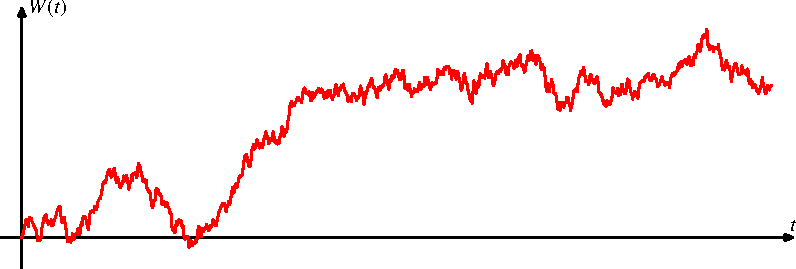
\includegraphics{chapters/images/stochastisch-1.pdf}
\caption{Wiener-Prozess $W(t)$ in Abh"angigkeit von der Zeit
\label{stochastisch:wiener}}
\end{figure}

\subsection{Konstruktion des Wiener-Prozesses}
Wir m"ussen eine Konstruktion angeben, mit der wir zu einem gegebenen
Interval $[0,T]$ eine Funktion $W(t)$ konstruieren k"onnen, die
die Eigenschaften des Wiener-Prozesses erf"ullt.

Zun"achst verlangen die Eigenschaften~1 und 2 des Wiener-Prozesses,
dass $X(T)$ eine normalverteilte Zufallsvariable ist mit Erwartungswert
$X(0)=0$ und Varianz $T$.
Da $X(t)$ ausserdem stetig sein soll, verwenden wir als erste Iteration
die lineare Funktion:
\[
W_1(t) = X(T)\frac{t}{T}
\]
Die Eigenschaft~3 verlangt, dass auch $X(T/2)$ normalverteilt ist mit
Erwartungswert $0$ und Varianz $T/2$.
Dies kann dadurch erreicht werden, dass wir $W_1$ durch einen 
Polygonzug $W_2$ ersetzen, der bei $t=T/2$ einen zus"atzlichen
Eckpunkt besitzt.
Wir bezeichnen den Unterschied zwischen $W_2$ und $W_1$ an der
Stelle $t=T/2$ mit
\[
Y=W_2(T/2)-W_1(T/2)=W_2(T/2) - W_1(T)/2.
\]
$Y$ muss so gew"ahlt werden, dass $W_2(T/2)$ eine normalverteilte
Zufallsvariable mit Erwartungswert $0$ und Varianz $T/2$ wird,
somit ist $Y$ auch normalverteilt.
Der Erwartungswert von $Y$ ist
\begin{align*}
E(Y)&=E(W_2(T/2) - W_1(T)/2)=E(W_2(T/2))-E(W_1(T))/2=0,
\end{align*}
es ist also nur noch die Varianz $\sigma^2_Y$ w"ahlbar.
Sie muss so gew"ahlt werden, dass $W_2(T/2)$ Varianz $T/2$
bekommt:
\begin{align*}
\operatorname{var}\biggl(W_2\biggl(\frac{T}2\biggr))\biggr))
&=
\operatorname{var}\biggl(W_1\biggl(\frac{T}2\biggr) + Y\biggr)
=
\frac{\operatorname{var}(W_1)}4 + \operatorname{var}Y
=
\frac{T}4 +\sigma_Y^2
\end{align*}
Es folgt $\sigma_Y^2=\frac{T}4$.

Wir m"ussen kontrollieren, ob die Inkremente unabh"angig sind.
Dazu berechnen wir der Erwartungswert des Produktes der
beiden Inkremente
\begin{align*}
W_2(T)-W_2\biggl(\frac{T}2\biggr)
&=
W_1(T)-\biggl(\frac{W_1(T)}2 + Y\biggr)
=
Y-\frac{W_1(T)}2
\\
W_2\biggl(\frac{T}2\biggr)-W_2(0)
&=
Y+
\frac{W_1(T)}2
\\
\biggl(W_2(T)-W_2\biggl(\frac{T}2\biggr)\biggr)
\biggl(W_2\biggl(\frac{T}2\biggr)-W_2(0)\biggr)
&=
\biggl(Y-\frac{W_1(T)}2\biggr)\biggl(Y+\frac{W_1(T)}2\biggr)
=
Y^2-\frac{W_1(T)^2}4
\\
E\biggl(
\biggl(W_2(T)-W_2\biggl(\frac{T}2\biggr)\biggr)
\biggl(W_2\biggl(\frac{T}2\biggr)-W_2(0)\biggr)
\biggr)
&=
E(Y^2)-E\biggl(\frac{W_1(T)^2}4\biggr)
=
\sigma_Y^2 - \frac14\operatorname{var}(W_1(T))
=
0
\end{align*}
Somit sind die Inkremente unabh"angig.

\begin{figure}
\centering
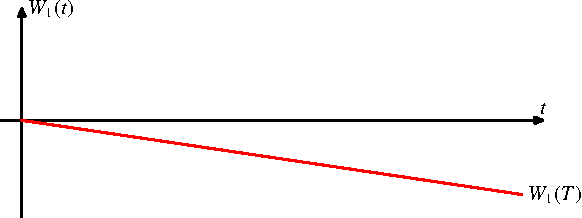
\includegraphics{chapters/images/stochastisch-3.pdf}\\
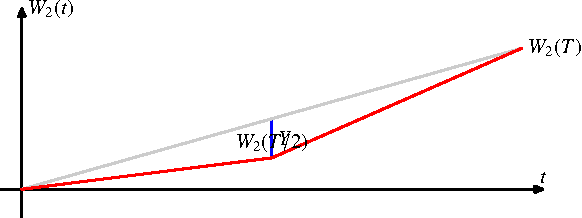
\includegraphics{chapters/images/stochastisch-4.pdf}\\
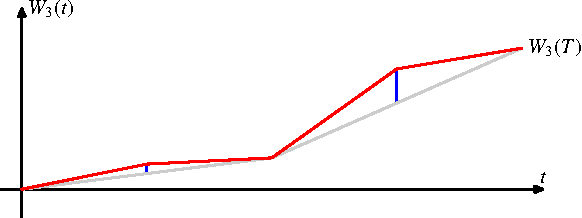
\includegraphics{chapters/images/stochastisch-5.pdf}\\
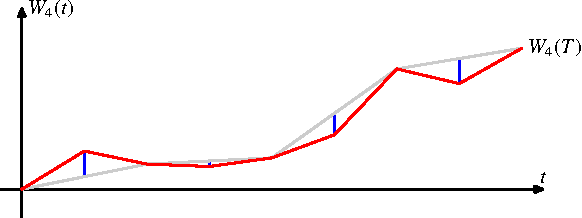
\includegraphics{chapters/images/stochastisch-6.pdf}\\
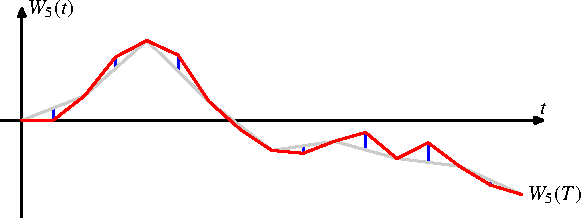
\includegraphics{chapters/images/stochastisch-7.pdf}
\caption{Schrittweise Konstruktion des Wiener-Prozesses als Grenzewert
der Folge $W_n(t)$, $n=1,\dots,5$
\label{stochastisch:folge1}}
\end{figure}
\begin{figure}
\centering
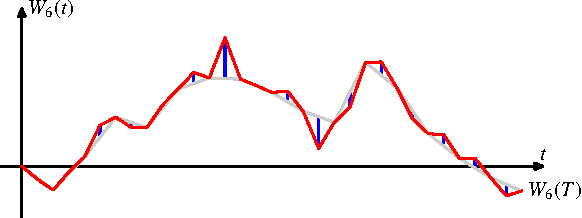
\includegraphics{chapters/images/stochastisch-8.pdf}\\
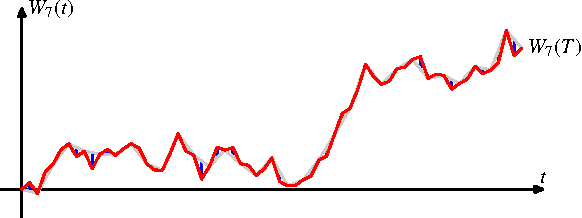
\includegraphics{chapters/images/stochastisch-9.pdf}\\
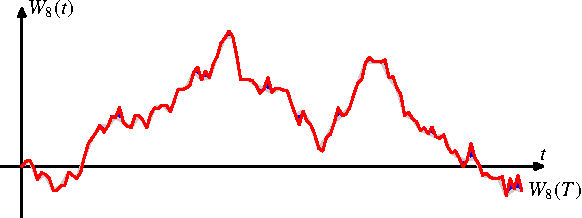
\includegraphics{chapters/images/stochastisch-10.pdf}\\
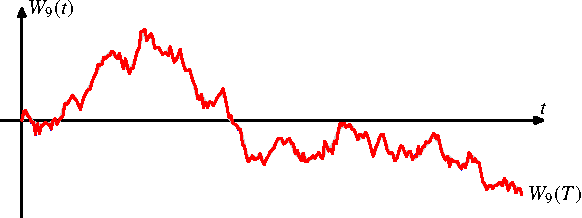
\includegraphics{chapters/images/stochastisch-11.pdf}\\
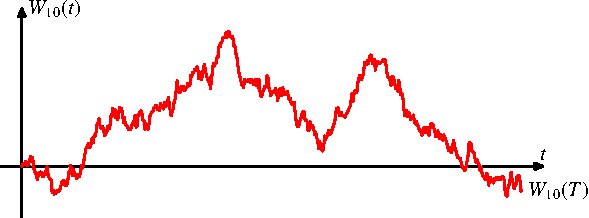
\includegraphics{chapters/images/stochastisch-12.pdf}
\caption{Schrittweise Konstruktion des Wiener-Prozesses als Grenzewert
der Folge $W_n(t)$, $n=6,\dots,10$
\label{stochastisch:folge2}}
\end{figure}

Diesen Prozess k"onnen wir fortsetzen: f"ur $W_3$ nehmen wir einen
Polygonzug mit zus"atzlichen Eckpunkten an den Stellen $T/4$ und $3T/4$.
Die Differenz zwischen $W_3$ und $W_2$ an diesen Stellen m"ussen
normalverteilt sein mit Erwartungswert $0$ und Varianz $T/8$.
Auf diese Weise k"onnen wir eine Folge $W_n$ von Prozessen konstruieren,
wie in den Abbildungen~\ref{stochastisch:folge1} und \ref{stochastisch:folge2}
dargestellt.

Dies reicht aber nicht.
F"ur eine vollst"andige Konstruktion muss man noch die folgenden zwei
Dinge zeigen.
\begin{compactenum}
\item
Der Grenzwert existiert tats"achlich.
Weil die einzelnen Zufallsvariablen $Y$ normalverteilt sind, k"onnen
sie beliebig grosse Werte annehmen.
Dies bedeutet auch, dass wir im Allgemeinen nicht davon ausgehen 
k"onnen, dass die Folge $W_n(t)$ konvergiert.
Zwar sind die Werte von $W_m$ an den Stellen $t_{k,n}=kT/2^{n-1}$ f"ur
$k=0,\dots,2^{n-1}$ fest, sobald $m\ge n$.
Zwischen diesen Werten k"onnen aber immer wieder grosse Werte auftreten,
so dass die Folge $W_n$ weder gleichm"assig noch punktweise konvergieren
kann.
Die Frage der Konvergenz muss daher als Konvergenz in einer Art Mittel 
angegangen werden.
\item
Die Forderung, dass die Inkremente $W(t)-W(s)$ und $W(s)-W(r)$ f"ur jedes 
Tripel $t \ge s\ge r$ unabh"angig sein m"ussen.
Die Konstruktion stellt nur sicher, dass dies gilt, wenn die Zeitpunkte
des Tripels Eckpunkte der Polygonkonstruktion sind.
\end{compactenum}

%
%
%
\section{Stochastische Differentialgleichungen\label{section:stochdgl}}
\rhead{Differentialgleichungen}
Wir m"ochten gerne eine Differentialgleichung f"ur den Zustand
$X(t)$ eines Systems l"osen, welches von Rauschen mit beeinfluss wird.
Eine solche Differentialgleichung k"onnten wir schreiben als
\[
\frac{dX(t)}{dt}
=
b(X(t)) + B(X(t))\frac{dW(t)}{dt}
\]
wobei $b$ die Rolle der Funktion $f$ aus
Abschnitt~\ref{section:anfangswertprobleme} spielt.
Die Ableitung von $W$ spielt die Rolle des Rauschens, wir wissen aber
bereits, dass $W$ nicht differenzierbar sein kann, die Gleichung
in dieser Form kann daher gar nicht sinnvoll sein.

Formal kann man die Gleichung mit $dt$ multiplizieren, so dass man
das formale Gleichungssystem
\begin{align*}
dX(t)
&=
b(X(t)) + B(X(t),t)\,dW(t)
\\
X(0)
&=
x_0
\end{align*}
erh"alt, aber auch in diesr Form sind die Ausdr"ucke $dX$ und $dW$ nicht
ohne zus"atzliche Definition sinnvoll.
Am ehesten hat man eine Chance, dieser Gleichung einen Sinn zu geben,
wenn man integriert:
\begin{align*}
X(t)=x_0+\int_0^t b(X(s))\,ds + \int_0^t B(X(s), s)\, dW,\qquad t>0.
\end{align*}
Das erste Integral ist ein gew"ohnliches Integral, denn wir
gehen davon aus, dass die Funktion $X(t)$ stetig ist.
Wenn $B=0$ ist, dann liefert diese Formel genau L"osungen der
urspr"unglichen Differentialgleichung.
Wir brauchen aber immer noch eine Interpretation des zweiten Integrals,
diese werden wir in Abschnitt~\ref{subsection:stochint} geben.

Nehmen wir f"ur den Moment an, dass die L"osung $X(t)$ gefunden werden
kann, und sei $u$ eine beliebig oft differenzierbare Funktion.
Wir erwarten, dass die Ableitung von $Y(t)=u(X(t))$ nach der
Kettenregel
\[
dY = u'\,dX = u'b\,dt + u'\,dW
\]
sein sollte.
Tats"achlich ist das Rauschen so stark, dass die Kr"ummung der Funktion
$u$ bereits eine Rolle spielt.
Bei einer gew"ohnlichen Differentialgleichung sind auf kleine Entfernungen
die zweiten Ableitungen von $u$ vernachl"assigbar.
Die schnellen, vom Rauschen verursachten Abweichungen f"uhren sind aber nicht
klein, so dass die korrekte Kettenregel bei Anwesenheit von Rauschen die
It\^o-sche Kettenregel wird, die stattdessen den Ausdruck
\[
dY =  \biggl(u'b + \frac12u''\biggr)\,dt + u'\,dW
\]
liefert.
Der Term $\frac12u''$ ist in der klassischen Analysis nicht vorhanden.
Wir m"ussen daher auch alle gewohnten Rechenregeln der Analysis "uberpr"ufen.

\subsection{Stochastische Integrale\label{subsection:stochint}}
\index{stochastisches Integral}
Wir m"ochten eine Definition f"ur ein Integral der Form
\[
\int_0^T G\,dW
\]
f"ur zwei stochastische Prozesse $G(t)$ und $W(t)$.

\subsubsection{Das Paley-Wiener-Zygmund Integral}
\index{Paley-Wiener-Zygmund Integral}
F"ur differenzierbare Funktionen $g(t)$ und $w(t)$ ist klar, was 
mit dem Integral gemeint ist:
\[
\int_0^T g(t)\,dw = \int_0^T g(t) w'(t)\,dt.
\]
Wenn $g(0)=g(T)=0$ ist, dann kann man dies mit Hilfe partieller Integration
vereinfachen:
\[
\int_0^T g(t)\,dw
=
\int_0^T g(t) w'(t)\,dt
=
[g(t)w(t)]_0^T
-
\int_0^T g'(t) w(t)\,dt
=
-\int_0^T g'(t) w(t)\,dt
\]
Diese letzte Formel ist aber auch geeignet als Definition des Integrals
f"ur eine brownsche Bewegung $W(t)$ an Stelle von $w(t)$.

\begin{definition}
F"ur eine stetig differenzierbare Funktion $g\colon[0,T]\to \mathbb R$ 
mit $g(0)=g(T)=0$, setze
\[
\int_0^T g\,dW = -\int_0^T g'(t) W(t)\,dt.
\]
\end{definition}

\begin{hilfssatz}
Erwartungswert und Varianz der Zufallsvariablen
\[
Z=\int_0^T g\,dW
\]
ist
\begin{compactenum}
\item $E(Z)=0$
\item $\operatorname{var}(Z)=\int_0^Tg(t)^2\,dt$
\end{compactenum}
\end{hilfssatz}

\begin{proof}[Beweis]
F"ur den Erwartungswert finden wir mit Hilfe der Rechenregeln f"ur den
Erwartungswert
\begin{align*}
E(Z)
&=
E\biggl(\int_0^T g\,dW\biggr)
=
E\biggl(
\int_0^T g'(t) W(t)\,dt
\biggr)
=
\int_0^T g'(t) \underbrace{E(W(t))}_{\textstyle =0}\,dt=0
\end{align*}
Die Varianz ist daher der Erwartungswert $E(Z^2)$, die wir ebenfalls unter
Verwendung der Rechenregeln berechnen k"onnen
\begin{align*}
E(Z^2)
&=
E\biggl(\biggl(\int_0^T g\,dW\biggr)^2\biggr)
=
E\biggl(
\biggl(
\int_0^T g'(t)W(t)\,dt
\biggr)^2
\biggr)
\\
&=
E\biggl(
\int_0^T g'(t)W(t)\,dt
\int_0^T g'(s)W(s)\,ds
\biggr)
=
E\biggl(
\int_0^T \int_0^T g'(t)W(t) g'(s)W(s) \,ds \,dt
\biggr)
\\
&=
\int_0^T\int_0^Tg'(t)g'(s) \underbrace{E(W(t)W(s))}_{\textstyle =t\wedge s}\,ds\,dt
\\
&=
\int_0^Tg'(t) \biggl(\int_0^t g'(s) s\,ds + \int_t^T g'(s)t\,ds\biggr)
\,dt
\\
&=
\int_0^T g'(t)\biggl(
\underbrace{[g(s)s]_0^t}_{\textstyle =tg(t)}-\int_0^t g(s)\,ds+t(\underbrace{g(T)}_{\textstyle =0}-g(t))
\biggr)\,dt
\\
&=
\int_0^T g'(t)\biggl(-\int_0^t g(s)\,ds\biggr)\,dt
\\
&=
\biggl[
g(t)\biggl(-\int_0^t\int_0^tg(s)\,ds\biggr)
\biggr]_0^T
+
\int_0^Tg(t)^2\,dt
\end{align*}
Damit ist die Behauptung bewiesen.
\end{proof}
Der Hilfssatz kann dazu verwendet werden, die Definition des Integrals auf
weitere Funktionen auszudehnen.
Eine Folge von Funktionen $g_n$ f"uhrt auf eine Folge von Werten des
Integrals. 
Um daraus eine Erweiterung des Integrals zu konstruieren, m"ussen wir 
definieren, was es heissen soll, dass die Folge $g_n$ konvergiert.
Wir verwenden die Norm
\[
\|f\|_2^2=\int_0^T f(t)^2 \,dt,
\]
um den Abstand zwischen Funktionen zu messen.
Eine Cauchy-Folge von Funktionen in dieser Norm ist dann eine Folge so,
dass f"ur jedes $\varepsilon>0$ ein $N>0$ existiert, so dass aus
$n,m>N$ folgt
\[
\|g_n-g_m\|_2^2=\int_0^T (g_n(t)-g_m(t))^2\,dt<\varepsilon.
\]
In diesem Fall gilt, dass
\[
E\biggl(
\biggl(
\int_0^T g_n\,dW
-
\int_0^T g_m\,dW
\biggr)^2
\biggr)
=
\int_0^T(g_m(t)-g_n(t))^2\,dt<\varepsilon
\]
Die Zufallsvariablen
\[
Z_n = \int_0^T g_n\,dW
\]
bildet daher eine Cauchy-Folge von quadratintegrierbaren Funktionen
in $L^2(\Omega)$, und wir k"onnen deren Grenzwert
\[
\int_0^T g\,dW
=
\lim_{n\to\infty}\int_0^T g_n\,dW
\]
als den verallgemeinerten Wert f"ur das Integral einer beliebigen Funktion
$g\in L^2([0,T])$ definieren.

\subsubsection{Riemann-Summen}
Die Verallgemeinerung des Paley-Wiener-Zygmund-Integral auf
quadratintegrierbare Funktionen ist allerdings nicht ausreichend, um
\[
\int_0^T W\,dW
\]
zu definieren.
Wir k"onnen aber noch weiter zur"uck gehen zur Definition des
Riemann-Integrals, und sie verallgemeinern auf einen stochastischen
Prozess.

\begin{definition}
Eine {\em Unterteilung} $P$ des Intevals $[0,T]$ ist eine endliche Menge
von Teilpunkten
\[
P=\{ 0=t_0<t_1<t_2<\dots<t_m=T\}.
\]
Die {\em Maschenweite} $|P|$ der Unterteilung $P$ ist
\[
|P|=\max_{0\le k\le m-1}|t_{k+1\mathstrut}-t_{k\mathstrut}|.
\]
F"ur ein festes $0\le \lambda\le 1$ setzen wir
\[
\tau_k = (1-\lambda)t_{k\mathstrut}+\lambda t_{k+1\mathstrut}.
\]
\end{definition}
F"ur $\lambda=0$ ist $\tau_k=t_k$, f"ur $\lambda=1$ gilt $\tau_k=t_{k+1}$.
F"ur andere Werte von $\lambda$ ist $\tau_k$ ein Punkt im Inneren des
Intervals $[t_k,t_{k+1}]$.
Wie "ublich kann eine solche Unterteilung dazu verwendet werden, die 
Riemann-Summe als Approximation des Integrals zu definieren:

\begin{definition}
Die Riemann-Summe von f"ur $\int W\,dW$ und die Unterteilung $P$ ist
\[
R=R(P,\lambda) = \sum_{k=0}^{m-1} W(\tau_k)(W(t_{k+1})-W(t_k)).
\]
\index{Riemann-Summe}
\end{definition}

\begin{hilfssatz}
\label{stochastisch:quadrvariation}
Sei
\[
P^{(n)}
=
\{0=t_0^{(n)}<t_1^{(n)}<\dots < t_{m_n}^{(n)}=T\}
\]
eine Folge von Unterteilungen des Intervals $[0,T]$ derart,
dass die Maschenweite gegen $0$ strebt, dann gilt
\[
\lim_{n\to\infty}
\sum_{k=0}^{m_n-1} \bigl(W(t_{k+1}^{(n)})-W(t_{k}^{(n)})\bigr)^2
=T
\]
in $L^2(\Omega)$.
\end{hilfssatz}

\begin{proof}[Beweis]
Konvergenz in $L^2(\Omega)$ bedeutet, dass der Erwartungswert der
quadratische Abweichung gegen $0$ streibt.
Setzen wir
\[
Q_n
= 
\sum_{k=0}^{m_n-1} \left(W(t_{k+1}^{(n)})-W(t_{k}^{(n)})\right)^2,
\]
und m"ussen untersuchen, ob $E((Q_n - T)^2)$ gegen $0$ strebt.
Wir beginnen mit der Bemerkung, dass
\begin{align*}
Q_n-T
&=
\sum_{k=0}^{m_n-1}
\left((W(t_{k+1}^{(n)})-W(t_{k}^{(n)}))^2 - (t_{k+1}^{(n)}-t_k^{(n)})\right).
\end{align*}
Die einzelnen Differenzen k"urzen wir ab als
\begin{align*}
Y_k
&=
\frac{W(t_{k+1}^{(n)})-W(t_k^{(n)})}{\sqrt{t_{k+1}^{(n)}-t_{k}^{(n)}}},
\\
\Delta_k
&=
t_{k+1}^{(n)}-t_k^{(n)}.
\end{align*}
F"ur $j\ne k$ sind $Y_j^{(n)}$ und $Y_{k}^{(n)}$ unabh"angig.
Ausserdem ist $Y_k$ standardnormalverteilt, also $E(Y_k)=0$
und $E(Y_k^2)=1$.
Die Summanden in der Summe lassen sich damit kompakter ausdr"ucken:
\begin{align*}
Q_n-T
&=
\sum_{k=0}^{m_n-1} (Y_k^2-1) \Delta_k
\end{align*}
Dies k"onnen wir in $E((Q_n-T)^2)$ einsetzen:
\begin{align*}
E((Q_n-T)^2)
&=
\sum_{k=0}^{m_n-1}
\sum_{j=0}^{m_n-1}
E\biggl(
(Y_k^2-1)\Delta_k
(Y_j^2-1)\Delta_j
\biggr)
\end{align*}
Die Doppelsumme kann zerlegt werden in Terme mit $j=k$ und $j\ne k$.

In den Terme mit $j\ne k$ sind die $Y_k$ und $Y_j$ voneinander unabh"angig,
der Erwartungswert des Produktes kann daher in das Produkt der Erwartungswerte
zerlegt werden:
\begin{align*}
E\left(
(Y_k^2-1)\Delta_k
(Y_j^2-1)\Delta_j
\right)
&=
E(Y_k^2-1)
E(Y_j^2-1)
\Delta_k
\Delta_j
\\
&=
\bigl(E(Y_k^2) -1\bigr)
\bigl(E(Y_j^2) -1\bigr)
\Delta_k
\Delta_j
=0
\end{align*}
Im letzten Schritt haben wir verwendet, dass $E(Y_k^2)=\operatorname{var}Y_k=1$
ist.

Die Terme mit $j=k$ sind 
\begin{align*}
E((Q_n-T)^2)
&=
\sum_{k=0}^{m_n-1} E\biggl((Y_k^2-1)^2\Delta_k^2\biggr)
\\
&=
\sum_{k=0}^{m_n-1} E\bigl((Y_k^2-1)^2\bigr)\Delta_k^2
\le 
\biggl(\sum_{k=0}^{m_n-1} E\bigl((Y_k^2-1)^2\bigr)\Delta_k\biggr)\, |P^{(n)}|
\end{align*}
Im letzten Schritt haben wir einen Faktor $\Delta_k$ aus der Summe
herausgenommen und durch die Maschenweite $|P^{(n)}|$ abgesch"atzt.

Da $Y_k$ standardnormalverteilt ist, ist der Erwartungswert $E((Y_k^2-1)^2)$
unabh"angig von $k$, wir nennen diesen Wert $C$, der genaue Wert ist
nicht wichtig\footnote{Man kann den Wert nat"urlich wie folgt berechnen:
\begin{align*}
E((Y_k^2-1)^2)
&=
E(Y_k^4-2Y_k^2+1)
=
E(Y_k^4)-2E(Y_k^2)+E(1)
=
6-2+1=5.
\end{align*}}.
Damit l"asst sich die Differenz jetzt unabh"angig von $k$ absch"atzen
\begin{align*}
E((Q_n-T)^2)
&
\le
C\biggl(\sum_{k=1}^{m_n}\Delta_k\biggr)\, |P^{(n)}|
=CT|P^{(n)}|.
\end{align*}
Da die Maschenweite $|P^{(n)}|\to 0$ f"ur $n\to\infty$ folgt, dass
$Q_n\to T$ in $L^2(\Omega)$.
\end{proof}

\begin{hilfssatz}
\label{stochastisch:intwdw}
Sei $P^{(n)}$ eine Folge von Unterteilungen des
Intervals $[0,T]$ derart, dass die Maschenweite gegen $0$ strebt und
sei $R_n=R(P^{(n)},\lambda)$ die zugeh"orige Riemann-Summe.
Dann gilt
\[
\lim_{n\to\infty} R_n = \frac{W(T)^2}2 + \biggl(\lambda-\frac12\biggr)T
\]
als Funktion in $L^2(\Omega)$.
\end{hilfssatz}

\begin{proof}[Beweis]
Wir m"ussen die Riemann-Summe
\begin{align*}
R_n
&=
\sum_{k=0}^{m_n-1}
W(\tau_k) (W(t_{k+1}^{(n)})-W(t_k^{(n)}))
\end{align*}
durch Inkremente von Werten von $W(t)$ ausdr"ucken, konkret durch
\[
W(t_{k+1}^{(n)})-W(t_k^{(n)}),\quad
W(t_{k+1}^{(n)})-W(\tau_k^{(n)})
\quad \text{und} \quad
W(\tau_k^{(n)})-W(t_k^{(n)}).
\]
Um herauszufinden, wie dies m"oglich sein k"onnte, k"urzen wir die Werte
von $W$ ab durch
\[
a_k=W(t_k^{(n)}),\quad
b_k=W(\tau_k^{(n)})\quad\text{und}\quad
c_k=W(t_{k+1}^{(n)}),
\]
wobei wir im folgenden zur Vereinfachung der Rechnung die Indizes auch
weglassen.
Jetzt versuchen wir $b(c-a)$ durch andere Differenzen auszudr"ucken.
\begin{align*}
(b-a)^2
&=
b^2-2ab + a^2
\\
(c-a)^2
&=
c^2-2ac+a^2
\\
(c-b)(b-a)
&=
cb-b^2-ac+ab
\end{align*}
Um den Ausdruck $b(c-a)$ zu produzieren, muss der letzte Term verwendet
werden, denn er ist der einzige, der $bc$ enth"alt.
Dann muss aber auch der erste Term verwendet werden, um den Term $b^2$ zum
Verschwinden  zu bringen.
Ebenso muss der zweite Term $\frac12$-mal subtrahiert werden, damit der
Ausdruck $ac$ wegf"allt:
\begin{align*}
(b-a)^2-\frac12(c-a)^2+(c-b)(b-a)
&=
(b^2-2ab + a^2)
-\frac12(c^2-2ac+a^2)
+(cb-b^2-ac+ab)
\\
&=
cb-ab + \frac12a^2
-\frac12c^2
\end{align*}
Die quadratischen Terme sind $\frac12c_k^2=\frac12W(t_{k+1}^{(n)})^2$ und
$\frac12a_k^2=\frac12W(t_{k}^{(n)})^2$, die sich in aufeinanderfolgenden Termen
jeweils wegheben.
Nur der erste und letzte Term bleibt in der Summe bestehen, was wir
aber leicht korrigieren k"onnen.
So finden wir daher:
\begin{align*}
R_n
&=
\underbrace{
\sum_{k=0}^{m_n-1} (b_k-a_k)^2
}_{\textstyle\to\lambda T}
-
\underbrace{
\frac12\sum_{k=0}^{m_n-1} (c_k-a_k)^2
}_{\textstyle\to T}
+\sum_{k=0}^{m_n-1} (c_k-b_k)(b_k-a_k)
- \frac12a_0^2
+ \frac12c_{m_n-1}^2
\end{align*}
Die zweite Summe wurde im Hilfssatz~\ref{stochastisch:quadrvariation}
berechnet, dort wurde gefunden, dass die Summe f"ur $n\to\infty$ gegen $T$
konvergiert.
Mit der gleichen Rechnung wie in \ref{stochastisch:quadrvariation}
kann man finden, dass die erste Summe gegen $\lambda T$ strebt.

Die Inkremente in der dritten Summe sind unabh"angig voneinander, daher
verschwinden die Erwartunsgewerte gemischter Produkte, es bleiben nur
die Terme
\begin{align*}
E\biggl(\biggl(\sum_{k=0}^{m_n-1}(c_k-b_k)(b_k-a_k)\biggr)^2\biggr)
&=
\sum_{k=0}^{m_n-1}
E\bigl((c_k-b_k)^2\bigr)E\bigl((b_k-a_k)^2\bigr)
\\
&=
\sum_{k=0}^{m_n-1}
E\bigl((W(t_{k+1}^{(n)})-W(\tau_k^{(n)}))^2\bigr)E\bigl((W(\tau_k^{(n)})-W(t_k^{(n)})^2\bigr)
\\
&=
\sum_{k=0}^{m_n-1}
(t_{k+1}^{(n)}-\tau_k^{(n)}) (\tau_k^{(n)}-t_k^{(n)})
\\
&=
\sum_{k=0}^{m_n-1}
(1-\lambda)(t_{k+1}^{(n)}-t_k^{(n)}) \lambda(t_{k+1}^{(n)}-t_k^{(n)})
\\
&\le 
(1-\lambda)\lambda
|P^{(n)}|
\sum_{k=0}^{m_n-1}
(t_{k+1}^{(n)}-t_k^{(n)})
\le (1-\lambda)\lambda T|P^{(n})|\to 0
\end{align*}
f"ur $n\to\infty$.
Damit ist gezeigt, dass die Riemann-Summe in $L^2(\Omega)$ gegen
\[
R_n\to
\frac{W(T)^2}2+\biggl(\lambda-\frac12\biggr)T
\]
konvergiert.
\end{proof}

\subsubsection{Das It\^o-Integral}
Ausgehend von der Riemann-Summe und den f"ur sie hergeleiteten Eigenschaften
wollen wir jetzt ein Integral
\[
\int_0^T G\,dW
\]
f"ur eine breitere Klasse von stochastischen Prozessen $G$ definieren.
Der erste Schritt dazu, ist das Integral f"ur Stufenprozesse zu definieren.

\begin{definition}
\index{Stufenprozess}
Ein stochastischer Prozess $G(t)$ ist eine {\em Stufenprozess}, wenn es eine
Unterteilung $P=\{0=t_0<t_1<\dots<t_m=T\}$ gibt derart, dass
$G(t)=G(t_k)$ f"ur $t_k\le t<t_{k+1}$.
\end{definition}

\begin{definition}
Ist $G$ ein Stufenprozess, dann ist das {\em It\^o-Integral} von $G$ definiert
als
\[
\int_0^TG\,dW = \sum_{k=0}^{m-1}G(t_k)(W(t_{k+1})-W(t_k)).
\]
Das It\^o-Integral ist eine Zufallsvariable.
\end{definition}

Das It\^o-Integral hat die folgenden Eigenschaften
\begin{hilfssatz}
Wenn $G$ und $H$ Stufenprozesse sind und $a,b\in\mathbb R$, dann gilt
\begin{compactenum}
\item Das It\^o-Integral ist linear:
\[
\int_0^T aG+bH\,dW
=
a\int_0^T G\,dW + b \int_0^TH\,dW
\]
\item Der Erwartungswert des It\^o-Integrals ist $0$:
\[
E\biggl(\int_0^T G\,dW\biggr)=0.
\]
\item Die Varianz des It\^o-Integrals ist
\[
E\biggl(\biggl(\int_0^T G\,dW\biggr)^2\biggr)
=
E\biggl(\int_0^T G^2\,dt\biggr)
\]
\end{compactenum}
\end{hilfssatz}

\begin{proof}[Beweis]
F"ur die Linearit"at verwenden wir eine Unterteilung $P$, f"ur die sowohl
$G$ also auch $H$ ein ein Stufenprozess ist.
Dann gilt
\begin{align*}
\int_0^T aG+bH\,dW
&=
\sum_{k=0}^{m-1} (aG(t_k)+bH(t_k))(W(t_{k+1})-W(t_k))
\\
&=
a\sum_{k=0}^{m-1} G(t_k)(W(t_{k+1})-W(t_k))
+
b\sum_{k=0}^{m-1} H(t_k)(W(t_{k+1})-W(t_k))
\\
&=a\int_0^TG\,dW+b\int_0^TH\,dW
\end{align*}
womit die Linearit"at bewiesen ist.

F"ur den Erwartungswert berechnen wir mit Hilfe einer passenden Unterteilung
\begin{align*}
E\biggl(\int_0^T G\,dW\biggr)
&=
E\biggl(\sum_{k=0}^{m-1} G(t_k) (W(t_{k+1}) - W(t_k))\biggr)
\\
&=
\sum_{k=0}^{m-1} E(G(t_k)) \underbrace{E(W(t_{k+1}) - W(t_k))}_{\textstyle =0}=0.
\end{align*}
Damit ist 2.~beweisen.

F"ur die Berechnung der Varianz verwendet wieder die Unabh"angigkeit der
Inkremente:
\begin{align*}
E\biggl(\biggl(\int_0^T G\,dW\biggr)^2\biggr)
&=
E\biggl(\biggl(\sum_{k=0}^{m-1}G(t_k)(W(t_{k+1})-W(t_k))\biggr)^2\biggr)
\\
&=
E\biggl(
\sum_{k=0}^{m-1}G(t_k)(W(t_{k+1})-W(t_k))
\sum_{j=0}^{m-1}G(t_j)(W(t_{j+1})-W(t_j))
\biggr)
\\
&=
\sum_{k=0}^{m-1}
\sum_{j=0}^{m-1}
E(G(t_k) G(t_j)
(W(t_{k+1})-W(t_k))
(W(t_{j+1})-W(t_j))
)
\\
&=
\sum_{k=0}^{m-1}
E(G(t_k)^2) E(W(t_{k+1})-W(t_k))^2)
\\
&=
\sum_{k=0}^{m-1}
E(G(t_k)^2) (t_{k+1}-t_k)
=
E\biggl(
\sum_{k=0}^{m-1}
G(t_k)^2 (t_{k+1}-t_k)
\biggr)
=E\biggl(\int_0^T G(t)^2\,dt\biggr).
\end{align*}
Somit ist auch 3.~bewiesen.
\end{proof}

Die Bedeutung der dritten Eigenschaft besteht darin, dass eine
Folge von Stufen-Prozessen, die $L^2(0,T)$ konvergiert, zu einer
konvergenten Folge von It\^o-Integralen f"uhrt.

\begin{definition}
\index{It\^o-Integral}
Ist $G$ ein beliebiger auf $[0,T]$ quadratintegrierbarer Prozess,
und $G_n$ eine Folge von stochastischen Prozessen, die in $L^2([0,T])$
gegen $G$ konvergiert.
Dann ist des It\^o-Integral von $G$
\[
\int_0^T G\,dW
=
\
\lim_{n\to\infty} \int_0^T G_n\,dW
\]
\end{definition}

\begin{beispiel}
Wir haben die Riemann-Summe f"ur $G=W$ bereits in
Hilfssatz~\ref{stochastisch:intwdw} berechnet, daher k"onnen wir jetzt
das It\^o-Integral angeben:
\[
\int_0^t W\,dW
=
\frac12 W(t)^2 -\frac{t}2.
\]
In differentieller Form:
\[
d(W^2)
=
2W\,dW + t.
\]
Dies ist ein Spezialfall der sp"ater zu untersuchenden It\^o-Produktregel.
\end{beispiel}

Das It\^o-Integral hat die folgenden Eigenschaften:

\begin{satz}
\label{satz:ito-integral}
Seien $G$ und $H$ auf $[0,T]$ quadratintegrierbare stochastische Prozesse
und $a,b\in\mathbb R$. Dann gilt
\begin{compactenum}
\item Das It\^o-Integral ist linear:
\[
\int_0^T aG+bH\,dW
=
a\int_0^TG\,dW
+
b\int_0^TH\,dW
\]
\item Der Erwartungswert des It\^o-Integrals ist
\[
E\biggl(\int_0^T G\,dW\biggr)=0
\]
\item Die Varianz des It\^o-Integrals ist
\[
E\biggl(\biggl(\int_0^TG\,dW\biggr)^2\biggr)
=
E\biggl(\int_0^T G^2\,dt\biggr).
\]
\end{compactenum}
\end{satz}

Mit dem It\^o-Integral k"onnen wir jetzt alle Komponenten einer
stochastischen Differentialgleichung definieren.
Zun"achst k"onnen wir f"ur jeden auf $[0,T]$ quadratintegrierbaren Prozess $G$ 
und f"ur jede integrierbare Funktion $F\in L^1([0,T])$ die Gr"ossen
\begin{align*}
\int_s^r F(t)\,dt&=\int_0^r F(t)\,dt - \int_0^s F(t)\,dt
\\
\int_s^r G\,dW&=\int_0^r G\,dW - \int_0^s G\,dW
\end{align*}
definieren.
\begin{definition}
Wenn $X$ ein stochastischer Prozess ist, der
\[
X(r)=X(s)+\int_s^rF(t)\,dt + \int_s^tG\,dW
\]
erf"ullt, dann sagt man $X$ habe das {\em stochastische Differential}
\[
dX=F\,dt + G\,dW.
\]
\end{definition}

%
%
%
\subsection{Rechenregeln}
Bisher wissen wir nur, dass das It\^o-Integral linear ist, dies reicht
aber nicht f"ur einen Kalk"ul, mit dem wir hoffen k"onnen,
Differentialgleichungen zu l"osen.u
Dazu brauchen wir mindestens noch eine Kettenregel und eine
Produktregel.

\begin{satz}[It\^o's Kettenregel]
\index{It\^o-Kettenregel}
Falls $X$ das stochastische Differential
\[
dX=F\,dt + G\,dW
\]
hat, und falls $u\colon \mathbb R\times [0,T]\to\mathbb R$ eine
stetig differenzierbare Funktion.
Dann hat die Funktion $Y(t)=u(X(t), t)$ das stochastische Differential
\begin{align*}
du(X,t)
&=\frac{\partial u}{\partial t}\,dt + \frac{\partial u}{\partial x}\,dX 
+\frac12\frac{\partial u^2}{\partial x^2}G^2\,dt
\\
&=
\biggl(
\frac{\partial u}{\partial t}+\frac{\partial u}{\partial x}F
+\frac12\frac{\partial^2u}{\partial x^2}G^2
\biggr)\,dt
+
\frac{\partial u}{\partial x}G\,dW.
\end{align*}
\end{satz}
Bis auf den Term in den zweiten Ableitungen sind die Terme genau
diejenigen, die man von der klassischen Kettenregel her erwarten
k"onnte.

\begin{beispiel}
Potenzen eines Wiener-Prozesses.
Sei $u(x)=x^m$ und $X=W$, $F=0$ und $G=1$.
Also ist $Y=W^m$.
Dann hat nach der It\^o-schen Kettenregel das stochastische Differential
\[
d(W^m)
=
\frac12m(m-1)W^{m-2}\,dt + mW^{m-1}\,dW.
\]
Im Spezialfall $m=2$ folgt
\[
dW^2 = 2W\,dW + dt.
\]
Dies haben wir schon als Resultat von
Hilfssatz~\ref{stochastisch:intwdw} gefunden.
\end{beispiel}

\begin{beispiel} Wir betrachten die Funktion
$u(x,t)=e^{\lambda x-\frac12\lambda^2 t}$, und wie vorhin $X=W$, $F=0$
und $G=1$.
Es folgt
\begin{align*}
d\biggl(
e^{\lambda W(t)-\frac12\lambda^2 t}
\biggr)
&=
\biggl(
-\frac12\lambda^2 e^{\lambda W-\frac12\lambda^2 t}
+
\frac12\lambda^2 e^{\lambda W-\frac12\lambda^2 t}
\biggr)\,dt
+
\lambda e^{\lambda W -\frac12\lambda^2 t}\,dW
\\
dY&=\lambda Y\,dW
\end{align*}
also ist der Prozess $Y$ eine L"osung der stochastischen Differentialgleichung
\begin{align*}
dY&=\lambda Y\,dW
\\
Y(0)&=1.
\end{align*}
Dieses Beispiel zeigt, dass der entwickelte Kalk"ul dazu geeignet sein kann,
stochastische Differentialgleichungen zu l"osen.
\end{beispiel}

\begin{satz}[Produktregel von It\^o]
\index{It\^o-Produktregel}
\index{Produktregel von It\^o}
Falls die Prozesse $X_1$ und $X_2$ die stochastischen Differentiale
\begin{align*}
dX_1
&=
F_1\,dt + G_1\,dW
\\
dX_2
&=
F_2\,dt + G_2\,dW
\end{align*}
haben, dann ist
\begin{equation}
d(X_1X_2)
=
X_2\,dX_1 + X_1\,dX_2 + G_1G_2\,dt,
\label{stochastisch:ito-produkt}
\end{equation}
dies ist die {\em It\^o-sche Produktformel}.
\end{satz}

F"ur den Beweis der Kettenregel brauchen wir die Produktregel, wir geben
daher zuerst einen Beweis f"ur die Produktregel an.

\begin{proof}[Beweis der Produktformel]
Die integrierte Form der Produktregel besagt, dass 
\begin{equation}
X_1(r)X_2(r)-X_1(0)X_2(0)
=
\int_0^r X_2\,dX_1 + \int_0^r X_1\,dX_2 + \int_0^r G_1G_2\,dt
\label{stochastisch:ito-produkt-integriert}
\end{equation}
diese m"ussen wir nachrechnen.
Wir nehmen an der Einfachheit halber an, dass $X_1(0)=X_2(0)=0$ ist.

1.~Wir nehmen zus"atzlich an, dass die Funktion $G_i$ und $F_i$ nicht von
der Zeit abh"angen.
Dies bedeutet, dass sich die stochastische Differentialgleichung
$dX_i=F_i\,dt+G_i\,dW$ integrieren l"asst:
\[
X_i(t) = \int_0^t F_i\,d\tau + G_i\int_0^r dW =  F_it+G_iW(t).
\]
Diese Bedingung werden wir im zweiten Schritt wieder aufheben.
Wir berechnen die rechte Seite der integrierten
Produktregel~(\ref{stochastisch:ito-produkt-integriert}):
\begin{align*}
\int_0^r X_2\,dX_1 + X_1\,dX_2 + G_1G_2\,dt
&=
\int_0^rX_1F_2+X_2F_1\,dt + \int_0^r X_1G_2+X_2G_1\,dW + \int_0^r G_1G_2\,dt
\\
&=
\int_0^r(F_1t+G_1W)F_2+(F_2t+G_2W)F_1\,dt
\\
&\qquad
+ \int_0^r (F_1t+G_1W)G_2+(F_2t+G_2W)G_1\,dW + \int_0^r G_1G_2\,dt
\\
&=F_1F_2r^2+(G_1F_2+G_2F_1)\underbrace{\biggl(\int_0^rW\,dt + \int_0^rt\,dW\biggr)}_{\textstyle = rW(r)}
\\
&\qquad
+G_1G_2\cdot \underbrace{2\int_0^r W\,dW}_{\textstyle W(r)^2-r}
+ G_1G_2\underbrace{\int_0^r\,dt}_{\textstyle =r}
\\
&= 
F_1F_2r^2 + (G_1F_2+G_2F_1)rW(r) + G_1G_2W(r)^2
\\
&= 
F_1r\cdot F_2r + F_2r\cdot G_1W(r)+F_1r\cdot G_2W(r) + G_1W(r)\cdot G_2W(r)
\\
&= 
(F_1r + G_1W(r))\cdot(F_2r +  G_2W(r))
=
X_1(r) \cdot X_2(r).
\end{align*}
Dies ist die linke Seite von (\ref{stochastisch:ito-produkt-integriert}), die
damit f"ur diesen Spezialfall bewiesen ist.

2.~Wir ersetzen jetzt die Konstanten $G_i$ und $F_i$ durch Stufenprozesse.
Es gibt eine Unterteilung des Intervals $[0,T]$ so, dass die Prozesse $G_i$
und $F_i$ in jedem Teilinterval konstant sind.
In jedem solchen Teilinterval gilt daher die Ito-Produktformel, und damit
auch f"ur das ganze Interval.

3.~Im allgemeinen Fall k"onnen wir die Prozesse $G_i$ und $F_i$ mit Hilfe
einer Formel von Stufenprozessen $G_i^n$ und $F_i^n$ approximieren.
Wir k"onnen zus"atzlich fordern, dass
\[
E\biggl(\int_0^T |F_i^n-F_i|\,dt\biggr)\to 0
\qquad\text{und}\qquad
E\biggl(\int_0^T (G_i^n-G_i)^2\,dt\biggr)\to 0,
\]
was wir weiter unten brauchen.
Es gibt nach dem zweiten Schritt eine Folge von Prozessen $X_i^n$ mit
\[
X_i^n(t) = X_i(0) + \int_0^t F_i^n\,d\tau + \int_0^t G_i^n\,dW,
\]
f"ur die jeweils die Produktregel gilt.
\begin{align*}
X_i^n(r)X_i^n(r)-X_i^n(s)X_i^n(s)
&=
\int_0^r X_2^n\,dX_1^n+\int_0^r X_1^n\,dX_2^n + \int_0^r G_1^nG_2^n\,dW
\\
&=
\int_0^r X_2^nF_1^n\,dt
+
\int_0^r X_2^nG_1^n\,dW
+
\int_0^r X_1^nF_2^n\,dt
+
\int_0^r X_1^nG_2^n\,dW
+
\int_0^r G_1^nG_2^n\,dW
\\
\intertext{Der Grenz"ubergang $n\to\infty$ f"uhrt auf}
X_i(r)X_i(r)-X_i(s)X_i(s)
&=
\int_0^r X_2F_1\,dt
+
\int_0^r X_2G_1\,dW
+
\int_0^r X_1F_2\,dt
+
\int_0^r X_1G_2\,dW
+
\int_0^r G_1G_2\,dW
\end{align*}
Damit ist die Produktformel bewiesen.
\end{proof}

\begin{proof}[Beweis der Kettenregel]
Der Beweis der Kettenregel verwendet, dass die Funktion $u(x,t)$ durch
Polynome approximiert werden kann.
Wir m"ussen also zun"achst die Kettenregel f"ur Polynome in $x$ beweisen,
und dann mit Hilfe eines Grenz"ubergangs mit approximierenden Polynomen
den allgemeinen Fall gewinnen.

1. Sei $u(x)=x^m$, wir behaupten, dass
\[
d(X^m)=mX^{m-1}\,dX + \frac12m(m-1)X^{m-2}G^2\,dt,
\]
dies ist die It\^o-Produktformel f"ur $u(x)=x^m$.
Wir beweisen diese Formel durch vollst"andige Induktion.
F"ur $m=0$ ist sie trivialerweise korrekt.
Wir nehmen daher an, dass Sie f"ur $m-1$ gilt, dass also
\begin{align*}
d(X^{m-1})
&=
(m-1)X^{m-2}\,dX + \frac12(m-1)(m-2)X^{m-3}G^2\,dt
\\
&=
(m-1)X^{m-2}F\,dt + (m-1)X^{m-2}G\,dW + \frac12(m-1)(m-2)X^{m-3}G^2\,dt.
\end{align*}
Dies wenden jetzt die Produktregel auf $X^m = XX^{m-1}$ an.
F"ur $X_1=X$ ist $G_1=G$, und $X_2=X^{m-1}$ und
\[
G_2
=
(m-1)X^{m-2}G
\]
\begin{align*}
d(X^m)
&=
d(XX^{m-1})
=
X\,d(X^{m-1}) + X^{m-1}\,dX +G_1G_2\,dt
\\
&=
X\biggl( (m-1)X^{m-2}\,dX + \frac12(m-1)(m-2)X^{m-3}G^2\,dt\biggr)
+
X^{m-1}\,dX
+
(m-1)X^{m-2}G^2\,dt
\\
&=
mX^{m-1}\,dX
+\biggl(\frac12(m-2)+1\biggr)(m-1)X^{m-2}G^2\,dt
\\
&=
mX^{m-1}\,dX +\frac12m(m-1)X^{m-2}G^2\,dt,
\end{align*}
damit ist der Induktionsschritt vollzogen.

Wegen der Linearit"at der Ableitung ist die Kettenregel damit
f"ur beliebige Polynome in $x$ bewiesen.

2.~Wir approximieren die Funktion $u(x,t)$ jetzt als Produkt
$u(x,t)=f(x)g(t)$, wobei $f(x)$ und $g(t)$ Polynome sein sollen.
Dann gilt
\begin{align*}
d(u(X,t))
&=
d(f(X)g)
=
f(X)\,dg + g\,df(X)
\\
&=
f(X)g'\,dt + g\biggl(f'(X)\,dX + \frac12 f''(X)G^2\,dt\biggr)
\\
&=
\frac{\partial u}{\partial t}\,dt
+
\frac{\partial u}{\partial x}\,dX
+
\frac12\frac{\partial^2u}{\partial x^2}G^2\,dt.
\end{align*}
Die It\^o-Kettenregel ist damit gezeigt f"ur ein Produkt von Polynomen.

3.~Sei jetzt $u^n$ eine Folge von Polynomen wie im zweiten Schritt,
so dass $u^n$ sowie die Ableitungen gegen $u$ gleichm"assig konvergieren:
\[
u^n\to u,
\qquad
\frac{\partial u^n}{\partial t} \to \frac{\partial u}{\partial t},
\qquad
\frac{\partial u^n}{\partial x} \to \frac{\partial u}{\partial x},
\qquad
\frac{\partial^2 u^n}{\partial x^2} \to \frac{\partial^2 u}{\partial x^2}.
\]
F"ur jedes $u^n$ gilt die It\^o-Kettenregel:
\[
u^n(X(r),r)-u^n(X(0),0)
=
\int_0^r
\frac{\partial u^n}{\partial t}
+
\frac{\partial u^n}{\partial x}F
+
\frac12 \frac{\partial^2 u^n}{\partial x^2}G^2\,dt
+
\int_0^r\frac{\partial u^n}{\partial x}G\,dW,
\]
durch Grenz"ubergang $n\to \infty$ erhalten wir daraus die allgemeine
Form der It\^o-Kettenregel.
\end{proof}

%
% Beispiele 
%
\subsection{L"osungen von stochastischen Differentialgleichungen}
In diesem Abschnitt betrachten wir einige Beispiele von stochatischen
Differentialgleichungen und verwenden die im vorangegangenen Abschnitt
diskutierten Rechenregeln verwendet werden k"onnen, die L"osungen
zu finden.

\subsubsection{Lineare stochastische Differentialgleichung mit $F=0$}
Sei $g$ eine stetige Funktionen, man finde eine L"osung der
Differenzialgleichung
\begin{equation}
\begin{aligned}
dY&=gY\,dW\\
Y(0)&=1.
\end{aligned}
\label{stochastisch:beispiel1-dgl}
\end{equation}
Man beachte, dass ohne den stochastischen Einfluss nur noch die Gleichung
$dY=0$ "ubrig bleibt, in diesem Fall ist also $Y$ einfach nur eine
Konstante, $Y(t)=1$.
Wir k"onnen aber auch nicht erwarten, dass der Erwartungswert der
L"osung durch die L"osung $Y(t)=1$ gegeben ist.
Die Gleichung ist zwar linear, aber die Wirkung der stochastischen
Schwankungen ist proportional zum aktuellen Wert von $Y$.

W"are $W$ einfach nur eine differenzierbare Funktion, dann w"urde die
Differentialgleichung~(\ref{stochastisch:beispiel1-dgl}) zu der
gew"ohnlichen Differentialgleichung
\begin{align*}
\frac{\dot Y}{Y} &= g\dot W,
\\
\intertext{die durch direkte Integration gel"ost werden kann:}
\frac{d}{dt}\log Y&= g(t) \dot W(t)
\\
\log Y(t)&=\int_0^t g(\tau)\dot W(\tau)\,d\tau,
\\
Y(t)&=e^{\int_0^t g(\tau)\dot W(\tau)\,d\tau}.
\end{align*}
Daraus k"onnte man ableiten, dass f"ur einen Wiener-Prozess $W$ die L"osung
\[
Y(t)=e^{\int_0^t g\,dW}
\]
sein m"usste.
Um dies zu kontrollieren, schreiben wir 
\[
X(t)=\int_0^t g\,dW
\qquad\Rightarrow\qquad
dX = g\,dW = \underbrace{0}_{\textstyle F}\,dt
+
\underbrace{g}_{\textstyle G}\,dW
\]
f"ur das Integral im Exponenten, und beachten, dass $Y(t)=e^{X(t)}$.
Wir haben die Funktionen $F$ und $G$ wie in der Formulierung der
It\^o-Kettenregel gew"ahlt.

Um zu kontrollieren, ob $Y(t)$ tats"achlich die L"osung der
Differentialgleichung~(\ref{stochastisch:beispiel1-dgl}), m"ussen wir
also $e^{X(t)}$ ableiten, dazu ist die It\^o-Kettenregel zu verwenden,
denn $Y(t)=u(X(t))$ mit $u(x)=e^x$.
Die It\^o-Kettenregel ergibt:
\begin{align*}
dY
&=
\biggl( u'F+\frac12u''G^2 \biggr)\,dt + u' G\,dW
\\
&=
\underbrace{e^X}_{\textstyle Y}\biggl(\frac12g^2\,dt + g\,dW\biggr)
\\
&=
\frac12g^2Y\,dt + gY\,dW
\end{align*}
Offensichtlich ist das weit davon entfernt, die L"osung der
Differentialgleichung zu sein.
Insbesondere der erste Term mit $g^2$, der von der It\^o-Kettenregel
beigesteuert wird, ist zu viel.

Um den Term der zweiten Ableitungen wieder los zu werden, versuchen wir
den Ansatz
\begin{equation}
Y(t) = e^{-\frac12\int_0^tg^2\,d\tau+\int_0^t g\,dW}.
\label{stochastisch:beispiel1-lsg}
\end{equation}
Um dies nachzupr"ufen schreiben wir wieder 
\[
X(t)
=
-\frac12\int_0^tg^2\,d\tau+\int_0^t g\,dW
\]
f"ur den Exponenten, dies bedeutet, dass
\[
dX
=
\underbrace{-\frac12g^2}_{\textstyle F}\,dt
+
\underbrace{g}_{\textstyle G}\,dW.
\]
Wir wenden die It\^o-Kettenregel auf die Funktion
$Y(t)=u(X(t))=e^{X(t)}$, also $u(x)=e^x$, an.
\begin{align*}
dY
&=
\biggl( u'F + \frac12u''G^2\biggr)\,dt + u'G\,dW
\\
&=
\underbrace{\biggl(-\frac12 g^2 + \frac12 g^2\biggr)}_{\textstyle=0}\,dt
+
\underbrace{e^X}_{\textstyle Y}g\,dW
\\
&=gY\,dW.
\end{align*}
Damit haben wir nachgewiesen, dass~(\ref{stochastisch:beispiel1-lsg})
die L"osung der stochastischen
Differentialgleichung~(\ref{stochastisch:beispiel1-dgl}) ist.

Da $g^2\ge 0$ ist, ist das Integral von $g^2$ im Exponenten
immer positiv, somit ist $X(t)$ immer um einen Faktor $\le1$ 
kleiner als die urspr"unglich vermutete L"osung:
\[
Y(t)
=
\underbrace{e^{-\frac12 \int_0^tg^2\,d\tau}}_{\textstyle \le 1}
\cdot e^{\int_0^tg\,dW}.
\]
Im Spezialfall $g=1$ ist finden wir, dass
\[
Y(t)=e^{-\frac12t}e^{W(t)}=e^{W(t)-\frac12t}
\]
die L"osung der Differentialgleichung $dY=Y\,dW$ ist.

\subsubsection{Lineare stochastische Differentialgleichung}
Die allgemeinste lineare stochastische Differentialgleichung hat die Form
\begin{equation}
dX=fX\,dt+gX\,dW
\label{stochastisch:beispiel2-dgl}
\end{equation}
mit stetigen Funktionen $f$ und $g$.
Nehmen wir wieder an, dass $W$ eine differenzierbare Funktion ist,
dann m"usste $X$ die Differentialgleichung
\begin{align*}
dX&=fX\,dt + gX\dot W\,\,dt
\\
\intertext{erf"ullen, die wieder durch Integration gel"ost werden kann:}
\frac{\dot X}{X}
&=
f+g\dot W
\\
\Rightarrow\qquad
\log X(t)
&=
e^{\int_0^t f+g\dot W\,d\tau}
=
e^{\int_0^t f\,d\tau+ \int_0^t g\,dW}.
\end{align*}
Wir verzichten darauf nachzurechnen, dass dies nicht die L"osung sein kann,
denn wie vorhin wird ein Term fehlen.
Wir vermuten, dass
\begin{equation}
X(t)
=
e^{\int_0^t f -\frac12g^2\,d\tau + \int_0^t g\,dW}
\label{stochastisch:beispiel2-lsg}
\end{equation}
die L"osung ist.
Wir setzen daher wieder
\[
Y(t)=\int_0^t f-\frac12g^2\,d\tau + \int_0^tg\,dW,
\]
der stochastische Prozess $Y$ erf"ullt die stochastische Differentialgleichung
\[
dY=
\underbrace{\biggl( f-\frac12g^2\biggr)}_{\textstyle F}\,dt
+
\underbrace{g}_{\textstyle G}\,dW.
\]
Wir vermuten, dass $X(t)=u(Y(t))=e^{Y(t)}$ die L"osung der
Differentialgeichung ist.

Wir wenden die It\^o-Kettenregel auf $X(t)$ an und finden
\begin{align*}
dX
&=
\biggl(u'F+\frac12u''G^2\biggr)\,dt + u'G\,dW
\\
&=
e^Y\biggl( f\underbrace{-\frac12g^2+\frac12 g^2}_{\textstyle=0}\biggr)\,dt
+
e^Yg\,dW
\\
&=
Xf\,dt + Xg\,dW.
\end{align*}
Sind $f$ und $g$ konstante Funktionen, also $f(t)=a$ und $g(t)=b$, dann
kann man $Y$ direkt berechnen:
\[
Y(t)=\biggl(a-\frac12b^2\biggr)t + bW(t),
\]
also gilt
\[
X(t)=e^{(a-\frac12b^2)t} e^{bW(t)}.
\]

\subsubsection{Langevin-Gleichung}
Der Wiener-Prozess versucht, die Brownsche Bewegung zu modellieren.
Er kann aber nur funktionieren, wenn sich das Teilchen im Wesentlichen
reibungsfrei bewegen kann.
Ein realistischeres Modells stammt von Langevin, der stochastische 
Prozess $X$ beschreibt die Geschwindigkeit des Teilchens, und erf"ullt
die stochastische Differentialgleichung
\begin{equation}
\begin{aligned}
dX&=-bX\,dt+\sigma\,dW\\
X(0)&=X_0
\end{aligned}
\label{stochastisch:langevin-dgl}
\end{equation}
Der Koeffizient $b$ beschreibt die Reibung, $\sigma$ die Wirkung der
Diffusion.
\index{Langevin-Gleichung}
F"ur $\sigma=0$ bleibt die gew"ohnliche Differentialgleichung
\[
\frac{\dot X}{X}=-b
\qquad\Rightarrow\qquad
\log X(t)=-bt
\qquad\Rightarrow\qquad
X(t)=e^{-bt}X_0.
\]
Der stochastische Term h"angt in dieser Differentialgleichung nicht von $X$
ab, wir k"onnen daher erwarten, dass die Differentialgleichung wenigstens
formal die gleiche L"osung haben wird wie eine gew"ohnliche
inhomogene Differentialgleichung.
Wir vermuten daher, dass
\begin{equation}
X(t)
=
e^{-bt}X_0 + \sigma\int_0^te^{-b(t-\tau)}\,dW
=
e^{-bt}\biggl(X_0 + \sigma\int_0^te^{b\tau}\,dW\biggr)
\label{stochastisch:langevin-lsg}
\end{equation}
die L"osung der Langevin-Gleichung~(\ref{stochastisch:langevin-dgl})
sein wird.
Tats"achlich ist die Ableitung davon
\[
dX
=
-be^{-bt}
\underbrace{\biggl(X_0 + \sigma\int_0^te^{b\tau}\,dW\biggr)}_{\textstyle =X}\,dt
+
e^{-bt}
\sigma e^{bt}dW
=
-bX\,dt +\sigma\,dW,
\]
die Differentialgleichung ist also erf"ullt.

Die L"osung erlaubt, Erwartungswert und Varianz von $X(t)$ zu berechnen.
Dazu verwenden wir die Eigenschaften des Wiener-Prozesses und des
It\^o-Integrals in Satz~\ref{satz:ito-integral}.
F"ur den Erwartungswert erhalten wir.
\begin{align*}
E(X(t))
&=
e^{-bt}E(X_0)
+
\sigma \underbrace{E\biggl(\int_0^t e^{-b(t-\tau)}\,dW\biggr)}_{\textstyle=0}
=
e^{-bt}X_0.
\end{align*}
F"ur den Erwartungswert von $X(t)^2$ berechnen wir
\begin{align*}
E(X(t)^2)
&=
E\biggl(e^{-2bt}X_0^2+2\sigma e^{-bt}X_0\int_0^te^{-b(t-\tau)}\,dW
+\sigma^2\biggl(\int_0^t e^{-b(t-\tau)}\,dW\biggr)^2
\biggr)
\\
&=
e^{-2bt}E(X_0^2)
+
2\sigma e^{-bt}E(X_0)E\biggl( \int_0^te^{-b(t-\tau)}\,dW\biggr)
+
\sigma^2E\biggl(\biggl(\int_0^t e^{-b(t-\tau)}\,dW\biggr)^2\biggr)
\\
&=
e^{-2bt}E(X_0^2)
+
\sigma^2 \int_0^t e^{-2b(t-\tau)}\,d\tau
\\
&=
e^{-2bt}E(X_0^2)
+
\frac{\sigma^2}{2b}(1-e^{-2bt}).
\end{align*}
Die Varianz von $X(t)$ ist daher
\begin{align*}
\operatorname{var}(X(t))
&=
E(X(t)^2)-E(X(t))^2
=
e^{-2bt}E(X_0^2)
+
\frac{\sigma^2}{2b}(1-e^{-2bt}).
-
e^{-2bt}E(X_0)^2
\\
&=
e^{-2bt}\operatorname{var}(X_0)
+
\frac{\sigma^2}{2b}(1-e^{-2bt}).
\end{align*}
Die Varianz von $X(t)$ setzt sich also aus zwei Komponenten zusammen.
Sie ist das gewichtete Mittel der Varianz des Anfangsbedingung
$\operatorname{var}(X_0)$ und der Varianz des Diffusionsterms, n"amlich
$\sigma^2/2b$.
Die Gewichtsfaktoren sind $e^{-2bt}$ und $1-e^{-2bt}$, die sich zu
$1$ addieren.
Zur Zeit $t=0$ ist die Varianz nat"urlich nur die Varianz der Anfangsbedingung.
Mit zunehmender Zeit wird die Varianz der Anfangsbedingung unbedeutend,
und es bleibt nur die Varianz des Diffusionsterms "ubrig.

Der Integralterm in $X(t)$ ist normalverteilt, wie alles was aus dem
Wienerprozess entsteht.
Der Term $e^{-bt}X_0$ wird aber in $X(t)$ immer unbedeutender, somit ist
nach gen"ugend langer Zeit $t$ die Zufallsvariable $X(t)$ normalverteilt
mit Erwartungswert $0$ und Varianz $\sigma^2/2b$.

Kehren wir zur physikalischen Interpretation zur"uck, dann sehen wir,
dass die Geschwindigkeit eines dem Langenvin-Prozesses unterworfenen
Teilchens nach einiger Zeit seine Anfangsgeschwindigkeit ``vergisst'',
die Zeitkonstante daf"ur ist gegeben durch die Reibung $b$.
Die Schwangungen der Geschwindigkeit sind umso gr"osser, je geringer
die Reibung ist.

\subsection{Stochastische Differentialgleichungen 2. Ordnung}
Die meisten Bewegungsgleichungen der Physik sind Differentialgleichungen
zweiter Ordnung.
In diesem Abschnitt wollen wir daher zwei Beispiele untersichen, wie
bekannte Systeme sich unter Einfluss von Rauschen verhalten werden.

\subsubsection{Ornstein-Uhlenbeck-Prozess}
\index{Ornstein-Uhlenbeck-Prozess}
Die Langevin-Gleichung beschreibt die Geschwindigkeit eines Teilchens,
dass der Brownschen Bewegung mit Reibung unterworfen ist.
Wir m"ochten aber auch die Position des Teilchens kennen, wir braucht
also noch eine weitere Zufallsvariable $Y$, welche die Position
beschreibt.
Nat"urlich soll $X$ die Ableitung von $Y$ sein: $X=\dot Y$.
Als klassische Differentialgleichung w"urden wir die Bewegungsgleichung
schreiben als
\[
\ddot Y=-b\dot Y+\sigma\frac{dW}{dt},
\]
wobei der letzte Term nat"urlich nicht wirklich sinnvoll ist.
Um dieser Gleichung Sinn zu geben, schreiben wir sie als
Differentialgleichungssystem erster Ordnung mit den beiden Variablen
$Y_1=Y=\dot X$ und $Y_2=X$ mit den Gleichungen
\begin{align*}
\dot Y_1&=-b Y_1+\sigma \frac{dW}{dt}\\
\dot Y_2&=Y_1.
\end{align*}
Als stochastische Differentialgleichung mit Anfangsbedingungen
wird dies
\begin{equation}
\begin{aligned}
dY_1&=-bY_1\,dt +\sigma\,dW,
&&&
Y_1(0)&=Y_{10}
\\
dY_2&=Y_1\,dt
&&&
Y_2(0)&=Y_{20}
\end{aligned}
\label{stochastisch:ornstein-uhlenbeck-dgl}
\end{equation}
Die erste Gleichung f"ur $Y_1$ ist die Langevin-Gleichung, die wir bereits
in~\ref{stochastisch:langevin-lsg}) gel"ost wurde.
Durch eine weitere Integration kann man auch die Gleichung f"ur $Y_2$
l"osen:
\begin{align*}
Y_1(t)&=e^{-bt}Y_{10}+\int_0^te^{-b(t-\tau)}\,dW\\
Y_2(t)&=Y_{20}+\int_0^t Y_1(\tau)\,d\tau
\end{align*}

\subsubsection{Harmonischer Oszillator}
Der Ornstein-Uhlenbeck-Prozess war insofern einfach zu behandeln, als 
die Geschwindigkeit aus dem Langevin-Prozess einfach noch einmal
integriert werden musste.
Es gab also keine R"uckkopplung zwischen der zweiten Ableitung und
dem Prozess selbst.
Erst eine solche R"uckkopplung kann zu Schwingungen f"uhren.
Wir versuchen daher jetzt einen harmonischen Oszillator zu modellieren,
der zus"atzlich dem Rauschen aus einem Wiener-Prozess unterworfen ist.

Ein harmonischer Oszillator hat die gew"ohnliche Differentialgleichung
zweiter Ordnung
\begin{equation}
\ddot X=-\lambda^2 X-b\dot X, X(0)=X_0, \dot X(0)=X_1.
\label{stochastisch:harmosz-dgl2}
\end{equation}
Da wir zweite Ableitungen in stochastischen Differentialgleichungen
nicht verwenden k"onnen, ersetzen wir~(\ref{stochastisch:harmosz-dgl2})
wieder durch zwei gekoppelte Gleichungen erster Ordnung:
\begin{equation}
\begin{aligned}
\dot Y_1&=Y_2,                &&&Y_1(0)&=X_0, \\
\dot Y_2&=-\lambda^2 Y_1-bY_2,&&&Y_2(0)&=X_1.
\end{aligned}
\label{stochastsich:harmosz-dgl1}
\end{equation}
In dieser Form k"onnen wir jetzt in der Form eines Systems stochastischer
Differentialgleichungen formulieren:
\begin{align*}
dY_1&=Y_2\,dt,\\
dY_2&=(-\lambda^2Y_1-bY_2)\,dt.
\end{align*}
Wenn wir auf der rechten Seite von~(\ref{stochastisch:harmosz-dgl2})
einen Rauschterm, also eine Ableitung eines Wiener-Prozesses hinzuf"ugen
wollen, dann wird daraus das stochastische Differentialgleichungssystem
\begin{equation}
\begin{aligned}
dY_1&=Y_2\,dt,                                &&&Y_1(0)&=X_0,\\
dY_2&=(-\lambda^2 Y_1-bY_2)\,dt + \sigma\,dW, &&&Y_2(0)&=X_1.
\end{aligned}
\end{equation}

Wie bei den gew"ohnlichen Differentialgleichungen k"onnen wir diese
Gleichung einfacher l"osen, wenn wir sie in Matrixform schreiben:
\begin{equation}
d\begin{pmatrix}Y_1\\Y_2\end{pmatrix}
=
\underbrace{
\begin{pmatrix}
         0& 1\\
-\lambda^2&-b
\end{pmatrix}}_{\textstyle=D}
\begin{pmatrix}Y_1\\Y_2\end{pmatrix}\,dt
+
\begin{pmatrix}
\sigma\\0
\end{pmatrix}\,dW.
\end{equation}
Die L"osung wird dann
\begin{equation}
\begin{pmatrix}
Y_1(t)\\Y_2(t)
\end{pmatrix}
=
e^{Dt}\begin{pmatrix}X_0\\X_1\end{pmatrix}
+
\sigma \int_0^t e^{D(t-\tau)}\begin{pmatrix}0\\\sigma\end{pmatrix}\,dW.
\label{stochastisch:harmosz-explsg}
\end{equation}

In Abschnitt~\ref{linear:harmosz} wurde der Spezialfall $b=0$ bereits
behandelt.
Die dort gefundenen Formeln f"ur $e^{Dx}$ erm"oglichen, direkt eine
L"osung anzugeben:
%\begin{beispiel}
%Wir berechnen die L"osung f"ur den Spezialfall $b=0$.
%Die Matrix $D$ ist
%\[
%D=\begin{pmatrix}
%0&1\\-\lambda^2&0
%\end{pmatrix}.
%\]
%Die Matrix $e^{Dt}$ kann durch Diagonalisierung berechnet werden.
%Die Transformationsmatrix
%\[
T
%=
%\begin{pmatrix}
%1&1\\
%i\lambda&-i\lambda
%\end{pmatrix},
%\qquad
%T^{-1}
%=
%\frac12
%\begin{pmatrix}
%1& 1/i\lambda\\
%1&-1/i\lambda
%\end{pmatrix}
%\]
%bringt die Matrix $D$ in Diagonalform:
%\[
%T^{-1}DT
%=
%\begin{pmatrix}
%i\lambda&        0\\
%        &-i\lambda
%\end{pmatrix}.
%\]
%Daraus kann man jetzt die Exponentialfunktion berechnen:
%\begin{align*}
%T^{-1}e^{Dt}T
%&=
%\begin{pmatrix}
%\cos\lambda t+i\sin\lambda t&              0             \\
%              0             &\cos\lambda t-i\sin\lambda t
%\end{pmatrix}
%\\
%\Rightarrow\qquad\qquad
%e^{Dt}
%&=
%\begin{pmatrix}
%                \cos\lambda t&\frac1{\lambda}\sin\lambda t\\
%-\frac1{\lambda}\sin\lambda t&               \cos\lambda t
%\end{pmatrix}
%\end{align*}
%Daraus k"onnen wir jetzt die L"osung mit der
%Formel~(\ref{stochastisch:harmosz-explsg}) ablesen:
\begin{equation}
\begin{pmatrix}
Y_1(t)\\Y_2(t)
\end{pmatrix}
=
\begin{pmatrix}
                \cos\lambda t&\frac1{\lambda}\sin\lambda t\\
-\frac1{\lambda}\sin\lambda t&               \cos\lambda t
\end{pmatrix}
\begin{pmatrix}X_0\\X_1\end{pmatrix}
+
\sigma\int_0^t
\begin{pmatrix}
\frac1{\lambda}\sin\lambda(t-\tau)\\
               \cos\lambda(t-\tau)
\end{pmatrix}\,dW.
\label{stochastisch:harmosz-y2}
\end{equation}
Die erste Komponenten davon ist
\begin{equation}
Y_1(t)
=
X_0\cos\lambda t+\frac{X_1}{\lambda}\sin\lambda t
+
\frac{\sigma}{\lambda}\int_0^t\sin\lambda(t-\tau)\,dW,
\label{stochastisch:harmosz-y}
\end{equation}
die L"osung der Differentialgleichung.

Die L"osungsformel~(\ref{stochastisch:harmosz-y}) zeigt auch, dass
$Y_1(t)$ selbst dann von $0$ verschieden sein kann, wenn $X_0=X_1=0$ ist.
Wir wollen f"ur diesen Spezialfall Erwartungswert und Varianz 
von $Y_1(t)$ berechnen.
Wir verwenden wieder die Resultate von Satz~\ref{satz:ito-integral}.
Der Integralterm verschwindet bei der Berechnung des Erwartungswertes:
\begin{align*}
E(Y_1(t))
&=
E(X_0)\cos\lambda t
+
\frac{E(X_1)}{\lambda}\sin\lambda t
+
\frac{\sigma}{\lambda}E\biggl(\int_0^t\sin\lambda(t-\tau)\,dW\biggr)
\\
&=
E(X_0)\cos\lambda t+\frac{E(X_1)}{\lambda}\sin\lambda t.
\\
\intertext{Den Erwartungswert von $Y_1(t)^2$ k"onnen wir wie folgt berechnen:}
E(Y_1(t)^2)
&=
E(X_0^2)\cos^2\lambda t
+
2E(X_0X_1)\frac1{\lambda}\cos\lambda t\sin\lambda t
+
\frac{E(X_1^2)}{\lambda^2}\sin^2\lambda t
%+
%\frac{\sigma E(X_1)}{\lambda^2}E\biggl(\int_0^t\sin\lambda(t-\tau)\,dW\biggr)
%+
%2E(X_0)\frac{\sigma}{\lambda}\cos\lambda t
%E\biggl(\int_0^t\sin\lambda(t-\tau)\,dW\biggr)
%\\
%&\qquad
+
\frac{\sigma^2}{\lambda^2}E\biggl(
\biggl(\int_0^t\sin\lambda(t-\tau)\,dW\biggr)^2
\biggr)
\\
&=
E(X_0^2)\cos^2\lambda t
+
2E(X_0X_1)\frac1{\lambda}\cos\lambda t\sin\lambda t
+
\frac{E(X_1^2)}{\lambda^2}\sin^2\lambda t
+
\frac{\sigma^2}{\lambda^2}\int_0^t \sin^2\lambda(t-\tau)\,d\tau
\\
&=
E(X_0^2)\cos^2\lambda t
+
2E(X_0X_1)\frac1{\lambda}\cos\lambda t\sin\lambda t
+
\frac{E(X_1^2)}{\lambda^2}\sin^2\lambda t
+
\frac{\sigma^2}{4\lambda^3}
(2\lambda t -\sin 2\lambda t).
\\
\intertext{Die Varianz ist
$\operatorname{var}(Y_1(t))=E(Y_1(t)^2)-E(Y_1(t))^2$:}
\operatorname{var}(Y_1(t))
&=
\operatorname{var}(X_0)\cos^2\lambda t
+2\operatorname{cov}(X_0,X_1)\cos\lambda t\sin\lambda t
+
\frac{\sin^2\lambda t}{\lambda^2}\operatorname{var}(X_1)
+\frac{\sigma^2}{4\lambda^3}(2\lambda t-\sin2\lambda t).
\end{align*}
Wie im Beispiel der Langevin-Gleichung hat die Varianz
also zwei Komponenten.
Die ersten drei Komponenten beschreiben den Einfluss der Anfangsbedingungen.
Der letzte Term beschreibt die zus"atzliche Varianz, die durch
das Rauschen in den Oszillator eingebracht wird.

Der Term zu den Anfangsbedingungen kann in Matrixform geschrieben
werden:
\begin{gather*}
\operatorname{var}(X_0)\cos^2\lambda t
+2\operatorname{cov}(X_0,X_1)\cos\lambda t\sin\lambda t
+
\frac{\sin^2\lambda t}{\lambda^2}\operatorname{var}(X_1)
\qquad
\qquad
\qquad
\qquad
\\
\qquad
\qquad
\qquad
\qquad
=
\begin{pmatrix}
\cos\lambda t&\frac1\lambda\sin\lambda t
\end{pmatrix}
\begin{pmatrix}
\operatorname{var}(X_0)    &\operatorname{cov}(X_0,X_1)\\
\operatorname{cov}(X_0,X_1)&\operatorname{var}(X_1)
\end{pmatrix}
\begin{pmatrix}
\cos\lambda t\\
\frac1\lambda\sin\lambda t
\end{pmatrix}
\end{gather*}
Diese Form kann man auch erhalten, indem man die Kovarianzen mit Hilfe von
\[
\begin{pmatrix} Y_1(t)&Y_2(t) \end{pmatrix}
\begin{pmatrix}
Y_1(t)\\
Y_2(t)
\end{pmatrix}
=
\begin{pmatrix}
Y_1(t)^2&Y_1(t)Y_2(t)\\
Y_1(t)Y_2(t)&Y_2(t)^2
\end{pmatrix}
\]
berechnet, und darauf die Formel~(\ref{stochastisch:harmosz-y2}) anwendet.

%
% Partielle Differentialgleichungen
%
\section{Partielle Differentialgleichungen\label{section:pdgl}}
\rhead{Partielle Differentialgleichungen}
Die It\^osche Kettenregel stellt einen Zusammenhang her zwischen der zweiten
Ableitung von $u$ und den Werten von $u$ am Ende eines Pfades.
In diesem Abschnitt wollen wir den Zusammenhang wie folgt konkretisieren.
Wir werden zun"achst f"ur ein Gebiet $U$ und einen Punkt $x$ die
Zeit $\tau_x$ definieren, zu der eine Brownsche Bewegung das Gebiet zum
ersten Mal verl"asst.
Nat"urlich ist $\tau_x$ eine Zufallsvariable, und damit auch $u(X(\tau_x))$,
wobei der Pfad ist, der zur Zeit $\tau_x$ das Gebiet verl"asst.
Dann werden wir zeigen, dass $u(x)$ der Erwartungswert von $u(X(\tau_x))$
sein.

In der Theorie der quaslinearen partiellen Differentialgleichungen erster
Ordnung wird gezeigt, wie man die Funktionswerte der L"osungsfunktion
dadurch bestimmen kann, dass man vom Punkt $x$ aus die Charakteristik 
konstruiert, und den Wert der Randbedingung an dem Punkt ermittelt,
wo die Charakteristik das Gebiet verl"asst.
Aus diesem Wert l"asst sich dann der Wert der L"osung bestimmen.
Brownsche Bewegungen spielen also f"ur elliptische partielle
Differentialgleichungen eine "ahnliche Rolle wie Charakteristiken f"ur
quasliineare partielle Differentialgleichungen erster Ordnung.

\subsection{Stopzeiten}
Wie fr"uher betrachten wir wieder einen stochastischen Prozess $X(t)$,
der L"osung einer stochastischen Differentialgleichung
\begin{equation}
\begin{aligned}
dX(t)&=b(t,X)\,dt + B(t,X)\,dW
\\
X(0)&=X_0
\end{aligned}
\label{stochastisch:stopzeitdgl}
\end{equation}
sein soll.
\begin{figure}
\centering
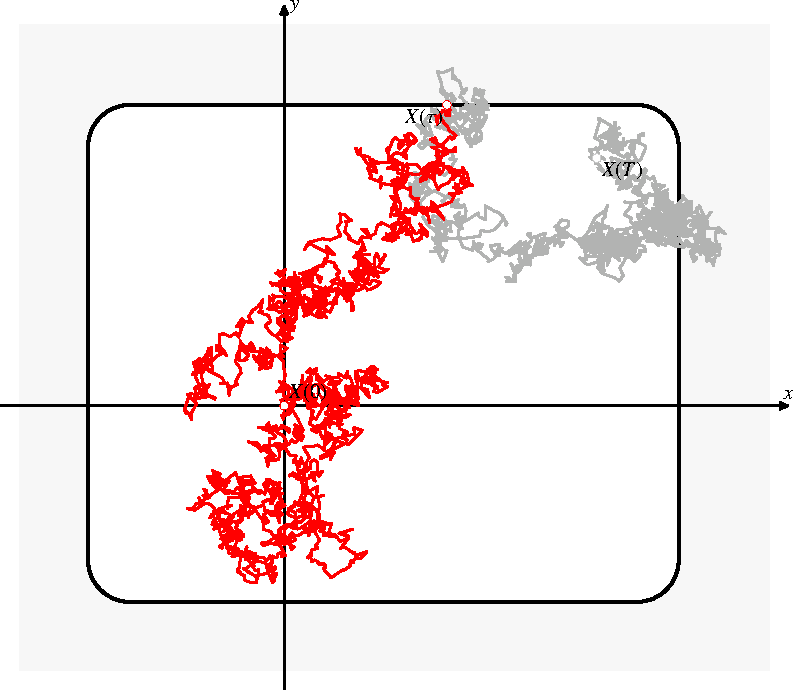
\includegraphics{chapters/images/stochastisch-2.pdf}
\caption{Brownsche Bewegung in zwei Dimension und Definition der
Stopzeit $\tau$, zu der der Pfad $X(t)$ das Gebiet verl"asst.
\label{stochastisch:pfad}}
\end{figure}

\begin{definition}
Sei $E$ eine beliebige offene oder abgeschlossene nicht leere Teilmenge
von $\mathbb R^n$.
Dann setzen wir
\[
\tau = \inf\{t\ge 0\;|\;X(t)\in E\},
\]
$\tau$ ist also die fr"uheste Zeit, zu der der Weg $X(t)$ die Menge $E$
erreicht.
\end{definition}

Die charakteristische Funktion
\[
\chi_{[0,\tau]}(t)=\begin{cases}
1\qquad\qquad&t\le \tau\\
0            &t>\tau
\end{cases}
\]
ist nat"urlich auch ein stochastischer Prozess, und damit auch 
$\chi_{[0,\tau]}G$.
Damit gelten die Regeln f"ur das It\^o-Integral aus
Satz~\ref{satz:ito-integral} auch f"ur diesen Prozess, jetzt allerdings
als Integrale mit oberer Grenze $\tau$ statt $T$.

\begin{hilfssatz}
Seien $G$ und $H$ auf $[0,T]$ quadratintegrierbare stochastische Prozesse
und $a,b\in\mathbb R$
\begin{compactenum}
\item
Das It\^o-Integral ist linear:
\begin{align*}
\int_0^\tau aG+bH\,dW
&=
\int_0^T a\chi_{[0,\tau]} G + b \chi_{[0,\tau]} H\,dW
=
a\int_0^T \chi_{[0,\tau]} G\,dW + b \int_0^T\chi_{[0,\tau]} H\,dW
\\
&=
a\int_0^\tau G\,dW + b \int_0^\tau H\,dW
\end{align*}
\item Der Erwartungswert des It\^o-Integrals ist
\[
E\biggl(\int_0^\tau G\,dW\biggr)
=
E\biggl(\int_0^T \chi_{[0,\tau]}G\,dW\biggr)
=
0.
\]
\item Die Varianz des It\^o-Integrals ist
\[
E\biggl(\biggl(\int_0^\tau G\,dW\biggr)^2\biggr)
=
E\biggl(\biggl(\int_0^T \chi_{[0,\tau]}G\,dW\biggr)^2\biggr)
=
E\biggl(\int_0^T\chi_{[0,\tau]}G^2\,dt\biggr)
=
E\biggl(\int_0^\tau G^2\,dt\biggr).
\]
\end{compactenum}
\end{hilfssatz}

Die It\^o-sche Kettenregel funktioniert auch f"ur $\tau$ als obere
Grenze f"ur die stochastischen Integrale.
Wenn also $X$ als stochastischer Prozess eine L"osung der stochastischen
Differentialgleichung (\ref{stochastisch:stopzeitdgl}) ist, dann gilt
nach der der It\^o-schen Kettenregel
\[
du(X,t)
=
\frac{\partial u}{\partial t}\,dt
+
\sum_{i=1}^n\frac{\partial u}{\partial x_i}\,dX_i
+
\frac12\sum_{i,j=1}^n\frac{\partial^2 u}{\partial x_i\partial x_j}
\sum_{k=1}^n b_{ik}b_{jk}\,dt.
\]
In integrierter Form bedeutet dies
\[
u(X(t),t)-u(X(0),0)
=
\int_0^t
\frac{\partial u}{\partial t}
+
\frac12\sum_{k=1}^nb_{ik}b_{jk}
\sum_{i,j=1}^n \frac{\partial^2u}{\partial x_i\,\partial x_j} \,ds
+
\int_0^t \operatorname{grad} u\cdot B\,dW.
\]
Und nat"urlich gelten diese Formeln auch dann, wenn man $t$ durch $\tau$
ersetzt.

Im Folgenden interessiert uns nur der Fall $b=0$, $b_{ik}=\delta_{ik}$
und Funktionen $u$, die nicht von der Zeit abh"angen.
Dann vereinfacht sich die Formel zu
\begin{equation}
u(X(t))-u(X(0))
=
\int_0^t \frac12\sum_{i=1}^n\frac{\partial^2 u}{\partial x_i^2}\,ds
=
\int_0^t \frac12\Delta u\,ds
\label{stochastisch:laplaceinkrement}
\end{equation}
Ausserdem ist in diesem Fall $X$ nichts anderes als eine Brownsche Bewegung,
$X=W$.

\subsection{Brownsche Bewegung und der Laplace-Operator}
Wir wenden die Formel (\ref{stochastisch:laplaceinkrement}) jetzt in
zwei Beispielen an.

\subsubsection{Zeit bis zum Verlassen eines Gebietes}
F"ur das erste Beispiel sei $U$ ein beschr"anktes Gebiet in
$\mathbb R^n$, und $u$ eine L"osung der partiellen Differentialgleichung
\begin{equation}
\begin{aligned}
-\frac12\Delta u&=1&\qquad&\text{in $U$}\\
               u&=0&      &\text{auf $\partial U$}
\end{aligned}
\label{stochastisch:hittingtime}
\end{equation}
Wir m"ochten die L"osung $u$ dazu verwenden, die Zeit $\tau_x$ zu berechnen,
zu der eine im Punkt $x\in U$ beginnende Brownsche Bewegung zum ersten
Mal das Gebiet $U$ verl"asst.
Die Formel (\ref{stochastische:laplaceinkrement}) liefert
\[
u(X(\tau_x))-u(X(0)) = \int_0^{\tau_x} \frac12\Delta u\,ds
\]
Da $u$ eine L"osung von (\ref{stochastisch:hittingtime}) ist, ist der 
Integrand auf der rechten Seite gleich $-1$:
\[
u(X(\tau_x))-u(X(0)) = -\int_0^{\tau_x} \,ds
\]
Da der Prozess $X$ zur Zeit $\tau_x$ den Rand des Gebietes "uberquert,
ist wegen der Randbedingung $u(X(\tau_x))=0$. 
Zusammen erhalten wir
\[
-u(X(0)) = -\tau_x.
\]
Nun interessiert uns aber nicht der Wert der Zufallsvariablen, sondern
nur deren Erwartungswert:
\[
E(\tau_x)=E(u(X(0)))=u(x).
\]
Die L"osung $u$ der Differentialgleichung (\ref{stochastisch:hittingtime})
gibt die erwartete Zeit an, bis eine bei $x$ beginnende Brownsche Bewegung 
das Gebiet $U$ verlassen hat.

\subsubsection{Charakterisierung von harmonischen Funktionen}
Sei wieder $U$ ein beschr"anktes Gebiet mit glattem Rand und
$g$ eine stetige Funktion auf $\partial U$.
Ausserdem sei $u$ eine harmonische Funktion in $U$ mit den Randwerten $g$, 
also eine L"osung der partiellen Differentialgleichung
\begin{equation}
\begin{aligned}
\Delta u&=0&\qquad&\text{in $U$}\\
       u&=g&      &\text{auf $\partial U$}
\end{aligned}
\label{stochastisch:harmonisch}
\end{equation}
Wir wollen (\ref{stochastisch:laplaceinkrement}) verwenden, die Funktion
$u$ zu charakterisieren.
Dazu sei wieder $\tau_x$ die Zeit, zu der eine im Punkt $x\in U$ beginnende
Brownsche Bewegung das Gebiet $U$ verl"asst.
Aus (\ref{stochastisch:laplaceinkrement}) folgt:
\[
u(X(\tau_x))-u(X(0))
=
\int_0^{\tau_x} \frac12\underbrace{\Delta u}_{\textstyle=0}\,ds=0.
\]
Zur Zeit $\tau_x$ ist $X(\tau_x)$ ein Randpunkt des Gebiets, der mit
der Randbedingung bestimmt werden kann, es folgt:
\[
u(X(0)) = g(X(\tau_x)).
\]
Wieder interessiert uns der einzelne Wert nicht, sondern der Erwartungswert:
\[
u(x)=E(g(X(\tau_x))).
\]
Den Wert im Punkt $x$ einer harmonischen Funktion mit Randwerten $g$
kann man wie folgt finden: man l"asst eine Brownsche Bewegung von $x$ 
aus laufen, bis sie den Rand "uberquert, und nimmt den Mittelwert
der derart erreichten Randwerte.

Aus dieser Charakterisierung der harmonischen Funktionen kann man
auch deren Mittelwerteigenschaft ableiten. 
Da die Brownsche Bewegung isotrop ist, muss sich im Zentrum
eines kugelf"ormigen Gebietes immer der gleiche Wert f"ur $u$
ergeben, selbst wenn man eine beliebige Drehung auf die Randwerte 
anwendet.
Also muss der Wert von $u(x)$ der Mittelwert der Werte
auf einer Kugel um den Punkt $x$ sein.

%
%
%
\section{Kalman-Filter\label{section:kalman}}
\rhead{Kalman-Filter}






\begin{appendices}
\chapter{Newton-Verfahren}
\lhead{Newton-Verfahren}
\rhead{}

\section{Nullstellen von Funktionen}
\rhead{Nullstellen von Funktionen}
\begin{figure}
\centering
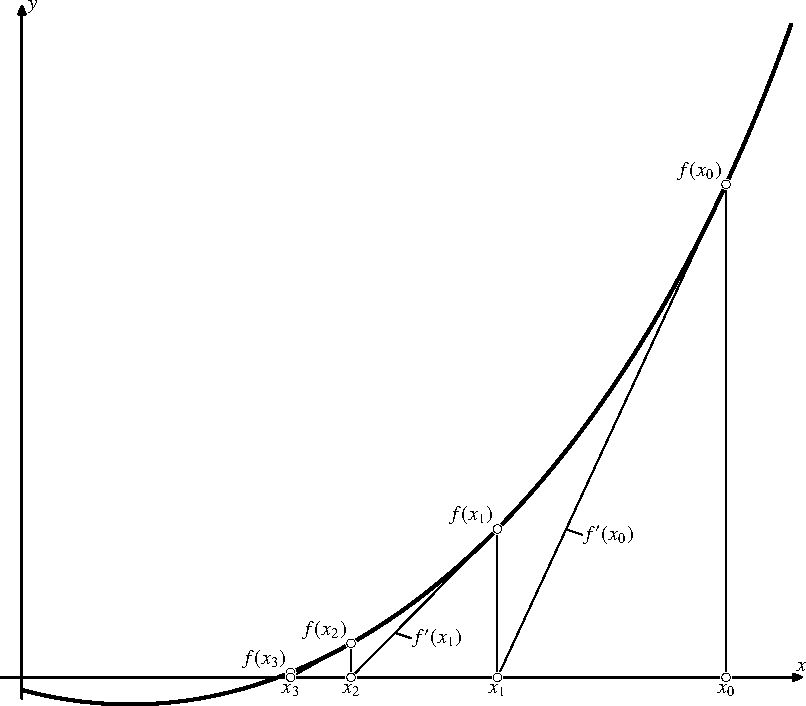
\includegraphics{chapters/images/randwert-2.pdf}
\caption{Bestimmung der Nullstelle einer Funktion $f(x)$ mit dem
Newton-Verfahren.
Die Approximation $x_{n+1}$ wird gefunden als Schnittpunkt der Tangente
im Punkt $(x_n,f(x_n))$ (mit Steigung $f'(x_n)$) mit der $x$-Achse.
\label{newton:graphik}}
\end{figure}
Das Ziel dieses Anhangs ist, die folgende Aufgabe numerisch zu l"osen:
\begin{aufgabe}
Gegen ist eine differenzierbar Funktion
$f\colon\mathbb R\to\mathbb R:x\mapsto f(x)$
und eine Zahl $y$ im Wertebereich von $f$.
Finde $\hat{x}\in\mathbb R$ so, dass $f(\hat{x})=y$.
\end{aufgabe}
Im allgemeinen kann man nicht davon ausgehen, dass sich eine L"osung der
Gleichung $f(x)=y$ in geschlossener Form finden l"asst.
Nur einige wenige Klassen von Gleichungen haben L"osungsformeln dieser Art.
Wir beschr"anken uns daher auf das Problem, eine Approximation f"ur die
L"osung zu bestimmen.

Indem wir statt der Funktion $f(x)$ die Funktion $x\mapsto g(x)=f(x)-y$
betrachten, k"onnen wir die gesuchte Zahl $x$ auch als L"osung der
Gleichung $g(x)=0$ finden:
\begin{equation}
f(x)=y
\qquad\qquad
\Rightarrow
\qquad\qquad
g(x)=f(x)-y = 0.
\label{newton:reduktion}
\end{equation}
Es gen"ugt also, ein L"osungsverfahren zu entwickeln f"ur die Aufgabe
\begin{aufgabe}
Gegen ist eine differenzierbar Funktion
$f\colon\mathbb R\to\mathbb R:x\mapsto f(x)$,
finde $\hat{x}\in\mathbb R$ so, dass $f(\hat{x})=0$.
\end{aufgabe}
Da wir nur eine numerische L"osung brauchen, versuchen wir sie dadurch
zu finden, dass wir eine Anfangssch"atzung $x_0$ wiederholt korrigieren,
bis der Fehler klein genug ist.
Es soll also eine Folge $x_0,x_1,x_2,\dots$ konstruiert werden, welche
gegen die L"osung $\hat{x}$ konvergiert.
Der Differenzenquotient ist eine Approximation f"ur die Steigung
$f'(x_n)$,
\begin{equation}
\frac{
f(x_{\mathstrut n+1})-f(x_{\mathstrut n})
}{
x_{\mathstrut n+1}-x_{\mathstrut n}
}
\simeq = f'(x_n).
\label{newton:pre}
\end{equation}
Wir m"ochten gerne, dass $f(x_{n+1})=0$ ist, und k"onnen (\ref{newton:pre})
unter dieser Annahme nach $x_{n+1}$ aufl"osen:
\begin{align*}
-f(x_n)
&\simeq
f'(x_n)\,(x_{\mathstrut n+1}-x_{\mathstrut n})
\\
x_{\mathstrut n}-\frac{f(x_n)}{f'(x_n)}
&\simeq x_{\mathstrut n+1}
\end{align*}
Damit haben wir ein L"osungsverfahren gefunden:
\begin{satz}[Newton]
Ist $f$ eine differenzierbare Funktion, deren Ableitung bei der Nullstelle
$\hat{x}$ nicht verschwindet, also $f(\hat{x})\ne 0$, und $x_0$ eine erste
Approximation f"ur $\hat{x}$, dann konvergiert die Folge
definiert durch die Rekursionsformel
\[
x_{n+1}=x_n-\frac{f(x_n)}{f'(x_n)},
\]
dann konvergiert $x_n$ gegen $\hat{x}$, falls $x_0$ nahe genug bei
$\hat{x}$ liegt.
\end{satz}

\begin{beispiel}
Man finde die Wurzel der Zahl $y$, d.~h.~man muss die Nullstellen
der Funktion $f(x)=x^2-y$ finden.
Das Newton-Verfahren ben"otigt die Ableitung von $f$, sie ist
$f'(x)=2x$, und konstruiert daraus die Folge
\begin{equation}
x_{n+1} = x_n - \frac{f(x_n)}{f'(x_n)}=x_n-\frac{x_n^2-y}{2x_n}
=
\frac{2x_n^2-x_n^2+y}{2x_n}
=
\frac12\biggl(x_n + \frac{y}{x_n}\biggr)
\label{newton:mittel}
\end{equation}
Die Quaratwurzel von $y$ erf"ullt nat"urlich
\[
\sqrt{y} = \frac12\biggl( \sqrt{y}+\frac{y}{\sqrt{y}}\biggr).
\]
Mit $x_n$ ist auch $y/x_n$ eine Approximation von $\sqrt{y}$.
Die neue Approximation $x_{n+1}$ ist das arithmetische Mittel der
beiden Approximationen $x_n$ und $y/x_n$ von $\sqrt{y}$.
Die Konvergenz dieser Folge ist sehr schnell, wie Tabelle~\ref{newton:sqrt2}
zeigt.
\begin{table}
\centering
\begin{tabular}{|>{$}r<{$}|>{$}r<{$}|}
\hline
n&x_n\\
\hline
0 &  2.00000000000000\\
1 &  1.50000000000000\\
2 &  1.\underline{41}666666666667\\
3 &  1.\underline{41421}568627451\\
4 &  1.\underline{41421356237}469\\
5 &  1.\underline{41421356237309}\\
6 &  1.\underline{41421356237309}\\
\hline
\end{tabular}
\caption{Approxmationen von $\sqrt{2}$ mit Hilfe des Newton-Algorithmus,
korrekte Stellen unterstrichen.
Die Anzahl korrekter Stellen verdoppelt sich in jedem Schritt.
\label{newton:sqrt2}}
\end{table}
In jedem Schritt verdoppelt sich die Anzahl korrekter Stellen.
Dies ist eine allgemeine Eigenschaft des Newton-Algorithmus, wie
in Abschnitt~\ref{section:newton:konvergenz} erkl"art wird.
\end{beispiel}

\section{Konvergenzgeschwindigkeit\label{section:newton:konvergenz}}

\section{L"osung von Vektorgleichungen\label{section:newton:vektor}}
\rhead{L"osung von Vektorgleichungen}
Wir m"ochten das Verfahren nun erweitern, so dass wir nicht nur eine
einzige Gleichung $f(x)=y$ nach $x$ aufl"osen k"onnen, wir m"ochten dazu 
f"ur ein Gleichungssystem von nichtlinearen Gleichungen
\begin{align*}
f_1(x_1,\dots,x_n)&=y_1\\
f_2(x_1,\dots,x_n)&=y_2\\
&\;\;\vdots\\
f_m(x_1,\dots,x_n)&=y_m
\end{align*}
ebenfalls in der Lage sein.
Wie bei einer einzigen Gleichung k"onnen wir das Problem reduzieren
auf das Finden von gleichzeitigen Nullstellen der Funktionen $g_i$ mit
\begin{align*}
g_1(x_1,\dots,x_n)&=f_1(x_1,\dots,x_n)-y_1=0\\
g_2(x_1,\dots,x_n)&=f_2(x_1,\dots,x_n)-y_2=0\\
&\;\;\vdots\\
g_m(x_1,\dots,x_n)&=f_m(x_1,\dots,x_n)-y_m=0.
\end{align*}










\chapter{Komplexe Zahlen}
\lhead{Komplexe Zahlen}
\rhead{}
Leonhard Euler sah die Zahlen $\sqrt{-1}$ noch als imagin"ar an,
also als ohne Gegenst"uck in der realen Welt.
Elektroingenieure verwenden komplexe Zahlen mit grossem Erfolg in ihren
Anwendungen, sie spielen aber vor allem die Rolle eines praktischen
Werkzeugs. Die Regeln, mit denen am Schluss solcher Rechnungen sichergestellt
wird, dass die Resultate reell sind, zeigen ausserdem, dass man alles auch
ohne komplexe Zahlen durchrechnen k"onnte, wenn auch wesentlich weniger
elegant.

In der Quantenmechanik geht es aber nicht mehr ohne komplexe Zahlen,
die physikalischen Gr"ossen selbst sind komplex. Es gibt zwar auch
hier wieder Regeln, die sicherstellen, dass Messresultate reell sind
(Operatoren m"ussen selbstadjungiert sein), aber sie erlauben nicht,
die ganze Quantenmechanik auf eine Art zu beschreiben, die ohne komplexe
Zahlen auskommt.

\section{Der K"orper \texorpdfstring{$\mathbb C$}{C} der komplexen Zahlen}
\rhead{Der K"orper $\mathbb C$}
In den reellen Zahlen $\mathbb R$ k"onnen alle Grundoperationen ausgef"uhrt
werden, es ist jedoch nicht m"oglich, die Quadratwurzeln aus negativen
Zahlen zu ziehen. Eine analoge Situation trifft man schon viel fr"uher.
In den nat"urlichen Zahlen $\mathbb N$ kann man zwar addieren und
multiplizieren, aber nicht subtrahieren.
F"ugt man die negativen Zahlen hinzu erh"alt man eine Menge $\mathbb Z$,
in der die Subtraktion uneingeschr"ankt m"oglich ist. Division ist aber
immer noch nur f"ur spezielle Divisoren m"oglich. F"ugt man jedoch die
Br"uche zu $\mathbb Z$ hinzu, erh"alt man die Menge der rationalen Zahlen
$\mathbb Q$, in der Division uneingeschr"ankt m"oglich ist.
Doch auch $\mathbb Q$ ist nicht vollst"andig, die Zahl $\sqrt{2}$ ist
keine rationale Zahl. Nat"urlich kann man $\sqrt{2}$ durch eine
Folge von Br"uchen $r_n\in\mathbb Q$ approximieren, doch der Grenzwert
dieser Folge $\lim_{n\to\infty}r_n=\sqrt{2}$ ist nicht in $\mathbb Q$.
F"ugt man jedoch alle Grenzwerte von konvergenten Folgen zu $\mathbb Q$
hinzu, erh"alt man die Menge $\mathbb R$ der reellen Zahlen, in der
auch beliebige Wurzeln von positiven Zahlen gezogen werden k"onnen,
oder andere Grenzwerte wie $\pi$, $e$, die Werte von $\sin x$ und $\cos x$
und weitere.

\subsection{Grundoperationen f"ur die komplexen Zahlen}
Nach analogem Muster k"onnen wir auch $\mathbb R$ erweitern, so dass auch
die Wurzeln aus negativen Zahlen bestimmt werden k"onnen. Es reicht
sogar, nur die Wurzel von $-1$ hinzuzuf"ugen, denn jede andere Wurzel
einer negativen Zahl ist $\sqrt{-a}=\sqrt{-1}\cdot\sqrt{\mathstrut a}$.
Euler hat die Bezeichnung $i=\sqrt{-1}$ f"ur die imagin"are Einheit eingef"uhrt.
Es gilt nat"urlich $i^2=-1$.
\index{imaginare Einheit@imagin\"are Einheit}

\begin{definition}
Die Menge $\mathbb C=\{a+bi\,|\,a,b\in\mathbb R\}$ heisst die Menge der
\index{komplexe Zahl}%
\index{C@$\mathbb C$}%
{\em komplexen Zahlen}. Die komplexe Zahl $z=a+bi$ hat
Realteil $\operatorname{Re}z=a$ und Imagin"arteil $\operatorname{Im}z=b$.
\index{Realteil}%
\index{Imaginarteil@Imagin\"arteil}%
\index{komplexe Zahl!Realteil}%
\index{komplexe Zahl!Imagin\"arteil}%
Die Rechenoperationen sind so zu verstehen, dass die Rechenregeln
der Algebra erhalten bleiben\footnote{Man nennt dies das Permanenz-Prinzip}.
\end{definition}

Die Rechenoperationen folgen aus der Definition:
\begin{align*}
(a+bi)+(c+di)&=(a+c)+(b+d)i\\
(a+bi)(c+di)&=ac-i^2bd+(ad+bc)i=ac-bd+(ad+bc)i
\end{align*}
Die Division stellt noch ein Problem dar. Hier hilft das Konzept der
konjugiert komplexen Zahl.
\index{komplexe Zahl!Division}%

\begin{definition}
Die Zahl $\bar z=a-bi$ heisst die zu $z=a+bi$ {\em konjugiert komplexe} Zahl.
\end{definition}
\index{konjugiert komplex}

Zun"achst kann man mit der konjugiert komplexen Zahl den Betrag einer
komplexen Zahl definieren:
\[
z\bar z=(a+bi)(a-bi)=a^2+abi-abi-i^2b^2=a^2+b^2\qquad\Rightarrow\qquad
|z|^2=z\bar z.
\]
Andererseits kann man damit auch komplexe Br"uche berechnen, indem man
mit der konjugiert komplexen Zahl des Nenners erweitert:
\begin{align*}
\frac{a+bi}{c+di}&=
\frac{a+bi}{c+di}
\cdot
\frac{c-di}{c-di}=\frac{ac+bd+(bc-ad)i}{c^2+d^2}
\end{align*}
Die komplexen Zahlen k"onnen in einer Ebene visualisert werden: 
Realteil und Imagin"arteil werden entlang orthogonaler Achsen abgetragen.
Die Punkte $(x,y)$ der $x$-$y$-Ebene entsprechen also der komplexen Zahl
$x+yi$ der komplexen Zahlenebene (Abbildung~\ref{skript:gaussebene}).
\begin{figure}
\centering
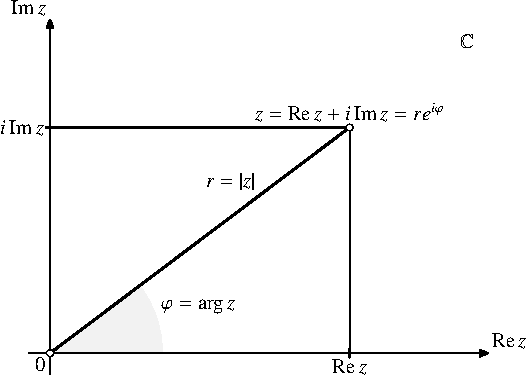
\includegraphics{chapters/images/komplexezahlen-1.pdf}
\caption{Komplexe Zahlenebene
\label{skript:gaussebene}}
\end{figure}
\index{Gauss-Ebene}%
\index{komplexe Zahlenebene}%

Mit Hilfe der komplexen Konjugation kann man den Real- and Imagin"arteil
einer komplexen Zahl $z=a+bi$ direkt ausdr"ucken:
\begin{align}
\operatorname{Re}z 
&=
a=\frac{(a+bi)+(a-bi)}2=\frac{z+\bar z}2
\label{skript:realteil-formel}
\\
\operatorname{Im}z
&=
b=\frac{(a+bi)-(a-bi)}{2i}=\frac{z-\bar z}{2i}.
\label{skript:imaginaerteil-formel}
\end{align}

\subsection{Polardarstellung}
\index{komplexe Zahl!Polardarstellung}
Die Darstellung der komplexen Zahlen als Punkte einer Ebene suggeriert
auch eine alternative Schreibweise.
Ein Punkt $z$ der komplexen Ebene kann auch charakterisiert werden mit Hilfe von
Polarkoordinaten, also durch seine Entfernung $r=|z|$ vom Nullpunkt,
und durch Polarwinkel zwischen der reellen Achse und der Richtung
zur komplexen Zahl. Der Polarwinkel heisst auch {\em Argument} $\operatorname{arg}z$,
\index{Argument}%
und es gilt
\[
\tan\operatorname{arg}z=\frac{\operatorname{Im}z}{\operatorname{Re}z}.
\]
\index{komplexe Zahl!Argument}
\index{komplexe Zahl!Betrag}
\index{komplexe Zahl!Multiplikation}
Die Multiplikation von komplexen Zahlen bekommt in der Polardarstellung
eine besondere Interpretation:
\begin{align*}
z_1z_2
&=
(r_1\cos\varphi_1+ir_1\sin\varphi_1) (r_2\cos\varphi_2+ir_2\sin\varphi_2)
\\
&=
r_1r_2(\cos\varphi_1+i\sin\varphi_1) (\cos\varphi_2+i\sin\varphi_2)
\\
&=
r_1r_2\bigl(
\cos\varphi_1\cos\varphi_2-\sin\varphi_1\sin\varphi_2 +
(\cos\varphi_1\sin\varphi_2+\sin\varphi_1\cos\varphi_2)i\bigr)
\\
&=
r_1r_2(\cos(\varphi_1+\varphi_2)+i\sin(\varphi_1+\varphi_2))
\\
\Rightarrow \operatorname{arg}z_1z_2&=\arg z_1 + \arg z_2
\end{align*}
Die Multiplikation zweier komplexen Zahlen entspricht also der
Multiplikation der Betr"age, und der Addition der Argumente.

Wir versuchen jetzt, die Werte der Exponentialfunktion zu $e^z$ zu
bestimmen.
Die Exponentialgesetze sollten auch weiterhin gelten.
Sei also $z=a+bi$, dann ist
\[
e^z=e^{a+bi}=e^a\cdot e^{bi}.
\]
Die Exponentialfunktion reeller Zahlen ist bereits wohlbekannt, es muss
also nur noch untersucht werden, welche Bedeutung $e^{bi}$ hat.

Betrachten wir die Funktion $f(t)= e^{it}$. Die Ableitungen von $f$ sind
\begin{align}
f'(t)&=ie^{it}=if(t)\notag\\
f''(t)&=-f(t).\label{skript:exp-dgl}
\end{align}
Die Funktion $f$ muss also eine L"osung der Differentialgleichung
(\ref{skript:exp-dgl}) sein, welche die Anfangsbedingungen $f(0)=1$ und
$f'(0)=if(0)=i$ erf"ullen muss.
Doch die Differentialgleichung (\ref{skript:exp-dgl}) hat die L"osungen
\[
f(t)=a\cos t+b\sin t.
\]
Setzt man die Anfangsbedingungen ein, findet man
\begin{align*}
f(0)&=1&\Rightarrow&&a&=1\\
f'(0)&=1&\Rightarrow&&b&=i,
\end{align*}
so dass wir jetzt $e^{it}$ ausrechnen k"onnen:
\begin{satz}[Euler]
\begin{align}
e^{it}=\cos t+i\sin t.
\label{skript:euler-formula}
\end{align}
\end{satz}
\index{Euler-Formel}%

Die komplexe Konjugation kehrt das Vorzeichen des Imagin"arteils um, also 
von $\sin t$. Da $\sin t$ eine ungerade Funktion ist, ist dies gleichbedeuten
damit, das Vorzeichen von $t$ zu kehren: $\overline{e^{it}}=e^{-it}$.

Mit der Eulerschen Formel sind wir jetzt auch in der Lage, den Zusammenhang
zwischen einer komplexen Zahl und ihrem Betrag und Argument sehr pr"agnant
auszudr"ucken:
\[
z=|r|\cdot e^{i\operatorname{arg}z}.
\]
Die Real- und Imagin"arteile von $e^{it}$ sind $\cos t$ und $\sin t$,
wir k"onnen sie auch mit den Formeln (\ref{skript:realteil-formel}) und
(\ref{skript:imaginaerteil-formel}) ausdr"ucken:
\begin{align*}
\cos t
&=
\operatorname{Re}e^{it}
=
\frac{e^{it}+\overline{e^{it}}}2
=
\frac{e^{it}+e^{-it}}2
\\
\sin t
&=
\operatorname{Im}e^{it}=\frac{e^{it}-e^{-it}}{2i}.
\end{align*}

\subsection{Matrixdarstellung der komplexen Zahlen\label{subsection:matrixdarstellung}}
\index{komplexe Zahl!Matrixdarstellung}
Die Algebra der komplexen Zahlen kann man auch als eine Algebra von Matrizen
schreiben. Dazu betrachten wir die Abbildung
\[
\varphi\colon
\mathbb C\to M_2(\mathbb R):
a+bi\mapsto\begin{pmatrix}a&b\\-b&a\end{pmatrix}
\]
Die imagin"are Einheit $i$ wird von $\varphi$ auf die Matrix
\[
\varphi(i)=J=\begin{pmatrix}0&1\\-1&0\end{pmatrix}
\]
abgebildet. Man kann nachrechnen, dass $J^2=-E$, und dass die Rechenregeln
f"ur die komplexen Zahlen durch die Abbildung $\varphi$ in die Rechenregeln
f"ur Matrizen transformiert werden.
Wir illustrieren dies f"ur die Multiplikation:
\[
\begin{aligned}
&(a+bi)(c+di)&&\mapsto&
&\begin{pmatrix}a&b\\-b&a\end{pmatrix}
\begin{pmatrix}c&d\\-d&c\end{pmatrix}
\\
&(ac-bd) + i(ad-bc)&&\mapsto&
&=\begin{pmatrix}
ac-bd&ad-bc\\
-ad+bc&ac-bd
\end{pmatrix}
\end{aligned}
\]
In dieser Darstellung kann man auch $e^{Jt}$ ausrechnen, indem man $Jt$ in
die Taylorreihe von $e^x$ einsetzt
\begin{align}
e^{Jt}
&=
E + tJ + \frac{t^2}{2!} J^2 + \frac{t^3}{3!} J^3 + \frac{t^4}{4!} J^4
 + \frac{t^5}{5!} J^5 + \frac{t^6}{6!} J^6 + \frac{t^7}{7!} J^7 + \dots
\notag
\\
&=
E + tJ - \frac{t^2}{2!} E - \frac{t^3}{3!} J + \frac{t^4}{4!} E
 - \frac{t^5}{5!} J - \frac{t^6}{6!} E + \frac{t^7}{7!} J + \dots
\notag
\\
&=\biggl(1 - \frac{t^2}{2!} + \frac{t^4}{4!} - \frac{t^6}{6!} + \dots\biggr) E
+ \biggl(t - \frac{t^3}{3!} + \frac{t^5}{5!} - \frac{t^7}{7!} + \dots\biggr) J
= E \cos t + J \sin t.
\label{skript:eulermatrixdarstellung}
\end{align}
Die Eulerformel (\ref{skript:euler-formula}) l"asst sich also auch in der
Matrixdarstellung der komplexen Zahlen wiedergewinnen.

\section{Komplexe Matrizen}
\rhead{Komplexe Matrizen}
\index{Matrix!komplex}%
Die Lineare Algebra im Bachelor wird typischerweise nur in den
reellen Zahlen entwickelt, der einzige untersuchte Vektorraum ist
der Raum $\mathbb R^n$ der reellen $n$-dimensionalen Vektoren.
F"ur die Quantenmechanik ben"otigen wir aber auch Vektoren mit
komplexen Komponenten. Der $n$-dimensionale komplese Vektorraum
$\mathbb C^n$ ist die Menge
\[
\left\{\left.\begin{pmatrix}c_1\\\vdots\\c_n\end{pmatrix}\,\right|
c_i\in\mathbb C\right\},
\]
mit der komponentenweisen Addition und der Multiplikation mit einer
komplexen Zahl. Nichts an der elementaren linearen Algebra hat besondere
Eigenschaften der reellen Zahlen verwendet, die nicht auch die komplexen
Zahlen haben. Der Gauss-Algorithmus, die Konstruktion der Determinanten,
ja sogar der grundlegende Algorithmus zur L"osung des Eigenwertprobems
funktioniert genau gleich auch f"ur komplexe Matrizen. Nur im Bereich
des Skalarproduktes sind minimale Modifikationen notwendig.

\subsection{Skalarprodukt f"ur komplexe Vektorr"aume}
In der linearen Algebra im ersten Semester wird das Skalarprodukt
geometrisch mit Hilfe der Projektion eingef"uhrt.
Eine solche Konstruktion ist f"ur komplexe Vektoren nicht m"oglich,
weil es keine anschauliche komplexe Geometrie gibt.

\subsubsection{Komplexes Skalarprodukt}
Um ein komplexes Skalarprodukt zu bekommen, gehen wir daher von den
algebraischen Eingeschaften des Skalarproduktes aus:
\begin{compactenum}
\item Das Skalarprodukt $(u,v)$ von komplexen Vektoren $u$ und $v$ ist linear
in $v$.
\item $(u,u) > 0$ falls $u\ne 0$.
\item Falls $(u,v)\in\mathbb R$, dann ist $(u,v)=(v,u)$.
\end{compactenum}
Diese Eigenschaften m"ussen auch f"ur ein komplexes Skalarprodukt gelten.
Wir zeigen, dass diese Eigenschaften auch ein komplexes Skalarprodukt 
weitgehend festlegt.

Zun"achst stellen wir fest, dass wir nicht erwarten k"onnen, dass
ein Skalarprodukt linear sein kann.
Betrachten wir dazu einen eindimensionalen Vektorraum $\mathbb C^1$.
Vektoren sind hier nur komplexe Zahlen, und ein Produkt, welches
linear in beiden Faktoren ist, ist von der Form $(u,v)=uv$. Dann ist
aber $(u,u)=u^2$, aber $u^2$ kann auch negativ sein, zum Beispiel f"ur $u=i$.
Das einzige Produkt, welches immer positiv ist, ist $(u,v)=\bar uv$.
Dieses Produkt ist aber nicht linear im Faktor $u$:
\[
(\lambda u,v)=\overline{(\lambda u)}v=\bar\lambda (\bar uv)=\bar\lambda (u,v).
\]
Wir m"ussen also von einem komplexen Skalarprodukt verlangen, dass es
\index{konjugiert linear}
im ersten Faktor {\em konjugiert linear} ist:
\[
(\lambda u,v)=\bar\lambda(u,v)
\]
Eine Funktion von zwei Vektoren, welche linear im zweiten Vektor ist
und konjugiert linear im ersten heisst {\em sesquilinear}.
\index{sesquilinear}%
\index{Sesquilinearform}%

Sei jetzt also $(\,\cdot\,|\,\cdot\,)$ eine Sesquilinearform.
Wir setzen $\lambda = 1/(u,v)$, dann gilt
$(u,\lambda v)$ reell ist. Dann gilt
\begin{align*}
1&=\lambda (u,v)=(u,\lambda v)=(\lambda v,u)=\bar\lambda(v,u)
&
&\Rightarrow&
\frac1{(\bar\lambda)}&=(v,u)
&
&\Rightarrow&
\overline{(u,v)}&=(v,u).
\end{align*}
Vertauschung der Faktoren ist also gleichbedeutend mit komplexer Konjugation
des Wertes des Skalarproduktes. Man nennt eine Funktion von zwei komplexen
Vektoren {\em hermitesch}, wenn $(u,v)=\overline{(v,u)}$ gilt.
\index{hermitesch}
\index{Matrix!hermitesch}

Eine hermitesche Sesquilinearform heisst {\em positiv definit}, wenn
\index{positiv definit}
f"ur jeden Vektor $u\ne 0$ gilt $(u,u)>0$. Diese Eigenschaft stellt
sicher, dass $(u,u)$ sinnvoll als die ``L"ange'' eines Vektors interpretiert
werden kann.

\begin{definition}
Ein komplexes Skalarprodukt ist eine positiv definite,
hermitesche Sesquilinearform.
\end{definition}
\index{Skalarprodukt!komplexes}

Das einfachste Beispiel eines komplexen Skalarproduktes ist
\[
(u,v)=\sum_i \bar u_iv_i.
\]
Die Standardbasisvektoren sind auch in diesem Skalarprodukt
orthonormiert.

%
% Adjungierte Matrix
%
\subsubsection{Adjungierte Matrix}
\index{adjungiert}
\index{Matrix!adjungiert}
\index{Abbildung!linear}
In den reellen Vektorr"aumen konnte man zu einer linearen $A$ immer
eine lineare Abbildung $A^t$ finden mit der Eigenschaft
$(u,Av)=(A^tu,v)$. Mit Hilfe der Standardbasisvektoren konnte
man auch ausrechnen, was dies f"ur die Matrizen von $A$ bedeutet:
\[
(e_i,A^te_j),
=
(A^te_j, e_i)
=
(e_j,Ae_i)=a_{ji}
\]
d.~h.~die Matrix von $A^t$ ist die transponierte Matrix von $A$.
Eine symmetrische Matrix war eine, die sich beim Transponieren nicht
"andert, also $A^t=A$.

Dasselbe kann man jetzt auch f"ur ein komplexes Skalarprodukt
versuchen. Zu einer komplexen Matrix $A$ ist also eine neue
Matrix $A^*$ gesucht, mit der Eigenschaft, $(A^*u,v)=(u,Av)$ f"ur 
jedes Paar von Vektoren $u$ und $v$. F"ur die Standardbasisvektoren
gilt dann
\[
(e_i,A^*e_j),
=
\overline{(A^*e_j, e_i)}
=
\overline{(e_j,Ae_i)}=\overline{a_{ji}},
\]
die Matrix von $A^*$ ist also nicht nur transponiert, sondern auch komplex
konjugiert. Hat $A$ die Ma\-trix\-e\-le\-men\-te $a_{ij}$ dann nennt man
die Matrix $A^*$ mit den Matrixelementen $\bar a_{ji}$ die
adjungierte Matrix. Eine Matrix, die sich beim Adjungieren nicht
"andert, heisst {\em selbstadjungiert}.
\index{Matrix!selbstadjungiert}
\index{selbstadjungiert}

Die Rechenregeln f"ur die adjungierte Matrix sind ganz "ahnlich wie
f"ur die Transposition:
\index{Transposition}%
\[
\begin{aligned}
(\lambda A)^*&=\bar\lambda A^*,
&
(A+B)^*&=A^*+B^*,
&
(AB)^*=B^*A^*.
\end{aligned}
\]
Man beachte, dass $A\mapsto A^*$ nicht linear ist.

\subsubsection{Unit"are Matrizen}
\index{unitar@unit\"ar}
Matrizen, die in reellen Vektorr"aumen das Skalarprodukt nicht "andern,
heissen orthogonal. Sie sind charakterisiert durch die Eigenschaft
\index{Matrix!orthogonal}%
\index{orthogonal}%
$(Ox,Oy)=(x,y)$, woraus sich mit Hilfe der Transposition ergibt:
\[
(Ox,Oy)=(O^tOx,y)=(x,y)\qquad\Rightarrow\qquad O^tO=E,
\]
woraus man weiter ablesen kann, dass bei orthogonalen Matrizen
die transponierte Matrix mit der invertierten Matrix zusammenf"allt.

F"ur komplexen Vekoren kann man wieder nach den Matrizen fragen, die das
komplexe Skalarprodukt nicht ver"andern. Eine Matrix $U$ hat diese
Eigenschaft, wenn
\[
(Ux,Uv)=(U^*Ux,y)=(x,y)\;\forall x,y
\qquad\Rightarrow\qquad
U^*U=E
\]
gilt,
eine solche Matrix heisst {\em unit"ar}. 
\index{unitar@unit\"ar}
\index{Matrix!unit\"ar}

F"ur reelle Matrizen $A$ ist $A^t=A^*$, also sind orthogonale Matrizen
auch unit"ar.

\begin{beispiel}
Die unit"aren $1\times 1$-Matrizen sind komplexe Zahlen $z$, welche
die zus"atzliche Bedingung $\bar zz=1$ erf"ullen m"ussen.
Die Menge der unit"aren $1\times 1$-Matrizen ist also
\[
U(1)=\left\{ z\in\mathbb C\,|\, |z|=1
\right\}.
\]
In der Quantenmechanik k"onnen Zustandsvektoren in der Regel nur bis auf
einen komplexen Faktor vom Betrag $1$, also bis auf ein Element
von $U(1)$ festgelegt werden.
Man spricht oft von ``bedeutungslosen'' Phasenfaktoren.
\end{beispiel}

\subsubsection{Die spezielle unit"are Gruppe $\operatorname{SU}(2)$}
\index{spezielle unit\"are Gruppe}
\index{SU(2)}
Wir betrachten Matrizen der Form
\begin{equation}
U=
\begin{pmatrix}
a&b\\-\bar b&\bar a
\end{pmatrix}
\label{skript:su2form}
\end{equation}
mit der zus"atzlichen Bedingung $|a|^2 + |b|^2=1$. Sie erf"ullen
\begin{align*}
U^*U
&=
\begin{pmatrix}
\bar a&-b\\\bar b&a
\end{pmatrix}
\begin{pmatrix}
a&b\\-\bar b&\bar a
\end{pmatrix}
=
\begin{pmatrix}
\bar aa+b\bar b & \bar ab-b\bar a\\
\bar ba-a\bar b & \bar bb+a\bar a
\end{pmatrix}
=
E
\\
\det(U)&=\left|
\begin{matrix}
a&b\\-\bar b&\bar a
\end{matrix}
\right|
=
a\bar a+\bar bb = |a|^2 + |b|^2=1.
\end{align*}
Solche Matrizen sind also nicht nur unit"ar, sondern haben auch Determinante 1.
Multipliziert man zwei Matrizen der Form (\ref{skript:su2form}),
wird das Produkt auch wieder Determinante 1 haben, aber es ist nicht klar,
dass es sich in der Form (\ref{skript:su2form}) schreiben l"asst.
Daher rechnen wir das Produkt aus, wir erhalten
\begin{align*}
\begin{pmatrix}  a                        & b                      \\
                 -\bar b                  & \bar a                 \end{pmatrix}
\begin{pmatrix}  c                        & d                      \\
                 -\bar d                  & \bar c                 \end{pmatrix}
&=
\begin{pmatrix}  ac-b\bar d               & ab+b\bar c             \\
                 -\bar bc-\bar a\bar d    & -\bar bd +\bar a\bar c \end{pmatrix}
=
\begin{pmatrix}  ac-b\bar d               & ab+b\bar c             \\
                 -(\overline{ab+b\bar c}) & \overline{ac-b\bar d}  \end{pmatrix}
.
\end{align*}
Das Produkt zweier Matrizen der Form (\ref{skript:su2form}) ist also wieder eine
Matrix der Form (\ref{skript:su2form}).
Die Menge dieser Matrizen ist demzufolge abgeschlossen unter
Matrixmultiplikation und Bildung der Inversen.
Man nennt diese Matrizen die Gruppe der speziellen unit"aren Matrizen:
\[
\operatorname{SU}(2)=\left\{
\left.
\begin{pmatrix}
a&b\\-\bar b&\bar a
\end{pmatrix}
\,
\right|
\,
a,b\in\mathbb C\wedge
|a|^2+|b|^2=1
\right\}.
\]
Die Gruppe $\operatorname{SU}(2)$ spielt bei der Analyse des Elektronenspins
eine wichtige Rolle.

Die Gruppe $\operatorname{SU}(2)$ ist eine Teilmenge der Menge der komplexen
$2\times 2$-Matrizen:
\[
\operatorname{SU}(2)
\subset
V=
\left\{
\left.
\begin{pmatrix}a&b\\-\bar b&\bar a\end{pmatrix}\,
\right|
a,b\in\mathbb C^2
\right\}
\subset
M_2(\mathbb C)
=\left\{
\left.
\begin{pmatrix}
a&b\\c&d
\end{pmatrix}
\,
\right|
\, a,b,c,d\in\mathbb C
\right\}
\]
Wir untersuchen die Menge $V$ etwas genauer.
Zun"achst k"onnen wir $V$ als zweidimensionalen komplexen Vektorraum
betrachten wie $\mathbb C^2$.
Als reeller Vektorraum betrachtet ist $V$ ein vierdimensionaler
reeller Vektorraum. Die Abbildung
\[
\mathbb R^4\to\mathbb C^2\to V
:
\begin{pmatrix}x_1\\x_2\\x_3\\x_4\end{pmatrix}\mapsto
\begin{pmatrix}x_1+ix_2\\x_3+ix_4\end{pmatrix}\mapsto
\begin{pmatrix} x_1+ix_2 & x_3+ix_4 \\
               -x_3+ix_4 & x_1-ix_2 \end{pmatrix}
\]
ist eine Bijektion zwischen $\mathbb R^4$, $\mathbb C^2$ und $V$.
Auch geometrisch ist $\mathbb C^2=\mathbb C\times \mathbb C$ das Produkt
von zwei Ebenen, hat also eine vierdimensionale Geometrie.
Darin ist $\operatorname{SU}(2)$ die Teilmenge der vierdimensionalen Vektoren,
und zwar derjenigen f"ur die gilt
\[
1
=
|a|^2+|b|^2
= 
x_1^2 + x_2^2 + x_3^2 + x_4^2,
\]
das sind die Vektoren von $\mathbb R^4$ mit L"ange $1$.
Geometrisch ist $\operatorname{SU}(2)$ also eine dreidimensionale Kugel
eingebettet in in einen vierdimensionalen Raum.

\subsubsection{Spur und Determinante}
Spur und Determinate k"onnen samt all ihren Rechenregeln sofort auf
komplexe Matrizen "ubertragen werden.
F"ur den Adjunktionsoperator finden wir die Rechenregeln
\[
\begin{aligned}
\det A^*&= \overline{\det A^t}=\overline{\det A},
&&\text{und}&
\operatorname{tr} A^*&=\overline{\operatorname{tr}A}.
\end{aligned}
\]
F"ur selbstadjungierte Matrizen kann man schliessen, dass sowohl
die Determinante wie auch die Spur von $A$ reell sein m"ussen.

In den komplexen Zahlen hat jedes Polynom $n$-ten Grades $n$ Nullstellen.
Daher k"onnen wir das charakteristische Polynom immer ausschreiben als
\begin{align*}
\det(A-\lambda E)
&=
(-1)^n (\lambda-\lambda_1)\dots(\lambda-\lambda_n)
\\
&=
(-1)^n(\lambda^n -(\lambda_1+\dots+\lambda_n)\lambda^{n-1}+\dots
+(-1)^n\lambda_1\dots\lambda_n
\\
&=
(-1)^n(\lambda^n - \operatorname{tr}A\lambda^{n-1}+\dots + (-1)^n\det A)
\end{align*}
Daraus k"onnen wir auch eine Formel f"ur $\det(E+tA)$ ableiten:
\begin{align}
\det(E+tA)
&=
(-t)^n\det\biggl(A-\frac1tE\biggr)
=
t^n\biggl(
\frac1{t^n}+\frac1{t^{n-1}}\operatorname{tr}A+\dots+\det A
\biggr)
\notag
\\
&=
1+t\operatorname{tr}A+\dots+t^n\operatorname{det}A
\label{skript:detandtrace}
\end{align}

%
% Eigenwertproblem fuer komplexe Matrizen
%
\subsection{Eigenwertproblem f"ur komplexe Matrizen}
\subsubsection{Definition}
Ein Vektor $v\ne 0$ heisst {\em Eigenvektor zum Eigenwert} $\lambda$ einer
\index{Eigenwert}
\index{Eigenvektor}
Matrix $A$, wenn $Av=\lambda v$ gilt. Diese Definition ist auch f"ur
komplexe Matrizen g"ultig, ebenso funktioniert der Standardalgorithmus
f"ur die L"osung des Eigenwertproblems nach wie vor:
\begin{enumerate}
\item Finde die Nullstellen der charakteristischen Gleichung
$\det(A-\lambda E)=0$.
\item F"ur jede Nullstelle $\lambda_i$, finde Eigenvektoren
durch L"osung des Gleichungssystems $(A-\lambda_i E)v=0$.
\end{enumerate}
Der wesentliche Unterschied ist jedoch, dass in den komplexen
Zahlen ein Polynom vom Grade $n$ immer $n$ Nullstellen hat.
Die bei reellen Matrizen vorkommende Situation, dass weniger
als $n$ reelle Nullstellen existieren, und daher nicht gen"ugend
Eigenvektoren f"ur eine Eigenvektorbasis gefunden werden k"onnen,
tritt also bei komplexen Matrizen seltener auf.

\subsubsection{Selbstadjungierte Matrizen}
Der quantenmechanische Formalismus beschreibt physikalische Gr"ossen
als selbstadjungierte Matrizen. Die m"oglichen Werte einer solchen Gr"osse
sind die Eigenwerte der Matrix, und es muss sichergestellt werden,
dass keine komplexen Eigenwerte auftreten k"onnen.

\begin{satz}
\label{skript:ewreell}
Die Eigenwerte einer selbstadjungierten Matrix sind reell.
\end{satz}
\begin{proof}[Beweis]
Sei $v$ ein Eigenvektor zum Eigenwert $\lambda$ einer selbstadjungierten
Matrix $A$. Dann gilt
\begin{align*}
(v,Av)
&=
\lambda(v,v)
\\
&=(Av,v)=(\lambda v,v)=\bar\lambda(v,v)
\\
\Rightarrow \lambda&=\bar\lambda,
\end{align*}
also ist $\lambda\in\mathbb R$.
\end{proof}

Bei reellen Matrizen hat sich gezeigt, dass symmetrische Matrizen immer
diagonalisierbar sind. Dies gilt auch f"ur selbstadjungierte Matrizen
in komplexen Vektorr"aumen:

\begin{satz}
\label{skript:evorthogonal}
Eine selbstadjungierte Matrix ist diagonalisierbar und die Eigenvektoren zu
verschiedenen Eigenwerten sind orthogonal.
\end{satz}

\begin{proof}[Beweis]
Wir beweisen nur die Orthogonalit"at von Eigenvektoren zu verschiedenen 
Eigenwerten. Seien also $v_1,v_2$ Eigenvektoren zu zwei verschiedenen
Eigenwerten $\lambda_1,\lambda_2$. Die beiden Eigenwerte sind nach
Satz~\ref{skript:ewreell} reell. Dann gilt
\begin{align*}
(v_1,Av_2)&=\lambda_2(v_1,v_2)
\\
          &=(Av_1,v_2)=\bar\lambda_1(v_1,v_2)=\lambda_1(v_1,v_2)
\\
\Rightarrow\quad
(\lambda_1-\lambda_2)(v_2,v_2)&=0
\end{align*}
Die letzte Gleichung kann wegen $\lambda_1\ne\lambda_2$ nur wahr sein,
wenn $(v_1,v_2)=0$, die Vektoren $v_1$ und $v_2$ m"ussen also orthogonal sein.
\end{proof}

%
% Lie Algebrean
%
\section{Lie-Algebren}
\rhead{Lie-Algebren}
\index{Lie-Algebra}
Die invertierbaren Matrizen $\operatorname{GL}(n)$ k"onnen weiter
unterteilt werden in invertierbare Matrizen mit zus"atzlichen
Eigenschaften wie Orthogonalit"at oder spezielle Werte der Determinanten.
Allerdings bildet die Menge der invertierbaren Matrizen keinen
Vektorraum: man kann sie nicht addieren oder mit beliebigen Zahlen
multiplizeren, weil die Invertierbarkeit oder eine der zus"atzlichen
Eigenschaften dabei verloren gehen kann. Diese Matrizen sind 
daher nicht geeignet als Observable in der Quantenmechanik.

Ist eine Matrix $A$ invertierbar, dann wird auch eine Matrix, deren
Matrixelemente nur wenig von $A$ abweichen, invertierbar sein.
Insbesondere werden die Matrizen der Form $E+tA$ invertierbar sein,
wenn nur $t$ klein genug ist. Dies ist ein "Ubergang zu einer 
infinitesimalen Transformation $A$.

Wie m"ussen die Rechenoperationen beim "Ubergang zu infinitesimalen
Transformationen "ubersetzt werden?
Wegen
\[
(E+tA)(E+tB)=E+(A+B)t + t^2AB\simeq E+(A+B)t
\]
wird beim "Ubergang zur infinitesimalen Transformation aus dem Produkt
der Matrizen die Summe von Matrizen, und aus der Inversen wird die Negation.

Betrachten wir die Bedingung Orthogonalit\"at
\[
E=
(E+\varepsilon A)^t(E+\varepsilon A)
=
E+\varepsilon (A^t+A) + \dots
\qquad
\Rightarrow
\qquad
A^t=-A.
\]
Die infinitesimale Versionen von orthogonalen Matrizen sind also
antisymmetrische Matrizen.
\index{antihermitsche Matrix}
\index{Matrix!antihermitesch}
Analog sind die infinitesimalen Versionen von unit"aren Matrizen
antihermitesch.

Die Matrizenmultiplikation ist nicht kommutativ.
Diese Tatsache kann ausgenutzt werde, um den
Matrizenmengen eine zus"atzliche algebraische Struktur zu geben.
\index{Kommutator}%
Der Kommutator $[A,B]=AB-BA$ zweier Matrizen $A$ und $B$ erh"alt
die oben genannten Eigenschaften. Ist $A$ antisymmetrisch, dann
ist auch $[A,B]$ auch antisymmetrisch:
\[
[A,B]^t
=
(AB-BA)^t
=
B^tA^t-A^tB^t
=
(-B)(-A)-(-A)(-B)
=
-(AB-BA)
=
-[A,B].
\]
\index{Jacobi-Identit\"at!f\"ur Operatoren}%
Die Kommutatorklammer hat aber auch noch eine zus"atzliche Eigenschaft,
f"ur drei Matrixen $A$, $B$ und $C$ gilt n"amlich die sogenannte
Jacobi-Identit"at:
\begin{equation}
[A,[B, C]]
+
[B,[C, A]]
+
[C,[A, B]]
=
0
\label{skript:jacobi}
\end{equation}
Um dies einzusehen rechnen wir die Kommutatoren aus:
\begin{align*}
&
[A,[B, C]]
+
[B,[C, A]]
+
[C,[A, B]]
\\
&=
A(BC-CB)-(BC-CB)A
+
B(CA-AC)-(CA-AC)B
+
C(AB-BA)-(AB-BA)C
\\
&=
ABC-ACB-BCA+CBA
+
BCA-BAC-CAB+ACB
+
CAB-CBA-ABC+BAC
\\
&=0
\end{align*}
Ein Vektorraum mit einer antisymmetrischen, bilinearen Abbildung
$[\,\cdot\,,\,\cdot\,]$,
welche die Jacobi-Identit"at (\ref{skript:jacobi}) erf"ullt, heisst eine
{\em Lie-Algebra}.
\index{Lie-Algebra}%
So wie der Hamilton-Operator als Erzeuger der Zeitentwicklung das
leichter zu manipulierende Objekt ist, ist die Liealgebra zu einer
Transformationsgruppe wie $\operatorname{SU}(2)$ besser geeignet
zur Beschreibung von Transformationen, und wird daher von Physikern
vorgezogen.

\begin{beispiel}
\index{SO(3)}
Zur Gruppe $\operatorname{SO}(3)$ der Drehmatrizen geh"ort die Lie-Algebra
$\operatorname{so}(3)$ der antisymmetrischen $3\times 3$-Matrizen.
Solche Matrizen haben die Form
\[
\Omega
=
\begin{pmatrix}
    0    & \omega_3&-\omega_2\\
-\omega_3&   0     & \omega_1\\
 \omega_2&-\omega_1&    0
\end{pmatrix}
\]
Der Vektorraum $\operatorname{so}(3)$ ist also dreidimensional.

Die Wirkung von $E+t\Omega$ auf einem Vektor $x$ ist
\[
(E+t\Omega)
\begin{pmatrix}x_1\\x_2\\x_3\end{pmatrix}
=
\begin{pmatrix}
    1     & t\omega_3&-t\omega_2\\
-t\omega_3&   1      & t\omega_1\\
 t\omega_2&-t\omega_1&    1
\end{pmatrix}
\begin{pmatrix}x_1\\x_2\\x_3\end{pmatrix}
=
\begin{pmatrix}
x_1-t(-\omega_3x_2+\omega_2x_3)\\
x_2-t( \omega_3x_1-\omega_1x_3)\\
x_3-t(-\omega_2x_1+\omega_1x_2)
\end{pmatrix}
=
x- t\begin{pmatrix}\omega_1\\\omega_2\\\omega_3\end{pmatrix}\times x
=
x+ tx\times \omega.
\]
Die Matrix $\Omega$ ist als die infinitesimale Version einer Drehung
um die Achse $\omega$.

Wir k"onnen die Analogie zwischen Matrizen in $\operatorname{so}(3)$ und
Vektoren in $\mathbb R^3$ noch etwas weiter treiben. Zu jedem Vektor
in $\mathbb R^3$ konstruieren wir eine Matrix in $\operatorname{so}(3)$
mit Hilfe der Abbildung
\[
\mathbb R^3\to\operatorname{so}(3)
:
\begin{pmatrix}v_1\\v_2\\v_3\end{pmatrix}
\mapsto
\begin{pmatrix}
  0 & v_3&-v_1\\
-v_3&  0 & v_2\\
 v_1&-v_2&  0
\end{pmatrix}.
\]
Der Kommutator von zwei so aus Vektoren $\vec u$ und $\vec v$
konstruierten Matrizen $U$ und $V$ ist:
\begin{align*}
[U,V]
&=
UV-VU
\\
&=
\begin{pmatrix}
  0 & u_3&-u_1\\
-u_3&  0 & u_2\\
 u_1&-u_2&  0
\end{pmatrix}
\begin{pmatrix}
  0 & v_3&-v_1\\
-v_3&  0 & v_2\\
 v_1&-v_2&  0
\end{pmatrix}
-
\begin{pmatrix}
  0 & v_3&-v_1\\
-v_3&  0 & v_2\\
 v_1&-v_2&  0
\end{pmatrix}
\begin{pmatrix}
  0 & u_3&-u_1\\
-u_3&  0 & u_2\\
 u_1&-u_2&  0
\end{pmatrix}
\\
&=
\begin{pmatrix}
u_3v_3+u_1v_1 - u_3v_3 - u_1v_1
	& u_1v_2 - u_2v_1
		& u_3v_2 - u_2v_3 
\\
u_2v_1 - u_1v_2
	& -u_3v_3-u_2v_2 + u_3v_3+u_2v_2
		& u_3v_1 - u_1v_3
\\
u_2v_3 - u_3v_2         
	& u_1v_3 - u_3v_1
		&-u_1v_1-u_2v_2 u_1v_1+u_2v_2
\end{pmatrix}
\\
&=
\begin{pmatrix}
0
	& u_1v_2 - u_2v_1
		&-(u_2v_3-u_3v_2)
\\
-( u_1v_2 - u_2v_1)
	& 0
		& u_3v_1 - u_1v_3
\\
u_2v_3 - u_3v_2         
	&-( u_3v_1 - u_1v_3)
		& 0
\end{pmatrix}
\end{align*}
Die Matrix $[U,V]$ geh"ort zum Vektor $\vec u\times\vec v$.
Damit k"onnen wir aus der Jacobi-Identit"at jetzt folgern, dass
\[
\vec u\times(\vec v\times w)
+
\vec v\times(\vec w\times u)
+
\vec w\times(\vec u\times v)
=0
\]
f"ur drei beliebige Vektoren $\vec u$, $\vec v$ und $\vec w$ ist.
Dies bedeutet, dass der dreidimensionale Vektorraum $\mathbb R^3$
mit dem Vektorprodukt zu einer Lie-Algebra wird.
In der Tat verwenden einige B"ucher statt der vertrauten Notation
$\vec u\times \vec v$ f"ur das Vektorprodukt die aus der Theorie der
Lie-Algebren entlehnte Notation $[\vec u,\vec v]$, zum Beispiel
das Lehrbuch der Theoretischen Physik \cite{skript:landaulifschitz1}
von Landau und Lifschitz.

Die Lie-Algebren sind vollst"andig klassifiziert worden, es gibt
keine nicht trivialen zweidimensionalen Lie-Algebren.
Unser dreidimensionaler Raum ist also auch in dieser Hinsicht speziell:
es ist der kleinste Vektorraum, in dem eine nichttriviale Lie-Algebra-Struktur
m"oglich ist.
\end{beispiel}

\begin{beispiel}
Die Gruppe $\operatorname{SU}(2)$ hat als infinitesimale Erzeugende 
die antihermiteschen Matrizen, also Matrizen mit der Eigenschaft
\[
A^*=-A,
\qquad
\Rightarrow
\qquad
\begin{pmatrix}
   ia&b+ic\\
-b+ic&  id
\end{pmatrix}.
\]
Darin wurde aber die Bedingung noch nicht abgebildet, dass Matrizen
in $\operatorname{SU}(2)$ die Determinante $1$ haben m"ussen, wir
haben bis jetzt nur Unitarit"at verwendet. Wir m"ussen also noch
verlangen, dass in erster N"aherung $\det(E+tA)=0$ ist.
Aus Formel (\ref{skript:detandtrace}) schliessen wir, dass die Spur
$\operatorname{tr}A$ verschwindet, oder dass $a=-d$:
\begin{equation}
\operatorname{su}(2)
=
\left\{ A\in M_2(\mathbb C)\,|\,
A^*=-A\wedge \operatorname{tr}A=0
\right\}
\end{equation}
Matrizen in $\operatorname{su}(2)$ haben also die Form
\begin{equation}
\begin{pmatrix}
   ia&b+ic\\
-b+ic& -ia
\end{pmatrix},\qquad a,b,c\in\mathbb R
\end{equation}
Die Menge $\operatorname{su}(2)$ ist also eine dreidimensionale 
Lie-Algebra.
Als Basis von $\operatorname{su}(2)$ k"onnen die Matrizen
\begin{align}
I
&=
\begin{pmatrix} 0&1 \\ -1& 0 \end{pmatrix},
&
J
&=
\begin{pmatrix} 0&i \\  i& 0 \end{pmatrix},
&
K
&=
\begin{pmatrix} i&0 \\  0&-i \end{pmatrix}
\label{skript:komplex:definitionIJK}
\end{align}
verwendet werden.
Die Matrix $I$ kennen wir schon von der Matrixdarstellung der komplexen
Zahlen in Abschnitt~\ref{subsection:matrixdarstellung}.
Die Matrizen $I$, $J$ und $K$ haben die folgenden algebraischen
Eigenschaften:
\begin{align*}
I^2
&=
-E
&
IJ
&=
\begin{pmatrix} 0&1 \\ -1& 0 \end{pmatrix}
\begin{pmatrix} 0&i \\  i& 0 \end{pmatrix}
=
\begin{pmatrix} i&0 \\  0&-i \end{pmatrix}
=
K
&
JI
&=
-K
\\
J^2
&=
-E
&
JK
&=
\begin{pmatrix} 0&i \\  i& 0 \end{pmatrix}
\begin{pmatrix} i&0 \\  0&-i \end{pmatrix}
=
\begin{pmatrix} 0&1 \\ -1& 0 \end{pmatrix}
=
I
&
KJ
&=
-I
\\
K^2
&
-E
&
KI
&=
\begin{pmatrix} i&0 \\  0&-i \end{pmatrix}
\begin{pmatrix} 0&1 \\ -1& 0 \end{pmatrix}
=
\begin{pmatrix} 0&i \\  i& 0 \end{pmatrix}
=
J
&
IK
&=
-J
\end{align*}
\index{Quaternionen}%
Dies ist die Algebra der Quaternionen.
\end{beispiel}

Eigentlich h"atten wir die Bedingung, dass die Spur verschwinden muss,
schon bei den orthogonalen Matrizen fordern m"ussen.
Doch antisymmetrische Matrizen haben $0$ auf der Diagonalen, also haben
antisymmetrische Matrizen immer Spur $0$, die Bedingung ist also
automatisch erf"ullt.
Antihermitesche Matrizen haben jedoch nicht nur $0$ auf der Diagonalen,
sondern rein imagin"are Zahlen.

\section*{"Ubungsaufgaben}
\rhead{"Ubungsaufgaben}
\begin{uebungsaufgaben}
\item
Berechnen Sie
\begin{teilaufgaben}
\item
$(18 + 48i)(20 + 14i)$
\item
$(1+2i)/(3+i)$
\item
$(0.6 + 0.8i)^{47}$
\end{teilaufgaben}

\begin{loesung}
\begin{teilaufgaben}
\item 
$
(18 + 48i)(20 + 14i)
=
18\cdot 20 + (48\cdot 20+18\cdot 14)i-48\cdot 14
=
-312+1212i$
\item Wir erweitern mit $\overline{3+i}=3-i$
\[
\frac{1+2i}{3+i}\frac{3-i}{3-i}
=
\frac{3+2+6i-i}{9+1}
=
0.5+0.5i.
\]
\item
Wir schreiben $0.6+0.8i$ in Polardarstellung.
Dabei stellen wir fest, dass der Betrag $|0.6+0.8i|=1$ ist. Das Argument ist
\[
0.6+0.8i=
e^{i\varphi},\qquad\text{mit $\varphi=\arctan\frac43=53.13010^\circ$}.
\]
Die 47te Potenz ist dann
\[
(0.6+0.8i)^{47}=e^{i47\varphi}
=\cos 47\varphi+i\sin 47\varphi
=0.92129 - i0.38889.
\]
\end{teilaufgaben}
\end{loesung}



\item
Finden Sie Eigenwerte und Eigenvektoren der Matrizen
\[
A=\begin{pmatrix}
0&i\\
-i&0
\end{pmatrix}
\qquad\text{und}\qquad
B=\begin{pmatrix}
0&0&1\\
1&0&0\\
0&1&0
\end{pmatrix}.
\]

\begin{loesung}
Wir m"ussen das charakteristische Polynom und seine Nullstellen berechnen
\begin{align*}
0
&=
\left|\begin{matrix}
-\lambda&i\\
-i&-\lambda
\end{matrix}\right|
=\lambda^2-1
=(\lambda + 1)(\lambda - 1)
&
\lambda_\pm&=\pm 1
\\
0
&=
\left|\begin{matrix}
-\lambda&    0   &   1    \\
    1   &-\lambda&   0    \\
    0   &    1   &-\lambda
\end{matrix}\right|
=
-\lambda^3+1
=-(\lambda - 1)(\lambda^2+\lambda+1)
&
\lambda_1&=1\\
&&\lambda_{2,3}&=-\frac12\pm\sqrt{\frac14-1}=\frac{-1\pm i\sqrt{3}}2.
\end{align*}
Da $A$ eine hermitesche Matrix ist, sind die Eigenwerte reell, und
wir k"onnen die Eigenvektoren sofort bestimmen:
\begin{align*}
\begin{tabular}{|>{$}c<{$}>{$}c<{$}|}
\hline
-1&i\\
-i&-1\\
\hline
\end{tabular}
&\rightarrow
\begin{tabular}{|>{$}c<{$}>{$}c<{$}|}
\hline
 1&-i\\
 0& 0\\
\hline
\end{tabular}
&v_+&=\frac{1}{\sqrt{2}}\begin{pmatrix}i\\1\end{pmatrix}
\\
\begin{tabular}{|>{$}c<{$}>{$}c<{$}|}
\hline
 1&i\\
-i& 1\\
\hline
\end{tabular}
&\rightarrow
\begin{tabular}{|>{$}c<{$}>{$}c<{$}|}
\hline
 1& i\\
 0& 0\\
\hline
\end{tabular}
&v_-&=\frac{1}{\sqrt{2}}\begin{pmatrix}-i\\1\end{pmatrix}
\end{align*}
F"ur die Eigenvektoren von $B$ ist es n"utzlich,
sich der Regeln von Vieta zu erinnern, insbesondere
der Tatsache, dass $\lambda_2\lambda_3=1$, oder $1/\lambda_2=\lambda_3$.
Ausserdem gilt $\lambda_3=1$, oder $\lambda_3^2=1/\lambda_3=\lambda_2$.
Wegen $\lambda^3=1$ folgt auch $|\lambda_2|=|\lambda_3|=1$.
Damit k"onnen wir ausrechnen
\begin{align*}
\begin{tabular}{|>{$}c<{$}>{$}c<{$}>{$}c<{$}|}
\hline
-1& 0& 1\\
 1&-1& 0\\
 0& 1&-1\\
\hline
\end{tabular}
&
\rightarrow
\begin{tabular}{|>{$}c<{$}>{$}c<{$}>{$}c<{$}|}
\hline
 1& 0&-1\\
 0&-1& 1\\
 0& 1&-1\\
\hline
\end{tabular}
\rightarrow
\begin{tabular}{|>{$}c<{$}>{$}c<{$}>{$}c<{$}|}
\hline
 1& 0&-1\\
 0& 1&-1\\
 0& 0& 0\\
\hline
\end{tabular}
&
v_1&=\frac1{\sqrt{3}}\begin{pmatrix}1\\1\\1\end{pmatrix}
\\
\begin{tabular}{|>{$}c<{$}>{$}c<{$}>{$}c<{$}|}
\hline
-\lambda_2&         0&         1\\
         1&-\lambda_2&         0\\
         0&         1&-\lambda_2\\
\hline
\end{tabular}
&
\rightarrow
\begin{tabular}{|>{$}c<{$}>{$}c<{$}>{$}c<{$}|}
\hline
        1&         0&-\lambda_3\\
        0&-\lambda_2& \lambda_3\\
        0&         1&-\lambda_2\\
\hline
\end{tabular}
\rightarrow
\begin{tabular}{|>{$}c<{$}>{$}c<{$}>{$}c<{$}|}
\hline
        1&        0&-\lambda_3  \\
        0&        1&-\lambda_3^2\\
        0&        1&-\lambda_2  \\
\hline
\end{tabular}
\\
&\rightarrow
\begin{tabular}{|>{$}c<{$}>{$}c<{$}>{$}c<{$}|}
\hline
        1&        0&-\lambda_3\\
        0&        1&-\lambda_2\\
        0&        0&         0\\
\hline
\end{tabular}
&
v_2&=\frac1{\sqrt{3}}\begin{pmatrix}\lambda_3\\\lambda_2\\1\end{pmatrix}
\\
\begin{tabular}{|>{$}c<{$}>{$}c<{$}>{$}c<{$}|}
\hline
-\lambda_3&         0&         1\\
         1&-\lambda_3&         0\\
         0&         1&-\lambda_3\\
\hline
\end{tabular}
&
\rightarrow
\begin{tabular}{|>{$}c<{$}>{$}c<{$}>{$}c<{$}|}
\hline
        1&         0&-\lambda_2\\
        0&-\lambda_3& \lambda_2\\
        0&         1&-\lambda_3\\
\hline
\end{tabular}
\rightarrow
\begin{tabular}{|>{$}c<{$}>{$}c<{$}>{$}c<{$}|}
\hline
        1&        0&-\lambda_2  \\
        0&        1&-\lambda_2^2\\
        0&        1&-\lambda_3  \\
\hline
\end{tabular}
\\
&\rightarrow
\begin{tabular}{|>{$}c<{$}>{$}c<{$}>{$}c<{$}|}
\hline
        1&        0&-\lambda_2\\
        0&        1&-\lambda_3\\
        0&        0&         0\\
\hline
\end{tabular}
&
v_3&=\frac1{\sqrt{3}}\begin{pmatrix}\lambda_2\\\lambda_3\\1\end{pmatrix}
\\
\end{align*}
Ausgeschrieben sind die Eigenvektoren von $B$
\begin{align*}
v_1&=\frac{1}{\sqrt{3}}\begin{pmatrix}1\\1\\1\end{pmatrix}
&
v_2&=
\frac1{\sqrt{3}}\begin{pmatrix}
\frac{-1-i\sqrt{3}}2\\
\frac{-1+i\sqrt{3}}2\\
1
\end{pmatrix}
&
v_3&=
\frac1{\sqrt{3}}\begin{pmatrix}
\frac{-1+i\sqrt{3}}2\\
\frac{-1-i\sqrt{3}}2\\
1
\end{pmatrix}.
\end{align*}
\end{loesung}


\item
Dr"ucken Sie $\cos^3\varphi$ durch Kosinuswerte von $\varphi$ und seinen
Vielfachen aus.

\begin{loesung}
Wir berechnen die dritte Potenz von $z=e^{i\varphi}=\cos\varphi+i\sin\varphi$
auf zwei verschiedene Arten:
\begin{align*}
z^3
&=
\cos^3\varphi + 3i\cos^2\varphi\sin\varphi - 3 \cos\varphi\sin^2\varphi
-i\sin^3\varphi
\\
z^3
&=
e^{3i\varphi}=\cos3\varphi+i\sin3\varphi
\end{align*}
Die Real- und Imagin"arteile m"ussen "ubereinstimmen:
\begin{align*}
\cos^3\varphi-3\cos\varphi\sin^2\varphi
&=
\cos3\varphi
&
3\cos^2\varphi\sin\varphi-\sin^3\varphi
&=
\sin3\varphi
\\
\cos^3\varphi-3\cos\varphi(1-\cos^2\varphi)
&=
\cos3\varphi
&
3(1-\sin^2\varphi)\sin\varphi-\sin^3\varphi
&=
\sin3\varphi
\\
\cos^3\varphi-3\cos\varphi + 3\cos^3\varphi
&=
\cos3\varphi
&
3\sin\varphi -\sin^3\varphi-\sin^3\varphi
&=
\sin3\varphi
\\
4\cos^3\varphi
&=
\cos3\varphi
+
3\cos\varphi
&
3\sin\varphi -4\sin^3\varphi
&=
\sin3\varphi
\\
\cos^3\varphi
&=
\frac34 \cos\varphi.
+
\frac14 \cos3\varphi
&
\sin^3\varphi
&=
\frac34 \sin\varphi
-
\frac14\sin3\varphi
\end{align*}
\end{loesung}


\item
F"ur jede ganze Zahl $k\in\mathbb Z$ sei
\[
e_k(x)=e^{ikx}.
\]
Berechnen Sie  $(e_k,e_l)$ f"ur das Skalarprodukt von Vektoren definiert
durch
\[
(f,g)=\frac1{2\pi}\int_{-\pi}^{\pi}\bar f(x)g(x)\,dx.
\]

\begin{loesung}
\begin{align*}
(e_k,e_l)
&=
\frac1{2\pi}\int_{-\pi}^{\pi} \bar e_k(x)e_l(x)\,dx
=
\frac1{2\pi}\int_{-\pi}^{\pi} e^{-ikx}e^{ilx} \,dx
=
\frac1{2\pi}\int_{-\pi}^{\pi} e^{i(l-k)x} \,dx
\end{align*}
F"ur $k=l$ wird der Integrand konstant:
\begin{align*}
(e_k,e_l)
&=
\frac1{2\pi}\int_{-\pi}^{\pi} \,dx=\frac1{2\pi}2\pi=1.
\end{align*}
F"ur $k\ne l$ kann man eine Stammfunktion angeben
\begin{align*}
(e_k,e_l)
&=
\frac1{2\pi}\biggl[
\frac1{i(l-k)}e^{i(l-k)x}
\biggr]_{-\pi}^\pi
=\frac1{2\pi i(l-k)}(e^{i(l-k)\pi}-e^{-i(l-k)\pi})=0.
\end{align*}
Die Funktionen $e_k$ sind also orthonormiert im Hilbertraum $L^2([-\pi,\pi])$.
\end{loesung}


\item
Seien $A$ und $B$ $n\times n$-Matrizen. Zeigen Sie:
\begin{teilaufgaben}
\item Wenn $A$ und $B$ symmetrisch sind, dann ist der Kommutator
antisymmetrisch.
\item Wenn $A$ und $B$ hermitesch sind, dann ist $i[A,B]$ hermitesch.
\item Wenn $A$ und $B$ hermitesch sind, dann ist $\{A,B\}$ auch hermitesch.
\end{teilaufgaben}

\begin{loesung}
\begin{teilaufgaben}
\item
$[A,B]^t=(AB-BA)^t=B^tA^t-A^tB^t=BA-AB=-[A,B]$.
\item
$(i[A,B])^*=-i(AB-BA)^*=-i(B^*A^*-A^*B^*)=-i(BA-AB)=i[A,B]$
\item
$(\{A,B\})^*=(AB+BA)^*=B^*A^*+A^*B^*=BA+AB=AB+BA=\{A,B\}$
\end{teilaufgaben}
\end{loesung}


\item
Finden Sie alle L"osungen der Gleichung
\[
z^5+32=0.
\]

\begin{loesung}
\begin{figure}
\centering
\includegraphics{uebungsaufgaben/exercise-1.pdf}
\caption{L"osungen der Gleichung $z^5+32=0$
\label{skript:15006:loesungen}}
\end{figure}
Wir suchen alle komplexen Zahlen in der Form $z=re^{i\varphi}$, es muss gelten
\begin{align*}
z^5&=r^5e^{5i\varphi}=-32
\\
r&=2\qquad\text{und}\qquad e^{5i\varphi}=-1
\\
\cos 5\varphi+i\sin 5\varphi&=-1
\\
\sin 5\varphi&=0
\\
\cos 5\varphi&=-1
\end{align*}
Die letzte Gleichung besagt, dass $5\varphi$ ein ungerades Vielfaches von
$\pi$ sein muss. Die zweitletzte Gleichung ist schw"acher, sie verlangt
nur, dass $5\varphi$ ein Vielfaches von $\pi$ sein muss, sie ist also
auf jeden Fall erf"ullt, wenn die letzte erf"ullt ist.
\[
5\varphi=(2k+1)\pi
\qquad\Rightarrow\qquad
\varphi=(2k+1)\frac{\pi}5
\]
$\varphi$ muss also ein ungerades Vielfaches von $\frac{\pi}5$ sein:
\[
\varphi\in\biggl\{
e^{i\varphi}\bigg|
\varphi
=
\frac{\pi}{5},
\frac{3\pi}{5},
\frac{5\pi}{5},
\frac{7\pi}{5},
\frac{9\pi}{5}
\biggr\}
\]
In der komplexen Ebene bilden die m"oglichen $\varphi$ ein regelm"assiges
F"unfeck (Abbildung~\ref{skript:15006:loesungen}).
Da das F"unfeck mit Zirkel und Linear konstruierbar ist, kann man
einen Wurzelausdruck f"ur Werte der trigonometrischen Funktionen 
finden, es gilt
\[
\cos\frac{\pi}{5}=\frac{1+\sqrt{5}}4
\qquad
\Rightarrow
\qquad
\sin\frac{\pi}5
=
\sqrt{1-\cos^2\frac{\pi}5}
=
\frac12\sqrt{\frac{5-\sqrt{5}}2}
\]
(siehe auch \cite{skript:pentagon}).
Daraus kann man jetzt auch die Winkelfunktionen f"ur die mehrfachen
Winkel berechnen:
\begin{align*}
\cos\frac{3\pi}5
&=
-\cos\frac{2\pi}5
=
-2\cos^2\frac{\pi}5+1
=
\frac{1-\sqrt{5}}4
\\
\sin\frac{3\pi}5
&=
\sin\frac{2\pi}5
=
2\sin\frac{\pi}5\cos\frac{\pi}5
=
\frac14\sqrt{10+2\sqrt{5}}
\end{align*}
Die "ubrigen Punkte des F"unfecks kann man durch Symmetriebetrachtungen
gewinnen.
Die gesuchten L"osungen sind also
\begin{align*}
z
\in
\biggl\{
&
\frac{1+\sqrt{5}}2+\frac{i}2\sqrt{10-2\sqrt{5}},\quad
\frac{1-\sqrt{5}}2 + \frac{i}2\sqrt{10+2\sqrt{5}},\quad
-2,
\\
&
\frac{1-\sqrt{5}}2 - \frac{i}2\sqrt{10+2\sqrt{5}},\quad
\frac{1+\sqrt{5}}2-\frac{i}2\sqrt{10-2\sqrt{5}}
\biggr\}.
\end{align*}
\end{loesung}


\end{uebungsaufgaben}


\end{appendices}
\vfill
\pagebreak
\ifodd\value{page}\else\null\clearpage\fi
\lhead{Literatur}
\rhead{}
\printbibliography[heading=subbibliography]
\label{skript:literatur}
\end{refsection}

\part{Anwendungen und Weiterf"uhrende Themen}
\lhead{Anwendungen}
%
% uebersicht.tex -- Uebersicht ueber die Seminar-Arbeiten
%
% (c) 2015 Prof Dr Andreas Mueller, Hochschule Rapperswil
%
\chapter*{"Ubersicht}
\lhead{"Ubersicht}
\rhead{}
\label{skript:uebersicht}
Im zweiten Teil kommen die Teilnehmer des Seminars selbst zu Wort.
Sie zeigen Anwendungsbeispiele f"ur die im ersten
Teil entwickelte Theorie der gew"ohnlichen Differentialgleichungen.
Eine breite Vielfalt von Arbeiten vertieft einzelne Aspekte der Theorie,
untersucht spezielle Differentialgleichungen im Detail
oder erm"oglicht das bessere Verst"andnis interessanter Anwendungen.

{\em Daniela Meier} und {\em Hansruedi Patzen} untersuchen eine spezielle
Differentialgleichung zweiter Ordnung mit Hilfe der Potenzreihenmethode
und entwicklen einiges an Intuition, wie L"osungen einer solchen Gleichung
aussehen m"ussen.
Sie decken auch Schwierigkeiten bei der numerischen Bereckung der
Potenzreihenl"osung auf.

{\em Kevin Cina} und {\em Benjamin R"aber} untersuchen das zylindersymmetrische
Wellenausbreitungsproblem, leiten die Besselsche Differentialgleichung
her, und l"osen sie mit Hilfe eines Potenzreihenansatz.
Sie finden so die Besselfunktionen, ausser im Falle $\nu =0$.
Diesen Fall untersuche {\em Stefan Kull} und {\em Roy Seitz}, sie konstruieren
die mit dem reinen Potenzreihenansatz nicht zug"angliche zweite linear
unabh"angige L"osung.
Ihre Darstellung verwendet einen originellen Operator zur Formalisierung
der analytische Fortsetzung.

{\em Pascal Horat} und {\em Matthias Kn"opfel} untersuchen das Problem
der Schrittl"ange bei der numerischen L"osung gew"ohnlicher
Differentialgleichung.
Aus den Lehren an einem Beispielproblem leiten sie einen eigenen
Schrittl"angensteuerungsalgorithmus ab und untersuchen seine Leistung.

{\em Simon Sch"afer} und{\em Tibor Schneider} entwickeln die
Differentialgleichungen f"ur die Lichtbrechung in der Atmosph"are, und
simulieren sie f"ur verschiedene Atmosph"arenmodelle.
Eine weitere Anwendung untersuchen {\em Max Obrist} und {\em Martin Stypinski}.
Sie modellieren die Ausbreitung ansteckender Krankheiten, und erweitern
ihr Modell auch auf die bevorstehende Zombie-Apokalypse.

{\em Andri Hartmann} und {\em Tobias Schuler} untersuchen die 
Friedmann-Gleichung

Als abschliessendes Beispiel zeigt {\em Reto Christen}, wie ein Transformator
simuliert werden kann. 
Seine L"osung zeichnet sich durch besonders hohe Rechengeschwindigkeit aus,
welche dank eines vertieften Verst"andnisses der Mathematik des Problems
erreicht werden konnte.












\def\chapterauthor#1{{\large #1}\bigskip\bigskip}
% Artikel
% Transformer 4 windings orig
% Author: Reto Christen
\documentclass[border = 200pt]{standalone}
\usepackage[landscape]{geometry}
\usepackage{tikz}
\usepackage{color}
\usetikzlibrary{circuits.ee.IEC, arrows}

%%%%%%%% Schaltzeichen AC source%%%%%%%%%%%%%
\tikzset{circuit declare symbol = AC source}
\tikzset{AC source IEC graphic/.style={
    circuit symbol lines,
    circuit symbol size=width 2 height 2,
    shape=generic circle IEC,
    /pgf/generic circle IEC/before background={
    \pgfpathmoveto{\pgfpoint{-0.8pt}{0pt}}
    \pgfpathsine{\pgfpoint{0.4pt}{0.4pt}}
    \pgfpathcosine{\pgfpoint{0.4pt}{-0.4pt}}
    \pgfpathsine{\pgfpoint{0.4pt}{-0.4pt}}
    \pgfpathcosine{\pgfpoint{0.4pt}{0.4pt}}
    \pgfusepath{stroke}
    },
    transform shape, draw
  }
}
\tikzset{circuit ee IEC/.append style=
  {set AC source graphic = AC source IEC graphic}
}
%%%%%%%%%%%%%%%%%%%%%%%%%%%%%%%%%%%%%%%%%%%%%%%

%%%%%%%%%%% Spannungspfeile %%%%%%%%%%%%%%
\tikzset{
  Pfeil/.style={thick,shorten >=#1,shorten <=#1,->,>=latex}, % für Peile
  UPfeil/.style={blue,Pfeil=#1,font={\sffamily\itshape}},% für Spannungspfeile
  IPfeil/.style={red,Pfeil=#1,font={\ttfamily\itshape}} % für Strompfeile
}
%%%%%%%%%%%%%%%%%%%%%%%%%%%%%%%%%%%%%%%%%

\definecolor{green}{rgb}{0, 1, 0}
\definecolor{qdance}{rgb}{1,0.5,0.15}

\begin{document}
\begin{tikzpicture}[circuit ee IEC, font=\sffamily\footnotesize]
 
 
% % main resistor and inductor
\node[contact] at (0,0) {};
\draw (0,0) to [inductor={info={$\mathrm{L_\sigma}$}}] (2,0);
\draw (2,0) to [resistor={info={$\mathrm{R_{Cu}}$}}] (4,0);
\node [contact] at (4,0) {};
\draw (4,0) to [resistor={info={$\mathrm{R'_{Cu}}$}}] (6,0);
\draw (6,0) to [inductor={info={$\mathrm{L'_\sigma}$}}] (8,0);
\node [contact] at (8,0) {};

\draw (3.5,-3) to [resistor={info={$\mathrm{R_{Fe}}$}}] (3.5,-1);
\draw (4.5,-1) to [inductor={info={$\mathrm{L_h}$}}] (4.5,-3);
\draw[] (4,0) -- (4,-1){};
\draw[] (3.5,-1) -- (4.5, -1){};
\draw[] (4,-3) -- (4,-4){};
\draw[] (3.5,-3) -- (4.5, -3){};

\node [contact] at (0,-4) {};
\node [contact] at (8,-4) {};
\draw[] (0,-4) -- (8,-4) {};

% Pfeile
\draw[UPfeil=-1em](0,-1) -- node [xshift=-1em]{$\underline{U}_1$}(0,-3);
\draw[UPfeil=-1em](8,-1) -- node [xshift=-1em]{$\underline{U}_2$}(8,-3);

\node[current direction={red, info={[red]\texttt{\itshape{$\underline{I}_1$}}}}] at (3.75,0) {};
\node[current direction'={red, info'={[red]\texttt{\itshape{$\underline{I}_2$}}}}] at (4.25,0) {};
\node[current direction={red, info={[red]\texttt{\itshape{$\underline{I}_\mu$}}}}, rotate=270] at (4,-0.5) {};


\end{tikzpicture}
\end{document}
% Transformer 4 windings orig
% Author: Reto Christen
\documentclass[border = 200pt]{standalone}
\usepackage[landscape]{geometry}
\usepackage{tikz}
\usepackage{color}
\usetikzlibrary{circuits.ee.IEC, arrows}

%%%%%%%% Schaltzeichen AC source%%%%%%%%%%%%%
\tikzset{circuit declare symbol = AC source}
\tikzset{AC source IEC graphic/.style={
    circuit symbol lines,
    circuit symbol size=width 2 height 2,
    shape=generic circle IEC,
    /pgf/generic circle IEC/before background={
    \pgfpathmoveto{\pgfpoint{-0.8pt}{0pt}}
    \pgfpathsine{\pgfpoint{0.4pt}{0.4pt}}
    \pgfpathcosine{\pgfpoint{0.4pt}{-0.4pt}}
    \pgfpathsine{\pgfpoint{0.4pt}{-0.4pt}}
    \pgfpathcosine{\pgfpoint{0.4pt}{0.4pt}}
    \pgfusepath{stroke}
    },
    transform shape, draw
  }
}
\tikzset{circuit ee IEC/.append style=
  {set AC source graphic = AC source IEC graphic}
}
%%%%%%%%%%%%%%%%%%%%%%%%%%%%%%%%%%%%%%%%%%%%%%%

%%%%%%%%%%% Spannungspfeile %%%%%%%%%%%%%%
\tikzset{
  Pfeil/.style={thick,shorten >=#1,shorten <=#1,->,>=latex}, % für Peile
  UPfeil/.style={blue,Pfeil=#1,font={\sffamily\itshape}},% für Spannungspfeile
  IPfeil/.style={red,Pfeil=#1,font={\ttfamily\itshape}} % für Strompfeile
}
%%%%%%%%%%%%%%%%%%%%%%%%%%%%%%%%%%%%%%%%%

\definecolor{green}{rgb}{0, 1, 0}
\definecolor{qdance}{rgb}{1,0.5,0.15}

\begin{document}
\begin{tikzpicture}[circuit ee IEC, font=\sffamily\footnotesize]
 
 
% % main resistor and inductor
\node[contact] at (0,0) {};
\draw (0,0) to [inductor={info={$\mathrm{L_\sigma}$}}] (2,0);
\draw (2,0) to [resistor={info={$\mathrm{R_{Cu}}$}}] (4,0);
\node [contact] at (4,0) {};
\draw (4,0) to [resistor={info={$\mathrm{R'_{Cu}}$}}] (6,0);
\draw (6,0) to [inductor={info={$\mathrm{L'_\sigma}$}}] (8,0);
\node [contact] at (8,0) {};

\draw (3.5,-3) to [resistor={info={$\mathrm{R_{Fe}}$}}] (3.5,-1);
\draw (4.5,-1) to [inductor={info={$\mathrm{L_h}$}}] (4.5,-3);
\draw[] (4,0) -- (4,-1){};
\draw[] (3.5,-1) -- (4.5, -1){};
\draw[] (4,-3) -- (4,-4){};
\draw[] (3.5,-3) -- (4.5, -3){};

\node [contact] at (0,-4) {};
\node [contact] at (8,-4) {};
\draw[] (0,-4) -- (8,-4) {};

% Pfeile
\draw[UPfeil=-1em](0,-1) -- node [xshift=-1em]{$\underline{U}_1$}(0,-3);
\draw[UPfeil=-1em](8,-1) -- node [xshift=-1em]{$\underline{U}_2$}(8,-3);

\node[current direction={red, info={[red]\texttt{\itshape{$\underline{I}_1$}}}}] at (3.75,0) {};
\node[current direction'={red, info'={[red]\texttt{\itshape{$\underline{I}_2$}}}}] at (4.25,0) {};
\node[current direction={red, info={[red]\texttt{\itshape{$\underline{I}_\mu$}}}}, rotate=270] at (4,-0.5) {};


\end{tikzpicture}
\end{document}
% Transformer 4 windings orig
% Author: Reto Christen
\documentclass[border = 200pt]{standalone}
\usepackage[landscape]{geometry}
\usepackage{tikz}
\usepackage{color}
\usetikzlibrary{circuits.ee.IEC, arrows}

%%%%%%%% Schaltzeichen AC source%%%%%%%%%%%%%
\tikzset{circuit declare symbol = AC source}
\tikzset{AC source IEC graphic/.style={
    circuit symbol lines,
    circuit symbol size=width 2 height 2,
    shape=generic circle IEC,
    /pgf/generic circle IEC/before background={
    \pgfpathmoveto{\pgfpoint{-0.8pt}{0pt}}
    \pgfpathsine{\pgfpoint{0.4pt}{0.4pt}}
    \pgfpathcosine{\pgfpoint{0.4pt}{-0.4pt}}
    \pgfpathsine{\pgfpoint{0.4pt}{-0.4pt}}
    \pgfpathcosine{\pgfpoint{0.4pt}{0.4pt}}
    \pgfusepath{stroke}
    },
    transform shape, draw
  }
}
\tikzset{circuit ee IEC/.append style=
  {set AC source graphic = AC source IEC graphic}
}
%%%%%%%%%%%%%%%%%%%%%%%%%%%%%%%%%%%%%%%%%%%%%%%

%%%%%%%%%%% Spannungspfeile %%%%%%%%%%%%%%
\tikzset{
  Pfeil/.style={thick,shorten >=#1,shorten <=#1,->,>=latex}, % für Peile
  UPfeil/.style={blue,Pfeil=#1,font={\sffamily\itshape}},% für Spannungspfeile
  IPfeil/.style={red,Pfeil=#1,font={\ttfamily\itshape}} % für Strompfeile
}
%%%%%%%%%%%%%%%%%%%%%%%%%%%%%%%%%%%%%%%%%

\definecolor{green}{rgb}{0, 1, 0}
\definecolor{qdance}{rgb}{1,0.5,0.15}

\begin{document}
\begin{tikzpicture}[circuit ee IEC, font=\sffamily\footnotesize]
 
 
% % main resistor and inductor
\node[contact] at (0,0) {};
\draw (0,0) to [inductor={info={$\mathrm{L_\sigma}$}}] (2,0);
\draw (2,0) to [resistor={info={$\mathrm{R_{Cu}}$}}] (4,0);
\node [contact] at (4,0) {};
\draw (4,0) to [resistor={info={$\mathrm{R'_{Cu}}$}}] (6,0);
\draw (6,0) to [inductor={info={$\mathrm{L'_\sigma}$}}] (8,0);
\node [contact] at (8,0) {};

\draw (3.5,-3) to [resistor={info={$\mathrm{R_{Fe}}$}}] (3.5,-1);
\draw (4.5,-1) to [inductor={info={$\mathrm{L_h}$}}] (4.5,-3);
\draw[] (4,0) -- (4,-1){};
\draw[] (3.5,-1) -- (4.5, -1){};
\draw[] (4,-3) -- (4,-4){};
\draw[] (3.5,-3) -- (4.5, -3){};

\node [contact] at (0,-4) {};
\node [contact] at (8,-4) {};
\draw[] (0,-4) -- (8,-4) {};

% Pfeile
\draw[UPfeil=-1em](0,-1) -- node [xshift=-1em]{$\underline{U}_1$}(0,-3);
\draw[UPfeil=-1em](8,-1) -- node [xshift=-1em]{$\underline{U}_2$}(8,-3);

\node[current direction={red, info={[red]\texttt{\itshape{$\underline{I}_1$}}}}] at (3.75,0) {};
\node[current direction'={red, info'={[red]\texttt{\itshape{$\underline{I}_2$}}}}] at (4.25,0) {};
\node[current direction={red, info={[red]\texttt{\itshape{$\underline{I}_\mu$}}}}, rotate=270] at (4,-0.5) {};


\end{tikzpicture}
\end{document}
% Transformer 4 windings orig
% Author: Reto Christen
\documentclass[border = 200pt]{standalone}
\usepackage[landscape]{geometry}
\usepackage{tikz}
\usepackage{color}
\usetikzlibrary{circuits.ee.IEC, arrows}

%%%%%%%% Schaltzeichen AC source%%%%%%%%%%%%%
\tikzset{circuit declare symbol = AC source}
\tikzset{AC source IEC graphic/.style={
    circuit symbol lines,
    circuit symbol size=width 2 height 2,
    shape=generic circle IEC,
    /pgf/generic circle IEC/before background={
    \pgfpathmoveto{\pgfpoint{-0.8pt}{0pt}}
    \pgfpathsine{\pgfpoint{0.4pt}{0.4pt}}
    \pgfpathcosine{\pgfpoint{0.4pt}{-0.4pt}}
    \pgfpathsine{\pgfpoint{0.4pt}{-0.4pt}}
    \pgfpathcosine{\pgfpoint{0.4pt}{0.4pt}}
    \pgfusepath{stroke}
    },
    transform shape, draw
  }
}
\tikzset{circuit ee IEC/.append style=
  {set AC source graphic = AC source IEC graphic}
}
%%%%%%%%%%%%%%%%%%%%%%%%%%%%%%%%%%%%%%%%%%%%%%%

%%%%%%%%%%% Spannungspfeile %%%%%%%%%%%%%%
\tikzset{
  Pfeil/.style={thick,shorten >=#1,shorten <=#1,->,>=latex}, % für Peile
  UPfeil/.style={blue,Pfeil=#1,font={\sffamily\itshape}},% für Spannungspfeile
  IPfeil/.style={red,Pfeil=#1,font={\ttfamily\itshape}} % für Strompfeile
}
%%%%%%%%%%%%%%%%%%%%%%%%%%%%%%%%%%%%%%%%%

\definecolor{green}{rgb}{0, 1, 0}
\definecolor{qdance}{rgb}{1,0.5,0.15}

\begin{document}
\begin{tikzpicture}[circuit ee IEC, font=\sffamily\footnotesize]
 
 
% % main resistor and inductor
\node[contact] at (0,0) {};
\draw (0,0) to [inductor={info={$\mathrm{L_\sigma}$}}] (2,0);
\draw (2,0) to [resistor={info={$\mathrm{R_{Cu}}$}}] (4,0);
\node [contact] at (4,0) {};
\draw (4,0) to [resistor={info={$\mathrm{R'_{Cu}}$}}] (6,0);
\draw (6,0) to [inductor={info={$\mathrm{L'_\sigma}$}}] (8,0);
\node [contact] at (8,0) {};

\draw (3.5,-3) to [resistor={info={$\mathrm{R_{Fe}}$}}] (3.5,-1);
\draw (4.5,-1) to [inductor={info={$\mathrm{L_h}$}}] (4.5,-3);
\draw[] (4,0) -- (4,-1){};
\draw[] (3.5,-1) -- (4.5, -1){};
\draw[] (4,-3) -- (4,-4){};
\draw[] (3.5,-3) -- (4.5, -3){};

\node [contact] at (0,-4) {};
\node [contact] at (8,-4) {};
\draw[] (0,-4) -- (8,-4) {};

% Pfeile
\draw[UPfeil=-1em](0,-1) -- node [xshift=-1em]{$\underline{U}_1$}(0,-3);
\draw[UPfeil=-1em](8,-1) -- node [xshift=-1em]{$\underline{U}_2$}(8,-3);

\node[current direction={red, info={[red]\texttt{\itshape{$\underline{I}_1$}}}}] at (3.75,0) {};
\node[current direction'={red, info'={[red]\texttt{\itshape{$\underline{I}_2$}}}}] at (4.25,0) {};
\node[current direction={red, info={[red]\texttt{\itshape{$\underline{I}_\mu$}}}}, rotate=270] at (4,-0.5) {};


\end{tikzpicture}
\end{document}
% Transformer 4 windings orig
% Author: Reto Christen
\documentclass[border = 200pt]{standalone}
\usepackage[landscape]{geometry}
\usepackage{tikz}
\usepackage{color}
\usetikzlibrary{circuits.ee.IEC, arrows}

%%%%%%%% Schaltzeichen AC source%%%%%%%%%%%%%
\tikzset{circuit declare symbol = AC source}
\tikzset{AC source IEC graphic/.style={
    circuit symbol lines,
    circuit symbol size=width 2 height 2,
    shape=generic circle IEC,
    /pgf/generic circle IEC/before background={
    \pgfpathmoveto{\pgfpoint{-0.8pt}{0pt}}
    \pgfpathsine{\pgfpoint{0.4pt}{0.4pt}}
    \pgfpathcosine{\pgfpoint{0.4pt}{-0.4pt}}
    \pgfpathsine{\pgfpoint{0.4pt}{-0.4pt}}
    \pgfpathcosine{\pgfpoint{0.4pt}{0.4pt}}
    \pgfusepath{stroke}
    },
    transform shape, draw
  }
}
\tikzset{circuit ee IEC/.append style=
  {set AC source graphic = AC source IEC graphic}
}
%%%%%%%%%%%%%%%%%%%%%%%%%%%%%%%%%%%%%%%%%%%%%%%

%%%%%%%%%%% Spannungspfeile %%%%%%%%%%%%%%
\tikzset{
  Pfeil/.style={thick,shorten >=#1,shorten <=#1,->,>=latex}, % für Peile
  UPfeil/.style={blue,Pfeil=#1,font={\sffamily\itshape}},% für Spannungspfeile
  IPfeil/.style={red,Pfeil=#1,font={\ttfamily\itshape}} % für Strompfeile
}
%%%%%%%%%%%%%%%%%%%%%%%%%%%%%%%%%%%%%%%%%

\definecolor{green}{rgb}{0, 1, 0}
\definecolor{qdance}{rgb}{1,0.5,0.15}

\begin{document}
\begin{tikzpicture}[circuit ee IEC, font=\sffamily\footnotesize]
 
 
% % main resistor and inductor
\node[contact] at (0,0) {};
\draw (0,0) to [inductor={info={$\mathrm{L_\sigma}$}}] (2,0);
\draw (2,0) to [resistor={info={$\mathrm{R_{Cu}}$}}] (4,0);
\node [contact] at (4,0) {};
\draw (4,0) to [resistor={info={$\mathrm{R'_{Cu}}$}}] (6,0);
\draw (6,0) to [inductor={info={$\mathrm{L'_\sigma}$}}] (8,0);
\node [contact] at (8,0) {};

\draw (3.5,-3) to [resistor={info={$\mathrm{R_{Fe}}$}}] (3.5,-1);
\draw (4.5,-1) to [inductor={info={$\mathrm{L_h}$}}] (4.5,-3);
\draw[] (4,0) -- (4,-1){};
\draw[] (3.5,-1) -- (4.5, -1){};
\draw[] (4,-3) -- (4,-4){};
\draw[] (3.5,-3) -- (4.5, -3){};

\node [contact] at (0,-4) {};
\node [contact] at (8,-4) {};
\draw[] (0,-4) -- (8,-4) {};

% Pfeile
\draw[UPfeil=-1em](0,-1) -- node [xshift=-1em]{$\underline{U}_1$}(0,-3);
\draw[UPfeil=-1em](8,-1) -- node [xshift=-1em]{$\underline{U}_2$}(8,-3);

\node[current direction={red, info={[red]\texttt{\itshape{$\underline{I}_1$}}}}] at (3.75,0) {};
\node[current direction'={red, info'={[red]\texttt{\itshape{$\underline{I}_2$}}}}] at (4.25,0) {};
\node[current direction={red, info={[red]\texttt{\itshape{$\underline{I}_\mu$}}}}, rotate=270] at (4,-0.5) {};


\end{tikzpicture}
\end{document}
% Transformer 4 windings orig
% Author: Reto Christen
\documentclass[border = 200pt]{standalone}
\usepackage[landscape]{geometry}
\usepackage{tikz}
\usepackage{color}
\usetikzlibrary{circuits.ee.IEC, arrows}

%%%%%%%% Schaltzeichen AC source%%%%%%%%%%%%%
\tikzset{circuit declare symbol = AC source}
\tikzset{AC source IEC graphic/.style={
    circuit symbol lines,
    circuit symbol size=width 2 height 2,
    shape=generic circle IEC,
    /pgf/generic circle IEC/before background={
    \pgfpathmoveto{\pgfpoint{-0.8pt}{0pt}}
    \pgfpathsine{\pgfpoint{0.4pt}{0.4pt}}
    \pgfpathcosine{\pgfpoint{0.4pt}{-0.4pt}}
    \pgfpathsine{\pgfpoint{0.4pt}{-0.4pt}}
    \pgfpathcosine{\pgfpoint{0.4pt}{0.4pt}}
    \pgfusepath{stroke}
    },
    transform shape, draw
  }
}
\tikzset{circuit ee IEC/.append style=
  {set AC source graphic = AC source IEC graphic}
}
%%%%%%%%%%%%%%%%%%%%%%%%%%%%%%%%%%%%%%%%%%%%%%%

%%%%%%%%%%% Spannungspfeile %%%%%%%%%%%%%%
\tikzset{
  Pfeil/.style={thick,shorten >=#1,shorten <=#1,->,>=latex}, % für Peile
  UPfeil/.style={blue,Pfeil=#1,font={\sffamily\itshape}},% für Spannungspfeile
  IPfeil/.style={red,Pfeil=#1,font={\ttfamily\itshape}} % für Strompfeile
}
%%%%%%%%%%%%%%%%%%%%%%%%%%%%%%%%%%%%%%%%%

\definecolor{green}{rgb}{0, 1, 0}
\definecolor{qdance}{rgb}{1,0.5,0.15}

\begin{document}
\begin{tikzpicture}[circuit ee IEC, font=\sffamily\footnotesize]
 
 
% % main resistor and inductor
\node[contact] at (0,0) {};
\draw (0,0) to [inductor={info={$\mathrm{L_\sigma}$}}] (2,0);
\draw (2,0) to [resistor={info={$\mathrm{R_{Cu}}$}}] (4,0);
\node [contact] at (4,0) {};
\draw (4,0) to [resistor={info={$\mathrm{R'_{Cu}}$}}] (6,0);
\draw (6,0) to [inductor={info={$\mathrm{L'_\sigma}$}}] (8,0);
\node [contact] at (8,0) {};

\draw (3.5,-3) to [resistor={info={$\mathrm{R_{Fe}}$}}] (3.5,-1);
\draw (4.5,-1) to [inductor={info={$\mathrm{L_h}$}}] (4.5,-3);
\draw[] (4,0) -- (4,-1){};
\draw[] (3.5,-1) -- (4.5, -1){};
\draw[] (4,-3) -- (4,-4){};
\draw[] (3.5,-3) -- (4.5, -3){};

\node [contact] at (0,-4) {};
\node [contact] at (8,-4) {};
\draw[] (0,-4) -- (8,-4) {};

% Pfeile
\draw[UPfeil=-1em](0,-1) -- node [xshift=-1em]{$\underline{U}_1$}(0,-3);
\draw[UPfeil=-1em](8,-1) -- node [xshift=-1em]{$\underline{U}_2$}(8,-3);

\node[current direction={red, info={[red]\texttt{\itshape{$\underline{I}_1$}}}}] at (3.75,0) {};
\node[current direction'={red, info'={[red]\texttt{\itshape{$\underline{I}_2$}}}}] at (4.25,0) {};
\node[current direction={red, info={[red]\texttt{\itshape{$\underline{I}_\mu$}}}}, rotate=270] at (4,-0.5) {};


\end{tikzpicture}
\end{document}
% Transformer 4 windings orig
% Author: Reto Christen
\documentclass[border = 200pt]{standalone}
\usepackage[landscape]{geometry}
\usepackage{tikz}
\usepackage{color}
\usetikzlibrary{circuits.ee.IEC, arrows}

%%%%%%%% Schaltzeichen AC source%%%%%%%%%%%%%
\tikzset{circuit declare symbol = AC source}
\tikzset{AC source IEC graphic/.style={
    circuit symbol lines,
    circuit symbol size=width 2 height 2,
    shape=generic circle IEC,
    /pgf/generic circle IEC/before background={
    \pgfpathmoveto{\pgfpoint{-0.8pt}{0pt}}
    \pgfpathsine{\pgfpoint{0.4pt}{0.4pt}}
    \pgfpathcosine{\pgfpoint{0.4pt}{-0.4pt}}
    \pgfpathsine{\pgfpoint{0.4pt}{-0.4pt}}
    \pgfpathcosine{\pgfpoint{0.4pt}{0.4pt}}
    \pgfusepath{stroke}
    },
    transform shape, draw
  }
}
\tikzset{circuit ee IEC/.append style=
  {set AC source graphic = AC source IEC graphic}
}
%%%%%%%%%%%%%%%%%%%%%%%%%%%%%%%%%%%%%%%%%%%%%%%

%%%%%%%%%%% Spannungspfeile %%%%%%%%%%%%%%
\tikzset{
  Pfeil/.style={thick,shorten >=#1,shorten <=#1,->,>=latex}, % für Peile
  UPfeil/.style={blue,Pfeil=#1,font={\sffamily\itshape}},% für Spannungspfeile
  IPfeil/.style={red,Pfeil=#1,font={\ttfamily\itshape}} % für Strompfeile
}
%%%%%%%%%%%%%%%%%%%%%%%%%%%%%%%%%%%%%%%%%

\definecolor{green}{rgb}{0, 1, 0}
\definecolor{qdance}{rgb}{1,0.5,0.15}

\begin{document}
\begin{tikzpicture}[circuit ee IEC, font=\sffamily\footnotesize]
 
 
% % main resistor and inductor
\node[contact] at (0,0) {};
\draw (0,0) to [inductor={info={$\mathrm{L_\sigma}$}}] (2,0);
\draw (2,0) to [resistor={info={$\mathrm{R_{Cu}}$}}] (4,0);
\node [contact] at (4,0) {};
\draw (4,0) to [resistor={info={$\mathrm{R'_{Cu}}$}}] (6,0);
\draw (6,0) to [inductor={info={$\mathrm{L'_\sigma}$}}] (8,0);
\node [contact] at (8,0) {};

\draw (3.5,-3) to [resistor={info={$\mathrm{R_{Fe}}$}}] (3.5,-1);
\draw (4.5,-1) to [inductor={info={$\mathrm{L_h}$}}] (4.5,-3);
\draw[] (4,0) -- (4,-1){};
\draw[] (3.5,-1) -- (4.5, -1){};
\draw[] (4,-3) -- (4,-4){};
\draw[] (3.5,-3) -- (4.5, -3){};

\node [contact] at (0,-4) {};
\node [contact] at (8,-4) {};
\draw[] (0,-4) -- (8,-4) {};

% Pfeile
\draw[UPfeil=-1em](0,-1) -- node [xshift=-1em]{$\underline{U}_1$}(0,-3);
\draw[UPfeil=-1em](8,-1) -- node [xshift=-1em]{$\underline{U}_2$}(8,-3);

\node[current direction={red, info={[red]\texttt{\itshape{$\underline{I}_1$}}}}] at (3.75,0) {};
\node[current direction'={red, info'={[red]\texttt{\itshape{$\underline{I}_2$}}}}] at (4.25,0) {};
\node[current direction={red, info={[red]\texttt{\itshape{$\underline{I}_\mu$}}}}, rotate=270] at (4,-0.5) {};


\end{tikzpicture}
\end{document}
% Transformer 4 windings orig
% Author: Reto Christen
\documentclass[border = 200pt]{standalone}
\usepackage[landscape]{geometry}
\usepackage{tikz}
\usepackage{color}
\usetikzlibrary{circuits.ee.IEC, arrows}

%%%%%%%% Schaltzeichen AC source%%%%%%%%%%%%%
\tikzset{circuit declare symbol = AC source}
\tikzset{AC source IEC graphic/.style={
    circuit symbol lines,
    circuit symbol size=width 2 height 2,
    shape=generic circle IEC,
    /pgf/generic circle IEC/before background={
    \pgfpathmoveto{\pgfpoint{-0.8pt}{0pt}}
    \pgfpathsine{\pgfpoint{0.4pt}{0.4pt}}
    \pgfpathcosine{\pgfpoint{0.4pt}{-0.4pt}}
    \pgfpathsine{\pgfpoint{0.4pt}{-0.4pt}}
    \pgfpathcosine{\pgfpoint{0.4pt}{0.4pt}}
    \pgfusepath{stroke}
    },
    transform shape, draw
  }
}
\tikzset{circuit ee IEC/.append style=
  {set AC source graphic = AC source IEC graphic}
}
%%%%%%%%%%%%%%%%%%%%%%%%%%%%%%%%%%%%%%%%%%%%%%%

%%%%%%%%%%% Spannungspfeile %%%%%%%%%%%%%%
\tikzset{
  Pfeil/.style={thick,shorten >=#1,shorten <=#1,->,>=latex}, % für Peile
  UPfeil/.style={blue,Pfeil=#1,font={\sffamily\itshape}},% für Spannungspfeile
  IPfeil/.style={red,Pfeil=#1,font={\ttfamily\itshape}} % für Strompfeile
}
%%%%%%%%%%%%%%%%%%%%%%%%%%%%%%%%%%%%%%%%%

\definecolor{green}{rgb}{0, 1, 0}
\definecolor{qdance}{rgb}{1,0.5,0.15}

\begin{document}
\begin{tikzpicture}[circuit ee IEC, font=\sffamily\footnotesize]
 
 
% % main resistor and inductor
\node[contact] at (0,0) {};
\draw (0,0) to [inductor={info={$\mathrm{L_\sigma}$}}] (2,0);
\draw (2,0) to [resistor={info={$\mathrm{R_{Cu}}$}}] (4,0);
\node [contact] at (4,0) {};
\draw (4,0) to [resistor={info={$\mathrm{R'_{Cu}}$}}] (6,0);
\draw (6,0) to [inductor={info={$\mathrm{L'_\sigma}$}}] (8,0);
\node [contact] at (8,0) {};

\draw (3.5,-3) to [resistor={info={$\mathrm{R_{Fe}}$}}] (3.5,-1);
\draw (4.5,-1) to [inductor={info={$\mathrm{L_h}$}}] (4.5,-3);
\draw[] (4,0) -- (4,-1){};
\draw[] (3.5,-1) -- (4.5, -1){};
\draw[] (4,-3) -- (4,-4){};
\draw[] (3.5,-3) -- (4.5, -3){};

\node [contact] at (0,-4) {};
\node [contact] at (8,-4) {};
\draw[] (0,-4) -- (8,-4) {};

% Pfeile
\draw[UPfeil=-1em](0,-1) -- node [xshift=-1em]{$\underline{U}_1$}(0,-3);
\draw[UPfeil=-1em](8,-1) -- node [xshift=-1em]{$\underline{U}_2$}(8,-3);

\node[current direction={red, info={[red]\texttt{\itshape{$\underline{I}_1$}}}}] at (3.75,0) {};
\node[current direction'={red, info'={[red]\texttt{\itshape{$\underline{I}_2$}}}}] at (4.25,0) {};
\node[current direction={red, info={[red]\texttt{\itshape{$\underline{I}_\mu$}}}}, rotate=270] at (4,-0.5) {};


\end{tikzpicture}
\end{document}
\vfill
\pagebreak
\ifodd\value{page}\else\null\clearpage\fi
\lhead{Index}
\rhead{}
%
% skript.tex -- Skript ueber Differentialgleichungen
%
% (c) 2014 Prof. Dr. Andreas Mueller, HSR
%
\documentclass{book}
\usepackage{etex}
\usepackage{geometry}
\geometry{papersize={170mm,240mm},total={140mm,200mm},top=21mm,bindingoffset=10mm}
\usepackage[english,ngerman]{babel}
\usepackage{times}
\usepackage{amsmath,amscd}
\usepackage{amssymb}
\usepackage{amsfonts}
\usepackage{amsthm}
\usepackage{graphicx}
\usepackage{fancyhdr}
\usepackage{textcomp}
\usepackage[all]{xy}
\usepackage{txfonts}
\usepackage{alltt}
\usepackage{verbatim}
\usepackage{paralist}
\usepackage{makeidx}
\usepackage{array}
\usepackage{hyperref}
\usepackage{tikz}
\usepackage{pgfplots}
\usepackage{pgfplotstable}
%\usepackage{pgfmath}
\usepackage{placeins}
\usepackage{subfigure}
\usepackage[autostyle=false,english=american]{csquotes}
\usepackage{float}
\usepackage{enumitem}
\usepackage{wasysym}
\usepackage{environ}
\usepackage{pifont}
\usepackage{feynmp}
\usepackage{appendix}
\usetikzlibrary{calc,intersections,through,backgrounds,graphs,positioning,shapes,arrows,fit}
\usetikzlibrary{patterns,decorations.pathreplacing}
\usetikzlibrary{decorations.pathreplacing}
\usepackage[europeanvoltages,
            europeancurrents,
            europeanresistors,   % rectangular shape
            americaninductors,   % "4-bumbs" shape
            europeanports,       % rectangular logic ports
            siunitx,             % #1<#2>
            emptydiodes,
            noarrowmos,
            smartlabels]         % lables are rotated in a smart way
           {circuitikz}          %
\usepackage{siunitx}
\usepackage{tabularx}
\usetikzlibrary{arrows}
\usepackage{listings}
\lstdefinestyle{Matlab}{
  numbers=left,
  belowcaptionskip=1\baselineskip,
  breaklines=true,
  frame=L,
  xleftmargin=\parindent,
  language=Matlab,
  showstringspaces=false,
  basicstyle=\footnotesize\ttfamily,
  keywordstyle=\bfseries\color{green!40!black},
  commentstyle=\itshape\color{purple!40!black},
  identifierstyle=\color{blue},
  stringstyle=\color{orange},
  numberstyle=\ttfamily\tiny
}
\lstdefinelanguage{Maxima}{
  keywords={addrow,addcol,zeromatrix,ident,augcoefmatrix,ratsubst,diff,ev,tex,%
    with_stdout,nouns,express,depends,load,submatrix,div,grad,curl,matrix,%
    invert,lambda,facsum,expand,false,then,if,else,subst,%
    rootscontract,solve,part,assume,sqrt,integrate,abs,inf,exp,sin,cos,sinh,cosh},
  sensitive=true,
  comment=[n][\itshape]{/*}{*/}
}
\lstdefinestyle{Maxima}{
  numbers=left,
  belowcaptionskip=1\baselineskip,
  breaklines=true,
  frame=L,
  xleftmargin=\parindent,
  language=Maxima,
  showstringspaces=false,
  basicstyle=\footnotesize\ttfamily,
  keywordstyle=\bfseries\color{green!40!black},
  commentstyle=\itshape\color{purple!40!black},
  identifierstyle=\color{blue},
  stringstyle=\color{orange},
  numberstyle=\ttfamily\tiny
}
\usepackage{caption}
\usepackage[mode=buildnew]{standalone}
\usepackage[backend=bibtex]{biblatex}
\addbibresource{references.bib}
% Bibresources für jeden einzelnen Artikel
%\addbibresource{thema/main.bib}
\AtEndDocument{\clearpage\ifodd\value{page}\else\null\clearpage\fi}
\makeindex
\DeclareGraphicsRule{*}{mps}{*}{}
\begin{document}
\pagestyle{fancy}
\frontmatter
\newcommand\HRule{\noindent\rule{\linewidth}{1.5pt}}
\begin{titlepage}
\vspace*{\stretch{1}}
\HRule
\vspace*{5pt}
\begin{flushright}
{
\LARGE
Mathematisches Seminar\\
\vspace*{20pt}
\Huge
Differentialgleichungen%
}
\vspace*{5pt}
\end{flushright}
\HRule
\begin{flushright}
\vspace{60pt}
\Large
Leitung: Andreas M"uller\\
\vspace{40pt}
\Large
Luca~Aquino,
Aaron~Betschart,
Adrian~Borboa,
Reto~Christen %,
Kevin~Cina,
Andri~Hartmann,
Pascal~Horat,
Matthias~Kn"opfel %,
Simon~Mauchle,
Daniela~Meier,
David~Meister,
Max~Obrist %,
Hansruedi~Patzen,
Benjamin~R"aber,
Andreas~R"ust,
Simon~Schaefer %,
Tibor~Schneider,
Tobias~Schuler,
Roy~Seitz,
Nicolas~Stieger %,
Philipp~Strahm,
Martin~Stypinski,
Mathias~Vetsch,
Manuel~Walser %,
Marco~Zollinger
\end{flushright}
\vspace*{\stretch{2}}
\begin{center}
Hochschule f"ur Technik, Rapperswil, 2016
\end{center}
\end{titlepage}
\hypersetup{
    colorlinks=true,
    linktoc=all,
    linkcolor=blue
}
\newcounter{beispiel}
\newenvironment{beispiele}{
\bgroup\smallskip\parindent0pt\bf Beispiele\egroup

\begin{list}{\arabic{beispiel}.}
  {\usecounter{beispiel}
  \setlength{\labelsep}{5mm}
  \setlength{\rightmargin}{0pt}
}}{\end{list}}
\newcounter{uebungsaufgabe}
% environment fuer uebungsaufgaben
\newenvironment{uebungsaufgaben}{
\begin{list}{\arabic{uebungsaufgabe}.}
  {\usecounter{uebungsaufgabe}
  \setlength{\labelwidth}{2cm}
  \setlength{\leftmargin}{0pt}
  \setlength{\labelsep}{5mm}
  \setlength{\rightmargin}{0pt}
  \setlength{\itemindent}{0pt}
}}{\end{list}\vfill\pagebreak}
\newenvironment{teilaufgaben}{
\begin{enumerate}
\renewcommand{\labelenumi}{\alph{enumi})}
}{\end{enumerate}}
% Loesung
\def\swallow#1{
%nothing
}
\NewEnviron{loesung}[1][L"osung]{%
\begin{proof}[#1]%
\renewcommand{\qedsymbol}{$\bigcirc$}
\BODY
\end{proof}
}
\NewEnviron{bewertung}{%
\begin{proof}[Bewertung]%
\renewcommand{\qedsymbol}{}
\BODY
\end{proof}
}
\NewEnviron{diskussion}{
\begin{proof}[Diskussion]
\renewcommand{\qedsymbol}{}
\BODY
\end{proof}
}
\def\keineloesungen{%
\RenewEnviron{loesung}{\relax}
\RenewEnviron{bewertung}{\relax}
\RenewEnviron{diskussion}{\relax}
}
\newenvironment{beispiel}{%
\begin{proof}[Beispiel]%
\renewcommand{\qedsymbol}{$\bigcirc$}
}{\end{proof}}

%%%%%%%%%%%%%%%%%%%%%%%
%% Copyleft
%% Walter A. Kehowski
%% Department of Mathematics
%% Glendale Community College
%% walter.kehowski@gcmail.maricopa.edu
%% \begin{linsys}{2}
%% -x & + & 4y & = & 8\\
%% -3x & - & 2y & = & 6
%% \end{linsys}
%%%%%%%%%%%%%%%%%%%%%%%
%\makeatletter
%% math-mode column types ------------------
\newcolumntype{\linsysR}{>{$}r<{$}}
\newcolumntype{\linsysL}{>{$}l<{$}}
\newcolumntype{\linsysC}{>{$}c<{$}}
\newenvironment{linsys}[1]{%
\begin{tabular}{*{#1}{\linsysR@{\;}\linsysC}@{\;}\linsysR}}%
{\end{tabular}}
%\makeatother
\endinput

\allowdisplaybreaks

\lhead{Inhaltsverzeichnis}
\rhead{}
\tableofcontents
\newtheorem{satz}{Satz}[chapter]
\newtheorem{hilfssatz}{Hilfssatz}[chapter]
\newtheorem{definition}{Definition}[chapter]
\newtheorem{annahme}{Annahme}[chapter]
\mainmatter
%
% vorwort.tex -- Vorwort zum Buch zum Seminar
%
% (c) 2015 Prof Dr Andreas Mueller, Hochschule Rapperswil
%
\chapter*{Vorwort}
\lhead{Vorwort}
\rhead{}
Dieses Buch entstand im Rahmen des Mathematischen Seminars
im Fr"uhjahrssemester 2016 an der Hochschule f"ur Technik Rapperswil.
Die Teilnehmer, Studierende der Abteilungen f"ur Elektrotechnik,
Informatik und Bauingenieurwesen der
HSR, erarbeiteten nach einer Einf"uhrung in das Themengebiet jeweils
einzelne Aspekte des Gebietes in Form einer Seminararbeit, "uber
deren Resultate sie auch in einem Vortrag informierten. 

Im Fr"uhjahr 2016 war das Thema des Seminars ``Differentialgleichungen''.
Die Einf"uhrung bestand aus einigen Vorlesungsstunden, deren
Inhalt im ersten Teil dieses Skripts zusammengefasst ist.
Es ging darum, die zum Teil aus dem Analysis-Unterricht bekannte
Theorie der Differentialgleichungen zu vertiefen, mit anderen Gebieten
wie zum Beispiel der komplexen Analysis zu verkn"upfen und sie
auf die Analyse einiger relevanter Praxisprobleme anzuwenden.
Dabei ging es nicht um die analytische L"osung von Differentialgleichungen,
die meisten Differentialgleichungen lassen sich ohnehin nicht in
geschlossener Form l"osen.
Einzelne Differentialgleichungen wurden untersucht, weil sie Anlass
zu einer wichtigen Familie von Funktionen geben, zum Beispiel die
Bessel- und Airy-Funktionen.
In anderen Beispielen ging es um die Schwierigkeiten, die bei einer
numerischen L"osung zu meistern sind.
Besonders anspruchsvoll sind jedoch "Uberlegungen zum Verhalten der
L"osung f"ur lange Zeiten, zum Beispiel Stabilit"at, das Auftreten
von Schwingungen bei der Hopf-Bifurkation oder der "Ubergang zum
Chaos.

Im zweiten Teil dieses Skripts kommen dann die Teilnehmer selbst zu Wort.
Ihre Arbeiten wurden jeweils als einzelne
Kapitel mit meist nur typographischen "Anderungen "ubernommen.
Diese weiterf"uhrenden Kapitel sind sehr verschiedenartig.
Eine "Ubersicht und Einf"uhrung befindet sich in der Einleitung
zum zweiten Teil auf Seite~\pageref{skript:uebersicht}.

In einigen Arbeiten wurde auch Code zur Demonstration der 
besprochenen Methoden und Resultate geschrieben, soweit
m"oglich und sinnvoll wurde dieser Code im Github-Repository
dieses Kurses\footnote{\url{https://github.com/AndreasFMueller/SeminarDGL.git}}
abgelegt, in anderen F"allen verweisen die Artikel selbst auf
das zugeh"orige Code-Repository.

Im genannten Repository findet sich auch der Source-Code dieses
Skriptes, es wird hier unter einer Creative Commons Lizenz
zur Verf"ugung gestellt.


\part{Grundlagen}
%\keineloesungen
\begin{refsection}
%
% einleitung.tex -- Einleitung zum Skript ueber Differentialgleichungen
%
% (c) 2015 Prof Dr Andreas Mueller, Hochschule Rapperswil
%
\chapter{Einleitung\label{chapter:einleitung}}
\lhead{Einleitung}
\rhead{}
In XKCD 135 (Abbildung~\ref{einleitung:xkcd135})
beschreibt Randall Munroe erdachte Aufgaben "uber die
Jagdgewohnheiten von Velociraptoren, Fragen, bei denen es um Leben
und Tod geht.
Die Aufgaben k"onnen zwar ohne Differentialgleichungen gel"ost
werden, aber sie k"onnen leicht zu noch spannenderen Aufgaben
verallgemeinert werden, die nicht ohne die Kenntnisse von 
Differentialgleichungen gel"ost werden k"onnen.
Dies zeigt, dass die Kenntnis der L"osungsverfahren von Differentialgleichungen
eine Frage von Leben und Tod ist.

\index{Newton!Isaac}
Isaac Newtons Grundgesetze der Dynamik sind die ersten Beispiele
von Differentialgleichungen.
Sein erstes Gesetz besagt:
\begin{quote}
\em
Ein K"orper verharrt im Zustand der Ruhe oder der gleichf"ormigen Translation,
sofern er nicht durch einwirkende Kr"afte zur "Anderung seines Zustands
gezwungen wird.
\end{quote}
In der Abwesenheit von Kr"aften ver"andert sich die Geschwindigkeit nicht,
oder 
\[
\frac{d}{dt}\vec{v}=0,
\]
wobei $\vec{v}$ der Vektor der Geschwindigkeit ist.
Das erste Gesetz oder Tr"agheitsprinzip wurde schon von Galileo Galilei
formuliert.
\index{Tragheitsprinzip@Tr\"agheitsprinzip}

\begin{figure}
\centering
\includegraphics[width=0.7\hsize]{chapters/substitute.png}
\caption{xkcd 135 mit von Randall Munroe erdachten Aufgaben "uber die
Jagdgewohnheiten von Velociraptoren.
\label{einleitung:xkcd135}}
\end{figure}%


Das zweite Gesetz besagt:
\begin{quote}
\em
Die "Anderung der Bewegung ist der Einwirkung der bewegenden Kraft
proportional und geschieht nach der Richtung derjenigen geraden Linie,
nach welcher jene Kraft wirkt.
\end{quote}
Mit {\em Bewegung}
meint Newton den Impuls $\vec{p}=m\vec{v}$,
\index{Impuls}
das zweite Gesetz wird in moderner Schreibweise
\[
\frac{d}{dt}(m\vec{v}) = \vec{F}.
\]
In beiden F"allen wird die "Anderung einer Zustandsvariablen, n"amlich
des Impulses, mit dem aktuellen Zustand, typischerweise der Position,
verkn"upft.
Die Newtonsch-Bewegungsgesetze sind Differentialgleichungen.
\index{Newton!Bewegungsgesetz}

Das neue Werkzeug der Infinitesimalrechnung bescherte der exakten
Naturwissenschaft eine F"ulle neuer Probleml"osungen, die alle
nach dem gleichen Prinzip vorgingen.
Finde die Differentialgleichungen zwischen den Zustandsvariablen
eines Systems, "ublicherweise durch Anwendung des zweiten
Newtonschen Gesetztes, l"ose die Differentialgleichungen und
ziehe die Schl"usse.
Es zeigte sich jedoch bald, dass viele Differentialgleichungen
keine L"osungen haben, die sich mit den bisher bekannten Funktionen
ausdr"ucken lassen.
Man behalf sich kurzerhand damit, neue Funktionen zu definieren, 
die bald Anwendungen in den verschieden Gebieten der Technik fanden.
Die Bessel-Funktionen sind mittlerweile so wichtig, dass sie in keiner
Computer-Bibliothek f"ur mathematische Funktionen fehlen d"urfen.
\index{Bessel-Funktion}

Die Herkunft der Kr"afte wird in den Newtonschen Gesetzen nicht weiter
gekl"art, doch Newton selbst beschreibt mit seinem Gravitationsgesetz
die Herkunft der Kr"afte, die die Planeten im Sonnensystem auf ihren Bahnen
halten.
\index{Kepler!Johannes}
\index{Kepler-Bahn}
Er zeigt, dass die Keplerschen Ellipsenbahnen L"osungen seiner
Bewegungsgleichungen sind.
Die rein kinematische Beschreibung durch Kepler machte einem
dynamischen Verst"andnis Platz, welches nun auch die gegenseitigen
Einfl"usse der Planeten aufeinander zu berechnen gestattet.
Und tats"achlich war Newton der erste, der sich dar"uber Gedanken
machte, wie sich das Sonnensystem "uber lange Zeit entwickeln wird.
Seine Schlussfolgerung aus seinen aus heutiger Sicht rudiment"aren
Untersuchungen: das Sonnensystem ist instabil, "uber die Jahrmillionen 
werden die Planeten in den interstellaren Raum geschleudert werden.

Die industrielle Revolution brachte eine Vielzahl von Maschinen,
\index{industrielle Revolution}
die automatisch geregelt werden mussten.
Ingenieure entwickelten eine ganze Reihe von einfallsreichen L"osungen,
doch erst in der Mitte des 19.~Jahrhunderts konnten Physiker diese
Apparaturen mit Differentialgleichungen erkl"aren und ihre Stabilit"at
untersuchen.
Im zwanzigsten Jahrhundert reiften die mathematischen Hilfsmittel
soweit, dass auch instabile L"osungen untersucht werden konnten,
wie sie bei nichtlinearen Differentialgleichungen auftreten.
Mittlerweile ist das Auftreten Instabilit"aten recht gut verstanden
und klassifiziert. 
Die Technik der Linearisierung erm"oglicht zum Beispiel die
Hopf-Bifurkation zu verstehen.
\index{Hopf-Bifurkation}
\index{Bifurkation!Hopf}
Auch die Sattel-Knoten-Bifurkation und die Heugabel-Bifurkation
lassen sich in Anwendungen finden.
\index{Bifurkation!Sattel-Knoten-}
\index{Sattel-Knoten-Bifurkation}
\index{Bifurkation!Heugabel-}
\index{Heugabel-Bifurkation}
Und die Chaos-Theorie versteht sogar, wie "uber eine Kaskade von
Bifurkationen die Bewegung eines Systems jede Vorhersagbarkeit verliert,
es bewegt sich chaotisch.
\index{Chaos}

In vielen F"allen l"asst sich eine Differentialgleichung erst dann
verstehen, wenn man in komplexen Zahlen arbeiten. 
Die Hopf-Bifurkation tritt zum Beispiel genau dann auf, wenn eine
Bedingung "uber die Eigenwerte des linearisierten Systems erf"ullt ist.

Weitere Literaturhinweise im Literaturverzeichnis auf
Seite~\pageref{skript:literatur}.


%\input{kapitel.tex}
%
% grundlagen.tex -- Grundlagen ueber Differentialgleichungen
%
% (c) 2015 Prof Dr Andreas Mueller, Hochschule Rapperswil
%
\chapter{Grundlagen der Theorie der gew"ohnlichen Differentialgleichungen
\label{chapter:grundlagen}}
\lhead{}
\rhead{Grundlagen}
\section{Differentialgleichungen\label{section:differentialgleichungen}}
\lhead{Differentialgleichungen}
Eine gew"ohnliche Differentialgleichung f"ur eine reellwertige
Funktion $y(x)$ stellt einen Zusammenhang her zwischen der Funktion
und ihren Ableitungen.
Wir schreiben die Ableitungen als $y'$, $y''$, $y'''$ und $y^{(n)}$
f"ur die $n$-te Ableitung.
Wir lassen oft das Argument der Funktion weg.
Beispiele von Differentialgleichungen sind
\begin{align*}
y'&=-Ny
&&\text{Ordnung: $1$}
\\
y''&=-\omega^2 y
&&\text{Ordnung: $2$}
\\
x^2y''+xy'+(x^2-n^2)y&=0
&&\text{Ordnung: $2$}
\end{align*}
Die Abh"angigkeit kann in expliziter Form als
\begin{equation}
y^{(n)}=f(x,y,y',\dots,y^{(n-1)})
\label{grundlagen:explizit}
\end{equation}
oder in impliziter Form
\[
F(x,y,y',\dots,y^{(n)})=0
\]
gegeben sein.
Die Ordnung einer Differentialgleichung ist die h"ochste vorkommende
Ableitung.

\begin{figure}
\centering
\includegraphics{chapters/images/grundlagen-1.pdf}
\caption{Richtungsfeld der Differentialgleichung $y'=y-x$ mit
einzelnen L"osungskurven.
\label{grundlagen:richtungsfeld}}
\end{figure}%

Differentialgleichungen erster Ordnung lassen sich mit Hilfe eines
Richtungsfeldes visualisieren, wie in Abbildung~\ref{grundlagen:richtungsfeld}
dargestellt.
In jedem Punkt $(x,y)$ der $x$-$y$-Ebene wird die Steigung $y'=f(x,y)$
eingezeichnet.
Eine L"osung der Differentialgleichung hat in diesem Bild als Graph
eine Kurve in der $x$-$y$-Ebene, die an jeder Stelle als Tangente 
das Richtungsfeld haben.

Insbesondere in Anwendungen in der Physik ist die Zeit die
unabh"angige Variable.
Die abh"angige Variable ist dann zum Beispiel die Ortskoordinate
$x(t)$ und wir bezeichnen ihre Ableitungen mit $\dot{x}(t)$ f"ur
die Geschwindigkeit, $\ddot{x}(t)$ f"ur die Beschleunigung.
Dieses Beispiel suggeriert auch, dass die abh"angige Variable 
ein Vektor sein kann, den man als den Ortsvektor eines Teilchens
interpretieren kann.
Auch die Funktion $f(t,x,\dots,x^{(n-1)})$ muss dann vektorwertig sein, und
ebenso alle Argumente ausser dem ersten von $f$.

Eine Differentialgleichung $n$-ter Ordnung f"ur eine skalare Funktion
kann in eine Vektor-Differen\-tialgleichung erster Ordnung f"ur eine
$n$-dimensionale vektorwertige Funktion umgewandelt werden.
Ist $y(x)$ die gesuchte Funktion in der
Differentialgleichung~(\ref{grundlagen:explizit}), dann kann man
den Vektor
\[
u(x)=\begin{pmatrix}
y(x)\\y'(x)\\\vdots\\y^{(n-1)}(x)
\end{pmatrix}
\in\mathbb R^n
\]
bilden.
Er erf"ullt die Differentialgleichung
\begin{equation}
\frac{d}{dx}\begin{pmatrix}
y\\y'\\\vdots\\y^{(n-1)}
\end{pmatrix}
=
\begin{pmatrix}
y'\\y''\\\vdots\\y^{(n)}
\end{pmatrix}
=
\begin{pmatrix}
y'\\y''\\\vdots\\f(x,y,y',\dots,y^{(n-1)})
\end{pmatrix}.
\label{grundlagen:vektordgl}
\end{equation}
Der Vektor auf der rechten Seite h"ang nur von $x$, der Funktion $y$
und ihren Ableitungen bis zur $n-1$-ten Ordnung ab, also von $u$, man
kann (\ref{grundlagen:vektordgl}) daher als
\begin{equation}
\frac{d}{dx}u=\tilde{f}(x,u)
\end{equation}
schreiben.
Im Folgenden werden wir fast ausschliesslich Differentialgleichungen
erster Ordnung der Form $y'=f(x,y)$ betrachten, und dabei stillschweigend
zulassen, dass $y$ ein Vektor ist.

Differentialgleichungen h"oherer Ordnung oder Vektordifferentialgleichungen
lassen sich nicht so einfach visualisieren wie Differentialgleichungen
erster Ordnung.
Ist $y(x)$ eine L"osung der Vektor-Differentialgleichung $y'=f(x,y)$
mit $y\in\mathbb R^n$, dann ist die Abbildung
\[
\gamma\colon
x\mapsto\begin{pmatrix}
x\\
y(x)
\end{pmatrix}\in\mathbb R^{n+1}
\]
eine Kurve im $n+1$-dimensionalen Raum. 
Der Tangentialvektor ist
\begin{equation}
\gamma'(x)
=
\begin{pmatrix}1\\y'(x)\end{pmatrix}
=
\begin{pmatrix}1\\f(x,y(x))\end{pmatrix}.
\label{grundlagen:gamma-vektorfeld}
\end{equation}
Die Kurve $\gamma(x)$ ist also in jedem Punkt des $n+1$-dimensionalen
Raumes tangential an das Vektorfeld, welches
durch~(\ref{grundlagen:gamma-vektorfeld}) definiert wird.
Der Spezialfall $n=1$ f"uhrt wieder zur"uck auf das Richtungsfeld
wie in Abbildung~\ref{grundlagen:richtungsfeld}.

\subsection{Anfangswertprobleme\label{section:anfangswertprobleme}}
Die Differentialgleichung $y'=f(x,y)$ alleine kann eine L"osungsfunktion
$y(x)$ nicht festlegen, sie codiert nur, wie sich die L"osung ver"andern wird.
Es ist also zus"atzlich die Angabe eines Punktes der L"osungskurve
notwendig.
Man nennt das Problem, eine Funktion $y(x)$ zu finden, welche
\[
y'=f(x,y)
\qquad
\text{und}
\qquad
y(0)=y_0
\]
erf"ullt, ein {\em Anfangswertproblem}.
Ein Anfangswertproblem verlangt f"ur die gew"ohnliche Differentialgleichung
$n$-ter Ordnung verlangt also die Angabe der Werte von
$y(0),y'(0),\dots,y^{(n-1)}(o)$

\subsubsection{Existenz und Eindeutigkeit von L"osungen}
Die Existenz und Eindeutigkeit einer L"osung ist aus den Beispielen und
graphischen Darstellungen intuitiv verst"andlich, f"ur einen exakten
Beweis sind jedoch zus"atzliche Voraussetzungen n"otig.

\begin{definition}
Eine Funktion $f\colon \mathbb R^n\to\mathbb R^m$ heisst global
{\em Lipschitz-stetig},
\index{Lipschitz-stetig}
wenn es eine Zahl $L$ gibt 
\begin{equation}
|f(x_2)-f(x_1)| \le L\,|x_2-x_1|
\label{grundlagen:lipschitz}
\end{equation}
f"ur alle Vektoren $x_1,x_2\in\mathbb R^n$.
Eine Funktion heisst lokal Lipschitz-stetig im Punkt $x_0$, wenn die
Bedingung (\ref{grundlagen:lipschitz}) f"ur $x_i$ in einer Umgebung von
$x_0$ erf"ullt ist.
\end{definition}

Eine Funktion ist insbesondere dann lokal Lipschitz-stetig, wenn sie
stetig differenzierbar ist.
In diesem Fall ist die Ableitung $f'(x)$ in einer Umgebung von $x_0$
beschr"ankt, also $|f(x)|<M$, und der Mittelwertsatz der Differentialgleichung
sagt, dass
\[
|f(x_2)-f(x_1)|\le M |x_2-x_2|
\]
ist, $f$ ist also lokal Lipschitz-stetig.

\begin{satz}[Picard-Lindel"of]
\label{grundlagen:picard-lindeloef}
Ist die Funktion $f(x,y)$ lokal Lipschitz-stetig bez"uglich der Variablen
$y$ f"ur $x\in[x_0,b]$ und $|y-y_0|<R$.
Dann hat das Anfangswertproblem
\[
y'(x)=f(x,y)\qquad\text{und}\qquad y(x_0)=y_0
\]
ein eindeutige L"osung, die in einem Interval $[x_0,x_0+\varepsilon)$
definiert ist.
\end{satz}

In diesem Buch werden die Funktionen $f$ der Differentialgleichungen 
meistens stetig differenzierbar sein, so dass der
Satz~\ref{grundlagen:picard-lindeloef} in unseren Anwendungen die lokale
Existenz und Eindeutigkeit einer L"osung garantiert.

\subsection{Autonome Differentialgleichungen}
Eine besondere Bedeutung haben Differentialgleichungen, in denen
$f$ nicht von $x$ abh"angt, man nennt sie {\em autonom}
\index{autonome Differentialgleichung}.
Die L"osungen einer solchen Differentialgleichungen h"angen im
folgenden Sinne nicht vom Start-$x$-Wert ab:
Ist $y(x)$ die L"osung des Anfangswertproblems
\[
y'=f(y)\qquad\text{und}\qquad y(0)=y_0,
\]
dann ist die Funktion
\[
y_1(x)=y(x-x_0)
\]
L"osung des Anfangswertproblems
\[
y'=f(y)\qquad\text{und}\qquad y(x_0)=y_0.
\]
Etwas salop kann man das auch so formulieren: f"ur den Verlauf der 
L"osungskurve kommt es nicht darauf an, wann die L"osungskurve bei 
einem Punkt vorbeikommt.
Der weitere Verlauf der L"osungskurve wird immer der gleiche sein,
unabh"angi davon, wann ein bestimmter Punkt besucht wird.

Die Darstellungen der L"osungskurven ohne die Angabe des
zugeh"origen $x$ sind daher f"ur autonome Differentialgleichungen
 aussagekr"aftig.
Wir nehmen im folgenden an, dass $f$ die Bedingungen f"ur Existenz
und Eindeutigkeit von L"osungen sowie f"ur die stetige Abh"angigkeit
von den Anfangsbedingungen erf"ullt.

\begin{figure}
\centering
\includegraphics{chapters/images/grundlagen-2.pdf}
\caption{Vektorfeld des autonomen Differentialgleichungssystems
(\ref{grundlagen:hopfsystem})
mit L"osungskurven.
\label{grundlagen:vektorfeld}}
\end{figure}%

Eine autonome Differentialgleichung definiert in jedem Punkt des
Raumes, aus dem die $y$-Vektoren stammen, einen Vektor $f(y)$,
man spricht von einem {\em Vektorfeld}.
\index{Vektorfeld}
Indem wir in jedem Punkt des $y$-Raumes den Vektor $f(y)$ aufzeichnen,
k"onnen wir eine graphische Darstellung des Vektorfeldes erhalten
(Abbildung~\ref{grundlagen:vektorfeld}).
Die Bahn des Punktes $y(x)$ in Abh"angigkeit von $x$ ist eine Kurve,
deren Tangentialvektor in jedem Punkt der $y$-Ebene durch die Funktion
$f(y)$ gegeben ist.
In Abbildung~\ref{grundlagen:vektorfeld} ist das Vektorfeld des
Differentialgleichungssystems
\begin{equation}
\begin{aligned}
y_1'&=y_1-y_2-y_1(y_1^2+y_2^2)\\
y_2'&=y_1+y_2-y_2(y_1^2+y_2^2)
\end{aligned}
\label{grundlagen:hopfsystem}
\end{equation}
dargestellt.
Das Vektorfeld ist durch die Funktion $f(y)$ mit
\[
y=\begin{pmatrix}y_1\\y_2\end{pmatrix}
\qquad\text{und}\qquad
f(y)=\begin{pmatrix}
y_1-y_2-y_1(y_1^2+y_2^2)\\
y_1+y_2-y_2(y_1^2+y_2^2)
\end{pmatrix}
\]
gegeben.

Sehr viele Differentialgleichungen der Physik sind autonom.
Die unabh"angige Variable ist hier typischerweise die Zeit $t$, die
Naturgesetze, die Anlass zu den Differentialgleichungen geben,
h"angen nicht explizit von der Zeit ab. 
Zum Beispiel f"uhrt das Kraftgesetz der Gravitation auf die
Differentialgleichung
\[
m\ddot x=-\frac{GMm}{|x|^2}\frac{x}{|x|}
\]
f"ur die Bewegung eines Planeten der Masse $m$ um die Sonne mit Masse $M$.
Da die Massen konstant bleiben, tritt die Zeit auf der rechten Seite nicht
explizit auf.
Dies bedeutet auch, dass die Bahn immer gleich aussieht, unabh"angig
davon, wann der Planet startet.
In der Physik spricht man auch davon, dass die Bahn von einem 
Vektorfeld von Kraftvektoren $\vec F$ bestimmt wird.

F"ur eine autonome Differentialgleichung l"asst sich also zu jedem
Anfangspunkt eine L"osung finden.
Sind ausserdem die Voraussetzungen f"ur Existenz, Eindeutigkeit
und stetige Abh"angigkeit der L"osung von den Anfangsbedingungen erf"ullt,
k"onnen wir alle L"osungen in eine Funktion $\varphi$ zusammenfassen.
Sie ist definiert dadurch, dass
die Abbildung
\[
x\mapsto \varphi_x(y_0)
\]
L"osung des Anfangswertproblems
\[
y'=f(y)
\qquad\text{und}\qquad 
y(0)=y_0
\]
Wegen der Autonomie ist dann auch $y_{x-x_0}(y_0)$ L"osung des
Anfangswertproblems
\[
y'=f(y)
\qquad\text{und}\qquad 
y(x_0)=y_0,
\]
die Funktion $\varphi$ fasst also alle L"osungen in einer einzigen
Funktion zusammen.
Sie erf"ullt die Zusammensetzungsbedingung
\[
\varphi_{x_1+x_2}(y_0)=\varphi_{x_1}(\varphi_{x_2}(y_0)).
\]
Die Abbildung $\varphi$ heisst der {\em Fluss} des durch die autonome 
Differentialgleichung gegebenen Vektorfeldes.
\index{Fluss eines Vektorfeldes}

\subsubsection{Umwandlung in eine autonomes Problem}
Jede gew"ohnliche Differentialgleichung der Form
\begin{equation}
y'=f(x,y), \qquad y(0)=y_0
\label{skript:deautonom-dgl}
\end{equation}
kann in ein gleichbedeutendes autonomes Differentialgleichungssystem
umgewandelt werden.

Wir f"uhren zu diesem Zweck eine neue unabh"angige Variable $t$ ein,
und betrachten sowohl $x$ als auch $y$ als Funktionen von $t$. 
Die Funktion $f(x,y)$ h"angt nat"urlich nicht explizit von $t$ ab.
Die neue unabh"angige Variable soll sich nicht von $x$ unterscheiden,
wir fordern daher, dass $x$ die Differentialgleichung
\begin{equation}
\frac{dx}{dt}=1,\qquad x(0)=0
\label{skript:deautonom-param}
\end{equation}
erf"ullt ist, die wir sofort l"osen k"onnen: $x(t)=t$.
Wenn wir zur Differentialgleichung (\ref{skript:deautonom-dgl}) 
die Differentialgleichung (\ref{skript:deautonom-param}) hinzunehmen,
bekommen wir ein Differentialgleichungssystem, dessen rechte Seite
nicht explizit von  $t$ abh"angt.

Wir fassen $x$ und $y$ in einen $n+1$-dimensionalen Vektor $Y$ zusammen,
also
\[
Y
=
\begin{pmatrix}x\\y\end{pmatrix}
=
\begin{pmatrix}x\\y_1\\\vdots\\y_n\end{pmatrix}.
\]
Ausserdem schreiben wir
\[
F(Y)
=
\begin{pmatrix}1\\f(x,y)\end{pmatrix}
=
\begin{pmatrix}1\\f_1(x,y)\\\vdots\\f_n(x,y)\end{pmatrix},
\qquad
Y_0
=
\begin{pmatrix}0\\y_0\end{pmatrix}
=
\begin{pmatrix}0\\y_{0,1}\\\vdots\\y_{0,n}\end{pmatrix}.
\]
Mit dieser Notation ist das Differnialgleichungssystem
\[
\frac{d}{dt}Y=F(Y),\qquad Y(0)=Y_0
\]
ein autonomes System, welches die gleiche L"osung hat wie das
urspr"ungliche System.

\begin{satz}
Das $n$-dimensionale Differentialgleichungssystem 
\[
\frac{dy}{dx}=f(x,y)
\]
ist dem $n+1$-dimensionalen {\em autonomen} Differentialgleichungsssystem
\[
\frac{d}{dt}
\begin{pmatrix}
x\\y
\end{pmatrix}
=
\begin{pmatrix}1\\f(x,y)\end{pmatrix}
\]
"aquivalent.
\end{satz}

Die Tatsache, dass die Dimension des Systems erh"oht wird, hat tiefgreifende
Konsequenzen f"ur die m"oglichen L"osungen.
Zum Beispiel zeigt der Satz von Poincar\'e-Bendixson dass ein zweidimensionales
autonomes System keine chaotischen Bahnen haben kann.
Ein beliebiges eindimensionales System ist "aquivalent zu einem
zweidimensionalen autonomen System, also kann man in einem eindimensionalen
System kein chatoisches Verhalten beobachten.
Chaos verlangt nach einem autonomen System, welches mindestens dreidimensional
ist.
Oder einem beliebigen System mindestens von Dimension 2.

\subsection{Randwertprobleme\label{section:randwertprobleme}}
Wenn man einen Ball wirft, wird seine Bewegung durch die
Vektordifferentialgleichung zweiter Ordnung
\[
\frac{d^2}{dt^2}\begin{pmatrix}x\\y\end{pmatrix}
=
\begin{pmatrix}0\\\displaystyle-\frac{g}{m}\end{pmatrix}
\]
beschrieben.
Die Bahn ist ausserdem bestimmt durch die Anfangsbedingungen,
d.~h.~also den Anfangspunkt und die Anfangsgeschwindigkeit der Bahn.
Praktischer Ballwurf verlangt aber, dass ein Ziel erreicht wird.
Die Aufgabenstellung ist daher eine Bahnkurve $\gamma(t)$ zu finden,
welche sowohl durch den Anfangspunkt als auch den Zielpunkt
verl"auft.

Die L"osung einer Differentialgleichungen erster Ordnung f"ur eine
unbekannte reellwertige Funktion $y(x)$ ist vollst"andig durch einen
einzigen Anfangswert bestimmt.
Eine Differentialgleichung zweiter Ordnung f"ur eine unbekannte
rellwertige Funktion $y(x)$ verlangt dagegen zwei Anfangswerte,
n"amlich f"ur $y(0)$ und $y'(0)$.
In Analogie zum Problem des Ballwurfs k"onnte die L"osungsfunktion auch
festgelegt werden durch den Wert f"ur $x=0$ und $x=1$.
Gesucht ist also eine Funktion $y(x)$ auf dem Interval $[0,1]$, die
\begin{equation}
y''=f(x,y,y')
\qquad\text{mit}\qquad
y(0)=y_0,
\qquad
y(1)=y_1
\end{equation}
erf"ullt.

\begin{beispiel}
Wir l"osen die Differentialgleichung $y''=-y$ mit den Randwerten
$y(0)=1$ und $y(1)=2$.
Die homogene Differentialgleichung hat die Funktionen
\[
y(x)=A \cos x + B\sin x
\]
als allgemeine L"osung.
Die Konstanten $A$ und $B$ m"ussen so gew"ahlt werden, dass die Randwerte
korrekt sind.
Setzt man $x=0$ und $x=1$ ein, erh"alt man die linearen Gleichungen
\begin{align*}
a=y(0)&=A\cos 0 + B\sin 0=A\\
b=y(1)&=A\cos 1 + B\sin 1
\qquad\Rightarrow\qquad
\frac{b-a\cos 1}{\sin 1}.
\end{align*}
Die L"osung des Randwertproblems ist daher die Funktion
\[
y(x)=a\cos x +\frac{b-a\cos 1}{\sin 1}\sin x,
\]
wie man auch durch Einsetzen von $x=0$ und $x=1$ verifizieren kann.
\end{beispiel}

\subsection{H"ohere Ableitungen\label{grundlagen:hoehere-ableitungen}}
Die Differentialgleichung $y'=f(x,y)$ erlaubt nicht nur die erste
Ableitung einer Funktion zu bestimmen.
Durch Ableitung nach $x$ k"onnen wir auch die h"oheren Ableitungen
bestimmen, die eine L"osung der Differentialgleichung haben muss,
die durch den Punkt $(x,y)$.
\begin{align}
y'(x)
&=
f(x,y),
\notag
\\
y''(x)
&=
\frac{dy'(x)}{dx}
=
\frac{\partial f(x,y)}{\partial x} + \frac{\partial f(x,y)}{\partial y}y'(x)
=
\frac{\partial f(x,y)}{\partial x} + \frac{\partial f(x,y)}{\partial y}f(x,y),
\label{grundlagen:2abl}
\\
y'''(x)
&=
\frac{dy''(x)}{dx}
\notag
\\
&=
\frac{\partial^2 f(x,y)}{\partial x^2}
+ \frac{\partial^2 f(x,y)}{\partial y\,\partial x}y'(x)
+ \biggl(\frac{\partial^2 f(x,y)}{\partial x\,\partial y}
+ \frac{\partial^2 f(x,y)}{\partial y^2}y'(x)\biggr)f(x,y)
\notag
\\
&\qquad
+ \frac{\partial f(x,y)}{\partial y}\biggl(
\frac{\partial f(x,y)}{\partial x} + \frac{\partial f(x,y)}{\partial y}f(x,y)
\biggr),
\notag
\\
&=
\frac{\partial^2 f(x,y)}{\partial x^2}
+ 2\frac{\partial^2 f(x,y)}{\partial x\,\partial y}f(x,y)
+ \frac{\partial^2 f(x,y)}{\partial y^2}f(x,y)^2
+ \biggl(\frac{\partial f(x,y)}{\partial y}\biggr)^2 f(x,y)
+ \frac{\partial f(x,y)}{\partial y} \frac{\partial f(x,y)}{\partial x}.
\label{grundlagen:3abl}
\end{align}
Die Terme werden offensichtlich schnell kompliziert.

\subsection{Ableitung nach der Anfangsbedingung}
Ver"andert man die Anfangsbedingung, "andert sich auch die L"osung,
die Komponentent $y_i$ ist also eine Funktion von $x$ und
von allen Anfangswerten $y_{j0}$:
\[
y_i(x, y_{10},\dots,y_{n0}).
\]
Wenn man untersuchen will, wie empfindlich die $y_i$ auf "Anderungen
der Anfangswerte reagieren, dann sucht man die Ableitungen der $y_i$
nach den Anfangswerten, also die sogenannte Jacobi-Matrix
\[
J(x)
=
\begin{pmatrix}
\displaystyle\frac{\partial y_1}{\partial y_{10}}&\dots&
	\displaystyle\frac{\partial y_1}{\partial y_{n0}}\\
\vdots&\ddots&\vdots\\
\displaystyle\frac{\partial y_n}{\partial y_{10}}&\dots&
	\displaystyle\frac{\partial y_n}{\partial y_{n0}}\\
\end{pmatrix}
\]
Wir schreiben abk"urzend auch 
\[
J(x)= \frac{\partial y}{\partial y_0}.
\]
F"ur $x=0$ ist $y(x)=y(0)=y_0$, die Ableitung der $y$-Werte nach den
Anfangswerten ist daher die Einheitsmatrix:
\[
J(0)=E,
\]
und es liegt nahe, dass auch $J(x)$ eine Differentialgleichung erf"ullen
muss.

Wie "andert sich $J(x)$ zwischen $x$ und $x+\Delta x$?
Die Werte von $y$ "andern sich um
\begin{equation}
\frac{dy}{dx}= f(x,y),
\label{grundlagen:jacobi-1}
\end{equation}
aber $y$ h"angt von den Anfangsbedingungen ab.
Leiten wir (\ref{grundlagen:jacobi-1}) nach $y_0$ ab, finden wir
\begin{equation}
\frac{\partial}{\partial y_0}\frac{dy}{dx}
=
\frac{\partial}{\partial y_0}f(x,y).
\label{grundlagen:jacobi-2}
\end{equation}
Die rechte Seite wir mit der Kettenregel zu
\begin{align*}
\frac{\partial}{\partial y_{j0}}f_i(x,y).
&=
\sum_{k=1}^n \frac{\partial f_i(x,y)}{\partial y_{k}}
\underbrace{\frac{\partial y_k}{\partial y_{j0}}}_{J_{ij}(x)}.
\end{align*}
Schreiben wir die Ableitungen von $f$ nach $y$ in die Matrix
\[
\frac{\partial f(x,y)}{\partial y}
=
\begin{pmatrix}
\displaystyle\frac{\partial f_1(x,y)}{\partial y_1}&\dots&
	\displaystyle\frac{\partial f_1(x,y)}{\partial y_n}\\
\vdots&\ddots&\vdots\\
\displaystyle\frac{\partial f_n(x,y)}{\partial y_1}&\dots&
	\displaystyle\frac{\partial f_n(x,y)}{\partial y_n}
\end{pmatrix}
=F(x,y),
\]
kann die Gleichung (\ref{grundlagen:jacobi-2}) mit dem Matrizenprodukt als
\begin{equation*}
\frac{\partial}{\partial y_0}\frac{dy}{dx}
=
F(x,y)J(x)
\end{equation*}
sehr viel kompakter geschrieben werden.
Die Ableitungen auf der linken Seite vertauschen, und wir erhalten

\begin{satz}
Ist $y(x,y_0)$ die L"osung der Differentialgleichung 
\[
y'=f(x,y)\qquad\text{mit Anfangsbedingung}\qquad y(0)=y_0,
\]
dann erf"ullt die Jacobi-Matrix 
\[
\frac{\partial y}{\partial y_0}=J(x)
\]
die Differentialgleichung
\begin{equation}
\frac{d}{dx}\frac{\partial y}{\partial x}
=
\frac{d}{dx}J(x)
=
F(x,y)J(x)
\qquad
\text{mit Anfangsbedingung}
\qquad
J(x)=E.
\label{grundlagen:jacobi-dgl}
\end{equation}
wobei $F$ die Ableitung von $F$ nach $y$ ist,
\[
F(x,y)=\frac{\partial f(x,y)}{\partial y}.
\]
\end{satz}
Vor allem bei der numerischen L"osung mit dem Computer l"asst sich
die Jacobi-Matrix also gleich mit bestimmen, indem man die gefundene
L"osung $y$ als Input f"ur die Gleichung (\ref{grundlagen:jacobi-dgl})
verwendet.

\begin{beispiel}
Wir betrachten wieder die Schwingungsdifferentialgleichung $y''=-y$,
oder vielmehr die Form erster Ordnung
\[
\frac{d}{dx}\begin{pmatrix}y_1\\y_2\end{pmatrix}
=
\begin{pmatrix}
y_2\\-y_1.
\end{pmatrix}.
\]
Die Ableitungsmatrix $F(x,y)$ ist
\[
F(x,y)
=
\begin{pmatrix}
\displaystyle\frac{\partial f_1}{\partial y_1}&\displaystyle\frac{\partial f_1}{\partial y_2}\\
\displaystyle\frac{\partial f_2}{\partial y_1}&\displaystyle\frac{\partial f_2}{\partial y_2}
\end{pmatrix}
=
\begin{pmatrix}
 0&1\\
-1&0
\end{pmatrix}
\]
Die Jacobi-Matrix erf"ullt also die Differentialgleichung
\[
\frac{d}{dx}J(x)=\begin{pmatrix}0&1\\-1&0\end{pmatrix}J(x).
\]
Da wir die Differentialgleichung bereits vollst"andig gel"ost und
die L"osung
\[
\begin{pmatrix}
y_1(x)\\y_2(x)
\end{pmatrix}
=
\begin{pmatrix}
 y_{10}\cos x+y_{20}\sin x\\
-y_{10}\sin x+y_{20}\cos x
\end{pmatrix}
=
\begin{pmatrix}
 \cos x&\sin x\\
-\sin x&\cos x
\end{pmatrix}
\begin{pmatrix}y_{10}\\y_{20}\end{pmatrix}
\]
gefunden haben, k"onnen wir die Jacobi-Matrix auch aus der L"osung berechnen,
und verifizieren, ob sie die Differentialgleichung erf"ullt.
Die Jacobi-Matrix ist
\begin{align*}
J(x)
=
\frac{\partial y}{\partial y_0}
&=
\begin{pmatrix}
 \cos x&\sin x\\
-\sin x&\cos x
\end{pmatrix}
\end{align*}
Die Ableitung davon ist
\[
\frac{d}{dx}J(x)
=
\begin{pmatrix}
-\sin x& \cos x\\
-\cos x&-\sin x
\end{pmatrix}
\]
Setzen wir dies in die Differentialgleichung (\ref{grundlagen:jacobi-dgl}) ein
finden wir
\[
F(x,y)J(x)
=
\begin{pmatrix}
 0&1\\
-1&0
\end{pmatrix}
\begin{pmatrix}
 \cos x&\sin x\\
-\sin x&\cos x
\end{pmatrix}
=
\begin{pmatrix}
-\sin x& \cos x
-\cos x&-\sin x\\
\end{pmatrix}
=
\frac{d}{dx}J(x),
\]
die Differentialgleichung ist also tats"achlich erf"ullt.
\end{beispiel}
Die M"oglichkeit, die Jacobi-Matrix zu berechnen, wird sich im
Abschnitt~\ref{numerik:schiess-verfahren} bei der numerischen
L"osung von Randwertproblemen als besonders n"utzlich erweisen.

\section{Analytische L"osungsverfahren\label{section:analytischeverfahren}}
\lhead{Analytische L"osungsverfahren}
Nur wenige Differentialgleichungen lassen sich in geschlossener Form
l"osen, weshalb wird in Kapitel~\ref{chapter:numerik} Methoden zur
numerischen L"osung studieren werden.
In einzelnen F"allen lassen sich jedoch L"osungsverfahren angeben,
mit denen man Formeln f"ur die L"osungen finden kann.
Einige davon sollen in diesem Abschnitt kurz zusammengestellt werden.

\subsection{Separierbare Differentialgleichungen}
Differentialgleichungen erster Ordnung lassen sich oft durch sogenannte
Trennung der Variablen auf die Berechnung von Integralen reduzieren.
Dank der Schreibweise der Ableitung als Differentialquotient wird
dieser L"osungsweg sehr suggestiv.
Wir betrachten als Beispiel die Differentialgleichung
\[
y'=-Ny.
\]
Schreibt man die Ableitung als Differentialquotient, wird daraus die
Gleichung
\[
\frac{dy}{dx}=-Ny.
\]
Durch Division durch $y$ und formale Multiplikation mit $dx$ wird daraus
die formale Gleichung
\begin{equation}
\frac{dy}{y}=-N\,dx.
\label{grundlagen:separiert}
\end{equation}
In dieser Gleichung kommt die Variable $y$ nur auf der linken, die Variable
$x$ nur auf der rechten Seite vor.
Man sagt, die Variablen seien {\em separiert}.
\index{separiert}
\index{Variablen, Separation der}
Man beachte, dass die Gleichung (\ref{grundlagen:separiert}) nur eine
formale Bedeutung haben kann, die Symbole $dy$ und $dx$ sind ja keine Zahlen,
mit denen man algebraische Operationen durchf"uhren k"onnte.
Mit etwas Vorsicht angewandt f"uhrt dieser Kalk"ul aber nicht auf
Widerspr"uche.

Wir integrieren jetzt beide Seiten von (\ref{grundlagen:separiert}), und
erhalten 
\[
\int\frac1y\,dy=-N\int\,dx
\]
Beide Integrale lassen sich in geschlossener Form auswerten:
\[
\log|y|=-Nx+C.
\]
Aufgel"ost nach $y$ ergibt sich
\[
y=\pm e^{C}e^{-Nx},
\]
wobei die beiden Vorzeichen $\pm$ das Betragszeichen in der Stammfunktion
von $\frac1y$ reflektieren.
Man kann den Faktor $\pm e^{C}$ in eine neue Konstante $a$ zusammenfassen,
und erh"alt somit als L"osung der urspr"unglichen Differentialgleichung
die Familie
\[
y(x)=ae^{-Nx}
\]
von Funktionen.
Der Paramter $a$ muss mit Hilfe der Anfangsbedingung festgelegt werden.

Etwas allgemeiner kann die Methode der Separation der Variablen wie folgt
formuliert werden:
\begin{definition}
\label{grundlagen:definition:separierbar}
Eine Differentialgleichung der Form
\[
y'=f(y) g(x)
\]
mit stetigen Funktionen $f(y)$ und $g(x)$ heisst separierbar.
\end{definition}

\begin{satz}[Separation der Variablen]
Eine separierbare Differentialgliechung mit Funktionen $f$ und $g$ wie
in Definition~\ref{grundlagen:definition:separierbar},
die ausserdem in einer Umgebung von $x_0$ und $y_0$ nicht verschwinden.
Ausserdem sollen
\[
F(y)=\int_{y_0}^y \frac1{f(\eta)}\,d\eta
\qquad\text{und}\qquad
G(x)=\int_{x_0}^x g(\xi)\,d\xi
\]
Stammfunktionen sein.
Dann ist $F$ in einer Umgebung von $y_0$ invertierbar und es gilt
\[
y(x)=F^{-1}(G(x))
\]
\end{satz}

\begin{proof}[Beweis]
Sei $y(x)$ die L"osung der Differentialgleichung, die die Anfangsbedinung
$y(x_0)=y_0$ erf"ullt.
Wir setzen $y(x)$ in die Differentialgleichung ein,
dividieren sie durch $f(y)$ und integrieren "uber $x$:
\[
\int_{x_0}^x\frac1{f(y(\xi))}\frac{dy(\xi)}{d\xi}\,d\xi
=
\int_{x_0}^x g(\xi)\,d\xi.
\]
Die linke Seite kann mit der Formel f"ur die Variablentransformation in
ein Integral "uber $y$ umgewandelt werden.
\[
\int_{x_0}^x\frac1{f(y(\xi))}\frac{dy(\xi)}{d\xi}\,d\xi
=
\int_{y_0}^y \frac1{f(\eta)}\,d\eta=F(y)
\]
die L"osung muss daher die Gleichung
\begin{equation}
F(y(x))=G(x)
\label{grundlagen:FG}
\end{equation}
erf"ullen.
Da $f(y)\ne 0$ in einer Umgebung von $y_0$, ist $F$ in einer Umgebung von $y_0$
streng monoton wachsend oder fallend und damit invertierbar.
Also ist die Gleichung~(\ref{grundlagen:FG}) nach $y(x)$ aufl"osbar, und
es gilt
\[
y(x)=F^{-1}(G(x)).
\]
\end{proof}

\begin{beispiel}
Als Beispiel l"osen wir die Differentialgleichung
\[
y'=\frac{y^2+1}{x^2-1}
\]
mit den Anfangsbedingungen $x_0=0$ und $y(x_0)=y(0)=1$.
Die Differentialgleichung ist separierbar, die beiden Funktionen sind
\begin{align*}
f(y)&=y^2+1
\\
g(x)&=\frac1{x^2-1}.
\end{align*}
Wir brauchen die beiden Stammfunktionen $F(y)$ und $G(x)$:
\begin{align*}
F(y)
&=
\int_{y_0}^y \frac1{f(\eta)}\,d\eta
=
\int_{1}^y \frac1{\eta^2+1}\,d\eta
=
\arctan y - \frac{\pi}2,
\\
G(x)
&=
\int_{x_0}^x\frac1{\xi^2-1}\,d\xi
=
\int_0^x \frac1{\xi^2-1}\,d\xi
=
\frac12(\log(1-x)-\log(1+x)).
\end{align*}
Die Umkehrfunktion von $F$ ist
\[
F^{-1}(u)=\tan\biggl(u+\frac{\pi}2\biggr),
\]
so dass die L"osung der Differentialgleichung
\[
y(x)=
\tan\biggl(\frac12\log(1-x)-\frac12\log(1+x)+\frac{\pi}2\biggr)
\]
ist.
Tats"achlich "uberpr"uft man leicht, dass $y(0)=\tan\frac{\pi}2=1$ ist.
\end{beispiel}

\subsection{Lineare Differentialgleichungen}
Eine Differentialgleichung der Form
\begin{equation}
a_n(x)y^{(n)}+a_{n-1}(x)y^{(n-1)}+\dots+a_2(x)y''+a_1(x)y'+a_0(x)=f(x)
\label{grundlagen:linearedgl}
\end{equation}
heisst {\em lineare Differentialgleichung}.
\index{lineare Differentialgleichung}
Ist $f(x)=0$, nennt man die Differentialgleichung {\em homogen}, die
Funktion $f(x)$ wird auch die {\em Inhomogenit"at} genannt.
\index{homogen Differentialgleichung}
\index{Inhomogenitat@Inhomogenit\"at}
Die L"osungsmenge einer homogenen linearen Differentialgleichung
bildet einen Vektorraum: jede Linearkombination von L"osungen
ist wieder eine L"osung.
Seien zum Beispiel $y_1(x)$ und $y_2(x)$ L"osungen der Differentialgleichung
(\ref{grundlagen:linearedgl}).
Wir m"ochten zeigen, dass
$y(x)=\alpha y_1(x)+\beta y_2(x)$ eine L"osung ist.
Die Ableitungen selbst sind linear:
\begin{align*}
y^{(k)}(x)&=\alpha y_1^{(k)}(x)+\beta y_2^{(k)}(x).
\end{align*}
Setzt man dies in die Differentialgleichung ein, erh"alt man
\begin{align*}
a_ny^{(n)}+\dots+a_1y'+a_0y
&=
a_n\alpha y_1^{(n)}+a_n\beta y_2^{(n)}+\dots+a_1\alpha y_1'+a_1\beta y_2'
+ a_0\alpha y_1+a_0\beta y_2
\\
&=
\alpha(\underbrace{a_ny_1^{(n)}+\dots+a_1y_1'+a_0y_1}_{=0})
+
\beta(\underbrace{a_ny_2^{(n)}+\dots+a_1y_2'+a_0y_2}_{=0})=0,
\end{align*}
die Linearkombination $y$ erf"ullt also die homogene Differentialgleichung
ebenfalls.

Sind $y_1$ und $y_2$ zwei verschiedene L"osungen der inhomogenen
Differentialgleichung, dann gilt f"ur deren Differenz
\[
a_n(x)(y^{(n)}_1(x)-y^{(n)}_w(x))+\dots+a_1(x)(y_1'(x)-y_2'(x))+a_0(x)(y_1(x)-y_2(x))=f(x)-f(x)=0,
\]
also ist $y_1(x)-y_2(x)$ eine L"osung der homogenen Differentialgleichung.
Jeder L"osung der inhomogenen Differentialgleichung kann daher aus einer
einzigen L"osung der inhomogenenen Gleichung gewonnen werden, indem man
eine L"osung er homogenen Differentialgleichung addiert.

\begin{satz}
Die L"osungsmenge der  inhomogene lineare Differentialgleichung
(\ref{grundlagen:linearedgl}) ist
\[
{\mathbb L}=\{
y_p(x)+y_h(x)\;|\; y_h(x)=\mathbb L_h
\},
\]
wobei $\mathbb L_h$ die L"osungsmenge der zugeh"origen homogenen
Gleichung ist.
$y_p(x)$ heisst {\em partikul"are L"osung} der inhomogenen Gleichung.
\end{satz}
\index{partiklare Losung@partikul\"are L\"osung}

\subsection{Konstante Koeffizienten}
Im Spezialfall konstanter Koeffizienten l"asst sich die homogene
Differentialgleichung
\begin{equation}
a_ny^{(n)}+a_{n-1}y^{(n-1)}+\dots+a_2y''+a_1y'+a_0=0
\label{grundlagen:homogenedgl}
\end{equation}
mit Hilfe eines Exponentialansatzes l"osen.
Dazu setzt man 
\[
y(x)=e^{\lambda x}
\]
an, und setzt dies in die Differentialgleichung ein.
Man erh"alt
\[
(a_n\lambda^n a_{n-1}\lambda^{n-1}+\dots+a_2\lambda^2+a_1\lambda+a_0)e^{\lambda x}=0
\]
Da $e^{\lambda x}\ne 0$ ist, kann man diesen Faktor wegk"urzen und erh"alt
als Bedingung an $\lambda$ die Gleichung
\[
a_n\lambda^n a_{n-1}\lambda^{n-1}+\dots+a_2\lambda^2+a_1\lambda+a_0=0.
\]
Die in Frage kommenden $\lambda$ m"ussen also Nullstellen des Polynoms
mit Koeffizienten $a_i$ sein:

\begin{definition}
Die lineare homogene Differentialgleichung mit Konstanten Koeffizienten
(\ref{grundlagen:homogenedgl}) hat das {\em charakteristische Polynome}
\begin{equation}
\chi(\lambda)
=
a_n\lambda^n a_{n-1}\lambda^{n-1}+\dots+a_2\lambda^2+a_1\lambda+a_0
\end{equation}
Die Gleichung $\chi(\lambda)=0$ heisst die charakteristische Gleichung
der Differentialgleichung.
\end{definition}

\begin{satz}
Sind $\lambda_i$ die Nullstellen des charakteristischen Polynoms der
lineare homogenen Differentialgleichung mit konstanten Koeffizienten
(\ref{grundlagen:homogenedgl}), dann sind die Funktionen
$y_i(x)=e^{\lambda_i x}$ L"osungen.
Ist $\lambda$ eine $k$-fache Nullstelle, dann sind ausserdem die
Funktionen
\[
xe^{\lambda x},\quad x^2e^{\lambda x},\quad\dots\quad x^{k-1}e^{\lambda x}
\]
L"osungen.
\end{satz}

%
% XXX Begr"undung im Kapitel über Matrix-Differentialgleichungen 
%

\subsection{Variation der Konstanten}
Die allgemeine L"osung einer inhomogenen linearen Differentialgleichung ist die
Summe aus einer einzigen L"osung der inhomogenen Gleichung und einer
beliebigen L"osung der homogenen Gleichung.
Die L"osungen der homogenen Gleichung k"onnen mit Hilfe des charakteristischen
Polynoms bestimmt werden, doch wie findet man partikul"are L"osungen?
Auf der rechten Seite kann eine beliebige Funktion stehen, es ist also
ein wesentlich vielf"altigere L"osungsmenge zu erwarten.

\subsubsection{Motivation}
Betrachten wir als Motivationsbeispiel eine Schwingungsdifferentialgleichung
\[
y''+y=f.
\]
Die homogene Gleichung hat zwei L"osungen $y_1(x)=\cos x$ und $y_2(x)=\sin x$,
die allgemeine L"osung ist eine Linearkombination 
\[
y(x)=A_1y_1(x)+A_2y_2(x).
\]
Die Koeffizienten $A_1$ und $A_2$ haben die Bedeutung der Amplitude er
beiden Komponenten $y_1(x)$ und $y_2(x)$.

Die Inhomogenit"at $f(x)$ auf der rechten Seite steuert das Verhalten
der Differentialgleichung, moduliert also die Schwingung.
Wir erwarten daher, dass sich die L"osung der inhomogenen Gleichung
aus den L"osungen der homogenen Differentialgleichung dadurch gewinnen
l"asst, dass man die Amplituden von $x$ abh"angig macht.
Wir erwarten daher die partikul"are L"osung in der Form
\[
y_p(x)=A_1(x)y_1(x)+A_2y_2(x)
\]
mit noch zu bestimmenden Funktionen $A_1(x)$ und $A_2(x)$.
In den folgenden Rechnungen lassen wir das Argument der K"urze und Lesbarkeit
halber wieder weg.
F"ur die Ableitungen erhalten wir:
\begin{align*}
y_p'
&=
A_1'y_1+A_1y_1'+A_2'y_2+A_2y_2'
\\
y_p''
&=
A_1''y_1+2A_1'y_1'+A_1y_1''+2A_2'y_2'+A_2''y_2+A_2y_2''
\\
y_p''-y_p
&=
A_1''y_1+2A_1'y_1'+A_1(\underbrace{y_1''+y_1}_{=0})
+
A_2''y_2+2A_2'y_2'+A_2(\underbrace{y_2''+y_2}_{=0})
\end{align*}
Setzen wir dies in die Differentialgleichung ein erhalten wir die
lineare Differentialgleichung 
\[
A_1''y_1+2A_1'y_1' +A_2''y_2+2A_2'y_2'=f
\]
erster Ordnung f"ur die Funktionen $A_1'$ und $A_2'$.
F"ur die oben gefundenen Funktionen ist $y_1'=-\sin x$, $y_2'=\cos x$,
die Differentialgleichung wird damit zu
\[
A_1''\cos x -2A_1'\sin x +A_2''\sin x+2A_2'\cos x=f.
\]
Diese Differentialgleichung ist zwar immer noch inhomogen, aber sie
ist niedrigerer Ordnung.
Leider suchen wir jetzt auch zwei Funktionen, aber das r"uhrt daher, dass
wir nicht alle Information ausgenutzt haben.

Man nennt das angedeutete Verfahren {\em Variation der Konstanten}.
Um aus dieser Idee ein brauchbares Verfahren zu machen, entwickeln wir es
in den n"achsten Unterabschnitten systematisch, beginnend mit der Fall
einer Differentialgleichung erster Ordnung.

\subsubsection{Variation der Konstanten, 1.~Ordnung, $n=1$}
Wir gehen aus von einer linearen Differentialgleichung erster Ordnung,
also einer Gleichung der Form
\[
y' + a(x)y=f(x),
\]
und nehmen an, dass die allgemeine L"osung der homogenen Gleichung
durch die Funktion $y_h(x)$ gegeben ist.

Gem"ass der oben skizzierten Idee setzen wir jetzt f"ur die partikl"are
L"osung 
\[
y_p(x)=A(x) y_1(x)
\]
an, und setzen dies in die Differentialgleichung
\begin{align*}
y_p'(x)
&=
A'(x)y_h(x)+A(x)y_h'(x)
\\
y_p'+a(x)y_p(x)
&=
A'(x)y_h(x)+A(x)y_h'(x)
+
a(x)A(x)y_1(x)
\\
&=
A'(x)y_h(x)+A(x)(\underbrace{y_h'(x)+a(x)y_h'(x)}_{=0})=f
\end{align*}
Damit haben wir eine Differentialgleichung f"ur $A'(x)$ gefunden.
Als Anfangsbedingung m"ussen wir $A(0)$ so w"ahlen, dass
die Anfangsbedingung erf"ullt ist:
\[
y(0)=y_0
\qquad\Rightarrow\qquad
A(0)y_h(0)=y_0
\qquad\Rightarrow\qquad
A_0=A(0)=\frac{y_0}{y_h(0)}.
\]
Die Differentialgleichung l"asst sich mit einer Integration l"osen:
\begin{align*}
A'(x)
&=
f(x)/y_h(x)
\\
\Rightarrow\qquad
A(x)
&=
A_0+
\int_0^x \frac{f(x) }{y_h(x)}\,dx.
\end{align*}
Damit k"onnen wir eine Formel f"ur $y_p(x)$ angeben.

\begin{satz}
Wenn die homogene Differentialgleichung
\[
y'(x)+a(x)y(x) = 0
\]
die L"osung $y_h(x)$ hat, dann ist
\[
y_p(x)=y_0+\int_0^x\frac{f(\xi)}{y_h(\xi)}\,d\xi\cdot y_h(x)
\]
mit eine partiklu"are der inhomogenen Gleichung
\[
y'(x)+a(x)y(x)=f(x)
\]
und der Anfangsbedingung $y(0)=y_0$.
\end{satz}

\begin{beispiel}
In diesem Beispiel m"ochten wir zeigen, dass die Idee der Modulation,
mit der das Verfahren motiviert worden war, tats"achlich funktioniert.
Wir verwenden dazu die komplexe Differentialgleichung
\[
y'+iy=\sin \omega x,
\]
wobei $\omega \ll 1$ sein soll.
Die homogene Differentialgleichung hat die L"osung $y_h(x)=e^{-ix}$,
also eine (komplexe) Schwingung.
Nach der eben entwickelten Theorie muss eine partikul"are L"osung
mit Hilfe des Ausdrucks
\[
y_p(x)=y_0 +\int_0^x\frac{\sin\omega\xi}{e^{-i\xi}}\,d\xi\cdot e^{-ix}
\]
gefunden werden k"onnen.
Das Integral l"asst sich in geschlossener Form auswerten:
\begin{align*}
y_p(x)
&=
y_0 + \int_0^x \sin\omega\xi e^{i\xi}\,d\xi\cdot e^{-ix}
\\
&=
y_0+
\frac{i\sin \omega x- \omega \cos \omega x}{\omega^2-1}
+\frac{\omega}{\omega^2-1}e^{-ix}
\end{align*}
\end{beispiel}

\subsubsection{Variation der Konstanten, 1.~Ordnung, $n$ beliebig}
Eine $n$-dimensionale lineare Differentialgleichung 1.~Ordnung ist
eine Gleichung der Form
\[
\frac{dy}{dx}+f(x)\cdot y = g
\]
wobei $f(x)$ f"ur jedes $x$ ein $n\times n$-Matrix ist.
Wir nehmen wieder an, dass wir $n$ linear unabh"angige L"osungen
$y_1,\dots,y_n$ der homogenen Gleichung
\[
\frac{dy}{dx}+f(x)\cdot y=0
\]
bereits gefunden haben.
Wir suchen Koeffizienten $A_1(x),\dots A_n(x)$ derart, dass
\[
y_p(x)=\sum_{i=1}^n A_i(x)y_i(x)
\]
eine partiklu"are L"osung ist.
Dazu setzen wir den Ansatz f"ur $y_p(x)$ in die Differentialgleichung
ein und erhalten
\begin{align*}
\sum_{i=1}^n\biggl(
A'_i(x)y_i(x) + A_i(x)y_i'(x)
+
A_i(x)f(x)\cdot y_i(x)\biggr)
&=g
(x)
\\
\sum_{i=1}^n\biggl(
A_i'(x)y_i(x) + A_i\bigl(\underbrace{y_i'(x)+f(x)y_i(x)}_{=0}\bigr)
\biggr)
&=
g(x)
\\
A_i'(x)y_i(x)&=g(x).
\label{grundlagen:agl}
\end{align*}
In dieser Schreibweise ist nicht so klar, wie man die Koeffizienten
$A_i(x)$ bestimmen k"onnte.
Die Koeffizienten bilden einen Spaltenvektor, den wir mit
$A(x)$ bezeichnen wolln. Die $y_i(x)$ sind Spaltenvektoren, die wir
in eine Matrix $Y(x)$ zusammenfassen k"onnen.
Die Funktion $g(x)$ ist ebenfalls ein Spaltenvektor.
Dann besagt die Gleichung (\ref{grundlagen:agl})
\[
Y(x)A'(x)=g(x).
\]
Da die L"osungen $y_i(x)$ linear unabh"angig sind, ist die Matrix
$Y(x)$ ist regul"ar, man kann also nach $A'(x)$ aufl"osen:
\[
A'(x)=Y(x)^{-1}g(x).
\]
Durch Integration finden wir jetzt eine partikul"are L"osung finden.

\begin{satz}
Die lineare Differentialgleichung 
\[
y'+f(x)y=g(x)
\]
mit $n$ linear unabh"angigen L"osungen der zugeh"origen homogenen 
Gleichung in den Spalten der Matrix $Y(x)$ hat
\[
y_p(x)=y_0+Y(x)\int_0^x Y(\xi)^{-1}g(\xi)\,d\xi
\]
als partiklu"are L"osung mit Anfangswert $y(0)=y_0$.
\end{satz}

\begin{beispiel}
Wir l"osen die Schwingungsdifferentialgleichung 
\[
y''+y=\sin\omega x.
\]
Die homogene Differentialgleichung 
\[
y''+y=0
\]
hat die L"osungen $\cos x$ und $\sin x$.
Aus der Differentialgleichung m"ussen wir mit der "ublichen Methode
zun"achst eine Differentialgleichung erster Ordnung machen.
Sie lautet
\[
\frac{d}{dx}\begin{pmatrix}y_1\\y_2\end{pmatrix}
+
\begin{pmatrix}
 0&-1\\
 1& 0
\end{pmatrix}
\begin{pmatrix}
y_1\\y_2
\end{pmatrix}
=
\begin{pmatrix}0\\\sin\omega x \end{pmatrix}
\]
Darin hat $y_2$ die Bedeutung der Ableitung von $y_1$.
Die Matrix $Y(x)$ besteht aus den L"osungen der homogenene
Gleichung
\[
Y(x)
=
\begin{pmatrix}
 \cos x& \sin x\\
-\sin x& \cos x
\end{pmatrix}.
\]
Da dies eine orthogonale Matrix ist, ist $Y(x)^{-1}=Y(x)^t$,
und wir bekommen das Integral f"ur die L"osung
\begin{align*}
y_p(x)
&=
y_0+Y(x)\int_0^x Y(\xi)^t
\begin{pmatrix}0\\\sin\omega\xi\end{pmatrix}
\,d\xi
\\
&=
y_0
+
\begin{pmatrix}
 \cos x& \sin x\\
-\sin x& \cos x
\end{pmatrix}
\int_0^x
\begin{pmatrix}
 \cos \xi&-\sin \xi\\
 \sin \xi& \cos \xi
\end{pmatrix}
\begin{pmatrix}0\\\sin\omega\xi\end{pmatrix}
\,d\xi
\\
&=
y_0
+
\begin{pmatrix}
 \cos x& \sin x\\
-\sin x& \cos x
\end{pmatrix}
\int_0^x
\begin{pmatrix}
-\sin \xi\sin\omega\xi\\
 \cos \xi\sin\omega\xi
\end{pmatrix}
\,d\xi
\end{align*}
Die Integrale sind etwas m"uhsam von Hand auszurechnen, das folgende
Maxima\footnote{Maxima ist ein freies Computer-Algebra-System unter der
GNU General Public License, kann also von jedermann f"ur beliebige
Zwecke eingsetzt werden. Es ist erh"altlich von
\url{http://maxima.sourceforge.net}.}-Skript automatisiert
die Rechnung:
\verbatiminput{chapters/dgl2.maxima}
Vom resultierenden Vektor interessiert uns nur die erste Komponente,
die zweite Komponenten enth"alt ja die Ableitung.
Diese ist
\[
y_p(x)=\frac1{\omega^2-1}(\omega\sin x-\sin\omega x).
\]
Man kann nachpr"ufen, dass $y_p(0)=y'_p(0)=0$.
Dazu kommt jetzt noch die L"osung der homogenen Gleichung mit der
Anfangsbedingung $y_0$, die allgemeine L"osung ist also
\[
y(x)=y(0) \cos x +y'(0)\sin x+\frac1{\omega^2-1}(\omega\sin x -\sin\omega x).
\]
Man kann aus dieser L"osung zum Beispiel ablesen, dass die Amplitude
\index{Resonanz}
f"ur $\omega$ sehr gross wird, was als {\em Resonanz} bekannt ist.

Startet das System aus dem Ruhezustand ($y(0)=y'(0)=0$), dann dominiert
f"ur $\omega\ll 1$ der Term $-\cos\omega x$, d.~h.~das System folgt der
Bewegung der inhomogenen Anregung.
F"ur $\omega \gg 1$ wird die L"osung vom Term
\[
\frac{\omega}{\omega^2-1}\cos x
\]
dominiert, das System schwingt mit seiner Eigenfrequenz, aber mit die
Amplitude nimmt mit zunehmendem $\omega$ immer mehr ab.
\end{beispiel}

\section{Lokal-Global-"Ubergang}
Eine Differentialgleichung beschreibt einen Zusammenhang zwischen
lokale Eigenschaften einer Funktion, also Eigenschaften, die in einer
beliebig kleine Umgebung eines Wertes $x$ der unabh"angigen Variablen
ermittelt werden k"onnen.
Die L"osung einer Differentialgleichung dagegen ermittelt eine globale
Funktion, die in jedem Punkt ihres Definitionsbereiches die von der
Differentialgleichung verlangten lokalen Eigenschaften hat.
L"osen einer Differentialgleichung ist also ein "Ubergang von rein lokalen
Eigenschaften zu globalen L"osungen.

Alle dargestellten analytischen L"osungsverfahren f"uhren die L"osung
der Differentialgleichung letztendlich auf die Berechnung von Stammfunktionen
zur"uck.
Eine Stammfunktion $F(x)$ einer Funktion $f(x)$ ist diejenige Funktion,
die in jedem Punkt ihres Definitionsbereiches die Eigenschaft $F'(x)=f(x)$
hat.
Die Stammfunktion $F(x)$ ist also das ultimative Beispiel einer Funktion,
die durch eine lokale Eigenschaft, n"amlich die Steigung, definiert ist.

In den folgenden Kapiteln sollen weitere Methoden untersucht werden,
wie der "Ubergang von lokalen Eigenschaften zu einer globalen L"osung
vollzogen werden kann.
Die numerische L"osung verwendet die Steigung in einem Punkt, um in kleinen
Schritten approximativ zu immer gr"osseren $x$-Werten vorzustossen.
Techniken zur numerischen L"osung von Differentialgleichungen sollen
im Kapitel~\ref{chapter:numerik} besprochen werden.

In vielen F"allen lassen sich Funktionen durch Potenzreihen darstellen.
Die Talyor-Reihe verbindet die Ableitungen einer Funktion in einem Punkt
mit einer Potenzreihe. 
Die Methode der Potenzreihen wird in Kapitel~\ref{chapter:potenzreihen}
dargestellt.
F"ur sogenannte analytische Funktionen ist die Taylorreihe konvergent
und ihre Summe stimmt mit der urspr"unglichen Funktion "uberein.
Dies Situation ist nicht ungew"ohnlich, sie tritt immer dann auf, wenn
die Differentialgleichung eigentlich f"ur komplexe Variablen aufgestellt
werden kann.
In der komplexen Analysis wird gezeigt, dass komplex differenzierbare
Funktionen sehr viel rigidere Eigenschaften haben.
Sie sind zum Beispiel immer analytisch, und ihre Funktionswerte in
einem Gebiet der komplexen Ebene ist immer vollst"andig durch die Werte
auf dem Rand bestimmt.
Es besteht daher die Hoffnung, dass die komplexe Analysis in einigen
F"allen die L"osungen von Differentialgleichungen vereinfachen kann.
Diese Theorie ist der Inhalt von Kapitel~\ref{chapter:komplexeanalysis}.





%
% numerik.tex -- numerische Lösung von gewöhnlichen Differentialgleichungen
%
% (c) 2015 Prof Dr Andreas Mueller, Hochschule Rapperswil
%
\chapter{Numerische L"osung\label{chapter:numerik}}
\lhead{}
\rhead{Numerische L"osung}
\index{Numerische Loesung@Numerische L\"osung}
Im Kapitel~\ref{chapter:grundlagen} waren wir in der Lage, f"ur einige
einfache Differentialgleichungen eine L"osung in geschlossener Form
zu finden.
Zum Beispiel konnten wir lineare Differentialgleichungen mit Hilfe
der Exponentialfunktion l"osen.
Dieses Bild tr"ugt allerdings.
Die meisten Differentialgleichungen k"onnen nicht in geschlossener
Form gel"ost werden.
Wir k"onnen daher nicht erwarten, dass wir die L"osungen beliebiger
Differentialgleichungen einfach dadurch verstehen, dass wir
L"osungsfunktionen diskutieren.
Stattedessen bleiben uns nur die folgenden zwei M"oglichkeiten:
\begin{enumerate}
\item
Wir l"osen die Differentialgleichung mit Hilfe eines Computers,
und studieren den Verlauf der L"osungsfunktionen oder die Abh"angigkeit
von Parameter oder Anfangsbedingungen durch Vergleich verschiedener
numerisch gefundener L"osungen.
\item
Wir entwickeln Methoden, mit denen sich Aussagen "uber den Verlauf der
L"osungskurven studieren lassen, ohne dass man sie berechnet haben muss.
Nat"urlich kann man nicht erwarten, dass eine solche Methode genaue
Aussagen dar"uber erlaubt, wann eine L"osungskurve wo genau durchgehen
wird.
Es werden nur qualititative Aussagen m"oglich sein, zum Beispiel ob
Gleichgewichtsl"osunge stabil sind, ob es periodische L"osungen gibt
und ob L"osungskurven zu den periodischen L"osungen konvergieren.
\end{enumerate}
In diesem Kapitel entwickeln wir Methoden, Differentialgleichungen 
numerisch zu l"osen.

\section{Grundprinzip}
\lhead{Grundprinzip}
\begin{figure}
\centering
\includegraphics{chapters/images/numerik-2.pdf}
\caption{Lineare Approximation von $y(x+\Delta x)$ durch Information,
die am Punkt $x$ verf"ugbar ist.
\label{numerik:lineareapproximation}}
\end{figure}
Wir versuchen die Differentialgleichung
\begin{equation}
y'=-\alpha y,\qquad y(0)=y_0
\label{numerik:expdgl}
\end{equation}
numerisch zu l"osen. 
Dazu unterteilen wir die $x$-Achse in diskrete Abschnitte der L"ange $h$,
und bezeichnen die Teilpunkte mit $x_k=kh$.
Das Ziel ist jetzt, $y(x_k)$ n"aherungsweise zu berechnen.
Wir schreiben $y_k$ f"ur die N"aherungswerte von $y(x_k)$.
Die Ableitung liefert eine lineare Approximation f"ur $y(x)$,
n"amlich
\[
y(x+\Delta x)\simeq y(x) + y'(x)\cdot\Delta x
\]
(Abbildung~\ref{numerik:lineareapproximation}).
F"ur die Punkte $x_k$ bedeutet das
\[
y(x_{k+1})\simeq y(x_{k})+y'(x_k)\dot h.
\]
Die Differentialgleichung liefert Werte f"ur $y'(x_k)$ aus $x_k$ und $y(x_k)$,
damit k"onnen wir aus dieser Approximation ein allgemeines
N"aherungsverfahren f"ur die L"osung einer Differentialgleichung
konstruieren.

\begin{satz}[Euler-Verfahren]
\index{Euler-Verfahren}
Die Differentialgleichung
\begin{equation}
y'=f(x,y),\qquad y(0)=y_0
\label{numerik:eulerdgl}
\end{equation}
und die Schrittweite $h$ definieren eine Folge 
\[
y_{\mathstrut k}=y_{k-1} + h\cdot f(x_{k-1}, y_{k-1}),\quad k>0,
\]
mit $x_k=kh$,
die eine N"aherung f"ur die Funktionswerte $y(x_k)$ der L"osung $y(x)$
der Differentialgleichung~(\ref{numerik:eulerdgl}) ist.
\end{satz}

Dieses Verfahren ist nicht besonders gut, wie wir im Folgenden zeigen
wollen.
Die Diskussion soll uns aber zeigen, worauf bei der Weiterentwicklung
des Verfahrens geachtet werden muss.

Im vorliegenden Beispiel liefert die
Differentialgleichung~(\ref{numerik:expdgl})
den Wert $y'(x_k)=-\alpha y(x_k)$ f"ur die Ableitung,
woraus wir die Rekursionsformel
\[
y_{k+1}=y_k - \alpha y_k \dot h.
\]
gewinnen.
Die Rekursionsgleichung kann in diesem Fall exakt gel"ost werden,
und wir finden
\begin{equation}
y(x_{k+1}) = y(x_k)-\alpha y(x_k) h=(1-\alpha h) y(x_k)=\dots
=(1-\alpha h)^{k+1}y_0
\label{numerik:rekursion}
\end{equation}
f"ur die N"aherung $y_k$ der Funktionswerte $y(x_k)$.
%Angewendet auf eine beliebige Differentialgleichung, ist dieses
%einfache numerische Verfahren bekannt als das {\em Euler-Verfahren}.
%Es ist nicht besonders genau, aber soll in diesem Abschnitt dazu
%dienen, die Anforderungen an ein gutes numerisches Verfahren
%zu illustrieren.



Wir m"ochten $y(x)$ f"ur einen ganz bestimmten $x$-Wert berechnen.
Dazu unterteilen wir das Interval $[0,x]$ in $n$ Teilschritte der
Breite $x/n$, und wenden die Formel~(\ref{numerik:rekursion}) an:
\[
y(x)=y(x_n)=(1-\alpha h)^n y_0=\biggl(1+\frac{-\alpha x}{n}\biggr)^n y_0.
\]
F"ur eine grosse Zahl von Teilschritten erhalten wir so tats"achlich die
korrekte L"osung:
\[
\lim_{n\to\infty}y_0\biggl(1+\frac{-\alpha x}n\biggr)^n=y_0 e^{-\alpha x}.
\]
\begin{figure}
\centering
\includegraphics{chapters/images/numerik-1.pdf}
\caption{Approximationen der L"osung der Differentialgleichung $y'=-\alpha y$
mit verschiedener Anzahl Schritte (rot) n"ahern sich f"ur wachsendes
$n$ der exakten L"osung (blau).
\label{numerik:approximation}}
\end{figure}%
Abbildung~\ref{numerik:approximation} zeigt, wie die
durch~(\ref{numerik:rekursion}) gegebenen Approximationen mit zunehmendem
$n$ der exakten L"osung $y(x)=e^{-\alpha x}$ n"aher kommen.

Wir k"onnen auch den Fehler des numerischen Verfahrens berechnen.
Bei der Schrittweite $h$ ist der Fehler von $y_k$ die Differenz
\[
y(x_k)-y_k
=
y_0e^{-\alpha kh}-y_0(1-\alpha h)^k
=
y_0((e^{-\alpha h})^k - (1-\alpha h)^k)
=
y_0e^{-\alpha hk}\biggl(
1-\biggl(\frac{1-\alpha h}{e^{-\alpha h}}\biggr)^k
\biggr).
\]
Man beachte, dass der Z"ahler $1-\alpha h$ die Approximation
$y_1$ ist, als eine Approximation von $e^{-\alpha h}$, dem Nenner.
Schreiben wir
\[
q=\frac{1-\alpha h}{e^{-\alpha h}},
\]
f"ur den Quotienten zwischen der Approximation und dem korrekten Wert,
dann ist sicher immer $q<1$.
Den Fehler k"onnen wir jetzt schreiben
\[
y(x_k)-y_k = y_0e^{-\alpha hk}(1-q^k) = y(x_k)(1-q^k).
\]
Der relative Fehler des Verfahrens ist also
\[
\frac{y(x_k)-y_k}{y(x_k)}=(1-q^k).
\]
\begin{figure}
\centering
\includegraphics{chapters/images/numerik-3.pdf}
\caption{Relativer Fehler des Eulerverfahrens f"ur die Differentialgleichung
(\ref{numerik:expdgl}) in Abh"angigkeit von der Anzahl $k$ der Schritte.
\label{numerik:relfehler}}
\end{figure}%
Ganz unabh"angig von der Schrittweite $h$ wird der relative Fehler
des Verfahrens immer gegen 1 streben, der Fehler wird also von der
gleichen Gr"ossenordnung wie die berechneten Resultate.

Die Abbildung~\ref{numerik:relfehler} zeigt, dass zu Beginn des Verfahrens
der relative Fehler ungef"ahr linear mit der Anzahl der Schritt zunimmt.
Um eine angemessene Genauigkeit "uber einen gr"osseren Bereich
zu erreichen, muss das Euler-Verfahren also sehr viel kleinere Schritte
und eine entsprechend gr"ossere Anzahl von Schritten ausf"uhren,
die entsprechend viel Rechenzeit ben"otigen.

Ein praktisch n"utzliches Verfahren muss also anstreben, mit einer
sehr viel kleineren Anzahl von Schritten eine viel gr"ossere Genaugikeit
der Approximations zu erreichen.

\section{Fehler-Entwicklung numerischer L"osungen}
\lhead{Fehler-Entwicklung}
Wir betrachten wieder die Differentialgleichung~(\ref{numerik:eulerdgl})
und versuchen, den Fehler eines N"aherungsverfahrens zu bestimmen,
welches Schritte der Gr"osse $h$ durchf"uhrt, um den Wert $y(x)$
zu approximieren.

Das Euler-Verfahren verwendet Schritte der Form
\[
y_{k+1}=y_{k\mathstrut} + hf(x_{k\mathstrut},y_{k\mathstrut}).
\]
In jedem einzelnen Schritt entsteht ein Fehler, dessen Gr"osse wir
aus der Taylor-Entwicklung
\[
y(x+\Delta x)=
y(x) + y'(x)\cdot \Delta x + R(x) \Delta x^2
\]
absch"atzen k"onnen.
Die Funktion $R(x)$ ist beschr"ankt und beschreibt den verbleibenden
Fehler.
Um $y(x)$ zu approximieren, m"ussen $n=x/h$ Schritte der Schrittweite
$h$ durchgef"uhrt werden, von denen jeder einen Fehler
von der Gr"ossenordnung $R(x)h^2$ hat.
Der Gesamtfehler ist daher von der Gr"ossenordnung
\[
y(x)-y_n=O\biggl(R(x)h^2\frac{x}h\biggr)=O(h),
\]
er ist also von erster Ordnung in $h$.
Um eine zus"atzliche Stelle Genauigkeit zu erhalten, muss man also zehnmal
so viele Schritte von zehnmal kleinerer Gr"osse durchf"uhren,
wodurch auch wieder Rundungsfehler eingef"uhrt werden.

K"onnte man den Fehler des Einzelschrittes wesentlich verkleinern, w"urde
auch die Abh"angigkeit des Fehlers des Verfahrens vorteilhafter.
W"are der Fehler des Einzelschrittes $O(h^k)$ statt $O(h^2)$, dann
w"are der Gesamtfehler des Verfahrens nur noch $O(h^{k-1})$.
F"ur $k=3$ bedeutet dies, dass eine Halbierung der Schrittweite
zwar doppelt so viele Schritte braucht, aber auch, dass in jedem
Schritt nur ein Achtel des Fehlers auftritt.
Der Gesamtfehler ist also nur ein Viertel.
Mit zehnmal mehr Arbeit kann man also nicht nur eine Stelle an
Genauigkeit gewinnen, sondern gleich deren zwei.

Man nennt ein Verfahren, bei dem der Gesamt-Fehler von der Gr"ossenordnung
$O(h^k)$ ist, von einem Verfahren $k$-ter Ordnung.
Das Euler-Verfahren ist also ein Verfahren erster Ordnung oder ein
lineares Verfahren.
In der Praxis werden Verfahren bis zu vierter und f"unfter Ordnung
verwendet, so dass eine zehnmal kleinere Schrittweite zu gleich
vier Stellen Genauigkeitsgewinn f"uhren.
Das Ziel der kommenden Abschnitte muss daher sein, einfach
berechnebare Approximationen der Funktion mit m"oglichst geringen
Einzelschrittfehlern zu finden.

\section{Einschritt-Verfahren\label{section:numerik:einschritt}}
\lhead{Einschritt-Verfahren}
Die relativ geringe Genauigkeit des Eulerschrittes beruht darauf,
dass die zu Beginn des Schrittes berechnete Ableitung $f(x_k,y_k)$
nur f"ur das linke Ende des Intervals $[x_k, x_k+h]$ zutrifft,
weiter rechts im Interval wird die Abweichung immer gr"osser.
Eine m"ogliche L"osung des Problems k"onnte darin bestehen, statt
nur einer linearen N"aherung zus"atzliche Glieder der Taylorreihe
\begin{equation}
y(x+\Delta x)
=
y(x)
+
y'(x)\cdot \Delta x
+
\frac12 y''(x)\cdot \Delta x^2
+
\frac16 y'''(x)\cdot \Delta x^3
+
o(\Delta x^3)
\label{numerik:taylor}
\end{equation}
zu verwenden.
In (\ref{numerik:taylor}) werden h"ohere Ableitungen von $y(x)$ ben"otigt,
w"ahrend die Differentialgleichung nur die erste Ableitung liefert.
Die h"oheren Ableitungen wurden aber bereits im
Abschnitt~\ref{grundlagen:hoehere-ableitungen} berechnet.

Wir untersuchen, wie sich das Verfahren f"ur die Beispiel-Gleichung
(\ref{numerik:expdgl}) anwenden l"asst.
Dort gilt
\begin{equation*}
\begin{aligned}
y'(x)&=f(x,y)=-\alpha y
\\
\Rightarrow\qquad
\frac{\partial f}{\partial x}&=0&\frac{\partial f}{\partial y}&=-\alpha
\end{aligned}
\end{equation*}
Alle zweiten Ableitungen verschwinden.
Die Gleichungen werden damit einfach:
\begin{align*}
y''(x)&=-\alpha f(x,y)=\alpha^2 y
\\
y'''(x)&=\alpha^2f(x,y)=-\alpha^3 y.
\end{align*}
Statt der linearen Approximation sollte daher die kubische Approximation
\begin{equation}
y_{k+1}
=
y_{k}-\alpha h y_k +\frac12\alpha^2 h^2 y_k -\frac16 \alpha^3h^3 y_k
=
y_{k}\underbrace{\biggl(1-\alpha h +\frac12\alpha^2h^2 -\frac16 \alpha^3h^3\biggr)}_{\simeq e^{-\alpha h}}
\label{numerik:kubisch}
\end{equation}
verwendet werden.
Dass man hier mit einer gr"osseren Genauigkeit rechnen darf ist schon daran
erkennbar, dass der Klammerausdruck auf der rechten Seite eine viel
bessere Approximation von $e^{-\alpha x}$ ist also der Faktor
$(1-\alpha h)$ im Euler-Verfahren.
Genauer erwarten wir, dass wir hier ein kubsisches Verfahren konstruiert haben.

\begin{table}
\centering
\begin{tabular}{|r|c|r|r|r|}
\hline
$i$&$x$&$e^{-\alpha x}$&Euler&kubisch\\
\hline
 1 & 0.1 & 0.95122942 & 0.\underline{95}000000 & 0.\underline{951229}17 \\
 2 & 0.2 & 0.90483742 & 0.\underline{90}250000 & 0.\underline{904836}93 \\
 3 & 0.3 & 0.86070798 & 0.\underline{85}737500 & 0.\underline{860707}28 \\
 4 & 0.4 & 0.81873075 & 0.\underline{81}450625 & 0.\underline{818729}87 \\
 5 & 0.5 & 0.77880078 & 0.\underline{77}378094 & 0.\underline{778799}73 \\
 6 & 0.6 & 0.74081822 & 0.\underline{73}509189 & 0.\underline{74081}702 \\
 7 & 0.7 & 0.70468809 & 0.\underline{6}9833730 & 0.\underline{70468}675 \\
 8 & 0.8 & 0.67032005 & 0.\underline{6}6342043 & 0.\underline{67031}859 \\
 9 & 0.9 & 0.63762815 & 0.\underline{6}3024941 & 0.\underline{63762}660 \\
10 & 1.0 & 0.60653066 & 0.\underline{5}9873694 & 0.\underline{60652}902 \\
\hline
\end{tabular}
\caption{N"aherungswerte f"ur die L"osung $e^{-\alpha x}$ der
Beispieldifferentialgleichung (\ref{numerik:expdgl}) nach dem Eulerverfahren
und nach dem kubischen Verfahren (\ref{numerik:kubisch}) mit einer
Schrittweite von 0.1. Unterstrichen ist jeweils die Stellen, die nach
Rundung auf die angegebene Anzahl stellen mit dem exakten Wert "ubereinstimmt.
\label{numerik:euler-kubisch}}
\end{table}%
In Tabelle~\ref{numerik:euler-kubisch} werden die Resultate des
kubischen Verfahrens denen des Euler-Verfahrens gegen"ubergestellt.
Im ersten Schritt ist der Fehler des Eulerverfahrens kleiner als $10^{-2}$,
was einer Einheit in der zweiten Nachkommastelle entspricht.
Der Fehler des kubischen Verfahrens ist kleiner als $10^{-6}$, eine
Einheit in der sechsten Nachkommanstelle, ungef"ahr die von einem
kubischen Verfahren zu erwartende Verbesserung.
Nach zehn Rechenschritten liefert das Euler-Verfahren dank Rundung
gerade noch eine korrekte Stelle, w"ahrend das kubische Verfahren immer noch
gerundet f"unf korrekte Stellen gibt.

Es wurde bereits darauf hingewiesen, dass die Terme f"ur die Ableitungen
sehr kompliziert werden.
noch viel gravierender ist allerdings, dass auch die partiellen Ableitungen
von $f$ nach $x$ und $y$ bekannt sein m"ussen.
Es ist zwar im Prinzip m"oglich, diese zu berechnen, der Rechenaufwand 
daf"ur kann aber so erheblich sein, dass er den Genauigkeitsgewinn
leicht wieder zunichte machen kann.
Praktisch n"utzliche Verfahren m"ussen daher danach streben,
die h"oheren Ableitungen von $y(x)$ ausschliesslich aus Funktionswerten
von $f(x,y)$ zu berechnen.

Wir m"ochten aber weiterhin nur $y_{k+1}$ ausschliesslich aus $x_k$ und $y_k$
berechnen, also in einem einzelnen Schritt der Form
\[
y_{k+1}=y_k + h\, F(x_k, y_k, h).
\]
Die Funktion $F(x,y,h)$ heisst die {\em Inkrement-Funktion}
\index{Inkrement-Funktion}
des Verfahrens.
F"ur das Euler-Verfahren ist $F(x,y,h)=f(x,y)$.
Es soll also eine Inkrement-Funktion gefunden werden, bei der $y(x+\Delta x)$
durch $y(x) + \Delta x\cdot F(x,y,\Delta x)$ bis auf Terme h"oherer
Ordnung approxmiert werden kann.

\subsection{Quadratische Verfahren}
Ein quadratisches Verfahren verwendet eine Inkrement-Funktion $F(x,y,h)$,
welche
\[
y(x+h)=y(x)+hF(x,y,h)+O(h^3)
\]
erf"ullt.
Aus den einleitenden Bemerkungen von~\ref{section:numerik:einschritt}
folgt, dass dieses Ziel m"oglicherweise dadurch erreicht werden kann,
dass man Werte von $f$ f"ur verschiedene $x$ geeignet miteinander
kombiniert.
Ein denkbarer Ansatz daf"ur ist
\[
F(x,y,h)=af(x,y) + bf(x+\alpha h, y +\beta hf(x,y)),
\]
oder anders ausgedr"uckt: Man f"uhrt zuerst etwas "ahnliches wie einen
Eulerschritt durch, um zum Punkt $(x+\alpha h,y+\beta hf(x,y))$ zu
gelangen.
Dort berechnet man den Wert von $f$, und bildet dann einen geeigneten
Mittelwert davon  mit $f(x,y)$.
Durch geeignete Wahl von $a$, $b$, $\alpha$ und $\beta$ sollte es m"oglich
sein, dass die Inkrement-Funktion einen Fehler h"ochstens dritter Ordnung
hat, womit wir dann ein Integrationsverfahren zweiter Ordnung gewonnen
h"atten.

Wir m"ussen jetzt die Parameter $a$, $b$, $\alpha$ und $\beta$ bestimmen.
Da wir mit dem "ubereinstimmen der ersten zwei Ableitungen
nur zwei Bedingungen haben, k"onnen wir nicht erwarten, dass wir
eine eindeutige L"osung finden werden.
Vielmehr werden einzelne Parameter frei w"ahlbar sein, es wird eine
ganze Familie von quadratischen L"osungsverfahren entstehen, parametrisiert
durch eine der Variablen $a$, $b$, $\alpha$ und $\beta$.

Wir berechnen nun $F(x,y,h)$ bis zur zweiten Ordnung, damit wird 
$y(x+h)$ bis zur dritten Ordnung ausdr"ucken k"onnen.
\begin{align*}
f(x+\alpha h, y + \beta h f(x,y))
&=
f(x,y)+\alpha h\frac{\partial f(x,y)}{\partial x}
+ \beta h \frac{\partial f(x,y)}{\partial y} + O(h^2)
\end{align*}
\begin{align}
F(x,y,h)
&=
af(x,y) + bf(x+\alpha h, y + \beta h f(x,y))
\notag
\\
&=
(a+b)f(x,y) + \biggl(\alpha b\frac{\partial f(x,y)}{\partial x}
+ \beta b\frac{\partial f(x,y)}{\partial y} f(x,y))\biggr)h+O(h^2)
\label{numerik:inkrementF}
\end{align}
Damit dies bis zur zweiten Ordnung mit dem Inkrement zwischen $x$ und $x+h$
"ubereinstimmt, muss~(\ref{numerik:inkrementF}) mit der Taylorreihe
von $y(x)$ "ubereinstimmen, also mit
\begin{equation}
\frac{y(x+h)-y(x)}{h}=y'(x) + \frac12y''(x)h + O(h^2)
=f(x,y) + \frac12\frac{\partial f(x,y)}{\partial x}
+\frac12\frac{\partial f(x,y)}{\partial y}f(x,y) + O(h^2),
\label{numerik:ytaylor}
\end{equation}
wobei wir f"ur $y''(x)$ die Gleichung (\ref{grundlagen:2abl}) verwendet haben.
Durch Koeffizientenvergleich finden wir die Bedinungen
\[
\begin{aligned}
a+b&=1,&
\alpha b&=\frac12,&
\beta b&=\frac12.
\end{aligned}
\]
Einzig $b$ kommt in allen drei Gleichungen vor, und bestimmt den Wert der
jeweiligen anderen Variablen:
\[
\begin{aligned}
a&=1-b,&\alpha&= \beta=\frac{1}{2b}.
\end{aligned}
\]
Jeder Wert von $b$ zwischen $0$ und $1$ liefert ein Verfahren mit quadratischer
Genauigkeit.

Der Parameterwert $b=1$ f"uhrt auf $\alpha=\beta=1$ und $a=0$, die
Rekursionsformel ist in diesem Falle
\begin{equation}
y_{k+1}=y_{k}+hf\biggl(x_k+\frac{h}2,y_k+\frac{h}2 f(x_k,y_k)\biggr).
\label{numerik:improved-euler}
\end{equation}
Das Verfahren f"uhrt also erst einen halben Eulerschritt zum Punkt
$(x_k+\frac12h,y_k+\frac{h}2f(x_k,y_k))$ durch, berechnet dort mit Hilfe
von $f$ die Steigung, die dann f"ur einen Euler-Schritt der L"ange $h$
verwendet wird.u
Daher heisst dieses Verfahren auch das {\em verbesserte Euler-Verfahren}.
\index{Euler-Verfahren!verbessertes}

Verwendet man $b=\frac12$, folgt zun"achst $a=\frac12$ und $\alpha=\beta=1$.
Daraus erh"alt man die Rekursionsformel
\begin{equation}
y_{k+1}=y_k+\frac{h}2\biggl(
f(x_k,y_k) + f(x_k+h, y_k + hf(x_k,y_k))
\biggr)
\label{numerik:simplified-runge-kutta}
\end{equation}
In diesem Verfahren f"uhrt man also zuerst einen Eulerschritt der L"ange
$h$ durch, mit dem man zum Punkt $(x_k+h, y_k+hf(x_k,y_k))$ gelangt.
Dort berechnet mit mit Hilfe von $f$ die Steigung.
Das arithmetische Mittel dieser Steigung mit der im Euler-Verfahren
verwendeten Steigung $f(x_k,y_k)$ im Punkt $x_k$ wird dann als
Steigung f"ur einen Euler-Schritt verwendet.z
Statt eines einzigen Steigungswertes werden hier also zwei Steigungswerte
von den Enden des Intervals $[x_k,x_k+1]$ gemittelt.
Wegen der "Ahnlichkeit dieses Vorgehens mit dem sp"ater zu besprechenden
Runge-Kutte-Verfahren heisst diese Verfahren auch das {\em
vereinfachte Runge-Kutta-Verfahren}.
\index{Runge-Kutta-Verfahren!vereinfachtes}

\subsection{Runge-Kutta-Verfahren\label{subsection:numerik:runge-kutta}}
\index{Runge-Kutta-Verfahren}
Das {\em Runge-Kutta-Verfahren} erweitert die Inkrement-Funktion derart,
dass der Einzelschritt bis zur f"unften Ordnung mit der Taylorreihe von
$y(x)$ "ubereinstimmt.
So entsteht ein Verfahren vierter Ordnung, es stellt einen guten Kompromiss
zwischen Genauigkeit und Rechenaufwand dar.

Da vier Ableitungen korrekt dargestellt werden m"ussen, ist zu erwarten,
dass vier verschiedene Werte von $f$ an verschiedenen Punkten $(x,y)$
ausgewertet und geeignet miteinander kombiniert werden m"ussen.
Genauer: Man bestimmt zuerst die Werte
\begin{align*}
k_1&=f(x_k,y_k)\\
k_2&=f\biggl(x_k+\frac{h}2,y_k+\frac{h}2k_1\biggr)\\
k_3&=f\biggl(x_k+\frac{h}2,y_k+\frac{h}2k_2\biggr)\\
k_4&=f(x_k+h, y_k+hk_3)
\end{align*}
und setzt diese dann zusammen, um den n"achsten Wert $y_{k+1}$
zu berechnen:
\begin{equation}
y_{k+1} = y_k + h\frac{1}6(k_1 + 2k_2 + 2k_3 + k_4).
\label{numerik:runge-kutta-rekursion}
\end{equation}
Man kann die Formeln wie folgt interpretieren.
Zuerst wird ein halber Eulerschritt mit der Steigung $k_1=f(x_k,y_k)$,
durchgef"uhrt, und und am Zielpunkt die Steigung $k_2$ ermittelt.
Mit dieser Steigung wird dann erneut ein halber Schritt von $(x_k,y_k)$
aus durchgef"uhrt, und am Zielpunkt erneut die Steigung $k_3$ ermittelt.
Damit f"uhrt man einen ganzen Schritt aus, an dessen Zielpunkt man die
Steigung $k_4$ findet.
Diese vier Steigungen werden jetzt gewichtet gemittelt, wobei
$k_2$ und $k_3$ doppeltes Gewicht erhalten, und mit dieser
Steigung wird ein ganzer Schritt vorgenommen.

Die Formeln f"ur die $k_i$ sowie (\ref{numerik:runge-kutta-rekursion})
k"onnen ganz "ahnlich wie das verbesserte Euler-Verfahren bzw.~das
vereinfachte Runge-Kutta-Verfahren begr"undet werden.
Der Aufwand daf"ur ist aber betr"achtlich, so dass wir auf die
detaillierte Darstellung dieser Herleitung verzichten wollen.

\begin{table}
\centering
\begin{tabular}{|r|c|r|r|r|r|r|}
\hline
$i$& $x$ & $y(x)=e^{-\alpha x}$&Euler&verbessert&vereinfacht&Runge-Kutta\\
\hline
 0 & 0.0 & 1.00000000 & 1.000 & 1.00000000 & 1.00000000 & 1.0000000000 \\
 1 & 0.1 & 0.95122942 & 0.\underline{95}0 & 0.\underline{9512}5000 & 0.\underline{9512}5000 & 0.\underline{95122942}71 \\
 2 & 0.2 & 0.90483742 & 0.\underline{90}2 & 0.\underline{9048}7656 & 0.\underline{9048}7656 & 0.\underline{9048374}229 \\
 3 & 0.3 & 0.86070798 & 0.\underline{85}7 & 0.\underline{8607}6383 & 0.\underline{8607}6383 & 0.\underline{8607079}834 \\
 4 & 0.4 & 0.81873075 & 0.\underline{81}4 & 0.\underline{8188}0159 & 0.\underline{8188}0159 & 0.\underline{8187307}620 \\
 5 & 0.5 & 0.77880078 & 0.\underline{77}3 & 0.\underline{7788}8502 & 0.\underline{7788}8502 & 0.\underline{7788007}936 \\
 6 & 0.6 & 0.74081822 & 0.\underline{73}5 & 0.\underline{7409}1437 & 0.\underline{7409}1437 & 0.\underline{7408182}327 \\
 7 & 0.7 & 0.70468809 & 0.\underline{69}8 & 0.\underline{704}79480 & 0.\underline{704}79480 & 0.\underline{7046881}031 \\
 8 & 0.8 & 0.67032005 & 0.\underline{6}63 & 0.\underline{670}43605 & 0.\underline{670}43605 & 0.\underline{6703200}606 \\
 9 & 0.9 & 0.63762815 & 0.\underline{6}30 & 0.\underline{637}75229 & 0.\underline{637}75229 & 0.\underline{6376281}672 \\
10 & 1.0 & 0.60653066 & 0.\underline{5}98 & 0.\underline{606}66187 & 0.\underline{606}66187 & 0.\underline{6065306}762 \\
\hline
\end{tabular}
\caption{Vergleich der Genauigkeit der verbesserten numerischen Verfahren.
Unterstrichen jeweils die nach Rundung korrekten Stellen der L"osung.
\label{numerik:genauigkeit}}
\end{table}


\begin{table}
\centering
\begin{tabular}{|l|l|c|r|>{$}r<{$}|}
\hline
Verfahren                           &$h$  &Schritte&$y_n$&\text{Fehler}\\
\hline
Euler-Verfahren                     &0.025&  40    & 0.\underline{60}462232 &  0.00190834 \\
verbessertes Euler-Verfahren        &0.05 &  20    & 0.\underline{6065}6285 & -0.00003219 \\
vereinfachtes Runge-Kutta-Verfahren &0.05 &  20    & 0.\underline{6065}6285 & -0.00003219 \\
Runge-Kutta-Verfahren               &0.1  &  10    & 0.\underline{6065306}7 & -0.00000001 \\
\hline
\end{tabular}
\caption{Vergleich der verschiedenen Verfahren bei gleichbleibendem 
Rechenaufwand.
Die Schrittweite wurde jeweils so angepasst, dass in allen Verfahren bis
zum Wert $x=1$ die gleiche Anzahl von Auswertungen der Funktion $f$
notwendig wurde.
\label{numerik:vergleich-aufwand}}
\end{table}

Die Tabelle~\ref{numerik:genauigkeit} demonstriert die "uberragende
Genauigkeit des Runge-Kutta-Verfahrens.
Trotz der relativ grossen Schritteweite von $h=0.1$ erreicht das
Verfahren nach zehn Schritten eine Genauigkeit von sieben signifikanten
Stellen.
Da in jedem Schritt die Funktion $f$ viermal ausgewertet werden muss,
ist der Rechenaufwand mit dem Runge-Kutta-Verfahren viermal gr"osser
als im Euler-Verfahren, letzteres kann aber mit nur einer signifikanten
Stelle kaum als brauchbar bezeichnet werden.
Passt man in jedem Verfahren die Schrittweite so an, dass f"ur die
Berechnung der N"aherung f"ur $y(1)$ immer gleich viele Auswertungen
der Funktion $f(x,y)$ n"otig sind, ergeben sich die Resultate in
Tabelle~\ref{numerik:vergleich-aufwand}.
Bei gleichem Rechenaufwand ist das Runge-Kutta-Verfahren um viele
Gr"ossenordungen pr"aziser.
Es gibt daher eigentlich keinen praktischen Grund, "uberhaupt je etwas
anderes als das Runge-Kutta-Verfahren zu verwenden.


\section{Mehrschritt-Verfahren}
\lhead{Mehrschritt-Verfahren}
In den Einschritt-Verfahren wurde wiederholt die Funktion $f$ ausgewertet,
um die Inkrement-Funktion f"ur einen einzigen Schritt zu bestimmen.
Das Ziel dabei war, $y(x+h)$ in "Ubereinstimmung mit der Taylorreihe
bis zu m"oglichst hoher Ordnung zu bestimmen.
Im Runge-Kutta-Verfahren wurden dabei halbe Eulerschritte durchgef"uhrt,
man hat also eigentlich die Aufl"osung nochmals halbiert, um die
Inkrement-Funktion zu ermitteln.
Diese Zwischenwerte geben dem Verfahren die Information "uber die
h"oheren Ableitungen der Funktionen.

Sobald einige Werte der L"osung berechnet sind, l"asst sich die Kr"ummung
der L"osungskurve auch aus diesen Werten ablesen.
Es sollte daher auch m"oglich sein, aus mehreren bereits
ermittelten Werten $y_{n\mathstrut},y_{n+1},\dots,y_{n+s-1}$
den n"achsten Wert $y_{n+s\mathstrut}$ mit der verlangten Genauigkeit
zu berechnen.
Der Vorteil eines solchen Vorgehens ist, dass f"ur jeden Schritt nur 
eine einzige Auswertung der Funktion $f$ n"otig ist,
nicht mehrere wie bei den besprochenen Einschritt-Verfahren.

Als Beispiel versuchen wir daher ein Verfahren aufzubauen, welches
$y_{n+2}$ aus den bereits berechneten Werten $y_{n\mathstrut}$ und
$y_{n+1}$ berechnet.
Wir nehmben dabei an, dass $y_{n\mathstrut}$ und $y_{n+1}$ exakt
sind.
Der neue Datenpunkt soll mit Hilfe eines Ausdrucks der Form
\begin{equation}
y_{n+2}=y_{n+1} + h(af(x_{n+1},y_{n+1}) + b f(x_{n\mathstrut},y_{n\mathstrut}))
\label{numerik:zweischrittansatz}
\end{equation}
gefunden werden.
Die N"aherung kann wieder mit Hilfe der Ableitungen alleine
durch Werte bei $x_{n+1}$ ausgedr"uckt werden:
\begin{align*}
y_{n+2}
&=
y_{n+1}+h(af(x_{n+1}, y_{n+1}) + bf(x_{n+1}-h, y_{n\mathstrut}))
\\
&=
y_{n+1}+haf(x_{n+1}, y_{n+1}) + hbf(x_{n+1}-h, y_{n+1} - h f(x_{n+1},y_{n+1}) + O(h^2))
\\
&=
y_{n+1}+haf(x_{n+1}, y_{n+1}) + hb
\biggl(
f(x_{n+1},y_{n+1})
-h \frac{\partial f(x_{n+1},y_{n+1})}{\partial x}
\\
&\qquad
-h
\frac{\partial f(x_{n+1},y_{n+1})}{\partial y}
f(x_{n+1},y_{n+1})
+ 
\frac{\partial f(x_{n+1},y_{n+1})}{\partial y}
O(h^2)
\biggr)
\\
&=
y_{n+1}
+ (a+b)hf(x_{n+1},y_{n+1})
- bh^2\biggl(
\frac{\partial f(x_{n+1},y_{n+1})}{\partial x}
+
\frac{\partial f(x_{n+1},y_{n+1})}{\partial y}
f(x_{n+1},y_{n+1})
+O(h^3)
\biggr)
\end{align*}
Sie muss bis zur zweiten Ordnung mit der Taylorreihe "ubereinstimmen:
\begin{align*}
y(x_{n+2})
&=
y_{n+1} + hy'(x_{n+1}) + \frac12h^2 y''(x_{n+1})+O(h^3)
\\
&=
y_{n+1}+hf(x_{n+1},y_{n+1})+\frac12h^2\biggl(
\frac{\partial f(x_{n+1},y_{n+1})}{\partial x}
+
\frac{\partial f(x_{n+1},y_{n+1})}{\partial y}
f(x_{n+1},y_{n+1})
\biggr)
\end{align*}
Vergleicht man Koeffizienten, findet man
\[
\begin{aligned}
a+b&=1&-b&=\frac12&&\Rightarrow&a=\frac32
\end{aligned}
\]
Aus der Formel (\ref{numerik:zweischrittansatz}) wird somit die
Iterationsformel
\begin{equation}
y_{n+2}=y_{n+1}+h\biggl(\frac32f(x_{n+1},y_{n+1})
- \frac12 f(x_{n\mathstrut},y_{n\mathstrut})\biggr)
\end{equation}
Diese Rekursionsformel definiert ein quadratisches Verfahren, das
{\em Adams-Bashforth-Verfahren} mit $s=2$.
\index{Adams-Bashforth-Verfahren}

Das Verfahren kann "ahnlich wie das Runge-Kutta-Verfahren auf h"ohere
Ordnung erweitert werden.
Man findet nach einiger Rechnung
\begin{align*}
s&=1\colon&
y_{n+1}
&=
y_n+hf(x_n,y_n)
\\
s&=2\colon&
y_{n+2}
&=
y_{n+1}+h\biggl(\frac32f(x_{n+1},y_{n+1})-\frac12f(x_n,y_n)\biggr)
\\
s&=3\colon&
y_{n+3}
&=
y_{n+2}+h\biggl(\frac{23}{12}f(x_{n+2},y_{n+2})-\frac43f(x_{n+1},y_{n+1})+\frac{5}{12}f(x_n,y_n)\biggr)
\\
s&=4\colon&
y_{n+4}
&=
y_{n+3}+h\biggl(\frac{55}{24}f(x_{n+3},y_{n+3})
	-\frac{59}{24}f(x_{n+2},y_{n+2})
	+\frac{37}{24}f(x_{n+1},y_{n+1})
	-\frac{3}{8}f(x_n,y_n)
\biggr)
\end{align*}
Es ist also m"oglich, ausgehend von dieser Idee Verfahren beliebig hoher
Ordnung zu produzieren.

\begin{table}
\centering
\begin{tabular}{|r|c|r|r|r|r|}
\hline
$i$& $x$ & $y(x)=e^{-\alpha x}$&Euler&Adams-Bashforth&Runge-Kutta\\
\hline
 0 & 0.0 & 1.00000000 & 1.00000000 & 1.00000000 & 1.0000000000 \\
 1 & 0.1 & 0.95122942 & 0.\underline{95}000000 & 0.\underline{9512}8178 & 0.\underline{95122942}71 \\
 2 & 0.2 & 0.90483742 & 0.\underline{90}250000 & 0.\underline{904}93564 & 0.\underline{90483742}29 \\
 3 & 0.3 & 0.86070798 & 0.\underline{85}737500 & 0.\underline{860}84752 & 0.\underline{86070798}34 \\
 4 & 0.4 & 0.81873075 & 0.\underline{81}450625 & 0.\underline{818}90734 & 0.\underline{81873076}20 \\
 5 & 0.5 & 0.77880078 & 0.\underline{77}378094 & 0.\underline{779}01048 & 0.\underline{77880079}36 \\
 6 & 0.6 & 0.74081822 & 0.\underline{73}509189 & 0.\underline{741}05738 & 0.\underline{74081823}27 \\
 7 & 0.7 & 0.70468809 & 0.\underline{69}833730 & 0.\underline{704}95334 & 0.\underline{7046881}031 \\
 8 & 0.8 & 0.67032005 & 0.\underline{6}6342043 & 0.\underline{670}60827 & 0.\underline{6703200}606 \\
 9 & 0.9 & 0.63762815 & 0.\underline{63}024941 & 0.\underline{637}93648 & 0.\underline{6376281}672 \\
10 & 1.0 & 0.60653066 & 0.\underline{59}873694 & 0.\underline{606}85645 & 0.\underline{6065306}762 \\
\hline
\end{tabular}
\caption{Vergleich der Genauigkeit der Verfahren von Euler,
Adams-Bashforth und Runge-Kutta.
Als Startwerte f"ur das Adams-Bashforth-Verfahren wurden die
Werte $y(-h)=e^{-\alpha h}$ und $y(0)=1$ verwendet, um keine zus"atzlichen
Fehler aus der Durchf"uhrung des ersten Schrittes hinzuzuf"ugen.
\label{numerik:genauigkeit-adams-bashforth}}
\end{table}

In der Tabelle~\ref{numerik:genauigkeit-adams-bashforth} wird
das Adams-Bashforth-Verfahren verglichen mit dem lineare Euler-Verfahren 
und dem Verfahren vierter Ordnung von Runge-Kutta.
Die Verbesserung der Genauigkeit des Adams-Bashforth-Verfahrens
gegen"uber dem Euler-Ver\-fah\-ren ist konsistent damit, dass
das Adams-Bashforth-Verfahren ein quadratisches Verfahren ist.

Nachteilig an den Mehrschritt-Verfahren ist die Notwendigkeit,
gen"ugend viele Werte $y_{n},\dots,y_{n+s-1}$ mit ausreichend
hoher Genauigkeit zu bestimmen, bevor das Mehrschritt-Verfahren
seine Schritte der Ordnung $s$ beginnen kann.
Solange diese Werte nicht zur Verf"ugung stehen, kann ein Mehrschritt-Verfahren
nur Schritte niedrigerer Ordnung als $s$ durchf"uhren.

Bei einem Einschritt-Verfahren kann in jedem Schritt die Schrittweite $h$
ver"andert werden, zum Beispiel f"ur Bereiche von $x$-Werten, in denen
die Steigung von $y(x)$ sehr rasch "andert.

F"ur die Beispiel-Differentialgleichung (\ref{numerik:expdgl}) k"onnen
wir das Adams-Bashforth-Verfahren zweiter Ordnung ($s=2$) vollst"andig
analysieren.
Die Rekursionsformel wird zu
\[
y_{n+2}=y_{n+1}+h\biggl(\frac32 (-\alpha y_{n+1})-\frac12(-\alpha y_n)\biggr)
=
\biggl(1-\frac32\alpha h\biggr)
y_{n+1}
+\frac{\alpha h}{2}
y_{n\mathstrut}
\]
Dies ist eine Differenzengleichung mit konstanten Koeffizienten, man kann
sie mit Hilfe eines Potenzansatzes l"osen. 
Wir nehmen also an, dass $y_n=\lambda^n$, und setzen dies in die
Rekursionsformel ein.
Ausserdem k"urzen wir $\alpha h/2=\delta$  ab.
Wir erhalten
\[
\lambda^{n+2}-(1-3\delta)\lambda^{n+1}-\delta\lambda^n=0.
\]
Nach Division durch $\lambda^n$ erhalten wir die quadratische Gleichung
\[
\lambda^2-(1-3\delta )\lambda-\delta=0
\]
f"ur $\lambda$ mit den L"osungen
\[
\lambda_\pm
=
\frac12(1-3\delta) \pm \frac12\sqrt{(1-3\delta)^2+4\delta}.
\]
Da $\delta$ klein ist, wird $\lambda_-$ ebenfalls klein sein,
w"ahrend $\lambda_+$ n"aher bei $1$ sein wird.
Der dominante Einfluss auf die L"osung r"uhrt also von $\lambda_+$ her.
Um diesen Unterschied genauer zu verstehen, verwenden wir eine
lineare Approximation der Wurzel auf der rechten Seite von $\lambda_\pm$:
\begin{align*}
\sqrt{1+x}
&=
1+\frac{x}{2}-\frac{x^2}{4}+\frac{3x^3}{8}-\dots
\\
\sqrt{x}
&=
\sqrt{x_0+x-x_0}
=
\sqrt{x_0}\sqrt{1+\frac{x-x_0}{x_0}}
=
\sqrt{x_0}\biggl(1+\frac12\frac{x-x_0}{x_0}-\frac14\frac{(x-x_0)^2}{x_0^2}+\dots\biggr)
\\
&=
\sqrt{x_0}+\frac12\frac{x-x_0}{\sqrt{x_0}}-\frac14\frac{(x-x_0)^2}{\sqrt{x_0}^3}+\dots
\end{align*}
Wir verwenden diese Approximation mit $x_0=(1-3\delta)^2$ und $x-x_0=-4\delta$
\begin{align*}
\sqrt{(1-3\delta)^2+4\delta}
&=
(1-3\delta)\biggl(1+\frac12\frac{4\delta}{(1-3\delta)^2}
-\frac14\frac{16\delta^2}{(1-3\delta)^4}+\dots\biggr)
\\
&=(1-3\delta)+\frac12\frac{4\delta}{1-3\delta}
-\frac14\frac{16\delta^2}{(1-3\delta)^3}+\dots
\\
&=1-3\delta+2\delta(1+3\delta)-4\delta^2+O(\delta^3)
\\
&=1-3\delta+2\delta + 2\delta^2+O(\delta^3)
\\
&=1-3\delta+2\delta + \frac12(2\delta)^2+O(\delta^3)
\end{align*}
Damit k"onnen wir jetzt $\lambda_+$ bis zur zweiten Ordnung berechnen:
\begin{align*}
\lambda_+
&=
\frac12\biggl((1-3\delta)+ (1-3\delta)+2\delta+\frac12(2\delta)^2\biggr)
+O(\delta^3)
\\
&=
1-2\delta+\frac12(2\delta)^2+O(\delta^3)
\\
&=e^{-2\delta}+O(\delta^3).
\end{align*}
Die exakte L"osung erf"ullt $y_{n+1}=e^{-2\delta}y_n$, der Faktor
$\lambda_+$ stimmt bis auf Terme mindestens dritter Ordnung mit 
$e^{-2\delta}$ "uberein.
Damit ist erneut best"atigt, dass wir es mit einem quadratischen Verfahren zu
tun haben.

Wir k"onnen auch $\lambda_-$ berechnen, und erhalten
\[
\lambda_-=-\delta-2\delta^2+O(\delta^3).
\]
Da $\delta$ klein ist, ist eine Komponente der L"osung bereits nach
drei Schritten kleiner als $O(\delta^3)$, und spielt daher im Vergleich
zu den von $\lambda_+$ herr"uhrenden L"osungen in dritter Ordnung keine
Rolle.

\section{Software}
Die im letzten Abschnitt entwickelten numerischen Verfahren zur L"osung
einer Differentialgleichung kommen ausschliesslich mit Auswertungen der
Funktion $f$ aus, die Ableitungen der Funktion $f$ m"ussen nicht bekannt
sein.
Es sollte also ein Leichtes sein, eine Softwarebibliothek zur
Verf"ugung zu stellen, mit der eine beliebige gew"ohnliche
Differentialgleichung gel"ost werden kann.
Als Input braucht es nur die Funktion $f$ und die Anfangsbedingungen.

Als Beispiel wollen wir in diesem Abschnitt die Differentialgleichung
\[
y''+y=\sin \frac{x}{10},\qquad y(0)=y'(0)=0
\]
in verschiedenen Programmierumgebungen l"osen.
Als erstes bringen wir die Differentialgleichung wieder in die Standardform
einer Vektordifferentialgleichung erste Ordnung:
\begin{equation}
\frac{d}{dt}Y
=
\frac{d}{dx}\begin{pmatrix}y_1\\y_2\end{pmatrix}
=
\begin{pmatrix}
y_2\\
-y_1+\sin\frac{x}{10}
\end{pmatrix}
=
f(x,Y)
\label{numerik:beispieldgl}
\end{equation}
Ein numerisches Verfahren braucht also als Input eine Anfangsbedingung
sowie die Funktion $f$.
Ausserdem muss es M"oglichkeiten bereitstellen, wie man den Gang der
Rechnung beeinflussen kann, z.~B.~um die $x$-Werte anzugeben, f"ur die
die $Y(x)$ bestimmt werden sollen, oder um Genauigkeitsziele zu erreichen.

\subsection{Octave}
In Octave steht eine einzige Funktion \texttt{lsode} zur Verf"ugung, welche
auf zuverl"assige Art Differentialgleichungen l"ost.
Der Anwender muss eine Implementation der Funktion $f$ zur Verf"ugung
stellen, allerdings werden die Argument in der umgekehrten Reihenfolge
zu der erwarte, die wir in diesem Skript bisher verwendet haben.
F"ur die Beispieldifferentialgleichung (\ref{numerik:beispieldgl})
kann man sie zum Beispiel so defniieren:
\verbatiminput{chapters/examples/octave-dgl-f.m}

Beim Aufruf der Funktion \texttt{lsode} muss man den {\em Namen}
der Funktion, die Anfangsbedingung, sowie einen Vektoren mit $x$-Werten,
f"ur die man die L"osung ausgegeben haben m"ochte, als Argumente
"ubergeben.
Der erste Wert im $x$-Vektor muss der $x$-Wert f"ur die Anfangsbedingung
sein, in unserem Fall also $0$.
Um die Werte von $y(x)$ f"ur ganzzahlige Werte von $x$ zu erhalten,
muss man also die Befehle
\verbatiminput{chapters/examples/octave-dgl-sol.m}
ausf"uhren.
Als R"uckgabewert erh"alt man eine Matrix, die in jeder Zeile die
Werte von $y(x)$ und $y'(x)$ zum entsprechenden Wert von $x$
aus dem \texttt{x}-Argument enth"alt.
Die Resultate sind zusammen mit den Werten der exakten
L"osung~(\ref{grundlagen:numerik-beispiel-loesung}) in der dritten Spalte 
in der Tabelle~\ref{numerik:octave-resultate} zusammengestellt.
Es ist gut erkennbar, wie der Fehler anf"anglich langsam ansteigt,
dann aber unter Kontrolle bleibt.
Die Dokumentation der Funktion \texttt{lsode} beschreibt, wie man mit
Hilfe von Optionen ihr Verhalten und insbesondere die Gr"osse der
Fehler weiter beeinflussen kann.
\begin{table}
\centering
\begin{tabular}{|>{$}r<{$}|>{$}r<{$}|>{$}r<{$}|>{$}r<{$}|}
\hline
    x&  y_{\text{numerisch}}(x)&y_{\text{exakt}}(x) & \text{Fehler}\\
\hline
    0&  0.00000000&  0.00000000&  0.00000000\\
    1&  0.00158525&  0.00158528&  0.00000003\\
    2&  0.01090682&  0.01090678&  0.00000003\\
    3&  0.02858723&  0.02858716&  0.00000007\\
    4&  0.04756207&  0.04756212&  0.00000004\\
    5&  0.05957416&  0.05957437&  0.00000020\\
    6&  0.06276426&  0.06276444&  0.00000018\\
    7&  0.06337942&  0.06337932&  0.00000010\\
    8&  0.07002849&  0.07002811&  0.00000037\\
    9&  0.08576626&  0.08576594&  0.00000032\\
   10&  0.10528405&  0.10528416&  0.00000010\\
  100&  0.84661503&  0.84661930&  0.00000427\\
 1000& -0.55228836& -0.55234514&  0.00005678\\
 2000&  0.90392063&  0.90373523&  0.00018540\\
 3000& -0.99018339& -0.99032256&  0.00013917\\
 4000&  0.75185982&  0.75202340&  0.00016358\\
 5000& -0.25298074& -0.25252044&  0.00046030\\
 6000& -0.30093757& -0.30056348&  0.00037408\\
 7000&  0.76905079&  0.76889872&  0.00015207\\
 8000& -1.00327790& -1.00396748&  0.00068958\\
 9000&  0.88860437&  0.88793099&  0.00067338\\
10000& -0.50337856& -0.50335983&  0.00001873\\
\hline
\end{tabular}
\caption{Exakte und numerische L"osung der Beispieldifferentialgleichung
berechnet mit der Funktion \texttt{lsode} von Octave.
\label{numerik:octave-resultate}}
\end{table}

\subsection{GNU Scientific Library}
W"ahrend Octave dem Benutzer die Wahl eines geeigneten Verfahrens abnimmt
und ihm "uberhaupt wenig Kontrolle "uber den Gang der Rechnung gibt,
kann ein Programmier durch den Einsatz der GNU Scientific Library (GSL) die
volle Kontrolle "uber alle Aspekte der Iteration erhalten.
Der Preis ist eine wesentlich h"ohere Komplexit"at.
Ziel dieses Abschnitts ist, ein einfaches Beispielprogramm zu
zeigen, welches als Basis eigener Programme dienen kann.
Es verwendet eine Runge-Kutta-Verfahren achter Ordnung.

Die Funktionen zum L"osen von gew"ohnlichen Differentialgleichungen
der GSL haben alle das Pr"afix \texttt{gsl\_odeiv2\_}. 
Zun"achst braucht es nat"urlich wieder eine Implementation der
Funktion $f$. 
Die GSL "ubergibt zwei Arrays, im einen findet die Funktion die aktuellen
$Y$-Werte, im anderen soll sie die Werte der Ableitung zur"uckgeben.
F"ur die Beispiel-Differentialgleichung (\ref{numerik:beispieldgl})
sieht der Code wie folgt aus:
\verbatiminput{chapters/examples/dgl-f.c}
Der Parameter \texttt{params} dient dazu, der Funktion zus"atzliche
Parameter zu "ubergeben.
In unserem Fall ist das nur die Zahl $\omega$.
Da \texttt{params} ein \texttt{void}-Pointer ist, kann eine beliebige
Struktur zur Parameter"ubergabe verwendet werden.

Die Differentialgleichung wird beschrieben durch eine Struktur vom Typ
\texttt{gsl\_odeiv2\_system}, welche ausser Zeigern auf die Funktion
und die Parameter-Struktur auch noch die Dimension der Vektoren enth"alt.
Es kann auch noch ein Funktionszeiger f"ur eine eine Funktion "ubergeben
werden, die die Jacobi-Matrix berechnet, in unserem Beispiel wird dies
jedoch nicht ben"otigt.

Die eigentliche wird von einer ``driver''-Funktion durchgef"uhrt.
Diese sorgt im wesentlichen f"ur die Wahl der Schrittweite, verwaltet
Datentrukturen, und ruft die Funktionen auf, die die einzelnen Schritte
durchf"uhren.
Die Treiber-Funktion f"uhrt die einzelnen Schritte (im Sinne der
in Abschnitt~\ref{section:numerik:einschritt} besprochenen
Einschritt-Verfahren) mit
Hilfe der Schritt-Funktionen durch, von denen die Bibliothek eine
ganze Reihe bereitstellt.
Die Funktion \texttt{gsl\_odeiv2\_step\_rk4} ist das klassische
Runge-Kutta-Verfahren vierter Ordnung, welches in
Abschnitt~\ref{subsection:numerik:runge-kutta}
beschrieben wurde.
Im Beispielverfahren verwenden wir \texttt{gsl\_odeiv2\_step\_rk8pd},
das Runge-Kutta Prince-Dormand Verfahren achter Ordnung.
F"ur Aufgaben allgemeiner Art ebenfalls sehr gut geeignet ist das
Runge-Kutta-Fehlberg-Verfahren f"unfter Ordnung mit dem Namen
\texttt{gsl\_odeiv2\_step\_rkf45}.
Diese Datenstrukturen werden mit dem Code
\verbatiminput{chapters/examples/dgl-init.c}
initialisiert.
Durch Austausch des zweiten Arguments der Driver-Allozierungs-Funktion
kann man leicht das Verfahren wechseln und so Zeitaufwand und Genauigkeit
f"ur verschiedene L"osungsverfahren vergleichen.

Um die Rechnung durchzuf"uhren, muss jetzt die Driver-Funktion so oft
angewendet werden, wie man Punkt der L"osungskurve ausgeben will.
Dazu dient die Funktion \texttt{gsl\_odeiv2\_driver\_apply}. 
An Argument braucht sie den eben initialisierten Driver, den aktuellen
$x$-Wert, den $x_{\text{next}}$-Wert, f"ur den der n"achste Punkt
ausgegeben werden soll, sowie einen Vektor, in dem der aktuelle Anfangswert
f"ur $Y(x)$ "ubergeben und $Y(x_{\text{next}})$ zur"uckgegeben wird.
$x$ wird als Referenz "ubergeben, wenn die Funktion zur"uckkehrt,
findet man dort den neuen aktuellen Wert von $x$, also im Erfolgsfall
$x_{\text{next}}$.
In unserem Fall brauchen wir $X(x)$ f"ur ganzzahlige $x$, die folgende
Schleife bewerkstelligt dies:
\verbatiminput{chapters/examples/dgl-loop.c}

\begin{table}
\centering
\begin{tabular}{|>{$}r<{$}|>{$}r<{$}|>{$}r<{$}|>{$}r<{$}|}
\hline
    x&  y_{\text{numerisch}}(x)&y_{\text{exakt}}(x) & \text{Fehler}\\
\hline
    1&   0.01584477&   0.01584477&  -0.00000000\\
    2&   0.10882786&   0.10882787&  -0.00000000\\
    3&   0.28425071&   0.28425071&  -0.00000001\\
    4&   0.46979656&   0.46979656&  -0.00000000\\
    5&   0.58112927&   0.58112926&   0.00000001\\
    6&   0.59856974&   0.59856972&   0.00000002\\
    7&   0.58436266&   0.58436265&   0.00000001\\
    8&   0.62466692&   0.62466694&  -0.00000001\\
    9&   0.74961115&   0.74961117&  -0.00000003\\
   10&   0.90492231&   0.90492232&  -0.00000001\\
   20&   0.82626555&   0.82626556&  -0.00000000\\
   30&   0.24234669&   0.24234664&   0.00000005\\
   40&  -0.83971103&  -0.83971092&  -0.00000011\\
   50&  -0.94210772&  -0.94210787&   0.00000015\\
   60&  -0.25144906&  -0.25144893&  -0.00000013\\
   70&   0.58545210&   0.58545205&   0.00000005\\
   80&   1.09974465&   1.09974456&   0.00000009\\
   90&   0.32597838&   0.32597860&  -0.00000023\\
  100&  -0.49836792&  -0.49836823&   0.00000031\\
  200&   1.01037929&   1.01037877&   0.00000052\\
  300&  -0.89702589&  -0.89702630&   0.00000041\\
  400&   0.83859090&   0.83859101&  -0.00000010\\
  500&  -0.21777633&  -0.21777543&  -0.00000090\\
  600&  -0.31235410&  -0.31235239&  -0.00000171\\
  700&   0.72675906&   0.72676124&  -0.00000219\\
  800&  -1.09422992&  -1.09422790&  -0.00000202\\
  900&   0.80223761&   0.80223872&  -0.00000111\\
 1000&  -0.59500324&  -0.59500363&   0.00000040\\
 2000&  -0.97606658&  -0.97606187&  -0.00000471\\
 3000&  -1.03200392&  -1.03199479&  -0.00000914\\
 4000&  -0.79047800&  -0.79047372&  -0.00000428\\
 5000&  -0.37269297&  -0.37270218&   0.00000921\\
 6000&   0.08785158&   0.08783273&   0.00001886\\
 7000&   0.49827647&   0.49826463&   0.00001184\\
 8000&   0.80219750&   0.80220742&  -0.00000992\\
 9000&   0.94568799&   0.94571577&  -0.00002778\\
10000&   0.86607968&   0.86610200&  -0.00002232\\
\hline
\end{tabular}
\caption{L"osungen der Beispieldifferentialgleichg (\ref{numerik:beispieldgl})
mit Hilfe der GNU Scientific Library (GSL).
\label{numerik:gsl-resultate}}
\end{table}

Man kann die Funktion $f$ im Programm nat"urlich auch mit einem Z"ahler
ausstatten und damit herausfinden, wieviele Aufrufe der Funktion
f"ur die numerische L"osung ben"otigt werden.
Es stellt sich heraus, dass f"ur das erste Interval von $0$ bis $1$
die Funktion $f$ 131 mal aufgerufen wird, hier versucht die Bibliothek
die optimale Schrittweite $h$ zu bestimmen.
In allen folgenden Intervallen der L"ange $1$ von $n$ bis $n+1$ werden nur
noch jeweils 13 Aufrufe der Funktion ben"otigt.
Verwendet man stattdessen das Runge-Kutta-Fehlberg-Verfahren,
werden pro Interval 18 Auswertungen der Funktion $f$ ben"otigt,
und die Genauigkeit sinkt auf zwei Stellen nach dem Komma.

\section{Randwertprobleme\label{section:numerik:randwertprobleme}}
Die bisher beschriebenen Verfahren gehen von einer Anfangsbedingung
aus, und berechnen die dadurch eindeutig festgelegte L"osungskurve.
Randwertproblem, beschrieben in Abschnitt~\ref{section:randwertprobleme},
verkn"pfen dagegen Werte von einzelnen Komonenten von $Y$ an den
R"andern eines Intervals.

Wir betrachten zwei prototypische Randwertprobleme, die auch gleich
zwei v"ollig verschiedene L"osungsverfahren motivieren.

\newtheorem{aufgabe}{Aufgabe}[chapter]
\begin{aufgabe}
\label{numerik:aufgabe-ball}
Mit einem nur der Schwerkraft unterworfenen Ball, der im Ursprung des
Koordinatensystems geworfen wird, soll ein Ziel im Punkt $P$ getroffen
werden.
In welcher Richtung und mit welcher Anfangsgeschwindigkeit muss er geworfen
werden?
\end{aufgabe}

Um das Problem einfach zu halten, modellieren wir diese Aufgabe wie
folgt.
Der Ball der Masse $m$ bewegt sich in der $x$-$y$-Ebene, wobei die
Schwerkraft in negativer $y$-Richtung zeigt.
Das Newtonsche Gesetz liefert die Differentialgleichung zweiter Ordnung
\begin{equation}
m\frac{d^2}{dt^2}\begin{pmatrix}x\\y\end{pmatrix}
=
\begin{pmatrix}
0\\-mg
\end{pmatrix}
\label{numerik:ball-dgl}
\end{equation}
Die Masse $m$ kann herausgek"urzt werden.
Gesucht ist eine L"osung so, dass die Bahn durch die Punkte $(0,0)$
und $P=(p,0)$ geht.

Genau genommen ist dies nicht ein Randwertproblem wie in 
Abschnitt~\ref{section:randwertprobleme}, denn es wird nicht verlangt,
dass der Ball zu einer bestimmten Zeit $t$ beim Punkt $P$ eintrift.
Die Differentialgleichung bedeutet aber, dass die Horizontalgeschwindigkeit
des Balls konstant ist (die horizontale Beschleunigung ist immer $0$).
Ist $v_x$ die Horizontalgeschwindigkeit, dann erreicht der Ball zur
Zeit $t_1=p/v_x$ die $x$-Koordinate des Ziels.
Gesucht ist also die anf"angliche Vertikalgeschwindigkeit, die man
dem Ball geben muss, dass zur Zeit $p/v_x$ die $y$-Komponente
der L"osung den Wert $0$ hat.
In dieser Form liegt ein Randwertproblem wie in
Abschnitt~\ref{section:randwertprobleme} vor.

Die L"osungen der Differentialgleichung~\ref{numerik:ball-dgl} sind aus
dem Physik-Unterricht bekannt:
es gilt
\begin{equation}
\begin{pmatrix}x(t)\\y(t)\end{pmatrix}
=
\begin{pmatrix}v_xt\\ v_yt-\frac12gt^2\end{pmatrix}
\end{equation}
Damit l"asst sich auch das Randwertproblem l"osen.
F"ur $t=v_x/p$ muss $y(t)=0$ sein, also
\begin{align}
y(t)=y\biggl(\frac{p}{v_x}\biggr)
=v_y\frac{p}{v_x}-\frac12g\biggl(\frac{p}{v_x}\biggr)^2&=0
\notag
\\
\Rightarrow\qquad
v_y
&=
\frac{v_x}p\frac12g\frac{p^2}{v_x^2}=\frac{gp}{2v_x}.
\label{numerik:ball-bedingung}
\end{align}
Offenbar gibt es zu jedem $v_x$ einen passenden Wert von $v_y$,
mit dem das Ziel getroffen wird.

Die Differentialgleichung (\ref{numerik:ball-dgl}) ist nicht in einer
Form, die der numerischen L"osung zug"anglich ist.
Wir schreiben Sie daher als Differentialgleichung erster Ordnung 
f"ur vierdimensionale Vektoren:
\begin{align}
\frac{d}{dt}Y
=
\frac{d}{dt}\begin{pmatrix}x\\y\\\dot x\\\dot y\end{pmatrix}
&=
\begin{pmatrix}\dot x\\\dot y\\ 0\\ -g\end{pmatrix}.
\label{numerik:ball-dgl-1}
\end{align}
Gesucht ist eine L"osung, die die Randbedingungen
\begin{equation}
Y(0)
=
\begin{pmatrix}0\\0\\v_x\\\color{red}v_y\end{pmatrix},
\qquad
Y\biggl(\frac{p}{v_x}\biggr)
=
\begin{pmatrix}p\\0\\\color{red}?\\\color{red}?\end{pmatrix}
\label{numerik:ball-dgl-2}
\end{equation}
erf"ullt.
Darin stehen die roten Eintr"age f"ur Werte, die nicht vorgegeben sind.
Aus der Symmetrie des Problems kann man nat"urlich auch die Endgeschwindigkeit
ablesen.
Zu bestimmen ist also $v_y$ so, dass die L"osungskurve durch den Punkt
$(p,0)$ geht.

Wird statt der Horizontakomponenten der Anfangsgeschwindigkeit die
gesamte Anfangsgeschwindigkeit $v_0$ vorgegeben, dann muss der
Winkel gefunden werden, unter dem der Ball geworfen werden muss,
um das Ziel zu trefen.
Bei der Elevation $\alpha$ sind die Komponenten der Anfangsgeschwinigkeit
$v_x=v_0\cos\alpha$ und $v_y=v_0\sin\alpha$. 
Setzt man dies in die Bedingung~(\ref{numerik:ball-bedingung}) ein,
findet man
\begin{align*}
v_0 \sin \alpha &=\frac{gp}{2v_0\cos\alpha}
\\
2\sin\alpha\cos\alpha&=\frac{gp}{v_0^2}
\\
\sin2\alpha&=\frac{gp}{v_0^2}
\\
\alpha&= \frac12 \arcsin\frac{gp}{v_0^2}
\end{align*}
Im Nenner rechts steht im wesentlichen die kinetische Energie,
je mehr kinetische Energie der Ball zu Beginn hat, desto kleiner
ist der Winkel, man trifft das Ziel mit einer sehr flachen Bahn.
Kleine Winkel reichen auch f"ur geringe Schwerkraft ($g$ klein)
und kurze Distanzen ($p$ klein).
Die maximale Distanz wird erreicht, wenn das Argument des Arcussinus
den Wert $1$ erreicht, gr"osser darf $p$ nicht werden, weil es sonst
keine L"osung mehr f"ur $\alpha$ gibt.
Die Maximaldistanz ist daher
\[
p_{\text{max}} = \frac{v_0^2}{g}.
\]

\begin{aufgabe}
\label{numerik:aufgabe-seil}
Ein Seil ist zwischen zwei Punkten aufgeh"angt, welche Form nimmt es
allein unter der Wirkung seines Eigengewichtes an?
\end{aufgabe}

\subsection{Schiess-Verfahren\label{numerik:schiess-verfahren}}
Wenn man experimentell versucht, ein Ziel zu treffen, dann wird man
in wiederholten Versuchen die Richtung anpassen, so dass man dem Ziel
immer n"aher kommt.
Der $y$-Wert zur Zeit $p/v_x$ h"angt von der Vertikalgeschwindigkeit ab,
wir bezeichnen ihn mit $h(v_y)$.
Man ver"andert also $v_y$, bis die Gleichung $h(v_y)=0$ erf"ullt ist.
Um das Randwertproblem zu l"osen, muss man also die Gleichung $h(v_y)=0$
numerisch l"osen.

Man kann dies zum Beispiel dadurch machen, dass man nach zwei Werten von $v_y$
sucht, so dass die zum einen geh"orige Bahn unter dem Punkt $P$ durchgeht,
w"ahrend der Ball im anderen Fall dar"uber hinwegfliegt.
Durch wiederholte Halbierung des Intervalls kann man dann den korrekten
Wert f"ur $v_y$ immer genauer eingrenzen%
\footnote{%
Tats"achlich wird dieses Verfahren in der Artillerie verwendet.
Der Schiesskommandant beobachtet die einschlagenden Granaten und kommandiert
"Anderungen der Anfangs-Elevation an die Gesch"utzbatterien.
Dabei sucht er Einschl"age, die aus seiner Perspektive vor bzw.~hinter
dem Ziel liegen, und halbiert dann das Interval, bis die Einschl"age dem
Ziel gen"ugend nahe kommen.}.
Der Nachteil dieses Verfahrens ist, dass mit jedem Schritt die Genauigkeit
nur um in Bit ansteigt, es sind also sehr viele Iterationen notwendig.

Schnellere Konvergenz kann mit dem Newton-Verfahren erreicht werden,
welches in Anhang~\ref{chapter:newton} beschrieben wird.
F"ur die Anwendung des Newton-Verfahrens auf das Randwert-Problem
ist die Bestimmung der Steigung der Funktion n"otig, die die Abweichung
der Kurve von der Randbedingung am rechten Rand angibt.
Wir m"ussen also berechnen, wie schnell sich $y(p/v_x)$ "andert,
wenn $v_y$ ver"andert wird.
Dies ist die Ableitung
\[
h'(v_y)= \frac{\partial y}{\partial v_y},
\]
ein Eintrag der Jacobi-Matrix.
In Abschnitt~\ref{grundlagen:XXX} wurde gezeigt, wie man auch f"ur
die Jacobi-Matrix eine Differentialgleichung aufstellen kann, die
man nat"urlich ebenfalls mit den fr"uher beschriebenen numerischen
Bibliotheken lo"sen kann.

Das Randwertproblem kann daher mit folgendem Algorithmus numerisch gel"ost
werden.
\begin{enumerate}
\item Beginne mit einer Sch"atzung f"ur $v_y$
\item Finde numerisch die L"osung des Anfangswertproblems mit $v_y$
als anf"angliche Vertikalgeschwindigkeit.
Berechnet dabei auch die Jacobi-Matrix
\item Lese die $h(v_y)$ aus der L"osung zur Zeit $p/v_x$ ab, und $h'(v_y)$
aus der Jacobi-Matrix und verwendet den Newton-Algorithmus
(\ref{numerik:ball-newton}), um eine verbesserte Sch"atzung von $v_y$ 
zu bekommen.
\item Wiederhole Schritte 2 und 3 bis die Randbedingung f"ur $t=p/v_x$
gen"ugend genau erf"ullt ist.
\item Die L"osung des Anfangswertproblems mit diesem $v_y$ ist die
L"osung des gestellten Randwertproblems.
\end{enumerate}

\begin{beispiel}
\begin{figure}
\centering
\includegraphics{chapters/images/randwert-1.pdf}
\caption{L"osungen des Anfangswertproblems~(\ref{numerik:ball-dgl-1}) und
(\ref{numerik:ball-dgl-2}).
Das Newton-Verfahren korrigiert $v_y$ derart, dass $h(v_y)=0$ wird.
So wird die L"osung des Randwertproblems (rot) gefunden.
\label{numerik:randwert-bild}}
\end{figure}
Wir f"uhren den eben skizzierten Algorithmus f"ur das Ball-Problem durch.
Um die Jacobi-Matrix zu berechnen, m"ussen wir die Ableitung von $f$ berechnen:
\begin{equation}
\frac{\partial f(x,y)}{\partial y}
=
\begin{pmatrix}
0& 0& 1& 0\\
0& 0& 0& 1\\
0& 0& 0& 0\\
0& 0& 0& 0
\end{pmatrix}.
\end{equation}
Da die rechte Seite nicht von $y$ abh"angt, k"onnen wir die Gleichung f"ur
die Jacobi-Matrix ganz unabh"angig von $y$ l"osen.
Da $F$ so einfach ist, kann man das Matrizenprodukt direkt ausrechnen, 
so wird die Differentialgleichung f"ur $J$
\begin{equation}
\begin{pmatrix}
J'_{11}&J'_{12}&J'_{13}&J'_{14}\\
J'_{21}&J'_{22}&J'_{23}&J'_{24}\\
J'_{31}&J'_{32}&J'_{33}&J'_{34}\\
J'_{41}&J'_{42}&J'_{43}&J'_{44}
\end{pmatrix}
=
\begin{pmatrix}
0& 0& 1& 0\\
0& 0& 0& 1\\
0& 0& 0& 0\\
0& 0& 0& 0
\end{pmatrix}
\begin{pmatrix}
J_{11}&J_{12}&J_{13}&J_{14}\\
J_{21}&J_{22}&J_{23}&J_{24}\\
J_{31}&J_{32}&J_{33}&J_{34}\\
J_{41}&J_{42}&J_{43}&J_{44}
\end{pmatrix}
=
\begin{pmatrix}
J_{31}&J_{32}&J_{33}&J_{34}\\
J_{41}&J_{42}&J_{43}&J_{44}\\
     0&     0&     0&     0\\
     0&     0&     0&     0
\end{pmatrix}
\end{equation}
\begin{table}
\centering
\begin{tabular}{|>{$}r<{$}|>{$}r<{$}|>{$}r<{$}|>{$}r<{$}|>{$}r<{$}|>{$}r<{$}|>{$}r<{$}|>{$}r<{$}|}
\hline
n&    v_y&    t& x(t)&      y(x)&\displaystyle\frac{\partial^{\mathstrut}y}{\partial v_y}&v_{y,\text{new}}&\Delta\\
\hline
0& 7.0000&  2.5& 20.0&-13.156250&  2.5& 12.26250000& -5.2625000000\\
1&12.2625&  2.5& 20.0& -0.000004&  2.5& 12.26250145& -0.0000014458\\
2&12.2625&  2.5& 20.0&  0.000000&  2.5& 12.26250143&  0.0000000204\\
\hline
\end{tabular}
\caption{Newton-Algorithmus f"ur das Ball-Problem, Resultate der numerischen
Rechnung.
$v_y$ wird in drei Schritten mit einer Genauigkeit von mehr als 10 Stellen
gefunden.
\label{numerik:newton-resultate}}
\end{table}%
Daraus kann man ablesen, dass die Elemente $J_{3j}$ und $J_{4j}$ sich
nicht "andern, sie bleiben also konstant.
Aber auch in den ersten zwei Zeilen k"onnen sich nur die Elemente $J_{13}$
und $J_{24}$ "andern, die Differentialgleichungen f"ur diese Elemente
sind
\begin{align*}
J'_{13}&=1\\
J'_{24}&=1
\end{align*}
oder in Matrixform:
\begin{equation}
J(x) = \begin{pmatrix}
1&0&x&0\\
0&1&0&x\\
0&0&1&0\\
0&0&0&1
\end{pmatrix}
\end{equation}
Die L"osung $J_{13}(x)=x$ und $J_{24}=x$.
Damit haben wir die n"otige Information, um den Newton-Algorithmus
durchzuf"uhren.
In Tabelle~\ref{numerik:newton-resultate}
sind die Resultate der numerischen Rechnung zusammengestellt.
Es zeigt sich, dass der korrekte Wert f"ur $v_y$ in drei Iterationen
mit 10 Stellen Genauigkeit gefunden werden kann.
Damit ist das Randwertproblem numerisch gel"ost.
\end{beispiel}





%
% potenzreihen.tex -- Lösung von Differentialgleichungen mit Potenzreihen
%
% (c) 2015 Prof Dr Andreas Mueller, Hochschule Rapperswil
%
\chapter{Potenzreihen-Methode\label{chapter:potenzreihen}}
\rhead{}
\lhead{Potenzreihen-Methode}
Die meisten Differentialgleichungen k"onnen nicht in geschlossener
Form gel"ost werden.
Viele davon sind aber von generischer Bedeutung, sie treten
in verschiedenen Anwendungen immer wieder auf, und verdienen daher
genauer studiert zu werden.
In solchen F"allen kann man die L"osungsfunktionen einfach also
neue interessante Funktionen definieren, ihnen einen Namen geben
und sie verwenden wie zum Beispiel die trigonometrischen Funktionen.
Um sie aber auch berechnen zu k"onnen, braucht man irgend eine 
effiziente Darstellung.
Potenzreihen haben sich daf"ur als besonders geeignet herausgestellt.

In diesem Kapitel wird gezeigt, wie Differentialgleichungen mit Potenzreihen
gel"ost werden k"onnen.
Es zeigt, dass die trigonometrischen Funktionen als Resultat
dieser L"osungsmethode gefunden werden, und es verallgemeinert die
Methode soweit, dass auch kompliziertere Funktionen wie die
Bessel-Funktionen damit verstanden werden k"onnen.

\section{Analytische L"osungen
\label{section:potenzreihen:analytisch}}
\rhead{Analytische L"osungen}
Wir setzen daher die L"osung in Form einer Potenzreihe als
\begin{equation}
y(x)
=
\sum_{k=0}^\infty a_kx^k
\label{potenzreihen:ansatz}
\end{equation}
an, und versuchen die Koeffizienten aus der Differentialgleichung mit
Hilfe eines Koeffizientenvergleichs zu bestimmen.
Die Ableitungen von $y(x)$ sind
\begin{equation}
\begin{aligned}
y'(x)
&=
\sum_{k=1}^\infty a_kkx^{k-1}
=
\sum_{k=0}^\infty a_{k+1}(k+1)x^k
\\
y''(x)
&=
\sum_{k=2}^\infty a_kk(k-1)x^{k-2}
=
\sum_{k=0}^\infty a_{k+2}(k+1)(k+2)x^k 
\\
&\vdots
\end{aligned}
\label{potenzreihen:ableitungen}
\end{equation}

\section{Trigonometrische Funktionen
\label{section:potenzreihen:trigo}}
\rhead{Trigonometrische Funktionen}
Die trigonometrischen Funktionen $\sin x$ und $\cos x$ sind L"osungen
der Schwingungsdifferentialgleichung
\begin{equation}
\begin{aligned}
y''&=-y
&&\text{oder}&
y''+y&=0.
\end{aligned}
\label{potenzreihen:schwingungsdgl}
\end{equation}
Die Potenzreihen-Methode erlaubt uns, direkt Potenzreihen f"ur die
L"osungen von (\ref{potenzreihen:schwingungsdgl}) zu finden.
Wir setzen den Ansatz (\ref{potenzreihen:ansatz}) und die zweite Ableitung
(\ref{potenzreihen:ableitungen}) in die Schwingungsdifferentialgleichung
(\ref{potenzreihen:schwingungsdgl}) ein und erhalten
\begin{equation}
\sum_{k=0}^\infty a_{k+2}(k+1)(k+2)x^k 
+
\sum_{k=0}^\infty a_kx^k
=0.
\end{equation}
Koeffizientenvergleich ergibt die Rekursionsformel
\begin{equation}
\begin{aligned}
\sum_{k=0}^\infty \bigl(a_{k+2}(k+1)(k+2) + a_k\bigr)x^k
&=0
&&\Rightarrow&
a_{k+2}=-a_k\frac1{(k+1)(k+2)}.
\end{aligned}
\end{equation}
Damit die Koeffizienten eindeutig bestimmt sind, m"ussen $a_0$
und $a_1$ festgelegt werden, also der Funktionswert  und die erste
Ableitung bei $x=0$.
Wir finden
\begin{equation*}
\begin{aligned}
a_0&=1,&a_1&=0
&&\Rightarrow&
a_{2k}&=\frac{(-1)^k}{(2k)!},&a_{2k+1}&=0
&&\Rightarrow&
y(x)&=1-\frac{x^2}{2!}+\frac{x^4}{4!}-\dots=\cos x
\\
a_0&=0,&a_1&=1
&&\Rightarrow&
a_{2k}&=0,&a_{2k+1}&=\frac{(-1)^k}{(2k+1)!}
&&\Rightarrow&
y(x)&=x-\frac{x^3}{3!}+\frac{x^5}{5!}-\dots=\sin x,
\end{aligned}
\end{equation*}
die bekannten Taylor-Reihenentwicklungen der trigonometrischen Funktionen.

\section{Verallgemeinerte Potenzreihen
\label{section:potenzreihen:verallgemeinert}}
\rhead{Verallgemeinerte Potenzreihen}
Viele Differentialgleichungen in der Anwendungen sind von der Form
\begin{equation}
x^2y''+p(x)xy'+q(x)y=0,
\label{potenzreihen:verallgemeinert-dgl}
\end{equation}
wobei $p(x)$ und $q(x)$ beliebige Funktionen von $x$ sind.
Das h"aufige Auftreten der Kombinationen $x^2y''$ und $xy'$ in Anwendungen
wird durch ein Dimensionsargument verst"andlich.
Schreiben wir $[u]$ f"ur die Masseinheit einer Gr"osse, dann gilt
\begin{equation*}
\begin{aligned}
\biggl[\frac{dy}{dx}\biggr]
&=
\frac{[y]}{[x]}
&
&\Rightarrow&
[xy']&=[y]\\
\biggl[\frac{d^2y}{dx^2}\biggr]
&=
\frac{[y]}{[x]^2}
&
&\Rightarrow&
[x^2y'']&=[y]
\end{aligned}
\end{equation*}
Wenn zwischen den Termen $x^2y''$, $xy'$ und $y$ irgend ein
gesetzm"assiger Zusammenhang bestehen soll, dann ist die wohl
einfachste Form davon eine lineare Beziehung mit dimensionslosen
Koeffizienten wie in~(\ref{potenzreihen:verallgemeinert-dgl}).

Die Differentialgleichung~(\ref{potenzreihen:verallgemeinert-dgl})
liefert f"ur den Punkt $x=0$ keinen Wert von $y''$.
Eine L"osungsfunktion $y(x)$, die die Differentialgleichung f"ur
$x\ne 0$ erf"ullt, erf"ullt sie f"ur alle $x$, wenn $y(0)=0$ oder
wenn $q(0)=0$ ist. 
Insbesondere haben die Ableitungen an der Stelle $x=0$ keinen
Einfluss darauf, ob die Differentialgleichung erf"ullt ist.
Man spricht auch von einer ausserwesentlichen Singularit"at an
der Stelle $x=0$.
Wir k"onnen allerdings nicht mehr annehmen, dass die L"osung als
Potenzreihe in $x$ geschrieben werden kann, denn eine solche
L"osung w"urde beliebige Ableitungen im Punkt $x=0$ haben, was 
die Differentialgleichung nicht garantieren kann.

\subsection{Verallgemeinerter Ansatz und Indexgleichung}
Setzt man $y(x)$ als Potenzreihe der Form~(\ref{potenzreihen:ansatz}) an,
dann beginnt die Potenzreihe von $x^2y''$ mit dem Term $a_2x^2$,
und $xy'$ beginnt mit $a_1x$.
Daraus folgt, dass nur der Term mit $y$ der
Differentialgleichung~(\ref{potenzreihen:verallgemeinert-dgl})
einen konstanten Term hat, also $a_0=0$.
Teilt man die Differentialgleichung durch $x$ und l"asst $x$ gegen $0$
streben, bekommt man
\begin{align*}
0&=
\lim_{x\to 0}\biggl(
\underbrace{xy''(x)}_{\to 0}+p(x)y'(x)+q(x)\underbrace{\frac{y(x)}{x}}_{\to y'(0)}\biggr)
\\
&=
p(0)y'(0)+q(0)y'(0)
=(p(0)+q(0))a_1
\end{align*}
so dass auch $a_1=0$ sein muss.
Damit kann man auch noch durch $x^2$ teilen und bekommt
\begin{align*}
0&=
\lim_{x\to 0}\biggl(
y''(x)+p(x)\underbrace{\frac{y'(x)}{x}}_{\to y''(0)}+q(x)\frac{y(x)}{x^2}
\biggr)
\\
&=y''(0)+p(0)y''(0)+q(0)a_2
=2a_2+p(0)2a_2+q(0)a_2
=(2+2p(0)+q(0))a_2
\end{align*}
also ist auch $a_2=0$, das Argument l"asst sich offenbar fortsetzen, 
im Allgemeinen wird $a_k=0\;\forall k$ oder $y(x)=0$.
Der einfache Potenzreihenansatz~(\ref{potenzreihen:ansatz}) f"uhrt
daher nicht zum Ziel.

Wir suchen jetzt eine L"osung der
Differentialgleichung~(\ref{potenzreihen:verallgemeinert-dgl})
in Form einer verallgemeinerten Potenzreihe der Form
\begin{equation}
y(x)=x^\varrho\sum_{k=0}^\infty a_kx^k.
\label{potenzreihen:verallgemeinert}
\end{equation}
\index{Potenzreihe!verallgemeinerte}%
Ausser den Koeffizienten $a_k,\;k\ge 0$ ist auch der Exponent
$\varrho$ zu bestimmen.
Das Problem ist so noch nicht eindeutig gestellt, denn es gilt zum Beispiel
\[
x^{-2}\bigl(x^2 + x^3 + x^4 + \dots\bigr)
=
x^{0}\bigl(1+x + x^2 + \dots\bigr),
\]
die gleiche Funktion wurde hier einmal mit $\varrho=-2$ und einmal
mit $\varrho=0$ geschrieben.
Um diese Zweideutigkeit zu vermeiden,
verlangen wir daher zus"atzlich, dass $a_0\ne 0$.

Aus der allgemeinen Theorie der linearen Differentialgleichungen
ist bekannt, dass die Gleichung (\ref{potenzreihen:verallgemeinert-dgl})
zwei linear unabh"angige L"osungsfunktionen haben wird,
welche im Allgemeinen verschiedene $\varrho$ verwenden werden.
Da jede L"osung sich als Linearkombination dieser zwei L"osungen schreiben
l"asst, k"onnen wir f"ur die Basisl"osungen zus"atzlich $a_0=1$ fordern.

Wir k"onnen $y(x)$ und seine Ableitungen auch als
\begin{equation}
\left.
\begin{aligned}
y(x)
&=
\sum_{k=0}^\infty a_kx^{\varrho+k}
\\
y'(x)
&=
\sum_{k=0}^\infty (\varrho+k)a_kx^{\varrho+k-1}
\\
y''(x)
&=
\sum_{k=0}^\infty (\varrho+k)(\varrho+k-1)a_kx^{\varrho+k-2}
\end{aligned}
\right\}
\label{potenzreihen:verallgemeinert-ableitungen}
\end{equation}
schreiben, und vermeiden so eine explodierende Zahl von Termen, die
die Produktregel aus (\ref{potenzreihen:verallgemeinert})
hervorbringen w"urde.
Wir setzen (\ref{potenzreihen:verallgemeinert-ableitungen})
in die Differentialgleichung ein und erhalten
\begin{equation}
\sum_{k=0}^\infty (\varrho+k)(\varrho+k-1)a_kx^{\varrho+k}
+p(x)
\sum_{k=0}^\infty (\varrho+k)a_kx^{\varrho+k}
+q(x)
\sum_{k=0}^\infty a_kx^{\varrho+k}
=0
\label{potenzreihen:verallgemeinert-reihen}
\end{equation}
Die Koeffizienten $a_k$ sollen mit Hilfe eines Koeffizientenvergleichs
bestimmt werden.
Wie in fr"uheren Beispielen kann man nicht erwarten, dass die $a_k$
durch die Differentialgleichung alleine eindeutig bestimmt sind.
Vielmehr ist davon auszugehen, dass die ersten zwei Koeffizienten
als Parameter eingehen, und erst durch die Anfangs- oder Randbedingungen
festgelegt werden k"onnen.

Offenbar m"ussen wir jetzt zus"atzliche Annahmen "uber die
Funktionen $p(x)$ und $q(x)$ machen.
Wir nehmen an, dass sich beide als Potenzreihen schreiben lassen,
wir setzen
\begin{equation*}
\begin{aligned}
p(x)&=\sum_{k=0}^\infty p_kx^k&&\text{und}
&
q(x)&=\sum_{k=0}^\infty q_kx^k.
\end{aligned}
\end{equation*}
Einsetzen in die Gleichungen~(\ref{potenzreihen:verallgemeinert-reihen})
ergibt
\begin{equation*}
\sum_{k=0}^\infty (\varrho+k)(\varrho+k-1)a_kx^{\varrho+k}
+\sum_{s=0}^\infty
\sum_{k=0}^\infty p_s(\varrho+k)a_kx^{\varrho+k+s}
+
\sum_{s=0}^\infty
\sum_{k=0}^\infty q_sa_kx^{\varrho+k+s}
=0.
\end{equation*}
Der kleinste m"ogliche Exponent von $x$ ist $\varrho$, f"ur $k=0$ und $s=0$.
Koeffizientenvergleich in diesem Fall liefert
\begin{equation}
\varrho(\varrho-1)+p_0\varrho +q_0=0,
\label{potenzreihen:indexgleichung}
\end{equation}
wobei wir $a_0=1$ verwendet haben.
Die quadratische Gleichung (\ref{potenzreihen:indexgleichung}) heisst auch die
{\em Indexgleichung}.
\index{Indexgleichung}
Sie hat im allgemeinen zwei verschiedenen L"osungen f"ur die beiden
linear unabh"angigen L"osungen der Differentialgleichungen.

\begin{beispiel}
Als Beispiel nehmen wir an, dass $p(x)=p_0$ und $q(x)=q_0$ konstant sind.
Dann verschwinden die Summen "uber $s$ und die Gleichungen f"ur den
Koeffizientenvergleich besagen nur noch:
\begin{equation}
\begin{aligned}
(\varrho + k)(\varrho+k-1)a_k+p_0(\varrho + k)a_k+q_0a_k&=0
&&\Rightarrow&
((\varrho + k)(\varrho+k-1)+p_0(\varrho + k)+q_0)a_k&=0
\end{aligned}
\end{equation}
auch dies ist eine quadratische Gleichung f"ur $\varrho$, sie wird
aber auch erf"ullt f"ur $a_k=0$ mit $k>0$.
Multiplizieren wir aus, erhalten wir
\[
(\varrho(\varrho - 1) + k\varrho+k(\varrho-1)+k^2+p_0\varrho + p_0k+q_0)a_k=0
\]
Setzen wir die Indexgleichung ein, erhalten wir
\[
(k+(2\varrho-1)+p_0)ka_k=0.
\]
Der Klammerausdruck ist quadratisch in $k$, er verschwindet nur f"ur
die Werte $k=0$ und $k=-p_0-(2\varrho-1)$, es kann also h"ochstens noch
ein weiterer Koeffizient $a_k$ von $0$ verschieden sein, und zwar genau
dann, wenn $-p_0-(2\varrho-1)$ ganzzahlig ist.
\end{beispiel}

\subsection{Doppelte Nullstellen\label{potenzreihen:doppeltens}}
Wenn die Indexgleichung~(\ref{potenzreihen:indexgleichung}) nur eine 
Nullstelle hat, dann kann das eben skizzierte Verfahren auch nur eine
Potenzreihe liefern, obwohl wir bei einer Differentialgleichung
zweiter Ordnung zwei linear unabh"angige L"osungen erwarten.
Es muss daher noch eine weitere L"osung geben, allerdings kann diese
nicht die Form einer verallgemeinerten Potenzreihe haben, sonst h"atte
das Verfahren diese gefunden.

\subsection{Bessel-Gleichung}
Die Besselsche Differentialgleichung
\begin{equation}
x^2y''+xy'+(x^2-n^2)y=0
\label{potenzreihen:verallgemeinert-bessel}
\end{equation}
ist ein Beispiel einer Differentialgleichung der
Form~(\ref{potenzreihen:verallgemeinert-dgl}) mit
$p(x)=1$ und $q(x)=x^2-n^2$.
Die Indexgleichung~(\ref{potenzreihen:indexgleichung}) wird in diesem Fall zu
\begin{equation}
\begin{aligned}
\varrho(\varrho - 1) + \varrho -n^2&=0
&&\Rightarrow&
\varrho^2-n^2&=0
&&\Rightarrow&
\varrho&=\pm n.
\end{aligned}
\label{potenzreihen:bessel-indexgleichung}
\end{equation}
Die Besselsche Differentialgleichung wird also zwei linear
unabh"angige L"osungen
$J_n(x)$ und $J_{-n}(x)$ haben, die in der Form
\[
J_{\pm n}(x)=x^{\pm n}\sum_{k=0}^\infty a_kx^k,\qquad a_0=1
\]
geschrieben werden k"onnen.
Die Funktionen $J_n(x)$ heissen {\em Bessel-Funktionen (erster Art)}.
\index{Bessel-Funktionen erster Art}
\index{Bessel-Funktionen}

Im Fallle $n=0$ hat die
Indexgleichung~(\ref{potenzreihen:bessel-indexgleichung}) eine doppelte
Nullstelle, es gibt dann nur einzige verallgemeinerte Potenzreihe
$J_0(x)$ als L"osung.
Nach der Motivation in Abschnitt~\ref{potenzreihen:doppeltens} erwarten
wir eine weitere L"osung mit einem $\log(x)$-Term.
Wir konstruieren daher den neuen Ansatz
\begin{equation}
y(x)
=
\beta J_0(x)\log(x)+\beta_0+\beta_1x+\beta_2x^2+\beta_3x^3+\dots
\label{potenzreihen:k0ansatz}
\end{equation}
Davon brauchen wir die Ableitungen, 
\begin{align*}
y'(x)
&=
\beta J_0'(x)\log(x) + \beta J_0(x)\frac1x+\beta_1+2\beta_2x+3\beta_3x^2+\dots
\\
y''(x)
&=
\beta J_0''(x)\log(x) + 2\beta J_0'(x)\frac1x-\beta J_0(x)\frac1{x^2} + 2\beta_2 + 3\cdot 2\beta_3 x + 4\cdot 3\beta_4 x^2+\dots
\end{align*}
Die Nenner machen uns keine Sorgen, denn in der Differentialgleichung werden
die Funktionen mit Potenzen von $x$ multipliziert, die die Nenner zum
Verschwinden bringen werden.
Die Schwierigkeit ist eher, den Logarithmus-Term zum Verschwinden zu bringen.
Wir setzen die Funktionen daher in die Differentialgleichung ein:
\begin{align*}
0
&=
x^2y''(x)+xy'(x)+x^2y(x)
\\
&=
\beta x^2J_0''(x)\log(x) + 2x\beta J_0'(x)-\beta J_0(x) + 2\beta_2x^2 + 3\cdot 2\beta_3 x^3 + 4\cdot 3\beta_4 x^4+\dots
\\
&\phantom{=}+
\beta xJ_0'(x)\log(x) + \beta J_0(x)+\beta_1x+2\beta_2x^2+3\beta_3x^4+\dots
\\
&\phantom{=}+
\beta x^2J_0(x)\log(x)+\beta_0x^2+\beta_1x^3 +\beta_2x^4+\beta_3x^5+\dots
\\
&=
\beta(x^2J_0''(x)+xJ_0'(x)+x^2J_0(x))\log(x)
+
\text{Potenzreihe in $x$}
\end{align*}
Der Klammerausdruck in der letzten Zeile ist gerade die Besselsche
Differentialgleichung, und da $J_0(x)$ eine L"osung derselben ist,
verschwindet er.
Damit ist gezeigt, dass die Logarithmus-Terme herausfallen, und mit dem
"ublichen Verfahren des Koeffizientenvergleichs die Koeffizienten
$\beta_k$ einer L"osung bestimmt werden k"onnen.

Setzt man zudem $\beta=1$, kann man die L"osung explizit ermitteln, die
etwas langeweilige Rechnung ergibt
\begin{align*}
K_0(x)
&=
J_0(x)\log(x)
+
\frac{x^2}{2^2}
-
\frac{x^4}{2^2\cdot 4^2}\biggl(1+\frac12\biggr)
+
\frac{x^6}{2^2\cdot 4^2\cdot 6^2}\biggl(1+\frac12+\frac13\biggr)
\\
&\qquad
-
\frac{x^8}{2^2\cdot 4^2\cdot 6^2\cdot 8^2}\biggl(1+\frac12+\frac13+\frac14\biggr)
+
\dots
\label{potenzreihen:k0}
\\
&=
J_0(x)\log(x)
-\sum_{l=1}^\infty (-1)^k\frac{x^{2k}}{(k!\cdot 2^k)^2}\sum_{i=1}^k\frac1s
\end{align*}
Dies ist die Bessel-Funktion 0-ter Ordnung und {\em zweiter Art} (siehe auch
\index{Bessselfunktion zweiter Art}
\cite{skript:smirnow2}).

\section{"Ubungsaufgaben}
\rhead{"Ubungsaufgaben}
\begin{uebungsaufgaben}
\item
\input uebungsaufgaben/401.tex
\item
\input uebungsaufgaben/402.tex
\end{uebungsaufgaben}





%
% linear.tex -- L"osung linearer Differentialgleichungen
%
% (c) 2015 Prof Dr Andreas Mueller, Hochschule Rapperswil
%
\chapter{Differentialgleichungen und lineare Algebra\label{chapter:linear}}
\rhead{}
\lhead{Lineare Differentialgleichungen}
Es lohnt sich, lineare Differentialgleichungen unter Zuhilfenahme
der linearen Algebra etwas genauer zu untersuchen.
Gel"ost werden soll das lineare Differentialgleichungssystem
\begin{equation}
\frac{d}{dt}x = A(t)x + f(t)\qquad x(0)=x_0
\label{linear:gleichung}
\end{equation}
\index{Differentialgleichung!lineare}%
\index{lineare Algebra}%
gel"ost werden.
Darin ist $A(t)$ eine $n\times n$-Matrix.
Wir nehmen der Einfachheit
halber an, dass die Matrixelemente $a_{kl}(t)$ von $A(t)$ differenzierbare
Funktionen von $t$ sind.
Die Funktion $f(t)$ hat $n$-dimensionale Vektoren als Werte.
Falls $f(t)=0$ ist, ist die Gleichung~\eqref{linear:gleichung}
homogen.
\index{Differentialgleichung!homogene}

\section{Konstante Koeffizienten}
\rhead{Konstante Koeffizienten}
In diesem Abschnitt nehmen wir an, dass $A(t)$ konstant ist, wir schreiben
einfach $A$ f"ur den konstanten Wert von $A(t)$.
\subsection{Diagonalisierbare Koeffizientenmatrix}
Besonders einfach w"are \eqref{linear:gleichung} zu l"osen, wenn $A$
Diagonalform h"atte,
\[
A=\begin{pmatrix}
\lambda_1&         &      &         \\
         &\lambda_2&      &         \\
         &         &\ddots&         \\
         &         &      &\lambda_n
\end{pmatrix}.
\]
%Durch Wechsel der Basis kann man diese Situation immer erreichen, wenn
%$A$ diagonalisierbar ist.
%
In diesem Fall zerf"allt das Gleichungssystem in $n$ unabh"angige
lineare Differentialgleichungen erster Ordnung
\begin{align*}
\dot{x}_1&=\lambda_1x_1 + f_1(t)\\
\dot{x}_2&=\lambda_2x_2 + f_2(t)\\
&\;\,\vdots\\
\dot{x}_n&=\lambda_nx_n + f_n(t).
\end{align*}
Die homogenen Gleichungen lassen sich sofort l"osen:
\[
\dot{x}_i=\lambda_ix_i
\qquad
\Rightarrow
\qquad
x_i(t)=x_{0i}e^{\lambda_it}.
\]
Daraus kann man die L"osung des inhomogenen Systems mit Hilfe der
Variation der Konstanten l"osen:
\[
x_i(t)=C_i(t)e^{\lambda_i t}
\qquad
\Rightarrow
\qquad
\dot{x}_i(t)
=
\dot{C}_i(t)e^{\lambda_i t}+C_i(t)\lambda_ie^{\lambda_i t}
=
\lambda_i x_i(t) + \dot{C}_i(t)e^{\lambda_i t}
\]
Die $C_i(t)$ m"ussen also so gew"ahlt werden, dass
$\dot{C}_i(t)=f_i(t)e^{-\lambda_i t}$, es folgt
\[
C_i(t)=x_{0i}+\int_0^t C_i(\tau)e^{-\lambda_i \tau}\,d\tau
\]
und damit die L"osung
\[
x_i(t)
=
\biggl(x_{0i}+\int_0^t C_i(\tau)e^{-\lambda_i \tau}\,d\tau\biggr)
e^{\lambda_i t}.
\]
Diese L"osung hatten wir fr"uher bereits gefunden, doch wollen wir
dies auch noch in Matrixform schreiben.
Dazu setzen wir
\[
e^{At}=\begin{pmatrix}
e^{\lambda_1 t}&               &      &               \\
               &e^{\lambda_1 t}&      &               \\
               &               &\ddots&               \\
               &               &      &e^{\lambda_n t}
\end{pmatrix}.
\]
Mit dieser Schreibweise kann die L"osung geschrieben werden als
\[
x(t)
=
e^{At}
\biggl(x_0 + \int_0^t e^{-A\tau}f(\tau)\,d\tau\biggr)
\]
Wir werden in den n"achsten zwei Abschnitten zeigen, dass diese 
Funktion f"ur beliebige Matrizen $A$ definiert werden kann und
eine L"osung der Differentialgleichung liefert.

\subsection{Matrix-Exponentialfunktion}
\index{Matrix-Exponentialfunktion}%
Die L"osung im vorangegangenen Abschnitt konnte mit Hilfe der
Matrix-Exponentialfunktion besonders kompakt formuliert werden.
Allerdings war diese nur f"ur diagonalisierbare Matrizen definiert.
Wir k"onnten $e^A$ aber auch "uber die Potenzreihe definieren
\[
e^A=E+A+\frac12A+\frac1{3!}A^3+\frac1{4!} A^4+\dots
\]
Die Ableitung von $e^{At}$ nach $t$ ist
\begin{align*}
\frac{d}{dt}e^{At}
&=
\frac{d}{dt}\biggl(E+At+\frac1{2!}t^2A^2+\frac1{3!}t^3A^3+\dots\Biggr)
\\
&=
A+tA^2+\frac12t^2A^3+\frac1{3!}t^3A^4+\dots
\\
&=
\biggl(E+tA+\frac12t^2A^2+\frac1{3!}A^3+\dots\biggr)A
=e^{tA}A=Ae^{At}
\end{align*}
\begin{satz}
\label{linear:matrix-exp}
Die Matrix-Funktion $t\mapsto X(t)=e^{At}$ erf"ullt also die
Matrix-Differentialgleichung
\begin{equation}
\frac{d}{dt} X = AX
\qquad\text{mit}\qquad
X(0)=E.
\label{linear:matrix-dgl}
\end{equation}
\end{satz}

\subsection{Beliebige Koeffizientenmatrix}
Mit der Matrix-Exponentialfunktion kann jetzt auch das homogene
Differentialgleichungssystem gel"ost werden.
Dazu multiplizieren wir~\eqref{linear:matrix-dgl} auf der rechten Seite
mit $x_0$ 
\[
\frac{d}{dt}X(t)x_0 = A X(t)x_0.
\]
Die Funktion
\[
x(t)=X(t)x_0 = e^{At}x_0
\]
ist daher eine L"osung der homogenen Gleichung, der konstante Vektor $x_0$ 
entspricht der Anfangsbedingung.

Auch das Verfahren der Variation der Konstanten kann durchgef"uhrt werden.
\index{Variation der Konstanten}%
Dazu ersetzen wir $x_0$ durch einen Vektor $C(t)$, und leiten den Ansatz
\[
x(t)=e^{At}C(t)
\]
nach $t$ ab
\[
\frac{d}{dt}x(t)
=
Ae^{At}C(t) + e^{At}\dot{C}(t)
=
A x(t) + e^{At}\dot{C}(t)
\]
Damit $x(t)$ eine L"osung ist, muss gelten
\[
\begin{aligned}
e^{At}\dot{C}(t)
&=
f(t)
&&\text{und}
&
C(0)&=x_0
\end{aligned}
\]
Diese Differentialgleichung kann durch Integration gel"ost werden,
wir erhalten
\begin{align*}
\dot{C}(t)
&=
e^{-At}f(t)
\\
\Rightarrow\qquad
C(t)
&=
x_0+\int_0^t e^{-A\tau}f(\tau)\,d\tau
\end{align*}
und damit als L"osung der inhomogenen Differentialgleichung
\[
x(t)
=
e^{At}\biggl(
x_0+\int_0^t e^{-A\tau}f(\tau)\,d\tau
\biggr).
\]
Die fr"uher gefundene Formel f"ur die L"osung der Differentialgleichung
\eqref{linear:gleichung} f"ur den Spezialfall diagonalisierbarer 
Matrizen gilt daher f"ur beliebige Matrizen.
Wir fassen die Resultate dieses Abschnittes im folgenden Satz 
zusammen.

\begin{satz}\label{linear:inhomogeneloesung}
Die Differntialgleichung
\[
\frac{d}{dt}x = A(t)x + f(t)\qquad x(0)=x_0
\]
hat die L"osung
\[
x(t)
=
e^{At}\biggl(
x_0+\int_0^t e^{-A\tau}f(\tau)\,d\tau
\biggr).
\]
\end{satz}

\subsection{Ein wichtiger Spezialfall: Jordan-Normalform}
F"ur einige spezielle Matrizen l"asst sich die Matrix-Exponentialfunktion
direkt berechnen.
Wir beginnen mit folgendem rein algebraischen Resultat, welches wir
sp"ater in einigen n"utzlichen F"allen anwenden.

\begin{definition}
Die Matrix $A(p,q)$ hat die Matrixelemente
\begin{equation}
A(p,q)_{ij}
=
\begin{cases}
0&\qquad i < j-1\\
p&\qquad i = j-1\\
q&\qquad i = j\\
0&\qquad i > j
\end{cases}
\label{linear:apqmatrixelement}
\end{equation}
oder
\begin{equation}
A(p,q)=\begin{pmatrix}
p&q& &      & \\
 &p&q&      & \\
 & &p&\ddots& \\
 & & &\ddots&q\\
 & & &      &p
\end{pmatrix},
\label{linear:apqmatrix}
\end{equation}
nicht dargestellte Matrixelemente sind $0$.
\end{definition}

\begin{satz}
\label{linear:apq}
Die Matrix $A(p,q)^k$ hat die Matrixelemente
\begin{equation}
(A(p,q)^k)_{ij}
=\begin{cases}
\displaystyle \binom{k}{j-i}p^{k-(j-i)}q^{j-i} &\qquad i\le j\\[2mm]
0                                              &\qquad i>j.
\end{cases}
\label{linear:apqk}
\end{equation}
\end{satz}

\begin{proof}[Beweis]
Wir stellen zun"achst sicher, dass die Formel~\eqref{linear:apqk} sinnvoll ist.
F"ur $k=0$ verschwinden alle Binomialkoeffizienten ausser $\binom{k}{0}$,
die Formel~\eqref{linear:apqk} beschreibt dann eine Diagonalmatrix, und
die Diagonalelemente sind $\binom{0}{0}p^0q^0=1$, die Formel~\eqref{linear:apqk}
beschreibt in diesem Fall also die Einheitsmatrix.

Auch f"ur $k=1$ l"asst sich gleichermassen verifizieren, dass die
Formel~\eqref{linear:apqk} in diesem Fall die Matrix $A(p,q)$ beschreibt.
Damit haben wir auch bereits die Verankerung f"ur einen induktiven
Beweis der Formel~\eqref{linear:apqk} gelegt.

F"ur den Induktionsschritt nehmen wir jetzt an, dass die
Formel~\eqref{linear:apqk} f"ur $k$ bereits bewiesen ist, und berechnen
f"ur den Fall $k+1$
die Matrixelemente von $A(p,q)^{k+1}$, indem wir das Matrizenprodukt
ausrechnen.
Da $A(p,q)$ eine obere Dreiecksmatrix ist, werden auch alle Potenzen
$A(p,q)^k$ obere Dreiecksmatrizen sein, was die Formel~\eqref{linear:apqk}
auch ausdr"uckt.
Wir brauchen daher nur Elemente oberhalb der Diagonalen, also f"ur $j\ge i$:
\begin{align*}
(A(p,q)^{k+1})_{ij}
&=
(A(p,q)A(p,q)^k)_{ij}
\\
&=
(\text{Zeile $i$ von $A(p,q)$})
\cdot
(\text{Spalte $j$ von $A(p,q)^k$})
\\
&=
\begin{pmatrix}
0&\dots&p&q&0&\dots
\end{pmatrix}
\begin{pmatrix}
\vdots\\
(A(p,q)^k)_{ij}\\
(A(p,q)^k)_{i+1,j}\\
\vdots
\end{pmatrix}
\\
&=
p(A(p,q)^k)_{ij}
+
q(A(p,q)^k)_{i+1,j}
\\
&=
p\binom{k}{j-i}p^{k-(j-i)}q^{j-i}
+
q\binom{k}{j-(i+1)}p^{k-(j-(i+1))}q^{j-(i+1)}
\\
&=
\left(\binom{k}{j-i}+\binom{k}{j-i-1}\right) p^{k+1-(j-i)}q^{j-i}
\\
&=
\binom{k+1}{j-i} p^{k+1-(j-i)}q^{j-i}
\end{align*}
Damit ist der Induktionsschritt vollzogen und damit die
Formel~\eqref{linear:apqk} bewiesen.
\end{proof}

Die Potenzen von $A(p,q)$ k"onnen jetzt mit Hilfe der Exponentialreihe
dazu verwendet werden, $e^{A(p,q)}$ zu berechnen:

\begin{satz}
\label{linear:apqexp}
Die Matrixelemente von $e^{A(p,q)}$ sind 
\[
e^{A(p,q)}
=
\begin{cases}
\frac1{(j-i)!}q^{j-i}e^p,
 &\qquad i\le j\\
0&\qquad i>j
\end{cases}
\]
\end{satz}

\begin{proof}[Beweis]
Auch $e^{A(p,q)}$ ist wieder eine obere Dreiecksmatrix, wir brauchen also
nur die Matrixelemente mit $i\le j$ zu berechnen:
\begin{align*}
(e^{A(p,q)})_{ij}
&=
\sum_{k=0}^\infty \frac1{k!}\binom{k}{j-i}p^{k-(j-i)}q^{j-i}
\end{align*}
Wir k"urzen $j-i=s$ ab, und beachten, dass der Binomialkoeffizient nur
dann von $0$ verschieden ist, wenn $k\ge j-i=s$ ist.
Es reicht also, mit der Summe bei $k=s$ zu beginnen
\begin{align*}
(e^{A(p,q)})_{ij}
&=
\sum_{k=s}^\infty \frac1{k!}\binom{k}{s}p^{k-s}q^s
=
\sum_{k=s}^\infty \frac1{k!}\frac{k!}{(k-s)!s!}p^{k-s}q^s
=
\frac1{s!}q^s \sum_{k=s}^\infty \frac{1}{(k-s)!}p^{k-s}
\end{align*}
In der Summe kommt nur die Differenz $k-s$ vor, wir schreiben
daher $r=k-s$ und beginnen die Summe bei $r=0$.
Damit finden wir
\begin{align*}
(e^{A(p,q)})_{ij}
&=
\frac1{s!}q^s \sum_{r=0}^\infty \frac{1}{r!}p^r
=
\frac1{s!}q^se^p,
\end{align*}
womit der Satz bewiesen ist.
\end{proof}

Die S"atze~\ref{linear:apq} und \ref{linear:apqexp} k"onnen dazu verwendet
werden, die Potenzen anderer Matrizen zu berechnen, die f"ur die L"osung von
Differentialgleichungssystemen wichtig sind.

\begin{satz}
\label{linear:jnfexp}
Die Matrix
\[
A(\lambda)=\begin{pmatrix}
\lambda&      1&       &      &       \\
       &\lambda&      1&      &       \\
       &       &\lambda&\ddots&       \\
       &       &       &\ddots&      1\\
       &       &       &      &\lambda
\end{pmatrix}
\]
hat die Matrix-Elemente
\[
a_{ij}(\lambda)=\begin{cases}
\lambda&\qquad j=i\\
      1&\qquad j=i+1\\
      0&\qquad \text{sonst.}
\end{cases}
\]
Dann hat die Matrix $A(\lambda)^k$ die Matrixelemente
\begin{equation}
(A(\lambda)^k)_{ij}=\begin{cases}
\displaystyle \binom{k}{j-i}\lambda^{k-(j-i)}&\qquad i\le j\\
0&\qquad i > j,
\end{cases}
\label{linear:ahochk}
\end{equation}
und $e^{A(\lambda)}$ hat die Matrixelemente
\[
(e^{A(\lambda)})_{ij}
=
\begin{cases}
\frac{1}{(j-i)!}e^\lambda &\qquad i\le j\\
0                         &\qquad i>j.
\end{cases}
\]
\end{satz}

\begin{proof}[Beweis]
Dies folgt unmittelbar aus Satz~\ref{linear:apqk} und \ref{linear:apqexp},
indem man $p=\lambda$ und $q=1$ setzt.
\end{proof}

Nicht jede Matrix $A$ ist diagonalisierbar, aber man kann zeigen, dass
durch Wahl einer geeigneten Basis jede Matrix in eine Form gebracht
werden kann, die aus Bl"ocken der Form $A(\lambda)$ auf der Diagonalen
besteht,
\[
\begin{pmatrix}
A_1(\lambda_1)&              &      &              \\
              &A_2(\lambda_2)&      &              \\
              &              &\ddots&              \\
              &              &      &A_s(\lambda_s)
\end{pmatrix},
\]
wobei die Werte $\lambda_i$ die Eigenwerte der Matrix sind.
Diese Form der Matrix heisst die Jordan-Normalform.
\index{Jordan-Normalform}%
F"ur eine Matrix in Jordan-Normalform kann die Matrix-Exponentialfunktion
explizit berechnet werden, man kann also die L"osungen der
zugeh"origen Differentialgleichung direkt angeben.
Allerdings brauchen wir daf"ur nicht nur $e^{A(\lambda)}$, sondern
$e^{tA(\lambda)}$, wie im folgenden Satz.

\begin{satz}
\label{linear:alambdaexp}
Sei $A(\lambda)$ die Matrix wie in Satz~\ref{linear:jnfexp}.
Dann hat $e^{tA(\lambda)}$ die Matrix-Elemente
\[
(e^{tA(\lambda)})_{ij}
=
\begin{cases}
\frac1{(j-i)!}t^{j-i}e^{\lambda t}
 &\qquad i\le j\\
0&\qquad i>j
\end{cases}
\]
\end{satz}

\begin{proof}[Beweis]
Dies ergibt sich aus Satz~\ref{linear:apqexp}, indem man $p=\lambda t$ und
$q=t$ setzt.
\end{proof}

Ausgeschrieben ist dies
\[
e^{tA(\lambda)}
=
\begin{pmatrix}
e^{\lambda t}&te^{\lambda t}&\frac12t^2e^{\lambda t}&      & \\
             & e^{\lambda t}&te^{\lambda t}         &\ddots& \\
             &              &e^{\lambda t}          &\ddots&\frac12t^2e^{\lambda t}\\
             &              &                       &\ddots&te^{\lambda t}\\
             &              &                       &      &e^{\lambda t}
\end{pmatrix}.
\]

\begin{beispiel}
Als Beispiel betrachten wir die homogene Differentialgleichung
\[
y''+2\sigma y'+\sigma^2y=0.
\]
Als Erstes bringen wird diese Gleichung in Vektorform 
\[
Y(x)=\begin{pmatrix}
y(x)\\y'(x)
\end{pmatrix}
\qquad\Rightarrow\qquad
\frac{d}{dx}Y(x)
=
\begin{pmatrix}
y'(x)\\
-2\sigma y'(x)-\sigma^2y(x)
\end{pmatrix}
=
\begin{pmatrix}
0&1\\
-\sigma^2& -2\sigma
\end{pmatrix}
Y(x).
\]
Die Matrix auf der rechten Seite hat das charakteristische Polynom
\index{charakteristisches Polynom}%
\begin{align*}
\left|\,\begin{matrix}
—\lambda&1\\
-\sigma^2&-\lambda-2\sigma
\end{matrix}\,\right|
&=
\lambda(\lambda+2\sigma)+\sigma^2
=
\lambda^2+2\sigma\lambda+\sigma^2=(\lambda+\sigma)^2=0
\\
\Rightarrow\qquad
\lambda&=-\sigma
\end{align*}
Das charakteristische Polynom hat also nur eine Nullstelle.
Wir bestimmen die Eigenvektoren:
\index{Eigenvektor}%
\begin{align*}
\begin{tabular}{|>{$}c<{$}>{$}c<{$}|}
\hline
-\lambda & 1\\
-\sigma^2&-\lambda-2\sigma\\
\hline
\end{tabular}
&=
\begin{tabular}{|>{$}c<{$}>{$}c<{$}|}
\hline
\sigma & 1\\
-\sigma^2&\sigma-2\sigma\\
\hline
\end{tabular}
=
\begin{tabular}{|>{$}c<{$}>{$}c<{$}|}
\hline
\sigma & 1\\
-\sigma^2&-\sigma\\
\hline
\end{tabular}
\rightarrow
\begin{tabular}{|>{$}c<{$}>{$}c<{$}|}
\hline
1&\frac1{\sigma}\\
0&0\\
\hline
\end{tabular}
\qquad\Rightarrow\qquad
v=
\begin{pmatrix}
1\\-\sigma
\end{pmatrix}
\end{align*}
Da es nur einen Eigenvektor gibt, kann die Matrix nicht diagonalisierbar
sein.
Um eine Basis zu konstruieren, in welcher die Matrix Jordan-Normalform
bekommt, brauchen wir eine Vektor $w$, der die Gleichung
\[
Aw = \lambda w + v
\qquad\Rightarrow\qquad
(A-\lambda E)w=w
\]
erf"ullt.
Setzen wir die bekannten Werte ein, suchen wir eine L"osung des
Gleichungssystems
\[
\begin{tabular}{|>{$}c<{$}>{$}c<{$}|>{$}c<{$}|}
\hline
 \sigma  &    1    & 1 \\
-\sigma^2& -\sigma & -\sigma\\
\hline
\end{tabular}
\rightarrow
\begin{tabular}{|>{$}c<{$}>{$}c<{$}|>{$}c<{$}|}
\hline
 \sigma  &    1    & 1 \\
     0   &    0    & 0 \\
\hline
\end{tabular}
\qquad
\Rightarrow
\qquad
w=\begin{pmatrix}
0\\1
\end{pmatrix}
\]
wobei wir f"ur die frei w"ahlbare zweite Variable den Wert $1$ gew"ahlt haben.
In der Basis $B'=\{v, w\}$ hat die Matrix des Differentialgleichungssystems
die Form
\[
A'
=
\begin{pmatrix}
-\sigma&      1\\
      0&-\sigma 
\end{pmatrix}
\]
Die Transformationsmatrix, die von der Standardbasis in die Basis $B'$
\index{Transformationsmatrix}%
umrechnet ist
\[
T
=
\begin{pmatrix}
      1&0\\
-\sigma&1
\end{pmatrix}
\qquad\text{und}\qquad
T^{-1}
=
\begin{pmatrix}
     1&0\\
\sigma&1
\end{pmatrix}.
\]
Tats"achlich kann man nachrechnen, dass
\[
T^{-1}AT
=
\begin{pmatrix}
     1&0\\
\sigma&1
\end{pmatrix}
\begin{pmatrix}
0&1\\
-\sigma^2&-2\sigma
\end{pmatrix}
\begin{pmatrix}
      1&0\\
-\sigma&1
\end{pmatrix}
=
\begin{pmatrix}
     1&0\\
\sigma&1
\end{pmatrix}
\begin{pmatrix}
-\sigma  &1\\
 \sigma^2&-2\sigma
\end{pmatrix}
=
\begin{pmatrix}
-\sigma&1\\
      0&-\sigma
\end{pmatrix}.
\]

Um die Differentialgleichung zu l"osen, brauchen wir die Matrix
$e^{A'x}$, die wir aus Satz~\ref{linear:alambdaexp} ablesen k"onnen:
\begin{align*}
e^{A'x}
&=
\begin{pmatrix}
e^{-\sigma x}&xe^{-\sigma x}\\
       0     & e^{-\sigma x}
\end{pmatrix}
=
\begin{pmatrix}
1&x\\
0&1
\end{pmatrix}
e^{-\sigma x}.
\end{align*}
Diese Matrix transformieren wir mit 
\begin{align*}
Te^{A'x}T^{-1}
&=
e^{-\sigma x}
\begin{pmatrix}
      1&0\\
-\sigma&1
\end{pmatrix}
\begin{pmatrix}
1&x\\
0&1
\end{pmatrix}
\begin{pmatrix}
     1&0\\
\sigma&1
\end{pmatrix}
=
e^{-\sigma x}
\begin{pmatrix}
      1&0\\
-\sigma&1
\end{pmatrix}
\begin{pmatrix}
1+\sigma x&x\\
  \sigma  &1
\end{pmatrix}
\\
&=
e^{-\sigma x}
\begin{pmatrix}
1+\sigma x& x\\
-\sigma-\sigma^2 x+\sigma&-\sigma x+1
\end{pmatrix}
=
e^{-\sigma x}
\begin{pmatrix}
1+\sigma   x&         x\\
 -\sigma^2 x&1-\sigma x
\end{pmatrix}.
\end{align*}
Und man kann nachrechnen, dass $X(x)$ die Matrix-Differentialgleichung
\[
\frac{d}{dx}X(x)=AX(x)
\]
erf"ullt.
Daher kann man jetzt auch die L"osung der urspr"unglichen 
Differentialgleichung angeben:
\[
y(x)=e^{-\sigma x}(1+\sigma x)y(0) + e^{-\sigma x}xy'(0)
\]
zu Anfangsbedingungen $y(0)$ und $y'(0)$.
\end{beispiel}

\subsection{Harmonischer Oszillator\label{linear:harmosz}}
Ein ged"ampfter harmonischer Oszillator wird durch die lineare
\index{harmonischer Oszillator}%
\index{Differentialgleichung!lineare}%
Differentialgleichung
\begin{equation}
\ddot X=-\lambda^2 X-b\dot X,\qquad X(0)=X_0,\qquad \dot X(0)=X_1.
\label{linear:harmosz-dgl2}
\end{equation}
zweiter Ordnung beschrieben.
Als Differentialgleichungssystem erster Ordnung geschrieben wird dies zu
\begin{equation}
\begin{aligned}
y_1'&=y_2,                              &&&y_1(0)&=X_0, \\
y_2'&=-\lambda^2 y_1-by_2 + \sigma w(x),&&&y_2(0)&=X_1.
\end{aligned}
\label{stochastsich:harmosz-dgl1}
\end{equation}

Wie bei den gew"ohnlichen Differentialgleichungen k"onnen wir diese
Gleichung einfacher l"osen, wenn wir sie in Matrixform schreiben:
\begin{equation}
\frac{d}{dx} \begin{pmatrix}y_1\\y_2\end{pmatrix}
=
\underbrace{
\begin{pmatrix}
         0& 1\\
-\lambda^2&-b
\end{pmatrix}}_{\displaystyle=D}
\begin{pmatrix}y_1\\y_2\end{pmatrix}
+
\begin{pmatrix}
0\\\sigma
\end{pmatrix}w(x)
\end{equation}
Die L"osung wird dann
\begin{equation}
\begin{pmatrix}
y_1(x)\\y_2(x)
\end{pmatrix}
=
e^{Dx}\begin{pmatrix}x_0\\x_1\end{pmatrix}
+
\sigma \int_0^x e^{D(x-\xi)}\begin{pmatrix}0\\\sigma\end{pmatrix}w(\xi)\,d\xi.
\label{linear:harmosz-explsg}
\end{equation}

\begin{beispiel}
Wir berechnen die L"osung f"ur den Spezialfall $b=0$.
Die Matrix $D$ ist
\[
D=\begin{pmatrix}
0&1\\-\lambda^2&0
\end{pmatrix}.
\]
Die Matrix $e^{Dx}$ kann durch Diagonalisierung berechnet werden.
Die Transformationsmatrix
\index{Transformationsmatrix}
\[
T
=
\begin{pmatrix}
1&1\\
i\lambda&-i\lambda
\end{pmatrix},
\qquad
T^{-1}
=
\frac12
\begin{pmatrix}
1& 1/i\lambda\\
1&-1/i\lambda
\end{pmatrix}
\]
bringt die Matrix $D$ in Diagonalform:
\[
T^{-1}DT
=
\begin{pmatrix}
i\lambda&        0\\
        &-i\lambda
\end{pmatrix}.
\]
Daraus kann man jetzt die Exponentialfunktion berechnen:
\begin{align*}
T^{-1}e^{Dx}T
&=
\begin{pmatrix}
\cos\lambda x+i\sin\lambda x&              0             \\
              0             &\cos\lambda x-i\sin\lambda x
\end{pmatrix}
\\
\Rightarrow\qquad\qquad
e^{Dx}
&=
\begin{pmatrix}
                \cos\lambda x&\frac1{\lambda}\sin\lambda x\\
-\frac1{\lambda}\sin\lambda x&               \cos\lambda x
\end{pmatrix}
\end{align*}
Daraus k"onnen wir jetzt die L"osung mit der
Formel~\eqref{linear:harmosz-explsg} ablesen:
\begin{equation}
\begin{pmatrix}
y_1(x)\\y_2(x)
\end{pmatrix}
=
\begin{pmatrix}
                \cos\lambda x&\frac1{\lambda}\sin\lambda x\\
-\frac1{\lambda}\sin\lambda x&               \cos\lambda x
\end{pmatrix}
\begin{pmatrix}x_0\\x_1\end{pmatrix}
+
\sigma\int_0^t
\begin{pmatrix}
\frac1{\lambda}\sin\lambda(t-\tau)\\
               \cos\lambda(t-\tau)
\end{pmatrix}\,dW.
\end{equation}
Die erste Komponenten davon ist
\begin{equation}
X(x)
=
y_1(x)
=
X_0\cos\lambda x+\frac{X_1}{\lambda}\sin\lambda x
+
\frac{\sigma}{\lambda}\int_0^x\sin\lambda(x-\xi)w(\xi)\,d\xi,
\label{linear:harmosz-y}
\end{equation}
die L"osung der Differentialgleichung.
\end{beispiel}

\section{Zeitabh"angige Koeffizienten}
\rhead{Zeitabh"angige Koeffizienten}
Die L"osung der Differentialgleichung~\eqref{linear:gleichung} war
deshalb einfach, weil wir die Matrixdifferentialgleichung
\[
\frac{d}{dt} X=AX
\qquad
\text{mit Anfangsbedingung}
\qquad
X(0)=E
\]
mit der Exponentialfunktion sofort l"osen k"onnten.
F"ur eine beliebige Funktion $A(t)$ k"onnen wir nicht mehr mit der
Exponentialfunktion arbeiten.
Wir k"onnen uns aber daran erinnern, dass die Exponentialfunktion
eine L"osung einer Matrixdifferentialgleichung war.
Wir suchen daher $X(t)$ als L"osung der Differentialgleichung
\[
\frac{d}{dt}X(t)=A(t)X(t)
\qquad\text{mit Anfangsbedingung}\qquad
X(0)=E.
\]

\subsection{Differentialgleichung der inversen Matrix}
\index{Differentialgleichung!der inversen Matrix}%
Die inverse Matrix $X(t)^{-1}$ kann man ebenfalls als L"osung einer
Differentialgleichung finden.
Die Ableitung der Beziehung
\[
X(t)X(t)^{-1}=E
\]
ist
\[
0
=
\frac{d}{dt}X(t)X(t)^{-1}
=
\frac{d}{dt} X(t) X(t)^{-1}
+
X(t) \frac{d}{dt}X(t)^{-1}
=
A(t)X(t)X^{-1}(t)
+
X(t) \frac{d}{dt}X(t)^{-1}
=
A(t)+ X(t)\frac{d}{dt}X(t)^{-1}
\]
Die Inverse $X(t)^{-1}$ erf"ullt daher die Differentialgleichung
\[
\frac{d}{dt}X(t)^{-1}=-X(t)^{-1}A(t).
\]
Die Inverse kann also genauso als L"osung einer Differentialgleichung
gefunden werden wie $X(t)$.

\subsection{L"osung der Matrixdifferentialgleichung}
Die lineare homogene Gleichung erste Ordnung
\[
y'(x)=a(x)y(x)
\]
kann mit Separation gel"ost werden:
\begin{align*}
\frac{dy}{dx}&=a(x)y(x)
\\
\int\frac{dy}{y(x)}&=\int a(x)\,dx+C
\\
\log y &= \int a(x)\,dx + C
\\
y(x)&=Ke^{\int a(x)\,dx}.
\end{align*}
Nat"urlich sind diese rein formalen Manipulationen nicht auf die
Matrixsituation "ubertragbar, aber wir k"onnen versuchen, das Resultat
durch Analogie zu "ubertragen.
Wir vermuten daher, dass die Funktion
\begin{equation}
X(t)=e^{\int_0^tA(\tau)\,d\tau}
\label{linear:nichtkommutativ-ansatz}
\end{equation}
eine L"osung der Matrix-Differentialgleichung
\begin{equation}
\frac{d}{dt}X(t)=A(t)X(t)\qquad\text{mit Anfangsbedingung}\qquad X(0)=E
\label{linear:nichtkommutativ-gleichung}
\end{equation}
ist.
Wir pr"ufen dies nach, indem wir den
Ansatz~\eqref{linear:nichtkommutativ-ansatz}
in die Gleichung~\eqref{linear:nichtkommutativ-gleichung} einsetzen.
Die Anfangsbedingung ist selbstverst"andlich erf"ullt.
F"ur die Ableitung verwenden wir die Definition der Ableitung als
Grenzwert eines Differenzenquotienten:
\begin{align}
\frac{d}{dt}X(t)
&=
\lim_{h\to 0}\frac1h\biggl(e^{\int_0^{t+h}A(\tau)\,d\tau}
-
e^{\int_0^tA(\tau)\,d\tau}\biggr)
\notag
\\
&=
\lim_{h\to 0}\frac1h\biggl(
e^{\int_0^tA(\tau)\,d\tau
+
\int_t^{t+h}A(\tau)\,d\tau}
-
e^{\int_0^tA(\tau)\,d\tau}\biggr)
\label{linear:nichtkommutativ-diffquot}
\end{align}
An dieser Stelle m"ochten wir gerne eine Identit"at der Form $e^{B+C}=e^Be^C$
verwenden, die uns erlauben w"urde, den gemeinsamen Term
$e^{\int_0^tA(\tau)\,d\tau}=X(t)$ auszuklammern.
F"ur die Exponentialfunktion von Zahlen ist die Identit"at eine
Selbstverst"andlichkeit, aber leider nicht f"ur die Matrizen.
Denn w"are $e^{B+C}=e^Be^C$, dann m"usste auch $e^{B+C}=e^{C+B}=e^Ce^B$
sein, die Matrizen $e^B$ und $e^C$ m"ussten vertauschen.
Dies ist im Allgemeinen aber nicht der Fall, wie der folgende
Satz zeigt.

\begin{satz}[Baker-Campbell-Hausdorff]
\index{Baker-Campbell-Hausdorff-Formel}%
F"ur zwei beliebige $n\times n$-Matrizen $B$ und $C$ gilt
\[
[e^B,e^C]=[B,C]+\frac12([B,C^2]+[B^2,C])\dots
\]
wobei $[X,Y]=XY-YX$ der {\em Kommutator} von $X$ und $Y$ ist.
\index{Kommutator}%
Insbesondere vertauschen $e^B$ und $e^C$ genau dann, wenn $B$ und $C$
vertauschen.
\end{satz}

\begin{proof}[Beweis]
Wir setzen die Reihenentwicklung von $e^B$ und $e^C$ in den Kommutator
ein:
\begin{align*}
e^B
&=
E+B+\frac12B^2+\frac1{3!}B^3+\dots
\\
e^C
&=
E+C+\frac12C^2+\frac1{3!}C^3+\dots
\\
[e^B,e^C]
&=
e^Be^C-e^Ce^B
\\
&=
\biggl(E+B+\frac12B^2+\frac1{3!}B^3+\dots\biggr)
\biggl(E+C+\frac12C^2+\frac1{3!}C^3+\dots\biggr)
\\
&\qquad
-
\biggl(E+C+\frac12C^2+\frac1{3!}C^3+\dots\biggr)
\biggl(E+B+\frac12B^2+\frac1{3!}B^3+\dots\biggr)
\\
&=
\biggl(E+C+B+BC+\frac12C^2+\frac12B^2+\frac12BC^2+\frac12B^2C+\dots\biggr)
\\
&\qquad
-
\biggl(E+B+C+CB+\frac12B^2+\frac12C^2+\frac12CB^2+\frac12C^2B+\dots\biggr)
\\
&=
BC-CB+\frac12(BC^2+B^2C-CB^2-C^2B)+\dots
\\
&=[B,C]+\frac12([B,C^2]+[B^2,C])+\dots
\end{align*}
\end{proof}
Wenn allerdings die Matrizen
\[
e^{\int_0^tA(\tau)\,d\tau}
\qquad\text{und}\qquad
e^{\int_t^{t+h}A(\tau)\,d\tau}
\]
vertauschen, dann l"asst sich die Berechnung
\eqref{linear:nichtkommutativ-diffquot} weiterf"uhren, wir
erhalten
\begin{align*}
\frac{d}{dt}X(t)
&=
\lim_{h\to 0}\frac1h\biggl(
e^{\int_t^{t+h}A(\tau)\,d\tau}
-
E
\biggr)
\cdot
e^{\int_0^tA(\tau)\,d\tau}
\\
&=
\lim_{h\to0}\frac1h
\biggl(E+\int_t^{t+h}A(\tau)\,d\tau+\dots-E\biggr)\cdot X(t)
=A(t)X(t).
\end{align*}
Die Bedingung, dass die Matrizen $A(t)$ vertauschen m"ussen, ist
ziemlich strikt, sie ist aber nat"urlich erf"ullt, wenn $A(t)$
konstant ist.
Sie ist auch erf"ullt f"ur Matrizen in den folgenden zwei
Familien.
\begin{align*}
A_1(s)&=\begin{pmatrix}1&s\\0&1\end{pmatrix}\\
A_2(\lambda)&=\begin{pmatrix}\lambda&1\\0&\lambda\end{pmatrix}\\
A_3(\lambda)&=\begin{pmatrix}\lambda&      1&      &       \\
                                   0&\lambda&     1&       \\
                                    &       &\ddots&\ddots \\
                                    &       &      &\lambda\end{pmatrix}\\
A_3(\alpha)&=\begin{pmatrix}\cos \alpha&\sin \alpha\\-\sin \alpha&\cos \alpha\end{pmatrix}
\end{align*}
F"ur $A_4$ ist dies klar, denn dies sind Drehmatrizen in der Ebene,
die schon aus geometrischen Gr"unden vertauschen.
\index{Drehmatrix}%
F"ur $A_1$ rechnen wir nach:
\begin{align*}
A_1(s_1)A_1(s_2)
&=
\begin{pmatrix}1&s_1\\0&1\end{pmatrix}
\begin{pmatrix}1&s_2\\0&1\end{pmatrix}
=
\begin{pmatrix}1&s_1+s_2\\0&1\end{pmatrix}
=
A_1(s_1+s_2),
\end{align*}
woraus sofort
$
A_1(s_1)A_1(s_2)=
A_1(s_2)A_1(s_1)
$
folgt.
Analog kann man die Vertauschung der Matrizen $A_2$ und $A_3$ untereinander
nachrechnen.

\subsection{L"osung der inhomogenen Gleichung}
\index{Differentialgleichung!inhomogene}
Wenn es gelingt, die Matrix-Differentialgleichung zu l"osen, dann
ist $x(t)=X(t)x_0$ wieder eine L"osung der homogenen Gleichung.
Ausserdem k"onnen wir wieder versuchen, die L"osung der inhomogenen
Gleichung mit Variation der Konstanten zu finden.
\index{Variation der Konstanten}%
Dazu setzen wir $x(t)=X(t)C(t)$ an, und berechnen die Ableitung
\[
\frac{d}{dt}x(t)
=
\dot{X}(t)C(t)+X(t)\dot{C}(t)
=
A(t)X(t)C(t)+X(t)\dot{C}(t)
=
A(t)x(t)+X(t)\dot{C}(t)
\]
Wieder muss $X(t)\dot{C}(t)=f(t)$ gelten, wenn $x(t)$ eine L"osung sein
soll.
Die Gleichung
\[
\frac{d}{dt}C(t)
=
X(t)^{-1}f(t)
\]
kann durch Integration gel"ost werden:
\[
C(t)
=x_0+\int_0^t X(t)^{-1}(\tau)f(\tau)\,d\tau,
\]
so dass die L"osung der inhomogenen Differentialgleichung
\[
x(t)=X(t)\biggl(x_0+\int_0^t X(\tau)^{-1} f(\tau)\,d\tau\biggr)
\]
wird.
Wir fassen dieses Resultat als Satz zusammen:

\begin{satz}\label{linear:allgloesung}
Ist $X(t)$ die L"osung der homogenen Matrix-Differentialgleichung
\[
\frac{d}{dt}X(t)=A(t)X(t)
\qquad\text{mit Anfangsbedingung}\qquad
X(0)=E,
\]
dann ist
\[
x(t)=X(t)\biggl(x_0+\int_0^t X(\tau)^{-1} f(\tau)\,d\tau\biggr)
\]
die L"osung der inhomogenen linearen Differentialgleichung
\[
\frac{d}{dt}x(t)=A(t)x(t)+f(t)
\qquad\text{mit Anfangsbedingung}\qquad 
x(0)=x_0.
\]
\end{satz}

%
% geometry.tex -- L"osung linearer Differentialgleichungen
%
% (c) 2016 Prof Dr Andreas Mueller, Hochschule Rapperswil
%
\chapter{Geometrische Eigenschaften\label{chapter:geometrie}}
\rhead{}
\lhead{Geometrische Eigenschaften}
Die Geometrie schr"ankt die m"oglichen Bahnen eines
Differentialgleichungssystems bereits wesentlich ein.
In einem eindimensionalen autonomen System sind keine
Schwingungen m"oglich, in einem zweidimensionalen
System gibt es keine chaotischen Bewegungen.
Ziel dieses Kapitels ist, in diese geometrische
Denkweise einzuf"uhren.
Das Buch \cite{skript:hirsch} f"uhrt diesen Ansatz weiter bis zu
einer Einf"uhrung in chaotische Bewegung.

\section{Autonome Systeme}
\rhead{Autonome Systeme}
\begin{figure}
\centering
\includegraphics{chapters/images/geometrie-13.pdf}
\caption{Entwicklung des Systems~(\ref{geometrie:harvest-equation})
mit $a=5$ und $h=0.8$
\label{geometrie:harvest-graph}}
\end{figure}%
Ein eindimensionales System k"onnen wir schreiben als
\[
y'=f(x,y).
\]
Die L"osungskurven dieses Systems k"onnen wir in einem $x$-$y$-Diagramm
als Graphen darstellen.
Zum Beispiel k"onnen wir die Entwicklung des Systems
\begin{equation}
y' = ay(1-y)-h(1+\sin 2\pi x)
\label{geometrie:harvest-equation}
\end{equation}
wie in Abbildung~\ref{geometrie:harvest-graph} darstellen.
Dieses nicht-autonome System hat zwei Grenzzyklen: 
Anfangswerte oberhalb der roten Kurve f"uhren zu L"osungskurven, die
sich f"ur zunehmendes $x$ der blauen Kurve ann"ahern.
Anfangswerte unterhalb der blauen Kurve f"uhren zu L"osungskurven, die
sich f"ur abnehmendes $x$ der roten Kurve n"ahern.

Startwerte in der N"ahe der roten Kurve sind nicht stabil,
die Entwicklung f"ur zunehmende $x$ f"uhrt den Wert immer weiter von
der roten Kurve weg.
Lag der Startwert unterhalb der roten Kurve, wird die L"osung gegen
$-\infty$ divergieren.
Alle anderen L"osungen konvergieren gegen die blaue Kurve.

Offenbar ist es ziemlich schwierig, das
System~(\ref{geometrie:harvest-equation}) "uber gr"ossere $x$-Intervalle
zu verstehen. 
Zum Beispiel h"angt das Verhalten davon ab, ob der Startwert zwischen den
farbigen Kurven liegt oder ausserhalb, und diese h"angt vom Start-$x$ ab.

In Kapitel~\ref{chapter:grundlagen} wurde beschrieben, wie jedes
Differentialgleichungssystem, m"oglicherweise nach Erweiterung um eine
explizite Zeitkoordinate, zu einem autonomen System gemacht und damit
durch ein Vektorfeld ersetzt werden kann,
und wie die L"osungen als Bahnen eines Teilchens in einem zeitlich
unver"anderlichen Vektorfelde verstanden werden k"onnen.
Daraus ergibt sich auch, dass das Verhalten der L"osungen einer
Differentialgleichungen studiert werden kann, ohne dass man
die Abh"angigkeit von $x$ im Detail kennt.
Die Bahnen zerlegen den Raum und k"onnen sich nicht schneiden,
so schr"ankt die Geometrie des Raumes die M"oglichkeiten f"ur das
Verhalten der L"osung "uber lange Zeiten ein.
Besonders ausgepr"agt sind diese Einschr"ankungen im zweidimensionalen
Raum.
Eine geschlossene Kurve in der Ebene unterteilt diese in zwei Bereiche,
keine L"osung kann vom einen Bereich in den anderen f"uhren.

Ein Parameter in der Differentialgleichung modifiziert das Vektorfeld,
und kann damit Eigenschaften von L"osungen "uber lange Zeiten ver"andern.
Zum Beispiel k"onnen periodische Bahnen sich aufl"osen und zu Spiralbahnen
werden.

Wir gehen in diesem Kapitel immer von einem autonomen System
\[
\frac{d}{dx}y(x)=f(y),
\]
wobei das Vektorfeld $f(y)$ nicht von $x$ abh"angt.
Uns interessieren die geometrische Eigenschaften der L"osungskurven, 
soweit sie sich direkt aus den Eigenschaften des Vektorfeldes ableiten
lassen.
Insbesondere interessieren uns also spezielle Punkte des Vektorfeldes,
zum Beispiel Nullstellen.


%
% Spezielle Punkte und Bahnen
%
\section{Spezielle Punkte und Bahnen}
\rhead{Spezielle Punkte und Bahnen}
Das Verhalten der L"osungskurven "uber lange Zeiten wird wesentlich
beeinflusst von Punkten, in denen die Bewegung auf der Bahn
zum Stillstand kommt oder sogar die Richtung umkehrt, und von Punkten,
in die ein Punkt periodisch zur"uckkehrt.

%
% Kritische Punkte
%
\subsection{Kritische Punkte}
Wir betrachten zun"achst einen Punkt $y_0$ in dem $f(y_0)\ne 0$.
Dann gilt $f(y)\ne 0$ auch f"ur Punkte $y$, die gen"ugend nahe an 
$y_0$ sind.
Eine L"osungskurve durch $y_0$ hat im Punkt $y_0$ die Tangentenrichtung
$f(y_0)$.
In einer gen"ugend kleinen Umgebung von $y_0$ werden sich verschiedene
L"osungskurven nicht schneiden.
Ein solcher Schnittpunkt w"are ein Anfangsbedingung f"ur zwei
verschiedene L"osungen, aber der Eindeutigkeitssatz f"ur die
L"osung einer Differentialgleichung sagt, dass es zu jeder 
Anfangsbedingung nur eine L"osung geben kann.
Dies bedeutet, dass in einer Umgebung des Punktes $y_0$ nichts
Spannendes passiert, die Bahnen sehen ungef"ahr aus wie in
Abbildung~\ref{geometrie:parallelebahnen}.
\begin{figure}
\centering
\includegraphics{chapters/images/geometrie-12.pdf}
\caption{Verlauf der Bahnen eines autonomen Differentialgleichungssystems
in der N"ahe eines Punktes $y_0$ mit $f(y_0)\ne 0$.
\label{geometrie:parallelebahnen}}
\end{figure}

Von besonderem Interesse sind daher Punkte, in denen das Vektorfeld
verschwindet:

\begin{definition}
$y$ heisst {\em kritischer Punkt} des Vektorfeldes $f$, wenn $f(y)=0$.
\end{definition}

Dass in einem kritischen Punkt das Vektorfeld verschwindet bedeutet nicht,
dass die Bahn nicht dar"uber hinweg fortgesetzt werden kann,
wie das folgende Beispiel zeigt.

\begin{beispiel}
Das eindimensionale Gleichungssystem
\[
y'=\sqrt{|y|}
\]
hat einen kritischen Punkt bei $y=0$.
Die Funktion
\begin{equation}
y(x)=\frac14x^2\operatorname{sign}(x)
\label{geometrie:1dimkritloesung}
\end{equation}
ist eine L"osungsfunktion, denn
\begin{align*}
y'(x)&=\frac12|x|\\
\sqrt{\left|\frac14x^2\operatorname{sign}(x)\right|}
&=
\sqrt{\frac14x^2}
=
\frac12|x|=y'(x).
\end{align*}
Trotzdem erreicht $y(x)$ jeden beliebigen Punkt der $y$-Achse, denn 
\[
x=2\sqrt{|y|}\operatorname{sign}(y)
\]
ist die Umkehrfunktion von $y(x)$. 
Die L"osungskurve bewegt sich also "uber den kritischen Punkt hinweg.
\begin{figure}
\centering
\includegraphics{chapters/images/geometrie-1.pdf}
\caption{Bahnen das Differentialgleichungssystems $y'=\sqrt{|y|}$
k"onnen den kritischen Punkt bei $y=0$ traversieren.
Die L"osung~(\ref{geometrie:1dimkritloesung}) ist etwas fetter rot
eingezeichnet.
L"osungen k"onnen aber auch beliebig lange im Punkt $y$ verweilen,
wie die blaue Kurve illustriert.
\label{geometrie:1dimkrit}}
\end{figure}
Abbildung~\ref{geometrie:1dimkrit} zeigt die Bahnen.
Die L"osung~(\ref{geometrie:1dimkritloesung}) ist nicht die einzige.
Andere L"osungen bestehen jeweils aus einem Ast der Kurve mit positiven
$y$ und einem mit negativen $y$, dazwischen kann die L"osung beliebig lange
im kritischen Punkt verweilen.
F"ur den Punkt $y=0$ ist also der Eindeutigkeitssatz verletzt, zur
Anfangsbedingung $y=0$ gibt es beliebig viele L"osungen.
\end{beispiel}

%
% Linearisierung
%
\subsection{Linearisierung}
In einem kritischen Punkt $y_0$ verschwinden alle Komponenten von $f(y_0)$.
Falls $f$ stetig differenzierbar ist, k"onnen wird $f$ in einer Umgebung
des kritischen Punktes in erster Ordnung mit Hilfe der Ableitung
approximieren:
\[
f(y)=\frac{\partial f}{\partial y}(y-y_0) + o(|y-y_0|)
\]
Die partielle Ableitung bezeichnet im mehrdimensionalen Fall
die Jacobi-Matrix, sie ist die $n\times n$-Matrix bestehend aus allen
partiellen Ableitungen der Komponenten von $f$ nach den Variablen $y_i$.
In einer Umgebung eines kritischen Punktes ist die Gestalt der Bahnen also
im wesentlichen durch die Jacobi-Matrix bestimmt.

\begin{beispiel}
Wir betrachten als Beispiel die eindimensionale ($n=1$) Differentialgleichung
\[
y'=f(y)=y,
\]
die in $y_0=0$ einen kritischen Punkt hat.
Die Jacobi-Matrix ist konstant: $f'(y)=1$.
L"osungskurven mit Anfangsbedingungen $>0$ werden daher anwachsen,
w"ahrend L"osungskurven mit Anfangsbedingungen $<0$ abnehmen werden.
Die L"osungskurven werden daher vom kritischen Punkt ``abgestossen''.

W"ahlen wir stattdessen das System
\[
y'=f(y)=-y,
\]
dann ist die Jacobi-Matrix $f'(y)=-1$, und wir k"onnen analog schliessen,
dass L"osungskurven immer zum kritischen Punkt hinstreben.
\end{beispiel}

\begin{beispiel}
Das Beispiel im letzten Abschnitt verwendet
\[
y'=f(y)=\sqrt{|y|}
\]
ist im kritischen Punkt $y=0$ nicht stetig differenzierbar, daher ist
eine lineare Approximation nicht m"oglich.
Das fr"uher beobachtete Verhalten, dass sich L"osungskurven auf der
einen Seite vom kritischen Punkt entfernen, auf der anderen aber ann"ahern,
kann nur auftreten, wenn auch $f'(0)=0$ gilt, so dass wir $f$ in zweiter
Ordnung als
\[
y'=f(y)=\frac12 f''(0)y^2.
\]
Diese Differentialgleichung hat die Funktion
\[
y(x)=-\frac{2}{f''(0)x+C}
\]
als L"osung.
Je nach Wert von $C$ bekommen wir eine L"osung, f"ur $x>0$ anwachsen
oder abfallen, wenigstens f"ur ein kleines Intervall.
Die L"osung n"ahert sich dem kritischen Punkt, oder entfernt sich, je
nachdem auf welcher Seite die L"osungskurve beginnt.
\end{beispiel}

%
% Eindimensionale Systeme
%
\section{Eindimensionale Systeme}
\rhead{Eindimensionale Systeme}
Wir untersuchen in diesem Abschnitt das Verhalten eindimensionaler autonomer
Systeme, und konzentrieren uns dabei auf Eigenschaften, die allein
auf Grund der geringen Dimension erschliessen lassen.
Ein solches System hat die Form
\[
y'=f(y),\quad y\in\mathbb R
\]
und kann sofort mit Hilfe von Separation der Variablen gel"ost werden:
\[
\int\frac{dy}{f(y)} = t+C,
\]
was nat"urlich nur funktioniert, wenn $f$ konstantes Vorzeichen hat.
Daraus folgt, dass ein Startwert $y_0$, f"ur den $f(y_0)>0$ ist,
zu einer monoton wachsenden L"osung f"uhrt, w"ahrend $f(y_0)<0$
bedeutet, dass die L"osung monoton f"allt.
Erf"ullt ein Startwert $f(y_0)=0$, dann ist $y(x)=y_0$ eine
L"osung der Differentialgleichung.
Die kritischen Punkte von $f$ strukturieren also wie erwartet die
L"osungsmenge.
Wir suchen eine "ubersichtliche Visualisierung dieser Beobachtung
und wollen verstehen, wie sich die Struktur in Abh"angigkeit
von einem Parameter in der Differentialgleichung ver"andern kann.

%
% Mögliche Phasendiagramme in einer Dimension
%
\subsection{Phasenportraits}
Seien jetzt $y_1,y_2,\dots$ Nullstellen der Funktion $f(y)$.
Dann sind die Funktion $y(x)=y_i$ L"osungen der Differentialgleichung
$y'=f(y)$.
Die Bewegung zwischen den Nullstellen wird vollst"andig dominiert durch
das Vorzeichen von $f(y)$ zwischen den Nullstellen.
Wir k"onnen dies in einem sogenannten Phasen-Portrait visualisieren.
Abbildung~\ref{geometrie:phasenportrait} zeigt die L"osungen der
Differentialgleichung
\begin{equation}
y'=f(y)=y^3-y
\label{geometrie:cube}
\end{equation}
Die Nullstellen dieser Funktion sind $-1$, $0$ und $1$.
\begin{figure}
\centering
\includegraphics{chapters/images/geometrie-14.pdf}
\caption{Fluss der Differentialgleichung~(\ref{geometrie:cube}) und
Phasenportrait
\label{geometrie:phasenportrait}}
\end{figure}
Die exakte Abh"angigkeit von $x$ ist oft nicht wichtig, entscheidend
ist nur die Tatsache, dass Punkte im blauen Gebiet sich mit zunehmendem
$x$ nach unten bewegen, w"ahrend Punkte im roten Gebiet sich nach
oben bewegen.
Diese Information wird auch durch das Phasenportrait am linken
Rand der Abbildung~\ref{geometrie:phasenportrait} dargestellt.
Der Vortail eines Phasenportraits gegen"uber der Darstellung
der L"osung ist, dass sie mit einer Dimension auskommt.

%
% Mögliche Änderungen (Bifurkationen) der Phasendiagramme
%
\subsection{Bifurkationen\label{geometrie:subsection:bifurkationen}}
Betrachten wir jetzt eine Differentialgleichung, die ausserdem von einem
Parameter $b$ abh"angt:
\[
y'=f(y,b).
\]
Das Phasenportrait wird sich ver"andern, wenn $b$ variert, wir
m"ochten die verschiedenen dabei m"oglichen "Uberg"ange verstehen
k"onnen.
Es interessiert vor allem kleine "Anderungen in der Umgebung eines
Wertes $b_0$.
Dabei kommt es vor allem darauf an, dass mit Nullstellen passiert, und
welches Vorzeichen $f$ links und rechts von der Nullstelle hat.
Wir gehen daher davon aus, dass $f$ f"ur $b_0$ an der Stelle $y=0$
hat, dass also $a_0(b_0)=0$ ist.

Wenn $a_1(b_0)\ne0$ ist, also wenn $f'(0, b_0)\ne 0$ ist, dann 
gilt dies auch in einer Umgebung von $b_0$, und daher wird die
Nullstelle in erster N"aherung nur verschoben:
\[
y_0(b) \simeq -\frac{f(0,b)}{f'(0,b)},
\]
Das Phasenportrait erlebt also keine grundds"atzlichen "Anderung.

\subsubsection{Sattel-Knoten-Bifurkation}
Wir betrachten jetzt den Fall $f(0,b_0)=0$ und $f'(0,b_0)=0$, die Funktion
$f$ ist f"ur $b=b_0$ quadratisch, mit einer Nullstelle im Scheitel.
Variert $b$, wird zwar der Graph von $y\mapsto f(y,b)$ seine
Gestalt "andern, aber er wird weiterhin "ahnlich wie eine Parabel
aussehen.
Etwas interessantes passiert nur, wenn der Scheitel von die horizontale
Achse "uberquert, wenn also beim Durchgang von $b$ durch den Wert $b_0$
die Zahl der Nullstellen von $0$ auf $2$ steigt oder umgekehrt.
Dies bedeutet, dass 
\[
f''(y_0,b_0)\ne 0
\qquad
\text{und}
\qquad
\frac{\partial f}{\partial b}(y_0, b_0)\ne 0.
\]
Modellhaft k"onnen wir dies durch das System
\[
f(y,b)=y^2+b
\]
wiedergeben.
Es hat f"ur $b<0$ die Nullstellen $\pm\sqrt{-b}$, f"ur $b>0$ jedoch
keine Nullstellen.
Das zugeh"orige Phasenportrait ist in Abbildung~\ref{geometrie:saddle-node}
dargestellt.
Bei dieser Art von Bifurkation entstehen neue kritische Punkte
paarweise, davon ist jeweils einer stabil, der andere instabil.
Diese Art der Bifurkation heisst {\em Sattel-Knoten-}
oder {\em Saddle-Node-Bifurkation}.
\index{Sattel-Knoten-Bifurkation}
\index{Saddle-Node-Bifurkation}

\begin{figure}
\centering
\includegraphics{chapters/images/bifurkation-1.pdf}
\caption{Phasendiagramm f"ur die Sattel-Knoten-Bifurkation in
Abh"angigkeit vom Parameter $b$.
\label{geometrie:saddle-node}}
\end{figure}

\subsubsection{Heugabel-Bifurkation}
\begin{figure}
\centering
\includegraphics{chapters/images/bifurkation-2.pdf}
\caption{Phasendiagramm f"ur die Heugabel-Bifurkation in Abh"angigkeit vom
Parameter $b$.
\label{geometrie:pitchfork}}
\end{figure}
Eine andere Art von Bifurkatione zeigt das Modell
\[
f(y,b)=y^3-by.
\]
F"ur $b<0$ hat die Funktion $y\mapsto f(y,b)$ nur die eine
reelle Nullstelle $y=0$.
F"ur $b>0$ dagegen liegen die drei verschiedenen Nullstellen
$-\sqrt{b}$, $0$  und $\sqrt{b}$.
Das zugeh"orige Phasendiagramm ist in Abbildung~\ref{geometrie:pitchfork}
dargestellt, diese Art von Bifurkation heisst {\em Heugabel-}
oder {\em Pitchformk-Bifurkation}.
\index{Heugabel-Bifurkation}
\index{Pitchfork-Bifurkation}
Bei dieser Art von Bifurkation werden aus einer Nullstelle deren drei.
War die Nullstelle instabil (wie in Abbildung~\ref{geometrie:pitchfork}),
entstehen zwei neue instabile Nullstellen, die bisherige Nullstellen 
wird stabil.
War die eine Nullstelle stabil, entstehen zwei stabile Nullstellen, die
eine Nullstelle wird instabil.

\subsubsection{Transkritische Bifurkation}
\begin{figure}
\centering
\includegraphics[width=\hsize]{chapters/images/bifurkation-3.pdf}
\caption{Phasendigramm f"ur die transkritische Bifurkation in Abh"angigkeit
vom Parameter $b$.
\label{geometrie:transkritisch}}
\end{figure}
Das Standard-Modell f"ur die sogenannten {\em transkritische Bifurkation} ist 
\index{transkritische Bifurkation}
\[
f(y,b)=y^2+yb = y(y+b)
\]
(Abbildung~\ref{geometrie:transkritisch}).
F"ur $b=0$ hat dieses System einen kritischen Punkt bei $y=0$.
Eine L"osungskurve, die bei negativem $y$ beginnt, wird immer n"aher
an den Punkt $y=0$ herankommen.
Liegt der Anfangswert jedoch im Gebiet $y>0$, wird sich die L"osungskurve
immer weiter von $y=0$ entfernen.
Der Fixpunkt bei $y=0$ ist also weder stabil noch instabil.

F"ur $b\ne 0$ entsteht ein weiterer kritischer Punkt bei $y=-b$.
Da f"ur $y\to\pm\infty$ die Funktion $y\mapsto f(y,b)$ immer positiv
ist, ist der rechte der beiden Fixpunkte immer stabil, der
linke immer instabil.


%
% Zweidimensionale Systeme
%
\section{Zweidimensionale Systeme}
\rhead{Zweidimensionale Systeme}
In diesem Abschnitt betrachten wir die geometrischen Einschr"ankungen, denen
zweidimensionale autonome Systeme unterliegen.
Wieder sind Punkte von besonderem Interesse, in denen $f$ verschwindet.
Bei eindimensionalen Systemen teilen solche Punkte den $y$-Bereich in
verschiedene Intervall, in denen die Bewegung nur in jeweils
eine Richtung erfolgen kann, damit ist es leicht zu entscheiden,
ob ein solcher kritischer Punkt stabil oder instabil ist.
In zwei Dimensionen legen die Punkte alleine den Charakter noch nicht
fest, insbesondere ist es ja auch m"oglich, dass eine Bahn einen solche
Punkt umschliesst.

\subsection{Nullklinen}
Kritische Punkte von $f$ sind solche, in denen beide Komponenten
des Vektors $f(y)$ verschwinden.
Die Gleichungen
\[
f_1(y)=0
\qquad\text{und}\qquad
f_2(y)=0
\]
beschreiben zwei Kurvenscharen in der Ebene, die sogenannten 
{\em Nullklinen}.
\index{Nullkline}
Die Schnittpunkte von Nullklinen sind die kritischen Punkte.

Da auf einer Nullkline jeweils eine der Komponenten von $f(y)$ verschwindet,
schneiden L"osungskurven Nullklinen immer entweder horizontal oder
vertikal.
Ausserdem trennen die Nullklinen Gebiete unterschiedlicher Bewegungsrichtung
entlang einer Achse. 
Die Nullkline $f_1(y)=0$ trennt Gebiete, in denen sich eine L"osungskurve
nach rechts (zu gr"osseren $y_1$ hin) bewegt ($f_1(y)>0$) von Gebieten,
in denen sich die L"osungskurve nach links ($f_1(y)<0$) bewegt.
Desgleichen trennt die Nullkline $f_2(y)=0$ Gebiete mit Bewegung ``nach oben''
von Gebieten mit Bewegung ``nach unten''.
Allein aus dieser Information kann man sich bereits ein recht gutes
qualitives Bild "uber den Verlauf der L"osungen verschaffen, wie wir
im Folgenden an zwei Beispiel illustrieren wollen.

\begin{beispiel}
\begin{figure}
\centering
\includegraphics{chapters/images/nullklinen-1.pdf}
\caption{Nullklinen der Differentialgleichung~(\ref{geometrie:nullklinen-dgl1}),
die $y_1$-Nullklinen in rot, die $y_2$-Nullklinen in blau.
Kritische Punkte sind die Schnittpunkte verschiedenfarbiger Nullklinen.
\label{geometrie:nullklinen1}}
\end{figure}
\begin{figure}
\centering
\includegraphics{chapters/images/nullklinen-2.pdf}
\caption{Vektorfeld der Differentialgleichung~(\ref{geometrie:nullklinen-dgl1}),
es best"atigt die Resultate der qualitiativen Diskussion aus
Abbildung~\ref{geometrie:nullklinen1}.
\label{geometrie:nullklinen-fluss}}
\end{figure}
\begin{figure}
\centering
\includegraphics{chapters/images/nullklinen-3.pdf}
\caption{Vektorfeld der Differentialgleichung~(\ref{geometrie:nullklinen-dgl1})
in einer Umgebung des instabilen kritischen Punktes $(\frac12,\frac12)$.
\label{geometrie:nullklinen-instabil}}
\end{figure}
\begin{figure}
\centering
\includegraphics{chapters/images/nullklinen-4.pdf}
\caption{Vektorfeld der Differentialgleichung~(\ref{geometrie:nullklinen-dgl1})
in einer Umgebung des stabilen kritischen Punktes $(2,0)$.
\label{geometrie:nullklinen-stabil}}
\end{figure}
Wir betrachten das nichtlineare System 
\begin{equation}
\frac{d}{dx} \begin{pmatrix}y_1\\y_2\end{pmatrix}
=
\begin{pmatrix}
2y_1\biggl(1-\displaystyle\frac{y_1}2\biggr)-3y_1y_2\\
y_2(1-y_2)-y_1y_2
\end{pmatrix}.
\label{geometrie:nullklinen-dgl1}
\end{equation}
Die direkte L"osung ist ziemlich aussichtslos, wir versuchen daher mit
Hilfe der Nullklinen ein qualitatives Bild
(Abbildung~\ref{geometrie:nullklinen1}) zu erhalten.

Die $y_2$-Nullkline hat die Gleichung
\[
0=y_2(1-y_2)-y_1y_2=y_2(1-y_2-y_1)
\qquad\Rightarrow\qquad
y_2=0
\quad\text{oder}\quad
y_1+y_2=1.
\]
L"osungskurven schneiden also die beiden Geraden $y_2=0$ (die $y_1$-Achse)
und $y_1+y_2=1$ horizontal.
Da die $y_1$-Achse bereits horizontal ist, bedeutet dies, dass sich die
L"osungskurven der $y_1$-Achse anschmiegen.

Die $y_1$-Nullkline hat die Gleichung
\[
0=2y_1\biggl(1-\frac{y_1}2\biggr)-3y_1y_2=y_1(2-y_1-3y_2),
\qquad\Rightarrow\qquad
y_1=0
\quad\text{oder}\quad
y_1+3y_2=2.
\]
Wir schliessen wieder, dass die L"osungskurven die $y_2$-Achse und
die Gerade $y_1+3y_2=3$ vertikal schneiden.
Da die $y_2$-Achse schon vertikal ist, m"ussen sich auch dort
die L"osungskurven anschmiegen.

Wir k"onnen aus den Nullklinen auch die kritischen Punkte ableiten.
Da sind zun"achst die Punkte auf den Achsen, also zum Beispiel
der Schnittpunkt der $y_2$-Nullkline $y_2=0$ mit der $y_1$-Nullkline
$y_1+3y_2=2$, also $(2,0)$, oder der Schnittpunkt der
$y_1$-Nullkline $y_1=0$ mit der $y_2$-Nullkline $y_1+y_2=0$, also $(0,1)$.
Ausserdem ist nat"urlich $(0,0)$ ein kritischer Punkt.
ein vierter kritischer Punkt entsteht als Schnittpunkt
der $y_1$-Nullkline $y_1+3y_2=2$ mit der $y_2$-Nullkline $y_1+y_2=1$,
also als L"osung des linearen Gleichungssystems
\[
\begin{linsys}{2}
y_1&+&3y_2&=&2\phantom{.}\\
y_1&+& y_2&=&1,
\end{linsys}
\]
es hat die L"osung $(\frac12,\frac12)$.
Die kritischen Punkte sind also
\begin{equation}
(0,0),\quad
(2,0),\quad
(0,1)\quad\text{und}\quad
\biggl(\frac12,\frac12\biggr).
\label{geometrie:nullklinen-krit}
\end{equation}

An den aus den Nullklinen l"asst sich auch die Bewegungsrichtung der
L"osungen im Bezug auf die kritischen Punkte ablesen.
\label{geometrie:nullklinen-stabilitaet}
Aus dem Gebiet oben rechts und unten links in der N"ahe des Ursprungs
bewegen sich die L"osungen zun"achst auf den kritischen Punkt
bei $(\frac12,\frac12)$ zu, weichen dann aber ab in Richtung auf die
kritischen Punkte $(0,1)$ und $(2,0)$ zu.
Die kritischen Punkte $(0,0)$ und $(\frac12,\frac12)$ sind also
instabil, w"ahrend $(2,0)$ und $(0,1)$ stabil sind.
Dies wird auch von dem genaueren Vektorfeld in
Abbildung~\ref{geometrie:nullklinen-fluss} best"atigt.
In Abschnitt~\ref{geometrie:umgebung-kritisch} wird gezeigt, dass man 
die Bewegung in der Umgebung eines kritischen Punktes mit Hilfe der
Eigenwerte der Ableitungen klassifizieren kann.
\end{beispiel}


\begin{beispiel}
Das {\em Fitzhugh-Nagumo-Modell} wird verwendet, um das Verhalten eines Neurons
zu simulieren.
\index{Fitzhugh-Nagumo-Modell}
\begin{figure}
\centering
\includegraphics{chapters/images/nullklinen-5.pdf}
\caption{Nullklinen des Fitzhugh-Nagumo-Modells bei nur einem kritischen Punkt,
$a=-0.8$, $b=0.9$.
\label{geometrie:nullklinen-fh-1}}
\end{figure}
\begin{figure}
\centering
\includegraphics{chapters/images/nullklinen-6.pdf}
\caption{Nullklinen des Fitzhugh-Nagumo-Modells mit drei kritischen Punkten,
$b=4$, $a=0$.
\label{geometrie:nullklinen-fh-2}}
\end{figure}
Es verwendet das Differentialgleichungssystem
\begin{equation}
\begin{aligned}
    \dot v&= v-\frac13v^3-w\\
\tau\dot w&= v-a-bw.
\end{aligned}
\label{geometrie:fitzhugh-dgl}
\end{equation}
Wir versuchen, uns wieder mit Hilfe der Nullklinen ein Bild von den
L"osungskurven zu verschaffen.
Die $v$-Nullkline hat die Gleichung
\[
0=v-\frac13v^3-w
\qquad\Rightarrow\qquad
w=v-\frac13v^3 = v(1-{\textstyle\frac1{\sqrt{3}}}v)(1+{\textstyle\frac1{\sqrt{3}}}v)
\]
Diese kubische Parabel hat im Nullpunkt die Steigung $1$.
Die $w$-Nullkline ist die Gerade
\[
0=v-a-bw
\qquad\Rightarrow\qquad
v=bw+a
\qquad\Rightarrow\qquad
w = \frac{v-a}{b}.
\]
Wenn die Steigung $1/b$ dieser Geraden gr"osser als $1$ ist, dann schneidet
die Gerade die kubische Parabel nur in einem Punkt, es gibt dann nur
einen kritischen Punkt.
Ist die Steigung $1/b<1$, gibt es f"ur nicht zu grosses $|a|$ drei
Schnittpunkte.

In Abbildung~\ref{geometrie:nullklinen-fh-1} sind die Nullklinen des
Fitzhugh-Nagumo-Modells mit nur einem kritischen Punkt dargestellt.
Die L"osungskurven bewegen sich in Spiralen im Gegenurzeigersinn
um den Fixpunkt herum.
In diesem Fall erlauben die Nullklinen keine abschliessende Beurteilung
der Stabilit"at des Fixpunktes.
Die Untersuchung der Eigenwerte der Jacobi-Matrix, die im nächsten
Abschnitt erkl"art wird, erm"oglicht die Entscheidung, und wird in
der Fortsetzung dieses Beispiels auf Seite~\pageref{geometrie:fh-fortsetzung}
durchgef"uhrt.

In Abbildung~\ref{geometrie:nullklinen-fh-2} sind die Nullklinen des
Fitzhugh-Nagumo-Modells dargstellt mit drei kritschen Punkten.
Man kann sofort ablesen, dass $(0,0)$ ein instabiler kritischer Punkt ist.
Die L"osungskurven, die von diesem Punkt abgestossen werden, n"ahern sich
einem der beiden anderen kritischen Punkte und bewegen sich
in einer Spirale um diesen Punkt herum.
Da sich die L"osungskurven nicht schneiden d"urfen kann man folgern,
dass die beiden anderen kritschen Punkte stabil sein m"ussen,
die L"osungskurven werden sich ihnen in Spiralbahnen n"ahern.
\label{geometrie:fh-diskussion}
\end{beispiel}

%
% Bewegung in der Umgebung eines kritischen Punktes
%
\subsection{Bewegung in der Umgebung eines kritischen Punktes
\label{geometrie:umgebung-kritisch}}
Wir gehen jetzt davon aus, dass 
\[
y'=f(y)
\]
einen kritischen Punkt hat, wir k"onnen die Koordinaten immer so w"ahlen,
dass der kritische Punkt im Nullpunkt des Koordinatensystems liegt.
Die Bewegung in unmittelbarer Umgebung des Nullpunktes kann dann approximiert
werden durch die Bewegung des linearisierten Systems
\[
y'=\frac{\partial f(0)}{\partial y}y
\]
Die m"oglichen Bewegungsformen in der Umgebung des kritischen Punktes
sind also bestimmt durch die Jacobi-Matrix.
Jede beliebige $2\times 2$-Matrix kann auch tats"achlich als Jacobi-Matrix
vorkommen, denn das System
$
y'=Ay
$
hat die Matrix $A$ als Jacobi-Matrix.

Wir interessieren uns im Moment nur f"ur eine qualitative Beschreibung
der L"osungen, wir k"onnen also immer eine Koordinatentransformation
vornehmen, um die Situation zu vereinfachen.
Die gesuchte qualitative Klassifizierung von zweidimensionalen
Differentialgleichungssystemen l"auft also auf eine Klassifizierung
von reellen $2\times 2$-Matrizen bis auf Koordinatentransformation
hinaus.

Eine solche Klassifikation kann auf der Basis von Eigenwerten und
Eigenvektoren erfolgen.
Dazu ben"otigen wir eine "Ubersicht "uber die Eigenwerte einer
Matrix
\[
A=\begin{pmatrix}a&b\\c&d\end{pmatrix},
\]
die wir als Nullstellen des charakteristischen Polynoms bestimmen
k"onnen.
Das charakteristische Polynom ist
\[
\chi_A(\lambda)
=
\det(A-\lambda E)
=
\left|\,\begin{matrix}a-\lambda&b\\c&d-\lambda\end{matrix}\,\right|
=
(a-\lambda)(d-\lambda)-bc
=
\lambda^2-(a+b)\lambda + ad-bc,
\]
es ist bestimmt durch die Spur und die Determinante der Matrix
\[
\begin{aligned}
\det A&=ad -bc,
&
\operatorname{Spur}A&=a+d
&
&\Rightarrow
&
\chi_A(\lambda)&=\lambda^2-\lambda \operatorname{Spur}A+\det A
\end{aligned}
\]
Die L"osungsformel f"ur die quadratische Gleichung liefert die
Eigenwerte
\[
\lambda_{1,2}
=
\frac{\operatorname{Spur}A}2\pm\sqrt{\Delta}
\qquad
\qquad
\text{mit}\quad
\Delta = \biggl(\frac{\operatorname{Spur}A}2\biggr)^2 - \det A
\]
Falls die Diskriminanten $\Delta > 0$ ist, sind die beiden Eigenwerte
verschieden, und folglich gibt es zwei verschiedene Eigenvektoren,
die Matrix $A$ kann diagonalisiert werden mit Diagonalelementen
$\lambda_{1,2}$.  Das Differentialgleichungssystem zerf"allt dann
in zwei unabh"angige eindimensionale Systeme
\begin{align*}
y_1'&= \lambda_1 y_1\\
y_2'&= \lambda_2 y_2,
\end{align*}
die auch durch
\begin{align*}
y_1(x)&=y_{10} e^{\lambda_1 x}\\
y_2(x)&=y_{20} e^{\lambda_2 x}
\end{align*}
sofort gel"ost werden k"onnen.
F"ur die Diskussion der Form der L"osungskurven brauchen wir aber die
Abh"angigkeit der beiden Koordinaten untereinander, nicht von $x$.
Wir stellen daher $y_2$ als Funktion von $y_1$ dar:
\[
y_1=y_{10} e^{\lambda_1 x}
\qquad\Rightarrow\qquad
x=\frac1{\lambda_1}\log\frac{y_1}{y_{10}}
\qquad\Rightarrow\qquad
y_2
=
y_{20} e^{\frac{\lambda_2}{\lambda_1}\log\frac{y_1}{y_{10}}}
=
y_{20}\biggl(\frac{y_1}{y_{10}}\biggr)^{\frac{\lambda_2}{\lambda_1}}
=
Cy^{\frac{\lambda_2}{\lambda_1}}
\]
\begin{figure}
\centering
\begin{tabular}{ccc}
\includegraphics{chapters/images/geometrie-2.pdf}&%
\includegraphics{chapters/images/geometrie-3.pdf}&%
\includegraphics{chapters/images/geometrie-4.pdf}\\
$\displaystyle \frac{\lambda_2}{\lambda_1}>1$&%
$\displaystyle \frac{\lambda_2}{\lambda_1}=1$&%
$\displaystyle \frac{\lambda_2}{\lambda_1}<1$
\end{tabular}
\caption{L"osungskurven des linearisierten Systems f"ur
$\frac{\lambda_2}{\lambda_1}>0$.
\label{geometrie:posportraits}}
\end{figure}

\begin{figure}
\centering
\begin{tabular}{ccc}
\includegraphics{chapters/images/geometrie-5.pdf}&%
\includegraphics{chapters/images/geometrie-6.pdf}&%
\includegraphics{chapters/images/geometrie-7.pdf}\\
$\displaystyle \frac{\lambda_2}{\lambda_1}>-1$&%
$\displaystyle \frac{\lambda_2}{\lambda_1}=-1$&%
$\displaystyle \frac{\lambda_2}{\lambda_1}<-1$
\end{tabular}
\caption{L"osungskurven des linearisierten Systems f"ur
$\frac{\lambda_2}{\lambda_1}<0$.
\label{geometrie:negportraits}}
\end{figure}
Die Gestalt der L"osungskurven sind also im Wesentlichen durch den
Quotienten $\lambda_2/\lambda_1$ bestimmt.
Die Abbildung~\ref{geometrie:posportraits} zeigt die L"osungskurven
f"ur positive Werte des Quotienten, w"ahrend
Abbildung~\ref{geometrie:negportraits} die L"osungskurven f"ur
negative Werte des Quotienten zeigt.
F"ur positive Werte von $\lambda_2/\lambda_1$ bewegen sich die 
Punkte entweder immer auf den kritischen Punkt zu, oder entfernen
sich.
F"ur negative Werte von $\lambda_2/\lambda_1$ n"ahert sich ein
Punkt in der N"ahe der einen Achse zun"achst immer mehr dem kritischen
Punkt, um sich dann in Richtung der anderen Achse zu entfernen.

Die Matrix $A$ muss jedoch nicht diagonalisierbar sein, wenn
$\lambda_1=\lambda_2$.
Wenn die Matrix nur einen Eigenvektor hat, dann kann die Matrix
durch eine geeignete Koordinatentransformation in die Form
\[
\begin{pmatrix}
\lambda&      1\\
      0&\lambda
\end{pmatrix}
\]
bringen.
Die Differentialgleichungen lauten in diese Fall
\begin{align*}
y_1'&=\lambda y_1 + y_2\\
y_2'&=\lambda y_2
\end{align*}
Die zweite Gleichung kann wie vorher gel"ost werden, die L"osung f"ur $y_2$
ist
\[
y_2(x)=y_{20}e^{\lambda x},
\]
dies k"onnen wir in die erste Gleichung einsetzen, sie lautet jetzt
\[
y_1' = \lambda y_1 + y_{20}e^{\lambda x},
\]
dies ist wieder eine lineare Differentialgleichung, diesmal jedoch
eine inhomogene. 
Die L"osung der homogenen Gleichung ist $Ce^{\lambda x}$, die L"osung
der inhomogenen Gleichung kann durch Variation der Konstanten gefunden
werden, also $y_1(x)=C(x)e^{\lambda x}$.
Setzen wir dies in die Differentialgleichung 
\[
y_1'(x)
=
C'(x)e^{\lambda x}+C(x)\lambda e^{\lambda x}
=
\lambda y_1(x) + C'(x)e^{\lambda x}
=
\lambda y_1(x) + y_{20}e^{\lambda x}
\]
ein.
Diese Gleichung kann nur erf"ullt sein, wenn
\[
C'(x)=y_{20}
\qquad\Rightarrow\qquad
C(x)=y_{20}x+y_{10},
\]
die L"osung der Gleichung ist also
\[
y(x)=\begin{pmatrix}
y_{20}x+y_{10}\\
y_{20}
\end{pmatrix}e^{\lambda x}.
\]
\begin{figure}
\centering
\includegraphics{chapters/images/geometrie-8.pdf}
\caption{L"osungskurven f"ur den Fall nicht diagonalisierbarer Jacobi-Matrix
mit zwei gleichen Eigenwerten.
\label{geometrie:jnf-kurven}}
\end{figure}%
In Abbildung~\ref{geometrie:jnf-kurven} sind die L"osungskurven dargestellt.
F"ur $\lambda >0$ streben die L"osungskurven gegen den Nullpunkt, aber auf
eine Art, sie im Grenzfall die $y_1$-Achse ber"uhren.

Falls die Diskriminante $\Delta$ negativ ist, gibt es keine reellen
Eigenwerte, also auch keine reellen Eigenvektoren.
Wir k"onnen aber trotzdem eine Basis finden, in der die Geometrie
dar Bahnkurven leichter verst"andlich ist.
Dazu schreiben wir 
\[
\alpha = \frac{\operatorname{Spur}A}2=\frac{a+d}2
\qquad
\text{und}
\qquad
\beta = \sqrt{-\Delta},
\]
und betrachten die beiden Vektoren
\[
w_1 = \begin{pmatrix}0\\\beta\end{pmatrix}.
\qquad\text{und}\qquad
w_2 = \begin{pmatrix}b\\\alpha-a\end{pmatrix}
\]
Wir berechnen die Wirkung der Matrix $A$ auf diesen beiden Vektoren,
und zerlegen jeweils das Resultat wieder in $w_1$ und $w_2$:
\begin{align*}
Aw_1
&=
\begin{pmatrix}a&b\\c&d\end{pmatrix}
\begin{pmatrix}0\\\beta\end{pmatrix}
=
\begin{pmatrix}
\beta b\\
\beta d
\end{pmatrix}
=
v
\begin{pmatrix}0\\\beta\end{pmatrix}
+
\beta
\begin{pmatrix}b\\\alpha-a\end{pmatrix}
\\
Aw_2
&=
\begin{pmatrix}a&b\\c&d\end{pmatrix}
\begin{pmatrix}b\\\alpha-a\end{pmatrix}
=
\begin{pmatrix}
ab-ab+b\alpha\\
bc-ad+\alpha d
\end{pmatrix}
=
\alpha
\begin{pmatrix}b\\\alpha-a\end{pmatrix}
+u
\begin{pmatrix}0\\\beta\end{pmatrix}
\end{align*}
Wir m"ussen nur noch die Konstanten $u$ und $v$ bestimmen:
\begin{align*}
\beta d
&=
v\beta
+
\alpha\beta
-
\beta a
&&\Rightarrow&
v
&=
\alpha a+d-\alpha=2\alpha-\alpha=\alpha
\\
-\det A +\alpha d
&=
\alpha^2- \alpha a+u\beta
&&\Rightarrow&
u\beta&=-\det A +\alpha(a+d)-\alpha^2
=\alpha^2-\det A
=\Delta=-\beta^2
\end{align*}
Aus der zweiten Gleichung folgt $ u=-\beta$.
Damit haben wir die Wirkung der Matrix $A$ auf den Vektoren $w_1$ und $w_2$
bestimmt, und wir k"onnen daraus die Matrix von $A$ in der Basis
$\{w_1,w_2\}$ ablesen, wir bezeichnen sie mit $A'$
\[
\begin{aligned}
Aw_1&=\alpha w_1 + \beta w_2\\
Aw_2&=-\beta w_1 + \alpha w_2
\end{aligned}
\qquad\Rightarrow\qquad
A'=\begin{pmatrix}
\alpha&\beta\\
-\beta&\alpha
\end{pmatrix}
\]
Dies ist die gesuchte Form der Matrix, in der sich die L"osungskurven
leichter beschreiben lassen.
Eine L"osung daf"ur l"asst sich angeben, wenn man ber"ucksichtigt, dass
$A'$ einer Drehmatrix "ahnelt.
Wir vermuten daher, dass die L"osungskurve im wesentlichen den kritischen
Punkt umkreist, m"oglicherweise mit einer "Anderung des Abstandes
zum kritischen Punkt, und schreiben daher
\begin{equation}
y(x)
=
\begin{pmatrix}
r_0e^{ux}\cos(vx+\delta_0)\\
r_0e^{ux}\sin(vx+\delta_0)
\end{pmatrix}
=
r_0e^{ux}
\begin{pmatrix}
\cos(vx+\delta_0)\\
\sin(vx+\delta_0)
\end{pmatrix}
,
\label{geometrie:rotsol}
\end{equation}
wobei wird $r_0$ und $\delta_0$ so w"ahlen, dass
\[
y_{10}=r_0\cos\delta_0
\qquad\text{und}\qquad
y_{20}=r_0\sin\delta_0.
\]
Setzen wir jetzt den Ansatz~(\ref{geometrie:rotsol}) in die
Differentialgleichung ein, erhalten wir
\begin{align*}
y'(x)
&=
\begin{pmatrix}
r_0ue^{ux}\cos(vx+\delta_0)-r_0e^{ux}v\sin(vx+\delta_0)\\
r_0ue^{ux}\sin(vx+\delta_0)+r_0e^{ux}v\cos(vx+\delta_0)
\end{pmatrix}
\\
&=
\begin{pmatrix}
 \alpha&\beta\\
-\beta &\alpha
\end{pmatrix}
\begin{pmatrix}
r_0e^{ux}\cos(vx+\delta_0)\\
r_0e^{ux}\sin(vx+\delta_0)
\end{pmatrix}
=
\begin{pmatrix}
r_0e^{ux}\alpha\cos(vx+\delta_0)+r_0e^{ux}\beta\sin(vx +\delta_0)\\
-r_0e^{ux}\beta\cos(vx+\delta_0)+r_0e^{ux}\alpha\sin(vx+\delta_0)
\end{pmatrix}
\end{align*}
Diese Gleichung ist genau dann korrekt, wenn 
\[
u=\alpha
\qquad\text{und}\qquad
v=-\beta.
\]
Die Zahlen $\alpha$ und $\beta$ charakterisieren also wieder die L"osung.
F"ur $\alpha < 0$ n"ahern sich die L"osungen dem kritischen Punkt, f"ur
$\alpha>0$ entfernen sie sich.
Die Zahl $\beta$ ist die Winkelgeschwindigkeit, mit der die L"osung
um den kritischen Punkt rotiert.
Die L"osungskurven sind daher Spiralen um den kritischen Punkt, sie
sind in Abbildung~\ref{geometrie:rotkurv} dargestellt.
\begin{figure}
\centering
\begin{tabular}{ccc}
\includegraphics{chapters/images/geometrie-9.pdf}&%
\includegraphics{chapters/images/geometrie-11.pdf}&%
\includegraphics{chapters/images/geometrie-10.pdf}\\
$\alpha > 0$&$\alpha = 0$&$\alpha < 0$
\end{tabular}
\caption{L"osungskurven des linearisierten Systems im Falle $\Delta < 0$
sind Spiralen um den kritischen Punkt
\label{geometrie:rotkurv}}
\end{figure}

\begin{beispiel}
Wir kehren nochmals zum Beispiel~(\ref{geometrie:nullklinen-dgl1})
von Seite~\pageref{geometrie:nullklinen-dgl1} zur"uck.
Die kritischen Punkte wurden in (\ref{geometrie:nullklinen-krit}) bereits
zusammengestellt.
Die Ableitung von $f$, also die Jacobi-Matrix, ist
\[
\frac{\partial f}{\partial y}
=
\frac{\partial}{\partial y}
\begin{pmatrix}
2y_1-y_1^2-3y_1y_2\\
y_2-y_2^2-y_1y_2
\end{pmatrix}
=
\begin{pmatrix}
2-2y_1-3y_2 & -3y_1\\
-y_2        &1-2y_2-y_1
\end{pmatrix}
\]
In den vier kritischen Punkten finden wir die folgenden Matrizen und
Eigenwerte
\begin{align*}
&(0,0)
	&\frac{\partial f}{\partial y}&=\begin{pmatrix}2&0\\0&1\end{pmatrix}
		&&\lambda_1=2,\;\lambda_2=1\\
&(2,0)
	&\frac{\partial f}{\partial y}&=\begin{pmatrix}-2&-6\\0&-1\end{pmatrix}
		&&\lambda_1=-2,\;\lambda_2=-1\\
&(0,1)
	&\frac{\partial f}{\partial y}&=\begin{pmatrix}-1&0\\-1&-1\end{pmatrix}
		&&\lambda_1=-1,\;\lambda_2=-1\\
&\textstyle(\frac12,\frac12)
	&\frac{\partial f}{\partial y}&=\begin{pmatrix}-\frac12&-\frac32\\-\frac12&-\frac12\end{pmatrix}
		&&\lambda_1=\frac{\sqrt{3}-1}2,\;\lambda_2=-\frac{\sqrt{3}+1}2
\end{align*}
Nur bei den Punktein $(2,0)$ und $(0,1)$ sind beide Eigenwerte negativ,
nur diese beiden Punkte sind stabil, wie bereits die  Diskussion der
Nullklinen auf Seite~\pageref{geometrie:nullklinen-stabilitaet}
gezeigt hat.
\end{beispiel}

%
% Komplexe Eigenwerte
%
\subsection{Komplexe Eigenwerte}
Die Darstellung im vorangegangenen Abschnitt war darum bem"uht,
komplexe Zahlen zu vermeiden.
Die Darstellung im Falle $\Delta<0$ wurde dadurch unn"otig verkompliziert,
in diesem Abschnitt soll gezeigt werden, wie die Formeln f"ur die Vektoren
$w_1$ und $w_2$ mit Hilfe komplexer Zahlen hergeleitet werden k"onnen.

Zun"achst halten wir fest, dass im Falle $\Delta<0$ zwei konjugiert
komplexe Eigenwerte
$
\lambda= \alpha + i\beta
$
und
$
\overline{\lambda}= \alpha - i\beta
$
existieren.
Nehmen wir an, dass $v$ ein Eigenvektor zum Eigenwert $\lambda$ ist,
dann ist $\overline{v}$, dessen Komponenten die konjugiert komplexen
Komponenten von $v$ sind, ein Eigenvektor zum Eigenwert $\overline{\lambda}$.
Grund daf"ur ist die Tatsache, dass die Matrix $A$ nur reelle Matrixelemente
hat, also gilt
\[
A\overline{v}
=
\overline{Av}
=
\overline{\lambda v}=\overline{\lambda}\overline{v}.
\]
Der Vektor $v$ ist nat"urlich nicht geeignet f"ur eine reelle Beschreibung
der L"osungskurven des linearisierten Systems.
Wir konstruieren daher die Vektoren
\begin{equation}
\begin{aligned}
w_1&=\frac{i}2(v-\overline v)
&&\qquad
&
v&=-iw_1+w_2
\\
w_2&=\frac12(v+\overline v)
&&\qquad
&
\overline{v}&=iw_1+w_2
\end{aligned}
\label{geometrie:wv}
\end{equation}
und untersuchen, wie die Matrix $A$ darauf wirkt:
\begin{align*}
Aw_1
&=
\frac{i}2(Av-A\overline v)
=
\frac{i}2(\lambda v-\overline{\lambda}\overline{v})
\\
Aw_2
&=
\frac12(Av+A\overline{v})
=
\frac12(\lambda v+\overline{\lambda}\overline{v}).
\end{align*}
Setzen wir die Darstellungen von $v$ und $\overline{v}$ durch $w_i$ aus 
(\ref{geometrie:wv}) ein, und erhalten:
\begin{align*}
\frac{i}2(\lambda v-\overline{\lambda}\overline{v})
&=
\frac{i}2(\lambda(-iw_1+w_2) -\overline{\lambda}(iw_1+w_2))
=
\frac{1}2(\lambda+\overline{\lambda}) w_1
+
\frac{i}2(\lambda-\overline{\lambda}) w_2
=\alpha w_1-\beta w_2
\\
\frac12(\lambda v+\overline{\lambda}\overline{v})
&=
\frac12(\lambda(-iw_1+w_2)+\overline{\lambda}(iw_1+w_2))
=
-\frac{i}2(\lambda-\overline{\lambda}) w_1
+
\frac12(\lambda+\overline{\lambda}) w_2.
=\beta w_1+\alpha w_2
\end{align*}
Verwendet man also $\{w_1,w_2\}$ als Basis, dann bekommt die Matrix die
Form
\begin{equation}
A'=\begin{pmatrix}
\alpha&-\beta\\
\beta &\alpha
\end{pmatrix}
\label{geometrie:drehmatrix}
\end{equation}
Auf Grund der Konstruktion haben die Vektoren $w_1$ und $w_2$ reelle
Komponenten, $w_1$ ist der Realteil des Vektors $v$, $w_2$ ist
der Imagin"arteil.
Damit haben wir ein Rezept, wie wir eine Basis von reellen Vektoren
konstruieren k"onnen, in denen das System die
Form~(\ref{geometrie:drehmatrix}) hat.

Die Komponenten eines Eigenvektors $v$ erf"ullen die Gleichung
\[
(a-\lambda)v_1 + bv_2=0
\]
eine L"osung daf"ur ist
\[
v=\begin{pmatrix}
-b\\
a-\alpha-i\beta
\end{pmatrix},
\]
dessen Real- und Imagin"arteile
\[
\begin{pmatrix}
-b\\a-\alpha
\end{pmatrix}
\qquad\text{und}\qquad
\begin{pmatrix}
0\\\beta
\end{pmatrix},
\]
dies sind die Vektoren, die im vorangegangenen Abschnitt aus dem "Armel
gesch"uttelt worden waren, um die Matrix des Systems in die
Form~(\ref{geometrie:drehmatrix}) zu bringen.

\begin{beispiel}
\label{geometrie:fh-fortsetzung}
Wir wenden obige Analyse auf das
Fitzhugh-Nagumo-Modell~(\ref{geometrie:fitzhugh-dgl}) von
Seite~\pageref{geometrie:fitzhugh-dgl} an.
Um die Diskussion etwas zu vereinfachen, untersuchen wir nur den Fall
$\tau = 1$.
Wir m"ussen die Jacobi-Matrix in einem kritischen Punkt bestimmen, sie ist
\begin{equation}
J=
\begin{pmatrix}
1-v^2 &  -1 \\
  1   &  -b
\end{pmatrix}.
\end{equation}
Das charakteristische Polynom ist
\begin{align*}
\det(J-\lambda E)
&=
\left|
\begin{matrix}
1-v^2-\lambda&-1\\
1&-b-\lambda
\end{matrix}
\right|
\\
&=
(1-v^2-\lambda)(-b-\lambda)+1
\\
&=
(\lambda+v^2-1)(\lambda+b)+1
\\
&=
\lambda^2 + (\underbrace{v^2 + b - 1}_{\textstyle p})\lambda
+ \underbrace{b(v^2 - 1)+1}_{\textstyle q}.
\end{align*}
Es hat die Nullstellen
\begin{equation}
\lambda_{1,2}
=
-\frac{p}{2}\pm\sqrt{\frac{p^2}4-q}
=
-\frac{v^2+b-1}2\pm\sqrt{\frac{(v^2+b-1)^2}4-b(v^2-1)-1}.
\label{geometrie:fn-eigenwerte}
\end{equation}
Der erste Term in der Wurzel ist das Quadrat des Terms vor der Wurzel.
Ohne $q$ in der Wurzel g"abe es einen Eigenwert mit dem gleichen Vorzeichen
wie $p$, der andere ist $0$.
Die Vorzeichen von $p$ und $q$ bestimmen also weitgehen, ob ein 
kritischer Punkt stabil oder instabil ist.

\begin{enumerate}
\item
Wenn $q<0$ ist, dann ist die Wurzel gr"osser als $p/2$, die beiden
Eigenwerte haben verschiedenes Vorzeichen, und der kritische Punkt
ist instabil unabh"angig vom Vorzeichen von $p$. 
Dieser Fall tritt ein, wenn 
\[
b(v^2 -1) + 1 < 0
\qquad\Rightarrow\qquad
1-\frac1b > v^2.
\]
F"ur $b<1$ wird die linke Seite negativ, dann kann dieser Fall also gar nicht
eintreten.
\item
Ist $q>0$ und von gen"ugend grossem absolutem Betrag,
dann wird der Radikand negativ, beide Eigenwerte
sind komplex und der kritische Punkt ist genau dann stabil, wenn $p>0$ ist.
Ist $q>0$, aber nicht von gen"ugend grossem absolutem Betrag, dann
bleibt der Radikand positiv.
In diesem Fall haben beide Eigenwerte das gleiche Vorzeichen wie $p$,
auch in diesem Fall hat man also Stabilit"at genau dann, wenn $p>0$ ist.
\end{enumerate}
Wir k"onnen die Resultate der obigen Diskussion in der folgenden
Entscheidungstabelle zusammenfassen:
\begin{center}
\begin{tabular}{|>{$}c<{$}|>{$}c<{$}|l|}
\hline
q=b(v^2-1)+1 & p= v^2 + b -1 &           \\
\hline
     <0      &               &  instabil \\
     >0      &       <0      &  instabil \\
     >0      &       >0      &  stabil   \\
\hline
\end{tabular}
\end{center}

F"ur $b>1$ und $a=0$ ist $(0,0)$ ein kritischer Punkt, und es gilt $q=-b+1<0$
und $p=b-1>0$, wir sind daher im Fall~1, der Ursprung ist instabil.
Es ist aber auch $p=v^2+b-1>v^2\ge 0$, der Fall $p<0$ kann also 
gar nicht eintreten, ein solcher kritischer Punkt muss also immer
stabil sein.
Dies deckt sich mit den Resultaten der Diskussion von
Seite~\pageref{geometrie:fh-diskussion}.
\end{beispiel}

%
% Hopf-Bifurkation
%
\subsection{Hopf-Bifurkation}
\begin{figure}
\centering
\includegraphics{chapters/images/hopf-1.pdf}
\caption{Fluss f"ur $b<0$, der kritische Punkt ist stabil,
Bahnkurven konvergieren gegen $0$.
\label{geometrie:hopf1}}
\end{figure}%
\begin{figure}
\centering
\includegraphics{chapters/images/hopf-2.pdf}
\caption{Fluss f"ur $b=0$, der kritische Punkt ist immer noch stabil,
die Bahnkurven n"ahern sich jedoch nicht mehr exponentiell schnell
dem Nullpunkt.
\label{geometrie:hopf2}}
\end{figure}%
\begin{figure}
\centering
\includegraphics{chapters/images/hopf-3.pdf}
\caption{Fluss f"ur $b>0$, der Nullpunkt ist nicht mehr stabil, daf"ur
ist der Kreis mit Radius $\sqrt{b}$ eine stabile periodische Bahn (blau),
gegen die alle Bahnkurven exponentiell schnell konvergieren.
\label{geometrie:hopf3}}
\end{figure}%
\begin{figure}
\centering
\begin{tabular}{ccc}
\includegraphics{chapters/images/hopf-4.pdf}&%
\includegraphics{chapters/images/hopf-5.pdf}&%
\includegraphics{chapters/images/hopf-6.pdf}%
\end{tabular}
\caption{Vorzeichen von $\dot r$ in Abh"angigkeit von $b$.
Punkte mit $\dot r <0$ sind blau gef"arbt, Punkte mit $\dot r >0$ rot.
\label{geometrie:hopfvorzeichen}}
\end{figure}%
Die in Abschnitt~\ref{geometrie:subsection:bifurkationen} untersuchten
Bifurkationen eindimensionaler Differentialgleichungen k"onnen in
analoger Form auch bei zweidimensionalen Differentialgleichungen auftreten.
Sie sind jedoch immer eindimensionale Bifurkationen, die entlang der
durch die Eigenvektoren der Linearisierung gegebenen Richtungen
auftreten.

Die h"ohere Dimensionszahl erlaubt aber auch eine Bifurkation, bei der
ein stabiler Fixpunkt in stabil wird und einen stabilen Zyklus ``abwirft''
(Abbildungen~\ref{geometrie:hopf1}, \ref{geometrie:hopf2} and
\ref{geometrie:hopf3}).
Sie heisst die Hopf-Bifurkation.
\index{Hopf-Bifurkation}
Wir betrachten dazu das System 
\begin{equation}
\begin{aligned}
\dot r      &= r(b-r^2)\\
\dot \varphi&= -1
\end{aligned}
\label{geometrie:hopfsystem}
\end{equation}
in Polarkoordinaten.
Offenbar ist $r=0$ ein Fixpunkt.
F"ur $b>0$ gibt es ausserdem eine periodische Bahn mit $r=\sqrt{b}$
(Abbildung~\ref{geometrie:hopf3}).
Wir wollen die Stabilit"at des Fixpunktes sowie der periodischen Bahn
untersuchen.
Die Abbildung~\ref{geometrie:hopfvorzeichen} fasst die f"ur das Bahnverhalten
entscheidenden Vorzeichen in den drei F"allen $b<0$, $b=0$ und $b>0$
zusammen.

In Polarkoordinaten beschreibt die Gleichung f"ur $r$ eine
Heugabel-Bifurkation.
Der kritische Punkt $r$ ist f"ur $b<0$ stabil, er wird f"ur $b>0$
instabil, daf"ur entstehen zwei neue stabile kritische Punkte
$r=\pm\sqrt{b}$.

Unsere bisherige Theorie zur Beurteilung von Fixpunkten ging von
kartesischen Koordinaten aus, wir f"uhren daher die Analyse auch noch
in kartesischen Koordinaten durch.
Die Umrechnungsformeln von Polarkoordinaten in kartesische Koordinaten
und ihre Ableitungen
\[
\begin{aligned}
x&=r\cos\varphi&&\qquad&\dot x&=\dot r\cos\varphi-r\sin\varphi\cdot\dot\varphi\\
y&=r\sin\varphi&&\qquad&\dot y&=\dot r\sin\varphi+r\cos\varphi\cdot\dot\varphi
\end{aligned}
\]
erlauben uns,
das System~(\ref{geometrie:hopfsystem}) in kartesische Koordinaten
umzurechnen:
\begin{equation}
\begin{aligned}
\dot x&=r(b-r^2)\frac{x}{r}+y=(b-x^2-y^2)x+y\\
\dot y&=r(b-r^2)\frac{y}{r}-x=(b-x^2-y^2)y-x.
\end{aligned}
\label{geometrie:hopf-kartesisch}
\end{equation}
Zur Beurteilung der Stabilit"at des Nullpunktes berechnen wir die
Jacobi-Matrix
\[
J(x,y)=
\begin{pmatrix}
b-3x^2-y^2&1-2xy\\
-1-2xy&b-x^2-3y^2
\end{pmatrix}
\quad\Rightarrow\quad
J(0,0)=\begin{pmatrix}
b&1\\-1&b
\end{pmatrix}.
\]
Die Matrix $J(0,0)$ hat das charakteristische Polynom
\[
(b-\lambda)^2+1=0
\]
mit den Nullstellen
\[
\lambda=b\mp i.
\]
Stabilit"at wird durch das Vorzeichen des Realteils der Eigenwerte
bestimmt, wir lesen daher ab, dass der kritische Punkt $0$ stabil
ist f"ur $b<0$ und instabil f"ur $b>0$.

\section{"Ubungsaufgaben}
\rhead{"Ubungsaufgaben}
\begin{uebungsaufgaben}
\item
\input uebungsaufgaben/601.tex
\item
\input uebungsaufgaben/602.tex
\item
\input uebungsaufgaben/603.tex
\end{uebungsaufgaben}

%
% komplex.tex -- Komplexe Differentialgleichungen
%
% (c) 2015 Prof Dr Andreas Mueller, Hochschule Rapperswil
%
\chapter{Komplexe Differentialgleichungen\label{chapter:komplexeanalysis}}
\lhead{}
\rhead{Komplexe Differentialgleichungen}
Die bisher betrachteten Differentialgleichungen waren immer f"ur
$x\in\mathbb R$ definiert.
Bei der L"osung mit Hilfe von Potenzreihen haben wir L"osungsfunktionen
gefunden, die man auch f"ur komplexe $x$-Werte auswerten kann.
Definiert man die Ableitung einer Funktionen einer komplexen Variablen
$z$ rein formal als
\[
\frac{d}{dz}z^n= nz^{n-1},
\]
dann kann man auch Potenzreihen in der Variablen $z$ formal differenzieren,
indem man jeden Term der Potenzreihe ableitet.
Und die mit der Potenzreihen-Methode gefunden L"osungen erf"ullen dann
auch die urspr"ungliche Differentialgleichung.
Dies ist aber eine rein formale "Uberlegung, da die Ableitung nach einer
komplexen Variablen noch gar nicht definiert ist.

\section{Komplex differenzierbare Funktionen}
Wir betrachten in diesem Kapitel komplexwertige Funktionen,
die ein einem Teilgebiet der komplexen Ebene definiert sind.
Ein {\em Gebiet} ist eine offene Teilmenge $\Omega\subset \mathbb C$.
{\em Offen} heisst, dass mit jedem Punkt $z_0\in\Omega$ eine Umgebung
\[
U=\{z\in\mathbb Z\,|\,|z-z_0|<\varepsilon\}
\]
ebenfalls in $\Omega$ enthalten ist, also $U\subset \Omega$ f"ur gen"ugen
kleines $\varepsilon$.
Sei also $f(z)$ eine in $\Omega\subset\mathbb C$ definierte
Funktion $f\colon\Omega\to\mathbb C$. 

Eine komplexwertige Funktion $f(z)$ kann betrachtet werden als zwei
reellwertige Funktionen von zwei Variablen $x$ und $y$:
\[
f(z)=\operatorname{Re}f(x+iy) + i \operatorname{Im}f(x+iy)
\]
Schreibt man
$\operatorname{Re}f(x+iy)=u(x,y)$
und
$\operatorname{In}f(x+iy)=v(x,y)$,
dann ist die komplexe Funktion vollst"andig durch reelle Funktionen
beschrieben.
Und nat"urlich wissen wir auch, was unter den Ableitungen der Funktionen 
$u(x,y)$ und $v(x,y)$ zu verstehen ist.
Der Funktion $f(z)$ entspricht eine Abbildung $\mathbb R^2\to\mathbb R^2$
\[
(x,y)\mapsto\begin{pmatrix}u(x,y)\\v(x,y)\end{pmatrix}.
\]
Die Ableitung einer solchen Funktion im Punkt $(x_0,y_0)$
ist eine lineare Abbildung von Vektoren, die in linearer N"aherung
den Funktionswert bei $f(z_0 + \Delta z)$ 
\[
\begin{pmatrix}
u(x+\Delta x, y +\Delta y)\\
v(x+\Delta x, y +\Delta y)
\end{pmatrix}
=
\begin{pmatrix}
\frac{\partial u}{\partial x}&\frac{\partial u}{\partial y}\\
\frac{\partial v}{\partial x}&\frac{\partial v}{\partial y}
\end{pmatrix}
\begin{pmatrix} \Delta x\\\Delta y \end{pmatrix}
+o(\Delta x, \Delta y).
\]
In dieser Sicht einer komplexen Funktion gibt es keine einzelne Zahl, die
die Funktion einer Ableitung "ubernehmen k"onnte, die Ableitung
ist eine $2\times 2$-Matrix.

\subsection{Komplexe Ableitung}
Die Ableitung einer Funktion einer reellen Variablen wird mit Hilfe des
Grenzwertes
\[
f'(x_0)=\lim_{x\to x_0}\frac{f(x)-f(x_0)}{x-x_0}
\]
definiert, oder als diejenige Zahl $f'(x_0)\in\mathbb R$ mit der Eigenschaft,
dass
\begin{equation}
f(x)=f(x_0)+f'(x_0)(x-x_0) + o(x-x_0)
\label{komplex:abldef}
\end{equation}
gilt.
Der Term $x-x_0$ und die Gleichung (\ref{komplex:abldef}) sind aber auch
f"ur komplexe Argument sinnvoll, wir definieren daher

\begin{definition}
Die komplexe Funktion $f(z)$ heisst im Punkt komplex differenzierbar
und hat die komplexe Ableitung $f'(z_0)\in\mathbb C$,
wenn 
\begin{equation}
f(z)=f(z_0) + f'(z_0)(z-z_0) +o(z-z_0)
\label{komplex:defkomplabl}
\end{equation}
gilt.
\end{definition}

\begin{beispiel}
Die Funktion $z\mapsto f(z)=z^n$ ist "uberall komplex differenzierbar
und hat die Ableitung $nz^{n-1}$.
Um dies nachzupr"ufen, m"ussen wir die Bedingung~(\ref{komplex:defkomplabl})
verifizieren.
Aus einer wohlbekannten Faktorisierung von $z^n - z_0^n$ k"onnen wir den
Differenzenquotienten finden:
\[
\frac{f(z)-f(z_0)}{z-z_0}
=
\frac{z^n-z_0^n}{z-z_0}
=
\frac{(z-z_0)(z^{n-1}+z^{n-2}z_0+z^{n-3}z_0^2+\dots+z^{n-1})}{z-z_0}
=
z^{n-1}+z^{n-2}z_0+z^{n-3}z_0^2+\dots+z^{n-1}
\]
Lassen wir jetzt $z$ gegen $z_0$ gehen, wird die rechte Seite
zu $nz_0^{n-1}$.
\end{beispiel}

\begin{beispiel}
Die Funktion $z\mapsto f(z)=\bar z=x-iy$ ist nicht differenzierbar.
Wenn $f(z)=\bar z$ differenzierbar w"are, dann m"usste es eine Zahl
$a\in\mathbb C$ geben, so dass 
\[
\bar z-\bar z_0=a(z-z_0)+o(z-z_0)
\]
gilt.
w"ahlen wir $z=z_0+x$ bzw.~$z=z_0+iy$, dann erhalten wir
\[
\begin{aligned}
z-z_0&=x:&
\bar z-\bar z_0&=x
&&\Rightarrow&
\bar z-\bar z_0&=1\cdot x
&&\Rightarrow&
a&=1
\\
z-z_0&=iy:&
\bar z-\bar z_0&=-iy
&&\Rightarrow&
\bar z-\bar z_0&=-1\cdot iy
&&\Rightarrow&
a&=-1
\end{aligned}
\]
Es ist also nicht m"oglich, eine einzige Zahl $a$ zu finden, die als
die Ableitung der Funktion $z\mapsto \bar z$ betrachtet werden k"onnte.
\end{beispiel}

Das letzte Beispiel zeigt, dass
selbst Funktionen, deren Real- und Imagin"arteil beliebig oft stetig
differenzierbare Funktionen sind, nicht komplex differenzierbar
sein m"ussen.
Komplexe Differenzierbarkeit ist eine wesentlich st"arkere Bedingung
an eine Funktion, komplex differenzierbare Funktionen bilden eine
echte Teilmenge aller Funktionen, deren Real- und Imagin"arteil
differenzierbar ist.

\subsection{Die Cauchy-Riemann-Differentialgleichungen}
Komplexe Funktionen k"onnen nur differenzierbar sein, wenn sich die vier
partiellen Ableitungen zu einer einzigen komplexen Zahl zusammenfassen
lassen.
Um diese Beziehung zu finden, gehen wir von einer komplexen Funktion
\[
f(x+iy) = u(x,y) + iv(x,y)
\]
aus, und berechnen die Ableitung auf zwei verschiedene Arten, indem
wir sowohl nach $x$ als auch nach $iy$ ableiten:
\begin{align*}
f'(z)&
=
\lim_{x\to 0}\frac{f(z+x)-f(z)}{x}
=
\frac{\partial u}{\partial x}+i\frac{\partial v}{\partial x}
\\
f'(z)&
=
\lim_{y\to 0}\frac{f(z+x)-f(z)}{iy}
=
\frac1{i}
\frac{\partial u}{\partial y}+\frac{\partial v}{\partial y}
=
\frac{\partial v}{\partial y}
-i
\frac{\partial u}{\partial y}.
\end{align*}
Dies ist nur m"oglich, wenn Real- und Imagin"arteile "ubereinstimmen.
Es folgt also

\begin{satz}
\label{komplex:satz:cauchy-riemann}
Real- und Imagin"arteil $u(x,y)$ und $v(x,y)$ einer
komplexe Funktion $f(z)$ mit $f(x+iy)=u(x,y)+iv(x,y)$
erf"ullen die Cauchy-Riemannschen Differentialgleichungen
\index{Cauchy-Riemann-Differentialgleichungen}
\begin{equation}
\begin{aligned}
\frac{\partial u}{\partial x}
&=
\frac{\partial v}{\partial y},
&
\frac{\partial u}{\partial y}
&=
-
\frac{\partial v}{\partial x}
\end{aligned}
\label{komplex:dgl:cauchy-riemann}
\end{equation}
\end{satz}

Leitet man die Cauchy-Riemann-Differentialgleichungen nochmals nach
$x$ und $y$ ab, erh"alt man
\begin{equation*}
\begin{aligned}
\frac{\partial^2 u}{\partial x^2}
&=
\frac{\partial^2 v}{\partial x\,\partial y},
&
\frac{\partial^2 u}{\partial x\,\partial y}
&=
-\frac{\partial^2 v}{\partial x^2},
&
\frac{\partial^2 u}{\partial y\,\partial x}
&=
\frac{\partial^2 v}{\partial y^2},
&
\frac{\partial^2 u}{\partial y^2}
&=
-\frac{\partial^2 v}{\partial y\,\partial x}.
\end{aligned}
\end{equation*}
Die erste und die letzte sowie die mittleren zwei k"onnen zu jeweils
einer Differentialgleichung f"ur die Funktionen $u$ und $v$ zusammengefasst
werden, n"amlich
\begin{equation*}
\frac{\partial^2 u}{\partial x^2}
+
\frac{\partial^2 u}{\partial y^2}
=
0
\qquad\text{und}\qquad
\frac{\partial^2 v}{\partial x^2}
+
\frac{\partial^2 v}{\partial y^2}
=
0
\end{equation*}

\begin{definition}
Der Operator 
\[
\Delta =
\frac{\partial^2}{\partial x^2}
+
\frac{\partial^2}{\partial y^2}
\]
heisst der {\em Laplace-Operator} in zwei Dimensionen
\index{Laplace-Operator}.
\end{definition}

\begin{definition}
Eine Funktion $h(x,y)$ von zwei Variablen heisst {\em harmonisch}, wenn sie
die Gleichung
\[
\Delta h=0
\]
erf"ullt.
\index{harmonische Funktion}
\end{definition}

\begin{satz}
Real- und Imagin"arteil einer komplexen Funktion sind harmonische Funktionen.
\end{satz}

Die Cauchy-Riemann-Differentialgleichungen schr"anken also einerseits stark
ein, welche Funktionen "uberhaupt als Real- und Imagin"arteil einer
komplex differenzierbaren Funktion in Frage kommen.
Andererseits koppeln sie auch Real- und Imagin"arteil stark zu sammen.

\begin{beispiel}
Von einer komplex differenzierbaren Funktion $f(z)$ sei nur der Realteil
$u(x,y)=x^3 -3xy^2$ bekannt.
Zun"achst kontrollieren wir, ob dies "uberhaupt ein Realteil sein kann,
indem wir nachrechnen, ob $u(x,y)$ harmonisch ist.
\begin{equation*}
\begin{aligned}
\frac{\partial u}{\partial x}
&=
3x^2-3y^2
&&\Rightarrow&
\frac{\partial^2 u}{\partial x^2}
&=
6x
\\
\frac{\partial u}{\partial y}
&=
-6xy
&&\Rightarrow&
\frac{\partial^2 u}{\partial y^2}
&=
-6x
\\
&&&&\Delta u&=\frac{\partial^2u}{\partial x^2}+\frac{\partial^2u}{\partial y^2}=6x-6x=0,
\end{aligned}
\end{equation*}
$u$ ist also harmonisch.
Um die Funktion $f$ zu finden, brauchen wir jetzt noch den Imagin"arteil.
Wir finden ihn mit Hilfe der Cauchy-Riemann-Differentialgleichungen.
Es gilt
\begin{equation}
\begin{aligned}
\frac{\partial v}{\partial x}
&=
-\frac{\partial u}{\partial y}=6xy,
&
\frac{\partial v}{\partial y}
&=
\frac{\partial u}{\partial x}=3x^2-3y^2
\end{aligned}
\label{komplex:crbeispiel}
\end{equation}
Aus der ersten Gleichung erh"alt man durch Integrieren nach $x$ 
\[
v(x,y)=-3x^2y + C(y),
\]
die Integrations-``Konstante'' ist eine Funktion, die aber nur von $y$
abh"angen darf.
Die zweite Cauchy-Riemann-Gleichung verwendet die Ableitung von $v$ nach $y$,
sie ist
\[
\frac{\partial v}{\partial y}=3x^2+C'(y).
\]
Aus der zweiten Gleichung von (\ref{komplex:crbeispiel}) liesst man
ab, dass
\[
C'(y)=-3y^2
\qquad\Rightarrow\qquad
C(y)=-y^3+k
\]
sein muss.
Damit ist $v$ bis auf eine Konstante bestimmt.
Die zugeh"orige Funktion $f(z)$ ist daher
\[
f(z)=f(x+iy)=x^3-3xy^2+i(3x^2y-y^3)+ik
=x^3 + 3x^2iy + 3x(iy)^2+(iy)^3+ik=z^3+ik.
\]
Wir haben die Funktion $f(z)$ bis auf eine Konstanten $ik$ 
aus ihrem Realteil rekonstruiert.
\end{beispiel}

\subsection{Wegintegrale und die Cauchy-Formel}
Das Finden einer Stammfunktion, die Integration, ist die Grundtechnik,
mit der man den "Ubergang von lokaler Information in Form von Ableitungen,
zu globaler Information "uber reelle Funktionen vollzieht.
Sie liefert aus der Steigung zwischen zwei Punkten $x_0$ und $x$ den
Funktionswert mittels
\[
f(x)=f(x_0)+\int_{x_0}^xf'(\xi)\,d\xi.
\]
Bei einer reellen Funktion gibt es nur eine Richtung, entlang der man
integrieren k"onnte.

Auch in der komplexen Ebene erwarten wir eine Formel
\[
f(z) = f(z_0) + \int_{z_0}^z f'(\zeta)\,d\zeta.
\]
In der komplexen Ebene gibt es aber beliebig viele Wege, mit denen die
Punkte $z_0$ und $z$ verbunden werden k"onnen. 
Der Wert von $f(z)$ muss also durch Integration entlang eines speziell
gew"ahlten Weges $\gamma$
\[
f(z) = f(z_0) + \int_{\gamma} f'(\zeta)\,d\zeta
\]
bestimmt werden.
Es muss also zun"achst gekl"art werden, wie ein solches Wegintegral
"uberhaupt zu verstehen und zu berechnen ist.
Dann gilt es zu untersuchen, inwieweit diese Konstruktion unabh"angig
von der Wahl des Weges ist.
F"ur komplex differenzierbare Funktionen wird sich eine sehr erfolgreiche
Theorie ergeben.

% XXX Ableitungsregeln

\subsubsection{Wegintegrale}
Ein Weg in der komplexen Ebene ist eine Abbildung 
\[
\gamma\colon [a,b]\to\mathbb C: t\mapsto \gamma(t).
\]
Wir verlangen f"ur unsere Zwecke zus"atzlich, dass $\gamma$ differenzierbar
ist.
Dann k"onnen wir f"ur jede beliebige Funktion das Wegintegral definieren.

\begin{definition}
Sei $\gamma\colon[a,b]\to\mathbb C$ ein Weg in $\mathbb C$ und $f(z)$
eine stetige komplexe Funktion, dann heisst
\[
\int_{\gamma} f(z)\,dz = \int_a^bf(\gamma(t)) \gamma'(t)\,dt
\]
das {\em Wegintegral} von $f(z)$ entlang der Kurve $\gamma$.
\index{Wegintegral}
\end{definition}

\begin{beispiel}
Wir berechnen als Beispiel das Wegintegral der Funktion $f(z)=1/z$ entlang
eines Halbkreises von $1$ zu $-1$. 
Es gibt zwei verschiedene solche Halbkreise:
\begin{equation*}
\begin{aligned}
\gamma_+(t)&=e^{it},&t&\in[0,\pi]
\\
\gamma_-(t)&=e^{-it},&t&\in[0,\pi]
\end{aligned}
\end{equation*}
Wir finden f"ur die Wegintegrale
\begin{align*}
\int_{\gamma_+}\frac1z\,dz
&=
\int_0^\pi \frac1{e^{it}}ie^{it}\,dt=i\int_0^\pi\,dt=i\pi
\\
\int_{\gamma_-}\frac1z\,dz
&=
-\int_0^\pi \frac1{e^{-it}}ie^{-it}\,dt=-i\int_0^\pi\,dt=-i\pi
\end{align*}
Das Wegintegral zwischen $1$ und $-1$ h"angt also mindestens f"ur diese
spezielle Funktion $f(z)=1/z$ von der Wahl des Weges ab.
\end{beispiel}

Wie Wahl der Parametrisierung der Kurve hat keinen Einfluss auf den 
Wert des Wegintegrals.

\begin{satz}
Seien $\gamma_1(t), t\in[a,b],$ und $\gamma_2(s),s\in[c,d]$
verschiedene Parametrisierungen
der gleichen Kurve, es gebe also eine Funktion $t(s)$ derart, dass
$\gamma_1(t(s))=\gamma_2(s)$.
Dann ist
\[
\int_{\gamma_1}f(z)\,dz
=
\int_{\gamma_2}f(z)\,dz.
\]
\end{satz}

\begin{proof}[Beweis]
Wir verwenden die Definition des Wegintegrales
\begin{align*}
\int_{\gamma_1} f(z)\,dz
&=
\int_a^b f(\gamma_1(t))\,\gamma_1'(t)\,dt
=
\int_c^d f(\gamma_1(t(s))\,\underbrace{\gamma_1'(t(s)) t'(s)}_{\textstyle
=\frac{d}{ds}\gamma_1(t(s))}\,ds
\\
&=
\int_c^d f(\gamma_2(s)\,\gamma_2'(s)\,ds
=
\int_{\gamma_2}f(z)\,dz
\end{align*}
Beim zweiten Gleichheitszeichen haben wir die Formel f"ur die
Variablentransformation $t=t(s)$ in einem Integral verwendet.
\end{proof}

Wir erwarten, dass das Wegintegral "ahnlich wie das Integral reeller
Funktionen eine Art ``Umkehroperation'' zur Ableitung ist.
Wir untersuchen daher den Fall, dass $f(z)$ eine komplexe Stammfunktion $F(z)$
hat, also $f(z)=F'(z)$.
Wir berechnen das Wegintegral entlang des Weges $\gamma$:
\begin{align*}
\int_{\gamma}f(z)\,dz
&=
\int_a^bf(\gamma(t))\,\gamma'(t)\,dt
=
\int_a^bF'(\gamma(t))\,\gamma'(t)\,dt
=
\int_a^b\frac{d}{dt}F(\gamma(t))\,dt
=
F(\gamma(a))-F(\gamma(b))
\end{align*}
Dies ist genau die Formel, die man als den Hauptsatz der Infinitesimalrechnung
kennt.
Trotzdem ist die Situation hier etwas anders.
In der reellen Infinitesimalrechnung war die Existenz einer Stammfunktion
durch das Integral gesichert, man konnte mit
\[
F(x)=\int_a^xf(\xi)\,d\xi
\]
immer eine Stammfunktion angeben.
Im komplexen Fall k"onnen wir nat"urlich auch versuchen, eine Stammfunktion
mit Hilfe von 
\[
F(z)=\int_{\gamma_z} f(\zeta)\,d\zeta
\]
zu definieren.
Dabei muss allerdings $\gamma_z$ ein Weg sein, der im Punkt $z$ endet,
und wir wissen noch nicht einmal, ob die Wahl des Weges eine Rolle
spielt.
Bevor wir also sicher sein k"onnen, dass eine Stammfunktion existiert,
m"ussen wir zeigen, dass das Wegintegral einer komplex differenzierbaren
Funktion zwischen zwei Punkten nicht von der Wahl des Weges abh"angt,
der die beiden Punkte verbindet.
Dazu ist notwendig, geschlossene Wege genauer zu betrachten.

\subsubsection{Geschlossene Wege}
\begin{definition}
Ein Weg $\gamma\colon[a,b]\to\mathbb C$ heisst {\em geschlossen}, wenn
$\gamma(a)=\gamma(b)$.
\index{geschlossener Weg}
Das Integral entlang eines geschlossenen Weges h"angt nicht von der
Parametrisierung ab und wird zur Verdeutlichung mit
\[
\int_{\gamma}f(z)\,dz
=
\oint_{\gamma}f(z)\,dz
\]
bezeichnet.
\end{definition}

\begin{beispiel}
Wir berechnen das Integral von $f(z)=z^n$ entlang des Einheitskreises,
den wir mit $\gamma(t)=e^{it},t\in[0,2\pi]$ parametrisieren.
Die Definition liefert:
\begin{align*}
\oint_{\gamma}f(z)\,dz
&=
\int_0^{2\pi}e^{int}ie^{it}\,dt
=
i\int_0^{2\pi}e^{i(n+1)t}\,dt
\end{align*}
F"ur $n=-1$ ist dies das Integral einer konstanten Funktion, also
\[
\oint_{\gamma}\frac1z\,dz=2\pi i.
\]
F"ur $n\ne -1$ kann man eine Stammfunktion von $e^{i(n+1)t}$
verwenden:
\[
\oint_{\gamma}f(z)\,dz
=
i\left[\frac1{i(n+1)}e^{i(n+1)t}\right]_0^{2\pi}
=0,
\]
weil $e^{i(n+1)t}$ periodisch ist mit Periode $2\pi$.
\end{beispiel}
Das Beispiel zeigt, dass ein Wegintegral der Potenzfunktionen,
aller Polynome und schliesslich aller konvergenten Potenzreihen
"uber einen geschlossenen Weg verschwinden.
Es zeigt aber auch, dass das Wegintegral "uber einen geschlossenen
Weg nicht zu verschwinden braucht, wie das Beispiel $f(z)=1/z$ 
zeigt.
Letztere Funktion unterscheidet sich von den Potenzfunktionen allerdings
dadurch, dass sie im Nullpunkt nicht definiert ist.

\begin{satz}
Sei $f(z)$ eine in einem zusammenh"angenden Gebiet $\Omega\subset\mathbb C$
definierte komplexe Funktion, f"ur die das Wegintegral "uber jeden
geschlossenen Weg verschwindet.
Dann hat $f(z)$ eine komplexe Stammfunktion $F(z)$.
\end{satz}

\begin{proof}[Beweis]
Wir w"ahlen einen beliebigen Punkt $z_0\in\Omega$ definieren die
komplexe Stammfunktion mit Hilfe des Wegintegrals
\[
F(z)=\int_{\gamma_z} f(\zeta)\,d\zeta,
\]
wobei $\gamma_z$ ein beliebiger Weg ist, der $z_0$ mit $z$ verbindet.

Wir m"ussen uns davon "uberzeugen, dass die Wahl des Weges keinen Einfluss
auf $F(z)$ hat.
Dazu seien $\gamma_1$ und $\gamma_2$ zwei verschiedene Wege, die
$z_0$ mit $z$ verbinden.
Da die Parametrisierung der Wege keinen Einfluss auf das Wegintegral haben,
nehmen wir an, dass beide Wege auf dem Interval $[0,1]$ definiert sind.

Jetzt konstruieren wir einen geschlossene Weg $\gamma$ durch die
Defintion:
\[
\gamma\colon[0,2]\to\mathbb C:t\mapsto
\begin{cases}
\gamma_1(t)&\qquad 0\le t\le 1\\
\gamma_2(2-t)&\qquad 1\le t\le 2
\end{cases}
\]
Der Weg $\gamma$ besteht aus $\gamma_1$ und dem in umgekehrter Richtung
durchlaufenen Weg $\gamma_2$, denn an der Stelle $t=1$ passen die
beiden Teilwege natlos zusammen: $\gamma_1(1)=\gamma_2(1)=\gamma_2(2-1)$.
Wegen $\gamma(2)=\gamma_2(2-2)=\gamma_2(0)=\gamma_1(0)$ ist der
Weg geschlossen.
Nach Voraussetzung ist verschwindet das Wegintegral "uber $\gamma$.
Es folgt
\begin{align*}
0
&=
\int_{\gamma}f(z)\,dz
\\
&=
\int_0^1 f(\gamma_1(t))\gamma_1'(t)\,dt
+ \int_1^2f(\gamma_2(2-t))\frac{d}{dt}\gamma_2(2-t)\,dt
\\
&=
\int_0^1 f(\gamma_1(t))\gamma_1'(t)\,dt
- \int_1^2f(\gamma_2(2-t))\gamma_2'(2-t)\,dt
\\
&=
\int_0^1 f(\gamma_1(t))\gamma_1'(t)\,dt
- \int_0^1f(\gamma_2(s))\gamma_2'(s)\,ds
\\
&=
\int_{\gamma_1}f(z)\,dz - \int_{\gamma_2}f(z)\,dz
\\
\Rightarrow\qquad
\int_{\gamma_2}f(z)\,dz&=\int_{\gamma_1}f(z)\,dz.
\end{align*}
Da die Wahl des Weges keine Rolle spielt, ist $F(z)$ wohldefiniert.
\end{proof}

Die Bedingung des eben bewiesenen Satzes ist nicht wirklich n"utzlich,
sie ist kaum nachpr"ufbar.
Es braucht also zus"atzliche Anstrengungen um gen"ugen viele
Funktionen zu finden, welche die Eigenschaft haben, dass Wegintegrale
"uber geschlossene Wege verschwinden.
Wir zielen dabei auf den folgenden Satz hin:
\begin{satz}[Cauchy]
Ist $f(z)$ eine in einem Gebiet $\Omega\subset\mathbb C$ definierte
komplex differenzierbare Funktion, und ist $\gamma$ ein im Gebiet
$\Omega$ auf einen Punkt zusammenziehbarer Weg, dann gilt
\[
\int_{\gamma}f(z)\,dz=0.
\]
Ist insbesondere $\Omega$ {\em einfach zusammenh"angend}
(d.~h.~jeder geschlossene Weg l"asst sich in einen Punkt zusammenziehen),
dann verschwindet das Wegintegral von $f(z)$ "uber jeden geschlossenen
Weg in $\Omega$.
\index{einfach zusammenhangend@einfach zusammenh\"angend}
\end{satz}

% XXX Wegunabh"angigkeit und Integrale über geschlossene Wege

\subsubsection{Cauchy-Integral}
Sei jetzt $f(z)$ eine komplex differenzierbare Funktion.
Dann ist auch die Funktion
\[
g(z)=\frac{f(z)}{z-a}
\]
komplex differenzierbar f"ur $z\ne a$.
Insbesondere ist der Wert des Wegintegrales von $g(z)$ entlang
eines geschlossenen Pfades um den Punkt $a$ unabh"angig von der Wahl
des Weges.
Zum Beispiel k"onnten wir das Wegintegral mit Hilfe eines kleinen Kreises
um $a$ mit Radius $r$ mit der Parametrisierung
\[
t\mapsto \gamma(t)=a+re^{it},\quad t\in[0,2\pi]
\]
berechnen.
Die Rechnung ergibt
\begin{align*}
\oint_\gamma \frac{f(z)}{z-a}\,dz
&=
\int_0^{2\pi} \frac{f(a+re^{it})}{re^{it}}ire^{it}\,dt
=
i\int_0^{2\pi} f(a+re^{it})\,dt
\end{align*}
Da $f(z)$ komplex differenzierbar ist, k"onnen wir $f(z)$ approximieren
durch $f(z)=f(a)+f'(a)(z-a)+o(z-a)$, also
\begin{align*}
\oint_{\gamma} \frac{f(z)}{z-a}\,dz
&=
i\int_0^{2\pi}f(a) + f'(a)re^{it}+o(r)\,dt
\\
&=
f(a)i\int_0^{2\pi}\,dt + irf'(a)\int e^{it}\,dt + i\int_0^{2\pi}o(r)\,dt
\\
&=
2\pi i f(a) + irf'(a)\underbrace{\left[\frac1{i}e^{it}\right]_0^{2\pi}}_{=0}+o(r)
\\
&=2\pi i f(a)+o(r).
\end{align*}
Da das Wegintegral einer komplex differenzierbaren Funktion aber anabh"angig
vom Weg und damit vom Radius $r$ sein muss, folgt
\[
\oint_\gamma \frac{f(z)}{z-a}\,dz=2\pi i f(a).
\]
Wir haben damit den folgenden Satz bewiesen:

\begin{satz}[Cauchy]
Ist $\gamma$ ein geschlossener Weg in der komplexen Ebene, die ein
Gebiet berandet, in dem die komplexe Funktion $f(z)$ komplex
differenzierbar ist, dann gilt
\[
f(a)=\frac{1}{2\pi i}\oint_{\gamma}\frac{f(z)}{z-a}\,dz.
\]
Insbesondere sind die Werte einer komplex differenzierbaren Funktion 
im Inneren eines Gebietes durch die Werte auf dem Rand bereits vollst"andig
bestimmt.
\end{satz}

\subsubsection{Analytische Funktionen}
Bisher haben wir Potenzreihen nur f"ur reelle Funktionen betrachtet,
nicht f"ur komplexe Funktionen.
Die Eigenschaften komplex differenzierbarer Funktionen gestatten
uns jetzt aber auch, mehr "uber deren Entwickelbarkeit in Potenzreihen
zu erfahren.
Wir definieren daher

\begin{definition}
Eine komplexe Funktion $f(z)$ heisst im Punkt $z_0$ {\em analytisch}, wenn
sie in eine konvergente Potenzreihe
\[
f(z)=\sum_{k=0}^n a_kz^k
\]
entwickelt werden kann.
\end{definition}

Offenbar sind analytische Funktionen im Punkt $z_0$ beleibig oft
differenzierbar, und es gilt
\[
a_k=\frac{f^{(k)}(z_0)}{k!},
\]
die Taylorreihe von $f(z)$ ist also die urspr"ungliche Potenzreihe.
In der reellenn Analysis gibt es Funktionen, deren Taylerreihen zwar
konvergieren, aber nicht mit der urspr"unglichen Funktion "ubereinstimmen.
Wir m"ochten verstehen, dass dies im Komplexen nicht so ist.

Sei als $f(z)$ eine komplex differenzierbare Funktion, als Definitionsgebiet
nehmen wir der Einfachheit halber einen Kreis vom Radius $r$ um den Nullpunkt,
sein Rand ist die Kurve $\gamma$.
Durch ableiten der Cachyschen Integralformel finden wir
\begin{align*}
f(z)
&=
\frac1{2\pi i}\oint_{\gamma}\frac{f(\zeta)}{\zeta-z}\,d\zeta
\\
f'(zG)
&=
\frac1{2\pi i}\oint_{\gamma}\frac{f(\zeta)}{(\zeta-z)^2}\,d\zeta
\\
f'' (z)
&=
\frac1{2\pi i}\oint_{\gamma}2\frac{f(\zeta)}{(\zeta-z)^3}\,d\zeta
\\
f'''(z)
&=
\frac1{2\pi i}\oint_{\gamma}2\cdot 3\frac{f(\zeta)}{(\zeta-z)^4}\,d\zeta
\\
&\vdots
\\
f^{(k)}(z)
&=
\frac{k!}{2\pi i}\oint_{\gamma}\frac{f(\zeta)}{(\zeta-z)^{k+1}}\,d\zeta
\end{align*}
Es folgt

\begin{satz}
Eine komplex differenzierbare Funktion ist beliebig oft differenzierbar.
\end{satz}

Es gilt aber noch mehr:

\begin{satz}
Eine komplex differenzierbare Funktion $f(z)$, die in einer Kreisscheibe
vom Radius $r$ um den Nullpunkt definiert ist, ist analytisch.
Ihre Potenzreihenentwicklung
\[
f(z)=\sum_{k=0}^na_kz^k
\]
hat die Koeffizienten
\[
a_k=\frac1{2\pi i}\int_{\gamma}\frac{f(z)}{z^{k+1}}\,dz.
\]
\end{satz}

\begin{proof}[Beweis]
Die Funktion
\[
g(z)=\sum_{k=0}^na_kz^k
\]
ist komplex differenzierbar.
\end{proof}














%
% stabilitaet.tex -- Stabilität der Lösungen von Differentialgleichungen
%
% (c) 2015 Prof Dr Andreas Mueller, Hochschule Rapperswil
%
\chapter{Stabilit"at\label{chapter:stabilitaet}}
\lhead{}
\rhead{Stabilit"at}

\section{Stabile und Instabile Mannigfaltigkeit}
\section{Bifurkationen}
\subsection{Hopf-Bifurkation}
\subsection{Sattel-Knoten-Bifurkation}
\subsection{Heugabel-Bifurkation}

%
% chaos.tex -- Grundlagen des "Ubergangs zum Chaos
%
% (c) 2015 Prof Dr Andreas Mueller, Hochschule Rapperswil
%
\chapter{Chaos\label{chapter:chaos}}
\lhead{}
\rhead{Chaos}


\begin{appendices}
\chapter{Newton-Verfahren}
\lhead{Newton-Verfahren}
\rhead{}

\section{Nullstellen von Funktionen}
\rhead{Nullstellen von Funktionen}
\begin{figure}
\centering
\includegraphics{chapters/images/randwert-2.pdf}
\caption{Bestimmung der Nullstelle einer Funktion $f(x)$ mit dem
Newton-Verfahren.
Die Approximation $x_{n+1}$ wird gefunden als Schnittpunkt der Tangente
im Punkt $(x_n,f(x_n))$ (mit Steigung $f'(x_n)$) mit der $x$-Achse.
\label{newton:graphik}}
\end{figure}
Das Ziel dieses Anhangs ist, die folgende Aufgabe numerisch zu l"osen:
\begin{aufgabe}
Gegen ist eine differenzierbar Funktion
$f\colon\mathbb R\to\mathbb R:x\mapsto f(x)$
und eine Zahl $y$ im Wertebereich von $f$.
Finde $\hat{x}\in\mathbb R$ so, dass $f(\hat{x})=y$.
\end{aufgabe}
Im allgemeinen kann man nicht davon ausgehen, dass sich eine L"osung der
Gleichung $f(x)=y$ in geschlossener Form finden l"asst.
Nur einige wenige Klassen von Gleichungen haben L"osungsformeln dieser Art.
Wir beschr"anken uns daher auf das Problem, eine Approximation f"ur die
L"osung zu bestimmen.

Indem wir statt der Funktion $f(x)$ die Funktion $x\mapsto g(x)=f(x)-y$
betrachten, k"onnen wir die gesuchte Zahl $x$ auch als L"osung der
Gleichung $g(x)=0$ finden:
\begin{equation}
f(x)=y
\qquad\qquad
\Rightarrow
\qquad\qquad
g(x)=f(x)-y = 0.
\label{newton:reduktion}
\end{equation}
Es gen"ugt also, ein L"osungsverfahren zu entwickeln f"ur die Aufgabe
\begin{aufgabe}
Gegen ist eine differenzierbar Funktion
$f\colon\mathbb R\to\mathbb R:x\mapsto f(x)$,
finde $\hat{x}\in\mathbb R$ so, dass $f(\hat{x})=0$.
\end{aufgabe}
Da wir nur eine numerische L"osung brauchen, versuchen wir sie dadurch
zu finden, dass wir eine Anfangssch"atzung $x_0$ wiederholt korrigieren,
bis der Fehler klein genug ist.
Es soll also eine Folge $x_0,x_1,x_2,\dots$ konstruiert werden, welche
gegen die L"osung $\hat{x}$ konvergiert.
Der Differenzenquotient ist eine Approximation f"ur die Steigung
$f'(x_n)$,
\begin{equation}
\frac{
f(x_{\mathstrut n+1})-f(x_{\mathstrut n})
}{
x_{\mathstrut n+1}-x_{\mathstrut n}
}
\simeq = f'(x_n).
\label{newton:pre}
\end{equation}
Wir m"ochten gerne, dass $f(x_{n+1})=0$ ist, und k"onnen (\ref{newton:pre})
unter dieser Annahme nach $x_{n+1}$ aufl"osen:
\begin{align*}
-f(x_n)
&\simeq
f'(x_n)\,(x_{\mathstrut n+1}-x_{\mathstrut n})
\\
x_{\mathstrut n}-\frac{f(x_n)}{f'(x_n)}
&\simeq x_{\mathstrut n+1}
\end{align*}
Damit haben wir ein L"osungsverfahren gefunden:
\begin{satz}[Newton]
Ist $f$ eine differenzierbare Funktion, deren Ableitung bei der Nullstelle
$\hat{x}$ nicht verschwindet, also $f(\hat{x})\ne 0$, und $x_0$ eine erste
Approximation f"ur $\hat{x}$, dann konvergiert die Folge
definiert durch die Rekursionsformel
\[
x_{n+1}=x_n-\frac{f(x_n)}{f'(x_n)},
\]
dann konvergiert $x_n$ gegen $\hat{x}$, falls $x_0$ nahe genug bei
$\hat{x}$ liegt.
\end{satz}

\begin{beispiel}
Man finde die Wurzel der Zahl $y$, d.~h.~man muss die Nullstellen
der Funktion $f(x)=x^2-y$ finden.
Das Newton-Verfahren ben"otigt die Ableitung von $f$, sie ist
$f'(x)=2x$, und konstruiert daraus die Folge
\begin{equation}
x_{n+1} = x_n - \frac{f(x_n)}{f'(x_n)}=x_n-\frac{x_n^2-y}{2x_n}
=
\frac{2x_n^2-x_n^2+y}{2x_n}
=
\frac12\biggl(x_n + \frac{y}{x_n}\biggr)
\label{newton:mittel}
\end{equation}
Die Quaratwurzel von $y$ erf"ullt nat"urlich
\[
\sqrt{y} = \frac12\biggl( \sqrt{y}+\frac{y}{\sqrt{y}}\biggr).
\]
Mit $x_n$ ist auch $y/x_n$ eine Approximation von $\sqrt{y}$.
Die neue Approximation $x_{n+1}$ ist das arithmetische Mittel der
beiden Approximationen $x_n$ und $y/x_n$ von $\sqrt{y}$.
Die Konvergenz dieser Folge ist sehr schnell, wie Tabelle~\ref{newton:sqrt2}
zeigt.
\begin{table}
\centering
\begin{tabular}{|>{$}r<{$}|>{$}r<{$}|}
\hline
n&x_n\\
\hline
0 &  2.00000000000000\\
1 &  1.50000000000000\\
2 &  1.\underline{41}666666666667\\
3 &  1.\underline{41421}568627451\\
4 &  1.\underline{41421356237}469\\
5 &  1.\underline{41421356237309}\\
6 &  1.\underline{41421356237309}\\
\hline
\end{tabular}
\caption{Approxmationen von $\sqrt{2}$ mit Hilfe des Newton-Algorithmus,
korrekte Stellen unterstrichen.
Die Anzahl korrekter Stellen verdoppelt sich in jedem Schritt.
\label{newton:sqrt2}}
\end{table}
In jedem Schritt verdoppelt sich die Anzahl korrekter Stellen.
Dies ist eine allgemeine Eigenschaft des Newton-Algorithmus, wie
in Abschnitt~\ref{section:newton:konvergenz} erkl"art wird.
\end{beispiel}

\section{Konvergenzgeschwindigkeit\label{section:newton:konvergenz}}

\section{L"osung von Vektorgleichungen\label{section:newton:vektor}}
\rhead{L"osung von Vektorgleichungen}
Wir m"ochten das Verfahren nun erweitern, so dass wir nicht nur eine
einzige Gleichung $f(x)=y$ nach $x$ aufl"osen k"onnen, wir m"ochten dazu 
f"ur ein Gleichungssystem von nichtlinearen Gleichungen
\begin{align*}
f_1(x_1,\dots,x_n)&=y_1\\
f_2(x_1,\dots,x_n)&=y_2\\
&\;\;\vdots\\
f_m(x_1,\dots,x_n)&=y_m
\end{align*}
ebenfalls in der Lage sein.
Wie bei einer einzigen Gleichung k"onnen wir das Problem reduzieren
auf das Finden von gleichzeitigen Nullstellen der Funktionen $g_i$ mit
\begin{align*}
g_1(x_1,\dots,x_n)&=f_1(x_1,\dots,x_n)-y_1=0\\
g_2(x_1,\dots,x_n)&=f_2(x_1,\dots,x_n)-y_2=0\\
&\;\;\vdots\\
g_m(x_1,\dots,x_n)&=f_m(x_1,\dots,x_n)-y_m=0.
\end{align*}










\chapter{Komplexe Zahlen}
\lhead{Komplexe Zahlen}
\rhead{}
Leonhard Euler sah die Zahlen $\sqrt{-1}$ noch als imagin"ar an,
also als ohne Gegenst"uck in der realen Welt.
Elektroingenieure verwenden komplexe Zahlen mit grossem Erfolg in ihren
Anwendungen, sie spielen aber vor allem die Rolle eines praktischen
Werkzeugs. Die Regeln, mit denen am Schluss solcher Rechnungen sichergestellt
wird, dass die Resultate reell sind, zeigen ausserdem, dass man alles auch
ohne komplexe Zahlen durchrechnen k"onnte, wenn auch wesentlich weniger
elegant.

In der Quantenmechanik geht es aber nicht mehr ohne komplexe Zahlen,
die physikalischen Gr"ossen selbst sind komplex. Es gibt zwar auch
hier wieder Regeln, die sicherstellen, dass Messresultate reell sind
(Operatoren m"ussen selbstadjungiert sein), aber sie erlauben nicht,
die ganze Quantenmechanik auf eine Art zu beschreiben, die ohne komplexe
Zahlen auskommt.

\section{Der K"orper \texorpdfstring{$\mathbb C$}{C} der komplexen Zahlen}
\rhead{Der K"orper $\mathbb C$}
In den reellen Zahlen $\mathbb R$ k"onnen alle Grundoperationen ausgef"uhrt
werden, es ist jedoch nicht m"oglich, die Quadratwurzeln aus negativen
Zahlen zu ziehen. Eine analoge Situation trifft man schon viel fr"uher.
In den nat"urlichen Zahlen $\mathbb N$ kann man zwar addieren und
multiplizieren, aber nicht subtrahieren.
F"ugt man die negativen Zahlen hinzu erh"alt man eine Menge $\mathbb Z$,
in der die Subtraktion uneingeschr"ankt m"oglich ist. Division ist aber
immer noch nur f"ur spezielle Divisoren m"oglich. F"ugt man jedoch die
Br"uche zu $\mathbb Z$ hinzu, erh"alt man die Menge der rationalen Zahlen
$\mathbb Q$, in der Division uneingeschr"ankt m"oglich ist.
Doch auch $\mathbb Q$ ist nicht vollst"andig, die Zahl $\sqrt{2}$ ist
keine rationale Zahl. Nat"urlich kann man $\sqrt{2}$ durch eine
Folge von Br"uchen $r_n\in\mathbb Q$ approximieren, doch der Grenzwert
dieser Folge $\lim_{n\to\infty}r_n=\sqrt{2}$ ist nicht in $\mathbb Q$.
F"ugt man jedoch alle Grenzwerte von konvergenten Folgen zu $\mathbb Q$
hinzu, erh"alt man die Menge $\mathbb R$ der reellen Zahlen, in der
auch beliebige Wurzeln von positiven Zahlen gezogen werden k"onnen,
oder andere Grenzwerte wie $\pi$, $e$, die Werte von $\sin x$ und $\cos x$
und weitere.

\subsection{Grundoperationen f"ur die komplexen Zahlen}
Nach analogem Muster k"onnen wir auch $\mathbb R$ erweitern, so dass auch
die Wurzeln aus negativen Zahlen bestimmt werden k"onnen. Es reicht
sogar, nur die Wurzel von $-1$ hinzuzuf"ugen, denn jede andere Wurzel
einer negativen Zahl ist $\sqrt{-a}=\sqrt{-1}\cdot\sqrt{\mathstrut a}$.
Euler hat die Bezeichnung $i=\sqrt{-1}$ f"ur die imagin"are Einheit eingef"uhrt.
Es gilt nat"urlich $i^2=-1$.
\index{imaginare Einheit@imagin\"are Einheit}

\begin{definition}
Die Menge $\mathbb C=\{a+bi\,|\,a,b\in\mathbb R\}$ heisst die Menge der
\index{komplexe Zahl}%
\index{C@$\mathbb C$}%
{\em komplexen Zahlen}. Die komplexe Zahl $z=a+bi$ hat
Realteil $\operatorname{Re}z=a$ und Imagin"arteil $\operatorname{Im}z=b$.
\index{Realteil}%
\index{Imaginarteil@Imagin\"arteil}%
\index{komplexe Zahl!Realteil}%
\index{komplexe Zahl!Imagin\"arteil}%
Die Rechenoperationen sind so zu verstehen, dass die Rechenregeln
der Algebra erhalten bleiben\footnote{Man nennt dies das Permanenz-Prinzip}.
\end{definition}

Die Rechenoperationen folgen aus der Definition:
\begin{align*}
(a+bi)+(c+di)&=(a+c)+(b+d)i\\
(a+bi)(c+di)&=ac-i^2bd+(ad+bc)i=ac-bd+(ad+bc)i
\end{align*}
Die Division stellt noch ein Problem dar. Hier hilft das Konzept der
konjugiert komplexen Zahl.
\index{komplexe Zahl!Division}%

\begin{definition}
Die Zahl $\bar z=a-bi$ heisst die zu $z=a+bi$ {\em konjugiert komplexe} Zahl.
\end{definition}
\index{konjugiert komplex}

Zun"achst kann man mit der konjugiert komplexen Zahl den Betrag einer
komplexen Zahl definieren:
\[
z\bar z=(a+bi)(a-bi)=a^2+abi-abi-i^2b^2=a^2+b^2\qquad\Rightarrow\qquad
|z|^2=z\bar z.
\]
Andererseits kann man damit auch komplexe Br"uche berechnen, indem man
mit der konjugiert komplexen Zahl des Nenners erweitert:
\begin{align*}
\frac{a+bi}{c+di}&=
\frac{a+bi}{c+di}
\cdot
\frac{c-di}{c-di}=\frac{ac+bd+(bc-ad)i}{c^2+d^2}
\end{align*}
Die komplexen Zahlen k"onnen in einer Ebene visualisert werden: 
Realteil und Imagin"arteil werden entlang orthogonaler Achsen abgetragen.
Die Punkte $(x,y)$ der $x$-$y$-Ebene entsprechen also der komplexen Zahl
$x+yi$ der komplexen Zahlenebene (Abbildung~\ref{skript:gaussebene}).
\begin{figure}
\centering
\includegraphics{chapters/images/komplexezahlen-1.pdf}
\caption{Komplexe Zahlenebene
\label{skript:gaussebene}}
\end{figure}
\index{Gauss-Ebene}%
\index{komplexe Zahlenebene}%

Mit Hilfe der komplexen Konjugation kann man den Real- and Imagin"arteil
einer komplexen Zahl $z=a+bi$ direkt ausdr"ucken:
\begin{align}
\operatorname{Re}z 
&=
a=\frac{(a+bi)+(a-bi)}2=\frac{z+\bar z}2
\label{skript:realteil-formel}
\\
\operatorname{Im}z
&=
b=\frac{(a+bi)-(a-bi)}{2i}=\frac{z-\bar z}{2i}.
\label{skript:imaginaerteil-formel}
\end{align}

\subsection{Polardarstellung}
\index{komplexe Zahl!Polardarstellung}
Die Darstellung der komplexen Zahlen als Punkte einer Ebene suggeriert
auch eine alternative Schreibweise.
Ein Punkt $z$ der komplexen Ebene kann auch charakterisiert werden mit Hilfe von
Polarkoordinaten, also durch seine Entfernung $r=|z|$ vom Nullpunkt,
und durch Polarwinkel zwischen der reellen Achse und der Richtung
zur komplexen Zahl. Der Polarwinkel heisst auch {\em Argument} $\operatorname{arg}z$,
\index{Argument}%
und es gilt
\[
\tan\operatorname{arg}z=\frac{\operatorname{Im}z}{\operatorname{Re}z}.
\]
\index{komplexe Zahl!Argument}
\index{komplexe Zahl!Betrag}
\index{komplexe Zahl!Multiplikation}
Die Multiplikation von komplexen Zahlen bekommt in der Polardarstellung
eine besondere Interpretation:
\begin{align*}
z_1z_2
&=
(r_1\cos\varphi_1+ir_1\sin\varphi_1) (r_2\cos\varphi_2+ir_2\sin\varphi_2)
\\
&=
r_1r_2(\cos\varphi_1+i\sin\varphi_1) (\cos\varphi_2+i\sin\varphi_2)
\\
&=
r_1r_2\bigl(
\cos\varphi_1\cos\varphi_2-\sin\varphi_1\sin\varphi_2 +
(\cos\varphi_1\sin\varphi_2+\sin\varphi_1\cos\varphi_2)i\bigr)
\\
&=
r_1r_2(\cos(\varphi_1+\varphi_2)+i\sin(\varphi_1+\varphi_2))
\\
\Rightarrow \operatorname{arg}z_1z_2&=\arg z_1 + \arg z_2
\end{align*}
Die Multiplikation zweier komplexen Zahlen entspricht also der
Multiplikation der Betr"age, und der Addition der Argumente.

Wir versuchen jetzt, die Werte der Exponentialfunktion zu $e^z$ zu
bestimmen.
Die Exponentialgesetze sollten auch weiterhin gelten.
Sei also $z=a+bi$, dann ist
\[
e^z=e^{a+bi}=e^a\cdot e^{bi}.
\]
Die Exponentialfunktion reeller Zahlen ist bereits wohlbekannt, es muss
also nur noch untersucht werden, welche Bedeutung $e^{bi}$ hat.

Betrachten wir die Funktion $f(t)= e^{it}$. Die Ableitungen von $f$ sind
\begin{align}
f'(t)&=ie^{it}=if(t)\notag\\
f''(t)&=-f(t).\label{skript:exp-dgl}
\end{align}
Die Funktion $f$ muss also eine L"osung der Differentialgleichung
(\ref{skript:exp-dgl}) sein, welche die Anfangsbedingungen $f(0)=1$ und
$f'(0)=if(0)=i$ erf"ullen muss.
Doch die Differentialgleichung (\ref{skript:exp-dgl}) hat die L"osungen
\[
f(t)=a\cos t+b\sin t.
\]
Setzt man die Anfangsbedingungen ein, findet man
\begin{align*}
f(0)&=1&\Rightarrow&&a&=1\\
f'(0)&=1&\Rightarrow&&b&=i,
\end{align*}
so dass wir jetzt $e^{it}$ ausrechnen k"onnen:
\begin{satz}[Euler]
\begin{align}
e^{it}=\cos t+i\sin t.
\label{skript:euler-formula}
\end{align}
\end{satz}
\index{Euler-Formel}%

Die komplexe Konjugation kehrt das Vorzeichen des Imagin"arteils um, also 
von $\sin t$. Da $\sin t$ eine ungerade Funktion ist, ist dies gleichbedeuten
damit, das Vorzeichen von $t$ zu kehren: $\overline{e^{it}}=e^{-it}$.

Mit der Eulerschen Formel sind wir jetzt auch in der Lage, den Zusammenhang
zwischen einer komplexen Zahl und ihrem Betrag und Argument sehr pr"agnant
auszudr"ucken:
\[
z=|r|\cdot e^{i\operatorname{arg}z}.
\]
Die Real- und Imagin"arteile von $e^{it}$ sind $\cos t$ und $\sin t$,
wir k"onnen sie auch mit den Formeln (\ref{skript:realteil-formel}) und
(\ref{skript:imaginaerteil-formel}) ausdr"ucken:
\begin{align*}
\cos t
&=
\operatorname{Re}e^{it}
=
\frac{e^{it}+\overline{e^{it}}}2
=
\frac{e^{it}+e^{-it}}2
\\
\sin t
&=
\operatorname{Im}e^{it}=\frac{e^{it}-e^{-it}}{2i}.
\end{align*}

\subsection{Matrixdarstellung der komplexen Zahlen\label{subsection:matrixdarstellung}}
\index{komplexe Zahl!Matrixdarstellung}
Die Algebra der komplexen Zahlen kann man auch als eine Algebra von Matrizen
schreiben. Dazu betrachten wir die Abbildung
\[
\varphi\colon
\mathbb C\to M_2(\mathbb R):
a+bi\mapsto\begin{pmatrix}a&b\\-b&a\end{pmatrix}
\]
Die imagin"are Einheit $i$ wird von $\varphi$ auf die Matrix
\[
\varphi(i)=J=\begin{pmatrix}0&1\\-1&0\end{pmatrix}
\]
abgebildet. Man kann nachrechnen, dass $J^2=-E$, und dass die Rechenregeln
f"ur die komplexen Zahlen durch die Abbildung $\varphi$ in die Rechenregeln
f"ur Matrizen transformiert werden.
Wir illustrieren dies f"ur die Multiplikation:
\[
\begin{aligned}
&(a+bi)(c+di)&&\mapsto&
&\begin{pmatrix}a&b\\-b&a\end{pmatrix}
\begin{pmatrix}c&d\\-d&c\end{pmatrix}
\\
&(ac-bd) + i(ad-bc)&&\mapsto&
&=\begin{pmatrix}
ac-bd&ad-bc\\
-ad+bc&ac-bd
\end{pmatrix}
\end{aligned}
\]
In dieser Darstellung kann man auch $e^{Jt}$ ausrechnen, indem man $Jt$ in
die Taylorreihe von $e^x$ einsetzt
\begin{align}
e^{Jt}
&=
E + tJ + \frac{t^2}{2!} J^2 + \frac{t^3}{3!} J^3 + \frac{t^4}{4!} J^4
 + \frac{t^5}{5!} J^5 + \frac{t^6}{6!} J^6 + \frac{t^7}{7!} J^7 + \dots
\notag
\\
&=
E + tJ - \frac{t^2}{2!} E - \frac{t^3}{3!} J + \frac{t^4}{4!} E
 - \frac{t^5}{5!} J - \frac{t^6}{6!} E + \frac{t^7}{7!} J + \dots
\notag
\\
&=\biggl(1 - \frac{t^2}{2!} + \frac{t^4}{4!} - \frac{t^6}{6!} + \dots\biggr) E
+ \biggl(t - \frac{t^3}{3!} + \frac{t^5}{5!} - \frac{t^7}{7!} + \dots\biggr) J
= E \cos t + J \sin t.
\label{skript:eulermatrixdarstellung}
\end{align}
Die Eulerformel (\ref{skript:euler-formula}) l"asst sich also auch in der
Matrixdarstellung der komplexen Zahlen wiedergewinnen.

\section{Komplexe Matrizen}
\rhead{Komplexe Matrizen}
\index{Matrix!komplex}%
Die Lineare Algebra im Bachelor wird typischerweise nur in den
reellen Zahlen entwickelt, der einzige untersuchte Vektorraum ist
der Raum $\mathbb R^n$ der reellen $n$-dimensionalen Vektoren.
F"ur die Quantenmechanik ben"otigen wir aber auch Vektoren mit
komplexen Komponenten. Der $n$-dimensionale komplese Vektorraum
$\mathbb C^n$ ist die Menge
\[
\left\{\left.\begin{pmatrix}c_1\\\vdots\\c_n\end{pmatrix}\,\right|
c_i\in\mathbb C\right\},
\]
mit der komponentenweisen Addition und der Multiplikation mit einer
komplexen Zahl. Nichts an der elementaren linearen Algebra hat besondere
Eigenschaften der reellen Zahlen verwendet, die nicht auch die komplexen
Zahlen haben. Der Gauss-Algorithmus, die Konstruktion der Determinanten,
ja sogar der grundlegende Algorithmus zur L"osung des Eigenwertprobems
funktioniert genau gleich auch f"ur komplexe Matrizen. Nur im Bereich
des Skalarproduktes sind minimale Modifikationen notwendig.

\subsection{Skalarprodukt f"ur komplexe Vektorr"aume}
In der linearen Algebra im ersten Semester wird das Skalarprodukt
geometrisch mit Hilfe der Projektion eingef"uhrt.
Eine solche Konstruktion ist f"ur komplexe Vektoren nicht m"oglich,
weil es keine anschauliche komplexe Geometrie gibt.

\subsubsection{Komplexes Skalarprodukt}
Um ein komplexes Skalarprodukt zu bekommen, gehen wir daher von den
algebraischen Eingeschaften des Skalarproduktes aus:
\begin{compactenum}
\item Das Skalarprodukt $(u,v)$ von komplexen Vektoren $u$ und $v$ ist linear
in $v$.
\item $(u,u) > 0$ falls $u\ne 0$.
\item Falls $(u,v)\in\mathbb R$, dann ist $(u,v)=(v,u)$.
\end{compactenum}
Diese Eigenschaften m"ussen auch f"ur ein komplexes Skalarprodukt gelten.
Wir zeigen, dass diese Eigenschaften auch ein komplexes Skalarprodukt 
weitgehend festlegt.

Zun"achst stellen wir fest, dass wir nicht erwarten k"onnen, dass
ein Skalarprodukt linear sein kann.
Betrachten wir dazu einen eindimensionalen Vektorraum $\mathbb C^1$.
Vektoren sind hier nur komplexe Zahlen, und ein Produkt, welches
linear in beiden Faktoren ist, ist von der Form $(u,v)=uv$. Dann ist
aber $(u,u)=u^2$, aber $u^2$ kann auch negativ sein, zum Beispiel f"ur $u=i$.
Das einzige Produkt, welches immer positiv ist, ist $(u,v)=\bar uv$.
Dieses Produkt ist aber nicht linear im Faktor $u$:
\[
(\lambda u,v)=\overline{(\lambda u)}v=\bar\lambda (\bar uv)=\bar\lambda (u,v).
\]
Wir m"ussen also von einem komplexen Skalarprodukt verlangen, dass es
\index{konjugiert linear}
im ersten Faktor {\em konjugiert linear} ist:
\[
(\lambda u,v)=\bar\lambda(u,v)
\]
Eine Funktion von zwei Vektoren, welche linear im zweiten Vektor ist
und konjugiert linear im ersten heisst {\em sesquilinear}.
\index{sesquilinear}%
\index{Sesquilinearform}%

Sei jetzt also $(\,\cdot\,|\,\cdot\,)$ eine Sesquilinearform.
Wir setzen $\lambda = 1/(u,v)$, dann gilt
$(u,\lambda v)$ reell ist. Dann gilt
\begin{align*}
1&=\lambda (u,v)=(u,\lambda v)=(\lambda v,u)=\bar\lambda(v,u)
&
&\Rightarrow&
\frac1{(\bar\lambda)}&=(v,u)
&
&\Rightarrow&
\overline{(u,v)}&=(v,u).
\end{align*}
Vertauschung der Faktoren ist also gleichbedeutend mit komplexer Konjugation
des Wertes des Skalarproduktes. Man nennt eine Funktion von zwei komplexen
Vektoren {\em hermitesch}, wenn $(u,v)=\overline{(v,u)}$ gilt.
\index{hermitesch}
\index{Matrix!hermitesch}

Eine hermitesche Sesquilinearform heisst {\em positiv definit}, wenn
\index{positiv definit}
f"ur jeden Vektor $u\ne 0$ gilt $(u,u)>0$. Diese Eigenschaft stellt
sicher, dass $(u,u)$ sinnvoll als die ``L"ange'' eines Vektors interpretiert
werden kann.

\begin{definition}
Ein komplexes Skalarprodukt ist eine positiv definite,
hermitesche Sesquilinearform.
\end{definition}
\index{Skalarprodukt!komplexes}

Das einfachste Beispiel eines komplexen Skalarproduktes ist
\[
(u,v)=\sum_i \bar u_iv_i.
\]
Die Standardbasisvektoren sind auch in diesem Skalarprodukt
orthonormiert.

%
% Adjungierte Matrix
%
\subsubsection{Adjungierte Matrix}
\index{adjungiert}
\index{Matrix!adjungiert}
\index{Abbildung!linear}
In den reellen Vektorr"aumen konnte man zu einer linearen $A$ immer
eine lineare Abbildung $A^t$ finden mit der Eigenschaft
$(u,Av)=(A^tu,v)$. Mit Hilfe der Standardbasisvektoren konnte
man auch ausrechnen, was dies f"ur die Matrizen von $A$ bedeutet:
\[
(e_i,A^te_j),
=
(A^te_j, e_i)
=
(e_j,Ae_i)=a_{ji}
\]
d.~h.~die Matrix von $A^t$ ist die transponierte Matrix von $A$.
Eine symmetrische Matrix war eine, die sich beim Transponieren nicht
"andert, also $A^t=A$.

Dasselbe kann man jetzt auch f"ur ein komplexes Skalarprodukt
versuchen. Zu einer komplexen Matrix $A$ ist also eine neue
Matrix $A^*$ gesucht, mit der Eigenschaft, $(A^*u,v)=(u,Av)$ f"ur 
jedes Paar von Vektoren $u$ und $v$. F"ur die Standardbasisvektoren
gilt dann
\[
(e_i,A^*e_j),
=
\overline{(A^*e_j, e_i)}
=
\overline{(e_j,Ae_i)}=\overline{a_{ji}},
\]
die Matrix von $A^*$ ist also nicht nur transponiert, sondern auch komplex
konjugiert. Hat $A$ die Ma\-trix\-e\-le\-men\-te $a_{ij}$ dann nennt man
die Matrix $A^*$ mit den Matrixelementen $\bar a_{ji}$ die
adjungierte Matrix. Eine Matrix, die sich beim Adjungieren nicht
"andert, heisst {\em selbstadjungiert}.
\index{Matrix!selbstadjungiert}
\index{selbstadjungiert}

Die Rechenregeln f"ur die adjungierte Matrix sind ganz "ahnlich wie
f"ur die Transposition:
\index{Transposition}%
\[
\begin{aligned}
(\lambda A)^*&=\bar\lambda A^*,
&
(A+B)^*&=A^*+B^*,
&
(AB)^*=B^*A^*.
\end{aligned}
\]
Man beachte, dass $A\mapsto A^*$ nicht linear ist.

\subsubsection{Unit"are Matrizen}
\index{unitar@unit\"ar}
Matrizen, die in reellen Vektorr"aumen das Skalarprodukt nicht "andern,
heissen orthogonal. Sie sind charakterisiert durch die Eigenschaft
\index{Matrix!orthogonal}%
\index{orthogonal}%
$(Ox,Oy)=(x,y)$, woraus sich mit Hilfe der Transposition ergibt:
\[
(Ox,Oy)=(O^tOx,y)=(x,y)\qquad\Rightarrow\qquad O^tO=E,
\]
woraus man weiter ablesen kann, dass bei orthogonalen Matrizen
die transponierte Matrix mit der invertierten Matrix zusammenf"allt.

F"ur komplexen Vekoren kann man wieder nach den Matrizen fragen, die das
komplexe Skalarprodukt nicht ver"andern. Eine Matrix $U$ hat diese
Eigenschaft, wenn
\[
(Ux,Uv)=(U^*Ux,y)=(x,y)\;\forall x,y
\qquad\Rightarrow\qquad
U^*U=E
\]
gilt,
eine solche Matrix heisst {\em unit"ar}. 
\index{unitar@unit\"ar}
\index{Matrix!unit\"ar}

F"ur reelle Matrizen $A$ ist $A^t=A^*$, also sind orthogonale Matrizen
auch unit"ar.

\begin{beispiel}
Die unit"aren $1\times 1$-Matrizen sind komplexe Zahlen $z$, welche
die zus"atzliche Bedingung $\bar zz=1$ erf"ullen m"ussen.
Die Menge der unit"aren $1\times 1$-Matrizen ist also
\[
U(1)=\left\{ z\in\mathbb C\,|\, |z|=1
\right\}.
\]
In der Quantenmechanik k"onnen Zustandsvektoren in der Regel nur bis auf
einen komplexen Faktor vom Betrag $1$, also bis auf ein Element
von $U(1)$ festgelegt werden.
Man spricht oft von ``bedeutungslosen'' Phasenfaktoren.
\end{beispiel}

\subsubsection{Die spezielle unit"are Gruppe $\operatorname{SU}(2)$}
\index{spezielle unit\"are Gruppe}
\index{SU(2)}
Wir betrachten Matrizen der Form
\begin{equation}
U=
\begin{pmatrix}
a&b\\-\bar b&\bar a
\end{pmatrix}
\label{skript:su2form}
\end{equation}
mit der zus"atzlichen Bedingung $|a|^2 + |b|^2=1$. Sie erf"ullen
\begin{align*}
U^*U
&=
\begin{pmatrix}
\bar a&-b\\\bar b&a
\end{pmatrix}
\begin{pmatrix}
a&b\\-\bar b&\bar a
\end{pmatrix}
=
\begin{pmatrix}
\bar aa+b\bar b & \bar ab-b\bar a\\
\bar ba-a\bar b & \bar bb+a\bar a
\end{pmatrix}
=
E
\\
\det(U)&=\left|
\begin{matrix}
a&b\\-\bar b&\bar a
\end{matrix}
\right|
=
a\bar a+\bar bb = |a|^2 + |b|^2=1.
\end{align*}
Solche Matrizen sind also nicht nur unit"ar, sondern haben auch Determinante 1.
Multipliziert man zwei Matrizen der Form (\ref{skript:su2form}),
wird das Produkt auch wieder Determinante 1 haben, aber es ist nicht klar,
dass es sich in der Form (\ref{skript:su2form}) schreiben l"asst.
Daher rechnen wir das Produkt aus, wir erhalten
\begin{align*}
\begin{pmatrix}  a                        & b                      \\
                 -\bar b                  & \bar a                 \end{pmatrix}
\begin{pmatrix}  c                        & d                      \\
                 -\bar d                  & \bar c                 \end{pmatrix}
&=
\begin{pmatrix}  ac-b\bar d               & ab+b\bar c             \\
                 -\bar bc-\bar a\bar d    & -\bar bd +\bar a\bar c \end{pmatrix}
=
\begin{pmatrix}  ac-b\bar d               & ab+b\bar c             \\
                 -(\overline{ab+b\bar c}) & \overline{ac-b\bar d}  \end{pmatrix}
.
\end{align*}
Das Produkt zweier Matrizen der Form (\ref{skript:su2form}) ist also wieder eine
Matrix der Form (\ref{skript:su2form}).
Die Menge dieser Matrizen ist demzufolge abgeschlossen unter
Matrixmultiplikation und Bildung der Inversen.
Man nennt diese Matrizen die Gruppe der speziellen unit"aren Matrizen:
\[
\operatorname{SU}(2)=\left\{
\left.
\begin{pmatrix}
a&b\\-\bar b&\bar a
\end{pmatrix}
\,
\right|
\,
a,b\in\mathbb C\wedge
|a|^2+|b|^2=1
\right\}.
\]
Die Gruppe $\operatorname{SU}(2)$ spielt bei der Analyse des Elektronenspins
eine wichtige Rolle.

Die Gruppe $\operatorname{SU}(2)$ ist eine Teilmenge der Menge der komplexen
$2\times 2$-Matrizen:
\[
\operatorname{SU}(2)
\subset
V=
\left\{
\left.
\begin{pmatrix}a&b\\-\bar b&\bar a\end{pmatrix}\,
\right|
a,b\in\mathbb C^2
\right\}
\subset
M_2(\mathbb C)
=\left\{
\left.
\begin{pmatrix}
a&b\\c&d
\end{pmatrix}
\,
\right|
\, a,b,c,d\in\mathbb C
\right\}
\]
Wir untersuchen die Menge $V$ etwas genauer.
Zun"achst k"onnen wir $V$ als zweidimensionalen komplexen Vektorraum
betrachten wie $\mathbb C^2$.
Als reeller Vektorraum betrachtet ist $V$ ein vierdimensionaler
reeller Vektorraum. Die Abbildung
\[
\mathbb R^4\to\mathbb C^2\to V
:
\begin{pmatrix}x_1\\x_2\\x_3\\x_4\end{pmatrix}\mapsto
\begin{pmatrix}x_1+ix_2\\x_3+ix_4\end{pmatrix}\mapsto
\begin{pmatrix} x_1+ix_2 & x_3+ix_4 \\
               -x_3+ix_4 & x_1-ix_2 \end{pmatrix}
\]
ist eine Bijektion zwischen $\mathbb R^4$, $\mathbb C^2$ und $V$.
Auch geometrisch ist $\mathbb C^2=\mathbb C\times \mathbb C$ das Produkt
von zwei Ebenen, hat also eine vierdimensionale Geometrie.
Darin ist $\operatorname{SU}(2)$ die Teilmenge der vierdimensionalen Vektoren,
und zwar derjenigen f"ur die gilt
\[
1
=
|a|^2+|b|^2
= 
x_1^2 + x_2^2 + x_3^2 + x_4^2,
\]
das sind die Vektoren von $\mathbb R^4$ mit L"ange $1$.
Geometrisch ist $\operatorname{SU}(2)$ also eine dreidimensionale Kugel
eingebettet in in einen vierdimensionalen Raum.

\subsubsection{Spur und Determinante}
Spur und Determinate k"onnen samt all ihren Rechenregeln sofort auf
komplexe Matrizen "ubertragen werden.
F"ur den Adjunktionsoperator finden wir die Rechenregeln
\[
\begin{aligned}
\det A^*&= \overline{\det A^t}=\overline{\det A},
&&\text{und}&
\operatorname{tr} A^*&=\overline{\operatorname{tr}A}.
\end{aligned}
\]
F"ur selbstadjungierte Matrizen kann man schliessen, dass sowohl
die Determinante wie auch die Spur von $A$ reell sein m"ussen.

In den komplexen Zahlen hat jedes Polynom $n$-ten Grades $n$ Nullstellen.
Daher k"onnen wir das charakteristische Polynom immer ausschreiben als
\begin{align*}
\det(A-\lambda E)
&=
(-1)^n (\lambda-\lambda_1)\dots(\lambda-\lambda_n)
\\
&=
(-1)^n(\lambda^n -(\lambda_1+\dots+\lambda_n)\lambda^{n-1}+\dots
+(-1)^n\lambda_1\dots\lambda_n
\\
&=
(-1)^n(\lambda^n - \operatorname{tr}A\lambda^{n-1}+\dots + (-1)^n\det A)
\end{align*}
Daraus k"onnen wir auch eine Formel f"ur $\det(E+tA)$ ableiten:
\begin{align}
\det(E+tA)
&=
(-t)^n\det\biggl(A-\frac1tE\biggr)
=
t^n\biggl(
\frac1{t^n}+\frac1{t^{n-1}}\operatorname{tr}A+\dots+\det A
\biggr)
\notag
\\
&=
1+t\operatorname{tr}A+\dots+t^n\operatorname{det}A
\label{skript:detandtrace}
\end{align}

%
% Eigenwertproblem fuer komplexe Matrizen
%
\subsection{Eigenwertproblem f"ur komplexe Matrizen}
\subsubsection{Definition}
Ein Vektor $v\ne 0$ heisst {\em Eigenvektor zum Eigenwert} $\lambda$ einer
\index{Eigenwert}
\index{Eigenvektor}
Matrix $A$, wenn $Av=\lambda v$ gilt. Diese Definition ist auch f"ur
komplexe Matrizen g"ultig, ebenso funktioniert der Standardalgorithmus
f"ur die L"osung des Eigenwertproblems nach wie vor:
\begin{enumerate}
\item Finde die Nullstellen der charakteristischen Gleichung
$\det(A-\lambda E)=0$.
\item F"ur jede Nullstelle $\lambda_i$, finde Eigenvektoren
durch L"osung des Gleichungssystems $(A-\lambda_i E)v=0$.
\end{enumerate}
Der wesentliche Unterschied ist jedoch, dass in den komplexen
Zahlen ein Polynom vom Grade $n$ immer $n$ Nullstellen hat.
Die bei reellen Matrizen vorkommende Situation, dass weniger
als $n$ reelle Nullstellen existieren, und daher nicht gen"ugend
Eigenvektoren f"ur eine Eigenvektorbasis gefunden werden k"onnen,
tritt also bei komplexen Matrizen seltener auf.

\subsubsection{Selbstadjungierte Matrizen}
Der quantenmechanische Formalismus beschreibt physikalische Gr"ossen
als selbstadjungierte Matrizen. Die m"oglichen Werte einer solchen Gr"osse
sind die Eigenwerte der Matrix, und es muss sichergestellt werden,
dass keine komplexen Eigenwerte auftreten k"onnen.

\begin{satz}
\label{skript:ewreell}
Die Eigenwerte einer selbstadjungierten Matrix sind reell.
\end{satz}
\begin{proof}[Beweis]
Sei $v$ ein Eigenvektor zum Eigenwert $\lambda$ einer selbstadjungierten
Matrix $A$. Dann gilt
\begin{align*}
(v,Av)
&=
\lambda(v,v)
\\
&=(Av,v)=(\lambda v,v)=\bar\lambda(v,v)
\\
\Rightarrow \lambda&=\bar\lambda,
\end{align*}
also ist $\lambda\in\mathbb R$.
\end{proof}

Bei reellen Matrizen hat sich gezeigt, dass symmetrische Matrizen immer
diagonalisierbar sind. Dies gilt auch f"ur selbstadjungierte Matrizen
in komplexen Vektorr"aumen:

\begin{satz}
\label{skript:evorthogonal}
Eine selbstadjungierte Matrix ist diagonalisierbar und die Eigenvektoren zu
verschiedenen Eigenwerten sind orthogonal.
\end{satz}

\begin{proof}[Beweis]
Wir beweisen nur die Orthogonalit"at von Eigenvektoren zu verschiedenen 
Eigenwerten. Seien also $v_1,v_2$ Eigenvektoren zu zwei verschiedenen
Eigenwerten $\lambda_1,\lambda_2$. Die beiden Eigenwerte sind nach
Satz~\ref{skript:ewreell} reell. Dann gilt
\begin{align*}
(v_1,Av_2)&=\lambda_2(v_1,v_2)
\\
          &=(Av_1,v_2)=\bar\lambda_1(v_1,v_2)=\lambda_1(v_1,v_2)
\\
\Rightarrow\quad
(\lambda_1-\lambda_2)(v_2,v_2)&=0
\end{align*}
Die letzte Gleichung kann wegen $\lambda_1\ne\lambda_2$ nur wahr sein,
wenn $(v_1,v_2)=0$, die Vektoren $v_1$ und $v_2$ m"ussen also orthogonal sein.
\end{proof}

%
% Lie Algebrean
%
\section{Lie-Algebren}
\rhead{Lie-Algebren}
\index{Lie-Algebra}
Die invertierbaren Matrizen $\operatorname{GL}(n)$ k"onnen weiter
unterteilt werden in invertierbare Matrizen mit zus"atzlichen
Eigenschaften wie Orthogonalit"at oder spezielle Werte der Determinanten.
Allerdings bildet die Menge der invertierbaren Matrizen keinen
Vektorraum: man kann sie nicht addieren oder mit beliebigen Zahlen
multiplizeren, weil die Invertierbarkeit oder eine der zus"atzlichen
Eigenschaften dabei verloren gehen kann. Diese Matrizen sind 
daher nicht geeignet als Observable in der Quantenmechanik.

Ist eine Matrix $A$ invertierbar, dann wird auch eine Matrix, deren
Matrixelemente nur wenig von $A$ abweichen, invertierbar sein.
Insbesondere werden die Matrizen der Form $E+tA$ invertierbar sein,
wenn nur $t$ klein genug ist. Dies ist ein "Ubergang zu einer 
infinitesimalen Transformation $A$.

Wie m"ussen die Rechenoperationen beim "Ubergang zu infinitesimalen
Transformationen "ubersetzt werden?
Wegen
\[
(E+tA)(E+tB)=E+(A+B)t + t^2AB\simeq E+(A+B)t
\]
wird beim "Ubergang zur infinitesimalen Transformation aus dem Produkt
der Matrizen die Summe von Matrizen, und aus der Inversen wird die Negation.

Betrachten wir die Bedingung Orthogonalit\"at
\[
E=
(E+\varepsilon A)^t(E+\varepsilon A)
=
E+\varepsilon (A^t+A) + \dots
\qquad
\Rightarrow
\qquad
A^t=-A.
\]
Die infinitesimale Versionen von orthogonalen Matrizen sind also
antisymmetrische Matrizen.
\index{antihermitsche Matrix}
\index{Matrix!antihermitesch}
Analog sind die infinitesimalen Versionen von unit"aren Matrizen
antihermitesch.

Die Matrizenmultiplikation ist nicht kommutativ.
Diese Tatsache kann ausgenutzt werde, um den
Matrizenmengen eine zus"atzliche algebraische Struktur zu geben.
\index{Kommutator}%
Der Kommutator $[A,B]=AB-BA$ zweier Matrizen $A$ und $B$ erh"alt
die oben genannten Eigenschaften. Ist $A$ antisymmetrisch, dann
ist auch $[A,B]$ auch antisymmetrisch:
\[
[A,B]^t
=
(AB-BA)^t
=
B^tA^t-A^tB^t
=
(-B)(-A)-(-A)(-B)
=
-(AB-BA)
=
-[A,B].
\]
\index{Jacobi-Identit\"at!f\"ur Operatoren}%
Die Kommutatorklammer hat aber auch noch eine zus"atzliche Eigenschaft,
f"ur drei Matrixen $A$, $B$ und $C$ gilt n"amlich die sogenannte
Jacobi-Identit"at:
\begin{equation}
[A,[B, C]]
+
[B,[C, A]]
+
[C,[A, B]]
=
0
\label{skript:jacobi}
\end{equation}
Um dies einzusehen rechnen wir die Kommutatoren aus:
\begin{align*}
&
[A,[B, C]]
+
[B,[C, A]]
+
[C,[A, B]]
\\
&=
A(BC-CB)-(BC-CB)A
+
B(CA-AC)-(CA-AC)B
+
C(AB-BA)-(AB-BA)C
\\
&=
ABC-ACB-BCA+CBA
+
BCA-BAC-CAB+ACB
+
CAB-CBA-ABC+BAC
\\
&=0
\end{align*}
Ein Vektorraum mit einer antisymmetrischen, bilinearen Abbildung
$[\,\cdot\,,\,\cdot\,]$,
welche die Jacobi-Identit"at (\ref{skript:jacobi}) erf"ullt, heisst eine
{\em Lie-Algebra}.
\index{Lie-Algebra}%
So wie der Hamilton-Operator als Erzeuger der Zeitentwicklung das
leichter zu manipulierende Objekt ist, ist die Liealgebra zu einer
Transformationsgruppe wie $\operatorname{SU}(2)$ besser geeignet
zur Beschreibung von Transformationen, und wird daher von Physikern
vorgezogen.

\begin{beispiel}
\index{SO(3)}
Zur Gruppe $\operatorname{SO}(3)$ der Drehmatrizen geh"ort die Lie-Algebra
$\operatorname{so}(3)$ der antisymmetrischen $3\times 3$-Matrizen.
Solche Matrizen haben die Form
\[
\Omega
=
\begin{pmatrix}
    0    & \omega_3&-\omega_2\\
-\omega_3&   0     & \omega_1\\
 \omega_2&-\omega_1&    0
\end{pmatrix}
\]
Der Vektorraum $\operatorname{so}(3)$ ist also dreidimensional.

Die Wirkung von $E+t\Omega$ auf einem Vektor $x$ ist
\[
(E+t\Omega)
\begin{pmatrix}x_1\\x_2\\x_3\end{pmatrix}
=
\begin{pmatrix}
    1     & t\omega_3&-t\omega_2\\
-t\omega_3&   1      & t\omega_1\\
 t\omega_2&-t\omega_1&    1
\end{pmatrix}
\begin{pmatrix}x_1\\x_2\\x_3\end{pmatrix}
=
\begin{pmatrix}
x_1-t(-\omega_3x_2+\omega_2x_3)\\
x_2-t( \omega_3x_1-\omega_1x_3)\\
x_3-t(-\omega_2x_1+\omega_1x_2)
\end{pmatrix}
=
x- t\begin{pmatrix}\omega_1\\\omega_2\\\omega_3\end{pmatrix}\times x
=
x+ tx\times \omega.
\]
Die Matrix $\Omega$ ist als die infinitesimale Version einer Drehung
um die Achse $\omega$.

Wir k"onnen die Analogie zwischen Matrizen in $\operatorname{so}(3)$ und
Vektoren in $\mathbb R^3$ noch etwas weiter treiben. Zu jedem Vektor
in $\mathbb R^3$ konstruieren wir eine Matrix in $\operatorname{so}(3)$
mit Hilfe der Abbildung
\[
\mathbb R^3\to\operatorname{so}(3)
:
\begin{pmatrix}v_1\\v_2\\v_3\end{pmatrix}
\mapsto
\begin{pmatrix}
  0 & v_3&-v_1\\
-v_3&  0 & v_2\\
 v_1&-v_2&  0
\end{pmatrix}.
\]
Der Kommutator von zwei so aus Vektoren $\vec u$ und $\vec v$
konstruierten Matrizen $U$ und $V$ ist:
\begin{align*}
[U,V]
&=
UV-VU
\\
&=
\begin{pmatrix}
  0 & u_3&-u_1\\
-u_3&  0 & u_2\\
 u_1&-u_2&  0
\end{pmatrix}
\begin{pmatrix}
  0 & v_3&-v_1\\
-v_3&  0 & v_2\\
 v_1&-v_2&  0
\end{pmatrix}
-
\begin{pmatrix}
  0 & v_3&-v_1\\
-v_3&  0 & v_2\\
 v_1&-v_2&  0
\end{pmatrix}
\begin{pmatrix}
  0 & u_3&-u_1\\
-u_3&  0 & u_2\\
 u_1&-u_2&  0
\end{pmatrix}
\\
&=
\begin{pmatrix}
u_3v_3+u_1v_1 - u_3v_3 - u_1v_1
	& u_1v_2 - u_2v_1
		& u_3v_2 - u_2v_3 
\\
u_2v_1 - u_1v_2
	& -u_3v_3-u_2v_2 + u_3v_3+u_2v_2
		& u_3v_1 - u_1v_3
\\
u_2v_3 - u_3v_2         
	& u_1v_3 - u_3v_1
		&-u_1v_1-u_2v_2 u_1v_1+u_2v_2
\end{pmatrix}
\\
&=
\begin{pmatrix}
0
	& u_1v_2 - u_2v_1
		&-(u_2v_3-u_3v_2)
\\
-( u_1v_2 - u_2v_1)
	& 0
		& u_3v_1 - u_1v_3
\\
u_2v_3 - u_3v_2         
	&-( u_3v_1 - u_1v_3)
		& 0
\end{pmatrix}
\end{align*}
Die Matrix $[U,V]$ geh"ort zum Vektor $\vec u\times\vec v$.
Damit k"onnen wir aus der Jacobi-Identit"at jetzt folgern, dass
\[
\vec u\times(\vec v\times w)
+
\vec v\times(\vec w\times u)
+
\vec w\times(\vec u\times v)
=0
\]
f"ur drei beliebige Vektoren $\vec u$, $\vec v$ und $\vec w$ ist.
Dies bedeutet, dass der dreidimensionale Vektorraum $\mathbb R^3$
mit dem Vektorprodukt zu einer Lie-Algebra wird.
In der Tat verwenden einige B"ucher statt der vertrauten Notation
$\vec u\times \vec v$ f"ur das Vektorprodukt die aus der Theorie der
Lie-Algebren entlehnte Notation $[\vec u,\vec v]$, zum Beispiel
das Lehrbuch der Theoretischen Physik \cite{skript:landaulifschitz1}
von Landau und Lifschitz.

Die Lie-Algebren sind vollst"andig klassifiziert worden, es gibt
keine nicht trivialen zweidimensionalen Lie-Algebren.
Unser dreidimensionaler Raum ist also auch in dieser Hinsicht speziell:
es ist der kleinste Vektorraum, in dem eine nichttriviale Lie-Algebra-Struktur
m"oglich ist.
\end{beispiel}

\begin{beispiel}
Die Gruppe $\operatorname{SU}(2)$ hat als infinitesimale Erzeugende 
die antihermiteschen Matrizen, also Matrizen mit der Eigenschaft
\[
A^*=-A,
\qquad
\Rightarrow
\qquad
\begin{pmatrix}
   ia&b+ic\\
-b+ic&  id
\end{pmatrix}.
\]
Darin wurde aber die Bedingung noch nicht abgebildet, dass Matrizen
in $\operatorname{SU}(2)$ die Determinante $1$ haben m"ussen, wir
haben bis jetzt nur Unitarit"at verwendet. Wir m"ussen also noch
verlangen, dass in erster N"aherung $\det(E+tA)=0$ ist.
Aus Formel (\ref{skript:detandtrace}) schliessen wir, dass die Spur
$\operatorname{tr}A$ verschwindet, oder dass $a=-d$:
\begin{equation}
\operatorname{su}(2)
=
\left\{ A\in M_2(\mathbb C)\,|\,
A^*=-A\wedge \operatorname{tr}A=0
\right\}
\end{equation}
Matrizen in $\operatorname{su}(2)$ haben also die Form
\begin{equation}
\begin{pmatrix}
   ia&b+ic\\
-b+ic& -ia
\end{pmatrix},\qquad a,b,c\in\mathbb R
\end{equation}
Die Menge $\operatorname{su}(2)$ ist also eine dreidimensionale 
Lie-Algebra.
Als Basis von $\operatorname{su}(2)$ k"onnen die Matrizen
\begin{align}
I
&=
\begin{pmatrix} 0&1 \\ -1& 0 \end{pmatrix},
&
J
&=
\begin{pmatrix} 0&i \\  i& 0 \end{pmatrix},
&
K
&=
\begin{pmatrix} i&0 \\  0&-i \end{pmatrix}
\label{skript:komplex:definitionIJK}
\end{align}
verwendet werden.
Die Matrix $I$ kennen wir schon von der Matrixdarstellung der komplexen
Zahlen in Abschnitt~\ref{subsection:matrixdarstellung}.
Die Matrizen $I$, $J$ und $K$ haben die folgenden algebraischen
Eigenschaften:
\begin{align*}
I^2
&=
-E
&
IJ
&=
\begin{pmatrix} 0&1 \\ -1& 0 \end{pmatrix}
\begin{pmatrix} 0&i \\  i& 0 \end{pmatrix}
=
\begin{pmatrix} i&0 \\  0&-i \end{pmatrix}
=
K
&
JI
&=
-K
\\
J^2
&=
-E
&
JK
&=
\begin{pmatrix} 0&i \\  i& 0 \end{pmatrix}
\begin{pmatrix} i&0 \\  0&-i \end{pmatrix}
=
\begin{pmatrix} 0&1 \\ -1& 0 \end{pmatrix}
=
I
&
KJ
&=
-I
\\
K^2
&
-E
&
KI
&=
\begin{pmatrix} i&0 \\  0&-i \end{pmatrix}
\begin{pmatrix} 0&1 \\ -1& 0 \end{pmatrix}
=
\begin{pmatrix} 0&i \\  i& 0 \end{pmatrix}
=
J
&
IK
&=
-J
\end{align*}
\index{Quaternionen}%
Dies ist die Algebra der Quaternionen.
\end{beispiel}

Eigentlich h"atten wir die Bedingung, dass die Spur verschwinden muss,
schon bei den orthogonalen Matrizen fordern m"ussen.
Doch antisymmetrische Matrizen haben $0$ auf der Diagonalen, also haben
antisymmetrische Matrizen immer Spur $0$, die Bedingung ist also
automatisch erf"ullt.
Antihermitesche Matrizen haben jedoch nicht nur $0$ auf der Diagonalen,
sondern rein imagin"are Zahlen.

\section*{"Ubungsaufgaben}
\rhead{"Ubungsaufgaben}
\begin{uebungsaufgaben}
\item
Berechnen Sie
\begin{teilaufgaben}
\item
$(18 + 48i)(20 + 14i)$
\item
$(1+2i)/(3+i)$
\item
$(0.6 + 0.8i)^{47}$
\end{teilaufgaben}

\begin{loesung}
\begin{teilaufgaben}
\item 
$
(18 + 48i)(20 + 14i)
=
18\cdot 20 + (48\cdot 20+18\cdot 14)i-48\cdot 14
=
-312+1212i$
\item Wir erweitern mit $\overline{3+i}=3-i$
\[
\frac{1+2i}{3+i}\frac{3-i}{3-i}
=
\frac{3+2+6i-i}{9+1}
=
0.5+0.5i.
\]
\item
Wir schreiben $0.6+0.8i$ in Polardarstellung.
Dabei stellen wir fest, dass der Betrag $|0.6+0.8i|=1$ ist. Das Argument ist
\[
0.6+0.8i=
e^{i\varphi},\qquad\text{mit $\varphi=\arctan\frac43=53.13010^\circ$}.
\]
Die 47te Potenz ist dann
\[
(0.6+0.8i)^{47}=e^{i47\varphi}
=\cos 47\varphi+i\sin 47\varphi
=0.92129 - i0.38889.
\]
\end{teilaufgaben}
\end{loesung}



\item
Finden Sie Eigenwerte und Eigenvektoren der Matrizen
\[
A=\begin{pmatrix}
0&i\\
-i&0
\end{pmatrix}
\qquad\text{und}\qquad
B=\begin{pmatrix}
0&0&1\\
1&0&0\\
0&1&0
\end{pmatrix}.
\]

\begin{loesung}
Wir m"ussen das charakteristische Polynom und seine Nullstellen berechnen
\begin{align*}
0
&=
\left|\begin{matrix}
-\lambda&i\\
-i&-\lambda
\end{matrix}\right|
=\lambda^2-1
=(\lambda + 1)(\lambda - 1)
&
\lambda_\pm&=\pm 1
\\
0
&=
\left|\begin{matrix}
-\lambda&    0   &   1    \\
    1   &-\lambda&   0    \\
    0   &    1   &-\lambda
\end{matrix}\right|
=
-\lambda^3+1
=-(\lambda - 1)(\lambda^2+\lambda+1)
&
\lambda_1&=1\\
&&\lambda_{2,3}&=-\frac12\pm\sqrt{\frac14-1}=\frac{-1\pm i\sqrt{3}}2.
\end{align*}
Da $A$ eine hermitesche Matrix ist, sind die Eigenwerte reell, und
wir k"onnen die Eigenvektoren sofort bestimmen:
\begin{align*}
\begin{tabular}{|>{$}c<{$}>{$}c<{$}|}
\hline
-1&i\\
-i&-1\\
\hline
\end{tabular}
&\rightarrow
\begin{tabular}{|>{$}c<{$}>{$}c<{$}|}
\hline
 1&-i\\
 0& 0\\
\hline
\end{tabular}
&v_+&=\frac{1}{\sqrt{2}}\begin{pmatrix}i\\1\end{pmatrix}
\\
\begin{tabular}{|>{$}c<{$}>{$}c<{$}|}
\hline
 1&i\\
-i& 1\\
\hline
\end{tabular}
&\rightarrow
\begin{tabular}{|>{$}c<{$}>{$}c<{$}|}
\hline
 1& i\\
 0& 0\\
\hline
\end{tabular}
&v_-&=\frac{1}{\sqrt{2}}\begin{pmatrix}-i\\1\end{pmatrix}
\end{align*}
F"ur die Eigenvektoren von $B$ ist es n"utzlich,
sich der Regeln von Vieta zu erinnern, insbesondere
der Tatsache, dass $\lambda_2\lambda_3=1$, oder $1/\lambda_2=\lambda_3$.
Ausserdem gilt $\lambda_3=1$, oder $\lambda_3^2=1/\lambda_3=\lambda_2$.
Wegen $\lambda^3=1$ folgt auch $|\lambda_2|=|\lambda_3|=1$.
Damit k"onnen wir ausrechnen
\begin{align*}
\begin{tabular}{|>{$}c<{$}>{$}c<{$}>{$}c<{$}|}
\hline
-1& 0& 1\\
 1&-1& 0\\
 0& 1&-1\\
\hline
\end{tabular}
&
\rightarrow
\begin{tabular}{|>{$}c<{$}>{$}c<{$}>{$}c<{$}|}
\hline
 1& 0&-1\\
 0&-1& 1\\
 0& 1&-1\\
\hline
\end{tabular}
\rightarrow
\begin{tabular}{|>{$}c<{$}>{$}c<{$}>{$}c<{$}|}
\hline
 1& 0&-1\\
 0& 1&-1\\
 0& 0& 0\\
\hline
\end{tabular}
&
v_1&=\frac1{\sqrt{3}}\begin{pmatrix}1\\1\\1\end{pmatrix}
\\
\begin{tabular}{|>{$}c<{$}>{$}c<{$}>{$}c<{$}|}
\hline
-\lambda_2&         0&         1\\
         1&-\lambda_2&         0\\
         0&         1&-\lambda_2\\
\hline
\end{tabular}
&
\rightarrow
\begin{tabular}{|>{$}c<{$}>{$}c<{$}>{$}c<{$}|}
\hline
        1&         0&-\lambda_3\\
        0&-\lambda_2& \lambda_3\\
        0&         1&-\lambda_2\\
\hline
\end{tabular}
\rightarrow
\begin{tabular}{|>{$}c<{$}>{$}c<{$}>{$}c<{$}|}
\hline
        1&        0&-\lambda_3  \\
        0&        1&-\lambda_3^2\\
        0&        1&-\lambda_2  \\
\hline
\end{tabular}
\\
&\rightarrow
\begin{tabular}{|>{$}c<{$}>{$}c<{$}>{$}c<{$}|}
\hline
        1&        0&-\lambda_3\\
        0&        1&-\lambda_2\\
        0&        0&         0\\
\hline
\end{tabular}
&
v_2&=\frac1{\sqrt{3}}\begin{pmatrix}\lambda_3\\\lambda_2\\1\end{pmatrix}
\\
\begin{tabular}{|>{$}c<{$}>{$}c<{$}>{$}c<{$}|}
\hline
-\lambda_3&         0&         1\\
         1&-\lambda_3&         0\\
         0&         1&-\lambda_3\\
\hline
\end{tabular}
&
\rightarrow
\begin{tabular}{|>{$}c<{$}>{$}c<{$}>{$}c<{$}|}
\hline
        1&         0&-\lambda_2\\
        0&-\lambda_3& \lambda_2\\
        0&         1&-\lambda_3\\
\hline
\end{tabular}
\rightarrow
\begin{tabular}{|>{$}c<{$}>{$}c<{$}>{$}c<{$}|}
\hline
        1&        0&-\lambda_2  \\
        0&        1&-\lambda_2^2\\
        0&        1&-\lambda_3  \\
\hline
\end{tabular}
\\
&\rightarrow
\begin{tabular}{|>{$}c<{$}>{$}c<{$}>{$}c<{$}|}
\hline
        1&        0&-\lambda_2\\
        0&        1&-\lambda_3\\
        0&        0&         0\\
\hline
\end{tabular}
&
v_3&=\frac1{\sqrt{3}}\begin{pmatrix}\lambda_2\\\lambda_3\\1\end{pmatrix}
\\
\end{align*}
Ausgeschrieben sind die Eigenvektoren von $B$
\begin{align*}
v_1&=\frac{1}{\sqrt{3}}\begin{pmatrix}1\\1\\1\end{pmatrix}
&
v_2&=
\frac1{\sqrt{3}}\begin{pmatrix}
\frac{-1-i\sqrt{3}}2\\
\frac{-1+i\sqrt{3}}2\\
1
\end{pmatrix}
&
v_3&=
\frac1{\sqrt{3}}\begin{pmatrix}
\frac{-1+i\sqrt{3}}2\\
\frac{-1-i\sqrt{3}}2\\
1
\end{pmatrix}.
\end{align*}
\end{loesung}


\item
Dr"ucken Sie $\cos^3\varphi$ durch Kosinuswerte von $\varphi$ und seinen
Vielfachen aus.

\begin{loesung}
Wir berechnen die dritte Potenz von $z=e^{i\varphi}=\cos\varphi+i\sin\varphi$
auf zwei verschiedene Arten:
\begin{align*}
z^3
&=
\cos^3\varphi + 3i\cos^2\varphi\sin\varphi - 3 \cos\varphi\sin^2\varphi
-i\sin^3\varphi
\\
z^3
&=
e^{3i\varphi}=\cos3\varphi+i\sin3\varphi
\end{align*}
Die Real- und Imagin"arteile m"ussen "ubereinstimmen:
\begin{align*}
\cos^3\varphi-3\cos\varphi\sin^2\varphi
&=
\cos3\varphi
&
3\cos^2\varphi\sin\varphi-\sin^3\varphi
&=
\sin3\varphi
\\
\cos^3\varphi-3\cos\varphi(1-\cos^2\varphi)
&=
\cos3\varphi
&
3(1-\sin^2\varphi)\sin\varphi-\sin^3\varphi
&=
\sin3\varphi
\\
\cos^3\varphi-3\cos\varphi + 3\cos^3\varphi
&=
\cos3\varphi
&
3\sin\varphi -\sin^3\varphi-\sin^3\varphi
&=
\sin3\varphi
\\
4\cos^3\varphi
&=
\cos3\varphi
+
3\cos\varphi
&
3\sin\varphi -4\sin^3\varphi
&=
\sin3\varphi
\\
\cos^3\varphi
&=
\frac34 \cos\varphi.
+
\frac14 \cos3\varphi
&
\sin^3\varphi
&=
\frac34 \sin\varphi
-
\frac14\sin3\varphi
\end{align*}
\end{loesung}


\item
F"ur jede ganze Zahl $k\in\mathbb Z$ sei
\[
e_k(x)=e^{ikx}.
\]
Berechnen Sie  $(e_k,e_l)$ f"ur das Skalarprodukt von Vektoren definiert
durch
\[
(f,g)=\frac1{2\pi}\int_{-\pi}^{\pi}\bar f(x)g(x)\,dx.
\]

\begin{loesung}
\begin{align*}
(e_k,e_l)
&=
\frac1{2\pi}\int_{-\pi}^{\pi} \bar e_k(x)e_l(x)\,dx
=
\frac1{2\pi}\int_{-\pi}^{\pi} e^{-ikx}e^{ilx} \,dx
=
\frac1{2\pi}\int_{-\pi}^{\pi} e^{i(l-k)x} \,dx
\end{align*}
F"ur $k=l$ wird der Integrand konstant:
\begin{align*}
(e_k,e_l)
&=
\frac1{2\pi}\int_{-\pi}^{\pi} \,dx=\frac1{2\pi}2\pi=1.
\end{align*}
F"ur $k\ne l$ kann man eine Stammfunktion angeben
\begin{align*}
(e_k,e_l)
&=
\frac1{2\pi}\biggl[
\frac1{i(l-k)}e^{i(l-k)x}
\biggr]_{-\pi}^\pi
=\frac1{2\pi i(l-k)}(e^{i(l-k)\pi}-e^{-i(l-k)\pi})=0.
\end{align*}
Die Funktionen $e_k$ sind also orthonormiert im Hilbertraum $L^2([-\pi,\pi])$.
\end{loesung}


\item
Seien $A$ und $B$ $n\times n$-Matrizen. Zeigen Sie:
\begin{teilaufgaben}
\item Wenn $A$ und $B$ symmetrisch sind, dann ist der Kommutator
antisymmetrisch.
\item Wenn $A$ und $B$ hermitesch sind, dann ist $i[A,B]$ hermitesch.
\item Wenn $A$ und $B$ hermitesch sind, dann ist $\{A,B\}$ auch hermitesch.
\end{teilaufgaben}

\begin{loesung}
\begin{teilaufgaben}
\item
$[A,B]^t=(AB-BA)^t=B^tA^t-A^tB^t=BA-AB=-[A,B]$.
\item
$(i[A,B])^*=-i(AB-BA)^*=-i(B^*A^*-A^*B^*)=-i(BA-AB)=i[A,B]$
\item
$(\{A,B\})^*=(AB+BA)^*=B^*A^*+A^*B^*=BA+AB=AB+BA=\{A,B\}$
\end{teilaufgaben}
\end{loesung}


\item
Finden Sie alle L"osungen der Gleichung
\[
z^5+32=0.
\]

\begin{loesung}
\begin{figure}
\centering
\includegraphics{uebungsaufgaben/exercise-1.pdf}
\caption{L"osungen der Gleichung $z^5+32=0$
\label{skript:15006:loesungen}}
\end{figure}
Wir suchen alle komplexen Zahlen in der Form $z=re^{i\varphi}$, es muss gelten
\begin{align*}
z^5&=r^5e^{5i\varphi}=-32
\\
r&=2\qquad\text{und}\qquad e^{5i\varphi}=-1
\\
\cos 5\varphi+i\sin 5\varphi&=-1
\\
\sin 5\varphi&=0
\\
\cos 5\varphi&=-1
\end{align*}
Die letzte Gleichung besagt, dass $5\varphi$ ein ungerades Vielfaches von
$\pi$ sein muss. Die zweitletzte Gleichung ist schw"acher, sie verlangt
nur, dass $5\varphi$ ein Vielfaches von $\pi$ sein muss, sie ist also
auf jeden Fall erf"ullt, wenn die letzte erf"ullt ist.
\[
5\varphi=(2k+1)\pi
\qquad\Rightarrow\qquad
\varphi=(2k+1)\frac{\pi}5
\]
$\varphi$ muss also ein ungerades Vielfaches von $\frac{\pi}5$ sein:
\[
\varphi\in\biggl\{
e^{i\varphi}\bigg|
\varphi
=
\frac{\pi}{5},
\frac{3\pi}{5},
\frac{5\pi}{5},
\frac{7\pi}{5},
\frac{9\pi}{5}
\biggr\}
\]
In der komplexen Ebene bilden die m"oglichen $\varphi$ ein regelm"assiges
F"unfeck (Abbildung~\ref{skript:15006:loesungen}).
Da das F"unfeck mit Zirkel und Linear konstruierbar ist, kann man
einen Wurzelausdruck f"ur Werte der trigonometrischen Funktionen 
finden, es gilt
\[
\cos\frac{\pi}{5}=\frac{1+\sqrt{5}}4
\qquad
\Rightarrow
\qquad
\sin\frac{\pi}5
=
\sqrt{1-\cos^2\frac{\pi}5}
=
\frac12\sqrt{\frac{5-\sqrt{5}}2}
\]
(siehe auch \cite{skript:pentagon}).
Daraus kann man jetzt auch die Winkelfunktionen f"ur die mehrfachen
Winkel berechnen:
\begin{align*}
\cos\frac{3\pi}5
&=
-\cos\frac{2\pi}5
=
-2\cos^2\frac{\pi}5+1
=
\frac{1-\sqrt{5}}4
\\
\sin\frac{3\pi}5
&=
\sin\frac{2\pi}5
=
2\sin\frac{\pi}5\cos\frac{\pi}5
=
\frac14\sqrt{10+2\sqrt{5}}
\end{align*}
Die "ubrigen Punkte des F"unfecks kann man durch Symmetriebetrachtungen
gewinnen.
Die gesuchten L"osungen sind also
\begin{align*}
z
\in
\biggl\{
&
\frac{1+\sqrt{5}}2+\frac{i}2\sqrt{10-2\sqrt{5}},\quad
\frac{1-\sqrt{5}}2 + \frac{i}2\sqrt{10+2\sqrt{5}},\quad
-2,
\\
&
\frac{1-\sqrt{5}}2 - \frac{i}2\sqrt{10+2\sqrt{5}},\quad
\frac{1+\sqrt{5}}2-\frac{i}2\sqrt{10-2\sqrt{5}}
\biggr\}.
\end{align*}
\end{loesung}


\end{uebungsaufgaben}


\end{appendices}
\vfill
\pagebreak
\ifodd\value{page}\else\null\clearpage\fi
\lhead{Literatur}
\rhead{}
\printbibliography[heading=subbibliography]
\label{skript:literatur}
\end{refsection}

\part{Anwendungen und Weiterf"uhrende Themen}
\lhead{Anwendungen}
%
% uebersicht.tex -- Uebersicht ueber die Seminar-Arbeiten
%
% (c) 2015 Prof Dr Andreas Mueller, Hochschule Rapperswil
%
\chapter*{"Ubersicht}
\lhead{"Ubersicht}
\rhead{}
\label{skript:uebersicht}
Im zweiten Teil kommen die Teilnehmer des Seminars selbst zu Wort.
Sie zeigen Anwendungsbeispiele f"ur die im ersten
Teil entwickelte Theorie der gew"ohnlichen Differentialgleichungen.
Eine breite Vielfalt von Arbeiten vertieft einzelne Aspekte der Theorie,
untersucht spezielle Differentialgleichungen im Detail
oder erm"oglicht das bessere Verst"andnis interessanter Anwendungen.

{\em Daniela Meier} und {\em Hansruedi Patzen} untersuchen eine spezielle
Differentialgleichung zweiter Ordnung mit Hilfe der Potenzreihenmethode
und entwicklen einiges an Intuition, wie L"osungen einer solchen Gleichung
aussehen m"ussen.
Sie decken auch Schwierigkeiten bei der numerischen Bereckung der
Potenzreihenl"osung auf.

{\em Kevin Cina} und {\em Benjamin R"aber} untersuchen das zylindersymmetrische
Wellenausbreitungsproblem, leiten die Besselsche Differentialgleichung
her, und l"osen sie mit Hilfe eines Potenzreihenansatz.
Sie finden so die Besselfunktionen, ausser im Falle $\nu =0$.
Diesen Fall untersuche {\em Stefan Kull} und {\em Roy Seitz}, sie konstruieren
die mit dem reinen Potenzreihenansatz nicht zug"angliche zweite linear
unabh"angige L"osung.
Ihre Darstellung verwendet einen originellen Operator zur Formalisierung
der analytische Fortsetzung.

{\em Pascal Horat} und {\em Matthias Kn"opfel} untersuchen das Problem
der Schrittl"ange bei der numerischen L"osung gew"ohnlicher
Differentialgleichung.
Aus den Lehren an einem Beispielproblem leiten sie einen eigenen
Schrittl"angensteuerungsalgorithmus ab und untersuchen seine Leistung.

{\em Simon Sch"afer} und{\em Tibor Schneider} entwickeln die
Differentialgleichungen f"ur die Lichtbrechung in der Atmosph"are, und
simulieren sie f"ur verschiedene Atmosph"arenmodelle.
Eine weitere Anwendung untersuchen {\em Max Obrist} und {\em Martin Stypinski}.
Sie modellieren die Ausbreitung ansteckender Krankheiten, und erweitern
ihr Modell auch auf die bevorstehende Zombie-Apokalypse.

{\em Andri Hartmann} und {\em Tobias Schuler} untersuchen die 
Friedmann-Gleichung

Als abschliessendes Beispiel zeigt {\em Reto Christen}, wie ein Transformator
simuliert werden kann. 
Seine L"osung zeichnet sich durch besonders hohe Rechengeschwindigkeit aus,
welche dank eines vertieften Verst"andnisses der Mathematik des Problems
erreicht werden konnte.












\def\chapterauthor#1{{\large #1}\bigskip\bigskip}
% Artikel
% Transformer 4 windings orig
% Author: Reto Christen
\documentclass[border = 200pt]{standalone}
\usepackage[landscape]{geometry}
\usepackage{tikz}
\usepackage{color}
\usetikzlibrary{circuits.ee.IEC, arrows}

%%%%%%%% Schaltzeichen AC source%%%%%%%%%%%%%
\tikzset{circuit declare symbol = AC source}
\tikzset{AC source IEC graphic/.style={
    circuit symbol lines,
    circuit symbol size=width 2 height 2,
    shape=generic circle IEC,
    /pgf/generic circle IEC/before background={
    \pgfpathmoveto{\pgfpoint{-0.8pt}{0pt}}
    \pgfpathsine{\pgfpoint{0.4pt}{0.4pt}}
    \pgfpathcosine{\pgfpoint{0.4pt}{-0.4pt}}
    \pgfpathsine{\pgfpoint{0.4pt}{-0.4pt}}
    \pgfpathcosine{\pgfpoint{0.4pt}{0.4pt}}
    \pgfusepath{stroke}
    },
    transform shape, draw
  }
}
\tikzset{circuit ee IEC/.append style=
  {set AC source graphic = AC source IEC graphic}
}
%%%%%%%%%%%%%%%%%%%%%%%%%%%%%%%%%%%%%%%%%%%%%%%

%%%%%%%%%%% Spannungspfeile %%%%%%%%%%%%%%
\tikzset{
  Pfeil/.style={thick,shorten >=#1,shorten <=#1,->,>=latex}, % für Peile
  UPfeil/.style={blue,Pfeil=#1,font={\sffamily\itshape}},% für Spannungspfeile
  IPfeil/.style={red,Pfeil=#1,font={\ttfamily\itshape}} % für Strompfeile
}
%%%%%%%%%%%%%%%%%%%%%%%%%%%%%%%%%%%%%%%%%

\definecolor{green}{rgb}{0, 1, 0}
\definecolor{qdance}{rgb}{1,0.5,0.15}

\begin{document}
\begin{tikzpicture}[circuit ee IEC, font=\sffamily\footnotesize]
 
 
% % main resistor and inductor
\node[contact] at (0,0) {};
\draw (0,0) to [inductor={info={$\mathrm{L_\sigma}$}}] (2,0);
\draw (2,0) to [resistor={info={$\mathrm{R_{Cu}}$}}] (4,0);
\node [contact] at (4,0) {};
\draw (4,0) to [resistor={info={$\mathrm{R'_{Cu}}$}}] (6,0);
\draw (6,0) to [inductor={info={$\mathrm{L'_\sigma}$}}] (8,0);
\node [contact] at (8,0) {};

\draw (3.5,-3) to [resistor={info={$\mathrm{R_{Fe}}$}}] (3.5,-1);
\draw (4.5,-1) to [inductor={info={$\mathrm{L_h}$}}] (4.5,-3);
\draw[] (4,0) -- (4,-1){};
\draw[] (3.5,-1) -- (4.5, -1){};
\draw[] (4,-3) -- (4,-4){};
\draw[] (3.5,-3) -- (4.5, -3){};

\node [contact] at (0,-4) {};
\node [contact] at (8,-4) {};
\draw[] (0,-4) -- (8,-4) {};

% Pfeile
\draw[UPfeil=-1em](0,-1) -- node [xshift=-1em]{$\underline{U}_1$}(0,-3);
\draw[UPfeil=-1em](8,-1) -- node [xshift=-1em]{$\underline{U}_2$}(8,-3);

\node[current direction={red, info={[red]\texttt{\itshape{$\underline{I}_1$}}}}] at (3.75,0) {};
\node[current direction'={red, info'={[red]\texttt{\itshape{$\underline{I}_2$}}}}] at (4.25,0) {};
\node[current direction={red, info={[red]\texttt{\itshape{$\underline{I}_\mu$}}}}, rotate=270] at (4,-0.5) {};


\end{tikzpicture}
\end{document}
\vfill
\pagebreak
\ifodd\value{page}\else\null\clearpage\fi
\lhead{Index}
\rhead{}
%
% skript.tex -- Skript ueber Differentialgleichungen
%
% (c) 2014 Prof. Dr. Andreas Mueller, HSR
%
\documentclass{book}
\usepackage{etex}
\usepackage{geometry}
\geometry{papersize={170mm,240mm},total={140mm,200mm},top=21mm,bindingoffset=10mm}
\usepackage[english,ngerman]{babel}
\usepackage{times}
\usepackage{amsmath,amscd}
\usepackage{amssymb}
\usepackage{amsfonts}
\usepackage{amsthm}
\usepackage{graphicx}
\usepackage{fancyhdr}
\usepackage{textcomp}
\usepackage[all]{xy}
\usepackage{txfonts}
\usepackage{alltt}
\usepackage{verbatim}
\usepackage{paralist}
\usepackage{makeidx}
\usepackage{array}
\usepackage{hyperref}
\usepackage{tikz}
\usepackage{pgfplots}
\usepackage{pgfplotstable}
%\usepackage{pgfmath}
\usepackage{placeins}
\usepackage{subfigure}
\usepackage[autostyle=false,english=american]{csquotes}
\usepackage{float}
\usepackage{enumitem}
\usepackage{wasysym}
\usepackage{environ}
\usepackage{pifont}
\usepackage{feynmp}
\usepackage{appendix}
\usetikzlibrary{calc,intersections,through,backgrounds,graphs,positioning,shapes,arrows,fit}
\usetikzlibrary{patterns,decorations.pathreplacing}
\usetikzlibrary{decorations.pathreplacing}
\usepackage[europeanvoltages,
            europeancurrents,
            europeanresistors,   % rectangular shape
            americaninductors,   % "4-bumbs" shape
            europeanports,       % rectangular logic ports
            siunitx,             % #1<#2>
            emptydiodes,
            noarrowmos,
            smartlabels]         % lables are rotated in a smart way
           {circuitikz}          %
\usepackage{siunitx}
\usepackage{tabularx}
\usetikzlibrary{arrows}
\usepackage{listings}
\lstdefinestyle{Matlab}{
  numbers=left,
  belowcaptionskip=1\baselineskip,
  breaklines=true,
  frame=L,
  xleftmargin=\parindent,
  language=Matlab,
  showstringspaces=false,
  basicstyle=\footnotesize\ttfamily,
  keywordstyle=\bfseries\color{green!40!black},
  commentstyle=\itshape\color{purple!40!black},
  identifierstyle=\color{blue},
  stringstyle=\color{orange},
  numberstyle=\ttfamily\tiny
}
\lstdefinelanguage{Maxima}{
  keywords={addrow,addcol,zeromatrix,ident,augcoefmatrix,ratsubst,diff,ev,tex,%
    with_stdout,nouns,express,depends,load,submatrix,div,grad,curl,matrix,%
    invert,lambda,facsum,expand,false,then,if,else,subst,%
    rootscontract,solve,part,assume,sqrt,integrate,abs,inf,exp,sin,cos,sinh,cosh},
  sensitive=true,
  comment=[n][\itshape]{/*}{*/}
}
\lstdefinestyle{Maxima}{
  numbers=left,
  belowcaptionskip=1\baselineskip,
  breaklines=true,
  frame=L,
  xleftmargin=\parindent,
  language=Maxima,
  showstringspaces=false,
  basicstyle=\footnotesize\ttfamily,
  keywordstyle=\bfseries\color{green!40!black},
  commentstyle=\itshape\color{purple!40!black},
  identifierstyle=\color{blue},
  stringstyle=\color{orange},
  numberstyle=\ttfamily\tiny
}
\usepackage{caption}
\usepackage[mode=buildnew]{standalone}
\usepackage[backend=bibtex]{biblatex}
\addbibresource{references.bib}
% Bibresources für jeden einzelnen Artikel
%\addbibresource{thema/main.bib}
\AtEndDocument{\clearpage\ifodd\value{page}\else\null\clearpage\fi}
\makeindex
\DeclareGraphicsRule{*}{mps}{*}{}
\begin{document}
\pagestyle{fancy}
\frontmatter
\newcommand\HRule{\noindent\rule{\linewidth}{1.5pt}}
\begin{titlepage}
\vspace*{\stretch{1}}
\HRule
\vspace*{5pt}
\begin{flushright}
{
\LARGE
Mathematisches Seminar\\
\vspace*{20pt}
\Huge
Differentialgleichungen%
}
\vspace*{5pt}
\end{flushright}
\HRule
\begin{flushright}
\vspace{60pt}
\Large
Leitung: Andreas M"uller\\
\vspace{40pt}
\Large
Luca~Aquino,
Aaron~Betschart,
Adrian~Borboa,
Reto~Christen %,
Kevin~Cina,
Andri~Hartmann,
Pascal~Horat,
Matthias~Kn"opfel %,
Simon~Mauchle,
Daniela~Meier,
David~Meister,
Max~Obrist %,
Hansruedi~Patzen,
Benjamin~R"aber,
Andreas~R"ust,
Simon~Schaefer %,
Tibor~Schneider,
Tobias~Schuler,
Roy~Seitz,
Nicolas~Stieger %,
Philipp~Strahm,
Martin~Stypinski,
Mathias~Vetsch,
Manuel~Walser %,
Marco~Zollinger
\end{flushright}
\vspace*{\stretch{2}}
\begin{center}
Hochschule f"ur Technik, Rapperswil, 2016
\end{center}
\end{titlepage}
\hypersetup{
    colorlinks=true,
    linktoc=all,
    linkcolor=blue
}
\newcounter{beispiel}
\newenvironment{beispiele}{
\bgroup\smallskip\parindent0pt\bf Beispiele\egroup

\begin{list}{\arabic{beispiel}.}
  {\usecounter{beispiel}
  \setlength{\labelsep}{5mm}
  \setlength{\rightmargin}{0pt}
}}{\end{list}}
\newcounter{uebungsaufgabe}
% environment fuer uebungsaufgaben
\newenvironment{uebungsaufgaben}{
\begin{list}{\arabic{uebungsaufgabe}.}
  {\usecounter{uebungsaufgabe}
  \setlength{\labelwidth}{2cm}
  \setlength{\leftmargin}{0pt}
  \setlength{\labelsep}{5mm}
  \setlength{\rightmargin}{0pt}
  \setlength{\itemindent}{0pt}
}}{\end{list}\vfill\pagebreak}
\newenvironment{teilaufgaben}{
\begin{enumerate}
\renewcommand{\labelenumi}{\alph{enumi})}
}{\end{enumerate}}
% Loesung
\def\swallow#1{
%nothing
}
\NewEnviron{loesung}[1][L"osung]{%
\begin{proof}[#1]%
\renewcommand{\qedsymbol}{$\bigcirc$}
\BODY
\end{proof}
}
\NewEnviron{bewertung}{%
\begin{proof}[Bewertung]%
\renewcommand{\qedsymbol}{}
\BODY
\end{proof}
}
\NewEnviron{diskussion}{
\begin{proof}[Diskussion]
\renewcommand{\qedsymbol}{}
\BODY
\end{proof}
}
\def\keineloesungen{%
\RenewEnviron{loesung}{\relax}
\RenewEnviron{bewertung}{\relax}
\RenewEnviron{diskussion}{\relax}
}
\newenvironment{beispiel}{%
\begin{proof}[Beispiel]%
\renewcommand{\qedsymbol}{$\bigcirc$}
}{\end{proof}}

%%%%%%%%%%%%%%%%%%%%%%%
%% Copyleft
%% Walter A. Kehowski
%% Department of Mathematics
%% Glendale Community College
%% walter.kehowski@gcmail.maricopa.edu
%% \begin{linsys}{2}
%% -x & + & 4y & = & 8\\
%% -3x & - & 2y & = & 6
%% \end{linsys}
%%%%%%%%%%%%%%%%%%%%%%%
%\makeatletter
%% math-mode column types ------------------
\newcolumntype{\linsysR}{>{$}r<{$}}
\newcolumntype{\linsysL}{>{$}l<{$}}
\newcolumntype{\linsysC}{>{$}c<{$}}
\newenvironment{linsys}[1]{%
\begin{tabular}{*{#1}{\linsysR@{\;}\linsysC}@{\;}\linsysR}}%
{\end{tabular}}
%\makeatother
\endinput

\allowdisplaybreaks

\lhead{Inhaltsverzeichnis}
\rhead{}
\tableofcontents
\newtheorem{satz}{Satz}[chapter]
\newtheorem{hilfssatz}{Hilfssatz}[chapter]
\newtheorem{definition}{Definition}[chapter]
\newtheorem{annahme}{Annahme}[chapter]
\mainmatter
%
% vorwort.tex -- Vorwort zum Buch zum Seminar
%
% (c) 2015 Prof Dr Andreas Mueller, Hochschule Rapperswil
%
\chapter*{Vorwort}
\lhead{Vorwort}
\rhead{}
Dieses Buch entstand im Rahmen des Mathematischen Seminars
im Fr"uhjahrssemester 2016 an der Hochschule f"ur Technik Rapperswil.
Die Teilnehmer, Studierende der Abteilungen f"ur Elektrotechnik,
Informatik und Bauingenieurwesen der
HSR, erarbeiteten nach einer Einf"uhrung in das Themengebiet jeweils
einzelne Aspekte des Gebietes in Form einer Seminararbeit, "uber
deren Resultate sie auch in einem Vortrag informierten. 

Im Fr"uhjahr 2016 war das Thema des Seminars ``Differentialgleichungen''.
Die Einf"uhrung bestand aus einigen Vorlesungsstunden, deren
Inhalt im ersten Teil dieses Skripts zusammengefasst ist.
Es ging darum, die zum Teil aus dem Analysis-Unterricht bekannte
Theorie der Differentialgleichungen zu vertiefen, mit anderen Gebieten
wie zum Beispiel der komplexen Analysis zu verkn"upfen und sie
auf die Analyse einiger relevanter Praxisprobleme anzuwenden.
Dabei ging es nicht um die analytische L"osung von Differentialgleichungen,
die meisten Differentialgleichungen lassen sich ohnehin nicht in
geschlossener Form l"osen.
Einzelne Differentialgleichungen wurden untersucht, weil sie Anlass
zu einer wichtigen Familie von Funktionen geben, zum Beispiel die
Bessel- und Airy-Funktionen.
In anderen Beispielen ging es um die Schwierigkeiten, die bei einer
numerischen L"osung zu meistern sind.
Besonders anspruchsvoll sind jedoch "Uberlegungen zum Verhalten der
L"osung f"ur lange Zeiten, zum Beispiel Stabilit"at, das Auftreten
von Schwingungen bei der Hopf-Bifurkation oder der "Ubergang zum
Chaos.

Im zweiten Teil dieses Skripts kommen dann die Teilnehmer selbst zu Wort.
Ihre Arbeiten wurden jeweils als einzelne
Kapitel mit meist nur typographischen "Anderungen "ubernommen.
Diese weiterf"uhrenden Kapitel sind sehr verschiedenartig.
Eine "Ubersicht und Einf"uhrung befindet sich in der Einleitung
zum zweiten Teil auf Seite~\pageref{skript:uebersicht}.

In einigen Arbeiten wurde auch Code zur Demonstration der 
besprochenen Methoden und Resultate geschrieben, soweit
m"oglich und sinnvoll wurde dieser Code im Github-Repository
dieses Kurses\footnote{\url{https://github.com/AndreasFMueller/SeminarDGL.git}}
abgelegt, in anderen F"allen verweisen die Artikel selbst auf
das zugeh"orige Code-Repository.

Im genannten Repository findet sich auch der Source-Code dieses
Skriptes, es wird hier unter einer Creative Commons Lizenz
zur Verf"ugung gestellt.


\part{Grundlagen}
%\keineloesungen
\begin{refsection}
%
% einleitung.tex -- Einleitung zum Skript ueber Differentialgleichungen
%
% (c) 2015 Prof Dr Andreas Mueller, Hochschule Rapperswil
%
\chapter{Einleitung\label{chapter:einleitung}}
\lhead{Einleitung}
\rhead{}
In XKCD 135 (Abbildung~\ref{einleitung:xkcd135})
beschreibt Randall Munroe erdachte Aufgaben "uber die
Jagdgewohnheiten von Velociraptoren, Fragen, bei denen es um Leben
und Tod geht.
Die Aufgaben k"onnen zwar ohne Differentialgleichungen gel"ost
werden, aber sie k"onnen leicht zu noch spannenderen Aufgaben
verallgemeinert werden, die nicht ohne die Kenntnisse von 
Differentialgleichungen gel"ost werden k"onnen.
Dies zeigt, dass die Kenntnis der L"osungsverfahren von Differentialgleichungen
eine Frage von Leben und Tod ist.

\index{Newton!Isaac}
Isaac Newtons Grundgesetze der Dynamik sind die ersten Beispiele
von Differentialgleichungen.
Sein erstes Gesetz besagt:
\begin{quote}
\em
Ein K"orper verharrt im Zustand der Ruhe oder der gleichf"ormigen Translation,
sofern er nicht durch einwirkende Kr"afte zur "Anderung seines Zustands
gezwungen wird.
\end{quote}
In der Abwesenheit von Kr"aften ver"andert sich die Geschwindigkeit nicht,
oder 
\[
\frac{d}{dt}\vec{v}=0,
\]
wobei $\vec{v}$ der Vektor der Geschwindigkeit ist.
Das erste Gesetz oder Tr"agheitsprinzip wurde schon von Galileo Galilei
formuliert.
\index{Tragheitsprinzip@Tr\"agheitsprinzip}

\begin{figure}
\centering
\includegraphics[width=0.7\hsize]{chapters/substitute.png}
\caption{xkcd 135 mit von Randall Munroe erdachten Aufgaben "uber die
Jagdgewohnheiten von Velociraptoren.
\label{einleitung:xkcd135}}
\end{figure}%


Das zweite Gesetz besagt:
\begin{quote}
\em
Die "Anderung der Bewegung ist der Einwirkung der bewegenden Kraft
proportional und geschieht nach der Richtung derjenigen geraden Linie,
nach welcher jene Kraft wirkt.
\end{quote}
Mit {\em Bewegung}
meint Newton den Impuls $\vec{p}=m\vec{v}$,
\index{Impuls}
das zweite Gesetz wird in moderner Schreibweise
\[
\frac{d}{dt}(m\vec{v}) = \vec{F}.
\]
In beiden F"allen wird die "Anderung einer Zustandsvariablen, n"amlich
des Impulses, mit dem aktuellen Zustand, typischerweise der Position,
verkn"upft.
Die Newtonsch-Bewegungsgesetze sind Differentialgleichungen.
\index{Newton!Bewegungsgesetz}

Das neue Werkzeug der Infinitesimalrechnung bescherte der exakten
Naturwissenschaft eine F"ulle neuer Probleml"osungen, die alle
nach dem gleichen Prinzip vorgingen.
Finde die Differentialgleichungen zwischen den Zustandsvariablen
eines Systems, "ublicherweise durch Anwendung des zweiten
Newtonschen Gesetztes, l"ose die Differentialgleichungen und
ziehe die Schl"usse.
Es zeigte sich jedoch bald, dass viele Differentialgleichungen
keine L"osungen haben, die sich mit den bisher bekannten Funktionen
ausdr"ucken lassen.
Man behalf sich kurzerhand damit, neue Funktionen zu definieren, 
die bald Anwendungen in den verschieden Gebieten der Technik fanden.
Die Bessel-Funktionen sind mittlerweile so wichtig, dass sie in keiner
Computer-Bibliothek f"ur mathematische Funktionen fehlen d"urfen.
\index{Bessel-Funktion}

Die Herkunft der Kr"afte wird in den Newtonschen Gesetzen nicht weiter
gekl"art, doch Newton selbst beschreibt mit seinem Gravitationsgesetz
die Herkunft der Kr"afte, die die Planeten im Sonnensystem auf ihren Bahnen
halten.
\index{Kepler!Johannes}
\index{Kepler-Bahn}
Er zeigt, dass die Keplerschen Ellipsenbahnen L"osungen seiner
Bewegungsgleichungen sind.
Die rein kinematische Beschreibung durch Kepler machte einem
dynamischen Verst"andnis Platz, welches nun auch die gegenseitigen
Einfl"usse der Planeten aufeinander zu berechnen gestattet.
Und tats"achlich war Newton der erste, der sich dar"uber Gedanken
machte, wie sich das Sonnensystem "uber lange Zeit entwickeln wird.
Seine Schlussfolgerung aus seinen aus heutiger Sicht rudiment"aren
Untersuchungen: das Sonnensystem ist instabil, "uber die Jahrmillionen 
werden die Planeten in den interstellaren Raum geschleudert werden.

Die industrielle Revolution brachte eine Vielzahl von Maschinen,
\index{industrielle Revolution}
die automatisch geregelt werden mussten.
Ingenieure entwickelten eine ganze Reihe von einfallsreichen L"osungen,
doch erst in der Mitte des 19.~Jahrhunderts konnten Physiker diese
Apparaturen mit Differentialgleichungen erkl"aren und ihre Stabilit"at
untersuchen.
Im zwanzigsten Jahrhundert reiften die mathematischen Hilfsmittel
soweit, dass auch instabile L"osungen untersucht werden konnten,
wie sie bei nichtlinearen Differentialgleichungen auftreten.
Mittlerweile ist das Auftreten Instabilit"aten recht gut verstanden
und klassifiziert. 
Die Technik der Linearisierung erm"oglicht zum Beispiel die
Hopf-Bifurkation zu verstehen.
\index{Hopf-Bifurkation}
\index{Bifurkation!Hopf}
Auch die Sattel-Knoten-Bifurkation und die Heugabel-Bifurkation
lassen sich in Anwendungen finden.
\index{Bifurkation!Sattel-Knoten-}
\index{Sattel-Knoten-Bifurkation}
\index{Bifurkation!Heugabel-}
\index{Heugabel-Bifurkation}
Und die Chaos-Theorie versteht sogar, wie "uber eine Kaskade von
Bifurkationen die Bewegung eines Systems jede Vorhersagbarkeit verliert,
es bewegt sich chaotisch.
\index{Chaos}

In vielen F"allen l"asst sich eine Differentialgleichung erst dann
verstehen, wenn man in komplexen Zahlen arbeiten. 
Die Hopf-Bifurkation tritt zum Beispiel genau dann auf, wenn eine
Bedingung "uber die Eigenwerte des linearisierten Systems erf"ullt ist.

Weitere Literaturhinweise im Literaturverzeichnis auf
Seite~\pageref{skript:literatur}.


%\input{kapitel.tex}
%
% grundlagen.tex -- Grundlagen ueber Differentialgleichungen
%
% (c) 2015 Prof Dr Andreas Mueller, Hochschule Rapperswil
%
\chapter{Grundlagen der Theorie der gew"ohnlichen Differentialgleichungen
\label{chapter:grundlagen}}
\lhead{}
\rhead{Grundlagen}
\section{Differentialgleichungen\label{section:differentialgleichungen}}
\lhead{Differentialgleichungen}
Eine gew"ohnliche Differentialgleichung f"ur eine reellwertige
Funktion $y(x)$ stellt einen Zusammenhang her zwischen der Funktion
und ihren Ableitungen.
Wir schreiben die Ableitungen als $y'$, $y''$, $y'''$ und $y^{(n)}$
f"ur die $n$-te Ableitung.
Wir lassen oft das Argument der Funktion weg.
Beispiele von Differentialgleichungen sind
\begin{align*}
y'&=-Ny
&&\text{Ordnung: $1$}
\\
y''&=-\omega^2 y
&&\text{Ordnung: $2$}
\\
x^2y''+xy'+(x^2-n^2)y&=0
&&\text{Ordnung: $2$}
\end{align*}
Die Abh"angigkeit kann in expliziter Form als
\begin{equation}
y^{(n)}=f(x,y,y',\dots,y^{(n-1)})
\label{grundlagen:explizit}
\end{equation}
oder in impliziter Form
\[
F(x,y,y',\dots,y^{(n)})=0
\]
gegeben sein.
Die Ordnung einer Differentialgleichung ist die h"ochste vorkommende
Ableitung.

\begin{figure}
\centering
\includegraphics{chapters/images/grundlagen-1.pdf}
\caption{Richtungsfeld der Differentialgleichung $y'=y-x$ mit
einzelnen L"osungskurven.
\label{grundlagen:richtungsfeld}}
\end{figure}%

Differentialgleichungen erster Ordnung lassen sich mit Hilfe eines
Richtungsfeldes visualisieren, wie in Abbildung~\ref{grundlagen:richtungsfeld}
dargestellt.
In jedem Punkt $(x,y)$ der $x$-$y$-Ebene wird die Steigung $y'=f(x,y)$
eingezeichnet.
Eine L"osung der Differentialgleichung hat in diesem Bild als Graph
eine Kurve in der $x$-$y$-Ebene, die an jeder Stelle als Tangente 
das Richtungsfeld haben.

Insbesondere in Anwendungen in der Physik ist die Zeit die
unabh"angige Variable.
Die abh"angige Variable ist dann zum Beispiel die Ortskoordinate
$x(t)$ und wir bezeichnen ihre Ableitungen mit $\dot{x}(t)$ f"ur
die Geschwindigkeit, $\ddot{x}(t)$ f"ur die Beschleunigung.
Dieses Beispiel suggeriert auch, dass die abh"angige Variable 
ein Vektor sein kann, den man als den Ortsvektor eines Teilchens
interpretieren kann.
Auch die Funktion $f(t,x,\dots,x^{(n-1)})$ muss dann vektorwertig sein, und
ebenso alle Argumente ausser dem ersten von $f$.

Eine Differentialgleichung $n$-ter Ordnung f"ur eine skalare Funktion
kann in eine Vektor-Differen\-tialgleichung erster Ordnung f"ur eine
$n$-dimensionale vektorwertige Funktion umgewandelt werden.
Ist $y(x)$ die gesuchte Funktion in der
Differentialgleichung~(\ref{grundlagen:explizit}), dann kann man
den Vektor
\[
u(x)=\begin{pmatrix}
y(x)\\y'(x)\\\vdots\\y^{(n-1)}(x)
\end{pmatrix}
\in\mathbb R^n
\]
bilden.
Er erf"ullt die Differentialgleichung
\begin{equation}
\frac{d}{dx}\begin{pmatrix}
y\\y'\\\vdots\\y^{(n-1)}
\end{pmatrix}
=
\begin{pmatrix}
y'\\y''\\\vdots\\y^{(n)}
\end{pmatrix}
=
\begin{pmatrix}
y'\\y''\\\vdots\\f(x,y,y',\dots,y^{(n-1)})
\end{pmatrix}.
\label{grundlagen:vektordgl}
\end{equation}
Der Vektor auf der rechten Seite h"ang nur von $x$, der Funktion $y$
und ihren Ableitungen bis zur $n-1$-ten Ordnung ab, also von $u$, man
kann (\ref{grundlagen:vektordgl}) daher als
\begin{equation}
\frac{d}{dx}u=\tilde{f}(x,u)
\end{equation}
schreiben.
Im Folgenden werden wir fast ausschliesslich Differentialgleichungen
erster Ordnung der Form $y'=f(x,y)$ betrachten, und dabei stillschweigend
zulassen, dass $y$ ein Vektor ist.

Differentialgleichungen h"oherer Ordnung oder Vektordifferentialgleichungen
lassen sich nicht so einfach visualisieren wie Differentialgleichungen
erster Ordnung.
Ist $y(x)$ eine L"osung der Vektor-Differentialgleichung $y'=f(x,y)$
mit $y\in\mathbb R^n$, dann ist die Abbildung
\[
\gamma\colon
x\mapsto\begin{pmatrix}
x\\
y(x)
\end{pmatrix}\in\mathbb R^{n+1}
\]
eine Kurve im $n+1$-dimensionalen Raum. 
Der Tangentialvektor ist
\begin{equation}
\gamma'(x)
=
\begin{pmatrix}1\\y'(x)\end{pmatrix}
=
\begin{pmatrix}1\\f(x,y(x))\end{pmatrix}.
\label{grundlagen:gamma-vektorfeld}
\end{equation}
Die Kurve $\gamma(x)$ ist also in jedem Punkt des $n+1$-dimensionalen
Raumes tangential an das Vektorfeld, welches
durch~(\ref{grundlagen:gamma-vektorfeld}) definiert wird.
Der Spezialfall $n=1$ f"uhrt wieder zur"uck auf das Richtungsfeld
wie in Abbildung~\ref{grundlagen:richtungsfeld}.

\subsection{Anfangswertprobleme\label{section:anfangswertprobleme}}
Die Differentialgleichung $y'=f(x,y)$ alleine kann eine L"osungsfunktion
$y(x)$ nicht festlegen, sie codiert nur, wie sich die L"osung ver"andern wird.
Es ist also zus"atzlich die Angabe eines Punktes der L"osungskurve
notwendig.
Man nennt das Problem, eine Funktion $y(x)$ zu finden, welche
\[
y'=f(x,y)
\qquad
\text{und}
\qquad
y(0)=y_0
\]
erf"ullt, ein {\em Anfangswertproblem}.
Ein Anfangswertproblem verlangt f"ur die gew"ohnliche Differentialgleichung
$n$-ter Ordnung verlangt also die Angabe der Werte von
$y(0),y'(0),\dots,y^{(n-1)}(o)$

\subsubsection{Existenz und Eindeutigkeit von L"osungen}
Die Existenz und Eindeutigkeit einer L"osung ist aus den Beispielen und
graphischen Darstellungen intuitiv verst"andlich, f"ur einen exakten
Beweis sind jedoch zus"atzliche Voraussetzungen n"otig.

\begin{definition}
Eine Funktion $f\colon \mathbb R^n\to\mathbb R^m$ heisst global
{\em Lipschitz-stetig},
\index{Lipschitz-stetig}
wenn es eine Zahl $L$ gibt 
\begin{equation}
|f(x_2)-f(x_1)| \le L\,|x_2-x_1|
\label{grundlagen:lipschitz}
\end{equation}
f"ur alle Vektoren $x_1,x_2\in\mathbb R^n$.
Eine Funktion heisst lokal Lipschitz-stetig im Punkt $x_0$, wenn die
Bedingung (\ref{grundlagen:lipschitz}) f"ur $x_i$ in einer Umgebung von
$x_0$ erf"ullt ist.
\end{definition}

Eine Funktion ist insbesondere dann lokal Lipschitz-stetig, wenn sie
stetig differenzierbar ist.
In diesem Fall ist die Ableitung $f'(x)$ in einer Umgebung von $x_0$
beschr"ankt, also $|f(x)|<M$, und der Mittelwertsatz der Differentialgleichung
sagt, dass
\[
|f(x_2)-f(x_1)|\le M |x_2-x_2|
\]
ist, $f$ ist also lokal Lipschitz-stetig.

\begin{satz}[Picard-Lindel"of]
\label{grundlagen:picard-lindeloef}
Ist die Funktion $f(x,y)$ lokal Lipschitz-stetig bez"uglich der Variablen
$y$ f"ur $x\in[x_0,b]$ und $|y-y_0|<R$.
Dann hat das Anfangswertproblem
\[
y'(x)=f(x,y)\qquad\text{und}\qquad y(x_0)=y_0
\]
ein eindeutige L"osung, die in einem Interval $[x_0,x_0+\varepsilon)$
definiert ist.
\end{satz}

In diesem Buch werden die Funktionen $f$ der Differentialgleichungen 
meistens stetig differenzierbar sein, so dass der
Satz~\ref{grundlagen:picard-lindeloef} in unseren Anwendungen die lokale
Existenz und Eindeutigkeit einer L"osung garantiert.

\subsection{Autonome Differentialgleichungen}
Eine besondere Bedeutung haben Differentialgleichungen, in denen
$f$ nicht von $x$ abh"angt, man nennt sie {\em autonom}
\index{autonome Differentialgleichung}.
Die L"osungen einer solchen Differentialgleichungen h"angen im
folgenden Sinne nicht vom Start-$x$-Wert ab:
Ist $y(x)$ die L"osung des Anfangswertproblems
\[
y'=f(y)\qquad\text{und}\qquad y(0)=y_0,
\]
dann ist die Funktion
\[
y_1(x)=y(x-x_0)
\]
L"osung des Anfangswertproblems
\[
y'=f(y)\qquad\text{und}\qquad y(x_0)=y_0.
\]
Etwas salop kann man das auch so formulieren: f"ur den Verlauf der 
L"osungskurve kommt es nicht darauf an, wann die L"osungskurve bei 
einem Punkt vorbeikommt.
Der weitere Verlauf der L"osungskurve wird immer der gleiche sein,
unabh"angi davon, wann ein bestimmter Punkt besucht wird.

Die Darstellungen der L"osungskurven ohne die Angabe des
zugeh"origen $x$ sind daher f"ur autonome Differentialgleichungen
 aussagekr"aftig.
Wir nehmen im folgenden an, dass $f$ die Bedingungen f"ur Existenz
und Eindeutigkeit von L"osungen sowie f"ur die stetige Abh"angigkeit
von den Anfangsbedingungen erf"ullt.

\begin{figure}
\centering
\includegraphics{chapters/images/grundlagen-2.pdf}
\caption{Vektorfeld des autonomen Differentialgleichungssystems
(\ref{grundlagen:hopfsystem})
mit L"osungskurven.
\label{grundlagen:vektorfeld}}
\end{figure}%

Eine autonome Differentialgleichung definiert in jedem Punkt des
Raumes, aus dem die $y$-Vektoren stammen, einen Vektor $f(y)$,
man spricht von einem {\em Vektorfeld}.
\index{Vektorfeld}
Indem wir in jedem Punkt des $y$-Raumes den Vektor $f(y)$ aufzeichnen,
k"onnen wir eine graphische Darstellung des Vektorfeldes erhalten
(Abbildung~\ref{grundlagen:vektorfeld}).
Die Bahn des Punktes $y(x)$ in Abh"angigkeit von $x$ ist eine Kurve,
deren Tangentialvektor in jedem Punkt der $y$-Ebene durch die Funktion
$f(y)$ gegeben ist.
In Abbildung~\ref{grundlagen:vektorfeld} ist das Vektorfeld des
Differentialgleichungssystems
\begin{equation}
\begin{aligned}
y_1'&=y_1-y_2-y_1(y_1^2+y_2^2)\\
y_2'&=y_1+y_2-y_2(y_1^2+y_2^2)
\end{aligned}
\label{grundlagen:hopfsystem}
\end{equation}
dargestellt.
Das Vektorfeld ist durch die Funktion $f(y)$ mit
\[
y=\begin{pmatrix}y_1\\y_2\end{pmatrix}
\qquad\text{und}\qquad
f(y)=\begin{pmatrix}
y_1-y_2-y_1(y_1^2+y_2^2)\\
y_1+y_2-y_2(y_1^2+y_2^2)
\end{pmatrix}
\]
gegeben.

Sehr viele Differentialgleichungen der Physik sind autonom.
Die unabh"angige Variable ist hier typischerweise die Zeit $t$, die
Naturgesetze, die Anlass zu den Differentialgleichungen geben,
h"angen nicht explizit von der Zeit ab. 
Zum Beispiel f"uhrt das Kraftgesetz der Gravitation auf die
Differentialgleichung
\[
m\ddot x=-\frac{GMm}{|x|^2}\frac{x}{|x|}
\]
f"ur die Bewegung eines Planeten der Masse $m$ um die Sonne mit Masse $M$.
Da die Massen konstant bleiben, tritt die Zeit auf der rechten Seite nicht
explizit auf.
Dies bedeutet auch, dass die Bahn immer gleich aussieht, unabh"angig
davon, wann der Planet startet.
In der Physik spricht man auch davon, dass die Bahn von einem 
Vektorfeld von Kraftvektoren $\vec F$ bestimmt wird.

F"ur eine autonome Differentialgleichung l"asst sich also zu jedem
Anfangspunkt eine L"osung finden.
Sind ausserdem die Voraussetzungen f"ur Existenz, Eindeutigkeit
und stetige Abh"angigkeit der L"osung von den Anfangsbedingungen erf"ullt,
k"onnen wir alle L"osungen in eine Funktion $\varphi$ zusammenfassen.
Sie ist definiert dadurch, dass
die Abbildung
\[
x\mapsto \varphi_x(y_0)
\]
L"osung des Anfangswertproblems
\[
y'=f(y)
\qquad\text{und}\qquad 
y(0)=y_0
\]
Wegen der Autonomie ist dann auch $y_{x-x_0}(y_0)$ L"osung des
Anfangswertproblems
\[
y'=f(y)
\qquad\text{und}\qquad 
y(x_0)=y_0,
\]
die Funktion $\varphi$ fasst also alle L"osungen in einer einzigen
Funktion zusammen.
Sie erf"ullt die Zusammensetzungsbedingung
\[
\varphi_{x_1+x_2}(y_0)=\varphi_{x_1}(\varphi_{x_2}(y_0)).
\]
Die Abbildung $\varphi$ heisst der {\em Fluss} des durch die autonome 
Differentialgleichung gegebenen Vektorfeldes.
\index{Fluss eines Vektorfeldes}

\subsubsection{Umwandlung in eine autonomes Problem}
Jede gew"ohnliche Differentialgleichung der Form
\begin{equation}
y'=f(x,y), \qquad y(0)=y_0
\label{skript:deautonom-dgl}
\end{equation}
kann in ein gleichbedeutendes autonomes Differentialgleichungssystem
umgewandelt werden.

Wir f"uhren zu diesem Zweck eine neue unabh"angige Variable $t$ ein,
und betrachten sowohl $x$ als auch $y$ als Funktionen von $t$. 
Die Funktion $f(x,y)$ h"angt nat"urlich nicht explizit von $t$ ab.
Die neue unabh"angige Variable soll sich nicht von $x$ unterscheiden,
wir fordern daher, dass $x$ die Differentialgleichung
\begin{equation}
\frac{dx}{dt}=1,\qquad x(0)=0
\label{skript:deautonom-param}
\end{equation}
erf"ullt ist, die wir sofort l"osen k"onnen: $x(t)=t$.
Wenn wir zur Differentialgleichung (\ref{skript:deautonom-dgl}) 
die Differentialgleichung (\ref{skript:deautonom-param}) hinzunehmen,
bekommen wir ein Differentialgleichungssystem, dessen rechte Seite
nicht explizit von  $t$ abh"angt.

Wir fassen $x$ und $y$ in einen $n+1$-dimensionalen Vektor $Y$ zusammen,
also
\[
Y
=
\begin{pmatrix}x\\y\end{pmatrix}
=
\begin{pmatrix}x\\y_1\\\vdots\\y_n\end{pmatrix}.
\]
Ausserdem schreiben wir
\[
F(Y)
=
\begin{pmatrix}1\\f(x,y)\end{pmatrix}
=
\begin{pmatrix}1\\f_1(x,y)\\\vdots\\f_n(x,y)\end{pmatrix},
\qquad
Y_0
=
\begin{pmatrix}0\\y_0\end{pmatrix}
=
\begin{pmatrix}0\\y_{0,1}\\\vdots\\y_{0,n}\end{pmatrix}.
\]
Mit dieser Notation ist das Differnialgleichungssystem
\[
\frac{d}{dt}Y=F(Y),\qquad Y(0)=Y_0
\]
ein autonomes System, welches die gleiche L"osung hat wie das
urspr"ungliche System.

\begin{satz}
Das $n$-dimensionale Differentialgleichungssystem 
\[
\frac{dy}{dx}=f(x,y)
\]
ist dem $n+1$-dimensionalen {\em autonomen} Differentialgleichungsssystem
\[
\frac{d}{dt}
\begin{pmatrix}
x\\y
\end{pmatrix}
=
\begin{pmatrix}1\\f(x,y)\end{pmatrix}
\]
"aquivalent.
\end{satz}

Die Tatsache, dass die Dimension des Systems erh"oht wird, hat tiefgreifende
Konsequenzen f"ur die m"oglichen L"osungen.
Zum Beispiel zeigt der Satz von Poincar\'e-Bendixson dass ein zweidimensionales
autonomes System keine chaotischen Bahnen haben kann.
Ein beliebiges eindimensionales System ist "aquivalent zu einem
zweidimensionalen autonomen System, also kann man in einem eindimensionalen
System kein chatoisches Verhalten beobachten.
Chaos verlangt nach einem autonomen System, welches mindestens dreidimensional
ist.
Oder einem beliebigen System mindestens von Dimension 2.

\subsection{Randwertprobleme\label{section:randwertprobleme}}
Wenn man einen Ball wirft, wird seine Bewegung durch die
Vektordifferentialgleichung zweiter Ordnung
\[
\frac{d^2}{dt^2}\begin{pmatrix}x\\y\end{pmatrix}
=
\begin{pmatrix}0\\\displaystyle-\frac{g}{m}\end{pmatrix}
\]
beschrieben.
Die Bahn ist ausserdem bestimmt durch die Anfangsbedingungen,
d.~h.~also den Anfangspunkt und die Anfangsgeschwindigkeit der Bahn.
Praktischer Ballwurf verlangt aber, dass ein Ziel erreicht wird.
Die Aufgabenstellung ist daher eine Bahnkurve $\gamma(t)$ zu finden,
welche sowohl durch den Anfangspunkt als auch den Zielpunkt
verl"auft.

Die L"osung einer Differentialgleichungen erster Ordnung f"ur eine
unbekannte reellwertige Funktion $y(x)$ ist vollst"andig durch einen
einzigen Anfangswert bestimmt.
Eine Differentialgleichung zweiter Ordnung f"ur eine unbekannte
rellwertige Funktion $y(x)$ verlangt dagegen zwei Anfangswerte,
n"amlich f"ur $y(0)$ und $y'(0)$.
In Analogie zum Problem des Ballwurfs k"onnte die L"osungsfunktion auch
festgelegt werden durch den Wert f"ur $x=0$ und $x=1$.
Gesucht ist also eine Funktion $y(x)$ auf dem Interval $[0,1]$, die
\begin{equation}
y''=f(x,y,y')
\qquad\text{mit}\qquad
y(0)=y_0,
\qquad
y(1)=y_1
\end{equation}
erf"ullt.

\begin{beispiel}
Wir l"osen die Differentialgleichung $y''=-y$ mit den Randwerten
$y(0)=1$ und $y(1)=2$.
Die homogene Differentialgleichung hat die Funktionen
\[
y(x)=A \cos x + B\sin x
\]
als allgemeine L"osung.
Die Konstanten $A$ und $B$ m"ussen so gew"ahlt werden, dass die Randwerte
korrekt sind.
Setzt man $x=0$ und $x=1$ ein, erh"alt man die linearen Gleichungen
\begin{align*}
a=y(0)&=A\cos 0 + B\sin 0=A\\
b=y(1)&=A\cos 1 + B\sin 1
\qquad\Rightarrow\qquad
\frac{b-a\cos 1}{\sin 1}.
\end{align*}
Die L"osung des Randwertproblems ist daher die Funktion
\[
y(x)=a\cos x +\frac{b-a\cos 1}{\sin 1}\sin x,
\]
wie man auch durch Einsetzen von $x=0$ und $x=1$ verifizieren kann.
\end{beispiel}

\subsection{H"ohere Ableitungen\label{grundlagen:hoehere-ableitungen}}
Die Differentialgleichung $y'=f(x,y)$ erlaubt nicht nur die erste
Ableitung einer Funktion zu bestimmen.
Durch Ableitung nach $x$ k"onnen wir auch die h"oheren Ableitungen
bestimmen, die eine L"osung der Differentialgleichung haben muss,
die durch den Punkt $(x,y)$.
\begin{align}
y'(x)
&=
f(x,y),
\notag
\\
y''(x)
&=
\frac{dy'(x)}{dx}
=
\frac{\partial f(x,y)}{\partial x} + \frac{\partial f(x,y)}{\partial y}y'(x)
=
\frac{\partial f(x,y)}{\partial x} + \frac{\partial f(x,y)}{\partial y}f(x,y),
\label{grundlagen:2abl}
\\
y'''(x)
&=
\frac{dy''(x)}{dx}
\notag
\\
&=
\frac{\partial^2 f(x,y)}{\partial x^2}
+ \frac{\partial^2 f(x,y)}{\partial y\,\partial x}y'(x)
+ \biggl(\frac{\partial^2 f(x,y)}{\partial x\,\partial y}
+ \frac{\partial^2 f(x,y)}{\partial y^2}y'(x)\biggr)f(x,y)
\notag
\\
&\qquad
+ \frac{\partial f(x,y)}{\partial y}\biggl(
\frac{\partial f(x,y)}{\partial x} + \frac{\partial f(x,y)}{\partial y}f(x,y)
\biggr),
\notag
\\
&=
\frac{\partial^2 f(x,y)}{\partial x^2}
+ 2\frac{\partial^2 f(x,y)}{\partial x\,\partial y}f(x,y)
+ \frac{\partial^2 f(x,y)}{\partial y^2}f(x,y)^2
+ \biggl(\frac{\partial f(x,y)}{\partial y}\biggr)^2 f(x,y)
+ \frac{\partial f(x,y)}{\partial y} \frac{\partial f(x,y)}{\partial x}.
\label{grundlagen:3abl}
\end{align}
Die Terme werden offensichtlich schnell kompliziert.

\subsection{Ableitung nach der Anfangsbedingung}
Ver"andert man die Anfangsbedingung, "andert sich auch die L"osung,
die Komponentent $y_i$ ist also eine Funktion von $x$ und
von allen Anfangswerten $y_{j0}$:
\[
y_i(x, y_{10},\dots,y_{n0}).
\]
Wenn man untersuchen will, wie empfindlich die $y_i$ auf "Anderungen
der Anfangswerte reagieren, dann sucht man die Ableitungen der $y_i$
nach den Anfangswerten, also die sogenannte Jacobi-Matrix
\[
J(x)
=
\begin{pmatrix}
\displaystyle\frac{\partial y_1}{\partial y_{10}}&\dots&
	\displaystyle\frac{\partial y_1}{\partial y_{n0}}\\
\vdots&\ddots&\vdots\\
\displaystyle\frac{\partial y_n}{\partial y_{10}}&\dots&
	\displaystyle\frac{\partial y_n}{\partial y_{n0}}\\
\end{pmatrix}
\]
Wir schreiben abk"urzend auch 
\[
J(x)= \frac{\partial y}{\partial y_0}.
\]
F"ur $x=0$ ist $y(x)=y(0)=y_0$, die Ableitung der $y$-Werte nach den
Anfangswerten ist daher die Einheitsmatrix:
\[
J(0)=E,
\]
und es liegt nahe, dass auch $J(x)$ eine Differentialgleichung erf"ullen
muss.

Wie "andert sich $J(x)$ zwischen $x$ und $x+\Delta x$?
Die Werte von $y$ "andern sich um
\begin{equation}
\frac{dy}{dx}= f(x,y),
\label{grundlagen:jacobi-1}
\end{equation}
aber $y$ h"angt von den Anfangsbedingungen ab.
Leiten wir (\ref{grundlagen:jacobi-1}) nach $y_0$ ab, finden wir
\begin{equation}
\frac{\partial}{\partial y_0}\frac{dy}{dx}
=
\frac{\partial}{\partial y_0}f(x,y).
\label{grundlagen:jacobi-2}
\end{equation}
Die rechte Seite wir mit der Kettenregel zu
\begin{align*}
\frac{\partial}{\partial y_{j0}}f_i(x,y).
&=
\sum_{k=1}^n \frac{\partial f_i(x,y)}{\partial y_{k}}
\underbrace{\frac{\partial y_k}{\partial y_{j0}}}_{J_{ij}(x)}.
\end{align*}
Schreiben wir die Ableitungen von $f$ nach $y$ in die Matrix
\[
\frac{\partial f(x,y)}{\partial y}
=
\begin{pmatrix}
\displaystyle\frac{\partial f_1(x,y)}{\partial y_1}&\dots&
	\displaystyle\frac{\partial f_1(x,y)}{\partial y_n}\\
\vdots&\ddots&\vdots\\
\displaystyle\frac{\partial f_n(x,y)}{\partial y_1}&\dots&
	\displaystyle\frac{\partial f_n(x,y)}{\partial y_n}
\end{pmatrix}
=F(x,y),
\]
kann die Gleichung (\ref{grundlagen:jacobi-2}) mit dem Matrizenprodukt als
\begin{equation*}
\frac{\partial}{\partial y_0}\frac{dy}{dx}
=
F(x,y)J(x)
\end{equation*}
sehr viel kompakter geschrieben werden.
Die Ableitungen auf der linken Seite vertauschen, und wir erhalten

\begin{satz}
Ist $y(x,y_0)$ die L"osung der Differentialgleichung 
\[
y'=f(x,y)\qquad\text{mit Anfangsbedingung}\qquad y(0)=y_0,
\]
dann erf"ullt die Jacobi-Matrix 
\[
\frac{\partial y}{\partial y_0}=J(x)
\]
die Differentialgleichung
\begin{equation}
\frac{d}{dx}\frac{\partial y}{\partial x}
=
\frac{d}{dx}J(x)
=
F(x,y)J(x)
\qquad
\text{mit Anfangsbedingung}
\qquad
J(x)=E.
\label{grundlagen:jacobi-dgl}
\end{equation}
wobei $F$ die Ableitung von $F$ nach $y$ ist,
\[
F(x,y)=\frac{\partial f(x,y)}{\partial y}.
\]
\end{satz}
Vor allem bei der numerischen L"osung mit dem Computer l"asst sich
die Jacobi-Matrix also gleich mit bestimmen, indem man die gefundene
L"osung $y$ als Input f"ur die Gleichung (\ref{grundlagen:jacobi-dgl})
verwendet.

\begin{beispiel}
Wir betrachten wieder die Schwingungsdifferentialgleichung $y''=-y$,
oder vielmehr die Form erster Ordnung
\[
\frac{d}{dx}\begin{pmatrix}y_1\\y_2\end{pmatrix}
=
\begin{pmatrix}
y_2\\-y_1.
\end{pmatrix}.
\]
Die Ableitungsmatrix $F(x,y)$ ist
\[
F(x,y)
=
\begin{pmatrix}
\displaystyle\frac{\partial f_1}{\partial y_1}&\displaystyle\frac{\partial f_1}{\partial y_2}\\
\displaystyle\frac{\partial f_2}{\partial y_1}&\displaystyle\frac{\partial f_2}{\partial y_2}
\end{pmatrix}
=
\begin{pmatrix}
 0&1\\
-1&0
\end{pmatrix}
\]
Die Jacobi-Matrix erf"ullt also die Differentialgleichung
\[
\frac{d}{dx}J(x)=\begin{pmatrix}0&1\\-1&0\end{pmatrix}J(x).
\]
Da wir die Differentialgleichung bereits vollst"andig gel"ost und
die L"osung
\[
\begin{pmatrix}
y_1(x)\\y_2(x)
\end{pmatrix}
=
\begin{pmatrix}
 y_{10}\cos x+y_{20}\sin x\\
-y_{10}\sin x+y_{20}\cos x
\end{pmatrix}
=
\begin{pmatrix}
 \cos x&\sin x\\
-\sin x&\cos x
\end{pmatrix}
\begin{pmatrix}y_{10}\\y_{20}\end{pmatrix}
\]
gefunden haben, k"onnen wir die Jacobi-Matrix auch aus der L"osung berechnen,
und verifizieren, ob sie die Differentialgleichung erf"ullt.
Die Jacobi-Matrix ist
\begin{align*}
J(x)
=
\frac{\partial y}{\partial y_0}
&=
\begin{pmatrix}
 \cos x&\sin x\\
-\sin x&\cos x
\end{pmatrix}
\end{align*}
Die Ableitung davon ist
\[
\frac{d}{dx}J(x)
=
\begin{pmatrix}
-\sin x& \cos x\\
-\cos x&-\sin x
\end{pmatrix}
\]
Setzen wir dies in die Differentialgleichung (\ref{grundlagen:jacobi-dgl}) ein
finden wir
\[
F(x,y)J(x)
=
\begin{pmatrix}
 0&1\\
-1&0
\end{pmatrix}
\begin{pmatrix}
 \cos x&\sin x\\
-\sin x&\cos x
\end{pmatrix}
=
\begin{pmatrix}
-\sin x& \cos x
-\cos x&-\sin x\\
\end{pmatrix}
=
\frac{d}{dx}J(x),
\]
die Differentialgleichung ist also tats"achlich erf"ullt.
\end{beispiel}
Die M"oglichkeit, die Jacobi-Matrix zu berechnen, wird sich im
Abschnitt~\ref{numerik:schiess-verfahren} bei der numerischen
L"osung von Randwertproblemen als besonders n"utzlich erweisen.

\section{Analytische L"osungsverfahren\label{section:analytischeverfahren}}
\lhead{Analytische L"osungsverfahren}
Nur wenige Differentialgleichungen lassen sich in geschlossener Form
l"osen, weshalb wird in Kapitel~\ref{chapter:numerik} Methoden zur
numerischen L"osung studieren werden.
In einzelnen F"allen lassen sich jedoch L"osungsverfahren angeben,
mit denen man Formeln f"ur die L"osungen finden kann.
Einige davon sollen in diesem Abschnitt kurz zusammengestellt werden.

\subsection{Separierbare Differentialgleichungen}
Differentialgleichungen erster Ordnung lassen sich oft durch sogenannte
Trennung der Variablen auf die Berechnung von Integralen reduzieren.
Dank der Schreibweise der Ableitung als Differentialquotient wird
dieser L"osungsweg sehr suggestiv.
Wir betrachten als Beispiel die Differentialgleichung
\[
y'=-Ny.
\]
Schreibt man die Ableitung als Differentialquotient, wird daraus die
Gleichung
\[
\frac{dy}{dx}=-Ny.
\]
Durch Division durch $y$ und formale Multiplikation mit $dx$ wird daraus
die formale Gleichung
\begin{equation}
\frac{dy}{y}=-N\,dx.
\label{grundlagen:separiert}
\end{equation}
In dieser Gleichung kommt die Variable $y$ nur auf der linken, die Variable
$x$ nur auf der rechten Seite vor.
Man sagt, die Variablen seien {\em separiert}.
\index{separiert}
\index{Variablen, Separation der}
Man beachte, dass die Gleichung (\ref{grundlagen:separiert}) nur eine
formale Bedeutung haben kann, die Symbole $dy$ und $dx$ sind ja keine Zahlen,
mit denen man algebraische Operationen durchf"uhren k"onnte.
Mit etwas Vorsicht angewandt f"uhrt dieser Kalk"ul aber nicht auf
Widerspr"uche.

Wir integrieren jetzt beide Seiten von (\ref{grundlagen:separiert}), und
erhalten 
\[
\int\frac1y\,dy=-N\int\,dx
\]
Beide Integrale lassen sich in geschlossener Form auswerten:
\[
\log|y|=-Nx+C.
\]
Aufgel"ost nach $y$ ergibt sich
\[
y=\pm e^{C}e^{-Nx},
\]
wobei die beiden Vorzeichen $\pm$ das Betragszeichen in der Stammfunktion
von $\frac1y$ reflektieren.
Man kann den Faktor $\pm e^{C}$ in eine neue Konstante $a$ zusammenfassen,
und erh"alt somit als L"osung der urspr"unglichen Differentialgleichung
die Familie
\[
y(x)=ae^{-Nx}
\]
von Funktionen.
Der Paramter $a$ muss mit Hilfe der Anfangsbedingung festgelegt werden.

Etwas allgemeiner kann die Methode der Separation der Variablen wie folgt
formuliert werden:
\begin{definition}
\label{grundlagen:definition:separierbar}
Eine Differentialgleichung der Form
\[
y'=f(y) g(x)
\]
mit stetigen Funktionen $f(y)$ und $g(x)$ heisst separierbar.
\end{definition}

\begin{satz}[Separation der Variablen]
Eine separierbare Differentialgliechung mit Funktionen $f$ und $g$ wie
in Definition~\ref{grundlagen:definition:separierbar},
die ausserdem in einer Umgebung von $x_0$ und $y_0$ nicht verschwinden.
Ausserdem sollen
\[
F(y)=\int_{y_0}^y \frac1{f(\eta)}\,d\eta
\qquad\text{und}\qquad
G(x)=\int_{x_0}^x g(\xi)\,d\xi
\]
Stammfunktionen sein.
Dann ist $F$ in einer Umgebung von $y_0$ invertierbar und es gilt
\[
y(x)=F^{-1}(G(x))
\]
\end{satz}

\begin{proof}[Beweis]
Sei $y(x)$ die L"osung der Differentialgleichung, die die Anfangsbedinung
$y(x_0)=y_0$ erf"ullt.
Wir setzen $y(x)$ in die Differentialgleichung ein,
dividieren sie durch $f(y)$ und integrieren "uber $x$:
\[
\int_{x_0}^x\frac1{f(y(\xi))}\frac{dy(\xi)}{d\xi}\,d\xi
=
\int_{x_0}^x g(\xi)\,d\xi.
\]
Die linke Seite kann mit der Formel f"ur die Variablentransformation in
ein Integral "uber $y$ umgewandelt werden.
\[
\int_{x_0}^x\frac1{f(y(\xi))}\frac{dy(\xi)}{d\xi}\,d\xi
=
\int_{y_0}^y \frac1{f(\eta)}\,d\eta=F(y)
\]
die L"osung muss daher die Gleichung
\begin{equation}
F(y(x))=G(x)
\label{grundlagen:FG}
\end{equation}
erf"ullen.
Da $f(y)\ne 0$ in einer Umgebung von $y_0$, ist $F$ in einer Umgebung von $y_0$
streng monoton wachsend oder fallend und damit invertierbar.
Also ist die Gleichung~(\ref{grundlagen:FG}) nach $y(x)$ aufl"osbar, und
es gilt
\[
y(x)=F^{-1}(G(x)).
\]
\end{proof}

\begin{beispiel}
Als Beispiel l"osen wir die Differentialgleichung
\[
y'=\frac{y^2+1}{x^2-1}
\]
mit den Anfangsbedingungen $x_0=0$ und $y(x_0)=y(0)=1$.
Die Differentialgleichung ist separierbar, die beiden Funktionen sind
\begin{align*}
f(y)&=y^2+1
\\
g(x)&=\frac1{x^2-1}.
\end{align*}
Wir brauchen die beiden Stammfunktionen $F(y)$ und $G(x)$:
\begin{align*}
F(y)
&=
\int_{y_0}^y \frac1{f(\eta)}\,d\eta
=
\int_{1}^y \frac1{\eta^2+1}\,d\eta
=
\arctan y - \frac{\pi}2,
\\
G(x)
&=
\int_{x_0}^x\frac1{\xi^2-1}\,d\xi
=
\int_0^x \frac1{\xi^2-1}\,d\xi
=
\frac12(\log(1-x)-\log(1+x)).
\end{align*}
Die Umkehrfunktion von $F$ ist
\[
F^{-1}(u)=\tan\biggl(u+\frac{\pi}2\biggr),
\]
so dass die L"osung der Differentialgleichung
\[
y(x)=
\tan\biggl(\frac12\log(1-x)-\frac12\log(1+x)+\frac{\pi}2\biggr)
\]
ist.
Tats"achlich "uberpr"uft man leicht, dass $y(0)=\tan\frac{\pi}2=1$ ist.
\end{beispiel}

\subsection{Lineare Differentialgleichungen}
Eine Differentialgleichung der Form
\begin{equation}
a_n(x)y^{(n)}+a_{n-1}(x)y^{(n-1)}+\dots+a_2(x)y''+a_1(x)y'+a_0(x)=f(x)
\label{grundlagen:linearedgl}
\end{equation}
heisst {\em lineare Differentialgleichung}.
\index{lineare Differentialgleichung}
Ist $f(x)=0$, nennt man die Differentialgleichung {\em homogen}, die
Funktion $f(x)$ wird auch die {\em Inhomogenit"at} genannt.
\index{homogen Differentialgleichung}
\index{Inhomogenitat@Inhomogenit\"at}
Die L"osungsmenge einer homogenen linearen Differentialgleichung
bildet einen Vektorraum: jede Linearkombination von L"osungen
ist wieder eine L"osung.
Seien zum Beispiel $y_1(x)$ und $y_2(x)$ L"osungen der Differentialgleichung
(\ref{grundlagen:linearedgl}).
Wir m"ochten zeigen, dass
$y(x)=\alpha y_1(x)+\beta y_2(x)$ eine L"osung ist.
Die Ableitungen selbst sind linear:
\begin{align*}
y^{(k)}(x)&=\alpha y_1^{(k)}(x)+\beta y_2^{(k)}(x).
\end{align*}
Setzt man dies in die Differentialgleichung ein, erh"alt man
\begin{align*}
a_ny^{(n)}+\dots+a_1y'+a_0y
&=
a_n\alpha y_1^{(n)}+a_n\beta y_2^{(n)}+\dots+a_1\alpha y_1'+a_1\beta y_2'
+ a_0\alpha y_1+a_0\beta y_2
\\
&=
\alpha(\underbrace{a_ny_1^{(n)}+\dots+a_1y_1'+a_0y_1}_{=0})
+
\beta(\underbrace{a_ny_2^{(n)}+\dots+a_1y_2'+a_0y_2}_{=0})=0,
\end{align*}
die Linearkombination $y$ erf"ullt also die homogene Differentialgleichung
ebenfalls.

Sind $y_1$ und $y_2$ zwei verschiedene L"osungen der inhomogenen
Differentialgleichung, dann gilt f"ur deren Differenz
\[
a_n(x)(y^{(n)}_1(x)-y^{(n)}_w(x))+\dots+a_1(x)(y_1'(x)-y_2'(x))+a_0(x)(y_1(x)-y_2(x))=f(x)-f(x)=0,
\]
also ist $y_1(x)-y_2(x)$ eine L"osung der homogenen Differentialgleichung.
Jeder L"osung der inhomogenen Differentialgleichung kann daher aus einer
einzigen L"osung der inhomogenenen Gleichung gewonnen werden, indem man
eine L"osung er homogenen Differentialgleichung addiert.

\begin{satz}
Die L"osungsmenge der  inhomogene lineare Differentialgleichung
(\ref{grundlagen:linearedgl}) ist
\[
{\mathbb L}=\{
y_p(x)+y_h(x)\;|\; y_h(x)=\mathbb L_h
\},
\]
wobei $\mathbb L_h$ die L"osungsmenge der zugeh"origen homogenen
Gleichung ist.
$y_p(x)$ heisst {\em partikul"are L"osung} der inhomogenen Gleichung.
\end{satz}
\index{partiklare Losung@partikul\"are L\"osung}

\subsection{Konstante Koeffizienten}
Im Spezialfall konstanter Koeffizienten l"asst sich die homogene
Differentialgleichung
\begin{equation}
a_ny^{(n)}+a_{n-1}y^{(n-1)}+\dots+a_2y''+a_1y'+a_0=0
\label{grundlagen:homogenedgl}
\end{equation}
mit Hilfe eines Exponentialansatzes l"osen.
Dazu setzt man 
\[
y(x)=e^{\lambda x}
\]
an, und setzt dies in die Differentialgleichung ein.
Man erh"alt
\[
(a_n\lambda^n a_{n-1}\lambda^{n-1}+\dots+a_2\lambda^2+a_1\lambda+a_0)e^{\lambda x}=0
\]
Da $e^{\lambda x}\ne 0$ ist, kann man diesen Faktor wegk"urzen und erh"alt
als Bedingung an $\lambda$ die Gleichung
\[
a_n\lambda^n a_{n-1}\lambda^{n-1}+\dots+a_2\lambda^2+a_1\lambda+a_0=0.
\]
Die in Frage kommenden $\lambda$ m"ussen also Nullstellen des Polynoms
mit Koeffizienten $a_i$ sein:

\begin{definition}
Die lineare homogene Differentialgleichung mit Konstanten Koeffizienten
(\ref{grundlagen:homogenedgl}) hat das {\em charakteristische Polynome}
\begin{equation}
\chi(\lambda)
=
a_n\lambda^n a_{n-1}\lambda^{n-1}+\dots+a_2\lambda^2+a_1\lambda+a_0
\end{equation}
Die Gleichung $\chi(\lambda)=0$ heisst die charakteristische Gleichung
der Differentialgleichung.
\end{definition}

\begin{satz}
Sind $\lambda_i$ die Nullstellen des charakteristischen Polynoms der
lineare homogenen Differentialgleichung mit konstanten Koeffizienten
(\ref{grundlagen:homogenedgl}), dann sind die Funktionen
$y_i(x)=e^{\lambda_i x}$ L"osungen.
Ist $\lambda$ eine $k$-fache Nullstelle, dann sind ausserdem die
Funktionen
\[
xe^{\lambda x},\quad x^2e^{\lambda x},\quad\dots\quad x^{k-1}e^{\lambda x}
\]
L"osungen.
\end{satz}

%
% XXX Begr"undung im Kapitel über Matrix-Differentialgleichungen 
%

\subsection{Variation der Konstanten}
Die allgemeine L"osung einer inhomogenen linearen Differentialgleichung ist die
Summe aus einer einzigen L"osung der inhomogenen Gleichung und einer
beliebigen L"osung der homogenen Gleichung.
Die L"osungen der homogenen Gleichung k"onnen mit Hilfe des charakteristischen
Polynoms bestimmt werden, doch wie findet man partikul"are L"osungen?
Auf der rechten Seite kann eine beliebige Funktion stehen, es ist also
ein wesentlich vielf"altigere L"osungsmenge zu erwarten.

\subsubsection{Motivation}
Betrachten wir als Motivationsbeispiel eine Schwingungsdifferentialgleichung
\[
y''+y=f.
\]
Die homogene Gleichung hat zwei L"osungen $y_1(x)=\cos x$ und $y_2(x)=\sin x$,
die allgemeine L"osung ist eine Linearkombination 
\[
y(x)=A_1y_1(x)+A_2y_2(x).
\]
Die Koeffizienten $A_1$ und $A_2$ haben die Bedeutung der Amplitude er
beiden Komponenten $y_1(x)$ und $y_2(x)$.

Die Inhomogenit"at $f(x)$ auf der rechten Seite steuert das Verhalten
der Differentialgleichung, moduliert also die Schwingung.
Wir erwarten daher, dass sich die L"osung der inhomogenen Gleichung
aus den L"osungen der homogenen Differentialgleichung dadurch gewinnen
l"asst, dass man die Amplituden von $x$ abh"angig macht.
Wir erwarten daher die partikul"are L"osung in der Form
\[
y_p(x)=A_1(x)y_1(x)+A_2y_2(x)
\]
mit noch zu bestimmenden Funktionen $A_1(x)$ und $A_2(x)$.
In den folgenden Rechnungen lassen wir das Argument der K"urze und Lesbarkeit
halber wieder weg.
F"ur die Ableitungen erhalten wir:
\begin{align*}
y_p'
&=
A_1'y_1+A_1y_1'+A_2'y_2+A_2y_2'
\\
y_p''
&=
A_1''y_1+2A_1'y_1'+A_1y_1''+2A_2'y_2'+A_2''y_2+A_2y_2''
\\
y_p''-y_p
&=
A_1''y_1+2A_1'y_1'+A_1(\underbrace{y_1''+y_1}_{=0})
+
A_2''y_2+2A_2'y_2'+A_2(\underbrace{y_2''+y_2}_{=0})
\end{align*}
Setzen wir dies in die Differentialgleichung ein erhalten wir die
lineare Differentialgleichung 
\[
A_1''y_1+2A_1'y_1' +A_2''y_2+2A_2'y_2'=f
\]
erster Ordnung f"ur die Funktionen $A_1'$ und $A_2'$.
F"ur die oben gefundenen Funktionen ist $y_1'=-\sin x$, $y_2'=\cos x$,
die Differentialgleichung wird damit zu
\[
A_1''\cos x -2A_1'\sin x +A_2''\sin x+2A_2'\cos x=f.
\]
Diese Differentialgleichung ist zwar immer noch inhomogen, aber sie
ist niedrigerer Ordnung.
Leider suchen wir jetzt auch zwei Funktionen, aber das r"uhrt daher, dass
wir nicht alle Information ausgenutzt haben.

Man nennt das angedeutete Verfahren {\em Variation der Konstanten}.
Um aus dieser Idee ein brauchbares Verfahren zu machen, entwickeln wir es
in den n"achsten Unterabschnitten systematisch, beginnend mit der Fall
einer Differentialgleichung erster Ordnung.

\subsubsection{Variation der Konstanten, 1.~Ordnung, $n=1$}
Wir gehen aus von einer linearen Differentialgleichung erster Ordnung,
also einer Gleichung der Form
\[
y' + a(x)y=f(x),
\]
und nehmen an, dass die allgemeine L"osung der homogenen Gleichung
durch die Funktion $y_h(x)$ gegeben ist.

Gem"ass der oben skizzierten Idee setzen wir jetzt f"ur die partikl"are
L"osung 
\[
y_p(x)=A(x) y_1(x)
\]
an, und setzen dies in die Differentialgleichung
\begin{align*}
y_p'(x)
&=
A'(x)y_h(x)+A(x)y_h'(x)
\\
y_p'+a(x)y_p(x)
&=
A'(x)y_h(x)+A(x)y_h'(x)
+
a(x)A(x)y_1(x)
\\
&=
A'(x)y_h(x)+A(x)(\underbrace{y_h'(x)+a(x)y_h'(x)}_{=0})=f
\end{align*}
Damit haben wir eine Differentialgleichung f"ur $A'(x)$ gefunden.
Als Anfangsbedingung m"ussen wir $A(0)$ so w"ahlen, dass
die Anfangsbedingung erf"ullt ist:
\[
y(0)=y_0
\qquad\Rightarrow\qquad
A(0)y_h(0)=y_0
\qquad\Rightarrow\qquad
A_0=A(0)=\frac{y_0}{y_h(0)}.
\]
Die Differentialgleichung l"asst sich mit einer Integration l"osen:
\begin{align*}
A'(x)
&=
f(x)/y_h(x)
\\
\Rightarrow\qquad
A(x)
&=
A_0+
\int_0^x \frac{f(x) }{y_h(x)}\,dx.
\end{align*}
Damit k"onnen wir eine Formel f"ur $y_p(x)$ angeben.

\begin{satz}
Wenn die homogene Differentialgleichung
\[
y'(x)+a(x)y(x) = 0
\]
die L"osung $y_h(x)$ hat, dann ist
\[
y_p(x)=y_0+\int_0^x\frac{f(\xi)}{y_h(\xi)}\,d\xi\cdot y_h(x)
\]
mit eine partiklu"are der inhomogenen Gleichung
\[
y'(x)+a(x)y(x)=f(x)
\]
und der Anfangsbedingung $y(0)=y_0$.
\end{satz}

\begin{beispiel}
In diesem Beispiel m"ochten wir zeigen, dass die Idee der Modulation,
mit der das Verfahren motiviert worden war, tats"achlich funktioniert.
Wir verwenden dazu die komplexe Differentialgleichung
\[
y'+iy=\sin \omega x,
\]
wobei $\omega \ll 1$ sein soll.
Die homogene Differentialgleichung hat die L"osung $y_h(x)=e^{-ix}$,
also eine (komplexe) Schwingung.
Nach der eben entwickelten Theorie muss eine partikul"are L"osung
mit Hilfe des Ausdrucks
\[
y_p(x)=y_0 +\int_0^x\frac{\sin\omega\xi}{e^{-i\xi}}\,d\xi\cdot e^{-ix}
\]
gefunden werden k"onnen.
Das Integral l"asst sich in geschlossener Form auswerten:
\begin{align*}
y_p(x)
&=
y_0 + \int_0^x \sin\omega\xi e^{i\xi}\,d\xi\cdot e^{-ix}
\\
&=
y_0+
\frac{i\sin \omega x- \omega \cos \omega x}{\omega^2-1}
+\frac{\omega}{\omega^2-1}e^{-ix}
\end{align*}
\end{beispiel}

\subsubsection{Variation der Konstanten, 1.~Ordnung, $n$ beliebig}
Eine $n$-dimensionale lineare Differentialgleichung 1.~Ordnung ist
eine Gleichung der Form
\[
\frac{dy}{dx}+f(x)\cdot y = g
\]
wobei $f(x)$ f"ur jedes $x$ ein $n\times n$-Matrix ist.
Wir nehmen wieder an, dass wir $n$ linear unabh"angige L"osungen
$y_1,\dots,y_n$ der homogenen Gleichung
\[
\frac{dy}{dx}+f(x)\cdot y=0
\]
bereits gefunden haben.
Wir suchen Koeffizienten $A_1(x),\dots A_n(x)$ derart, dass
\[
y_p(x)=\sum_{i=1}^n A_i(x)y_i(x)
\]
eine partiklu"are L"osung ist.
Dazu setzen wir den Ansatz f"ur $y_p(x)$ in die Differentialgleichung
ein und erhalten
\begin{align*}
\sum_{i=1}^n\biggl(
A'_i(x)y_i(x) + A_i(x)y_i'(x)
+
A_i(x)f(x)\cdot y_i(x)\biggr)
&=g
(x)
\\
\sum_{i=1}^n\biggl(
A_i'(x)y_i(x) + A_i\bigl(\underbrace{y_i'(x)+f(x)y_i(x)}_{=0}\bigr)
\biggr)
&=
g(x)
\\
A_i'(x)y_i(x)&=g(x).
\label{grundlagen:agl}
\end{align*}
In dieser Schreibweise ist nicht so klar, wie man die Koeffizienten
$A_i(x)$ bestimmen k"onnte.
Die Koeffizienten bilden einen Spaltenvektor, den wir mit
$A(x)$ bezeichnen wolln. Die $y_i(x)$ sind Spaltenvektoren, die wir
in eine Matrix $Y(x)$ zusammenfassen k"onnen.
Die Funktion $g(x)$ ist ebenfalls ein Spaltenvektor.
Dann besagt die Gleichung (\ref{grundlagen:agl})
\[
Y(x)A'(x)=g(x).
\]
Da die L"osungen $y_i(x)$ linear unabh"angig sind, ist die Matrix
$Y(x)$ ist regul"ar, man kann also nach $A'(x)$ aufl"osen:
\[
A'(x)=Y(x)^{-1}g(x).
\]
Durch Integration finden wir jetzt eine partikul"are L"osung finden.

\begin{satz}
Die lineare Differentialgleichung 
\[
y'+f(x)y=g(x)
\]
mit $n$ linear unabh"angigen L"osungen der zugeh"origen homogenen 
Gleichung in den Spalten der Matrix $Y(x)$ hat
\[
y_p(x)=y_0+Y(x)\int_0^x Y(\xi)^{-1}g(\xi)\,d\xi
\]
als partiklu"are L"osung mit Anfangswert $y(0)=y_0$.
\end{satz}

\begin{beispiel}
Wir l"osen die Schwingungsdifferentialgleichung 
\[
y''+y=\sin\omega x.
\]
Die homogene Differentialgleichung 
\[
y''+y=0
\]
hat die L"osungen $\cos x$ und $\sin x$.
Aus der Differentialgleichung m"ussen wir mit der "ublichen Methode
zun"achst eine Differentialgleichung erster Ordnung machen.
Sie lautet
\[
\frac{d}{dx}\begin{pmatrix}y_1\\y_2\end{pmatrix}
+
\begin{pmatrix}
 0&-1\\
 1& 0
\end{pmatrix}
\begin{pmatrix}
y_1\\y_2
\end{pmatrix}
=
\begin{pmatrix}0\\\sin\omega x \end{pmatrix}
\]
Darin hat $y_2$ die Bedeutung der Ableitung von $y_1$.
Die Matrix $Y(x)$ besteht aus den L"osungen der homogenene
Gleichung
\[
Y(x)
=
\begin{pmatrix}
 \cos x& \sin x\\
-\sin x& \cos x
\end{pmatrix}.
\]
Da dies eine orthogonale Matrix ist, ist $Y(x)^{-1}=Y(x)^t$,
und wir bekommen das Integral f"ur die L"osung
\begin{align*}
y_p(x)
&=
y_0+Y(x)\int_0^x Y(\xi)^t
\begin{pmatrix}0\\\sin\omega\xi\end{pmatrix}
\,d\xi
\\
&=
y_0
+
\begin{pmatrix}
 \cos x& \sin x\\
-\sin x& \cos x
\end{pmatrix}
\int_0^x
\begin{pmatrix}
 \cos \xi&-\sin \xi\\
 \sin \xi& \cos \xi
\end{pmatrix}
\begin{pmatrix}0\\\sin\omega\xi\end{pmatrix}
\,d\xi
\\
&=
y_0
+
\begin{pmatrix}
 \cos x& \sin x\\
-\sin x& \cos x
\end{pmatrix}
\int_0^x
\begin{pmatrix}
-\sin \xi\sin\omega\xi\\
 \cos \xi\sin\omega\xi
\end{pmatrix}
\,d\xi
\end{align*}
Die Integrale sind etwas m"uhsam von Hand auszurechnen, das folgende
Maxima\footnote{Maxima ist ein freies Computer-Algebra-System unter der
GNU General Public License, kann also von jedermann f"ur beliebige
Zwecke eingsetzt werden. Es ist erh"altlich von
\url{http://maxima.sourceforge.net}.}-Skript automatisiert
die Rechnung:
\verbatiminput{chapters/dgl2.maxima}
Vom resultierenden Vektor interessiert uns nur die erste Komponente,
die zweite Komponenten enth"alt ja die Ableitung.
Diese ist
\[
y_p(x)=\frac1{\omega^2-1}(\omega\sin x-\sin\omega x).
\]
Man kann nachpr"ufen, dass $y_p(0)=y'_p(0)=0$.
Dazu kommt jetzt noch die L"osung der homogenen Gleichung mit der
Anfangsbedingung $y_0$, die allgemeine L"osung ist also
\[
y(x)=y(0) \cos x +y'(0)\sin x+\frac1{\omega^2-1}(\omega\sin x -\sin\omega x).
\]
Man kann aus dieser L"osung zum Beispiel ablesen, dass die Amplitude
\index{Resonanz}
f"ur $\omega$ sehr gross wird, was als {\em Resonanz} bekannt ist.

Startet das System aus dem Ruhezustand ($y(0)=y'(0)=0$), dann dominiert
f"ur $\omega\ll 1$ der Term $-\cos\omega x$, d.~h.~das System folgt der
Bewegung der inhomogenen Anregung.
F"ur $\omega \gg 1$ wird die L"osung vom Term
\[
\frac{\omega}{\omega^2-1}\cos x
\]
dominiert, das System schwingt mit seiner Eigenfrequenz, aber mit die
Amplitude nimmt mit zunehmendem $\omega$ immer mehr ab.
\end{beispiel}

\section{Lokal-Global-"Ubergang}
Eine Differentialgleichung beschreibt einen Zusammenhang zwischen
lokale Eigenschaften einer Funktion, also Eigenschaften, die in einer
beliebig kleine Umgebung eines Wertes $x$ der unabh"angigen Variablen
ermittelt werden k"onnen.
Die L"osung einer Differentialgleichung dagegen ermittelt eine globale
Funktion, die in jedem Punkt ihres Definitionsbereiches die von der
Differentialgleichung verlangten lokalen Eigenschaften hat.
L"osen einer Differentialgleichung ist also ein "Ubergang von rein lokalen
Eigenschaften zu globalen L"osungen.

Alle dargestellten analytischen L"osungsverfahren f"uhren die L"osung
der Differentialgleichung letztendlich auf die Berechnung von Stammfunktionen
zur"uck.
Eine Stammfunktion $F(x)$ einer Funktion $f(x)$ ist diejenige Funktion,
die in jedem Punkt ihres Definitionsbereiches die Eigenschaft $F'(x)=f(x)$
hat.
Die Stammfunktion $F(x)$ ist also das ultimative Beispiel einer Funktion,
die durch eine lokale Eigenschaft, n"amlich die Steigung, definiert ist.

In den folgenden Kapiteln sollen weitere Methoden untersucht werden,
wie der "Ubergang von lokalen Eigenschaften zu einer globalen L"osung
vollzogen werden kann.
Die numerische L"osung verwendet die Steigung in einem Punkt, um in kleinen
Schritten approximativ zu immer gr"osseren $x$-Werten vorzustossen.
Techniken zur numerischen L"osung von Differentialgleichungen sollen
im Kapitel~\ref{chapter:numerik} besprochen werden.

In vielen F"allen lassen sich Funktionen durch Potenzreihen darstellen.
Die Talyor-Reihe verbindet die Ableitungen einer Funktion in einem Punkt
mit einer Potenzreihe. 
Die Methode der Potenzreihen wird in Kapitel~\ref{chapter:potenzreihen}
dargestellt.
F"ur sogenannte analytische Funktionen ist die Taylorreihe konvergent
und ihre Summe stimmt mit der urspr"unglichen Funktion "uberein.
Dies Situation ist nicht ungew"ohnlich, sie tritt immer dann auf, wenn
die Differentialgleichung eigentlich f"ur komplexe Variablen aufgestellt
werden kann.
In der komplexen Analysis wird gezeigt, dass komplex differenzierbare
Funktionen sehr viel rigidere Eigenschaften haben.
Sie sind zum Beispiel immer analytisch, und ihre Funktionswerte in
einem Gebiet der komplexen Ebene ist immer vollst"andig durch die Werte
auf dem Rand bestimmt.
Es besteht daher die Hoffnung, dass die komplexe Analysis in einigen
F"allen die L"osungen von Differentialgleichungen vereinfachen kann.
Diese Theorie ist der Inhalt von Kapitel~\ref{chapter:komplexeanalysis}.





%
% numerik.tex -- numerische Lösung von gewöhnlichen Differentialgleichungen
%
% (c) 2015 Prof Dr Andreas Mueller, Hochschule Rapperswil
%
\chapter{Numerische L"osung\label{chapter:numerik}}
\lhead{}
\rhead{Numerische L"osung}
\index{Numerische Loesung@Numerische L\"osung}
Im Kapitel~\ref{chapter:grundlagen} waren wir in der Lage, f"ur einige
einfache Differentialgleichungen eine L"osung in geschlossener Form
zu finden.
Zum Beispiel konnten wir lineare Differentialgleichungen mit Hilfe
der Exponentialfunktion l"osen.
Dieses Bild tr"ugt allerdings.
Die meisten Differentialgleichungen k"onnen nicht in geschlossener
Form gel"ost werden.
Wir k"onnen daher nicht erwarten, dass wir die L"osungen beliebiger
Differentialgleichungen einfach dadurch verstehen, dass wir
L"osungsfunktionen diskutieren.
Stattedessen bleiben uns nur die folgenden zwei M"oglichkeiten:
\begin{enumerate}
\item
Wir l"osen die Differentialgleichung mit Hilfe eines Computers,
und studieren den Verlauf der L"osungsfunktionen oder die Abh"angigkeit
von Parameter oder Anfangsbedingungen durch Vergleich verschiedener
numerisch gefundener L"osungen.
\item
Wir entwickeln Methoden, mit denen sich Aussagen "uber den Verlauf der
L"osungskurven studieren lassen, ohne dass man sie berechnet haben muss.
Nat"urlich kann man nicht erwarten, dass eine solche Methode genaue
Aussagen dar"uber erlaubt, wann eine L"osungskurve wo genau durchgehen
wird.
Es werden nur qualititative Aussagen m"oglich sein, zum Beispiel ob
Gleichgewichtsl"osunge stabil sind, ob es periodische L"osungen gibt
und ob L"osungskurven zu den periodischen L"osungen konvergieren.
\end{enumerate}
In diesem Kapitel entwickeln wir Methoden, Differentialgleichungen 
numerisch zu l"osen.

\section{Grundprinzip}
\lhead{Grundprinzip}
\begin{figure}
\centering
\includegraphics{chapters/images/numerik-2.pdf}
\caption{Lineare Approximation von $y(x+\Delta x)$ durch Information,
die am Punkt $x$ verf"ugbar ist.
\label{numerik:lineareapproximation}}
\end{figure}
Wir versuchen die Differentialgleichung
\begin{equation}
y'=-\alpha y,\qquad y(0)=y_0
\label{numerik:expdgl}
\end{equation}
numerisch zu l"osen. 
Dazu unterteilen wir die $x$-Achse in diskrete Abschnitte der L"ange $h$,
und bezeichnen die Teilpunkte mit $x_k=kh$.
Das Ziel ist jetzt, $y(x_k)$ n"aherungsweise zu berechnen.
Wir schreiben $y_k$ f"ur die N"aherungswerte von $y(x_k)$.
Die Ableitung liefert eine lineare Approximation f"ur $y(x)$,
n"amlich
\[
y(x+\Delta x)\simeq y(x) + y'(x)\cdot\Delta x
\]
(Abbildung~\ref{numerik:lineareapproximation}).
F"ur die Punkte $x_k$ bedeutet das
\[
y(x_{k+1})\simeq y(x_{k})+y'(x_k)\dot h.
\]
Die Differentialgleichung liefert Werte f"ur $y'(x_k)$ aus $x_k$ und $y(x_k)$,
damit k"onnen wir aus dieser Approximation ein allgemeines
N"aherungsverfahren f"ur die L"osung einer Differentialgleichung
konstruieren.

\begin{satz}[Euler-Verfahren]
\index{Euler-Verfahren}
Die Differentialgleichung
\begin{equation}
y'=f(x,y),\qquad y(0)=y_0
\label{numerik:eulerdgl}
\end{equation}
und die Schrittweite $h$ definieren eine Folge 
\[
y_{\mathstrut k}=y_{k-1} + h\cdot f(x_{k-1}, y_{k-1}),\quad k>0,
\]
mit $x_k=kh$,
die eine N"aherung f"ur die Funktionswerte $y(x_k)$ der L"osung $y(x)$
der Differentialgleichung~(\ref{numerik:eulerdgl}) ist.
\end{satz}

Dieses Verfahren ist nicht besonders gut, wie wir im Folgenden zeigen
wollen.
Die Diskussion soll uns aber zeigen, worauf bei der Weiterentwicklung
des Verfahrens geachtet werden muss.

Im vorliegenden Beispiel liefert die
Differentialgleichung~(\ref{numerik:expdgl})
den Wert $y'(x_k)=-\alpha y(x_k)$ f"ur die Ableitung,
woraus wir die Rekursionsformel
\[
y_{k+1}=y_k - \alpha y_k \dot h.
\]
gewinnen.
Die Rekursionsgleichung kann in diesem Fall exakt gel"ost werden,
und wir finden
\begin{equation}
y(x_{k+1}) = y(x_k)-\alpha y(x_k) h=(1-\alpha h) y(x_k)=\dots
=(1-\alpha h)^{k+1}y_0
\label{numerik:rekursion}
\end{equation}
f"ur die N"aherung $y_k$ der Funktionswerte $y(x_k)$.
%Angewendet auf eine beliebige Differentialgleichung, ist dieses
%einfache numerische Verfahren bekannt als das {\em Euler-Verfahren}.
%Es ist nicht besonders genau, aber soll in diesem Abschnitt dazu
%dienen, die Anforderungen an ein gutes numerisches Verfahren
%zu illustrieren.



Wir m"ochten $y(x)$ f"ur einen ganz bestimmten $x$-Wert berechnen.
Dazu unterteilen wir das Interval $[0,x]$ in $n$ Teilschritte der
Breite $x/n$, und wenden die Formel~(\ref{numerik:rekursion}) an:
\[
y(x)=y(x_n)=(1-\alpha h)^n y_0=\biggl(1+\frac{-\alpha x}{n}\biggr)^n y_0.
\]
F"ur eine grosse Zahl von Teilschritten erhalten wir so tats"achlich die
korrekte L"osung:
\[
\lim_{n\to\infty}y_0\biggl(1+\frac{-\alpha x}n\biggr)^n=y_0 e^{-\alpha x}.
\]
\begin{figure}
\centering
\includegraphics{chapters/images/numerik-1.pdf}
\caption{Approximationen der L"osung der Differentialgleichung $y'=-\alpha y$
mit verschiedener Anzahl Schritte (rot) n"ahern sich f"ur wachsendes
$n$ der exakten L"osung (blau).
\label{numerik:approximation}}
\end{figure}%
Abbildung~\ref{numerik:approximation} zeigt, wie die
durch~(\ref{numerik:rekursion}) gegebenen Approximationen mit zunehmendem
$n$ der exakten L"osung $y(x)=e^{-\alpha x}$ n"aher kommen.

Wir k"onnen auch den Fehler des numerischen Verfahrens berechnen.
Bei der Schrittweite $h$ ist der Fehler von $y_k$ die Differenz
\[
y(x_k)-y_k
=
y_0e^{-\alpha kh}-y_0(1-\alpha h)^k
=
y_0((e^{-\alpha h})^k - (1-\alpha h)^k)
=
y_0e^{-\alpha hk}\biggl(
1-\biggl(\frac{1-\alpha h}{e^{-\alpha h}}\biggr)^k
\biggr).
\]
Man beachte, dass der Z"ahler $1-\alpha h$ die Approximation
$y_1$ ist, als eine Approximation von $e^{-\alpha h}$, dem Nenner.
Schreiben wir
\[
q=\frac{1-\alpha h}{e^{-\alpha h}},
\]
f"ur den Quotienten zwischen der Approximation und dem korrekten Wert,
dann ist sicher immer $q<1$.
Den Fehler k"onnen wir jetzt schreiben
\[
y(x_k)-y_k = y_0e^{-\alpha hk}(1-q^k) = y(x_k)(1-q^k).
\]
Der relative Fehler des Verfahrens ist also
\[
\frac{y(x_k)-y_k}{y(x_k)}=(1-q^k).
\]
\begin{figure}
\centering
\includegraphics{chapters/images/numerik-3.pdf}
\caption{Relativer Fehler des Eulerverfahrens f"ur die Differentialgleichung
(\ref{numerik:expdgl}) in Abh"angigkeit von der Anzahl $k$ der Schritte.
\label{numerik:relfehler}}
\end{figure}%
Ganz unabh"angig von der Schrittweite $h$ wird der relative Fehler
des Verfahrens immer gegen 1 streben, der Fehler wird also von der
gleichen Gr"ossenordnung wie die berechneten Resultate.

Die Abbildung~\ref{numerik:relfehler} zeigt, dass zu Beginn des Verfahrens
der relative Fehler ungef"ahr linear mit der Anzahl der Schritt zunimmt.
Um eine angemessene Genauigkeit "uber einen gr"osseren Bereich
zu erreichen, muss das Euler-Verfahren also sehr viel kleinere Schritte
und eine entsprechend gr"ossere Anzahl von Schritten ausf"uhren,
die entsprechend viel Rechenzeit ben"otigen.

Ein praktisch n"utzliches Verfahren muss also anstreben, mit einer
sehr viel kleineren Anzahl von Schritten eine viel gr"ossere Genaugikeit
der Approximations zu erreichen.

\section{Fehler-Entwicklung numerischer L"osungen}
\lhead{Fehler-Entwicklung}
Wir betrachten wieder die Differentialgleichung~(\ref{numerik:eulerdgl})
und versuchen, den Fehler eines N"aherungsverfahrens zu bestimmen,
welches Schritte der Gr"osse $h$ durchf"uhrt, um den Wert $y(x)$
zu approximieren.

Das Euler-Verfahren verwendet Schritte der Form
\[
y_{k+1}=y_{k\mathstrut} + hf(x_{k\mathstrut},y_{k\mathstrut}).
\]
In jedem einzelnen Schritt entsteht ein Fehler, dessen Gr"osse wir
aus der Taylor-Entwicklung
\[
y(x+\Delta x)=
y(x) + y'(x)\cdot \Delta x + R(x) \Delta x^2
\]
absch"atzen k"onnen.
Die Funktion $R(x)$ ist beschr"ankt und beschreibt den verbleibenden
Fehler.
Um $y(x)$ zu approximieren, m"ussen $n=x/h$ Schritte der Schrittweite
$h$ durchgef"uhrt werden, von denen jeder einen Fehler
von der Gr"ossenordnung $R(x)h^2$ hat.
Der Gesamtfehler ist daher von der Gr"ossenordnung
\[
y(x)-y_n=O\biggl(R(x)h^2\frac{x}h\biggr)=O(h),
\]
er ist also von erster Ordnung in $h$.
Um eine zus"atzliche Stelle Genauigkeit zu erhalten, muss man also zehnmal
so viele Schritte von zehnmal kleinerer Gr"osse durchf"uhren,
wodurch auch wieder Rundungsfehler eingef"uhrt werden.

K"onnte man den Fehler des Einzelschrittes wesentlich verkleinern, w"urde
auch die Abh"angigkeit des Fehlers des Verfahrens vorteilhafter.
W"are der Fehler des Einzelschrittes $O(h^k)$ statt $O(h^2)$, dann
w"are der Gesamtfehler des Verfahrens nur noch $O(h^{k-1})$.
F"ur $k=3$ bedeutet dies, dass eine Halbierung der Schrittweite
zwar doppelt so viele Schritte braucht, aber auch, dass in jedem
Schritt nur ein Achtel des Fehlers auftritt.
Der Gesamtfehler ist also nur ein Viertel.
Mit zehnmal mehr Arbeit kann man also nicht nur eine Stelle an
Genauigkeit gewinnen, sondern gleich deren zwei.

Man nennt ein Verfahren, bei dem der Gesamt-Fehler von der Gr"ossenordnung
$O(h^k)$ ist, von einem Verfahren $k$-ter Ordnung.
Das Euler-Verfahren ist also ein Verfahren erster Ordnung oder ein
lineares Verfahren.
In der Praxis werden Verfahren bis zu vierter und f"unfter Ordnung
verwendet, so dass eine zehnmal kleinere Schrittweite zu gleich
vier Stellen Genauigkeitsgewinn f"uhren.
Das Ziel der kommenden Abschnitte muss daher sein, einfach
berechnebare Approximationen der Funktion mit m"oglichst geringen
Einzelschrittfehlern zu finden.

\section{Einschritt-Verfahren\label{section:numerik:einschritt}}
\lhead{Einschritt-Verfahren}
Die relativ geringe Genauigkeit des Eulerschrittes beruht darauf,
dass die zu Beginn des Schrittes berechnete Ableitung $f(x_k,y_k)$
nur f"ur das linke Ende des Intervals $[x_k, x_k+h]$ zutrifft,
weiter rechts im Interval wird die Abweichung immer gr"osser.
Eine m"ogliche L"osung des Problems k"onnte darin bestehen, statt
nur einer linearen N"aherung zus"atzliche Glieder der Taylorreihe
\begin{equation}
y(x+\Delta x)
=
y(x)
+
y'(x)\cdot \Delta x
+
\frac12 y''(x)\cdot \Delta x^2
+
\frac16 y'''(x)\cdot \Delta x^3
+
o(\Delta x^3)
\label{numerik:taylor}
\end{equation}
zu verwenden.
In (\ref{numerik:taylor}) werden h"ohere Ableitungen von $y(x)$ ben"otigt,
w"ahrend die Differentialgleichung nur die erste Ableitung liefert.
Die h"oheren Ableitungen wurden aber bereits im
Abschnitt~\ref{grundlagen:hoehere-ableitungen} berechnet.

Wir untersuchen, wie sich das Verfahren f"ur die Beispiel-Gleichung
(\ref{numerik:expdgl}) anwenden l"asst.
Dort gilt
\begin{equation*}
\begin{aligned}
y'(x)&=f(x,y)=-\alpha y
\\
\Rightarrow\qquad
\frac{\partial f}{\partial x}&=0&\frac{\partial f}{\partial y}&=-\alpha
\end{aligned}
\end{equation*}
Alle zweiten Ableitungen verschwinden.
Die Gleichungen werden damit einfach:
\begin{align*}
y''(x)&=-\alpha f(x,y)=\alpha^2 y
\\
y'''(x)&=\alpha^2f(x,y)=-\alpha^3 y.
\end{align*}
Statt der linearen Approximation sollte daher die kubische Approximation
\begin{equation}
y_{k+1}
=
y_{k}-\alpha h y_k +\frac12\alpha^2 h^2 y_k -\frac16 \alpha^3h^3 y_k
=
y_{k}\underbrace{\biggl(1-\alpha h +\frac12\alpha^2h^2 -\frac16 \alpha^3h^3\biggr)}_{\simeq e^{-\alpha h}}
\label{numerik:kubisch}
\end{equation}
verwendet werden.
Dass man hier mit einer gr"osseren Genauigkeit rechnen darf ist schon daran
erkennbar, dass der Klammerausdruck auf der rechten Seite eine viel
bessere Approximation von $e^{-\alpha x}$ ist also der Faktor
$(1-\alpha h)$ im Euler-Verfahren.
Genauer erwarten wir, dass wir hier ein kubsisches Verfahren konstruiert haben.

\begin{table}
\centering
\begin{tabular}{|r|c|r|r|r|}
\hline
$i$&$x$&$e^{-\alpha x}$&Euler&kubisch\\
\hline
 1 & 0.1 & 0.95122942 & 0.\underline{95}000000 & 0.\underline{951229}17 \\
 2 & 0.2 & 0.90483742 & 0.\underline{90}250000 & 0.\underline{904836}93 \\
 3 & 0.3 & 0.86070798 & 0.\underline{85}737500 & 0.\underline{860707}28 \\
 4 & 0.4 & 0.81873075 & 0.\underline{81}450625 & 0.\underline{818729}87 \\
 5 & 0.5 & 0.77880078 & 0.\underline{77}378094 & 0.\underline{778799}73 \\
 6 & 0.6 & 0.74081822 & 0.\underline{73}509189 & 0.\underline{74081}702 \\
 7 & 0.7 & 0.70468809 & 0.\underline{6}9833730 & 0.\underline{70468}675 \\
 8 & 0.8 & 0.67032005 & 0.\underline{6}6342043 & 0.\underline{67031}859 \\
 9 & 0.9 & 0.63762815 & 0.\underline{6}3024941 & 0.\underline{63762}660 \\
10 & 1.0 & 0.60653066 & 0.\underline{5}9873694 & 0.\underline{60652}902 \\
\hline
\end{tabular}
\caption{N"aherungswerte f"ur die L"osung $e^{-\alpha x}$ der
Beispieldifferentialgleichung (\ref{numerik:expdgl}) nach dem Eulerverfahren
und nach dem kubischen Verfahren (\ref{numerik:kubisch}) mit einer
Schrittweite von 0.1. Unterstrichen ist jeweils die Stellen, die nach
Rundung auf die angegebene Anzahl stellen mit dem exakten Wert "ubereinstimmt.
\label{numerik:euler-kubisch}}
\end{table}%
In Tabelle~\ref{numerik:euler-kubisch} werden die Resultate des
kubischen Verfahrens denen des Euler-Verfahrens gegen"ubergestellt.
Im ersten Schritt ist der Fehler des Eulerverfahrens kleiner als $10^{-2}$,
was einer Einheit in der zweiten Nachkommastelle entspricht.
Der Fehler des kubischen Verfahrens ist kleiner als $10^{-6}$, eine
Einheit in der sechsten Nachkommanstelle, ungef"ahr die von einem
kubischen Verfahren zu erwartende Verbesserung.
Nach zehn Rechenschritten liefert das Euler-Verfahren dank Rundung
gerade noch eine korrekte Stelle, w"ahrend das kubische Verfahren immer noch
gerundet f"unf korrekte Stellen gibt.

Es wurde bereits darauf hingewiesen, dass die Terme f"ur die Ableitungen
sehr kompliziert werden.
noch viel gravierender ist allerdings, dass auch die partiellen Ableitungen
von $f$ nach $x$ und $y$ bekannt sein m"ussen.
Es ist zwar im Prinzip m"oglich, diese zu berechnen, der Rechenaufwand 
daf"ur kann aber so erheblich sein, dass er den Genauigkeitsgewinn
leicht wieder zunichte machen kann.
Praktisch n"utzliche Verfahren m"ussen daher danach streben,
die h"oheren Ableitungen von $y(x)$ ausschliesslich aus Funktionswerten
von $f(x,y)$ zu berechnen.

Wir m"ochten aber weiterhin nur $y_{k+1}$ ausschliesslich aus $x_k$ und $y_k$
berechnen, also in einem einzelnen Schritt der Form
\[
y_{k+1}=y_k + h\, F(x_k, y_k, h).
\]
Die Funktion $F(x,y,h)$ heisst die {\em Inkrement-Funktion}
\index{Inkrement-Funktion}
des Verfahrens.
F"ur das Euler-Verfahren ist $F(x,y,h)=f(x,y)$.
Es soll also eine Inkrement-Funktion gefunden werden, bei der $y(x+\Delta x)$
durch $y(x) + \Delta x\cdot F(x,y,\Delta x)$ bis auf Terme h"oherer
Ordnung approxmiert werden kann.

\subsection{Quadratische Verfahren}
Ein quadratisches Verfahren verwendet eine Inkrement-Funktion $F(x,y,h)$,
welche
\[
y(x+h)=y(x)+hF(x,y,h)+O(h^3)
\]
erf"ullt.
Aus den einleitenden Bemerkungen von~\ref{section:numerik:einschritt}
folgt, dass dieses Ziel m"oglicherweise dadurch erreicht werden kann,
dass man Werte von $f$ f"ur verschiedene $x$ geeignet miteinander
kombiniert.
Ein denkbarer Ansatz daf"ur ist
\[
F(x,y,h)=af(x,y) + bf(x+\alpha h, y +\beta hf(x,y)),
\]
oder anders ausgedr"uckt: Man f"uhrt zuerst etwas "ahnliches wie einen
Eulerschritt durch, um zum Punkt $(x+\alpha h,y+\beta hf(x,y))$ zu
gelangen.
Dort berechnet man den Wert von $f$, und bildet dann einen geeigneten
Mittelwert davon  mit $f(x,y)$.
Durch geeignete Wahl von $a$, $b$, $\alpha$ und $\beta$ sollte es m"oglich
sein, dass die Inkrement-Funktion einen Fehler h"ochstens dritter Ordnung
hat, womit wir dann ein Integrationsverfahren zweiter Ordnung gewonnen
h"atten.

Wir m"ussen jetzt die Parameter $a$, $b$, $\alpha$ und $\beta$ bestimmen.
Da wir mit dem "ubereinstimmen der ersten zwei Ableitungen
nur zwei Bedingungen haben, k"onnen wir nicht erwarten, dass wir
eine eindeutige L"osung finden werden.
Vielmehr werden einzelne Parameter frei w"ahlbar sein, es wird eine
ganze Familie von quadratischen L"osungsverfahren entstehen, parametrisiert
durch eine der Variablen $a$, $b$, $\alpha$ und $\beta$.

Wir berechnen nun $F(x,y,h)$ bis zur zweiten Ordnung, damit wird 
$y(x+h)$ bis zur dritten Ordnung ausdr"ucken k"onnen.
\begin{align*}
f(x+\alpha h, y + \beta h f(x,y))
&=
f(x,y)+\alpha h\frac{\partial f(x,y)}{\partial x}
+ \beta h \frac{\partial f(x,y)}{\partial y} + O(h^2)
\end{align*}
\begin{align}
F(x,y,h)
&=
af(x,y) + bf(x+\alpha h, y + \beta h f(x,y))
\notag
\\
&=
(a+b)f(x,y) + \biggl(\alpha b\frac{\partial f(x,y)}{\partial x}
+ \beta b\frac{\partial f(x,y)}{\partial y} f(x,y))\biggr)h+O(h^2)
\label{numerik:inkrementF}
\end{align}
Damit dies bis zur zweiten Ordnung mit dem Inkrement zwischen $x$ und $x+h$
"ubereinstimmt, muss~(\ref{numerik:inkrementF}) mit der Taylorreihe
von $y(x)$ "ubereinstimmen, also mit
\begin{equation}
\frac{y(x+h)-y(x)}{h}=y'(x) + \frac12y''(x)h + O(h^2)
=f(x,y) + \frac12\frac{\partial f(x,y)}{\partial x}
+\frac12\frac{\partial f(x,y)}{\partial y}f(x,y) + O(h^2),
\label{numerik:ytaylor}
\end{equation}
wobei wir f"ur $y''(x)$ die Gleichung (\ref{grundlagen:2abl}) verwendet haben.
Durch Koeffizientenvergleich finden wir die Bedinungen
\[
\begin{aligned}
a+b&=1,&
\alpha b&=\frac12,&
\beta b&=\frac12.
\end{aligned}
\]
Einzig $b$ kommt in allen drei Gleichungen vor, und bestimmt den Wert der
jeweiligen anderen Variablen:
\[
\begin{aligned}
a&=1-b,&\alpha&= \beta=\frac{1}{2b}.
\end{aligned}
\]
Jeder Wert von $b$ zwischen $0$ und $1$ liefert ein Verfahren mit quadratischer
Genauigkeit.

Der Parameterwert $b=1$ f"uhrt auf $\alpha=\beta=1$ und $a=0$, die
Rekursionsformel ist in diesem Falle
\begin{equation}
y_{k+1}=y_{k}+hf\biggl(x_k+\frac{h}2,y_k+\frac{h}2 f(x_k,y_k)\biggr).
\label{numerik:improved-euler}
\end{equation}
Das Verfahren f"uhrt also erst einen halben Eulerschritt zum Punkt
$(x_k+\frac12h,y_k+\frac{h}2f(x_k,y_k))$ durch, berechnet dort mit Hilfe
von $f$ die Steigung, die dann f"ur einen Euler-Schritt der L"ange $h$
verwendet wird.u
Daher heisst dieses Verfahren auch das {\em verbesserte Euler-Verfahren}.
\index{Euler-Verfahren!verbessertes}

Verwendet man $b=\frac12$, folgt zun"achst $a=\frac12$ und $\alpha=\beta=1$.
Daraus erh"alt man die Rekursionsformel
\begin{equation}
y_{k+1}=y_k+\frac{h}2\biggl(
f(x_k,y_k) + f(x_k+h, y_k + hf(x_k,y_k))
\biggr)
\label{numerik:simplified-runge-kutta}
\end{equation}
In diesem Verfahren f"uhrt man also zuerst einen Eulerschritt der L"ange
$h$ durch, mit dem man zum Punkt $(x_k+h, y_k+hf(x_k,y_k))$ gelangt.
Dort berechnet mit mit Hilfe von $f$ die Steigung.
Das arithmetische Mittel dieser Steigung mit der im Euler-Verfahren
verwendeten Steigung $f(x_k,y_k)$ im Punkt $x_k$ wird dann als
Steigung f"ur einen Euler-Schritt verwendet.z
Statt eines einzigen Steigungswertes werden hier also zwei Steigungswerte
von den Enden des Intervals $[x_k,x_k+1]$ gemittelt.
Wegen der "Ahnlichkeit dieses Vorgehens mit dem sp"ater zu besprechenden
Runge-Kutte-Verfahren heisst diese Verfahren auch das {\em
vereinfachte Runge-Kutta-Verfahren}.
\index{Runge-Kutta-Verfahren!vereinfachtes}

\subsection{Runge-Kutta-Verfahren\label{subsection:numerik:runge-kutta}}
\index{Runge-Kutta-Verfahren}
Das {\em Runge-Kutta-Verfahren} erweitert die Inkrement-Funktion derart,
dass der Einzelschritt bis zur f"unften Ordnung mit der Taylorreihe von
$y(x)$ "ubereinstimmt.
So entsteht ein Verfahren vierter Ordnung, es stellt einen guten Kompromiss
zwischen Genauigkeit und Rechenaufwand dar.

Da vier Ableitungen korrekt dargestellt werden m"ussen, ist zu erwarten,
dass vier verschiedene Werte von $f$ an verschiedenen Punkten $(x,y)$
ausgewertet und geeignet miteinander kombiniert werden m"ussen.
Genauer: Man bestimmt zuerst die Werte
\begin{align*}
k_1&=f(x_k,y_k)\\
k_2&=f\biggl(x_k+\frac{h}2,y_k+\frac{h}2k_1\biggr)\\
k_3&=f\biggl(x_k+\frac{h}2,y_k+\frac{h}2k_2\biggr)\\
k_4&=f(x_k+h, y_k+hk_3)
\end{align*}
und setzt diese dann zusammen, um den n"achsten Wert $y_{k+1}$
zu berechnen:
\begin{equation}
y_{k+1} = y_k + h\frac{1}6(k_1 + 2k_2 + 2k_3 + k_4).
\label{numerik:runge-kutta-rekursion}
\end{equation}
Man kann die Formeln wie folgt interpretieren.
Zuerst wird ein halber Eulerschritt mit der Steigung $k_1=f(x_k,y_k)$,
durchgef"uhrt, und und am Zielpunkt die Steigung $k_2$ ermittelt.
Mit dieser Steigung wird dann erneut ein halber Schritt von $(x_k,y_k)$
aus durchgef"uhrt, und am Zielpunkt erneut die Steigung $k_3$ ermittelt.
Damit f"uhrt man einen ganzen Schritt aus, an dessen Zielpunkt man die
Steigung $k_4$ findet.
Diese vier Steigungen werden jetzt gewichtet gemittelt, wobei
$k_2$ und $k_3$ doppeltes Gewicht erhalten, und mit dieser
Steigung wird ein ganzer Schritt vorgenommen.

Die Formeln f"ur die $k_i$ sowie (\ref{numerik:runge-kutta-rekursion})
k"onnen ganz "ahnlich wie das verbesserte Euler-Verfahren bzw.~das
vereinfachte Runge-Kutta-Verfahren begr"undet werden.
Der Aufwand daf"ur ist aber betr"achtlich, so dass wir auf die
detaillierte Darstellung dieser Herleitung verzichten wollen.

\begin{table}
\centering
\begin{tabular}{|r|c|r|r|r|r|r|}
\hline
$i$& $x$ & $y(x)=e^{-\alpha x}$&Euler&verbessert&vereinfacht&Runge-Kutta\\
\hline
 0 & 0.0 & 1.00000000 & 1.000 & 1.00000000 & 1.00000000 & 1.0000000000 \\
 1 & 0.1 & 0.95122942 & 0.\underline{95}0 & 0.\underline{9512}5000 & 0.\underline{9512}5000 & 0.\underline{95122942}71 \\
 2 & 0.2 & 0.90483742 & 0.\underline{90}2 & 0.\underline{9048}7656 & 0.\underline{9048}7656 & 0.\underline{9048374}229 \\
 3 & 0.3 & 0.86070798 & 0.\underline{85}7 & 0.\underline{8607}6383 & 0.\underline{8607}6383 & 0.\underline{8607079}834 \\
 4 & 0.4 & 0.81873075 & 0.\underline{81}4 & 0.\underline{8188}0159 & 0.\underline{8188}0159 & 0.\underline{8187307}620 \\
 5 & 0.5 & 0.77880078 & 0.\underline{77}3 & 0.\underline{7788}8502 & 0.\underline{7788}8502 & 0.\underline{7788007}936 \\
 6 & 0.6 & 0.74081822 & 0.\underline{73}5 & 0.\underline{7409}1437 & 0.\underline{7409}1437 & 0.\underline{7408182}327 \\
 7 & 0.7 & 0.70468809 & 0.\underline{69}8 & 0.\underline{704}79480 & 0.\underline{704}79480 & 0.\underline{7046881}031 \\
 8 & 0.8 & 0.67032005 & 0.\underline{6}63 & 0.\underline{670}43605 & 0.\underline{670}43605 & 0.\underline{6703200}606 \\
 9 & 0.9 & 0.63762815 & 0.\underline{6}30 & 0.\underline{637}75229 & 0.\underline{637}75229 & 0.\underline{6376281}672 \\
10 & 1.0 & 0.60653066 & 0.\underline{5}98 & 0.\underline{606}66187 & 0.\underline{606}66187 & 0.\underline{6065306}762 \\
\hline
\end{tabular}
\caption{Vergleich der Genauigkeit der verbesserten numerischen Verfahren.
Unterstrichen jeweils die nach Rundung korrekten Stellen der L"osung.
\label{numerik:genauigkeit}}
\end{table}


\begin{table}
\centering
\begin{tabular}{|l|l|c|r|>{$}r<{$}|}
\hline
Verfahren                           &$h$  &Schritte&$y_n$&\text{Fehler}\\
\hline
Euler-Verfahren                     &0.025&  40    & 0.\underline{60}462232 &  0.00190834 \\
verbessertes Euler-Verfahren        &0.05 &  20    & 0.\underline{6065}6285 & -0.00003219 \\
vereinfachtes Runge-Kutta-Verfahren &0.05 &  20    & 0.\underline{6065}6285 & -0.00003219 \\
Runge-Kutta-Verfahren               &0.1  &  10    & 0.\underline{6065306}7 & -0.00000001 \\
\hline
\end{tabular}
\caption{Vergleich der verschiedenen Verfahren bei gleichbleibendem 
Rechenaufwand.
Die Schrittweite wurde jeweils so angepasst, dass in allen Verfahren bis
zum Wert $x=1$ die gleiche Anzahl von Auswertungen der Funktion $f$
notwendig wurde.
\label{numerik:vergleich-aufwand}}
\end{table}

Die Tabelle~\ref{numerik:genauigkeit} demonstriert die "uberragende
Genauigkeit des Runge-Kutta-Verfahrens.
Trotz der relativ grossen Schritteweite von $h=0.1$ erreicht das
Verfahren nach zehn Schritten eine Genauigkeit von sieben signifikanten
Stellen.
Da in jedem Schritt die Funktion $f$ viermal ausgewertet werden muss,
ist der Rechenaufwand mit dem Runge-Kutta-Verfahren viermal gr"osser
als im Euler-Verfahren, letzteres kann aber mit nur einer signifikanten
Stelle kaum als brauchbar bezeichnet werden.
Passt man in jedem Verfahren die Schrittweite so an, dass f"ur die
Berechnung der N"aherung f"ur $y(1)$ immer gleich viele Auswertungen
der Funktion $f(x,y)$ n"otig sind, ergeben sich die Resultate in
Tabelle~\ref{numerik:vergleich-aufwand}.
Bei gleichem Rechenaufwand ist das Runge-Kutta-Verfahren um viele
Gr"ossenordungen pr"aziser.
Es gibt daher eigentlich keinen praktischen Grund, "uberhaupt je etwas
anderes als das Runge-Kutta-Verfahren zu verwenden.


\section{Mehrschritt-Verfahren}
\lhead{Mehrschritt-Verfahren}
In den Einschritt-Verfahren wurde wiederholt die Funktion $f$ ausgewertet,
um die Inkrement-Funktion f"ur einen einzigen Schritt zu bestimmen.
Das Ziel dabei war, $y(x+h)$ in "Ubereinstimmung mit der Taylorreihe
bis zu m"oglichst hoher Ordnung zu bestimmen.
Im Runge-Kutta-Verfahren wurden dabei halbe Eulerschritte durchgef"uhrt,
man hat also eigentlich die Aufl"osung nochmals halbiert, um die
Inkrement-Funktion zu ermitteln.
Diese Zwischenwerte geben dem Verfahren die Information "uber die
h"oheren Ableitungen der Funktionen.

Sobald einige Werte der L"osung berechnet sind, l"asst sich die Kr"ummung
der L"osungskurve auch aus diesen Werten ablesen.
Es sollte daher auch m"oglich sein, aus mehreren bereits
ermittelten Werten $y_{n\mathstrut},y_{n+1},\dots,y_{n+s-1}$
den n"achsten Wert $y_{n+s\mathstrut}$ mit der verlangten Genauigkeit
zu berechnen.
Der Vorteil eines solchen Vorgehens ist, dass f"ur jeden Schritt nur 
eine einzige Auswertung der Funktion $f$ n"otig ist,
nicht mehrere wie bei den besprochenen Einschritt-Verfahren.

Als Beispiel versuchen wir daher ein Verfahren aufzubauen, welches
$y_{n+2}$ aus den bereits berechneten Werten $y_{n\mathstrut}$ und
$y_{n+1}$ berechnet.
Wir nehmben dabei an, dass $y_{n\mathstrut}$ und $y_{n+1}$ exakt
sind.
Der neue Datenpunkt soll mit Hilfe eines Ausdrucks der Form
\begin{equation}
y_{n+2}=y_{n+1} + h(af(x_{n+1},y_{n+1}) + b f(x_{n\mathstrut},y_{n\mathstrut}))
\label{numerik:zweischrittansatz}
\end{equation}
gefunden werden.
Die N"aherung kann wieder mit Hilfe der Ableitungen alleine
durch Werte bei $x_{n+1}$ ausgedr"uckt werden:
\begin{align*}
y_{n+2}
&=
y_{n+1}+h(af(x_{n+1}, y_{n+1}) + bf(x_{n+1}-h, y_{n\mathstrut}))
\\
&=
y_{n+1}+haf(x_{n+1}, y_{n+1}) + hbf(x_{n+1}-h, y_{n+1} - h f(x_{n+1},y_{n+1}) + O(h^2))
\\
&=
y_{n+1}+haf(x_{n+1}, y_{n+1}) + hb
\biggl(
f(x_{n+1},y_{n+1})
-h \frac{\partial f(x_{n+1},y_{n+1})}{\partial x}
\\
&\qquad
-h
\frac{\partial f(x_{n+1},y_{n+1})}{\partial y}
f(x_{n+1},y_{n+1})
+ 
\frac{\partial f(x_{n+1},y_{n+1})}{\partial y}
O(h^2)
\biggr)
\\
&=
y_{n+1}
+ (a+b)hf(x_{n+1},y_{n+1})
- bh^2\biggl(
\frac{\partial f(x_{n+1},y_{n+1})}{\partial x}
+
\frac{\partial f(x_{n+1},y_{n+1})}{\partial y}
f(x_{n+1},y_{n+1})
+O(h^3)
\biggr)
\end{align*}
Sie muss bis zur zweiten Ordnung mit der Taylorreihe "ubereinstimmen:
\begin{align*}
y(x_{n+2})
&=
y_{n+1} + hy'(x_{n+1}) + \frac12h^2 y''(x_{n+1})+O(h^3)
\\
&=
y_{n+1}+hf(x_{n+1},y_{n+1})+\frac12h^2\biggl(
\frac{\partial f(x_{n+1},y_{n+1})}{\partial x}
+
\frac{\partial f(x_{n+1},y_{n+1})}{\partial y}
f(x_{n+1},y_{n+1})
\biggr)
\end{align*}
Vergleicht man Koeffizienten, findet man
\[
\begin{aligned}
a+b&=1&-b&=\frac12&&\Rightarrow&a=\frac32
\end{aligned}
\]
Aus der Formel (\ref{numerik:zweischrittansatz}) wird somit die
Iterationsformel
\begin{equation}
y_{n+2}=y_{n+1}+h\biggl(\frac32f(x_{n+1},y_{n+1})
- \frac12 f(x_{n\mathstrut},y_{n\mathstrut})\biggr)
\end{equation}
Diese Rekursionsformel definiert ein quadratisches Verfahren, das
{\em Adams-Bashforth-Verfahren} mit $s=2$.
\index{Adams-Bashforth-Verfahren}

Das Verfahren kann "ahnlich wie das Runge-Kutta-Verfahren auf h"ohere
Ordnung erweitert werden.
Man findet nach einiger Rechnung
\begin{align*}
s&=1\colon&
y_{n+1}
&=
y_n+hf(x_n,y_n)
\\
s&=2\colon&
y_{n+2}
&=
y_{n+1}+h\biggl(\frac32f(x_{n+1},y_{n+1})-\frac12f(x_n,y_n)\biggr)
\\
s&=3\colon&
y_{n+3}
&=
y_{n+2}+h\biggl(\frac{23}{12}f(x_{n+2},y_{n+2})-\frac43f(x_{n+1},y_{n+1})+\frac{5}{12}f(x_n,y_n)\biggr)
\\
s&=4\colon&
y_{n+4}
&=
y_{n+3}+h\biggl(\frac{55}{24}f(x_{n+3},y_{n+3})
	-\frac{59}{24}f(x_{n+2},y_{n+2})
	+\frac{37}{24}f(x_{n+1},y_{n+1})
	-\frac{3}{8}f(x_n,y_n)
\biggr)
\end{align*}
Es ist also m"oglich, ausgehend von dieser Idee Verfahren beliebig hoher
Ordnung zu produzieren.

\begin{table}
\centering
\begin{tabular}{|r|c|r|r|r|r|}
\hline
$i$& $x$ & $y(x)=e^{-\alpha x}$&Euler&Adams-Bashforth&Runge-Kutta\\
\hline
 0 & 0.0 & 1.00000000 & 1.00000000 & 1.00000000 & 1.0000000000 \\
 1 & 0.1 & 0.95122942 & 0.\underline{95}000000 & 0.\underline{9512}8178 & 0.\underline{95122942}71 \\
 2 & 0.2 & 0.90483742 & 0.\underline{90}250000 & 0.\underline{904}93564 & 0.\underline{90483742}29 \\
 3 & 0.3 & 0.86070798 & 0.\underline{85}737500 & 0.\underline{860}84752 & 0.\underline{86070798}34 \\
 4 & 0.4 & 0.81873075 & 0.\underline{81}450625 & 0.\underline{818}90734 & 0.\underline{81873076}20 \\
 5 & 0.5 & 0.77880078 & 0.\underline{77}378094 & 0.\underline{779}01048 & 0.\underline{77880079}36 \\
 6 & 0.6 & 0.74081822 & 0.\underline{73}509189 & 0.\underline{741}05738 & 0.\underline{74081823}27 \\
 7 & 0.7 & 0.70468809 & 0.\underline{69}833730 & 0.\underline{704}95334 & 0.\underline{7046881}031 \\
 8 & 0.8 & 0.67032005 & 0.\underline{6}6342043 & 0.\underline{670}60827 & 0.\underline{6703200}606 \\
 9 & 0.9 & 0.63762815 & 0.\underline{63}024941 & 0.\underline{637}93648 & 0.\underline{6376281}672 \\
10 & 1.0 & 0.60653066 & 0.\underline{59}873694 & 0.\underline{606}85645 & 0.\underline{6065306}762 \\
\hline
\end{tabular}
\caption{Vergleich der Genauigkeit der Verfahren von Euler,
Adams-Bashforth und Runge-Kutta.
Als Startwerte f"ur das Adams-Bashforth-Verfahren wurden die
Werte $y(-h)=e^{-\alpha h}$ und $y(0)=1$ verwendet, um keine zus"atzlichen
Fehler aus der Durchf"uhrung des ersten Schrittes hinzuzuf"ugen.
\label{numerik:genauigkeit-adams-bashforth}}
\end{table}

In der Tabelle~\ref{numerik:genauigkeit-adams-bashforth} wird
das Adams-Bashforth-Verfahren verglichen mit dem lineare Euler-Verfahren 
und dem Verfahren vierter Ordnung von Runge-Kutta.
Die Verbesserung der Genauigkeit des Adams-Bashforth-Verfahrens
gegen"uber dem Euler-Ver\-fah\-ren ist konsistent damit, dass
das Adams-Bashforth-Verfahren ein quadratisches Verfahren ist.

Nachteilig an den Mehrschritt-Verfahren ist die Notwendigkeit,
gen"ugend viele Werte $y_{n},\dots,y_{n+s-1}$ mit ausreichend
hoher Genauigkeit zu bestimmen, bevor das Mehrschritt-Verfahren
seine Schritte der Ordnung $s$ beginnen kann.
Solange diese Werte nicht zur Verf"ugung stehen, kann ein Mehrschritt-Verfahren
nur Schritte niedrigerer Ordnung als $s$ durchf"uhren.

Bei einem Einschritt-Verfahren kann in jedem Schritt die Schrittweite $h$
ver"andert werden, zum Beispiel f"ur Bereiche von $x$-Werten, in denen
die Steigung von $y(x)$ sehr rasch "andert.

F"ur die Beispiel-Differentialgleichung (\ref{numerik:expdgl}) k"onnen
wir das Adams-Bashforth-Verfahren zweiter Ordnung ($s=2$) vollst"andig
analysieren.
Die Rekursionsformel wird zu
\[
y_{n+2}=y_{n+1}+h\biggl(\frac32 (-\alpha y_{n+1})-\frac12(-\alpha y_n)\biggr)
=
\biggl(1-\frac32\alpha h\biggr)
y_{n+1}
+\frac{\alpha h}{2}
y_{n\mathstrut}
\]
Dies ist eine Differenzengleichung mit konstanten Koeffizienten, man kann
sie mit Hilfe eines Potenzansatzes l"osen. 
Wir nehmen also an, dass $y_n=\lambda^n$, und setzen dies in die
Rekursionsformel ein.
Ausserdem k"urzen wir $\alpha h/2=\delta$  ab.
Wir erhalten
\[
\lambda^{n+2}-(1-3\delta)\lambda^{n+1}-\delta\lambda^n=0.
\]
Nach Division durch $\lambda^n$ erhalten wir die quadratische Gleichung
\[
\lambda^2-(1-3\delta )\lambda-\delta=0
\]
f"ur $\lambda$ mit den L"osungen
\[
\lambda_\pm
=
\frac12(1-3\delta) \pm \frac12\sqrt{(1-3\delta)^2+4\delta}.
\]
Da $\delta$ klein ist, wird $\lambda_-$ ebenfalls klein sein,
w"ahrend $\lambda_+$ n"aher bei $1$ sein wird.
Der dominante Einfluss auf die L"osung r"uhrt also von $\lambda_+$ her.
Um diesen Unterschied genauer zu verstehen, verwenden wir eine
lineare Approximation der Wurzel auf der rechten Seite von $\lambda_\pm$:
\begin{align*}
\sqrt{1+x}
&=
1+\frac{x}{2}-\frac{x^2}{4}+\frac{3x^3}{8}-\dots
\\
\sqrt{x}
&=
\sqrt{x_0+x-x_0}
=
\sqrt{x_0}\sqrt{1+\frac{x-x_0}{x_0}}
=
\sqrt{x_0}\biggl(1+\frac12\frac{x-x_0}{x_0}-\frac14\frac{(x-x_0)^2}{x_0^2}+\dots\biggr)
\\
&=
\sqrt{x_0}+\frac12\frac{x-x_0}{\sqrt{x_0}}-\frac14\frac{(x-x_0)^2}{\sqrt{x_0}^3}+\dots
\end{align*}
Wir verwenden diese Approximation mit $x_0=(1-3\delta)^2$ und $x-x_0=-4\delta$
\begin{align*}
\sqrt{(1-3\delta)^2+4\delta}
&=
(1-3\delta)\biggl(1+\frac12\frac{4\delta}{(1-3\delta)^2}
-\frac14\frac{16\delta^2}{(1-3\delta)^4}+\dots\biggr)
\\
&=(1-3\delta)+\frac12\frac{4\delta}{1-3\delta}
-\frac14\frac{16\delta^2}{(1-3\delta)^3}+\dots
\\
&=1-3\delta+2\delta(1+3\delta)-4\delta^2+O(\delta^3)
\\
&=1-3\delta+2\delta + 2\delta^2+O(\delta^3)
\\
&=1-3\delta+2\delta + \frac12(2\delta)^2+O(\delta^3)
\end{align*}
Damit k"onnen wir jetzt $\lambda_+$ bis zur zweiten Ordnung berechnen:
\begin{align*}
\lambda_+
&=
\frac12\biggl((1-3\delta)+ (1-3\delta)+2\delta+\frac12(2\delta)^2\biggr)
+O(\delta^3)
\\
&=
1-2\delta+\frac12(2\delta)^2+O(\delta^3)
\\
&=e^{-2\delta}+O(\delta^3).
\end{align*}
Die exakte L"osung erf"ullt $y_{n+1}=e^{-2\delta}y_n$, der Faktor
$\lambda_+$ stimmt bis auf Terme mindestens dritter Ordnung mit 
$e^{-2\delta}$ "uberein.
Damit ist erneut best"atigt, dass wir es mit einem quadratischen Verfahren zu
tun haben.

Wir k"onnen auch $\lambda_-$ berechnen, und erhalten
\[
\lambda_-=-\delta-2\delta^2+O(\delta^3).
\]
Da $\delta$ klein ist, ist eine Komponente der L"osung bereits nach
drei Schritten kleiner als $O(\delta^3)$, und spielt daher im Vergleich
zu den von $\lambda_+$ herr"uhrenden L"osungen in dritter Ordnung keine
Rolle.

\section{Software}
Die im letzten Abschnitt entwickelten numerischen Verfahren zur L"osung
einer Differentialgleichung kommen ausschliesslich mit Auswertungen der
Funktion $f$ aus, die Ableitungen der Funktion $f$ m"ussen nicht bekannt
sein.
Es sollte also ein Leichtes sein, eine Softwarebibliothek zur
Verf"ugung zu stellen, mit der eine beliebige gew"ohnliche
Differentialgleichung gel"ost werden kann.
Als Input braucht es nur die Funktion $f$ und die Anfangsbedingungen.

Als Beispiel wollen wir in diesem Abschnitt die Differentialgleichung
\[
y''+y=\sin \frac{x}{10},\qquad y(0)=y'(0)=0
\]
in verschiedenen Programmierumgebungen l"osen.
Als erstes bringen wir die Differentialgleichung wieder in die Standardform
einer Vektordifferentialgleichung erste Ordnung:
\begin{equation}
\frac{d}{dt}Y
=
\frac{d}{dx}\begin{pmatrix}y_1\\y_2\end{pmatrix}
=
\begin{pmatrix}
y_2\\
-y_1+\sin\frac{x}{10}
\end{pmatrix}
=
f(x,Y)
\label{numerik:beispieldgl}
\end{equation}
Ein numerisches Verfahren braucht also als Input eine Anfangsbedingung
sowie die Funktion $f$.
Ausserdem muss es M"oglichkeiten bereitstellen, wie man den Gang der
Rechnung beeinflussen kann, z.~B.~um die $x$-Werte anzugeben, f"ur die
die $Y(x)$ bestimmt werden sollen, oder um Genauigkeitsziele zu erreichen.

\subsection{Octave}
In Octave steht eine einzige Funktion \texttt{lsode} zur Verf"ugung, welche
auf zuverl"assige Art Differentialgleichungen l"ost.
Der Anwender muss eine Implementation der Funktion $f$ zur Verf"ugung
stellen, allerdings werden die Argument in der umgekehrten Reihenfolge
zu der erwarte, die wir in diesem Skript bisher verwendet haben.
F"ur die Beispieldifferentialgleichung (\ref{numerik:beispieldgl})
kann man sie zum Beispiel so defniieren:
\verbatiminput{chapters/examples/octave-dgl-f.m}

Beim Aufruf der Funktion \texttt{lsode} muss man den {\em Namen}
der Funktion, die Anfangsbedingung, sowie einen Vektoren mit $x$-Werten,
f"ur die man die L"osung ausgegeben haben m"ochte, als Argumente
"ubergeben.
Der erste Wert im $x$-Vektor muss der $x$-Wert f"ur die Anfangsbedingung
sein, in unserem Fall also $0$.
Um die Werte von $y(x)$ f"ur ganzzahlige Werte von $x$ zu erhalten,
muss man also die Befehle
\verbatiminput{chapters/examples/octave-dgl-sol.m}
ausf"uhren.
Als R"uckgabewert erh"alt man eine Matrix, die in jeder Zeile die
Werte von $y(x)$ und $y'(x)$ zum entsprechenden Wert von $x$
aus dem \texttt{x}-Argument enth"alt.
Die Resultate sind zusammen mit den Werten der exakten
L"osung~(\ref{grundlagen:numerik-beispiel-loesung}) in der dritten Spalte 
in der Tabelle~\ref{numerik:octave-resultate} zusammengestellt.
Es ist gut erkennbar, wie der Fehler anf"anglich langsam ansteigt,
dann aber unter Kontrolle bleibt.
Die Dokumentation der Funktion \texttt{lsode} beschreibt, wie man mit
Hilfe von Optionen ihr Verhalten und insbesondere die Gr"osse der
Fehler weiter beeinflussen kann.
\begin{table}
\centering
\begin{tabular}{|>{$}r<{$}|>{$}r<{$}|>{$}r<{$}|>{$}r<{$}|}
\hline
    x&  y_{\text{numerisch}}(x)&y_{\text{exakt}}(x) & \text{Fehler}\\
\hline
    0&  0.00000000&  0.00000000&  0.00000000\\
    1&  0.00158525&  0.00158528&  0.00000003\\
    2&  0.01090682&  0.01090678&  0.00000003\\
    3&  0.02858723&  0.02858716&  0.00000007\\
    4&  0.04756207&  0.04756212&  0.00000004\\
    5&  0.05957416&  0.05957437&  0.00000020\\
    6&  0.06276426&  0.06276444&  0.00000018\\
    7&  0.06337942&  0.06337932&  0.00000010\\
    8&  0.07002849&  0.07002811&  0.00000037\\
    9&  0.08576626&  0.08576594&  0.00000032\\
   10&  0.10528405&  0.10528416&  0.00000010\\
  100&  0.84661503&  0.84661930&  0.00000427\\
 1000& -0.55228836& -0.55234514&  0.00005678\\
 2000&  0.90392063&  0.90373523&  0.00018540\\
 3000& -0.99018339& -0.99032256&  0.00013917\\
 4000&  0.75185982&  0.75202340&  0.00016358\\
 5000& -0.25298074& -0.25252044&  0.00046030\\
 6000& -0.30093757& -0.30056348&  0.00037408\\
 7000&  0.76905079&  0.76889872&  0.00015207\\
 8000& -1.00327790& -1.00396748&  0.00068958\\
 9000&  0.88860437&  0.88793099&  0.00067338\\
10000& -0.50337856& -0.50335983&  0.00001873\\
\hline
\end{tabular}
\caption{Exakte und numerische L"osung der Beispieldifferentialgleichung
berechnet mit der Funktion \texttt{lsode} von Octave.
\label{numerik:octave-resultate}}
\end{table}

\subsection{GNU Scientific Library}
W"ahrend Octave dem Benutzer die Wahl eines geeigneten Verfahrens abnimmt
und ihm "uberhaupt wenig Kontrolle "uber den Gang der Rechnung gibt,
kann ein Programmier durch den Einsatz der GNU Scientific Library (GSL) die
volle Kontrolle "uber alle Aspekte der Iteration erhalten.
Der Preis ist eine wesentlich h"ohere Komplexit"at.
Ziel dieses Abschnitts ist, ein einfaches Beispielprogramm zu
zeigen, welches als Basis eigener Programme dienen kann.
Es verwendet eine Runge-Kutta-Verfahren achter Ordnung.

Die Funktionen zum L"osen von gew"ohnlichen Differentialgleichungen
der GSL haben alle das Pr"afix \texttt{gsl\_odeiv2\_}. 
Zun"achst braucht es nat"urlich wieder eine Implementation der
Funktion $f$. 
Die GSL "ubergibt zwei Arrays, im einen findet die Funktion die aktuellen
$Y$-Werte, im anderen soll sie die Werte der Ableitung zur"uckgeben.
F"ur die Beispiel-Differentialgleichung (\ref{numerik:beispieldgl})
sieht der Code wie folgt aus:
\verbatiminput{chapters/examples/dgl-f.c}
Der Parameter \texttt{params} dient dazu, der Funktion zus"atzliche
Parameter zu "ubergeben.
In unserem Fall ist das nur die Zahl $\omega$.
Da \texttt{params} ein \texttt{void}-Pointer ist, kann eine beliebige
Struktur zur Parameter"ubergabe verwendet werden.

Die Differentialgleichung wird beschrieben durch eine Struktur vom Typ
\texttt{gsl\_odeiv2\_system}, welche ausser Zeigern auf die Funktion
und die Parameter-Struktur auch noch die Dimension der Vektoren enth"alt.
Es kann auch noch ein Funktionszeiger f"ur eine eine Funktion "ubergeben
werden, die die Jacobi-Matrix berechnet, in unserem Beispiel wird dies
jedoch nicht ben"otigt.

Die eigentliche wird von einer ``driver''-Funktion durchgef"uhrt.
Diese sorgt im wesentlichen f"ur die Wahl der Schrittweite, verwaltet
Datentrukturen, und ruft die Funktionen auf, die die einzelnen Schritte
durchf"uhren.
Die Treiber-Funktion f"uhrt die einzelnen Schritte (im Sinne der
in Abschnitt~\ref{section:numerik:einschritt} besprochenen
Einschritt-Verfahren) mit
Hilfe der Schritt-Funktionen durch, von denen die Bibliothek eine
ganze Reihe bereitstellt.
Die Funktion \texttt{gsl\_odeiv2\_step\_rk4} ist das klassische
Runge-Kutta-Verfahren vierter Ordnung, welches in
Abschnitt~\ref{subsection:numerik:runge-kutta}
beschrieben wurde.
Im Beispielverfahren verwenden wir \texttt{gsl\_odeiv2\_step\_rk8pd},
das Runge-Kutta Prince-Dormand Verfahren achter Ordnung.
F"ur Aufgaben allgemeiner Art ebenfalls sehr gut geeignet ist das
Runge-Kutta-Fehlberg-Verfahren f"unfter Ordnung mit dem Namen
\texttt{gsl\_odeiv2\_step\_rkf45}.
Diese Datenstrukturen werden mit dem Code
\verbatiminput{chapters/examples/dgl-init.c}
initialisiert.
Durch Austausch des zweiten Arguments der Driver-Allozierungs-Funktion
kann man leicht das Verfahren wechseln und so Zeitaufwand und Genauigkeit
f"ur verschiedene L"osungsverfahren vergleichen.

Um die Rechnung durchzuf"uhren, muss jetzt die Driver-Funktion so oft
angewendet werden, wie man Punkt der L"osungskurve ausgeben will.
Dazu dient die Funktion \texttt{gsl\_odeiv2\_driver\_apply}. 
An Argument braucht sie den eben initialisierten Driver, den aktuellen
$x$-Wert, den $x_{\text{next}}$-Wert, f"ur den der n"achste Punkt
ausgegeben werden soll, sowie einen Vektor, in dem der aktuelle Anfangswert
f"ur $Y(x)$ "ubergeben und $Y(x_{\text{next}})$ zur"uckgegeben wird.
$x$ wird als Referenz "ubergeben, wenn die Funktion zur"uckkehrt,
findet man dort den neuen aktuellen Wert von $x$, also im Erfolgsfall
$x_{\text{next}}$.
In unserem Fall brauchen wir $X(x)$ f"ur ganzzahlige $x$, die folgende
Schleife bewerkstelligt dies:
\verbatiminput{chapters/examples/dgl-loop.c}

\begin{table}
\centering
\begin{tabular}{|>{$}r<{$}|>{$}r<{$}|>{$}r<{$}|>{$}r<{$}|}
\hline
    x&  y_{\text{numerisch}}(x)&y_{\text{exakt}}(x) & \text{Fehler}\\
\hline
    1&   0.01584477&   0.01584477&  -0.00000000\\
    2&   0.10882786&   0.10882787&  -0.00000000\\
    3&   0.28425071&   0.28425071&  -0.00000001\\
    4&   0.46979656&   0.46979656&  -0.00000000\\
    5&   0.58112927&   0.58112926&   0.00000001\\
    6&   0.59856974&   0.59856972&   0.00000002\\
    7&   0.58436266&   0.58436265&   0.00000001\\
    8&   0.62466692&   0.62466694&  -0.00000001\\
    9&   0.74961115&   0.74961117&  -0.00000003\\
   10&   0.90492231&   0.90492232&  -0.00000001\\
   20&   0.82626555&   0.82626556&  -0.00000000\\
   30&   0.24234669&   0.24234664&   0.00000005\\
   40&  -0.83971103&  -0.83971092&  -0.00000011\\
   50&  -0.94210772&  -0.94210787&   0.00000015\\
   60&  -0.25144906&  -0.25144893&  -0.00000013\\
   70&   0.58545210&   0.58545205&   0.00000005\\
   80&   1.09974465&   1.09974456&   0.00000009\\
   90&   0.32597838&   0.32597860&  -0.00000023\\
  100&  -0.49836792&  -0.49836823&   0.00000031\\
  200&   1.01037929&   1.01037877&   0.00000052\\
  300&  -0.89702589&  -0.89702630&   0.00000041\\
  400&   0.83859090&   0.83859101&  -0.00000010\\
  500&  -0.21777633&  -0.21777543&  -0.00000090\\
  600&  -0.31235410&  -0.31235239&  -0.00000171\\
  700&   0.72675906&   0.72676124&  -0.00000219\\
  800&  -1.09422992&  -1.09422790&  -0.00000202\\
  900&   0.80223761&   0.80223872&  -0.00000111\\
 1000&  -0.59500324&  -0.59500363&   0.00000040\\
 2000&  -0.97606658&  -0.97606187&  -0.00000471\\
 3000&  -1.03200392&  -1.03199479&  -0.00000914\\
 4000&  -0.79047800&  -0.79047372&  -0.00000428\\
 5000&  -0.37269297&  -0.37270218&   0.00000921\\
 6000&   0.08785158&   0.08783273&   0.00001886\\
 7000&   0.49827647&   0.49826463&   0.00001184\\
 8000&   0.80219750&   0.80220742&  -0.00000992\\
 9000&   0.94568799&   0.94571577&  -0.00002778\\
10000&   0.86607968&   0.86610200&  -0.00002232\\
\hline
\end{tabular}
\caption{L"osungen der Beispieldifferentialgleichg (\ref{numerik:beispieldgl})
mit Hilfe der GNU Scientific Library (GSL).
\label{numerik:gsl-resultate}}
\end{table}

Man kann die Funktion $f$ im Programm nat"urlich auch mit einem Z"ahler
ausstatten und damit herausfinden, wieviele Aufrufe der Funktion
f"ur die numerische L"osung ben"otigt werden.
Es stellt sich heraus, dass f"ur das erste Interval von $0$ bis $1$
die Funktion $f$ 131 mal aufgerufen wird, hier versucht die Bibliothek
die optimale Schrittweite $h$ zu bestimmen.
In allen folgenden Intervallen der L"ange $1$ von $n$ bis $n+1$ werden nur
noch jeweils 13 Aufrufe der Funktion ben"otigt.
Verwendet man stattdessen das Runge-Kutta-Fehlberg-Verfahren,
werden pro Interval 18 Auswertungen der Funktion $f$ ben"otigt,
und die Genauigkeit sinkt auf zwei Stellen nach dem Komma.

\section{Randwertprobleme\label{section:numerik:randwertprobleme}}
Die bisher beschriebenen Verfahren gehen von einer Anfangsbedingung
aus, und berechnen die dadurch eindeutig festgelegte L"osungskurve.
Randwertproblem, beschrieben in Abschnitt~\ref{section:randwertprobleme},
verkn"pfen dagegen Werte von einzelnen Komonenten von $Y$ an den
R"andern eines Intervals.

Wir betrachten zwei prototypische Randwertprobleme, die auch gleich
zwei v"ollig verschiedene L"osungsverfahren motivieren.

\newtheorem{aufgabe}{Aufgabe}[chapter]
\begin{aufgabe}
\label{numerik:aufgabe-ball}
Mit einem nur der Schwerkraft unterworfenen Ball, der im Ursprung des
Koordinatensystems geworfen wird, soll ein Ziel im Punkt $P$ getroffen
werden.
In welcher Richtung und mit welcher Anfangsgeschwindigkeit muss er geworfen
werden?
\end{aufgabe}

Um das Problem einfach zu halten, modellieren wir diese Aufgabe wie
folgt.
Der Ball der Masse $m$ bewegt sich in der $x$-$y$-Ebene, wobei die
Schwerkraft in negativer $y$-Richtung zeigt.
Das Newtonsche Gesetz liefert die Differentialgleichung zweiter Ordnung
\begin{equation}
m\frac{d^2}{dt^2}\begin{pmatrix}x\\y\end{pmatrix}
=
\begin{pmatrix}
0\\-mg
\end{pmatrix}
\label{numerik:ball-dgl}
\end{equation}
Die Masse $m$ kann herausgek"urzt werden.
Gesucht ist eine L"osung so, dass die Bahn durch die Punkte $(0,0)$
und $P=(p,0)$ geht.

Genau genommen ist dies nicht ein Randwertproblem wie in 
Abschnitt~\ref{section:randwertprobleme}, denn es wird nicht verlangt,
dass der Ball zu einer bestimmten Zeit $t$ beim Punkt $P$ eintrift.
Die Differentialgleichung bedeutet aber, dass die Horizontalgeschwindigkeit
des Balls konstant ist (die horizontale Beschleunigung ist immer $0$).
Ist $v_x$ die Horizontalgeschwindigkeit, dann erreicht der Ball zur
Zeit $t_1=p/v_x$ die $x$-Koordinate des Ziels.
Gesucht ist also die anf"angliche Vertikalgeschwindigkeit, die man
dem Ball geben muss, dass zur Zeit $p/v_x$ die $y$-Komponente
der L"osung den Wert $0$ hat.
In dieser Form liegt ein Randwertproblem wie in
Abschnitt~\ref{section:randwertprobleme} vor.

Die L"osungen der Differentialgleichung~\ref{numerik:ball-dgl} sind aus
dem Physik-Unterricht bekannt:
es gilt
\begin{equation}
\begin{pmatrix}x(t)\\y(t)\end{pmatrix}
=
\begin{pmatrix}v_xt\\ v_yt-\frac12gt^2\end{pmatrix}
\end{equation}
Damit l"asst sich auch das Randwertproblem l"osen.
F"ur $t=v_x/p$ muss $y(t)=0$ sein, also
\begin{align}
y(t)=y\biggl(\frac{p}{v_x}\biggr)
=v_y\frac{p}{v_x}-\frac12g\biggl(\frac{p}{v_x}\biggr)^2&=0
\notag
\\
\Rightarrow\qquad
v_y
&=
\frac{v_x}p\frac12g\frac{p^2}{v_x^2}=\frac{gp}{2v_x}.
\label{numerik:ball-bedingung}
\end{align}
Offenbar gibt es zu jedem $v_x$ einen passenden Wert von $v_y$,
mit dem das Ziel getroffen wird.

Die Differentialgleichung (\ref{numerik:ball-dgl}) ist nicht in einer
Form, die der numerischen L"osung zug"anglich ist.
Wir schreiben Sie daher als Differentialgleichung erster Ordnung 
f"ur vierdimensionale Vektoren:
\begin{align}
\frac{d}{dt}Y
=
\frac{d}{dt}\begin{pmatrix}x\\y\\\dot x\\\dot y\end{pmatrix}
&=
\begin{pmatrix}\dot x\\\dot y\\ 0\\ -g\end{pmatrix}.
\label{numerik:ball-dgl-1}
\end{align}
Gesucht ist eine L"osung, die die Randbedingungen
\begin{equation}
Y(0)
=
\begin{pmatrix}0\\0\\v_x\\\color{red}v_y\end{pmatrix},
\qquad
Y\biggl(\frac{p}{v_x}\biggr)
=
\begin{pmatrix}p\\0\\\color{red}?\\\color{red}?\end{pmatrix}
\label{numerik:ball-dgl-2}
\end{equation}
erf"ullt.
Darin stehen die roten Eintr"age f"ur Werte, die nicht vorgegeben sind.
Aus der Symmetrie des Problems kann man nat"urlich auch die Endgeschwindigkeit
ablesen.
Zu bestimmen ist also $v_y$ so, dass die L"osungskurve durch den Punkt
$(p,0)$ geht.

Wird statt der Horizontakomponenten der Anfangsgeschwindigkeit die
gesamte Anfangsgeschwindigkeit $v_0$ vorgegeben, dann muss der
Winkel gefunden werden, unter dem der Ball geworfen werden muss,
um das Ziel zu trefen.
Bei der Elevation $\alpha$ sind die Komponenten der Anfangsgeschwinigkeit
$v_x=v_0\cos\alpha$ und $v_y=v_0\sin\alpha$. 
Setzt man dies in die Bedingung~(\ref{numerik:ball-bedingung}) ein,
findet man
\begin{align*}
v_0 \sin \alpha &=\frac{gp}{2v_0\cos\alpha}
\\
2\sin\alpha\cos\alpha&=\frac{gp}{v_0^2}
\\
\sin2\alpha&=\frac{gp}{v_0^2}
\\
\alpha&= \frac12 \arcsin\frac{gp}{v_0^2}
\end{align*}
Im Nenner rechts steht im wesentlichen die kinetische Energie,
je mehr kinetische Energie der Ball zu Beginn hat, desto kleiner
ist der Winkel, man trifft das Ziel mit einer sehr flachen Bahn.
Kleine Winkel reichen auch f"ur geringe Schwerkraft ($g$ klein)
und kurze Distanzen ($p$ klein).
Die maximale Distanz wird erreicht, wenn das Argument des Arcussinus
den Wert $1$ erreicht, gr"osser darf $p$ nicht werden, weil es sonst
keine L"osung mehr f"ur $\alpha$ gibt.
Die Maximaldistanz ist daher
\[
p_{\text{max}} = \frac{v_0^2}{g}.
\]

\begin{aufgabe}
\label{numerik:aufgabe-seil}
Ein Seil ist zwischen zwei Punkten aufgeh"angt, welche Form nimmt es
allein unter der Wirkung seines Eigengewichtes an?
\end{aufgabe}

\subsection{Schiess-Verfahren\label{numerik:schiess-verfahren}}
Wenn man experimentell versucht, ein Ziel zu treffen, dann wird man
in wiederholten Versuchen die Richtung anpassen, so dass man dem Ziel
immer n"aher kommt.
Der $y$-Wert zur Zeit $p/v_x$ h"angt von der Vertikalgeschwindigkeit ab,
wir bezeichnen ihn mit $h(v_y)$.
Man ver"andert also $v_y$, bis die Gleichung $h(v_y)=0$ erf"ullt ist.
Um das Randwertproblem zu l"osen, muss man also die Gleichung $h(v_y)=0$
numerisch l"osen.

Man kann dies zum Beispiel dadurch machen, dass man nach zwei Werten von $v_y$
sucht, so dass die zum einen geh"orige Bahn unter dem Punkt $P$ durchgeht,
w"ahrend der Ball im anderen Fall dar"uber hinwegfliegt.
Durch wiederholte Halbierung des Intervalls kann man dann den korrekten
Wert f"ur $v_y$ immer genauer eingrenzen%
\footnote{%
Tats"achlich wird dieses Verfahren in der Artillerie verwendet.
Der Schiesskommandant beobachtet die einschlagenden Granaten und kommandiert
"Anderungen der Anfangs-Elevation an die Gesch"utzbatterien.
Dabei sucht er Einschl"age, die aus seiner Perspektive vor bzw.~hinter
dem Ziel liegen, und halbiert dann das Interval, bis die Einschl"age dem
Ziel gen"ugend nahe kommen.}.
Der Nachteil dieses Verfahrens ist, dass mit jedem Schritt die Genauigkeit
nur um in Bit ansteigt, es sind also sehr viele Iterationen notwendig.

Schnellere Konvergenz kann mit dem Newton-Verfahren erreicht werden,
welches in Anhang~\ref{chapter:newton} beschrieben wird.
F"ur die Anwendung des Newton-Verfahrens auf das Randwert-Problem
ist die Bestimmung der Steigung der Funktion n"otig, die die Abweichung
der Kurve von der Randbedingung am rechten Rand angibt.
Wir m"ussen also berechnen, wie schnell sich $y(p/v_x)$ "andert,
wenn $v_y$ ver"andert wird.
Dies ist die Ableitung
\[
h'(v_y)= \frac{\partial y}{\partial v_y},
\]
ein Eintrag der Jacobi-Matrix.
In Abschnitt~\ref{grundlagen:XXX} wurde gezeigt, wie man auch f"ur
die Jacobi-Matrix eine Differentialgleichung aufstellen kann, die
man nat"urlich ebenfalls mit den fr"uher beschriebenen numerischen
Bibliotheken lo"sen kann.

Das Randwertproblem kann daher mit folgendem Algorithmus numerisch gel"ost
werden.
\begin{enumerate}
\item Beginne mit einer Sch"atzung f"ur $v_y$
\item Finde numerisch die L"osung des Anfangswertproblems mit $v_y$
als anf"angliche Vertikalgeschwindigkeit.
Berechnet dabei auch die Jacobi-Matrix
\item Lese die $h(v_y)$ aus der L"osung zur Zeit $p/v_x$ ab, und $h'(v_y)$
aus der Jacobi-Matrix und verwendet den Newton-Algorithmus
(\ref{numerik:ball-newton}), um eine verbesserte Sch"atzung von $v_y$ 
zu bekommen.
\item Wiederhole Schritte 2 und 3 bis die Randbedingung f"ur $t=p/v_x$
gen"ugend genau erf"ullt ist.
\item Die L"osung des Anfangswertproblems mit diesem $v_y$ ist die
L"osung des gestellten Randwertproblems.
\end{enumerate}

\begin{beispiel}
\begin{figure}
\centering
\includegraphics{chapters/images/randwert-1.pdf}
\caption{L"osungen des Anfangswertproblems~(\ref{numerik:ball-dgl-1}) und
(\ref{numerik:ball-dgl-2}).
Das Newton-Verfahren korrigiert $v_y$ derart, dass $h(v_y)=0$ wird.
So wird die L"osung des Randwertproblems (rot) gefunden.
\label{numerik:randwert-bild}}
\end{figure}
Wir f"uhren den eben skizzierten Algorithmus f"ur das Ball-Problem durch.
Um die Jacobi-Matrix zu berechnen, m"ussen wir die Ableitung von $f$ berechnen:
\begin{equation}
\frac{\partial f(x,y)}{\partial y}
=
\begin{pmatrix}
0& 0& 1& 0\\
0& 0& 0& 1\\
0& 0& 0& 0\\
0& 0& 0& 0
\end{pmatrix}.
\end{equation}
Da die rechte Seite nicht von $y$ abh"angt, k"onnen wir die Gleichung f"ur
die Jacobi-Matrix ganz unabh"angig von $y$ l"osen.
Da $F$ so einfach ist, kann man das Matrizenprodukt direkt ausrechnen, 
so wird die Differentialgleichung f"ur $J$
\begin{equation}
\begin{pmatrix}
J'_{11}&J'_{12}&J'_{13}&J'_{14}\\
J'_{21}&J'_{22}&J'_{23}&J'_{24}\\
J'_{31}&J'_{32}&J'_{33}&J'_{34}\\
J'_{41}&J'_{42}&J'_{43}&J'_{44}
\end{pmatrix}
=
\begin{pmatrix}
0& 0& 1& 0\\
0& 0& 0& 1\\
0& 0& 0& 0\\
0& 0& 0& 0
\end{pmatrix}
\begin{pmatrix}
J_{11}&J_{12}&J_{13}&J_{14}\\
J_{21}&J_{22}&J_{23}&J_{24}\\
J_{31}&J_{32}&J_{33}&J_{34}\\
J_{41}&J_{42}&J_{43}&J_{44}
\end{pmatrix}
=
\begin{pmatrix}
J_{31}&J_{32}&J_{33}&J_{34}\\
J_{41}&J_{42}&J_{43}&J_{44}\\
     0&     0&     0&     0\\
     0&     0&     0&     0
\end{pmatrix}
\end{equation}
\begin{table}
\centering
\begin{tabular}{|>{$}r<{$}|>{$}r<{$}|>{$}r<{$}|>{$}r<{$}|>{$}r<{$}|>{$}r<{$}|>{$}r<{$}|>{$}r<{$}|}
\hline
n&    v_y&    t& x(t)&      y(x)&\displaystyle\frac{\partial^{\mathstrut}y}{\partial v_y}&v_{y,\text{new}}&\Delta\\
\hline
0& 7.0000&  2.5& 20.0&-13.156250&  2.5& 12.26250000& -5.2625000000\\
1&12.2625&  2.5& 20.0& -0.000004&  2.5& 12.26250145& -0.0000014458\\
2&12.2625&  2.5& 20.0&  0.000000&  2.5& 12.26250143&  0.0000000204\\
\hline
\end{tabular}
\caption{Newton-Algorithmus f"ur das Ball-Problem, Resultate der numerischen
Rechnung.
$v_y$ wird in drei Schritten mit einer Genauigkeit von mehr als 10 Stellen
gefunden.
\label{numerik:newton-resultate}}
\end{table}%
Daraus kann man ablesen, dass die Elemente $J_{3j}$ und $J_{4j}$ sich
nicht "andern, sie bleiben also konstant.
Aber auch in den ersten zwei Zeilen k"onnen sich nur die Elemente $J_{13}$
und $J_{24}$ "andern, die Differentialgleichungen f"ur diese Elemente
sind
\begin{align*}
J'_{13}&=1\\
J'_{24}&=1
\end{align*}
oder in Matrixform:
\begin{equation}
J(x) = \begin{pmatrix}
1&0&x&0\\
0&1&0&x\\
0&0&1&0\\
0&0&0&1
\end{pmatrix}
\end{equation}
Die L"osung $J_{13}(x)=x$ und $J_{24}=x$.
Damit haben wir die n"otige Information, um den Newton-Algorithmus
durchzuf"uhren.
In Tabelle~\ref{numerik:newton-resultate}
sind die Resultate der numerischen Rechnung zusammengestellt.
Es zeigt sich, dass der korrekte Wert f"ur $v_y$ in drei Iterationen
mit 10 Stellen Genauigkeit gefunden werden kann.
Damit ist das Randwertproblem numerisch gel"ost.
\end{beispiel}





%
% potenzreihen.tex -- Lösung von Differentialgleichungen mit Potenzreihen
%
% (c) 2015 Prof Dr Andreas Mueller, Hochschule Rapperswil
%
\chapter{Potenzreihen-Methode\label{chapter:potenzreihen}}
\rhead{}
\lhead{Potenzreihen-Methode}
Die meisten Differentialgleichungen k"onnen nicht in geschlossener
Form gel"ost werden.
Viele davon sind aber von generischer Bedeutung, sie treten
in verschiedenen Anwendungen immer wieder auf, und verdienen daher
genauer studiert zu werden.
In solchen F"allen kann man die L"osungsfunktionen einfach also
neue interessante Funktionen definieren, ihnen einen Namen geben
und sie verwenden wie zum Beispiel die trigonometrischen Funktionen.
Um sie aber auch berechnen zu k"onnen, braucht man irgend eine 
effiziente Darstellung.
Potenzreihen haben sich daf"ur als besonders geeignet herausgestellt.

In diesem Kapitel wird gezeigt, wie Differentialgleichungen mit Potenzreihen
gel"ost werden k"onnen.
Es zeigt, dass die trigonometrischen Funktionen als Resultat
dieser L"osungsmethode gefunden werden, und es verallgemeinert die
Methode soweit, dass auch kompliziertere Funktionen wie die
Bessel-Funktionen damit verstanden werden k"onnen.

\section{Analytische L"osungen
\label{section:potenzreihen:analytisch}}
\rhead{Analytische L"osungen}
Wir setzen daher die L"osung in Form einer Potenzreihe als
\begin{equation}
y(x)
=
\sum_{k=0}^\infty a_kx^k
\label{potenzreihen:ansatz}
\end{equation}
an, und versuchen die Koeffizienten aus der Differentialgleichung mit
Hilfe eines Koeffizientenvergleichs zu bestimmen.
Die Ableitungen von $y(x)$ sind
\begin{equation}
\begin{aligned}
y'(x)
&=
\sum_{k=1}^\infty a_kkx^{k-1}
=
\sum_{k=0}^\infty a_{k+1}(k+1)x^k
\\
y''(x)
&=
\sum_{k=2}^\infty a_kk(k-1)x^{k-2}
=
\sum_{k=0}^\infty a_{k+2}(k+1)(k+2)x^k 
\\
&\vdots
\end{aligned}
\label{potenzreihen:ableitungen}
\end{equation}

\section{Trigonometrische Funktionen
\label{section:potenzreihen:trigo}}
\rhead{Trigonometrische Funktionen}
Die trigonometrischen Funktionen $\sin x$ und $\cos x$ sind L"osungen
der Schwingungsdifferentialgleichung
\begin{equation}
\begin{aligned}
y''&=-y
&&\text{oder}&
y''+y&=0.
\end{aligned}
\label{potenzreihen:schwingungsdgl}
\end{equation}
Die Potenzreihen-Methode erlaubt uns, direkt Potenzreihen f"ur die
L"osungen von (\ref{potenzreihen:schwingungsdgl}) zu finden.
Wir setzen den Ansatz (\ref{potenzreihen:ansatz}) und die zweite Ableitung
(\ref{potenzreihen:ableitungen}) in die Schwingungsdifferentialgleichung
(\ref{potenzreihen:schwingungsdgl}) ein und erhalten
\begin{equation}
\sum_{k=0}^\infty a_{k+2}(k+1)(k+2)x^k 
+
\sum_{k=0}^\infty a_kx^k
=0.
\end{equation}
Koeffizientenvergleich ergibt die Rekursionsformel
\begin{equation}
\begin{aligned}
\sum_{k=0}^\infty \bigl(a_{k+2}(k+1)(k+2) + a_k\bigr)x^k
&=0
&&\Rightarrow&
a_{k+2}=-a_k\frac1{(k+1)(k+2)}.
\end{aligned}
\end{equation}
Damit die Koeffizienten eindeutig bestimmt sind, m"ussen $a_0$
und $a_1$ festgelegt werden, also der Funktionswert  und die erste
Ableitung bei $x=0$.
Wir finden
\begin{equation*}
\begin{aligned}
a_0&=1,&a_1&=0
&&\Rightarrow&
a_{2k}&=\frac{(-1)^k}{(2k)!},&a_{2k+1}&=0
&&\Rightarrow&
y(x)&=1-\frac{x^2}{2!}+\frac{x^4}{4!}-\dots=\cos x
\\
a_0&=0,&a_1&=1
&&\Rightarrow&
a_{2k}&=0,&a_{2k+1}&=\frac{(-1)^k}{(2k+1)!}
&&\Rightarrow&
y(x)&=x-\frac{x^3}{3!}+\frac{x^5}{5!}-\dots=\sin x,
\end{aligned}
\end{equation*}
die bekannten Taylor-Reihenentwicklungen der trigonometrischen Funktionen.

\section{Verallgemeinerte Potenzreihen
\label{section:potenzreihen:verallgemeinert}}
\rhead{Verallgemeinerte Potenzreihen}
Viele Differentialgleichungen in der Anwendungen sind von der Form
\begin{equation}
x^2y''+p(x)xy'+q(x)y=0,
\label{potenzreihen:verallgemeinert-dgl}
\end{equation}
wobei $p(x)$ und $q(x)$ beliebige Funktionen von $x$ sind.
Das h"aufige Auftreten der Kombinationen $x^2y''$ und $xy'$ in Anwendungen
wird durch ein Dimensionsargument verst"andlich.
Schreiben wir $[u]$ f"ur die Masseinheit einer Gr"osse, dann gilt
\begin{equation*}
\begin{aligned}
\biggl[\frac{dy}{dx}\biggr]
&=
\frac{[y]}{[x]}
&
&\Rightarrow&
[xy']&=[y]\\
\biggl[\frac{d^2y}{dx^2}\biggr]
&=
\frac{[y]}{[x]^2}
&
&\Rightarrow&
[x^2y'']&=[y]
\end{aligned}
\end{equation*}
Wenn zwischen den Termen $x^2y''$, $xy'$ und $y$ irgend ein
gesetzm"assiger Zusammenhang bestehen soll, dann ist die wohl
einfachste Form davon eine lineare Beziehung mit dimensionslosen
Koeffizienten wie in~(\ref{potenzreihen:verallgemeinert-dgl}).

Die Differentialgleichung~(\ref{potenzreihen:verallgemeinert-dgl})
liefert f"ur den Punkt $x=0$ keinen Wert von $y''$.
Eine L"osungsfunktion $y(x)$, die die Differentialgleichung f"ur
$x\ne 0$ erf"ullt, erf"ullt sie f"ur alle $x$, wenn $y(0)=0$ oder
wenn $q(0)=0$ ist. 
Insbesondere haben die Ableitungen an der Stelle $x=0$ keinen
Einfluss darauf, ob die Differentialgleichung erf"ullt ist.
Man spricht auch von einer ausserwesentlichen Singularit"at an
der Stelle $x=0$.
Wir k"onnen allerdings nicht mehr annehmen, dass die L"osung als
Potenzreihe in $x$ geschrieben werden kann, denn eine solche
L"osung w"urde beliebige Ableitungen im Punkt $x=0$ haben, was 
die Differentialgleichung nicht garantieren kann.

\subsection{Verallgemeinerter Ansatz und Indexgleichung}
Setzt man $y(x)$ als Potenzreihe der Form~(\ref{potenzreihen:ansatz}) an,
dann beginnt die Potenzreihe von $x^2y''$ mit dem Term $a_2x^2$,
und $xy'$ beginnt mit $a_1x$.
Daraus folgt, dass nur der Term mit $y$ der
Differentialgleichung~(\ref{potenzreihen:verallgemeinert-dgl})
einen konstanten Term hat, also $a_0=0$.
Teilt man die Differentialgleichung durch $x$ und l"asst $x$ gegen $0$
streben, bekommt man
\begin{align*}
0&=
\lim_{x\to 0}\biggl(
\underbrace{xy''(x)}_{\to 0}+p(x)y'(x)+q(x)\underbrace{\frac{y(x)}{x}}_{\to y'(0)}\biggr)
\\
&=
p(0)y'(0)+q(0)y'(0)
=(p(0)+q(0))a_1
\end{align*}
so dass auch $a_1=0$ sein muss.
Damit kann man auch noch durch $x^2$ teilen und bekommt
\begin{align*}
0&=
\lim_{x\to 0}\biggl(
y''(x)+p(x)\underbrace{\frac{y'(x)}{x}}_{\to y''(0)}+q(x)\frac{y(x)}{x^2}
\biggr)
\\
&=y''(0)+p(0)y''(0)+q(0)a_2
=2a_2+p(0)2a_2+q(0)a_2
=(2+2p(0)+q(0))a_2
\end{align*}
also ist auch $a_2=0$, das Argument l"asst sich offenbar fortsetzen, 
im Allgemeinen wird $a_k=0\;\forall k$ oder $y(x)=0$.
Der einfache Potenzreihenansatz~(\ref{potenzreihen:ansatz}) f"uhrt
daher nicht zum Ziel.

Wir suchen jetzt eine L"osung der
Differentialgleichung~(\ref{potenzreihen:verallgemeinert-dgl})
in Form einer verallgemeinerten Potenzreihe der Form
\begin{equation}
y(x)=x^\varrho\sum_{k=0}^\infty a_kx^k.
\label{potenzreihen:verallgemeinert}
\end{equation}
\index{Potenzreihe!verallgemeinerte}%
Ausser den Koeffizienten $a_k,\;k\ge 0$ ist auch der Exponent
$\varrho$ zu bestimmen.
Das Problem ist so noch nicht eindeutig gestellt, denn es gilt zum Beispiel
\[
x^{-2}\bigl(x^2 + x^3 + x^4 + \dots\bigr)
=
x^{0}\bigl(1+x + x^2 + \dots\bigr),
\]
die gleiche Funktion wurde hier einmal mit $\varrho=-2$ und einmal
mit $\varrho=0$ geschrieben.
Um diese Zweideutigkeit zu vermeiden,
verlangen wir daher zus"atzlich, dass $a_0\ne 0$.

Aus der allgemeinen Theorie der linearen Differentialgleichungen
ist bekannt, dass die Gleichung (\ref{potenzreihen:verallgemeinert-dgl})
zwei linear unabh"angige L"osungsfunktionen haben wird,
welche im Allgemeinen verschiedene $\varrho$ verwenden werden.
Da jede L"osung sich als Linearkombination dieser zwei L"osungen schreiben
l"asst, k"onnen wir f"ur die Basisl"osungen zus"atzlich $a_0=1$ fordern.

Wir k"onnen $y(x)$ und seine Ableitungen auch als
\begin{equation}
\left.
\begin{aligned}
y(x)
&=
\sum_{k=0}^\infty a_kx^{\varrho+k}
\\
y'(x)
&=
\sum_{k=0}^\infty (\varrho+k)a_kx^{\varrho+k-1}
\\
y''(x)
&=
\sum_{k=0}^\infty (\varrho+k)(\varrho+k-1)a_kx^{\varrho+k-2}
\end{aligned}
\right\}
\label{potenzreihen:verallgemeinert-ableitungen}
\end{equation}
schreiben, und vermeiden so eine explodierende Zahl von Termen, die
die Produktregel aus (\ref{potenzreihen:verallgemeinert})
hervorbringen w"urde.
Wir setzen (\ref{potenzreihen:verallgemeinert-ableitungen})
in die Differentialgleichung ein und erhalten
\begin{equation}
\sum_{k=0}^\infty (\varrho+k)(\varrho+k-1)a_kx^{\varrho+k}
+p(x)
\sum_{k=0}^\infty (\varrho+k)a_kx^{\varrho+k}
+q(x)
\sum_{k=0}^\infty a_kx^{\varrho+k}
=0
\label{potenzreihen:verallgemeinert-reihen}
\end{equation}
Die Koeffizienten $a_k$ sollen mit Hilfe eines Koeffizientenvergleichs
bestimmt werden.
Wie in fr"uheren Beispielen kann man nicht erwarten, dass die $a_k$
durch die Differentialgleichung alleine eindeutig bestimmt sind.
Vielmehr ist davon auszugehen, dass die ersten zwei Koeffizienten
als Parameter eingehen, und erst durch die Anfangs- oder Randbedingungen
festgelegt werden k"onnen.

Offenbar m"ussen wir jetzt zus"atzliche Annahmen "uber die
Funktionen $p(x)$ und $q(x)$ machen.
Wir nehmen an, dass sich beide als Potenzreihen schreiben lassen,
wir setzen
\begin{equation*}
\begin{aligned}
p(x)&=\sum_{k=0}^\infty p_kx^k&&\text{und}
&
q(x)&=\sum_{k=0}^\infty q_kx^k.
\end{aligned}
\end{equation*}
Einsetzen in die Gleichungen~(\ref{potenzreihen:verallgemeinert-reihen})
ergibt
\begin{equation*}
\sum_{k=0}^\infty (\varrho+k)(\varrho+k-1)a_kx^{\varrho+k}
+\sum_{s=0}^\infty
\sum_{k=0}^\infty p_s(\varrho+k)a_kx^{\varrho+k+s}
+
\sum_{s=0}^\infty
\sum_{k=0}^\infty q_sa_kx^{\varrho+k+s}
=0.
\end{equation*}
Der kleinste m"ogliche Exponent von $x$ ist $\varrho$, f"ur $k=0$ und $s=0$.
Koeffizientenvergleich in diesem Fall liefert
\begin{equation}
\varrho(\varrho-1)+p_0\varrho +q_0=0,
\label{potenzreihen:indexgleichung}
\end{equation}
wobei wir $a_0=1$ verwendet haben.
Die quadratische Gleichung (\ref{potenzreihen:indexgleichung}) heisst auch die
{\em Indexgleichung}.
\index{Indexgleichung}
Sie hat im allgemeinen zwei verschiedenen L"osungen f"ur die beiden
linear unabh"angigen L"osungen der Differentialgleichungen.

\begin{beispiel}
Als Beispiel nehmen wir an, dass $p(x)=p_0$ und $q(x)=q_0$ konstant sind.
Dann verschwinden die Summen "uber $s$ und die Gleichungen f"ur den
Koeffizientenvergleich besagen nur noch:
\begin{equation}
\begin{aligned}
(\varrho + k)(\varrho+k-1)a_k+p_0(\varrho + k)a_k+q_0a_k&=0
&&\Rightarrow&
((\varrho + k)(\varrho+k-1)+p_0(\varrho + k)+q_0)a_k&=0
\end{aligned}
\end{equation}
auch dies ist eine quadratische Gleichung f"ur $\varrho$, sie wird
aber auch erf"ullt f"ur $a_k=0$ mit $k>0$.
Multiplizieren wir aus, erhalten wir
\[
(\varrho(\varrho - 1) + k\varrho+k(\varrho-1)+k^2+p_0\varrho + p_0k+q_0)a_k=0
\]
Setzen wir die Indexgleichung ein, erhalten wir
\[
(k+(2\varrho-1)+p_0)ka_k=0.
\]
Der Klammerausdruck ist quadratisch in $k$, er verschwindet nur f"ur
die Werte $k=0$ und $k=-p_0-(2\varrho-1)$, es kann also h"ochstens noch
ein weiterer Koeffizient $a_k$ von $0$ verschieden sein, und zwar genau
dann, wenn $-p_0-(2\varrho-1)$ ganzzahlig ist.
\end{beispiel}

\subsection{Doppelte Nullstellen\label{potenzreihen:doppeltens}}
Wenn die Indexgleichung~(\ref{potenzreihen:indexgleichung}) nur eine 
Nullstelle hat, dann kann das eben skizzierte Verfahren auch nur eine
Potenzreihe liefern, obwohl wir bei einer Differentialgleichung
zweiter Ordnung zwei linear unabh"angige L"osungen erwarten.
Es muss daher noch eine weitere L"osung geben, allerdings kann diese
nicht die Form einer verallgemeinerten Potenzreihe haben, sonst h"atte
das Verfahren diese gefunden.

\subsection{Bessel-Gleichung}
Die Besselsche Differentialgleichung
\begin{equation}
x^2y''+xy'+(x^2-n^2)y=0
\label{potenzreihen:verallgemeinert-bessel}
\end{equation}
ist ein Beispiel einer Differentialgleichung der
Form~(\ref{potenzreihen:verallgemeinert-dgl}) mit
$p(x)=1$ und $q(x)=x^2-n^2$.
Die Indexgleichung~(\ref{potenzreihen:indexgleichung}) wird in diesem Fall zu
\begin{equation}
\begin{aligned}
\varrho(\varrho - 1) + \varrho -n^2&=0
&&\Rightarrow&
\varrho^2-n^2&=0
&&\Rightarrow&
\varrho&=\pm n.
\end{aligned}
\label{potenzreihen:bessel-indexgleichung}
\end{equation}
Die Besselsche Differentialgleichung wird also zwei linear
unabh"angige L"osungen
$J_n(x)$ und $J_{-n}(x)$ haben, die in der Form
\[
J_{\pm n}(x)=x^{\pm n}\sum_{k=0}^\infty a_kx^k,\qquad a_0=1
\]
geschrieben werden k"onnen.
Die Funktionen $J_n(x)$ heissen {\em Bessel-Funktionen (erster Art)}.
\index{Bessel-Funktionen erster Art}
\index{Bessel-Funktionen}

Im Fallle $n=0$ hat die
Indexgleichung~(\ref{potenzreihen:bessel-indexgleichung}) eine doppelte
Nullstelle, es gibt dann nur einzige verallgemeinerte Potenzreihe
$J_0(x)$ als L"osung.
Nach der Motivation in Abschnitt~\ref{potenzreihen:doppeltens} erwarten
wir eine weitere L"osung mit einem $\log(x)$-Term.
Wir konstruieren daher den neuen Ansatz
\begin{equation}
y(x)
=
\beta J_0(x)\log(x)+\beta_0+\beta_1x+\beta_2x^2+\beta_3x^3+\dots
\label{potenzreihen:k0ansatz}
\end{equation}
Davon brauchen wir die Ableitungen, 
\begin{align*}
y'(x)
&=
\beta J_0'(x)\log(x) + \beta J_0(x)\frac1x+\beta_1+2\beta_2x+3\beta_3x^2+\dots
\\
y''(x)
&=
\beta J_0''(x)\log(x) + 2\beta J_0'(x)\frac1x-\beta J_0(x)\frac1{x^2} + 2\beta_2 + 3\cdot 2\beta_3 x + 4\cdot 3\beta_4 x^2+\dots
\end{align*}
Die Nenner machen uns keine Sorgen, denn in der Differentialgleichung werden
die Funktionen mit Potenzen von $x$ multipliziert, die die Nenner zum
Verschwinden bringen werden.
Die Schwierigkeit ist eher, den Logarithmus-Term zum Verschwinden zu bringen.
Wir setzen die Funktionen daher in die Differentialgleichung ein:
\begin{align*}
0
&=
x^2y''(x)+xy'(x)+x^2y(x)
\\
&=
\beta x^2J_0''(x)\log(x) + 2x\beta J_0'(x)-\beta J_0(x) + 2\beta_2x^2 + 3\cdot 2\beta_3 x^3 + 4\cdot 3\beta_4 x^4+\dots
\\
&\phantom{=}+
\beta xJ_0'(x)\log(x) + \beta J_0(x)+\beta_1x+2\beta_2x^2+3\beta_3x^4+\dots
\\
&\phantom{=}+
\beta x^2J_0(x)\log(x)+\beta_0x^2+\beta_1x^3 +\beta_2x^4+\beta_3x^5+\dots
\\
&=
\beta(x^2J_0''(x)+xJ_0'(x)+x^2J_0(x))\log(x)
+
\text{Potenzreihe in $x$}
\end{align*}
Der Klammerausdruck in der letzten Zeile ist gerade die Besselsche
Differentialgleichung, und da $J_0(x)$ eine L"osung derselben ist,
verschwindet er.
Damit ist gezeigt, dass die Logarithmus-Terme herausfallen, und mit dem
"ublichen Verfahren des Koeffizientenvergleichs die Koeffizienten
$\beta_k$ einer L"osung bestimmt werden k"onnen.

Setzt man zudem $\beta=1$, kann man die L"osung explizit ermitteln, die
etwas langeweilige Rechnung ergibt
\begin{align*}
K_0(x)
&=
J_0(x)\log(x)
+
\frac{x^2}{2^2}
-
\frac{x^4}{2^2\cdot 4^2}\biggl(1+\frac12\biggr)
+
\frac{x^6}{2^2\cdot 4^2\cdot 6^2}\biggl(1+\frac12+\frac13\biggr)
\\
&\qquad
-
\frac{x^8}{2^2\cdot 4^2\cdot 6^2\cdot 8^2}\biggl(1+\frac12+\frac13+\frac14\biggr)
+
\dots
\label{potenzreihen:k0}
\\
&=
J_0(x)\log(x)
-\sum_{l=1}^\infty (-1)^k\frac{x^{2k}}{(k!\cdot 2^k)^2}\sum_{i=1}^k\frac1s
\end{align*}
Dies ist die Bessel-Funktion 0-ter Ordnung und {\em zweiter Art} (siehe auch
\index{Bessselfunktion zweiter Art}
\cite{skript:smirnow2}).

\section{"Ubungsaufgaben}
\rhead{"Ubungsaufgaben}
\begin{uebungsaufgaben}
\item
\input uebungsaufgaben/401.tex
\item
\input uebungsaufgaben/402.tex
\end{uebungsaufgaben}





%
% linear.tex -- L"osung linearer Differentialgleichungen
%
% (c) 2015 Prof Dr Andreas Mueller, Hochschule Rapperswil
%
\chapter{Differentialgleichungen und lineare Algebra\label{chapter:linear}}
\rhead{}
\lhead{Lineare Differentialgleichungen}
Es lohnt sich, lineare Differentialgleichungen unter Zuhilfenahme
der linearen Algebra etwas genauer zu untersuchen.
Gel"ost werden soll das lineare Differentialgleichungssystem
\begin{equation}
\frac{d}{dt}x = A(t)x + f(t)\qquad x(0)=x_0
\label{linear:gleichung}
\end{equation}
\index{Differentialgleichung!lineare}%
\index{lineare Algebra}%
gel"ost werden.
Darin ist $A(t)$ eine $n\times n$-Matrix.
Wir nehmen der Einfachheit
halber an, dass die Matrixelemente $a_{kl}(t)$ von $A(t)$ differenzierbare
Funktionen von $t$ sind.
Die Funktion $f(t)$ hat $n$-dimensionale Vektoren als Werte.
Falls $f(t)=0$ ist, ist die Gleichung~\eqref{linear:gleichung}
homogen.
\index{Differentialgleichung!homogene}

\section{Konstante Koeffizienten}
\rhead{Konstante Koeffizienten}
In diesem Abschnitt nehmen wir an, dass $A(t)$ konstant ist, wir schreiben
einfach $A$ f"ur den konstanten Wert von $A(t)$.
\subsection{Diagonalisierbare Koeffizientenmatrix}
Besonders einfach w"are \eqref{linear:gleichung} zu l"osen, wenn $A$
Diagonalform h"atte,
\[
A=\begin{pmatrix}
\lambda_1&         &      &         \\
         &\lambda_2&      &         \\
         &         &\ddots&         \\
         &         &      &\lambda_n
\end{pmatrix}.
\]
%Durch Wechsel der Basis kann man diese Situation immer erreichen, wenn
%$A$ diagonalisierbar ist.
%
In diesem Fall zerf"allt das Gleichungssystem in $n$ unabh"angige
lineare Differentialgleichungen erster Ordnung
\begin{align*}
\dot{x}_1&=\lambda_1x_1 + f_1(t)\\
\dot{x}_2&=\lambda_2x_2 + f_2(t)\\
&\;\,\vdots\\
\dot{x}_n&=\lambda_nx_n + f_n(t).
\end{align*}
Die homogenen Gleichungen lassen sich sofort l"osen:
\[
\dot{x}_i=\lambda_ix_i
\qquad
\Rightarrow
\qquad
x_i(t)=x_{0i}e^{\lambda_it}.
\]
Daraus kann man die L"osung des inhomogenen Systems mit Hilfe der
Variation der Konstanten l"osen:
\[
x_i(t)=C_i(t)e^{\lambda_i t}
\qquad
\Rightarrow
\qquad
\dot{x}_i(t)
=
\dot{C}_i(t)e^{\lambda_i t}+C_i(t)\lambda_ie^{\lambda_i t}
=
\lambda_i x_i(t) + \dot{C}_i(t)e^{\lambda_i t}
\]
Die $C_i(t)$ m"ussen also so gew"ahlt werden, dass
$\dot{C}_i(t)=f_i(t)e^{-\lambda_i t}$, es folgt
\[
C_i(t)=x_{0i}+\int_0^t C_i(\tau)e^{-\lambda_i \tau}\,d\tau
\]
und damit die L"osung
\[
x_i(t)
=
\biggl(x_{0i}+\int_0^t C_i(\tau)e^{-\lambda_i \tau}\,d\tau\biggr)
e^{\lambda_i t}.
\]
Diese L"osung hatten wir fr"uher bereits gefunden, doch wollen wir
dies auch noch in Matrixform schreiben.
Dazu setzen wir
\[
e^{At}=\begin{pmatrix}
e^{\lambda_1 t}&               &      &               \\
               &e^{\lambda_1 t}&      &               \\
               &               &\ddots&               \\
               &               &      &e^{\lambda_n t}
\end{pmatrix}.
\]
Mit dieser Schreibweise kann die L"osung geschrieben werden als
\[
x(t)
=
e^{At}
\biggl(x_0 + \int_0^t e^{-A\tau}f(\tau)\,d\tau\biggr)
\]
Wir werden in den n"achsten zwei Abschnitten zeigen, dass diese 
Funktion f"ur beliebige Matrizen $A$ definiert werden kann und
eine L"osung der Differentialgleichung liefert.

\subsection{Matrix-Exponentialfunktion}
\index{Matrix-Exponentialfunktion}%
Die L"osung im vorangegangenen Abschnitt konnte mit Hilfe der
Matrix-Exponentialfunktion besonders kompakt formuliert werden.
Allerdings war diese nur f"ur diagonalisierbare Matrizen definiert.
Wir k"onnten $e^A$ aber auch "uber die Potenzreihe definieren
\[
e^A=E+A+\frac12A+\frac1{3!}A^3+\frac1{4!} A^4+\dots
\]
Die Ableitung von $e^{At}$ nach $t$ ist
\begin{align*}
\frac{d}{dt}e^{At}
&=
\frac{d}{dt}\biggl(E+At+\frac1{2!}t^2A^2+\frac1{3!}t^3A^3+\dots\Biggr)
\\
&=
A+tA^2+\frac12t^2A^3+\frac1{3!}t^3A^4+\dots
\\
&=
\biggl(E+tA+\frac12t^2A^2+\frac1{3!}A^3+\dots\biggr)A
=e^{tA}A=Ae^{At}
\end{align*}
\begin{satz}
\label{linear:matrix-exp}
Die Matrix-Funktion $t\mapsto X(t)=e^{At}$ erf"ullt also die
Matrix-Differentialgleichung
\begin{equation}
\frac{d}{dt} X = AX
\qquad\text{mit}\qquad
X(0)=E.
\label{linear:matrix-dgl}
\end{equation}
\end{satz}

\subsection{Beliebige Koeffizientenmatrix}
Mit der Matrix-Exponentialfunktion kann jetzt auch das homogene
Differentialgleichungssystem gel"ost werden.
Dazu multiplizieren wir~\eqref{linear:matrix-dgl} auf der rechten Seite
mit $x_0$ 
\[
\frac{d}{dt}X(t)x_0 = A X(t)x_0.
\]
Die Funktion
\[
x(t)=X(t)x_0 = e^{At}x_0
\]
ist daher eine L"osung der homogenen Gleichung, der konstante Vektor $x_0$ 
entspricht der Anfangsbedingung.

Auch das Verfahren der Variation der Konstanten kann durchgef"uhrt werden.
\index{Variation der Konstanten}%
Dazu ersetzen wir $x_0$ durch einen Vektor $C(t)$, und leiten den Ansatz
\[
x(t)=e^{At}C(t)
\]
nach $t$ ab
\[
\frac{d}{dt}x(t)
=
Ae^{At}C(t) + e^{At}\dot{C}(t)
=
A x(t) + e^{At}\dot{C}(t)
\]
Damit $x(t)$ eine L"osung ist, muss gelten
\[
\begin{aligned}
e^{At}\dot{C}(t)
&=
f(t)
&&\text{und}
&
C(0)&=x_0
\end{aligned}
\]
Diese Differentialgleichung kann durch Integration gel"ost werden,
wir erhalten
\begin{align*}
\dot{C}(t)
&=
e^{-At}f(t)
\\
\Rightarrow\qquad
C(t)
&=
x_0+\int_0^t e^{-A\tau}f(\tau)\,d\tau
\end{align*}
und damit als L"osung der inhomogenen Differentialgleichung
\[
x(t)
=
e^{At}\biggl(
x_0+\int_0^t e^{-A\tau}f(\tau)\,d\tau
\biggr).
\]
Die fr"uher gefundene Formel f"ur die L"osung der Differentialgleichung
\eqref{linear:gleichung} f"ur den Spezialfall diagonalisierbarer 
Matrizen gilt daher f"ur beliebige Matrizen.
Wir fassen die Resultate dieses Abschnittes im folgenden Satz 
zusammen.

\begin{satz}\label{linear:inhomogeneloesung}
Die Differntialgleichung
\[
\frac{d}{dt}x = A(t)x + f(t)\qquad x(0)=x_0
\]
hat die L"osung
\[
x(t)
=
e^{At}\biggl(
x_0+\int_0^t e^{-A\tau}f(\tau)\,d\tau
\biggr).
\]
\end{satz}

\subsection{Ein wichtiger Spezialfall: Jordan-Normalform}
F"ur einige spezielle Matrizen l"asst sich die Matrix-Exponentialfunktion
direkt berechnen.
Wir beginnen mit folgendem rein algebraischen Resultat, welches wir
sp"ater in einigen n"utzlichen F"allen anwenden.

\begin{definition}
Die Matrix $A(p,q)$ hat die Matrixelemente
\begin{equation}
A(p,q)_{ij}
=
\begin{cases}
0&\qquad i < j-1\\
p&\qquad i = j-1\\
q&\qquad i = j\\
0&\qquad i > j
\end{cases}
\label{linear:apqmatrixelement}
\end{equation}
oder
\begin{equation}
A(p,q)=\begin{pmatrix}
p&q& &      & \\
 &p&q&      & \\
 & &p&\ddots& \\
 & & &\ddots&q\\
 & & &      &p
\end{pmatrix},
\label{linear:apqmatrix}
\end{equation}
nicht dargestellte Matrixelemente sind $0$.
\end{definition}

\begin{satz}
\label{linear:apq}
Die Matrix $A(p,q)^k$ hat die Matrixelemente
\begin{equation}
(A(p,q)^k)_{ij}
=\begin{cases}
\displaystyle \binom{k}{j-i}p^{k-(j-i)}q^{j-i} &\qquad i\le j\\[2mm]
0                                              &\qquad i>j.
\end{cases}
\label{linear:apqk}
\end{equation}
\end{satz}

\begin{proof}[Beweis]
Wir stellen zun"achst sicher, dass die Formel~\eqref{linear:apqk} sinnvoll ist.
F"ur $k=0$ verschwinden alle Binomialkoeffizienten ausser $\binom{k}{0}$,
die Formel~\eqref{linear:apqk} beschreibt dann eine Diagonalmatrix, und
die Diagonalelemente sind $\binom{0}{0}p^0q^0=1$, die Formel~\eqref{linear:apqk}
beschreibt in diesem Fall also die Einheitsmatrix.

Auch f"ur $k=1$ l"asst sich gleichermassen verifizieren, dass die
Formel~\eqref{linear:apqk} in diesem Fall die Matrix $A(p,q)$ beschreibt.
Damit haben wir auch bereits die Verankerung f"ur einen induktiven
Beweis der Formel~\eqref{linear:apqk} gelegt.

F"ur den Induktionsschritt nehmen wir jetzt an, dass die
Formel~\eqref{linear:apqk} f"ur $k$ bereits bewiesen ist, und berechnen
f"ur den Fall $k+1$
die Matrixelemente von $A(p,q)^{k+1}$, indem wir das Matrizenprodukt
ausrechnen.
Da $A(p,q)$ eine obere Dreiecksmatrix ist, werden auch alle Potenzen
$A(p,q)^k$ obere Dreiecksmatrizen sein, was die Formel~\eqref{linear:apqk}
auch ausdr"uckt.
Wir brauchen daher nur Elemente oberhalb der Diagonalen, also f"ur $j\ge i$:
\begin{align*}
(A(p,q)^{k+1})_{ij}
&=
(A(p,q)A(p,q)^k)_{ij}
\\
&=
(\text{Zeile $i$ von $A(p,q)$})
\cdot
(\text{Spalte $j$ von $A(p,q)^k$})
\\
&=
\begin{pmatrix}
0&\dots&p&q&0&\dots
\end{pmatrix}
\begin{pmatrix}
\vdots\\
(A(p,q)^k)_{ij}\\
(A(p,q)^k)_{i+1,j}\\
\vdots
\end{pmatrix}
\\
&=
p(A(p,q)^k)_{ij}
+
q(A(p,q)^k)_{i+1,j}
\\
&=
p\binom{k}{j-i}p^{k-(j-i)}q^{j-i}
+
q\binom{k}{j-(i+1)}p^{k-(j-(i+1))}q^{j-(i+1)}
\\
&=
\left(\binom{k}{j-i}+\binom{k}{j-i-1}\right) p^{k+1-(j-i)}q^{j-i}
\\
&=
\binom{k+1}{j-i} p^{k+1-(j-i)}q^{j-i}
\end{align*}
Damit ist der Induktionsschritt vollzogen und damit die
Formel~\eqref{linear:apqk} bewiesen.
\end{proof}

Die Potenzen von $A(p,q)$ k"onnen jetzt mit Hilfe der Exponentialreihe
dazu verwendet werden, $e^{A(p,q)}$ zu berechnen:

\begin{satz}
\label{linear:apqexp}
Die Matrixelemente von $e^{A(p,q)}$ sind 
\[
e^{A(p,q)}
=
\begin{cases}
\frac1{(j-i)!}q^{j-i}e^p,
 &\qquad i\le j\\
0&\qquad i>j
\end{cases}
\]
\end{satz}

\begin{proof}[Beweis]
Auch $e^{A(p,q)}$ ist wieder eine obere Dreiecksmatrix, wir brauchen also
nur die Matrixelemente mit $i\le j$ zu berechnen:
\begin{align*}
(e^{A(p,q)})_{ij}
&=
\sum_{k=0}^\infty \frac1{k!}\binom{k}{j-i}p^{k-(j-i)}q^{j-i}
\end{align*}
Wir k"urzen $j-i=s$ ab, und beachten, dass der Binomialkoeffizient nur
dann von $0$ verschieden ist, wenn $k\ge j-i=s$ ist.
Es reicht also, mit der Summe bei $k=s$ zu beginnen
\begin{align*}
(e^{A(p,q)})_{ij}
&=
\sum_{k=s}^\infty \frac1{k!}\binom{k}{s}p^{k-s}q^s
=
\sum_{k=s}^\infty \frac1{k!}\frac{k!}{(k-s)!s!}p^{k-s}q^s
=
\frac1{s!}q^s \sum_{k=s}^\infty \frac{1}{(k-s)!}p^{k-s}
\end{align*}
In der Summe kommt nur die Differenz $k-s$ vor, wir schreiben
daher $r=k-s$ und beginnen die Summe bei $r=0$.
Damit finden wir
\begin{align*}
(e^{A(p,q)})_{ij}
&=
\frac1{s!}q^s \sum_{r=0}^\infty \frac{1}{r!}p^r
=
\frac1{s!}q^se^p,
\end{align*}
womit der Satz bewiesen ist.
\end{proof}

Die S"atze~\ref{linear:apq} und \ref{linear:apqexp} k"onnen dazu verwendet
werden, die Potenzen anderer Matrizen zu berechnen, die f"ur die L"osung von
Differentialgleichungssystemen wichtig sind.

\begin{satz}
\label{linear:jnfexp}
Die Matrix
\[
A(\lambda)=\begin{pmatrix}
\lambda&      1&       &      &       \\
       &\lambda&      1&      &       \\
       &       &\lambda&\ddots&       \\
       &       &       &\ddots&      1\\
       &       &       &      &\lambda
\end{pmatrix}
\]
hat die Matrix-Elemente
\[
a_{ij}(\lambda)=\begin{cases}
\lambda&\qquad j=i\\
      1&\qquad j=i+1\\
      0&\qquad \text{sonst.}
\end{cases}
\]
Dann hat die Matrix $A(\lambda)^k$ die Matrixelemente
\begin{equation}
(A(\lambda)^k)_{ij}=\begin{cases}
\displaystyle \binom{k}{j-i}\lambda^{k-(j-i)}&\qquad i\le j\\
0&\qquad i > j,
\end{cases}
\label{linear:ahochk}
\end{equation}
und $e^{A(\lambda)}$ hat die Matrixelemente
\[
(e^{A(\lambda)})_{ij}
=
\begin{cases}
\frac{1}{(j-i)!}e^\lambda &\qquad i\le j\\
0                         &\qquad i>j.
\end{cases}
\]
\end{satz}

\begin{proof}[Beweis]
Dies folgt unmittelbar aus Satz~\ref{linear:apqk} und \ref{linear:apqexp},
indem man $p=\lambda$ und $q=1$ setzt.
\end{proof}

Nicht jede Matrix $A$ ist diagonalisierbar, aber man kann zeigen, dass
durch Wahl einer geeigneten Basis jede Matrix in eine Form gebracht
werden kann, die aus Bl"ocken der Form $A(\lambda)$ auf der Diagonalen
besteht,
\[
\begin{pmatrix}
A_1(\lambda_1)&              &      &              \\
              &A_2(\lambda_2)&      &              \\
              &              &\ddots&              \\
              &              &      &A_s(\lambda_s)
\end{pmatrix},
\]
wobei die Werte $\lambda_i$ die Eigenwerte der Matrix sind.
Diese Form der Matrix heisst die Jordan-Normalform.
\index{Jordan-Normalform}%
F"ur eine Matrix in Jordan-Normalform kann die Matrix-Exponentialfunktion
explizit berechnet werden, man kann also die L"osungen der
zugeh"origen Differentialgleichung direkt angeben.
Allerdings brauchen wir daf"ur nicht nur $e^{A(\lambda)}$, sondern
$e^{tA(\lambda)}$, wie im folgenden Satz.

\begin{satz}
\label{linear:alambdaexp}
Sei $A(\lambda)$ die Matrix wie in Satz~\ref{linear:jnfexp}.
Dann hat $e^{tA(\lambda)}$ die Matrix-Elemente
\[
(e^{tA(\lambda)})_{ij}
=
\begin{cases}
\frac1{(j-i)!}t^{j-i}e^{\lambda t}
 &\qquad i\le j\\
0&\qquad i>j
\end{cases}
\]
\end{satz}

\begin{proof}[Beweis]
Dies ergibt sich aus Satz~\ref{linear:apqexp}, indem man $p=\lambda t$ und
$q=t$ setzt.
\end{proof}

Ausgeschrieben ist dies
\[
e^{tA(\lambda)}
=
\begin{pmatrix}
e^{\lambda t}&te^{\lambda t}&\frac12t^2e^{\lambda t}&      & \\
             & e^{\lambda t}&te^{\lambda t}         &\ddots& \\
             &              &e^{\lambda t}          &\ddots&\frac12t^2e^{\lambda t}\\
             &              &                       &\ddots&te^{\lambda t}\\
             &              &                       &      &e^{\lambda t}
\end{pmatrix}.
\]

\begin{beispiel}
Als Beispiel betrachten wir die homogene Differentialgleichung
\[
y''+2\sigma y'+\sigma^2y=0.
\]
Als Erstes bringen wird diese Gleichung in Vektorform 
\[
Y(x)=\begin{pmatrix}
y(x)\\y'(x)
\end{pmatrix}
\qquad\Rightarrow\qquad
\frac{d}{dx}Y(x)
=
\begin{pmatrix}
y'(x)\\
-2\sigma y'(x)-\sigma^2y(x)
\end{pmatrix}
=
\begin{pmatrix}
0&1\\
-\sigma^2& -2\sigma
\end{pmatrix}
Y(x).
\]
Die Matrix auf der rechten Seite hat das charakteristische Polynom
\index{charakteristisches Polynom}%
\begin{align*}
\left|\,\begin{matrix}
—\lambda&1\\
-\sigma^2&-\lambda-2\sigma
\end{matrix}\,\right|
&=
\lambda(\lambda+2\sigma)+\sigma^2
=
\lambda^2+2\sigma\lambda+\sigma^2=(\lambda+\sigma)^2=0
\\
\Rightarrow\qquad
\lambda&=-\sigma
\end{align*}
Das charakteristische Polynom hat also nur eine Nullstelle.
Wir bestimmen die Eigenvektoren:
\index{Eigenvektor}%
\begin{align*}
\begin{tabular}{|>{$}c<{$}>{$}c<{$}|}
\hline
-\lambda & 1\\
-\sigma^2&-\lambda-2\sigma\\
\hline
\end{tabular}
&=
\begin{tabular}{|>{$}c<{$}>{$}c<{$}|}
\hline
\sigma & 1\\
-\sigma^2&\sigma-2\sigma\\
\hline
\end{tabular}
=
\begin{tabular}{|>{$}c<{$}>{$}c<{$}|}
\hline
\sigma & 1\\
-\sigma^2&-\sigma\\
\hline
\end{tabular}
\rightarrow
\begin{tabular}{|>{$}c<{$}>{$}c<{$}|}
\hline
1&\frac1{\sigma}\\
0&0\\
\hline
\end{tabular}
\qquad\Rightarrow\qquad
v=
\begin{pmatrix}
1\\-\sigma
\end{pmatrix}
\end{align*}
Da es nur einen Eigenvektor gibt, kann die Matrix nicht diagonalisierbar
sein.
Um eine Basis zu konstruieren, in welcher die Matrix Jordan-Normalform
bekommt, brauchen wir eine Vektor $w$, der die Gleichung
\[
Aw = \lambda w + v
\qquad\Rightarrow\qquad
(A-\lambda E)w=w
\]
erf"ullt.
Setzen wir die bekannten Werte ein, suchen wir eine L"osung des
Gleichungssystems
\[
\begin{tabular}{|>{$}c<{$}>{$}c<{$}|>{$}c<{$}|}
\hline
 \sigma  &    1    & 1 \\
-\sigma^2& -\sigma & -\sigma\\
\hline
\end{tabular}
\rightarrow
\begin{tabular}{|>{$}c<{$}>{$}c<{$}|>{$}c<{$}|}
\hline
 \sigma  &    1    & 1 \\
     0   &    0    & 0 \\
\hline
\end{tabular}
\qquad
\Rightarrow
\qquad
w=\begin{pmatrix}
0\\1
\end{pmatrix}
\]
wobei wir f"ur die frei w"ahlbare zweite Variable den Wert $1$ gew"ahlt haben.
In der Basis $B'=\{v, w\}$ hat die Matrix des Differentialgleichungssystems
die Form
\[
A'
=
\begin{pmatrix}
-\sigma&      1\\
      0&-\sigma 
\end{pmatrix}
\]
Die Transformationsmatrix, die von der Standardbasis in die Basis $B'$
\index{Transformationsmatrix}%
umrechnet ist
\[
T
=
\begin{pmatrix}
      1&0\\
-\sigma&1
\end{pmatrix}
\qquad\text{und}\qquad
T^{-1}
=
\begin{pmatrix}
     1&0\\
\sigma&1
\end{pmatrix}.
\]
Tats"achlich kann man nachrechnen, dass
\[
T^{-1}AT
=
\begin{pmatrix}
     1&0\\
\sigma&1
\end{pmatrix}
\begin{pmatrix}
0&1\\
-\sigma^2&-2\sigma
\end{pmatrix}
\begin{pmatrix}
      1&0\\
-\sigma&1
\end{pmatrix}
=
\begin{pmatrix}
     1&0\\
\sigma&1
\end{pmatrix}
\begin{pmatrix}
-\sigma  &1\\
 \sigma^2&-2\sigma
\end{pmatrix}
=
\begin{pmatrix}
-\sigma&1\\
      0&-\sigma
\end{pmatrix}.
\]

Um die Differentialgleichung zu l"osen, brauchen wir die Matrix
$e^{A'x}$, die wir aus Satz~\ref{linear:alambdaexp} ablesen k"onnen:
\begin{align*}
e^{A'x}
&=
\begin{pmatrix}
e^{-\sigma x}&xe^{-\sigma x}\\
       0     & e^{-\sigma x}
\end{pmatrix}
=
\begin{pmatrix}
1&x\\
0&1
\end{pmatrix}
e^{-\sigma x}.
\end{align*}
Diese Matrix transformieren wir mit 
\begin{align*}
Te^{A'x}T^{-1}
&=
e^{-\sigma x}
\begin{pmatrix}
      1&0\\
-\sigma&1
\end{pmatrix}
\begin{pmatrix}
1&x\\
0&1
\end{pmatrix}
\begin{pmatrix}
     1&0\\
\sigma&1
\end{pmatrix}
=
e^{-\sigma x}
\begin{pmatrix}
      1&0\\
-\sigma&1
\end{pmatrix}
\begin{pmatrix}
1+\sigma x&x\\
  \sigma  &1
\end{pmatrix}
\\
&=
e^{-\sigma x}
\begin{pmatrix}
1+\sigma x& x\\
-\sigma-\sigma^2 x+\sigma&-\sigma x+1
\end{pmatrix}
=
e^{-\sigma x}
\begin{pmatrix}
1+\sigma   x&         x\\
 -\sigma^2 x&1-\sigma x
\end{pmatrix}.
\end{align*}
Und man kann nachrechnen, dass $X(x)$ die Matrix-Differentialgleichung
\[
\frac{d}{dx}X(x)=AX(x)
\]
erf"ullt.
Daher kann man jetzt auch die L"osung der urspr"unglichen 
Differentialgleichung angeben:
\[
y(x)=e^{-\sigma x}(1+\sigma x)y(0) + e^{-\sigma x}xy'(0)
\]
zu Anfangsbedingungen $y(0)$ und $y'(0)$.
\end{beispiel}

\subsection{Harmonischer Oszillator\label{linear:harmosz}}
Ein ged"ampfter harmonischer Oszillator wird durch die lineare
\index{harmonischer Oszillator}%
\index{Differentialgleichung!lineare}%
Differentialgleichung
\begin{equation}
\ddot X=-\lambda^2 X-b\dot X,\qquad X(0)=X_0,\qquad \dot X(0)=X_1.
\label{linear:harmosz-dgl2}
\end{equation}
zweiter Ordnung beschrieben.
Als Differentialgleichungssystem erster Ordnung geschrieben wird dies zu
\begin{equation}
\begin{aligned}
y_1'&=y_2,                              &&&y_1(0)&=X_0, \\
y_2'&=-\lambda^2 y_1-by_2 + \sigma w(x),&&&y_2(0)&=X_1.
\end{aligned}
\label{stochastsich:harmosz-dgl1}
\end{equation}

Wie bei den gew"ohnlichen Differentialgleichungen k"onnen wir diese
Gleichung einfacher l"osen, wenn wir sie in Matrixform schreiben:
\begin{equation}
\frac{d}{dx} \begin{pmatrix}y_1\\y_2\end{pmatrix}
=
\underbrace{
\begin{pmatrix}
         0& 1\\
-\lambda^2&-b
\end{pmatrix}}_{\displaystyle=D}
\begin{pmatrix}y_1\\y_2\end{pmatrix}
+
\begin{pmatrix}
0\\\sigma
\end{pmatrix}w(x)
\end{equation}
Die L"osung wird dann
\begin{equation}
\begin{pmatrix}
y_1(x)\\y_2(x)
\end{pmatrix}
=
e^{Dx}\begin{pmatrix}x_0\\x_1\end{pmatrix}
+
\sigma \int_0^x e^{D(x-\xi)}\begin{pmatrix}0\\\sigma\end{pmatrix}w(\xi)\,d\xi.
\label{linear:harmosz-explsg}
\end{equation}

\begin{beispiel}
Wir berechnen die L"osung f"ur den Spezialfall $b=0$.
Die Matrix $D$ ist
\[
D=\begin{pmatrix}
0&1\\-\lambda^2&0
\end{pmatrix}.
\]
Die Matrix $e^{Dx}$ kann durch Diagonalisierung berechnet werden.
Die Transformationsmatrix
\index{Transformationsmatrix}
\[
T
=
\begin{pmatrix}
1&1\\
i\lambda&-i\lambda
\end{pmatrix},
\qquad
T^{-1}
=
\frac12
\begin{pmatrix}
1& 1/i\lambda\\
1&-1/i\lambda
\end{pmatrix}
\]
bringt die Matrix $D$ in Diagonalform:
\[
T^{-1}DT
=
\begin{pmatrix}
i\lambda&        0\\
        &-i\lambda
\end{pmatrix}.
\]
Daraus kann man jetzt die Exponentialfunktion berechnen:
\begin{align*}
T^{-1}e^{Dx}T
&=
\begin{pmatrix}
\cos\lambda x+i\sin\lambda x&              0             \\
              0             &\cos\lambda x-i\sin\lambda x
\end{pmatrix}
\\
\Rightarrow\qquad\qquad
e^{Dx}
&=
\begin{pmatrix}
                \cos\lambda x&\frac1{\lambda}\sin\lambda x\\
-\frac1{\lambda}\sin\lambda x&               \cos\lambda x
\end{pmatrix}
\end{align*}
Daraus k"onnen wir jetzt die L"osung mit der
Formel~\eqref{linear:harmosz-explsg} ablesen:
\begin{equation}
\begin{pmatrix}
y_1(x)\\y_2(x)
\end{pmatrix}
=
\begin{pmatrix}
                \cos\lambda x&\frac1{\lambda}\sin\lambda x\\
-\frac1{\lambda}\sin\lambda x&               \cos\lambda x
\end{pmatrix}
\begin{pmatrix}x_0\\x_1\end{pmatrix}
+
\sigma\int_0^t
\begin{pmatrix}
\frac1{\lambda}\sin\lambda(t-\tau)\\
               \cos\lambda(t-\tau)
\end{pmatrix}\,dW.
\end{equation}
Die erste Komponenten davon ist
\begin{equation}
X(x)
=
y_1(x)
=
X_0\cos\lambda x+\frac{X_1}{\lambda}\sin\lambda x
+
\frac{\sigma}{\lambda}\int_0^x\sin\lambda(x-\xi)w(\xi)\,d\xi,
\label{linear:harmosz-y}
\end{equation}
die L"osung der Differentialgleichung.
\end{beispiel}

\section{Zeitabh"angige Koeffizienten}
\rhead{Zeitabh"angige Koeffizienten}
Die L"osung der Differentialgleichung~\eqref{linear:gleichung} war
deshalb einfach, weil wir die Matrixdifferentialgleichung
\[
\frac{d}{dt} X=AX
\qquad
\text{mit Anfangsbedingung}
\qquad
X(0)=E
\]
mit der Exponentialfunktion sofort l"osen k"onnten.
F"ur eine beliebige Funktion $A(t)$ k"onnen wir nicht mehr mit der
Exponentialfunktion arbeiten.
Wir k"onnen uns aber daran erinnern, dass die Exponentialfunktion
eine L"osung einer Matrixdifferentialgleichung war.
Wir suchen daher $X(t)$ als L"osung der Differentialgleichung
\[
\frac{d}{dt}X(t)=A(t)X(t)
\qquad\text{mit Anfangsbedingung}\qquad
X(0)=E.
\]

\subsection{Differentialgleichung der inversen Matrix}
\index{Differentialgleichung!der inversen Matrix}%
Die inverse Matrix $X(t)^{-1}$ kann man ebenfalls als L"osung einer
Differentialgleichung finden.
Die Ableitung der Beziehung
\[
X(t)X(t)^{-1}=E
\]
ist
\[
0
=
\frac{d}{dt}X(t)X(t)^{-1}
=
\frac{d}{dt} X(t) X(t)^{-1}
+
X(t) \frac{d}{dt}X(t)^{-1}
=
A(t)X(t)X^{-1}(t)
+
X(t) \frac{d}{dt}X(t)^{-1}
=
A(t)+ X(t)\frac{d}{dt}X(t)^{-1}
\]
Die Inverse $X(t)^{-1}$ erf"ullt daher die Differentialgleichung
\[
\frac{d}{dt}X(t)^{-1}=-X(t)^{-1}A(t).
\]
Die Inverse kann also genauso als L"osung einer Differentialgleichung
gefunden werden wie $X(t)$.

\subsection{L"osung der Matrixdifferentialgleichung}
Die lineare homogene Gleichung erste Ordnung
\[
y'(x)=a(x)y(x)
\]
kann mit Separation gel"ost werden:
\begin{align*}
\frac{dy}{dx}&=a(x)y(x)
\\
\int\frac{dy}{y(x)}&=\int a(x)\,dx+C
\\
\log y &= \int a(x)\,dx + C
\\
y(x)&=Ke^{\int a(x)\,dx}.
\end{align*}
Nat"urlich sind diese rein formalen Manipulationen nicht auf die
Matrixsituation "ubertragbar, aber wir k"onnen versuchen, das Resultat
durch Analogie zu "ubertragen.
Wir vermuten daher, dass die Funktion
\begin{equation}
X(t)=e^{\int_0^tA(\tau)\,d\tau}
\label{linear:nichtkommutativ-ansatz}
\end{equation}
eine L"osung der Matrix-Differentialgleichung
\begin{equation}
\frac{d}{dt}X(t)=A(t)X(t)\qquad\text{mit Anfangsbedingung}\qquad X(0)=E
\label{linear:nichtkommutativ-gleichung}
\end{equation}
ist.
Wir pr"ufen dies nach, indem wir den
Ansatz~\eqref{linear:nichtkommutativ-ansatz}
in die Gleichung~\eqref{linear:nichtkommutativ-gleichung} einsetzen.
Die Anfangsbedingung ist selbstverst"andlich erf"ullt.
F"ur die Ableitung verwenden wir die Definition der Ableitung als
Grenzwert eines Differenzenquotienten:
\begin{align}
\frac{d}{dt}X(t)
&=
\lim_{h\to 0}\frac1h\biggl(e^{\int_0^{t+h}A(\tau)\,d\tau}
-
e^{\int_0^tA(\tau)\,d\tau}\biggr)
\notag
\\
&=
\lim_{h\to 0}\frac1h\biggl(
e^{\int_0^tA(\tau)\,d\tau
+
\int_t^{t+h}A(\tau)\,d\tau}
-
e^{\int_0^tA(\tau)\,d\tau}\biggr)
\label{linear:nichtkommutativ-diffquot}
\end{align}
An dieser Stelle m"ochten wir gerne eine Identit"at der Form $e^{B+C}=e^Be^C$
verwenden, die uns erlauben w"urde, den gemeinsamen Term
$e^{\int_0^tA(\tau)\,d\tau}=X(t)$ auszuklammern.
F"ur die Exponentialfunktion von Zahlen ist die Identit"at eine
Selbstverst"andlichkeit, aber leider nicht f"ur die Matrizen.
Denn w"are $e^{B+C}=e^Be^C$, dann m"usste auch $e^{B+C}=e^{C+B}=e^Ce^B$
sein, die Matrizen $e^B$ und $e^C$ m"ussten vertauschen.
Dies ist im Allgemeinen aber nicht der Fall, wie der folgende
Satz zeigt.

\begin{satz}[Baker-Campbell-Hausdorff]
\index{Baker-Campbell-Hausdorff-Formel}%
F"ur zwei beliebige $n\times n$-Matrizen $B$ und $C$ gilt
\[
[e^B,e^C]=[B,C]+\frac12([B,C^2]+[B^2,C])\dots
\]
wobei $[X,Y]=XY-YX$ der {\em Kommutator} von $X$ und $Y$ ist.
\index{Kommutator}%
Insbesondere vertauschen $e^B$ und $e^C$ genau dann, wenn $B$ und $C$
vertauschen.
\end{satz}

\begin{proof}[Beweis]
Wir setzen die Reihenentwicklung von $e^B$ und $e^C$ in den Kommutator
ein:
\begin{align*}
e^B
&=
E+B+\frac12B^2+\frac1{3!}B^3+\dots
\\
e^C
&=
E+C+\frac12C^2+\frac1{3!}C^3+\dots
\\
[e^B,e^C]
&=
e^Be^C-e^Ce^B
\\
&=
\biggl(E+B+\frac12B^2+\frac1{3!}B^3+\dots\biggr)
\biggl(E+C+\frac12C^2+\frac1{3!}C^3+\dots\biggr)
\\
&\qquad
-
\biggl(E+C+\frac12C^2+\frac1{3!}C^3+\dots\biggr)
\biggl(E+B+\frac12B^2+\frac1{3!}B^3+\dots\biggr)
\\
&=
\biggl(E+C+B+BC+\frac12C^2+\frac12B^2+\frac12BC^2+\frac12B^2C+\dots\biggr)
\\
&\qquad
-
\biggl(E+B+C+CB+\frac12B^2+\frac12C^2+\frac12CB^2+\frac12C^2B+\dots\biggr)
\\
&=
BC-CB+\frac12(BC^2+B^2C-CB^2-C^2B)+\dots
\\
&=[B,C]+\frac12([B,C^2]+[B^2,C])+\dots
\end{align*}
\end{proof}
Wenn allerdings die Matrizen
\[
e^{\int_0^tA(\tau)\,d\tau}
\qquad\text{und}\qquad
e^{\int_t^{t+h}A(\tau)\,d\tau}
\]
vertauschen, dann l"asst sich die Berechnung
\eqref{linear:nichtkommutativ-diffquot} weiterf"uhren, wir
erhalten
\begin{align*}
\frac{d}{dt}X(t)
&=
\lim_{h\to 0}\frac1h\biggl(
e^{\int_t^{t+h}A(\tau)\,d\tau}
-
E
\biggr)
\cdot
e^{\int_0^tA(\tau)\,d\tau}
\\
&=
\lim_{h\to0}\frac1h
\biggl(E+\int_t^{t+h}A(\tau)\,d\tau+\dots-E\biggr)\cdot X(t)
=A(t)X(t).
\end{align*}
Die Bedingung, dass die Matrizen $A(t)$ vertauschen m"ussen, ist
ziemlich strikt, sie ist aber nat"urlich erf"ullt, wenn $A(t)$
konstant ist.
Sie ist auch erf"ullt f"ur Matrizen in den folgenden zwei
Familien.
\begin{align*}
A_1(s)&=\begin{pmatrix}1&s\\0&1\end{pmatrix}\\
A_2(\lambda)&=\begin{pmatrix}\lambda&1\\0&\lambda\end{pmatrix}\\
A_3(\lambda)&=\begin{pmatrix}\lambda&      1&      &       \\
                                   0&\lambda&     1&       \\
                                    &       &\ddots&\ddots \\
                                    &       &      &\lambda\end{pmatrix}\\
A_3(\alpha)&=\begin{pmatrix}\cos \alpha&\sin \alpha\\-\sin \alpha&\cos \alpha\end{pmatrix}
\end{align*}
F"ur $A_4$ ist dies klar, denn dies sind Drehmatrizen in der Ebene,
die schon aus geometrischen Gr"unden vertauschen.
\index{Drehmatrix}%
F"ur $A_1$ rechnen wir nach:
\begin{align*}
A_1(s_1)A_1(s_2)
&=
\begin{pmatrix}1&s_1\\0&1\end{pmatrix}
\begin{pmatrix}1&s_2\\0&1\end{pmatrix}
=
\begin{pmatrix}1&s_1+s_2\\0&1\end{pmatrix}
=
A_1(s_1+s_2),
\end{align*}
woraus sofort
$
A_1(s_1)A_1(s_2)=
A_1(s_2)A_1(s_1)
$
folgt.
Analog kann man die Vertauschung der Matrizen $A_2$ und $A_3$ untereinander
nachrechnen.

\subsection{L"osung der inhomogenen Gleichung}
\index{Differentialgleichung!inhomogene}
Wenn es gelingt, die Matrix-Differentialgleichung zu l"osen, dann
ist $x(t)=X(t)x_0$ wieder eine L"osung der homogenen Gleichung.
Ausserdem k"onnen wir wieder versuchen, die L"osung der inhomogenen
Gleichung mit Variation der Konstanten zu finden.
\index{Variation der Konstanten}%
Dazu setzen wir $x(t)=X(t)C(t)$ an, und berechnen die Ableitung
\[
\frac{d}{dt}x(t)
=
\dot{X}(t)C(t)+X(t)\dot{C}(t)
=
A(t)X(t)C(t)+X(t)\dot{C}(t)
=
A(t)x(t)+X(t)\dot{C}(t)
\]
Wieder muss $X(t)\dot{C}(t)=f(t)$ gelten, wenn $x(t)$ eine L"osung sein
soll.
Die Gleichung
\[
\frac{d}{dt}C(t)
=
X(t)^{-1}f(t)
\]
kann durch Integration gel"ost werden:
\[
C(t)
=x_0+\int_0^t X(t)^{-1}(\tau)f(\tau)\,d\tau,
\]
so dass die L"osung der inhomogenen Differentialgleichung
\[
x(t)=X(t)\biggl(x_0+\int_0^t X(\tau)^{-1} f(\tau)\,d\tau\biggr)
\]
wird.
Wir fassen dieses Resultat als Satz zusammen:

\begin{satz}\label{linear:allgloesung}
Ist $X(t)$ die L"osung der homogenen Matrix-Differentialgleichung
\[
\frac{d}{dt}X(t)=A(t)X(t)
\qquad\text{mit Anfangsbedingung}\qquad
X(0)=E,
\]
dann ist
\[
x(t)=X(t)\biggl(x_0+\int_0^t X(\tau)^{-1} f(\tau)\,d\tau\biggr)
\]
die L"osung der inhomogenen linearen Differentialgleichung
\[
\frac{d}{dt}x(t)=A(t)x(t)+f(t)
\qquad\text{mit Anfangsbedingung}\qquad 
x(0)=x_0.
\]
\end{satz}

%
% geometry.tex -- L"osung linearer Differentialgleichungen
%
% (c) 2016 Prof Dr Andreas Mueller, Hochschule Rapperswil
%
\chapter{Geometrische Eigenschaften\label{chapter:geometrie}}
\rhead{}
\lhead{Geometrische Eigenschaften}
Die Geometrie schr"ankt die m"oglichen Bahnen eines
Differentialgleichungssystems bereits wesentlich ein.
In einem eindimensionalen autonomen System sind keine
Schwingungen m"oglich, in einem zweidimensionalen
System gibt es keine chaotischen Bewegungen.
Ziel dieses Kapitels ist, in diese geometrische
Denkweise einzuf"uhren.
Das Buch \cite{skript:hirsch} f"uhrt diesen Ansatz weiter bis zu
einer Einf"uhrung in chaotische Bewegung.

\section{Autonome Systeme}
\rhead{Autonome Systeme}
\begin{figure}
\centering
\includegraphics{chapters/images/geometrie-13.pdf}
\caption{Entwicklung des Systems~(\ref{geometrie:harvest-equation})
mit $a=5$ und $h=0.8$
\label{geometrie:harvest-graph}}
\end{figure}%
Ein eindimensionales System k"onnen wir schreiben als
\[
y'=f(x,y).
\]
Die L"osungskurven dieses Systems k"onnen wir in einem $x$-$y$-Diagramm
als Graphen darstellen.
Zum Beispiel k"onnen wir die Entwicklung des Systems
\begin{equation}
y' = ay(1-y)-h(1+\sin 2\pi x)
\label{geometrie:harvest-equation}
\end{equation}
wie in Abbildung~\ref{geometrie:harvest-graph} darstellen.
Dieses nicht-autonome System hat zwei Grenzzyklen: 
Anfangswerte oberhalb der roten Kurve f"uhren zu L"osungskurven, die
sich f"ur zunehmendes $x$ der blauen Kurve ann"ahern.
Anfangswerte unterhalb der blauen Kurve f"uhren zu L"osungskurven, die
sich f"ur abnehmendes $x$ der roten Kurve n"ahern.

Startwerte in der N"ahe der roten Kurve sind nicht stabil,
die Entwicklung f"ur zunehmende $x$ f"uhrt den Wert immer weiter von
der roten Kurve weg.
Lag der Startwert unterhalb der roten Kurve, wird die L"osung gegen
$-\infty$ divergieren.
Alle anderen L"osungen konvergieren gegen die blaue Kurve.

Offenbar ist es ziemlich schwierig, das
System~(\ref{geometrie:harvest-equation}) "uber gr"ossere $x$-Intervalle
zu verstehen. 
Zum Beispiel h"angt das Verhalten davon ab, ob der Startwert zwischen den
farbigen Kurven liegt oder ausserhalb, und diese h"angt vom Start-$x$ ab.

In Kapitel~\ref{chapter:grundlagen} wurde beschrieben, wie jedes
Differentialgleichungssystem, m"oglicherweise nach Erweiterung um eine
explizite Zeitkoordinate, zu einem autonomen System gemacht und damit
durch ein Vektorfeld ersetzt werden kann,
und wie die L"osungen als Bahnen eines Teilchens in einem zeitlich
unver"anderlichen Vektorfelde verstanden werden k"onnen.
Daraus ergibt sich auch, dass das Verhalten der L"osungen einer
Differentialgleichungen studiert werden kann, ohne dass man
die Abh"angigkeit von $x$ im Detail kennt.
Die Bahnen zerlegen den Raum und k"onnen sich nicht schneiden,
so schr"ankt die Geometrie des Raumes die M"oglichkeiten f"ur das
Verhalten der L"osung "uber lange Zeiten ein.
Besonders ausgepr"agt sind diese Einschr"ankungen im zweidimensionalen
Raum.
Eine geschlossene Kurve in der Ebene unterteilt diese in zwei Bereiche,
keine L"osung kann vom einen Bereich in den anderen f"uhren.

Ein Parameter in der Differentialgleichung modifiziert das Vektorfeld,
und kann damit Eigenschaften von L"osungen "uber lange Zeiten ver"andern.
Zum Beispiel k"onnen periodische Bahnen sich aufl"osen und zu Spiralbahnen
werden.

Wir gehen in diesem Kapitel immer von einem autonomen System
\[
\frac{d}{dx}y(x)=f(y),
\]
wobei das Vektorfeld $f(y)$ nicht von $x$ abh"angt.
Uns interessieren die geometrische Eigenschaften der L"osungskurven, 
soweit sie sich direkt aus den Eigenschaften des Vektorfeldes ableiten
lassen.
Insbesondere interessieren uns also spezielle Punkte des Vektorfeldes,
zum Beispiel Nullstellen.


%
% Spezielle Punkte und Bahnen
%
\section{Spezielle Punkte und Bahnen}
\rhead{Spezielle Punkte und Bahnen}
Das Verhalten der L"osungskurven "uber lange Zeiten wird wesentlich
beeinflusst von Punkten, in denen die Bewegung auf der Bahn
zum Stillstand kommt oder sogar die Richtung umkehrt, und von Punkten,
in die ein Punkt periodisch zur"uckkehrt.

%
% Kritische Punkte
%
\subsection{Kritische Punkte}
Wir betrachten zun"achst einen Punkt $y_0$ in dem $f(y_0)\ne 0$.
Dann gilt $f(y)\ne 0$ auch f"ur Punkte $y$, die gen"ugend nahe an 
$y_0$ sind.
Eine L"osungskurve durch $y_0$ hat im Punkt $y_0$ die Tangentenrichtung
$f(y_0)$.
In einer gen"ugend kleinen Umgebung von $y_0$ werden sich verschiedene
L"osungskurven nicht schneiden.
Ein solcher Schnittpunkt w"are ein Anfangsbedingung f"ur zwei
verschiedene L"osungen, aber der Eindeutigkeitssatz f"ur die
L"osung einer Differentialgleichung sagt, dass es zu jeder 
Anfangsbedingung nur eine L"osung geben kann.
Dies bedeutet, dass in einer Umgebung des Punktes $y_0$ nichts
Spannendes passiert, die Bahnen sehen ungef"ahr aus wie in
Abbildung~\ref{geometrie:parallelebahnen}.
\begin{figure}
\centering
\includegraphics{chapters/images/geometrie-12.pdf}
\caption{Verlauf der Bahnen eines autonomen Differentialgleichungssystems
in der N"ahe eines Punktes $y_0$ mit $f(y_0)\ne 0$.
\label{geometrie:parallelebahnen}}
\end{figure}

Von besonderem Interesse sind daher Punkte, in denen das Vektorfeld
verschwindet:

\begin{definition}
$y$ heisst {\em kritischer Punkt} des Vektorfeldes $f$, wenn $f(y)=0$.
\end{definition}

Dass in einem kritischen Punkt das Vektorfeld verschwindet bedeutet nicht,
dass die Bahn nicht dar"uber hinweg fortgesetzt werden kann,
wie das folgende Beispiel zeigt.

\begin{beispiel}
Das eindimensionale Gleichungssystem
\[
y'=\sqrt{|y|}
\]
hat einen kritischen Punkt bei $y=0$.
Die Funktion
\begin{equation}
y(x)=\frac14x^2\operatorname{sign}(x)
\label{geometrie:1dimkritloesung}
\end{equation}
ist eine L"osungsfunktion, denn
\begin{align*}
y'(x)&=\frac12|x|\\
\sqrt{\left|\frac14x^2\operatorname{sign}(x)\right|}
&=
\sqrt{\frac14x^2}
=
\frac12|x|=y'(x).
\end{align*}
Trotzdem erreicht $y(x)$ jeden beliebigen Punkt der $y$-Achse, denn 
\[
x=2\sqrt{|y|}\operatorname{sign}(y)
\]
ist die Umkehrfunktion von $y(x)$. 
Die L"osungskurve bewegt sich also "uber den kritischen Punkt hinweg.
\begin{figure}
\centering
\includegraphics{chapters/images/geometrie-1.pdf}
\caption{Bahnen das Differentialgleichungssystems $y'=\sqrt{|y|}$
k"onnen den kritischen Punkt bei $y=0$ traversieren.
Die L"osung~(\ref{geometrie:1dimkritloesung}) ist etwas fetter rot
eingezeichnet.
L"osungen k"onnen aber auch beliebig lange im Punkt $y$ verweilen,
wie die blaue Kurve illustriert.
\label{geometrie:1dimkrit}}
\end{figure}
Abbildung~\ref{geometrie:1dimkrit} zeigt die Bahnen.
Die L"osung~(\ref{geometrie:1dimkritloesung}) ist nicht die einzige.
Andere L"osungen bestehen jeweils aus einem Ast der Kurve mit positiven
$y$ und einem mit negativen $y$, dazwischen kann die L"osung beliebig lange
im kritischen Punkt verweilen.
F"ur den Punkt $y=0$ ist also der Eindeutigkeitssatz verletzt, zur
Anfangsbedingung $y=0$ gibt es beliebig viele L"osungen.
\end{beispiel}

%
% Linearisierung
%
\subsection{Linearisierung}
In einem kritischen Punkt $y_0$ verschwinden alle Komponenten von $f(y_0)$.
Falls $f$ stetig differenzierbar ist, k"onnen wird $f$ in einer Umgebung
des kritischen Punktes in erster Ordnung mit Hilfe der Ableitung
approximieren:
\[
f(y)=\frac{\partial f}{\partial y}(y-y_0) + o(|y-y_0|)
\]
Die partielle Ableitung bezeichnet im mehrdimensionalen Fall
die Jacobi-Matrix, sie ist die $n\times n$-Matrix bestehend aus allen
partiellen Ableitungen der Komponenten von $f$ nach den Variablen $y_i$.
In einer Umgebung eines kritischen Punktes ist die Gestalt der Bahnen also
im wesentlichen durch die Jacobi-Matrix bestimmt.

\begin{beispiel}
Wir betrachten als Beispiel die eindimensionale ($n=1$) Differentialgleichung
\[
y'=f(y)=y,
\]
die in $y_0=0$ einen kritischen Punkt hat.
Die Jacobi-Matrix ist konstant: $f'(y)=1$.
L"osungskurven mit Anfangsbedingungen $>0$ werden daher anwachsen,
w"ahrend L"osungskurven mit Anfangsbedingungen $<0$ abnehmen werden.
Die L"osungskurven werden daher vom kritischen Punkt ``abgestossen''.

W"ahlen wir stattdessen das System
\[
y'=f(y)=-y,
\]
dann ist die Jacobi-Matrix $f'(y)=-1$, und wir k"onnen analog schliessen,
dass L"osungskurven immer zum kritischen Punkt hinstreben.
\end{beispiel}

\begin{beispiel}
Das Beispiel im letzten Abschnitt verwendet
\[
y'=f(y)=\sqrt{|y|}
\]
ist im kritischen Punkt $y=0$ nicht stetig differenzierbar, daher ist
eine lineare Approximation nicht m"oglich.
Das fr"uher beobachtete Verhalten, dass sich L"osungskurven auf der
einen Seite vom kritischen Punkt entfernen, auf der anderen aber ann"ahern,
kann nur auftreten, wenn auch $f'(0)=0$ gilt, so dass wir $f$ in zweiter
Ordnung als
\[
y'=f(y)=\frac12 f''(0)y^2.
\]
Diese Differentialgleichung hat die Funktion
\[
y(x)=-\frac{2}{f''(0)x+C}
\]
als L"osung.
Je nach Wert von $C$ bekommen wir eine L"osung, f"ur $x>0$ anwachsen
oder abfallen, wenigstens f"ur ein kleines Intervall.
Die L"osung n"ahert sich dem kritischen Punkt, oder entfernt sich, je
nachdem auf welcher Seite die L"osungskurve beginnt.
\end{beispiel}

%
% Eindimensionale Systeme
%
\section{Eindimensionale Systeme}
\rhead{Eindimensionale Systeme}
Wir untersuchen in diesem Abschnitt das Verhalten eindimensionaler autonomer
Systeme, und konzentrieren uns dabei auf Eigenschaften, die allein
auf Grund der geringen Dimension erschliessen lassen.
Ein solches System hat die Form
\[
y'=f(y),\quad y\in\mathbb R
\]
und kann sofort mit Hilfe von Separation der Variablen gel"ost werden:
\[
\int\frac{dy}{f(y)} = t+C,
\]
was nat"urlich nur funktioniert, wenn $f$ konstantes Vorzeichen hat.
Daraus folgt, dass ein Startwert $y_0$, f"ur den $f(y_0)>0$ ist,
zu einer monoton wachsenden L"osung f"uhrt, w"ahrend $f(y_0)<0$
bedeutet, dass die L"osung monoton f"allt.
Erf"ullt ein Startwert $f(y_0)=0$, dann ist $y(x)=y_0$ eine
L"osung der Differentialgleichung.
Die kritischen Punkte von $f$ strukturieren also wie erwartet die
L"osungsmenge.
Wir suchen eine "ubersichtliche Visualisierung dieser Beobachtung
und wollen verstehen, wie sich die Struktur in Abh"angigkeit
von einem Parameter in der Differentialgleichung ver"andern kann.

%
% Mögliche Phasendiagramme in einer Dimension
%
\subsection{Phasenportraits}
Seien jetzt $y_1,y_2,\dots$ Nullstellen der Funktion $f(y)$.
Dann sind die Funktion $y(x)=y_i$ L"osungen der Differentialgleichung
$y'=f(y)$.
Die Bewegung zwischen den Nullstellen wird vollst"andig dominiert durch
das Vorzeichen von $f(y)$ zwischen den Nullstellen.
Wir k"onnen dies in einem sogenannten Phasen-Portrait visualisieren.
Abbildung~\ref{geometrie:phasenportrait} zeigt die L"osungen der
Differentialgleichung
\begin{equation}
y'=f(y)=y^3-y
\label{geometrie:cube}
\end{equation}
Die Nullstellen dieser Funktion sind $-1$, $0$ und $1$.
\begin{figure}
\centering
\includegraphics{chapters/images/geometrie-14.pdf}
\caption{Fluss der Differentialgleichung~(\ref{geometrie:cube}) und
Phasenportrait
\label{geometrie:phasenportrait}}
\end{figure}
Die exakte Abh"angigkeit von $x$ ist oft nicht wichtig, entscheidend
ist nur die Tatsache, dass Punkte im blauen Gebiet sich mit zunehmendem
$x$ nach unten bewegen, w"ahrend Punkte im roten Gebiet sich nach
oben bewegen.
Diese Information wird auch durch das Phasenportrait am linken
Rand der Abbildung~\ref{geometrie:phasenportrait} dargestellt.
Der Vortail eines Phasenportraits gegen"uber der Darstellung
der L"osung ist, dass sie mit einer Dimension auskommt.

%
% Mögliche Änderungen (Bifurkationen) der Phasendiagramme
%
\subsection{Bifurkationen\label{geometrie:subsection:bifurkationen}}
Betrachten wir jetzt eine Differentialgleichung, die ausserdem von einem
Parameter $b$ abh"angt:
\[
y'=f(y,b).
\]
Das Phasenportrait wird sich ver"andern, wenn $b$ variert, wir
m"ochten die verschiedenen dabei m"oglichen "Uberg"ange verstehen
k"onnen.
Es interessiert vor allem kleine "Anderungen in der Umgebung eines
Wertes $b_0$.
Dabei kommt es vor allem darauf an, dass mit Nullstellen passiert, und
welches Vorzeichen $f$ links und rechts von der Nullstelle hat.
Wir gehen daher davon aus, dass $f$ f"ur $b_0$ an der Stelle $y=0$
hat, dass also $a_0(b_0)=0$ ist.

Wenn $a_1(b_0)\ne0$ ist, also wenn $f'(0, b_0)\ne 0$ ist, dann 
gilt dies auch in einer Umgebung von $b_0$, und daher wird die
Nullstelle in erster N"aherung nur verschoben:
\[
y_0(b) \simeq -\frac{f(0,b)}{f'(0,b)},
\]
Das Phasenportrait erlebt also keine grundds"atzlichen "Anderung.

\subsubsection{Sattel-Knoten-Bifurkation}
Wir betrachten jetzt den Fall $f(0,b_0)=0$ und $f'(0,b_0)=0$, die Funktion
$f$ ist f"ur $b=b_0$ quadratisch, mit einer Nullstelle im Scheitel.
Variert $b$, wird zwar der Graph von $y\mapsto f(y,b)$ seine
Gestalt "andern, aber er wird weiterhin "ahnlich wie eine Parabel
aussehen.
Etwas interessantes passiert nur, wenn der Scheitel von die horizontale
Achse "uberquert, wenn also beim Durchgang von $b$ durch den Wert $b_0$
die Zahl der Nullstellen von $0$ auf $2$ steigt oder umgekehrt.
Dies bedeutet, dass 
\[
f''(y_0,b_0)\ne 0
\qquad
\text{und}
\qquad
\frac{\partial f}{\partial b}(y_0, b_0)\ne 0.
\]
Modellhaft k"onnen wir dies durch das System
\[
f(y,b)=y^2+b
\]
wiedergeben.
Es hat f"ur $b<0$ die Nullstellen $\pm\sqrt{-b}$, f"ur $b>0$ jedoch
keine Nullstellen.
Das zugeh"orige Phasenportrait ist in Abbildung~\ref{geometrie:saddle-node}
dargestellt.
Bei dieser Art von Bifurkation entstehen neue kritische Punkte
paarweise, davon ist jeweils einer stabil, der andere instabil.
Diese Art der Bifurkation heisst {\em Sattel-Knoten-}
oder {\em Saddle-Node-Bifurkation}.
\index{Sattel-Knoten-Bifurkation}
\index{Saddle-Node-Bifurkation}

\begin{figure}
\centering
\includegraphics{chapters/images/bifurkation-1.pdf}
\caption{Phasendiagramm f"ur die Sattel-Knoten-Bifurkation in
Abh"angigkeit vom Parameter $b$.
\label{geometrie:saddle-node}}
\end{figure}

\subsubsection{Heugabel-Bifurkation}
\begin{figure}
\centering
\includegraphics{chapters/images/bifurkation-2.pdf}
\caption{Phasendiagramm f"ur die Heugabel-Bifurkation in Abh"angigkeit vom
Parameter $b$.
\label{geometrie:pitchfork}}
\end{figure}
Eine andere Art von Bifurkatione zeigt das Modell
\[
f(y,b)=y^3-by.
\]
F"ur $b<0$ hat die Funktion $y\mapsto f(y,b)$ nur die eine
reelle Nullstelle $y=0$.
F"ur $b>0$ dagegen liegen die drei verschiedenen Nullstellen
$-\sqrt{b}$, $0$  und $\sqrt{b}$.
Das zugeh"orige Phasendiagramm ist in Abbildung~\ref{geometrie:pitchfork}
dargestellt, diese Art von Bifurkation heisst {\em Heugabel-}
oder {\em Pitchformk-Bifurkation}.
\index{Heugabel-Bifurkation}
\index{Pitchfork-Bifurkation}
Bei dieser Art von Bifurkation werden aus einer Nullstelle deren drei.
War die Nullstelle instabil (wie in Abbildung~\ref{geometrie:pitchfork}),
entstehen zwei neue instabile Nullstellen, die bisherige Nullstellen 
wird stabil.
War die eine Nullstelle stabil, entstehen zwei stabile Nullstellen, die
eine Nullstelle wird instabil.

\subsubsection{Transkritische Bifurkation}
\begin{figure}
\centering
\includegraphics[width=\hsize]{chapters/images/bifurkation-3.pdf}
\caption{Phasendigramm f"ur die transkritische Bifurkation in Abh"angigkeit
vom Parameter $b$.
\label{geometrie:transkritisch}}
\end{figure}
Das Standard-Modell f"ur die sogenannten {\em transkritische Bifurkation} ist 
\index{transkritische Bifurkation}
\[
f(y,b)=y^2+yb = y(y+b)
\]
(Abbildung~\ref{geometrie:transkritisch}).
F"ur $b=0$ hat dieses System einen kritischen Punkt bei $y=0$.
Eine L"osungskurve, die bei negativem $y$ beginnt, wird immer n"aher
an den Punkt $y=0$ herankommen.
Liegt der Anfangswert jedoch im Gebiet $y>0$, wird sich die L"osungskurve
immer weiter von $y=0$ entfernen.
Der Fixpunkt bei $y=0$ ist also weder stabil noch instabil.

F"ur $b\ne 0$ entsteht ein weiterer kritischer Punkt bei $y=-b$.
Da f"ur $y\to\pm\infty$ die Funktion $y\mapsto f(y,b)$ immer positiv
ist, ist der rechte der beiden Fixpunkte immer stabil, der
linke immer instabil.


%
% Zweidimensionale Systeme
%
\section{Zweidimensionale Systeme}
\rhead{Zweidimensionale Systeme}
In diesem Abschnitt betrachten wir die geometrischen Einschr"ankungen, denen
zweidimensionale autonome Systeme unterliegen.
Wieder sind Punkte von besonderem Interesse, in denen $f$ verschwindet.
Bei eindimensionalen Systemen teilen solche Punkte den $y$-Bereich in
verschiedene Intervall, in denen die Bewegung nur in jeweils
eine Richtung erfolgen kann, damit ist es leicht zu entscheiden,
ob ein solcher kritischer Punkt stabil oder instabil ist.
In zwei Dimensionen legen die Punkte alleine den Charakter noch nicht
fest, insbesondere ist es ja auch m"oglich, dass eine Bahn einen solche
Punkt umschliesst.

\subsection{Nullklinen}
Kritische Punkte von $f$ sind solche, in denen beide Komponenten
des Vektors $f(y)$ verschwinden.
Die Gleichungen
\[
f_1(y)=0
\qquad\text{und}\qquad
f_2(y)=0
\]
beschreiben zwei Kurvenscharen in der Ebene, die sogenannten 
{\em Nullklinen}.
\index{Nullkline}
Die Schnittpunkte von Nullklinen sind die kritischen Punkte.

Da auf einer Nullkline jeweils eine der Komponenten von $f(y)$ verschwindet,
schneiden L"osungskurven Nullklinen immer entweder horizontal oder
vertikal.
Ausserdem trennen die Nullklinen Gebiete unterschiedlicher Bewegungsrichtung
entlang einer Achse. 
Die Nullkline $f_1(y)=0$ trennt Gebiete, in denen sich eine L"osungskurve
nach rechts (zu gr"osseren $y_1$ hin) bewegt ($f_1(y)>0$) von Gebieten,
in denen sich die L"osungskurve nach links ($f_1(y)<0$) bewegt.
Desgleichen trennt die Nullkline $f_2(y)=0$ Gebiete mit Bewegung ``nach oben''
von Gebieten mit Bewegung ``nach unten''.
Allein aus dieser Information kann man sich bereits ein recht gutes
qualitives Bild "uber den Verlauf der L"osungen verschaffen, wie wir
im Folgenden an zwei Beispiel illustrieren wollen.

\begin{beispiel}
\begin{figure}
\centering
\includegraphics{chapters/images/nullklinen-1.pdf}
\caption{Nullklinen der Differentialgleichung~(\ref{geometrie:nullklinen-dgl1}),
die $y_1$-Nullklinen in rot, die $y_2$-Nullklinen in blau.
Kritische Punkte sind die Schnittpunkte verschiedenfarbiger Nullklinen.
\label{geometrie:nullklinen1}}
\end{figure}
\begin{figure}
\centering
\includegraphics{chapters/images/nullklinen-2.pdf}
\caption{Vektorfeld der Differentialgleichung~(\ref{geometrie:nullklinen-dgl1}),
es best"atigt die Resultate der qualitiativen Diskussion aus
Abbildung~\ref{geometrie:nullklinen1}.
\label{geometrie:nullklinen-fluss}}
\end{figure}
\begin{figure}
\centering
\includegraphics{chapters/images/nullklinen-3.pdf}
\caption{Vektorfeld der Differentialgleichung~(\ref{geometrie:nullklinen-dgl1})
in einer Umgebung des instabilen kritischen Punktes $(\frac12,\frac12)$.
\label{geometrie:nullklinen-instabil}}
\end{figure}
\begin{figure}
\centering
\includegraphics{chapters/images/nullklinen-4.pdf}
\caption{Vektorfeld der Differentialgleichung~(\ref{geometrie:nullklinen-dgl1})
in einer Umgebung des stabilen kritischen Punktes $(2,0)$.
\label{geometrie:nullklinen-stabil}}
\end{figure}
Wir betrachten das nichtlineare System 
\begin{equation}
\frac{d}{dx} \begin{pmatrix}y_1\\y_2\end{pmatrix}
=
\begin{pmatrix}
2y_1\biggl(1-\displaystyle\frac{y_1}2\biggr)-3y_1y_2\\
y_2(1-y_2)-y_1y_2
\end{pmatrix}.
\label{geometrie:nullklinen-dgl1}
\end{equation}
Die direkte L"osung ist ziemlich aussichtslos, wir versuchen daher mit
Hilfe der Nullklinen ein qualitatives Bild
(Abbildung~\ref{geometrie:nullklinen1}) zu erhalten.

Die $y_2$-Nullkline hat die Gleichung
\[
0=y_2(1-y_2)-y_1y_2=y_2(1-y_2-y_1)
\qquad\Rightarrow\qquad
y_2=0
\quad\text{oder}\quad
y_1+y_2=1.
\]
L"osungskurven schneiden also die beiden Geraden $y_2=0$ (die $y_1$-Achse)
und $y_1+y_2=1$ horizontal.
Da die $y_1$-Achse bereits horizontal ist, bedeutet dies, dass sich die
L"osungskurven der $y_1$-Achse anschmiegen.

Die $y_1$-Nullkline hat die Gleichung
\[
0=2y_1\biggl(1-\frac{y_1}2\biggr)-3y_1y_2=y_1(2-y_1-3y_2),
\qquad\Rightarrow\qquad
y_1=0
\quad\text{oder}\quad
y_1+3y_2=2.
\]
Wir schliessen wieder, dass die L"osungskurven die $y_2$-Achse und
die Gerade $y_1+3y_2=3$ vertikal schneiden.
Da die $y_2$-Achse schon vertikal ist, m"ussen sich auch dort
die L"osungskurven anschmiegen.

Wir k"onnen aus den Nullklinen auch die kritischen Punkte ableiten.
Da sind zun"achst die Punkte auf den Achsen, also zum Beispiel
der Schnittpunkt der $y_2$-Nullkline $y_2=0$ mit der $y_1$-Nullkline
$y_1+3y_2=2$, also $(2,0)$, oder der Schnittpunkt der
$y_1$-Nullkline $y_1=0$ mit der $y_2$-Nullkline $y_1+y_2=0$, also $(0,1)$.
Ausserdem ist nat"urlich $(0,0)$ ein kritischer Punkt.
ein vierter kritischer Punkt entsteht als Schnittpunkt
der $y_1$-Nullkline $y_1+3y_2=2$ mit der $y_2$-Nullkline $y_1+y_2=1$,
also als L"osung des linearen Gleichungssystems
\[
\begin{linsys}{2}
y_1&+&3y_2&=&2\phantom{.}\\
y_1&+& y_2&=&1,
\end{linsys}
\]
es hat die L"osung $(\frac12,\frac12)$.
Die kritischen Punkte sind also
\begin{equation}
(0,0),\quad
(2,0),\quad
(0,1)\quad\text{und}\quad
\biggl(\frac12,\frac12\biggr).
\label{geometrie:nullklinen-krit}
\end{equation}

An den aus den Nullklinen l"asst sich auch die Bewegungsrichtung der
L"osungen im Bezug auf die kritischen Punkte ablesen.
\label{geometrie:nullklinen-stabilitaet}
Aus dem Gebiet oben rechts und unten links in der N"ahe des Ursprungs
bewegen sich die L"osungen zun"achst auf den kritischen Punkt
bei $(\frac12,\frac12)$ zu, weichen dann aber ab in Richtung auf die
kritischen Punkte $(0,1)$ und $(2,0)$ zu.
Die kritischen Punkte $(0,0)$ und $(\frac12,\frac12)$ sind also
instabil, w"ahrend $(2,0)$ und $(0,1)$ stabil sind.
Dies wird auch von dem genaueren Vektorfeld in
Abbildung~\ref{geometrie:nullklinen-fluss} best"atigt.
In Abschnitt~\ref{geometrie:umgebung-kritisch} wird gezeigt, dass man 
die Bewegung in der Umgebung eines kritischen Punktes mit Hilfe der
Eigenwerte der Ableitungen klassifizieren kann.
\end{beispiel}


\begin{beispiel}
Das {\em Fitzhugh-Nagumo-Modell} wird verwendet, um das Verhalten eines Neurons
zu simulieren.
\index{Fitzhugh-Nagumo-Modell}
\begin{figure}
\centering
\includegraphics{chapters/images/nullklinen-5.pdf}
\caption{Nullklinen des Fitzhugh-Nagumo-Modells bei nur einem kritischen Punkt,
$a=-0.8$, $b=0.9$.
\label{geometrie:nullklinen-fh-1}}
\end{figure}
\begin{figure}
\centering
\includegraphics{chapters/images/nullklinen-6.pdf}
\caption{Nullklinen des Fitzhugh-Nagumo-Modells mit drei kritischen Punkten,
$b=4$, $a=0$.
\label{geometrie:nullklinen-fh-2}}
\end{figure}
Es verwendet das Differentialgleichungssystem
\begin{equation}
\begin{aligned}
    \dot v&= v-\frac13v^3-w\\
\tau\dot w&= v-a-bw.
\end{aligned}
\label{geometrie:fitzhugh-dgl}
\end{equation}
Wir versuchen, uns wieder mit Hilfe der Nullklinen ein Bild von den
L"osungskurven zu verschaffen.
Die $v$-Nullkline hat die Gleichung
\[
0=v-\frac13v^3-w
\qquad\Rightarrow\qquad
w=v-\frac13v^3 = v(1-{\textstyle\frac1{\sqrt{3}}}v)(1+{\textstyle\frac1{\sqrt{3}}}v)
\]
Diese kubische Parabel hat im Nullpunkt die Steigung $1$.
Die $w$-Nullkline ist die Gerade
\[
0=v-a-bw
\qquad\Rightarrow\qquad
v=bw+a
\qquad\Rightarrow\qquad
w = \frac{v-a}{b}.
\]
Wenn die Steigung $1/b$ dieser Geraden gr"osser als $1$ ist, dann schneidet
die Gerade die kubische Parabel nur in einem Punkt, es gibt dann nur
einen kritischen Punkt.
Ist die Steigung $1/b<1$, gibt es f"ur nicht zu grosses $|a|$ drei
Schnittpunkte.

In Abbildung~\ref{geometrie:nullklinen-fh-1} sind die Nullklinen des
Fitzhugh-Nagumo-Modells mit nur einem kritischen Punkt dargestellt.
Die L"osungskurven bewegen sich in Spiralen im Gegenurzeigersinn
um den Fixpunkt herum.
In diesem Fall erlauben die Nullklinen keine abschliessende Beurteilung
der Stabilit"at des Fixpunktes.
Die Untersuchung der Eigenwerte der Jacobi-Matrix, die im nächsten
Abschnitt erkl"art wird, erm"oglicht die Entscheidung, und wird in
der Fortsetzung dieses Beispiels auf Seite~\pageref{geometrie:fh-fortsetzung}
durchgef"uhrt.

In Abbildung~\ref{geometrie:nullklinen-fh-2} sind die Nullklinen des
Fitzhugh-Nagumo-Modells dargstellt mit drei kritschen Punkten.
Man kann sofort ablesen, dass $(0,0)$ ein instabiler kritischer Punkt ist.
Die L"osungskurven, die von diesem Punkt abgestossen werden, n"ahern sich
einem der beiden anderen kritischen Punkte und bewegen sich
in einer Spirale um diesen Punkt herum.
Da sich die L"osungskurven nicht schneiden d"urfen kann man folgern,
dass die beiden anderen kritschen Punkte stabil sein m"ussen,
die L"osungskurven werden sich ihnen in Spiralbahnen n"ahern.
\label{geometrie:fh-diskussion}
\end{beispiel}

%
% Bewegung in der Umgebung eines kritischen Punktes
%
\subsection{Bewegung in der Umgebung eines kritischen Punktes
\label{geometrie:umgebung-kritisch}}
Wir gehen jetzt davon aus, dass 
\[
y'=f(y)
\]
einen kritischen Punkt hat, wir k"onnen die Koordinaten immer so w"ahlen,
dass der kritische Punkt im Nullpunkt des Koordinatensystems liegt.
Die Bewegung in unmittelbarer Umgebung des Nullpunktes kann dann approximiert
werden durch die Bewegung des linearisierten Systems
\[
y'=\frac{\partial f(0)}{\partial y}y
\]
Die m"oglichen Bewegungsformen in der Umgebung des kritischen Punktes
sind also bestimmt durch die Jacobi-Matrix.
Jede beliebige $2\times 2$-Matrix kann auch tats"achlich als Jacobi-Matrix
vorkommen, denn das System
$
y'=Ay
$
hat die Matrix $A$ als Jacobi-Matrix.

Wir interessieren uns im Moment nur f"ur eine qualitative Beschreibung
der L"osungen, wir k"onnen also immer eine Koordinatentransformation
vornehmen, um die Situation zu vereinfachen.
Die gesuchte qualitative Klassifizierung von zweidimensionalen
Differentialgleichungssystemen l"auft also auf eine Klassifizierung
von reellen $2\times 2$-Matrizen bis auf Koordinatentransformation
hinaus.

Eine solche Klassifikation kann auf der Basis von Eigenwerten und
Eigenvektoren erfolgen.
Dazu ben"otigen wir eine "Ubersicht "uber die Eigenwerte einer
Matrix
\[
A=\begin{pmatrix}a&b\\c&d\end{pmatrix},
\]
die wir als Nullstellen des charakteristischen Polynoms bestimmen
k"onnen.
Das charakteristische Polynom ist
\[
\chi_A(\lambda)
=
\det(A-\lambda E)
=
\left|\,\begin{matrix}a-\lambda&b\\c&d-\lambda\end{matrix}\,\right|
=
(a-\lambda)(d-\lambda)-bc
=
\lambda^2-(a+b)\lambda + ad-bc,
\]
es ist bestimmt durch die Spur und die Determinante der Matrix
\[
\begin{aligned}
\det A&=ad -bc,
&
\operatorname{Spur}A&=a+d
&
&\Rightarrow
&
\chi_A(\lambda)&=\lambda^2-\lambda \operatorname{Spur}A+\det A
\end{aligned}
\]
Die L"osungsformel f"ur die quadratische Gleichung liefert die
Eigenwerte
\[
\lambda_{1,2}
=
\frac{\operatorname{Spur}A}2\pm\sqrt{\Delta}
\qquad
\qquad
\text{mit}\quad
\Delta = \biggl(\frac{\operatorname{Spur}A}2\biggr)^2 - \det A
\]
Falls die Diskriminanten $\Delta > 0$ ist, sind die beiden Eigenwerte
verschieden, und folglich gibt es zwei verschiedene Eigenvektoren,
die Matrix $A$ kann diagonalisiert werden mit Diagonalelementen
$\lambda_{1,2}$.  Das Differentialgleichungssystem zerf"allt dann
in zwei unabh"angige eindimensionale Systeme
\begin{align*}
y_1'&= \lambda_1 y_1\\
y_2'&= \lambda_2 y_2,
\end{align*}
die auch durch
\begin{align*}
y_1(x)&=y_{10} e^{\lambda_1 x}\\
y_2(x)&=y_{20} e^{\lambda_2 x}
\end{align*}
sofort gel"ost werden k"onnen.
F"ur die Diskussion der Form der L"osungskurven brauchen wir aber die
Abh"angigkeit der beiden Koordinaten untereinander, nicht von $x$.
Wir stellen daher $y_2$ als Funktion von $y_1$ dar:
\[
y_1=y_{10} e^{\lambda_1 x}
\qquad\Rightarrow\qquad
x=\frac1{\lambda_1}\log\frac{y_1}{y_{10}}
\qquad\Rightarrow\qquad
y_2
=
y_{20} e^{\frac{\lambda_2}{\lambda_1}\log\frac{y_1}{y_{10}}}
=
y_{20}\biggl(\frac{y_1}{y_{10}}\biggr)^{\frac{\lambda_2}{\lambda_1}}
=
Cy^{\frac{\lambda_2}{\lambda_1}}
\]
\begin{figure}
\centering
\begin{tabular}{ccc}
\includegraphics{chapters/images/geometrie-2.pdf}&%
\includegraphics{chapters/images/geometrie-3.pdf}&%
\includegraphics{chapters/images/geometrie-4.pdf}\\
$\displaystyle \frac{\lambda_2}{\lambda_1}>1$&%
$\displaystyle \frac{\lambda_2}{\lambda_1}=1$&%
$\displaystyle \frac{\lambda_2}{\lambda_1}<1$
\end{tabular}
\caption{L"osungskurven des linearisierten Systems f"ur
$\frac{\lambda_2}{\lambda_1}>0$.
\label{geometrie:posportraits}}
\end{figure}

\begin{figure}
\centering
\begin{tabular}{ccc}
\includegraphics{chapters/images/geometrie-5.pdf}&%
\includegraphics{chapters/images/geometrie-6.pdf}&%
\includegraphics{chapters/images/geometrie-7.pdf}\\
$\displaystyle \frac{\lambda_2}{\lambda_1}>-1$&%
$\displaystyle \frac{\lambda_2}{\lambda_1}=-1$&%
$\displaystyle \frac{\lambda_2}{\lambda_1}<-1$
\end{tabular}
\caption{L"osungskurven des linearisierten Systems f"ur
$\frac{\lambda_2}{\lambda_1}<0$.
\label{geometrie:negportraits}}
\end{figure}
Die Gestalt der L"osungskurven sind also im Wesentlichen durch den
Quotienten $\lambda_2/\lambda_1$ bestimmt.
Die Abbildung~\ref{geometrie:posportraits} zeigt die L"osungskurven
f"ur positive Werte des Quotienten, w"ahrend
Abbildung~\ref{geometrie:negportraits} die L"osungskurven f"ur
negative Werte des Quotienten zeigt.
F"ur positive Werte von $\lambda_2/\lambda_1$ bewegen sich die 
Punkte entweder immer auf den kritischen Punkt zu, oder entfernen
sich.
F"ur negative Werte von $\lambda_2/\lambda_1$ n"ahert sich ein
Punkt in der N"ahe der einen Achse zun"achst immer mehr dem kritischen
Punkt, um sich dann in Richtung der anderen Achse zu entfernen.

Die Matrix $A$ muss jedoch nicht diagonalisierbar sein, wenn
$\lambda_1=\lambda_2$.
Wenn die Matrix nur einen Eigenvektor hat, dann kann die Matrix
durch eine geeignete Koordinatentransformation in die Form
\[
\begin{pmatrix}
\lambda&      1\\
      0&\lambda
\end{pmatrix}
\]
bringen.
Die Differentialgleichungen lauten in diese Fall
\begin{align*}
y_1'&=\lambda y_1 + y_2\\
y_2'&=\lambda y_2
\end{align*}
Die zweite Gleichung kann wie vorher gel"ost werden, die L"osung f"ur $y_2$
ist
\[
y_2(x)=y_{20}e^{\lambda x},
\]
dies k"onnen wir in die erste Gleichung einsetzen, sie lautet jetzt
\[
y_1' = \lambda y_1 + y_{20}e^{\lambda x},
\]
dies ist wieder eine lineare Differentialgleichung, diesmal jedoch
eine inhomogene. 
Die L"osung der homogenen Gleichung ist $Ce^{\lambda x}$, die L"osung
der inhomogenen Gleichung kann durch Variation der Konstanten gefunden
werden, also $y_1(x)=C(x)e^{\lambda x}$.
Setzen wir dies in die Differentialgleichung 
\[
y_1'(x)
=
C'(x)e^{\lambda x}+C(x)\lambda e^{\lambda x}
=
\lambda y_1(x) + C'(x)e^{\lambda x}
=
\lambda y_1(x) + y_{20}e^{\lambda x}
\]
ein.
Diese Gleichung kann nur erf"ullt sein, wenn
\[
C'(x)=y_{20}
\qquad\Rightarrow\qquad
C(x)=y_{20}x+y_{10},
\]
die L"osung der Gleichung ist also
\[
y(x)=\begin{pmatrix}
y_{20}x+y_{10}\\
y_{20}
\end{pmatrix}e^{\lambda x}.
\]
\begin{figure}
\centering
\includegraphics{chapters/images/geometrie-8.pdf}
\caption{L"osungskurven f"ur den Fall nicht diagonalisierbarer Jacobi-Matrix
mit zwei gleichen Eigenwerten.
\label{geometrie:jnf-kurven}}
\end{figure}%
In Abbildung~\ref{geometrie:jnf-kurven} sind die L"osungskurven dargestellt.
F"ur $\lambda >0$ streben die L"osungskurven gegen den Nullpunkt, aber auf
eine Art, sie im Grenzfall die $y_1$-Achse ber"uhren.

Falls die Diskriminante $\Delta$ negativ ist, gibt es keine reellen
Eigenwerte, also auch keine reellen Eigenvektoren.
Wir k"onnen aber trotzdem eine Basis finden, in der die Geometrie
dar Bahnkurven leichter verst"andlich ist.
Dazu schreiben wir 
\[
\alpha = \frac{\operatorname{Spur}A}2=\frac{a+d}2
\qquad
\text{und}
\qquad
\beta = \sqrt{-\Delta},
\]
und betrachten die beiden Vektoren
\[
w_1 = \begin{pmatrix}0\\\beta\end{pmatrix}.
\qquad\text{und}\qquad
w_2 = \begin{pmatrix}b\\\alpha-a\end{pmatrix}
\]
Wir berechnen die Wirkung der Matrix $A$ auf diesen beiden Vektoren,
und zerlegen jeweils das Resultat wieder in $w_1$ und $w_2$:
\begin{align*}
Aw_1
&=
\begin{pmatrix}a&b\\c&d\end{pmatrix}
\begin{pmatrix}0\\\beta\end{pmatrix}
=
\begin{pmatrix}
\beta b\\
\beta d
\end{pmatrix}
=
v
\begin{pmatrix}0\\\beta\end{pmatrix}
+
\beta
\begin{pmatrix}b\\\alpha-a\end{pmatrix}
\\
Aw_2
&=
\begin{pmatrix}a&b\\c&d\end{pmatrix}
\begin{pmatrix}b\\\alpha-a\end{pmatrix}
=
\begin{pmatrix}
ab-ab+b\alpha\\
bc-ad+\alpha d
\end{pmatrix}
=
\alpha
\begin{pmatrix}b\\\alpha-a\end{pmatrix}
+u
\begin{pmatrix}0\\\beta\end{pmatrix}
\end{align*}
Wir m"ussen nur noch die Konstanten $u$ und $v$ bestimmen:
\begin{align*}
\beta d
&=
v\beta
+
\alpha\beta
-
\beta a
&&\Rightarrow&
v
&=
\alpha a+d-\alpha=2\alpha-\alpha=\alpha
\\
-\det A +\alpha d
&=
\alpha^2- \alpha a+u\beta
&&\Rightarrow&
u\beta&=-\det A +\alpha(a+d)-\alpha^2
=\alpha^2-\det A
=\Delta=-\beta^2
\end{align*}
Aus der zweiten Gleichung folgt $ u=-\beta$.
Damit haben wir die Wirkung der Matrix $A$ auf den Vektoren $w_1$ und $w_2$
bestimmt, und wir k"onnen daraus die Matrix von $A$ in der Basis
$\{w_1,w_2\}$ ablesen, wir bezeichnen sie mit $A'$
\[
\begin{aligned}
Aw_1&=\alpha w_1 + \beta w_2\\
Aw_2&=-\beta w_1 + \alpha w_2
\end{aligned}
\qquad\Rightarrow\qquad
A'=\begin{pmatrix}
\alpha&\beta\\
-\beta&\alpha
\end{pmatrix}
\]
Dies ist die gesuchte Form der Matrix, in der sich die L"osungskurven
leichter beschreiben lassen.
Eine L"osung daf"ur l"asst sich angeben, wenn man ber"ucksichtigt, dass
$A'$ einer Drehmatrix "ahnelt.
Wir vermuten daher, dass die L"osungskurve im wesentlichen den kritischen
Punkt umkreist, m"oglicherweise mit einer "Anderung des Abstandes
zum kritischen Punkt, und schreiben daher
\begin{equation}
y(x)
=
\begin{pmatrix}
r_0e^{ux}\cos(vx+\delta_0)\\
r_0e^{ux}\sin(vx+\delta_0)
\end{pmatrix}
=
r_0e^{ux}
\begin{pmatrix}
\cos(vx+\delta_0)\\
\sin(vx+\delta_0)
\end{pmatrix}
,
\label{geometrie:rotsol}
\end{equation}
wobei wird $r_0$ und $\delta_0$ so w"ahlen, dass
\[
y_{10}=r_0\cos\delta_0
\qquad\text{und}\qquad
y_{20}=r_0\sin\delta_0.
\]
Setzen wir jetzt den Ansatz~(\ref{geometrie:rotsol}) in die
Differentialgleichung ein, erhalten wir
\begin{align*}
y'(x)
&=
\begin{pmatrix}
r_0ue^{ux}\cos(vx+\delta_0)-r_0e^{ux}v\sin(vx+\delta_0)\\
r_0ue^{ux}\sin(vx+\delta_0)+r_0e^{ux}v\cos(vx+\delta_0)
\end{pmatrix}
\\
&=
\begin{pmatrix}
 \alpha&\beta\\
-\beta &\alpha
\end{pmatrix}
\begin{pmatrix}
r_0e^{ux}\cos(vx+\delta_0)\\
r_0e^{ux}\sin(vx+\delta_0)
\end{pmatrix}
=
\begin{pmatrix}
r_0e^{ux}\alpha\cos(vx+\delta_0)+r_0e^{ux}\beta\sin(vx +\delta_0)\\
-r_0e^{ux}\beta\cos(vx+\delta_0)+r_0e^{ux}\alpha\sin(vx+\delta_0)
\end{pmatrix}
\end{align*}
Diese Gleichung ist genau dann korrekt, wenn 
\[
u=\alpha
\qquad\text{und}\qquad
v=-\beta.
\]
Die Zahlen $\alpha$ und $\beta$ charakterisieren also wieder die L"osung.
F"ur $\alpha < 0$ n"ahern sich die L"osungen dem kritischen Punkt, f"ur
$\alpha>0$ entfernen sie sich.
Die Zahl $\beta$ ist die Winkelgeschwindigkeit, mit der die L"osung
um den kritischen Punkt rotiert.
Die L"osungskurven sind daher Spiralen um den kritischen Punkt, sie
sind in Abbildung~\ref{geometrie:rotkurv} dargestellt.
\begin{figure}
\centering
\begin{tabular}{ccc}
\includegraphics{chapters/images/geometrie-9.pdf}&%
\includegraphics{chapters/images/geometrie-11.pdf}&%
\includegraphics{chapters/images/geometrie-10.pdf}\\
$\alpha > 0$&$\alpha = 0$&$\alpha < 0$
\end{tabular}
\caption{L"osungskurven des linearisierten Systems im Falle $\Delta < 0$
sind Spiralen um den kritischen Punkt
\label{geometrie:rotkurv}}
\end{figure}

\begin{beispiel}
Wir kehren nochmals zum Beispiel~(\ref{geometrie:nullklinen-dgl1})
von Seite~\pageref{geometrie:nullklinen-dgl1} zur"uck.
Die kritischen Punkte wurden in (\ref{geometrie:nullklinen-krit}) bereits
zusammengestellt.
Die Ableitung von $f$, also die Jacobi-Matrix, ist
\[
\frac{\partial f}{\partial y}
=
\frac{\partial}{\partial y}
\begin{pmatrix}
2y_1-y_1^2-3y_1y_2\\
y_2-y_2^2-y_1y_2
\end{pmatrix}
=
\begin{pmatrix}
2-2y_1-3y_2 & -3y_1\\
-y_2        &1-2y_2-y_1
\end{pmatrix}
\]
In den vier kritischen Punkten finden wir die folgenden Matrizen und
Eigenwerte
\begin{align*}
&(0,0)
	&\frac{\partial f}{\partial y}&=\begin{pmatrix}2&0\\0&1\end{pmatrix}
		&&\lambda_1=2,\;\lambda_2=1\\
&(2,0)
	&\frac{\partial f}{\partial y}&=\begin{pmatrix}-2&-6\\0&-1\end{pmatrix}
		&&\lambda_1=-2,\;\lambda_2=-1\\
&(0,1)
	&\frac{\partial f}{\partial y}&=\begin{pmatrix}-1&0\\-1&-1\end{pmatrix}
		&&\lambda_1=-1,\;\lambda_2=-1\\
&\textstyle(\frac12,\frac12)
	&\frac{\partial f}{\partial y}&=\begin{pmatrix}-\frac12&-\frac32\\-\frac12&-\frac12\end{pmatrix}
		&&\lambda_1=\frac{\sqrt{3}-1}2,\;\lambda_2=-\frac{\sqrt{3}+1}2
\end{align*}
Nur bei den Punktein $(2,0)$ und $(0,1)$ sind beide Eigenwerte negativ,
nur diese beiden Punkte sind stabil, wie bereits die  Diskussion der
Nullklinen auf Seite~\pageref{geometrie:nullklinen-stabilitaet}
gezeigt hat.
\end{beispiel}

%
% Komplexe Eigenwerte
%
\subsection{Komplexe Eigenwerte}
Die Darstellung im vorangegangenen Abschnitt war darum bem"uht,
komplexe Zahlen zu vermeiden.
Die Darstellung im Falle $\Delta<0$ wurde dadurch unn"otig verkompliziert,
in diesem Abschnitt soll gezeigt werden, wie die Formeln f"ur die Vektoren
$w_1$ und $w_2$ mit Hilfe komplexer Zahlen hergeleitet werden k"onnen.

Zun"achst halten wir fest, dass im Falle $\Delta<0$ zwei konjugiert
komplexe Eigenwerte
$
\lambda= \alpha + i\beta
$
und
$
\overline{\lambda}= \alpha - i\beta
$
existieren.
Nehmen wir an, dass $v$ ein Eigenvektor zum Eigenwert $\lambda$ ist,
dann ist $\overline{v}$, dessen Komponenten die konjugiert komplexen
Komponenten von $v$ sind, ein Eigenvektor zum Eigenwert $\overline{\lambda}$.
Grund daf"ur ist die Tatsache, dass die Matrix $A$ nur reelle Matrixelemente
hat, also gilt
\[
A\overline{v}
=
\overline{Av}
=
\overline{\lambda v}=\overline{\lambda}\overline{v}.
\]
Der Vektor $v$ ist nat"urlich nicht geeignet f"ur eine reelle Beschreibung
der L"osungskurven des linearisierten Systems.
Wir konstruieren daher die Vektoren
\begin{equation}
\begin{aligned}
w_1&=\frac{i}2(v-\overline v)
&&\qquad
&
v&=-iw_1+w_2
\\
w_2&=\frac12(v+\overline v)
&&\qquad
&
\overline{v}&=iw_1+w_2
\end{aligned}
\label{geometrie:wv}
\end{equation}
und untersuchen, wie die Matrix $A$ darauf wirkt:
\begin{align*}
Aw_1
&=
\frac{i}2(Av-A\overline v)
=
\frac{i}2(\lambda v-\overline{\lambda}\overline{v})
\\
Aw_2
&=
\frac12(Av+A\overline{v})
=
\frac12(\lambda v+\overline{\lambda}\overline{v}).
\end{align*}
Setzen wir die Darstellungen von $v$ und $\overline{v}$ durch $w_i$ aus 
(\ref{geometrie:wv}) ein, und erhalten:
\begin{align*}
\frac{i}2(\lambda v-\overline{\lambda}\overline{v})
&=
\frac{i}2(\lambda(-iw_1+w_2) -\overline{\lambda}(iw_1+w_2))
=
\frac{1}2(\lambda+\overline{\lambda}) w_1
+
\frac{i}2(\lambda-\overline{\lambda}) w_2
=\alpha w_1-\beta w_2
\\
\frac12(\lambda v+\overline{\lambda}\overline{v})
&=
\frac12(\lambda(-iw_1+w_2)+\overline{\lambda}(iw_1+w_2))
=
-\frac{i}2(\lambda-\overline{\lambda}) w_1
+
\frac12(\lambda+\overline{\lambda}) w_2.
=\beta w_1+\alpha w_2
\end{align*}
Verwendet man also $\{w_1,w_2\}$ als Basis, dann bekommt die Matrix die
Form
\begin{equation}
A'=\begin{pmatrix}
\alpha&-\beta\\
\beta &\alpha
\end{pmatrix}
\label{geometrie:drehmatrix}
\end{equation}
Auf Grund der Konstruktion haben die Vektoren $w_1$ und $w_2$ reelle
Komponenten, $w_1$ ist der Realteil des Vektors $v$, $w_2$ ist
der Imagin"arteil.
Damit haben wir ein Rezept, wie wir eine Basis von reellen Vektoren
konstruieren k"onnen, in denen das System die
Form~(\ref{geometrie:drehmatrix}) hat.

Die Komponenten eines Eigenvektors $v$ erf"ullen die Gleichung
\[
(a-\lambda)v_1 + bv_2=0
\]
eine L"osung daf"ur ist
\[
v=\begin{pmatrix}
-b\\
a-\alpha-i\beta
\end{pmatrix},
\]
dessen Real- und Imagin"arteile
\[
\begin{pmatrix}
-b\\a-\alpha
\end{pmatrix}
\qquad\text{und}\qquad
\begin{pmatrix}
0\\\beta
\end{pmatrix},
\]
dies sind die Vektoren, die im vorangegangenen Abschnitt aus dem "Armel
gesch"uttelt worden waren, um die Matrix des Systems in die
Form~(\ref{geometrie:drehmatrix}) zu bringen.

\begin{beispiel}
\label{geometrie:fh-fortsetzung}
Wir wenden obige Analyse auf das
Fitzhugh-Nagumo-Modell~(\ref{geometrie:fitzhugh-dgl}) von
Seite~\pageref{geometrie:fitzhugh-dgl} an.
Um die Diskussion etwas zu vereinfachen, untersuchen wir nur den Fall
$\tau = 1$.
Wir m"ussen die Jacobi-Matrix in einem kritischen Punkt bestimmen, sie ist
\begin{equation}
J=
\begin{pmatrix}
1-v^2 &  -1 \\
  1   &  -b
\end{pmatrix}.
\end{equation}
Das charakteristische Polynom ist
\begin{align*}
\det(J-\lambda E)
&=
\left|
\begin{matrix}
1-v^2-\lambda&-1\\
1&-b-\lambda
\end{matrix}
\right|
\\
&=
(1-v^2-\lambda)(-b-\lambda)+1
\\
&=
(\lambda+v^2-1)(\lambda+b)+1
\\
&=
\lambda^2 + (\underbrace{v^2 + b - 1}_{\textstyle p})\lambda
+ \underbrace{b(v^2 - 1)+1}_{\textstyle q}.
\end{align*}
Es hat die Nullstellen
\begin{equation}
\lambda_{1,2}
=
-\frac{p}{2}\pm\sqrt{\frac{p^2}4-q}
=
-\frac{v^2+b-1}2\pm\sqrt{\frac{(v^2+b-1)^2}4-b(v^2-1)-1}.
\label{geometrie:fn-eigenwerte}
\end{equation}
Der erste Term in der Wurzel ist das Quadrat des Terms vor der Wurzel.
Ohne $q$ in der Wurzel g"abe es einen Eigenwert mit dem gleichen Vorzeichen
wie $p$, der andere ist $0$.
Die Vorzeichen von $p$ und $q$ bestimmen also weitgehen, ob ein 
kritischer Punkt stabil oder instabil ist.

\begin{enumerate}
\item
Wenn $q<0$ ist, dann ist die Wurzel gr"osser als $p/2$, die beiden
Eigenwerte haben verschiedenes Vorzeichen, und der kritische Punkt
ist instabil unabh"angig vom Vorzeichen von $p$. 
Dieser Fall tritt ein, wenn 
\[
b(v^2 -1) + 1 < 0
\qquad\Rightarrow\qquad
1-\frac1b > v^2.
\]
F"ur $b<1$ wird die linke Seite negativ, dann kann dieser Fall also gar nicht
eintreten.
\item
Ist $q>0$ und von gen"ugend grossem absolutem Betrag,
dann wird der Radikand negativ, beide Eigenwerte
sind komplex und der kritische Punkt ist genau dann stabil, wenn $p>0$ ist.
Ist $q>0$, aber nicht von gen"ugend grossem absolutem Betrag, dann
bleibt der Radikand positiv.
In diesem Fall haben beide Eigenwerte das gleiche Vorzeichen wie $p$,
auch in diesem Fall hat man also Stabilit"at genau dann, wenn $p>0$ ist.
\end{enumerate}
Wir k"onnen die Resultate der obigen Diskussion in der folgenden
Entscheidungstabelle zusammenfassen:
\begin{center}
\begin{tabular}{|>{$}c<{$}|>{$}c<{$}|l|}
\hline
q=b(v^2-1)+1 & p= v^2 + b -1 &           \\
\hline
     <0      &               &  instabil \\
     >0      &       <0      &  instabil \\
     >0      &       >0      &  stabil   \\
\hline
\end{tabular}
\end{center}

F"ur $b>1$ und $a=0$ ist $(0,0)$ ein kritischer Punkt, und es gilt $q=-b+1<0$
und $p=b-1>0$, wir sind daher im Fall~1, der Ursprung ist instabil.
Es ist aber auch $p=v^2+b-1>v^2\ge 0$, der Fall $p<0$ kann also 
gar nicht eintreten, ein solcher kritischer Punkt muss also immer
stabil sein.
Dies deckt sich mit den Resultaten der Diskussion von
Seite~\pageref{geometrie:fh-diskussion}.
\end{beispiel}

%
% Hopf-Bifurkation
%
\subsection{Hopf-Bifurkation}
\begin{figure}
\centering
\includegraphics{chapters/images/hopf-1.pdf}
\caption{Fluss f"ur $b<0$, der kritische Punkt ist stabil,
Bahnkurven konvergieren gegen $0$.
\label{geometrie:hopf1}}
\end{figure}%
\begin{figure}
\centering
\includegraphics{chapters/images/hopf-2.pdf}
\caption{Fluss f"ur $b=0$, der kritische Punkt ist immer noch stabil,
die Bahnkurven n"ahern sich jedoch nicht mehr exponentiell schnell
dem Nullpunkt.
\label{geometrie:hopf2}}
\end{figure}%
\begin{figure}
\centering
\includegraphics{chapters/images/hopf-3.pdf}
\caption{Fluss f"ur $b>0$, der Nullpunkt ist nicht mehr stabil, daf"ur
ist der Kreis mit Radius $\sqrt{b}$ eine stabile periodische Bahn (blau),
gegen die alle Bahnkurven exponentiell schnell konvergieren.
\label{geometrie:hopf3}}
\end{figure}%
\begin{figure}
\centering
\begin{tabular}{ccc}
\includegraphics{chapters/images/hopf-4.pdf}&%
\includegraphics{chapters/images/hopf-5.pdf}&%
\includegraphics{chapters/images/hopf-6.pdf}%
\end{tabular}
\caption{Vorzeichen von $\dot r$ in Abh"angigkeit von $b$.
Punkte mit $\dot r <0$ sind blau gef"arbt, Punkte mit $\dot r >0$ rot.
\label{geometrie:hopfvorzeichen}}
\end{figure}%
Die in Abschnitt~\ref{geometrie:subsection:bifurkationen} untersuchten
Bifurkationen eindimensionaler Differentialgleichungen k"onnen in
analoger Form auch bei zweidimensionalen Differentialgleichungen auftreten.
Sie sind jedoch immer eindimensionale Bifurkationen, die entlang der
durch die Eigenvektoren der Linearisierung gegebenen Richtungen
auftreten.

Die h"ohere Dimensionszahl erlaubt aber auch eine Bifurkation, bei der
ein stabiler Fixpunkt in stabil wird und einen stabilen Zyklus ``abwirft''
(Abbildungen~\ref{geometrie:hopf1}, \ref{geometrie:hopf2} and
\ref{geometrie:hopf3}).
Sie heisst die Hopf-Bifurkation.
\index{Hopf-Bifurkation}
Wir betrachten dazu das System 
\begin{equation}
\begin{aligned}
\dot r      &= r(b-r^2)\\
\dot \varphi&= -1
\end{aligned}
\label{geometrie:hopfsystem}
\end{equation}
in Polarkoordinaten.
Offenbar ist $r=0$ ein Fixpunkt.
F"ur $b>0$ gibt es ausserdem eine periodische Bahn mit $r=\sqrt{b}$
(Abbildung~\ref{geometrie:hopf3}).
Wir wollen die Stabilit"at des Fixpunktes sowie der periodischen Bahn
untersuchen.
Die Abbildung~\ref{geometrie:hopfvorzeichen} fasst die f"ur das Bahnverhalten
entscheidenden Vorzeichen in den drei F"allen $b<0$, $b=0$ und $b>0$
zusammen.

In Polarkoordinaten beschreibt die Gleichung f"ur $r$ eine
Heugabel-Bifurkation.
Der kritische Punkt $r$ ist f"ur $b<0$ stabil, er wird f"ur $b>0$
instabil, daf"ur entstehen zwei neue stabile kritische Punkte
$r=\pm\sqrt{b}$.

Unsere bisherige Theorie zur Beurteilung von Fixpunkten ging von
kartesischen Koordinaten aus, wir f"uhren daher die Analyse auch noch
in kartesischen Koordinaten durch.
Die Umrechnungsformeln von Polarkoordinaten in kartesische Koordinaten
und ihre Ableitungen
\[
\begin{aligned}
x&=r\cos\varphi&&\qquad&\dot x&=\dot r\cos\varphi-r\sin\varphi\cdot\dot\varphi\\
y&=r\sin\varphi&&\qquad&\dot y&=\dot r\sin\varphi+r\cos\varphi\cdot\dot\varphi
\end{aligned}
\]
erlauben uns,
das System~(\ref{geometrie:hopfsystem}) in kartesische Koordinaten
umzurechnen:
\begin{equation}
\begin{aligned}
\dot x&=r(b-r^2)\frac{x}{r}+y=(b-x^2-y^2)x+y\\
\dot y&=r(b-r^2)\frac{y}{r}-x=(b-x^2-y^2)y-x.
\end{aligned}
\label{geometrie:hopf-kartesisch}
\end{equation}
Zur Beurteilung der Stabilit"at des Nullpunktes berechnen wir die
Jacobi-Matrix
\[
J(x,y)=
\begin{pmatrix}
b-3x^2-y^2&1-2xy\\
-1-2xy&b-x^2-3y^2
\end{pmatrix}
\quad\Rightarrow\quad
J(0,0)=\begin{pmatrix}
b&1\\-1&b
\end{pmatrix}.
\]
Die Matrix $J(0,0)$ hat das charakteristische Polynom
\[
(b-\lambda)^2+1=0
\]
mit den Nullstellen
\[
\lambda=b\mp i.
\]
Stabilit"at wird durch das Vorzeichen des Realteils der Eigenwerte
bestimmt, wir lesen daher ab, dass der kritische Punkt $0$ stabil
ist f"ur $b<0$ und instabil f"ur $b>0$.

\section{"Ubungsaufgaben}
\rhead{"Ubungsaufgaben}
\begin{uebungsaufgaben}
\item
\input uebungsaufgaben/601.tex
\item
\input uebungsaufgaben/602.tex
\item
\input uebungsaufgaben/603.tex
\end{uebungsaufgaben}

%
% komplex.tex -- Komplexe Differentialgleichungen
%
% (c) 2015 Prof Dr Andreas Mueller, Hochschule Rapperswil
%
\chapter{Komplexe Differentialgleichungen\label{chapter:komplexeanalysis}}
\lhead{}
\rhead{Komplexe Differentialgleichungen}
Die bisher betrachteten Differentialgleichungen waren immer f"ur
$x\in\mathbb R$ definiert.
Bei der L"osung mit Hilfe von Potenzreihen haben wir L"osungsfunktionen
gefunden, die man auch f"ur komplexe $x$-Werte auswerten kann.
Definiert man die Ableitung einer Funktionen einer komplexen Variablen
$z$ rein formal als
\[
\frac{d}{dz}z^n= nz^{n-1},
\]
dann kann man auch Potenzreihen in der Variablen $z$ formal differenzieren,
indem man jeden Term der Potenzreihe ableitet.
Und die mit der Potenzreihen-Methode gefunden L"osungen erf"ullen dann
auch die urspr"ungliche Differentialgleichung.
Dies ist aber eine rein formale "Uberlegung, da die Ableitung nach einer
komplexen Variablen noch gar nicht definiert ist.

\section{Komplex differenzierbare Funktionen}
Wir betrachten in diesem Kapitel komplexwertige Funktionen,
die ein einem Teilgebiet der komplexen Ebene definiert sind.
Ein {\em Gebiet} ist eine offene Teilmenge $\Omega\subset \mathbb C$.
{\em Offen} heisst, dass mit jedem Punkt $z_0\in\Omega$ eine Umgebung
\[
U=\{z\in\mathbb Z\,|\,|z-z_0|<\varepsilon\}
\]
ebenfalls in $\Omega$ enthalten ist, also $U\subset \Omega$ f"ur gen"ugen
kleines $\varepsilon$.
Sei also $f(z)$ eine in $\Omega\subset\mathbb C$ definierte
Funktion $f\colon\Omega\to\mathbb C$. 

Eine komplexwertige Funktion $f(z)$ kann betrachtet werden als zwei
reellwertige Funktionen von zwei Variablen $x$ und $y$:
\[
f(z)=\operatorname{Re}f(x+iy) + i \operatorname{Im}f(x+iy)
\]
Schreibt man
$\operatorname{Re}f(x+iy)=u(x,y)$
und
$\operatorname{In}f(x+iy)=v(x,y)$,
dann ist die komplexe Funktion vollst"andig durch reelle Funktionen
beschrieben.
Und nat"urlich wissen wir auch, was unter den Ableitungen der Funktionen 
$u(x,y)$ und $v(x,y)$ zu verstehen ist.
Der Funktion $f(z)$ entspricht eine Abbildung $\mathbb R^2\to\mathbb R^2$
\[
(x,y)\mapsto\begin{pmatrix}u(x,y)\\v(x,y)\end{pmatrix}.
\]
Die Ableitung einer solchen Funktion im Punkt $(x_0,y_0)$
ist eine lineare Abbildung von Vektoren, die in linearer N"aherung
den Funktionswert bei $f(z_0 + \Delta z)$ 
\[
\begin{pmatrix}
u(x+\Delta x, y +\Delta y)\\
v(x+\Delta x, y +\Delta y)
\end{pmatrix}
=
\begin{pmatrix}
\frac{\partial u}{\partial x}&\frac{\partial u}{\partial y}\\
\frac{\partial v}{\partial x}&\frac{\partial v}{\partial y}
\end{pmatrix}
\begin{pmatrix} \Delta x\\\Delta y \end{pmatrix}
+o(\Delta x, \Delta y).
\]
In dieser Sicht einer komplexen Funktion gibt es keine einzelne Zahl, die
die Funktion einer Ableitung "ubernehmen k"onnte, die Ableitung
ist eine $2\times 2$-Matrix.

\subsection{Komplexe Ableitung}
Die Ableitung einer Funktion einer reellen Variablen wird mit Hilfe des
Grenzwertes
\[
f'(x_0)=\lim_{x\to x_0}\frac{f(x)-f(x_0)}{x-x_0}
\]
definiert, oder als diejenige Zahl $f'(x_0)\in\mathbb R$ mit der Eigenschaft,
dass
\begin{equation}
f(x)=f(x_0)+f'(x_0)(x-x_0) + o(x-x_0)
\label{komplex:abldef}
\end{equation}
gilt.
Der Term $x-x_0$ und die Gleichung (\ref{komplex:abldef}) sind aber auch
f"ur komplexe Argument sinnvoll, wir definieren daher

\begin{definition}
Die komplexe Funktion $f(z)$ heisst im Punkt komplex differenzierbar
und hat die komplexe Ableitung $f'(z_0)\in\mathbb C$,
wenn 
\begin{equation}
f(z)=f(z_0) + f'(z_0)(z-z_0) +o(z-z_0)
\label{komplex:defkomplabl}
\end{equation}
gilt.
\end{definition}

\begin{beispiel}
Die Funktion $z\mapsto f(z)=z^n$ ist "uberall komplex differenzierbar
und hat die Ableitung $nz^{n-1}$.
Um dies nachzupr"ufen, m"ussen wir die Bedingung~(\ref{komplex:defkomplabl})
verifizieren.
Aus einer wohlbekannten Faktorisierung von $z^n - z_0^n$ k"onnen wir den
Differenzenquotienten finden:
\[
\frac{f(z)-f(z_0)}{z-z_0}
=
\frac{z^n-z_0^n}{z-z_0}
=
\frac{(z-z_0)(z^{n-1}+z^{n-2}z_0+z^{n-3}z_0^2+\dots+z^{n-1})}{z-z_0}
=
z^{n-1}+z^{n-2}z_0+z^{n-3}z_0^2+\dots+z^{n-1}
\]
Lassen wir jetzt $z$ gegen $z_0$ gehen, wird die rechte Seite
zu $nz_0^{n-1}$.
\end{beispiel}

\begin{beispiel}
Die Funktion $z\mapsto f(z)=\bar z=x-iy$ ist nicht differenzierbar.
Wenn $f(z)=\bar z$ differenzierbar w"are, dann m"usste es eine Zahl
$a\in\mathbb C$ geben, so dass 
\[
\bar z-\bar z_0=a(z-z_0)+o(z-z_0)
\]
gilt.
w"ahlen wir $z=z_0+x$ bzw.~$z=z_0+iy$, dann erhalten wir
\[
\begin{aligned}
z-z_0&=x:&
\bar z-\bar z_0&=x
&&\Rightarrow&
\bar z-\bar z_0&=1\cdot x
&&\Rightarrow&
a&=1
\\
z-z_0&=iy:&
\bar z-\bar z_0&=-iy
&&\Rightarrow&
\bar z-\bar z_0&=-1\cdot iy
&&\Rightarrow&
a&=-1
\end{aligned}
\]
Es ist also nicht m"oglich, eine einzige Zahl $a$ zu finden, die als
die Ableitung der Funktion $z\mapsto \bar z$ betrachtet werden k"onnte.
\end{beispiel}

Das letzte Beispiel zeigt, dass
selbst Funktionen, deren Real- und Imagin"arteil beliebig oft stetig
differenzierbare Funktionen sind, nicht komplex differenzierbar
sein m"ussen.
Komplexe Differenzierbarkeit ist eine wesentlich st"arkere Bedingung
an eine Funktion, komplex differenzierbare Funktionen bilden eine
echte Teilmenge aller Funktionen, deren Real- und Imagin"arteil
differenzierbar ist.

\subsection{Die Cauchy-Riemann-Differentialgleichungen}
Komplexe Funktionen k"onnen nur differenzierbar sein, wenn sich die vier
partiellen Ableitungen zu einer einzigen komplexen Zahl zusammenfassen
lassen.
Um diese Beziehung zu finden, gehen wir von einer komplexen Funktion
\[
f(x+iy) = u(x,y) + iv(x,y)
\]
aus, und berechnen die Ableitung auf zwei verschiedene Arten, indem
wir sowohl nach $x$ als auch nach $iy$ ableiten:
\begin{align*}
f'(z)&
=
\lim_{x\to 0}\frac{f(z+x)-f(z)}{x}
=
\frac{\partial u}{\partial x}+i\frac{\partial v}{\partial x}
\\
f'(z)&
=
\lim_{y\to 0}\frac{f(z+x)-f(z)}{iy}
=
\frac1{i}
\frac{\partial u}{\partial y}+\frac{\partial v}{\partial y}
=
\frac{\partial v}{\partial y}
-i
\frac{\partial u}{\partial y}.
\end{align*}
Dies ist nur m"oglich, wenn Real- und Imagin"arteile "ubereinstimmen.
Es folgt also

\begin{satz}
\label{komplex:satz:cauchy-riemann}
Real- und Imagin"arteil $u(x,y)$ und $v(x,y)$ einer
komplexe Funktion $f(z)$ mit $f(x+iy)=u(x,y)+iv(x,y)$
erf"ullen die Cauchy-Riemannschen Differentialgleichungen
\index{Cauchy-Riemann-Differentialgleichungen}
\begin{equation}
\begin{aligned}
\frac{\partial u}{\partial x}
&=
\frac{\partial v}{\partial y},
&
\frac{\partial u}{\partial y}
&=
-
\frac{\partial v}{\partial x}
\end{aligned}
\label{komplex:dgl:cauchy-riemann}
\end{equation}
\end{satz}

Leitet man die Cauchy-Riemann-Differentialgleichungen nochmals nach
$x$ und $y$ ab, erh"alt man
\begin{equation*}
\begin{aligned}
\frac{\partial^2 u}{\partial x^2}
&=
\frac{\partial^2 v}{\partial x\,\partial y},
&
\frac{\partial^2 u}{\partial x\,\partial y}
&=
-\frac{\partial^2 v}{\partial x^2},
&
\frac{\partial^2 u}{\partial y\,\partial x}
&=
\frac{\partial^2 v}{\partial y^2},
&
\frac{\partial^2 u}{\partial y^2}
&=
-\frac{\partial^2 v}{\partial y\,\partial x}.
\end{aligned}
\end{equation*}
Die erste und die letzte sowie die mittleren zwei k"onnen zu jeweils
einer Differentialgleichung f"ur die Funktionen $u$ und $v$ zusammengefasst
werden, n"amlich
\begin{equation*}
\frac{\partial^2 u}{\partial x^2}
+
\frac{\partial^2 u}{\partial y^2}
=
0
\qquad\text{und}\qquad
\frac{\partial^2 v}{\partial x^2}
+
\frac{\partial^2 v}{\partial y^2}
=
0
\end{equation*}

\begin{definition}
Der Operator 
\[
\Delta =
\frac{\partial^2}{\partial x^2}
+
\frac{\partial^2}{\partial y^2}
\]
heisst der {\em Laplace-Operator} in zwei Dimensionen
\index{Laplace-Operator}.
\end{definition}

\begin{definition}
Eine Funktion $h(x,y)$ von zwei Variablen heisst {\em harmonisch}, wenn sie
die Gleichung
\[
\Delta h=0
\]
erf"ullt.
\index{harmonische Funktion}
\end{definition}

\begin{satz}
Real- und Imagin"arteil einer komplexen Funktion sind harmonische Funktionen.
\end{satz}

Die Cauchy-Riemann-Differentialgleichungen schr"anken also einerseits stark
ein, welche Funktionen "uberhaupt als Real- und Imagin"arteil einer
komplex differenzierbaren Funktion in Frage kommen.
Andererseits koppeln sie auch Real- und Imagin"arteil stark zu sammen.

\begin{beispiel}
Von einer komplex differenzierbaren Funktion $f(z)$ sei nur der Realteil
$u(x,y)=x^3 -3xy^2$ bekannt.
Zun"achst kontrollieren wir, ob dies "uberhaupt ein Realteil sein kann,
indem wir nachrechnen, ob $u(x,y)$ harmonisch ist.
\begin{equation*}
\begin{aligned}
\frac{\partial u}{\partial x}
&=
3x^2-3y^2
&&\Rightarrow&
\frac{\partial^2 u}{\partial x^2}
&=
6x
\\
\frac{\partial u}{\partial y}
&=
-6xy
&&\Rightarrow&
\frac{\partial^2 u}{\partial y^2}
&=
-6x
\\
&&&&\Delta u&=\frac{\partial^2u}{\partial x^2}+\frac{\partial^2u}{\partial y^2}=6x-6x=0,
\end{aligned}
\end{equation*}
$u$ ist also harmonisch.
Um die Funktion $f$ zu finden, brauchen wir jetzt noch den Imagin"arteil.
Wir finden ihn mit Hilfe der Cauchy-Riemann-Differentialgleichungen.
Es gilt
\begin{equation}
\begin{aligned}
\frac{\partial v}{\partial x}
&=
-\frac{\partial u}{\partial y}=6xy,
&
\frac{\partial v}{\partial y}
&=
\frac{\partial u}{\partial x}=3x^2-3y^2
\end{aligned}
\label{komplex:crbeispiel}
\end{equation}
Aus der ersten Gleichung erh"alt man durch Integrieren nach $x$ 
\[
v(x,y)=-3x^2y + C(y),
\]
die Integrations-``Konstante'' ist eine Funktion, die aber nur von $y$
abh"angen darf.
Die zweite Cauchy-Riemann-Gleichung verwendet die Ableitung von $v$ nach $y$,
sie ist
\[
\frac{\partial v}{\partial y}=3x^2+C'(y).
\]
Aus der zweiten Gleichung von (\ref{komplex:crbeispiel}) liesst man
ab, dass
\[
C'(y)=-3y^2
\qquad\Rightarrow\qquad
C(y)=-y^3+k
\]
sein muss.
Damit ist $v$ bis auf eine Konstante bestimmt.
Die zugeh"orige Funktion $f(z)$ ist daher
\[
f(z)=f(x+iy)=x^3-3xy^2+i(3x^2y-y^3)+ik
=x^3 + 3x^2iy + 3x(iy)^2+(iy)^3+ik=z^3+ik.
\]
Wir haben die Funktion $f(z)$ bis auf eine Konstanten $ik$ 
aus ihrem Realteil rekonstruiert.
\end{beispiel}

\subsection{Wegintegrale und die Cauchy-Formel}
Das Finden einer Stammfunktion, die Integration, ist die Grundtechnik,
mit der man den "Ubergang von lokaler Information in Form von Ableitungen,
zu globaler Information "uber reelle Funktionen vollzieht.
Sie liefert aus der Steigung zwischen zwei Punkten $x_0$ und $x$ den
Funktionswert mittels
\[
f(x)=f(x_0)+\int_{x_0}^xf'(\xi)\,d\xi.
\]
Bei einer reellen Funktion gibt es nur eine Richtung, entlang der man
integrieren k"onnte.

Auch in der komplexen Ebene erwarten wir eine Formel
\[
f(z) = f(z_0) + \int_{z_0}^z f'(\zeta)\,d\zeta.
\]
In der komplexen Ebene gibt es aber beliebig viele Wege, mit denen die
Punkte $z_0$ und $z$ verbunden werden k"onnen. 
Der Wert von $f(z)$ muss also durch Integration entlang eines speziell
gew"ahlten Weges $\gamma$
\[
f(z) = f(z_0) + \int_{\gamma} f'(\zeta)\,d\zeta
\]
bestimmt werden.
Es muss also zun"achst gekl"art werden, wie ein solches Wegintegral
"uberhaupt zu verstehen und zu berechnen ist.
Dann gilt es zu untersuchen, inwieweit diese Konstruktion unabh"angig
von der Wahl des Weges ist.
F"ur komplex differenzierbare Funktionen wird sich eine sehr erfolgreiche
Theorie ergeben.

% XXX Ableitungsregeln

\subsubsection{Wegintegrale}
Ein Weg in der komplexen Ebene ist eine Abbildung 
\[
\gamma\colon [a,b]\to\mathbb C: t\mapsto \gamma(t).
\]
Wir verlangen f"ur unsere Zwecke zus"atzlich, dass $\gamma$ differenzierbar
ist.
Dann k"onnen wir f"ur jede beliebige Funktion das Wegintegral definieren.

\begin{definition}
Sei $\gamma\colon[a,b]\to\mathbb C$ ein Weg in $\mathbb C$ und $f(z)$
eine stetige komplexe Funktion, dann heisst
\[
\int_{\gamma} f(z)\,dz = \int_a^bf(\gamma(t)) \gamma'(t)\,dt
\]
das {\em Wegintegral} von $f(z)$ entlang der Kurve $\gamma$.
\index{Wegintegral}
\end{definition}

\begin{beispiel}
Wir berechnen als Beispiel das Wegintegral der Funktion $f(z)=1/z$ entlang
eines Halbkreises von $1$ zu $-1$. 
Es gibt zwei verschiedene solche Halbkreise:
\begin{equation*}
\begin{aligned}
\gamma_+(t)&=e^{it},&t&\in[0,\pi]
\\
\gamma_-(t)&=e^{-it},&t&\in[0,\pi]
\end{aligned}
\end{equation*}
Wir finden f"ur die Wegintegrale
\begin{align*}
\int_{\gamma_+}\frac1z\,dz
&=
\int_0^\pi \frac1{e^{it}}ie^{it}\,dt=i\int_0^\pi\,dt=i\pi
\\
\int_{\gamma_-}\frac1z\,dz
&=
-\int_0^\pi \frac1{e^{-it}}ie^{-it}\,dt=-i\int_0^\pi\,dt=-i\pi
\end{align*}
Das Wegintegral zwischen $1$ und $-1$ h"angt also mindestens f"ur diese
spezielle Funktion $f(z)=1/z$ von der Wahl des Weges ab.
\end{beispiel}

Wie Wahl der Parametrisierung der Kurve hat keinen Einfluss auf den 
Wert des Wegintegrals.

\begin{satz}
Seien $\gamma_1(t), t\in[a,b],$ und $\gamma_2(s),s\in[c,d]$
verschiedene Parametrisierungen
der gleichen Kurve, es gebe also eine Funktion $t(s)$ derart, dass
$\gamma_1(t(s))=\gamma_2(s)$.
Dann ist
\[
\int_{\gamma_1}f(z)\,dz
=
\int_{\gamma_2}f(z)\,dz.
\]
\end{satz}

\begin{proof}[Beweis]
Wir verwenden die Definition des Wegintegrales
\begin{align*}
\int_{\gamma_1} f(z)\,dz
&=
\int_a^b f(\gamma_1(t))\,\gamma_1'(t)\,dt
=
\int_c^d f(\gamma_1(t(s))\,\underbrace{\gamma_1'(t(s)) t'(s)}_{\textstyle
=\frac{d}{ds}\gamma_1(t(s))}\,ds
\\
&=
\int_c^d f(\gamma_2(s)\,\gamma_2'(s)\,ds
=
\int_{\gamma_2}f(z)\,dz
\end{align*}
Beim zweiten Gleichheitszeichen haben wir die Formel f"ur die
Variablentransformation $t=t(s)$ in einem Integral verwendet.
\end{proof}

Wir erwarten, dass das Wegintegral "ahnlich wie das Integral reeller
Funktionen eine Art ``Umkehroperation'' zur Ableitung ist.
Wir untersuchen daher den Fall, dass $f(z)$ eine komplexe Stammfunktion $F(z)$
hat, also $f(z)=F'(z)$.
Wir berechnen das Wegintegral entlang des Weges $\gamma$:
\begin{align*}
\int_{\gamma}f(z)\,dz
&=
\int_a^bf(\gamma(t))\,\gamma'(t)\,dt
=
\int_a^bF'(\gamma(t))\,\gamma'(t)\,dt
=
\int_a^b\frac{d}{dt}F(\gamma(t))\,dt
=
F(\gamma(a))-F(\gamma(b))
\end{align*}
Dies ist genau die Formel, die man als den Hauptsatz der Infinitesimalrechnung
kennt.
Trotzdem ist die Situation hier etwas anders.
In der reellen Infinitesimalrechnung war die Existenz einer Stammfunktion
durch das Integral gesichert, man konnte mit
\[
F(x)=\int_a^xf(\xi)\,d\xi
\]
immer eine Stammfunktion angeben.
Im komplexen Fall k"onnen wir nat"urlich auch versuchen, eine Stammfunktion
mit Hilfe von 
\[
F(z)=\int_{\gamma_z} f(\zeta)\,d\zeta
\]
zu definieren.
Dabei muss allerdings $\gamma_z$ ein Weg sein, der im Punkt $z$ endet,
und wir wissen noch nicht einmal, ob die Wahl des Weges eine Rolle
spielt.
Bevor wir also sicher sein k"onnen, dass eine Stammfunktion existiert,
m"ussen wir zeigen, dass das Wegintegral einer komplex differenzierbaren
Funktion zwischen zwei Punkten nicht von der Wahl des Weges abh"angt,
der die beiden Punkte verbindet.
Dazu ist notwendig, geschlossene Wege genauer zu betrachten.

\subsubsection{Geschlossene Wege}
\begin{definition}
Ein Weg $\gamma\colon[a,b]\to\mathbb C$ heisst {\em geschlossen}, wenn
$\gamma(a)=\gamma(b)$.
\index{geschlossener Weg}
Das Integral entlang eines geschlossenen Weges h"angt nicht von der
Parametrisierung ab und wird zur Verdeutlichung mit
\[
\int_{\gamma}f(z)\,dz
=
\oint_{\gamma}f(z)\,dz
\]
bezeichnet.
\end{definition}

\begin{beispiel}
Wir berechnen das Integral von $f(z)=z^n$ entlang des Einheitskreises,
den wir mit $\gamma(t)=e^{it},t\in[0,2\pi]$ parametrisieren.
Die Definition liefert:
\begin{align*}
\oint_{\gamma}f(z)\,dz
&=
\int_0^{2\pi}e^{int}ie^{it}\,dt
=
i\int_0^{2\pi}e^{i(n+1)t}\,dt
\end{align*}
F"ur $n=-1$ ist dies das Integral einer konstanten Funktion, also
\[
\oint_{\gamma}\frac1z\,dz=2\pi i.
\]
F"ur $n\ne -1$ kann man eine Stammfunktion von $e^{i(n+1)t}$
verwenden:
\[
\oint_{\gamma}f(z)\,dz
=
i\left[\frac1{i(n+1)}e^{i(n+1)t}\right]_0^{2\pi}
=0,
\]
weil $e^{i(n+1)t}$ periodisch ist mit Periode $2\pi$.
\end{beispiel}
Das Beispiel zeigt, dass ein Wegintegral der Potenzfunktionen,
aller Polynome und schliesslich aller konvergenten Potenzreihen
"uber einen geschlossenen Weg verschwinden.
Es zeigt aber auch, dass das Wegintegral "uber einen geschlossenen
Weg nicht zu verschwinden braucht, wie das Beispiel $f(z)=1/z$ 
zeigt.
Letztere Funktion unterscheidet sich von den Potenzfunktionen allerdings
dadurch, dass sie im Nullpunkt nicht definiert ist.

\begin{satz}
Sei $f(z)$ eine in einem zusammenh"angenden Gebiet $\Omega\subset\mathbb C$
definierte komplexe Funktion, f"ur die das Wegintegral "uber jeden
geschlossenen Weg verschwindet.
Dann hat $f(z)$ eine komplexe Stammfunktion $F(z)$.
\end{satz}

\begin{proof}[Beweis]
Wir w"ahlen einen beliebigen Punkt $z_0\in\Omega$ definieren die
komplexe Stammfunktion mit Hilfe des Wegintegrals
\[
F(z)=\int_{\gamma_z} f(\zeta)\,d\zeta,
\]
wobei $\gamma_z$ ein beliebiger Weg ist, der $z_0$ mit $z$ verbindet.

Wir m"ussen uns davon "uberzeugen, dass die Wahl des Weges keinen Einfluss
auf $F(z)$ hat.
Dazu seien $\gamma_1$ und $\gamma_2$ zwei verschiedene Wege, die
$z_0$ mit $z$ verbinden.
Da die Parametrisierung der Wege keinen Einfluss auf das Wegintegral haben,
nehmen wir an, dass beide Wege auf dem Interval $[0,1]$ definiert sind.

Jetzt konstruieren wir einen geschlossene Weg $\gamma$ durch die
Defintion:
\[
\gamma\colon[0,2]\to\mathbb C:t\mapsto
\begin{cases}
\gamma_1(t)&\qquad 0\le t\le 1\\
\gamma_2(2-t)&\qquad 1\le t\le 2
\end{cases}
\]
Der Weg $\gamma$ besteht aus $\gamma_1$ und dem in umgekehrter Richtung
durchlaufenen Weg $\gamma_2$, denn an der Stelle $t=1$ passen die
beiden Teilwege natlos zusammen: $\gamma_1(1)=\gamma_2(1)=\gamma_2(2-1)$.
Wegen $\gamma(2)=\gamma_2(2-2)=\gamma_2(0)=\gamma_1(0)$ ist der
Weg geschlossen.
Nach Voraussetzung ist verschwindet das Wegintegral "uber $\gamma$.
Es folgt
\begin{align*}
0
&=
\int_{\gamma}f(z)\,dz
\\
&=
\int_0^1 f(\gamma_1(t))\gamma_1'(t)\,dt
+ \int_1^2f(\gamma_2(2-t))\frac{d}{dt}\gamma_2(2-t)\,dt
\\
&=
\int_0^1 f(\gamma_1(t))\gamma_1'(t)\,dt
- \int_1^2f(\gamma_2(2-t))\gamma_2'(2-t)\,dt
\\
&=
\int_0^1 f(\gamma_1(t))\gamma_1'(t)\,dt
- \int_0^1f(\gamma_2(s))\gamma_2'(s)\,ds
\\
&=
\int_{\gamma_1}f(z)\,dz - \int_{\gamma_2}f(z)\,dz
\\
\Rightarrow\qquad
\int_{\gamma_2}f(z)\,dz&=\int_{\gamma_1}f(z)\,dz.
\end{align*}
Da die Wahl des Weges keine Rolle spielt, ist $F(z)$ wohldefiniert.
\end{proof}

Die Bedingung des eben bewiesenen Satzes ist nicht wirklich n"utzlich,
sie ist kaum nachpr"ufbar.
Es braucht also zus"atzliche Anstrengungen um gen"ugen viele
Funktionen zu finden, welche die Eigenschaft haben, dass Wegintegrale
"uber geschlossene Wege verschwinden.
Wir zielen dabei auf den folgenden Satz hin:
\begin{satz}[Cauchy]
Ist $f(z)$ eine in einem Gebiet $\Omega\subset\mathbb C$ definierte
komplex differenzierbare Funktion, und ist $\gamma$ ein im Gebiet
$\Omega$ auf einen Punkt zusammenziehbarer Weg, dann gilt
\[
\int_{\gamma}f(z)\,dz=0.
\]
Ist insbesondere $\Omega$ {\em einfach zusammenh"angend}
(d.~h.~jeder geschlossene Weg l"asst sich in einen Punkt zusammenziehen),
dann verschwindet das Wegintegral von $f(z)$ "uber jeden geschlossenen
Weg in $\Omega$.
\index{einfach zusammenhangend@einfach zusammenh\"angend}
\end{satz}

% XXX Wegunabh"angigkeit und Integrale über geschlossene Wege

\subsubsection{Cauchy-Integral}
Sei jetzt $f(z)$ eine komplex differenzierbare Funktion.
Dann ist auch die Funktion
\[
g(z)=\frac{f(z)}{z-a}
\]
komplex differenzierbar f"ur $z\ne a$.
Insbesondere ist der Wert des Wegintegrales von $g(z)$ entlang
eines geschlossenen Pfades um den Punkt $a$ unabh"angig von der Wahl
des Weges.
Zum Beispiel k"onnten wir das Wegintegral mit Hilfe eines kleinen Kreises
um $a$ mit Radius $r$ mit der Parametrisierung
\[
t\mapsto \gamma(t)=a+re^{it},\quad t\in[0,2\pi]
\]
berechnen.
Die Rechnung ergibt
\begin{align*}
\oint_\gamma \frac{f(z)}{z-a}\,dz
&=
\int_0^{2\pi} \frac{f(a+re^{it})}{re^{it}}ire^{it}\,dt
=
i\int_0^{2\pi} f(a+re^{it})\,dt
\end{align*}
Da $f(z)$ komplex differenzierbar ist, k"onnen wir $f(z)$ approximieren
durch $f(z)=f(a)+f'(a)(z-a)+o(z-a)$, also
\begin{align*}
\oint_{\gamma} \frac{f(z)}{z-a}\,dz
&=
i\int_0^{2\pi}f(a) + f'(a)re^{it}+o(r)\,dt
\\
&=
f(a)i\int_0^{2\pi}\,dt + irf'(a)\int e^{it}\,dt + i\int_0^{2\pi}o(r)\,dt
\\
&=
2\pi i f(a) + irf'(a)\underbrace{\left[\frac1{i}e^{it}\right]_0^{2\pi}}_{=0}+o(r)
\\
&=2\pi i f(a)+o(r).
\end{align*}
Da das Wegintegral einer komplex differenzierbaren Funktion aber anabh"angig
vom Weg und damit vom Radius $r$ sein muss, folgt
\[
\oint_\gamma \frac{f(z)}{z-a}\,dz=2\pi i f(a).
\]
Wir haben damit den folgenden Satz bewiesen:

\begin{satz}[Cauchy]
Ist $\gamma$ ein geschlossener Weg in der komplexen Ebene, die ein
Gebiet berandet, in dem die komplexe Funktion $f(z)$ komplex
differenzierbar ist, dann gilt
\[
f(a)=\frac{1}{2\pi i}\oint_{\gamma}\frac{f(z)}{z-a}\,dz.
\]
Insbesondere sind die Werte einer komplex differenzierbaren Funktion 
im Inneren eines Gebietes durch die Werte auf dem Rand bereits vollst"andig
bestimmt.
\end{satz}

\subsubsection{Analytische Funktionen}
Bisher haben wir Potenzreihen nur f"ur reelle Funktionen betrachtet,
nicht f"ur komplexe Funktionen.
Die Eigenschaften komplex differenzierbarer Funktionen gestatten
uns jetzt aber auch, mehr "uber deren Entwickelbarkeit in Potenzreihen
zu erfahren.
Wir definieren daher

\begin{definition}
Eine komplexe Funktion $f(z)$ heisst im Punkt $z_0$ {\em analytisch}, wenn
sie in eine konvergente Potenzreihe
\[
f(z)=\sum_{k=0}^n a_kz^k
\]
entwickelt werden kann.
\end{definition}

Offenbar sind analytische Funktionen im Punkt $z_0$ beleibig oft
differenzierbar, und es gilt
\[
a_k=\frac{f^{(k)}(z_0)}{k!},
\]
die Taylorreihe von $f(z)$ ist also die urspr"ungliche Potenzreihe.
In der reellenn Analysis gibt es Funktionen, deren Taylerreihen zwar
konvergieren, aber nicht mit der urspr"unglichen Funktion "ubereinstimmen.
Wir m"ochten verstehen, dass dies im Komplexen nicht so ist.

Sei als $f(z)$ eine komplex differenzierbare Funktion, als Definitionsgebiet
nehmen wir der Einfachheit halber einen Kreis vom Radius $r$ um den Nullpunkt,
sein Rand ist die Kurve $\gamma$.
Durch ableiten der Cachyschen Integralformel finden wir
\begin{align*}
f(z)
&=
\frac1{2\pi i}\oint_{\gamma}\frac{f(\zeta)}{\zeta-z}\,d\zeta
\\
f'(zG)
&=
\frac1{2\pi i}\oint_{\gamma}\frac{f(\zeta)}{(\zeta-z)^2}\,d\zeta
\\
f'' (z)
&=
\frac1{2\pi i}\oint_{\gamma}2\frac{f(\zeta)}{(\zeta-z)^3}\,d\zeta
\\
f'''(z)
&=
\frac1{2\pi i}\oint_{\gamma}2\cdot 3\frac{f(\zeta)}{(\zeta-z)^4}\,d\zeta
\\
&\vdots
\\
f^{(k)}(z)
&=
\frac{k!}{2\pi i}\oint_{\gamma}\frac{f(\zeta)}{(\zeta-z)^{k+1}}\,d\zeta
\end{align*}
Es folgt

\begin{satz}
Eine komplex differenzierbare Funktion ist beliebig oft differenzierbar.
\end{satz}

Es gilt aber noch mehr:

\begin{satz}
Eine komplex differenzierbare Funktion $f(z)$, die in einer Kreisscheibe
vom Radius $r$ um den Nullpunkt definiert ist, ist analytisch.
Ihre Potenzreihenentwicklung
\[
f(z)=\sum_{k=0}^na_kz^k
\]
hat die Koeffizienten
\[
a_k=\frac1{2\pi i}\int_{\gamma}\frac{f(z)}{z^{k+1}}\,dz.
\]
\end{satz}

\begin{proof}[Beweis]
Die Funktion
\[
g(z)=\sum_{k=0}^na_kz^k
\]
ist komplex differenzierbar.
\end{proof}














%
% stabilitaet.tex -- Stabilität der Lösungen von Differentialgleichungen
%
% (c) 2015 Prof Dr Andreas Mueller, Hochschule Rapperswil
%
\chapter{Stabilit"at\label{chapter:stabilitaet}}
\lhead{}
\rhead{Stabilit"at}

\section{Stabile und Instabile Mannigfaltigkeit}
\section{Bifurkationen}
\subsection{Hopf-Bifurkation}
\subsection{Sattel-Knoten-Bifurkation}
\subsection{Heugabel-Bifurkation}

%
% chaos.tex -- Grundlagen des "Ubergangs zum Chaos
%
% (c) 2015 Prof Dr Andreas Mueller, Hochschule Rapperswil
%
\chapter{Chaos\label{chapter:chaos}}
\lhead{}
\rhead{Chaos}


\begin{appendices}
\chapter{Newton-Verfahren}
\lhead{Newton-Verfahren}
\rhead{}

\section{Nullstellen von Funktionen}
\rhead{Nullstellen von Funktionen}
\begin{figure}
\centering
\includegraphics{chapters/images/randwert-2.pdf}
\caption{Bestimmung der Nullstelle einer Funktion $f(x)$ mit dem
Newton-Verfahren.
Die Approximation $x_{n+1}$ wird gefunden als Schnittpunkt der Tangente
im Punkt $(x_n,f(x_n))$ (mit Steigung $f'(x_n)$) mit der $x$-Achse.
\label{newton:graphik}}
\end{figure}
Das Ziel dieses Anhangs ist, die folgende Aufgabe numerisch zu l"osen:
\begin{aufgabe}
Gegen ist eine differenzierbar Funktion
$f\colon\mathbb R\to\mathbb R:x\mapsto f(x)$
und eine Zahl $y$ im Wertebereich von $f$.
Finde $\hat{x}\in\mathbb R$ so, dass $f(\hat{x})=y$.
\end{aufgabe}
Im allgemeinen kann man nicht davon ausgehen, dass sich eine L"osung der
Gleichung $f(x)=y$ in geschlossener Form finden l"asst.
Nur einige wenige Klassen von Gleichungen haben L"osungsformeln dieser Art.
Wir beschr"anken uns daher auf das Problem, eine Approximation f"ur die
L"osung zu bestimmen.

Indem wir statt der Funktion $f(x)$ die Funktion $x\mapsto g(x)=f(x)-y$
betrachten, k"onnen wir die gesuchte Zahl $x$ auch als L"osung der
Gleichung $g(x)=0$ finden:
\begin{equation}
f(x)=y
\qquad\qquad
\Rightarrow
\qquad\qquad
g(x)=f(x)-y = 0.
\label{newton:reduktion}
\end{equation}
Es gen"ugt also, ein L"osungsverfahren zu entwickeln f"ur die Aufgabe
\begin{aufgabe}
Gegen ist eine differenzierbar Funktion
$f\colon\mathbb R\to\mathbb R:x\mapsto f(x)$,
finde $\hat{x}\in\mathbb R$ so, dass $f(\hat{x})=0$.
\end{aufgabe}
Da wir nur eine numerische L"osung brauchen, versuchen wir sie dadurch
zu finden, dass wir eine Anfangssch"atzung $x_0$ wiederholt korrigieren,
bis der Fehler klein genug ist.
Es soll also eine Folge $x_0,x_1,x_2,\dots$ konstruiert werden, welche
gegen die L"osung $\hat{x}$ konvergiert.
Der Differenzenquotient ist eine Approximation f"ur die Steigung
$f'(x_n)$,
\begin{equation}
\frac{
f(x_{\mathstrut n+1})-f(x_{\mathstrut n})
}{
x_{\mathstrut n+1}-x_{\mathstrut n}
}
\simeq = f'(x_n).
\label{newton:pre}
\end{equation}
Wir m"ochten gerne, dass $f(x_{n+1})=0$ ist, und k"onnen (\ref{newton:pre})
unter dieser Annahme nach $x_{n+1}$ aufl"osen:
\begin{align*}
-f(x_n)
&\simeq
f'(x_n)\,(x_{\mathstrut n+1}-x_{\mathstrut n})
\\
x_{\mathstrut n}-\frac{f(x_n)}{f'(x_n)}
&\simeq x_{\mathstrut n+1}
\end{align*}
Damit haben wir ein L"osungsverfahren gefunden:
\begin{satz}[Newton]
Ist $f$ eine differenzierbare Funktion, deren Ableitung bei der Nullstelle
$\hat{x}$ nicht verschwindet, also $f(\hat{x})\ne 0$, und $x_0$ eine erste
Approximation f"ur $\hat{x}$, dann konvergiert die Folge
definiert durch die Rekursionsformel
\[
x_{n+1}=x_n-\frac{f(x_n)}{f'(x_n)},
\]
dann konvergiert $x_n$ gegen $\hat{x}$, falls $x_0$ nahe genug bei
$\hat{x}$ liegt.
\end{satz}

\begin{beispiel}
Man finde die Wurzel der Zahl $y$, d.~h.~man muss die Nullstellen
der Funktion $f(x)=x^2-y$ finden.
Das Newton-Verfahren ben"otigt die Ableitung von $f$, sie ist
$f'(x)=2x$, und konstruiert daraus die Folge
\begin{equation}
x_{n+1} = x_n - \frac{f(x_n)}{f'(x_n)}=x_n-\frac{x_n^2-y}{2x_n}
=
\frac{2x_n^2-x_n^2+y}{2x_n}
=
\frac12\biggl(x_n + \frac{y}{x_n}\biggr)
\label{newton:mittel}
\end{equation}
Die Quaratwurzel von $y$ erf"ullt nat"urlich
\[
\sqrt{y} = \frac12\biggl( \sqrt{y}+\frac{y}{\sqrt{y}}\biggr).
\]
Mit $x_n$ ist auch $y/x_n$ eine Approximation von $\sqrt{y}$.
Die neue Approximation $x_{n+1}$ ist das arithmetische Mittel der
beiden Approximationen $x_n$ und $y/x_n$ von $\sqrt{y}$.
Die Konvergenz dieser Folge ist sehr schnell, wie Tabelle~\ref{newton:sqrt2}
zeigt.
\begin{table}
\centering
\begin{tabular}{|>{$}r<{$}|>{$}r<{$}|}
\hline
n&x_n\\
\hline
0 &  2.00000000000000\\
1 &  1.50000000000000\\
2 &  1.\underline{41}666666666667\\
3 &  1.\underline{41421}568627451\\
4 &  1.\underline{41421356237}469\\
5 &  1.\underline{41421356237309}\\
6 &  1.\underline{41421356237309}\\
\hline
\end{tabular}
\caption{Approxmationen von $\sqrt{2}$ mit Hilfe des Newton-Algorithmus,
korrekte Stellen unterstrichen.
Die Anzahl korrekter Stellen verdoppelt sich in jedem Schritt.
\label{newton:sqrt2}}
\end{table}
In jedem Schritt verdoppelt sich die Anzahl korrekter Stellen.
Dies ist eine allgemeine Eigenschaft des Newton-Algorithmus, wie
in Abschnitt~\ref{section:newton:konvergenz} erkl"art wird.
\end{beispiel}

\section{Konvergenzgeschwindigkeit\label{section:newton:konvergenz}}

\section{L"osung von Vektorgleichungen\label{section:newton:vektor}}
\rhead{L"osung von Vektorgleichungen}
Wir m"ochten das Verfahren nun erweitern, so dass wir nicht nur eine
einzige Gleichung $f(x)=y$ nach $x$ aufl"osen k"onnen, wir m"ochten dazu 
f"ur ein Gleichungssystem von nichtlinearen Gleichungen
\begin{align*}
f_1(x_1,\dots,x_n)&=y_1\\
f_2(x_1,\dots,x_n)&=y_2\\
&\;\;\vdots\\
f_m(x_1,\dots,x_n)&=y_m
\end{align*}
ebenfalls in der Lage sein.
Wie bei einer einzigen Gleichung k"onnen wir das Problem reduzieren
auf das Finden von gleichzeitigen Nullstellen der Funktionen $g_i$ mit
\begin{align*}
g_1(x_1,\dots,x_n)&=f_1(x_1,\dots,x_n)-y_1=0\\
g_2(x_1,\dots,x_n)&=f_2(x_1,\dots,x_n)-y_2=0\\
&\;\;\vdots\\
g_m(x_1,\dots,x_n)&=f_m(x_1,\dots,x_n)-y_m=0.
\end{align*}










\chapter{Komplexe Zahlen}
\lhead{Komplexe Zahlen}
\rhead{}
Leonhard Euler sah die Zahlen $\sqrt{-1}$ noch als imagin"ar an,
also als ohne Gegenst"uck in der realen Welt.
Elektroingenieure verwenden komplexe Zahlen mit grossem Erfolg in ihren
Anwendungen, sie spielen aber vor allem die Rolle eines praktischen
Werkzeugs. Die Regeln, mit denen am Schluss solcher Rechnungen sichergestellt
wird, dass die Resultate reell sind, zeigen ausserdem, dass man alles auch
ohne komplexe Zahlen durchrechnen k"onnte, wenn auch wesentlich weniger
elegant.

In der Quantenmechanik geht es aber nicht mehr ohne komplexe Zahlen,
die physikalischen Gr"ossen selbst sind komplex. Es gibt zwar auch
hier wieder Regeln, die sicherstellen, dass Messresultate reell sind
(Operatoren m"ussen selbstadjungiert sein), aber sie erlauben nicht,
die ganze Quantenmechanik auf eine Art zu beschreiben, die ohne komplexe
Zahlen auskommt.

\section{Der K"orper \texorpdfstring{$\mathbb C$}{C} der komplexen Zahlen}
\rhead{Der K"orper $\mathbb C$}
In den reellen Zahlen $\mathbb R$ k"onnen alle Grundoperationen ausgef"uhrt
werden, es ist jedoch nicht m"oglich, die Quadratwurzeln aus negativen
Zahlen zu ziehen. Eine analoge Situation trifft man schon viel fr"uher.
In den nat"urlichen Zahlen $\mathbb N$ kann man zwar addieren und
multiplizieren, aber nicht subtrahieren.
F"ugt man die negativen Zahlen hinzu erh"alt man eine Menge $\mathbb Z$,
in der die Subtraktion uneingeschr"ankt m"oglich ist. Division ist aber
immer noch nur f"ur spezielle Divisoren m"oglich. F"ugt man jedoch die
Br"uche zu $\mathbb Z$ hinzu, erh"alt man die Menge der rationalen Zahlen
$\mathbb Q$, in der Division uneingeschr"ankt m"oglich ist.
Doch auch $\mathbb Q$ ist nicht vollst"andig, die Zahl $\sqrt{2}$ ist
keine rationale Zahl. Nat"urlich kann man $\sqrt{2}$ durch eine
Folge von Br"uchen $r_n\in\mathbb Q$ approximieren, doch der Grenzwert
dieser Folge $\lim_{n\to\infty}r_n=\sqrt{2}$ ist nicht in $\mathbb Q$.
F"ugt man jedoch alle Grenzwerte von konvergenten Folgen zu $\mathbb Q$
hinzu, erh"alt man die Menge $\mathbb R$ der reellen Zahlen, in der
auch beliebige Wurzeln von positiven Zahlen gezogen werden k"onnen,
oder andere Grenzwerte wie $\pi$, $e$, die Werte von $\sin x$ und $\cos x$
und weitere.

\subsection{Grundoperationen f"ur die komplexen Zahlen}
Nach analogem Muster k"onnen wir auch $\mathbb R$ erweitern, so dass auch
die Wurzeln aus negativen Zahlen bestimmt werden k"onnen. Es reicht
sogar, nur die Wurzel von $-1$ hinzuzuf"ugen, denn jede andere Wurzel
einer negativen Zahl ist $\sqrt{-a}=\sqrt{-1}\cdot\sqrt{\mathstrut a}$.
Euler hat die Bezeichnung $i=\sqrt{-1}$ f"ur die imagin"are Einheit eingef"uhrt.
Es gilt nat"urlich $i^2=-1$.
\index{imaginare Einheit@imagin\"are Einheit}

\begin{definition}
Die Menge $\mathbb C=\{a+bi\,|\,a,b\in\mathbb R\}$ heisst die Menge der
\index{komplexe Zahl}%
\index{C@$\mathbb C$}%
{\em komplexen Zahlen}. Die komplexe Zahl $z=a+bi$ hat
Realteil $\operatorname{Re}z=a$ und Imagin"arteil $\operatorname{Im}z=b$.
\index{Realteil}%
\index{Imaginarteil@Imagin\"arteil}%
\index{komplexe Zahl!Realteil}%
\index{komplexe Zahl!Imagin\"arteil}%
Die Rechenoperationen sind so zu verstehen, dass die Rechenregeln
der Algebra erhalten bleiben\footnote{Man nennt dies das Permanenz-Prinzip}.
\end{definition}

Die Rechenoperationen folgen aus der Definition:
\begin{align*}
(a+bi)+(c+di)&=(a+c)+(b+d)i\\
(a+bi)(c+di)&=ac-i^2bd+(ad+bc)i=ac-bd+(ad+bc)i
\end{align*}
Die Division stellt noch ein Problem dar. Hier hilft das Konzept der
konjugiert komplexen Zahl.
\index{komplexe Zahl!Division}%

\begin{definition}
Die Zahl $\bar z=a-bi$ heisst die zu $z=a+bi$ {\em konjugiert komplexe} Zahl.
\end{definition}
\index{konjugiert komplex}

Zun"achst kann man mit der konjugiert komplexen Zahl den Betrag einer
komplexen Zahl definieren:
\[
z\bar z=(a+bi)(a-bi)=a^2+abi-abi-i^2b^2=a^2+b^2\qquad\Rightarrow\qquad
|z|^2=z\bar z.
\]
Andererseits kann man damit auch komplexe Br"uche berechnen, indem man
mit der konjugiert komplexen Zahl des Nenners erweitert:
\begin{align*}
\frac{a+bi}{c+di}&=
\frac{a+bi}{c+di}
\cdot
\frac{c-di}{c-di}=\frac{ac+bd+(bc-ad)i}{c^2+d^2}
\end{align*}
Die komplexen Zahlen k"onnen in einer Ebene visualisert werden: 
Realteil und Imagin"arteil werden entlang orthogonaler Achsen abgetragen.
Die Punkte $(x,y)$ der $x$-$y$-Ebene entsprechen also der komplexen Zahl
$x+yi$ der komplexen Zahlenebene (Abbildung~\ref{skript:gaussebene}).
\begin{figure}
\centering
\includegraphics{chapters/images/komplexezahlen-1.pdf}
\caption{Komplexe Zahlenebene
\label{skript:gaussebene}}
\end{figure}
\index{Gauss-Ebene}%
\index{komplexe Zahlenebene}%

Mit Hilfe der komplexen Konjugation kann man den Real- and Imagin"arteil
einer komplexen Zahl $z=a+bi$ direkt ausdr"ucken:
\begin{align}
\operatorname{Re}z 
&=
a=\frac{(a+bi)+(a-bi)}2=\frac{z+\bar z}2
\label{skript:realteil-formel}
\\
\operatorname{Im}z
&=
b=\frac{(a+bi)-(a-bi)}{2i}=\frac{z-\bar z}{2i}.
\label{skript:imaginaerteil-formel}
\end{align}

\subsection{Polardarstellung}
\index{komplexe Zahl!Polardarstellung}
Die Darstellung der komplexen Zahlen als Punkte einer Ebene suggeriert
auch eine alternative Schreibweise.
Ein Punkt $z$ der komplexen Ebene kann auch charakterisiert werden mit Hilfe von
Polarkoordinaten, also durch seine Entfernung $r=|z|$ vom Nullpunkt,
und durch Polarwinkel zwischen der reellen Achse und der Richtung
zur komplexen Zahl. Der Polarwinkel heisst auch {\em Argument} $\operatorname{arg}z$,
\index{Argument}%
und es gilt
\[
\tan\operatorname{arg}z=\frac{\operatorname{Im}z}{\operatorname{Re}z}.
\]
\index{komplexe Zahl!Argument}
\index{komplexe Zahl!Betrag}
\index{komplexe Zahl!Multiplikation}
Die Multiplikation von komplexen Zahlen bekommt in der Polardarstellung
eine besondere Interpretation:
\begin{align*}
z_1z_2
&=
(r_1\cos\varphi_1+ir_1\sin\varphi_1) (r_2\cos\varphi_2+ir_2\sin\varphi_2)
\\
&=
r_1r_2(\cos\varphi_1+i\sin\varphi_1) (\cos\varphi_2+i\sin\varphi_2)
\\
&=
r_1r_2\bigl(
\cos\varphi_1\cos\varphi_2-\sin\varphi_1\sin\varphi_2 +
(\cos\varphi_1\sin\varphi_2+\sin\varphi_1\cos\varphi_2)i\bigr)
\\
&=
r_1r_2(\cos(\varphi_1+\varphi_2)+i\sin(\varphi_1+\varphi_2))
\\
\Rightarrow \operatorname{arg}z_1z_2&=\arg z_1 + \arg z_2
\end{align*}
Die Multiplikation zweier komplexen Zahlen entspricht also der
Multiplikation der Betr"age, und der Addition der Argumente.

Wir versuchen jetzt, die Werte der Exponentialfunktion zu $e^z$ zu
bestimmen.
Die Exponentialgesetze sollten auch weiterhin gelten.
Sei also $z=a+bi$, dann ist
\[
e^z=e^{a+bi}=e^a\cdot e^{bi}.
\]
Die Exponentialfunktion reeller Zahlen ist bereits wohlbekannt, es muss
also nur noch untersucht werden, welche Bedeutung $e^{bi}$ hat.

Betrachten wir die Funktion $f(t)= e^{it}$. Die Ableitungen von $f$ sind
\begin{align}
f'(t)&=ie^{it}=if(t)\notag\\
f''(t)&=-f(t).\label{skript:exp-dgl}
\end{align}
Die Funktion $f$ muss also eine L"osung der Differentialgleichung
(\ref{skript:exp-dgl}) sein, welche die Anfangsbedingungen $f(0)=1$ und
$f'(0)=if(0)=i$ erf"ullen muss.
Doch die Differentialgleichung (\ref{skript:exp-dgl}) hat die L"osungen
\[
f(t)=a\cos t+b\sin t.
\]
Setzt man die Anfangsbedingungen ein, findet man
\begin{align*}
f(0)&=1&\Rightarrow&&a&=1\\
f'(0)&=1&\Rightarrow&&b&=i,
\end{align*}
so dass wir jetzt $e^{it}$ ausrechnen k"onnen:
\begin{satz}[Euler]
\begin{align}
e^{it}=\cos t+i\sin t.
\label{skript:euler-formula}
\end{align}
\end{satz}
\index{Euler-Formel}%

Die komplexe Konjugation kehrt das Vorzeichen des Imagin"arteils um, also 
von $\sin t$. Da $\sin t$ eine ungerade Funktion ist, ist dies gleichbedeuten
damit, das Vorzeichen von $t$ zu kehren: $\overline{e^{it}}=e^{-it}$.

Mit der Eulerschen Formel sind wir jetzt auch in der Lage, den Zusammenhang
zwischen einer komplexen Zahl und ihrem Betrag und Argument sehr pr"agnant
auszudr"ucken:
\[
z=|r|\cdot e^{i\operatorname{arg}z}.
\]
Die Real- und Imagin"arteile von $e^{it}$ sind $\cos t$ und $\sin t$,
wir k"onnen sie auch mit den Formeln (\ref{skript:realteil-formel}) und
(\ref{skript:imaginaerteil-formel}) ausdr"ucken:
\begin{align*}
\cos t
&=
\operatorname{Re}e^{it}
=
\frac{e^{it}+\overline{e^{it}}}2
=
\frac{e^{it}+e^{-it}}2
\\
\sin t
&=
\operatorname{Im}e^{it}=\frac{e^{it}-e^{-it}}{2i}.
\end{align*}

\subsection{Matrixdarstellung der komplexen Zahlen\label{subsection:matrixdarstellung}}
\index{komplexe Zahl!Matrixdarstellung}
Die Algebra der komplexen Zahlen kann man auch als eine Algebra von Matrizen
schreiben. Dazu betrachten wir die Abbildung
\[
\varphi\colon
\mathbb C\to M_2(\mathbb R):
a+bi\mapsto\begin{pmatrix}a&b\\-b&a\end{pmatrix}
\]
Die imagin"are Einheit $i$ wird von $\varphi$ auf die Matrix
\[
\varphi(i)=J=\begin{pmatrix}0&1\\-1&0\end{pmatrix}
\]
abgebildet. Man kann nachrechnen, dass $J^2=-E$, und dass die Rechenregeln
f"ur die komplexen Zahlen durch die Abbildung $\varphi$ in die Rechenregeln
f"ur Matrizen transformiert werden.
Wir illustrieren dies f"ur die Multiplikation:
\[
\begin{aligned}
&(a+bi)(c+di)&&\mapsto&
&\begin{pmatrix}a&b\\-b&a\end{pmatrix}
\begin{pmatrix}c&d\\-d&c\end{pmatrix}
\\
&(ac-bd) + i(ad-bc)&&\mapsto&
&=\begin{pmatrix}
ac-bd&ad-bc\\
-ad+bc&ac-bd
\end{pmatrix}
\end{aligned}
\]
In dieser Darstellung kann man auch $e^{Jt}$ ausrechnen, indem man $Jt$ in
die Taylorreihe von $e^x$ einsetzt
\begin{align}
e^{Jt}
&=
E + tJ + \frac{t^2}{2!} J^2 + \frac{t^3}{3!} J^3 + \frac{t^4}{4!} J^4
 + \frac{t^5}{5!} J^5 + \frac{t^6}{6!} J^6 + \frac{t^7}{7!} J^7 + \dots
\notag
\\
&=
E + tJ - \frac{t^2}{2!} E - \frac{t^3}{3!} J + \frac{t^4}{4!} E
 - \frac{t^5}{5!} J - \frac{t^6}{6!} E + \frac{t^7}{7!} J + \dots
\notag
\\
&=\biggl(1 - \frac{t^2}{2!} + \frac{t^4}{4!} - \frac{t^6}{6!} + \dots\biggr) E
+ \biggl(t - \frac{t^3}{3!} + \frac{t^5}{5!} - \frac{t^7}{7!} + \dots\biggr) J
= E \cos t + J \sin t.
\label{skript:eulermatrixdarstellung}
\end{align}
Die Eulerformel (\ref{skript:euler-formula}) l"asst sich also auch in der
Matrixdarstellung der komplexen Zahlen wiedergewinnen.

\section{Komplexe Matrizen}
\rhead{Komplexe Matrizen}
\index{Matrix!komplex}%
Die Lineare Algebra im Bachelor wird typischerweise nur in den
reellen Zahlen entwickelt, der einzige untersuchte Vektorraum ist
der Raum $\mathbb R^n$ der reellen $n$-dimensionalen Vektoren.
F"ur die Quantenmechanik ben"otigen wir aber auch Vektoren mit
komplexen Komponenten. Der $n$-dimensionale komplese Vektorraum
$\mathbb C^n$ ist die Menge
\[
\left\{\left.\begin{pmatrix}c_1\\\vdots\\c_n\end{pmatrix}\,\right|
c_i\in\mathbb C\right\},
\]
mit der komponentenweisen Addition und der Multiplikation mit einer
komplexen Zahl. Nichts an der elementaren linearen Algebra hat besondere
Eigenschaften der reellen Zahlen verwendet, die nicht auch die komplexen
Zahlen haben. Der Gauss-Algorithmus, die Konstruktion der Determinanten,
ja sogar der grundlegende Algorithmus zur L"osung des Eigenwertprobems
funktioniert genau gleich auch f"ur komplexe Matrizen. Nur im Bereich
des Skalarproduktes sind minimale Modifikationen notwendig.

\subsection{Skalarprodukt f"ur komplexe Vektorr"aume}
In der linearen Algebra im ersten Semester wird das Skalarprodukt
geometrisch mit Hilfe der Projektion eingef"uhrt.
Eine solche Konstruktion ist f"ur komplexe Vektoren nicht m"oglich,
weil es keine anschauliche komplexe Geometrie gibt.

\subsubsection{Komplexes Skalarprodukt}
Um ein komplexes Skalarprodukt zu bekommen, gehen wir daher von den
algebraischen Eingeschaften des Skalarproduktes aus:
\begin{compactenum}
\item Das Skalarprodukt $(u,v)$ von komplexen Vektoren $u$ und $v$ ist linear
in $v$.
\item $(u,u) > 0$ falls $u\ne 0$.
\item Falls $(u,v)\in\mathbb R$, dann ist $(u,v)=(v,u)$.
\end{compactenum}
Diese Eigenschaften m"ussen auch f"ur ein komplexes Skalarprodukt gelten.
Wir zeigen, dass diese Eigenschaften auch ein komplexes Skalarprodukt 
weitgehend festlegt.

Zun"achst stellen wir fest, dass wir nicht erwarten k"onnen, dass
ein Skalarprodukt linear sein kann.
Betrachten wir dazu einen eindimensionalen Vektorraum $\mathbb C^1$.
Vektoren sind hier nur komplexe Zahlen, und ein Produkt, welches
linear in beiden Faktoren ist, ist von der Form $(u,v)=uv$. Dann ist
aber $(u,u)=u^2$, aber $u^2$ kann auch negativ sein, zum Beispiel f"ur $u=i$.
Das einzige Produkt, welches immer positiv ist, ist $(u,v)=\bar uv$.
Dieses Produkt ist aber nicht linear im Faktor $u$:
\[
(\lambda u,v)=\overline{(\lambda u)}v=\bar\lambda (\bar uv)=\bar\lambda (u,v).
\]
Wir m"ussen also von einem komplexen Skalarprodukt verlangen, dass es
\index{konjugiert linear}
im ersten Faktor {\em konjugiert linear} ist:
\[
(\lambda u,v)=\bar\lambda(u,v)
\]
Eine Funktion von zwei Vektoren, welche linear im zweiten Vektor ist
und konjugiert linear im ersten heisst {\em sesquilinear}.
\index{sesquilinear}%
\index{Sesquilinearform}%

Sei jetzt also $(\,\cdot\,|\,\cdot\,)$ eine Sesquilinearform.
Wir setzen $\lambda = 1/(u,v)$, dann gilt
$(u,\lambda v)$ reell ist. Dann gilt
\begin{align*}
1&=\lambda (u,v)=(u,\lambda v)=(\lambda v,u)=\bar\lambda(v,u)
&
&\Rightarrow&
\frac1{(\bar\lambda)}&=(v,u)
&
&\Rightarrow&
\overline{(u,v)}&=(v,u).
\end{align*}
Vertauschung der Faktoren ist also gleichbedeutend mit komplexer Konjugation
des Wertes des Skalarproduktes. Man nennt eine Funktion von zwei komplexen
Vektoren {\em hermitesch}, wenn $(u,v)=\overline{(v,u)}$ gilt.
\index{hermitesch}
\index{Matrix!hermitesch}

Eine hermitesche Sesquilinearform heisst {\em positiv definit}, wenn
\index{positiv definit}
f"ur jeden Vektor $u\ne 0$ gilt $(u,u)>0$. Diese Eigenschaft stellt
sicher, dass $(u,u)$ sinnvoll als die ``L"ange'' eines Vektors interpretiert
werden kann.

\begin{definition}
Ein komplexes Skalarprodukt ist eine positiv definite,
hermitesche Sesquilinearform.
\end{definition}
\index{Skalarprodukt!komplexes}

Das einfachste Beispiel eines komplexen Skalarproduktes ist
\[
(u,v)=\sum_i \bar u_iv_i.
\]
Die Standardbasisvektoren sind auch in diesem Skalarprodukt
orthonormiert.

%
% Adjungierte Matrix
%
\subsubsection{Adjungierte Matrix}
\index{adjungiert}
\index{Matrix!adjungiert}
\index{Abbildung!linear}
In den reellen Vektorr"aumen konnte man zu einer linearen $A$ immer
eine lineare Abbildung $A^t$ finden mit der Eigenschaft
$(u,Av)=(A^tu,v)$. Mit Hilfe der Standardbasisvektoren konnte
man auch ausrechnen, was dies f"ur die Matrizen von $A$ bedeutet:
\[
(e_i,A^te_j),
=
(A^te_j, e_i)
=
(e_j,Ae_i)=a_{ji}
\]
d.~h.~die Matrix von $A^t$ ist die transponierte Matrix von $A$.
Eine symmetrische Matrix war eine, die sich beim Transponieren nicht
"andert, also $A^t=A$.

Dasselbe kann man jetzt auch f"ur ein komplexes Skalarprodukt
versuchen. Zu einer komplexen Matrix $A$ ist also eine neue
Matrix $A^*$ gesucht, mit der Eigenschaft, $(A^*u,v)=(u,Av)$ f"ur 
jedes Paar von Vektoren $u$ und $v$. F"ur die Standardbasisvektoren
gilt dann
\[
(e_i,A^*e_j),
=
\overline{(A^*e_j, e_i)}
=
\overline{(e_j,Ae_i)}=\overline{a_{ji}},
\]
die Matrix von $A^*$ ist also nicht nur transponiert, sondern auch komplex
konjugiert. Hat $A$ die Ma\-trix\-e\-le\-men\-te $a_{ij}$ dann nennt man
die Matrix $A^*$ mit den Matrixelementen $\bar a_{ji}$ die
adjungierte Matrix. Eine Matrix, die sich beim Adjungieren nicht
"andert, heisst {\em selbstadjungiert}.
\index{Matrix!selbstadjungiert}
\index{selbstadjungiert}

Die Rechenregeln f"ur die adjungierte Matrix sind ganz "ahnlich wie
f"ur die Transposition:
\index{Transposition}%
\[
\begin{aligned}
(\lambda A)^*&=\bar\lambda A^*,
&
(A+B)^*&=A^*+B^*,
&
(AB)^*=B^*A^*.
\end{aligned}
\]
Man beachte, dass $A\mapsto A^*$ nicht linear ist.

\subsubsection{Unit"are Matrizen}
\index{unitar@unit\"ar}
Matrizen, die in reellen Vektorr"aumen das Skalarprodukt nicht "andern,
heissen orthogonal. Sie sind charakterisiert durch die Eigenschaft
\index{Matrix!orthogonal}%
\index{orthogonal}%
$(Ox,Oy)=(x,y)$, woraus sich mit Hilfe der Transposition ergibt:
\[
(Ox,Oy)=(O^tOx,y)=(x,y)\qquad\Rightarrow\qquad O^tO=E,
\]
woraus man weiter ablesen kann, dass bei orthogonalen Matrizen
die transponierte Matrix mit der invertierten Matrix zusammenf"allt.

F"ur komplexen Vekoren kann man wieder nach den Matrizen fragen, die das
komplexe Skalarprodukt nicht ver"andern. Eine Matrix $U$ hat diese
Eigenschaft, wenn
\[
(Ux,Uv)=(U^*Ux,y)=(x,y)\;\forall x,y
\qquad\Rightarrow\qquad
U^*U=E
\]
gilt,
eine solche Matrix heisst {\em unit"ar}. 
\index{unitar@unit\"ar}
\index{Matrix!unit\"ar}

F"ur reelle Matrizen $A$ ist $A^t=A^*$, also sind orthogonale Matrizen
auch unit"ar.

\begin{beispiel}
Die unit"aren $1\times 1$-Matrizen sind komplexe Zahlen $z$, welche
die zus"atzliche Bedingung $\bar zz=1$ erf"ullen m"ussen.
Die Menge der unit"aren $1\times 1$-Matrizen ist also
\[
U(1)=\left\{ z\in\mathbb C\,|\, |z|=1
\right\}.
\]
In der Quantenmechanik k"onnen Zustandsvektoren in der Regel nur bis auf
einen komplexen Faktor vom Betrag $1$, also bis auf ein Element
von $U(1)$ festgelegt werden.
Man spricht oft von ``bedeutungslosen'' Phasenfaktoren.
\end{beispiel}

\subsubsection{Die spezielle unit"are Gruppe $\operatorname{SU}(2)$}
\index{spezielle unit\"are Gruppe}
\index{SU(2)}
Wir betrachten Matrizen der Form
\begin{equation}
U=
\begin{pmatrix}
a&b\\-\bar b&\bar a
\end{pmatrix}
\label{skript:su2form}
\end{equation}
mit der zus"atzlichen Bedingung $|a|^2 + |b|^2=1$. Sie erf"ullen
\begin{align*}
U^*U
&=
\begin{pmatrix}
\bar a&-b\\\bar b&a
\end{pmatrix}
\begin{pmatrix}
a&b\\-\bar b&\bar a
\end{pmatrix}
=
\begin{pmatrix}
\bar aa+b\bar b & \bar ab-b\bar a\\
\bar ba-a\bar b & \bar bb+a\bar a
\end{pmatrix}
=
E
\\
\det(U)&=\left|
\begin{matrix}
a&b\\-\bar b&\bar a
\end{matrix}
\right|
=
a\bar a+\bar bb = |a|^2 + |b|^2=1.
\end{align*}
Solche Matrizen sind also nicht nur unit"ar, sondern haben auch Determinante 1.
Multipliziert man zwei Matrizen der Form (\ref{skript:su2form}),
wird das Produkt auch wieder Determinante 1 haben, aber es ist nicht klar,
dass es sich in der Form (\ref{skript:su2form}) schreiben l"asst.
Daher rechnen wir das Produkt aus, wir erhalten
\begin{align*}
\begin{pmatrix}  a                        & b                      \\
                 -\bar b                  & \bar a                 \end{pmatrix}
\begin{pmatrix}  c                        & d                      \\
                 -\bar d                  & \bar c                 \end{pmatrix}
&=
\begin{pmatrix}  ac-b\bar d               & ab+b\bar c             \\
                 -\bar bc-\bar a\bar d    & -\bar bd +\bar a\bar c \end{pmatrix}
=
\begin{pmatrix}  ac-b\bar d               & ab+b\bar c             \\
                 -(\overline{ab+b\bar c}) & \overline{ac-b\bar d}  \end{pmatrix}
.
\end{align*}
Das Produkt zweier Matrizen der Form (\ref{skript:su2form}) ist also wieder eine
Matrix der Form (\ref{skript:su2form}).
Die Menge dieser Matrizen ist demzufolge abgeschlossen unter
Matrixmultiplikation und Bildung der Inversen.
Man nennt diese Matrizen die Gruppe der speziellen unit"aren Matrizen:
\[
\operatorname{SU}(2)=\left\{
\left.
\begin{pmatrix}
a&b\\-\bar b&\bar a
\end{pmatrix}
\,
\right|
\,
a,b\in\mathbb C\wedge
|a|^2+|b|^2=1
\right\}.
\]
Die Gruppe $\operatorname{SU}(2)$ spielt bei der Analyse des Elektronenspins
eine wichtige Rolle.

Die Gruppe $\operatorname{SU}(2)$ ist eine Teilmenge der Menge der komplexen
$2\times 2$-Matrizen:
\[
\operatorname{SU}(2)
\subset
V=
\left\{
\left.
\begin{pmatrix}a&b\\-\bar b&\bar a\end{pmatrix}\,
\right|
a,b\in\mathbb C^2
\right\}
\subset
M_2(\mathbb C)
=\left\{
\left.
\begin{pmatrix}
a&b\\c&d
\end{pmatrix}
\,
\right|
\, a,b,c,d\in\mathbb C
\right\}
\]
Wir untersuchen die Menge $V$ etwas genauer.
Zun"achst k"onnen wir $V$ als zweidimensionalen komplexen Vektorraum
betrachten wie $\mathbb C^2$.
Als reeller Vektorraum betrachtet ist $V$ ein vierdimensionaler
reeller Vektorraum. Die Abbildung
\[
\mathbb R^4\to\mathbb C^2\to V
:
\begin{pmatrix}x_1\\x_2\\x_3\\x_4\end{pmatrix}\mapsto
\begin{pmatrix}x_1+ix_2\\x_3+ix_4\end{pmatrix}\mapsto
\begin{pmatrix} x_1+ix_2 & x_3+ix_4 \\
               -x_3+ix_4 & x_1-ix_2 \end{pmatrix}
\]
ist eine Bijektion zwischen $\mathbb R^4$, $\mathbb C^2$ und $V$.
Auch geometrisch ist $\mathbb C^2=\mathbb C\times \mathbb C$ das Produkt
von zwei Ebenen, hat also eine vierdimensionale Geometrie.
Darin ist $\operatorname{SU}(2)$ die Teilmenge der vierdimensionalen Vektoren,
und zwar derjenigen f"ur die gilt
\[
1
=
|a|^2+|b|^2
= 
x_1^2 + x_2^2 + x_3^2 + x_4^2,
\]
das sind die Vektoren von $\mathbb R^4$ mit L"ange $1$.
Geometrisch ist $\operatorname{SU}(2)$ also eine dreidimensionale Kugel
eingebettet in in einen vierdimensionalen Raum.

\subsubsection{Spur und Determinante}
Spur und Determinate k"onnen samt all ihren Rechenregeln sofort auf
komplexe Matrizen "ubertragen werden.
F"ur den Adjunktionsoperator finden wir die Rechenregeln
\[
\begin{aligned}
\det A^*&= \overline{\det A^t}=\overline{\det A},
&&\text{und}&
\operatorname{tr} A^*&=\overline{\operatorname{tr}A}.
\end{aligned}
\]
F"ur selbstadjungierte Matrizen kann man schliessen, dass sowohl
die Determinante wie auch die Spur von $A$ reell sein m"ussen.

In den komplexen Zahlen hat jedes Polynom $n$-ten Grades $n$ Nullstellen.
Daher k"onnen wir das charakteristische Polynom immer ausschreiben als
\begin{align*}
\det(A-\lambda E)
&=
(-1)^n (\lambda-\lambda_1)\dots(\lambda-\lambda_n)
\\
&=
(-1)^n(\lambda^n -(\lambda_1+\dots+\lambda_n)\lambda^{n-1}+\dots
+(-1)^n\lambda_1\dots\lambda_n
\\
&=
(-1)^n(\lambda^n - \operatorname{tr}A\lambda^{n-1}+\dots + (-1)^n\det A)
\end{align*}
Daraus k"onnen wir auch eine Formel f"ur $\det(E+tA)$ ableiten:
\begin{align}
\det(E+tA)
&=
(-t)^n\det\biggl(A-\frac1tE\biggr)
=
t^n\biggl(
\frac1{t^n}+\frac1{t^{n-1}}\operatorname{tr}A+\dots+\det A
\biggr)
\notag
\\
&=
1+t\operatorname{tr}A+\dots+t^n\operatorname{det}A
\label{skript:detandtrace}
\end{align}

%
% Eigenwertproblem fuer komplexe Matrizen
%
\subsection{Eigenwertproblem f"ur komplexe Matrizen}
\subsubsection{Definition}
Ein Vektor $v\ne 0$ heisst {\em Eigenvektor zum Eigenwert} $\lambda$ einer
\index{Eigenwert}
\index{Eigenvektor}
Matrix $A$, wenn $Av=\lambda v$ gilt. Diese Definition ist auch f"ur
komplexe Matrizen g"ultig, ebenso funktioniert der Standardalgorithmus
f"ur die L"osung des Eigenwertproblems nach wie vor:
\begin{enumerate}
\item Finde die Nullstellen der charakteristischen Gleichung
$\det(A-\lambda E)=0$.
\item F"ur jede Nullstelle $\lambda_i$, finde Eigenvektoren
durch L"osung des Gleichungssystems $(A-\lambda_i E)v=0$.
\end{enumerate}
Der wesentliche Unterschied ist jedoch, dass in den komplexen
Zahlen ein Polynom vom Grade $n$ immer $n$ Nullstellen hat.
Die bei reellen Matrizen vorkommende Situation, dass weniger
als $n$ reelle Nullstellen existieren, und daher nicht gen"ugend
Eigenvektoren f"ur eine Eigenvektorbasis gefunden werden k"onnen,
tritt also bei komplexen Matrizen seltener auf.

\subsubsection{Selbstadjungierte Matrizen}
Der quantenmechanische Formalismus beschreibt physikalische Gr"ossen
als selbstadjungierte Matrizen. Die m"oglichen Werte einer solchen Gr"osse
sind die Eigenwerte der Matrix, und es muss sichergestellt werden,
dass keine komplexen Eigenwerte auftreten k"onnen.

\begin{satz}
\label{skript:ewreell}
Die Eigenwerte einer selbstadjungierten Matrix sind reell.
\end{satz}
\begin{proof}[Beweis]
Sei $v$ ein Eigenvektor zum Eigenwert $\lambda$ einer selbstadjungierten
Matrix $A$. Dann gilt
\begin{align*}
(v,Av)
&=
\lambda(v,v)
\\
&=(Av,v)=(\lambda v,v)=\bar\lambda(v,v)
\\
\Rightarrow \lambda&=\bar\lambda,
\end{align*}
also ist $\lambda\in\mathbb R$.
\end{proof}

Bei reellen Matrizen hat sich gezeigt, dass symmetrische Matrizen immer
diagonalisierbar sind. Dies gilt auch f"ur selbstadjungierte Matrizen
in komplexen Vektorr"aumen:

\begin{satz}
\label{skript:evorthogonal}
Eine selbstadjungierte Matrix ist diagonalisierbar und die Eigenvektoren zu
verschiedenen Eigenwerten sind orthogonal.
\end{satz}

\begin{proof}[Beweis]
Wir beweisen nur die Orthogonalit"at von Eigenvektoren zu verschiedenen 
Eigenwerten. Seien also $v_1,v_2$ Eigenvektoren zu zwei verschiedenen
Eigenwerten $\lambda_1,\lambda_2$. Die beiden Eigenwerte sind nach
Satz~\ref{skript:ewreell} reell. Dann gilt
\begin{align*}
(v_1,Av_2)&=\lambda_2(v_1,v_2)
\\
          &=(Av_1,v_2)=\bar\lambda_1(v_1,v_2)=\lambda_1(v_1,v_2)
\\
\Rightarrow\quad
(\lambda_1-\lambda_2)(v_2,v_2)&=0
\end{align*}
Die letzte Gleichung kann wegen $\lambda_1\ne\lambda_2$ nur wahr sein,
wenn $(v_1,v_2)=0$, die Vektoren $v_1$ und $v_2$ m"ussen also orthogonal sein.
\end{proof}

%
% Lie Algebrean
%
\section{Lie-Algebren}
\rhead{Lie-Algebren}
\index{Lie-Algebra}
Die invertierbaren Matrizen $\operatorname{GL}(n)$ k"onnen weiter
unterteilt werden in invertierbare Matrizen mit zus"atzlichen
Eigenschaften wie Orthogonalit"at oder spezielle Werte der Determinanten.
Allerdings bildet die Menge der invertierbaren Matrizen keinen
Vektorraum: man kann sie nicht addieren oder mit beliebigen Zahlen
multiplizeren, weil die Invertierbarkeit oder eine der zus"atzlichen
Eigenschaften dabei verloren gehen kann. Diese Matrizen sind 
daher nicht geeignet als Observable in der Quantenmechanik.

Ist eine Matrix $A$ invertierbar, dann wird auch eine Matrix, deren
Matrixelemente nur wenig von $A$ abweichen, invertierbar sein.
Insbesondere werden die Matrizen der Form $E+tA$ invertierbar sein,
wenn nur $t$ klein genug ist. Dies ist ein "Ubergang zu einer 
infinitesimalen Transformation $A$.

Wie m"ussen die Rechenoperationen beim "Ubergang zu infinitesimalen
Transformationen "ubersetzt werden?
Wegen
\[
(E+tA)(E+tB)=E+(A+B)t + t^2AB\simeq E+(A+B)t
\]
wird beim "Ubergang zur infinitesimalen Transformation aus dem Produkt
der Matrizen die Summe von Matrizen, und aus der Inversen wird die Negation.

Betrachten wir die Bedingung Orthogonalit\"at
\[
E=
(E+\varepsilon A)^t(E+\varepsilon A)
=
E+\varepsilon (A^t+A) + \dots
\qquad
\Rightarrow
\qquad
A^t=-A.
\]
Die infinitesimale Versionen von orthogonalen Matrizen sind also
antisymmetrische Matrizen.
\index{antihermitsche Matrix}
\index{Matrix!antihermitesch}
Analog sind die infinitesimalen Versionen von unit"aren Matrizen
antihermitesch.

Die Matrizenmultiplikation ist nicht kommutativ.
Diese Tatsache kann ausgenutzt werde, um den
Matrizenmengen eine zus"atzliche algebraische Struktur zu geben.
\index{Kommutator}%
Der Kommutator $[A,B]=AB-BA$ zweier Matrizen $A$ und $B$ erh"alt
die oben genannten Eigenschaften. Ist $A$ antisymmetrisch, dann
ist auch $[A,B]$ auch antisymmetrisch:
\[
[A,B]^t
=
(AB-BA)^t
=
B^tA^t-A^tB^t
=
(-B)(-A)-(-A)(-B)
=
-(AB-BA)
=
-[A,B].
\]
\index{Jacobi-Identit\"at!f\"ur Operatoren}%
Die Kommutatorklammer hat aber auch noch eine zus"atzliche Eigenschaft,
f"ur drei Matrixen $A$, $B$ und $C$ gilt n"amlich die sogenannte
Jacobi-Identit"at:
\begin{equation}
[A,[B, C]]
+
[B,[C, A]]
+
[C,[A, B]]
=
0
\label{skript:jacobi}
\end{equation}
Um dies einzusehen rechnen wir die Kommutatoren aus:
\begin{align*}
&
[A,[B, C]]
+
[B,[C, A]]
+
[C,[A, B]]
\\
&=
A(BC-CB)-(BC-CB)A
+
B(CA-AC)-(CA-AC)B
+
C(AB-BA)-(AB-BA)C
\\
&=
ABC-ACB-BCA+CBA
+
BCA-BAC-CAB+ACB
+
CAB-CBA-ABC+BAC
\\
&=0
\end{align*}
Ein Vektorraum mit einer antisymmetrischen, bilinearen Abbildung
$[\,\cdot\,,\,\cdot\,]$,
welche die Jacobi-Identit"at (\ref{skript:jacobi}) erf"ullt, heisst eine
{\em Lie-Algebra}.
\index{Lie-Algebra}%
So wie der Hamilton-Operator als Erzeuger der Zeitentwicklung das
leichter zu manipulierende Objekt ist, ist die Liealgebra zu einer
Transformationsgruppe wie $\operatorname{SU}(2)$ besser geeignet
zur Beschreibung von Transformationen, und wird daher von Physikern
vorgezogen.

\begin{beispiel}
\index{SO(3)}
Zur Gruppe $\operatorname{SO}(3)$ der Drehmatrizen geh"ort die Lie-Algebra
$\operatorname{so}(3)$ der antisymmetrischen $3\times 3$-Matrizen.
Solche Matrizen haben die Form
\[
\Omega
=
\begin{pmatrix}
    0    & \omega_3&-\omega_2\\
-\omega_3&   0     & \omega_1\\
 \omega_2&-\omega_1&    0
\end{pmatrix}
\]
Der Vektorraum $\operatorname{so}(3)$ ist also dreidimensional.

Die Wirkung von $E+t\Omega$ auf einem Vektor $x$ ist
\[
(E+t\Omega)
\begin{pmatrix}x_1\\x_2\\x_3\end{pmatrix}
=
\begin{pmatrix}
    1     & t\omega_3&-t\omega_2\\
-t\omega_3&   1      & t\omega_1\\
 t\omega_2&-t\omega_1&    1
\end{pmatrix}
\begin{pmatrix}x_1\\x_2\\x_3\end{pmatrix}
=
\begin{pmatrix}
x_1-t(-\omega_3x_2+\omega_2x_3)\\
x_2-t( \omega_3x_1-\omega_1x_3)\\
x_3-t(-\omega_2x_1+\omega_1x_2)
\end{pmatrix}
=
x- t\begin{pmatrix}\omega_1\\\omega_2\\\omega_3\end{pmatrix}\times x
=
x+ tx\times \omega.
\]
Die Matrix $\Omega$ ist als die infinitesimale Version einer Drehung
um die Achse $\omega$.

Wir k"onnen die Analogie zwischen Matrizen in $\operatorname{so}(3)$ und
Vektoren in $\mathbb R^3$ noch etwas weiter treiben. Zu jedem Vektor
in $\mathbb R^3$ konstruieren wir eine Matrix in $\operatorname{so}(3)$
mit Hilfe der Abbildung
\[
\mathbb R^3\to\operatorname{so}(3)
:
\begin{pmatrix}v_1\\v_2\\v_3\end{pmatrix}
\mapsto
\begin{pmatrix}
  0 & v_3&-v_1\\
-v_3&  0 & v_2\\
 v_1&-v_2&  0
\end{pmatrix}.
\]
Der Kommutator von zwei so aus Vektoren $\vec u$ und $\vec v$
konstruierten Matrizen $U$ und $V$ ist:
\begin{align*}
[U,V]
&=
UV-VU
\\
&=
\begin{pmatrix}
  0 & u_3&-u_1\\
-u_3&  0 & u_2\\
 u_1&-u_2&  0
\end{pmatrix}
\begin{pmatrix}
  0 & v_3&-v_1\\
-v_3&  0 & v_2\\
 v_1&-v_2&  0
\end{pmatrix}
-
\begin{pmatrix}
  0 & v_3&-v_1\\
-v_3&  0 & v_2\\
 v_1&-v_2&  0
\end{pmatrix}
\begin{pmatrix}
  0 & u_3&-u_1\\
-u_3&  0 & u_2\\
 u_1&-u_2&  0
\end{pmatrix}
\\
&=
\begin{pmatrix}
u_3v_3+u_1v_1 - u_3v_3 - u_1v_1
	& u_1v_2 - u_2v_1
		& u_3v_2 - u_2v_3 
\\
u_2v_1 - u_1v_2
	& -u_3v_3-u_2v_2 + u_3v_3+u_2v_2
		& u_3v_1 - u_1v_3
\\
u_2v_3 - u_3v_2         
	& u_1v_3 - u_3v_1
		&-u_1v_1-u_2v_2 u_1v_1+u_2v_2
\end{pmatrix}
\\
&=
\begin{pmatrix}
0
	& u_1v_2 - u_2v_1
		&-(u_2v_3-u_3v_2)
\\
-( u_1v_2 - u_2v_1)
	& 0
		& u_3v_1 - u_1v_3
\\
u_2v_3 - u_3v_2         
	&-( u_3v_1 - u_1v_3)
		& 0
\end{pmatrix}
\end{align*}
Die Matrix $[U,V]$ geh"ort zum Vektor $\vec u\times\vec v$.
Damit k"onnen wir aus der Jacobi-Identit"at jetzt folgern, dass
\[
\vec u\times(\vec v\times w)
+
\vec v\times(\vec w\times u)
+
\vec w\times(\vec u\times v)
=0
\]
f"ur drei beliebige Vektoren $\vec u$, $\vec v$ und $\vec w$ ist.
Dies bedeutet, dass der dreidimensionale Vektorraum $\mathbb R^3$
mit dem Vektorprodukt zu einer Lie-Algebra wird.
In der Tat verwenden einige B"ucher statt der vertrauten Notation
$\vec u\times \vec v$ f"ur das Vektorprodukt die aus der Theorie der
Lie-Algebren entlehnte Notation $[\vec u,\vec v]$, zum Beispiel
das Lehrbuch der Theoretischen Physik \cite{skript:landaulifschitz1}
von Landau und Lifschitz.

Die Lie-Algebren sind vollst"andig klassifiziert worden, es gibt
keine nicht trivialen zweidimensionalen Lie-Algebren.
Unser dreidimensionaler Raum ist also auch in dieser Hinsicht speziell:
es ist der kleinste Vektorraum, in dem eine nichttriviale Lie-Algebra-Struktur
m"oglich ist.
\end{beispiel}

\begin{beispiel}
Die Gruppe $\operatorname{SU}(2)$ hat als infinitesimale Erzeugende 
die antihermiteschen Matrizen, also Matrizen mit der Eigenschaft
\[
A^*=-A,
\qquad
\Rightarrow
\qquad
\begin{pmatrix}
   ia&b+ic\\
-b+ic&  id
\end{pmatrix}.
\]
Darin wurde aber die Bedingung noch nicht abgebildet, dass Matrizen
in $\operatorname{SU}(2)$ die Determinante $1$ haben m"ussen, wir
haben bis jetzt nur Unitarit"at verwendet. Wir m"ussen also noch
verlangen, dass in erster N"aherung $\det(E+tA)=0$ ist.
Aus Formel (\ref{skript:detandtrace}) schliessen wir, dass die Spur
$\operatorname{tr}A$ verschwindet, oder dass $a=-d$:
\begin{equation}
\operatorname{su}(2)
=
\left\{ A\in M_2(\mathbb C)\,|\,
A^*=-A\wedge \operatorname{tr}A=0
\right\}
\end{equation}
Matrizen in $\operatorname{su}(2)$ haben also die Form
\begin{equation}
\begin{pmatrix}
   ia&b+ic\\
-b+ic& -ia
\end{pmatrix},\qquad a,b,c\in\mathbb R
\end{equation}
Die Menge $\operatorname{su}(2)$ ist also eine dreidimensionale 
Lie-Algebra.
Als Basis von $\operatorname{su}(2)$ k"onnen die Matrizen
\begin{align}
I
&=
\begin{pmatrix} 0&1 \\ -1& 0 \end{pmatrix},
&
J
&=
\begin{pmatrix} 0&i \\  i& 0 \end{pmatrix},
&
K
&=
\begin{pmatrix} i&0 \\  0&-i \end{pmatrix}
\label{skript:komplex:definitionIJK}
\end{align}
verwendet werden.
Die Matrix $I$ kennen wir schon von der Matrixdarstellung der komplexen
Zahlen in Abschnitt~\ref{subsection:matrixdarstellung}.
Die Matrizen $I$, $J$ und $K$ haben die folgenden algebraischen
Eigenschaften:
\begin{align*}
I^2
&=
-E
&
IJ
&=
\begin{pmatrix} 0&1 \\ -1& 0 \end{pmatrix}
\begin{pmatrix} 0&i \\  i& 0 \end{pmatrix}
=
\begin{pmatrix} i&0 \\  0&-i \end{pmatrix}
=
K
&
JI
&=
-K
\\
J^2
&=
-E
&
JK
&=
\begin{pmatrix} 0&i \\  i& 0 \end{pmatrix}
\begin{pmatrix} i&0 \\  0&-i \end{pmatrix}
=
\begin{pmatrix} 0&1 \\ -1& 0 \end{pmatrix}
=
I
&
KJ
&=
-I
\\
K^2
&
-E
&
KI
&=
\begin{pmatrix} i&0 \\  0&-i \end{pmatrix}
\begin{pmatrix} 0&1 \\ -1& 0 \end{pmatrix}
=
\begin{pmatrix} 0&i \\  i& 0 \end{pmatrix}
=
J
&
IK
&=
-J
\end{align*}
\index{Quaternionen}%
Dies ist die Algebra der Quaternionen.
\end{beispiel}

Eigentlich h"atten wir die Bedingung, dass die Spur verschwinden muss,
schon bei den orthogonalen Matrizen fordern m"ussen.
Doch antisymmetrische Matrizen haben $0$ auf der Diagonalen, also haben
antisymmetrische Matrizen immer Spur $0$, die Bedingung ist also
automatisch erf"ullt.
Antihermitesche Matrizen haben jedoch nicht nur $0$ auf der Diagonalen,
sondern rein imagin"are Zahlen.

\section*{"Ubungsaufgaben}
\rhead{"Ubungsaufgaben}
\begin{uebungsaufgaben}
\item
\input{uebungsaufgaben/15001.tex}
\item
\input{uebungsaufgaben/15002.tex}
\item
\input{uebungsaufgaben/15003.tex}
\item
\input{uebungsaufgaben/15004.tex}
\item
\input{uebungsaufgaben/15005.tex}
\item
\input{uebungsaufgaben/15006.tex}
\end{uebungsaufgaben}


\end{appendices}
\vfill
\pagebreak
\ifodd\value{page}\else\null\clearpage\fi
\lhead{Literatur}
\rhead{}
\printbibliography[heading=subbibliography]
\label{skript:literatur}
\end{refsection}

\part{Anwendungen und Weiterf"uhrende Themen}
\lhead{Anwendungen}
%
% uebersicht.tex -- Uebersicht ueber die Seminar-Arbeiten
%
% (c) 2015 Prof Dr Andreas Mueller, Hochschule Rapperswil
%
\chapter*{"Ubersicht}
\lhead{"Ubersicht}
\rhead{}
\label{skript:uebersicht}
Im zweiten Teil kommen die Teilnehmer des Seminars selbst zu Wort.
Sie zeigen Anwendungsbeispiele f"ur die im ersten
Teil entwickelte Theorie der gew"ohnlichen Differentialgleichungen.
Eine breite Vielfalt von Arbeiten vertieft einzelne Aspekte der Theorie,
untersucht spezielle Differentialgleichungen im Detail
oder erm"oglicht das bessere Verst"andnis interessanter Anwendungen.

{\em Daniela Meier} und {\em Hansruedi Patzen} untersuchen eine spezielle
Differentialgleichung zweiter Ordnung mit Hilfe der Potenzreihenmethode
und entwicklen einiges an Intuition, wie L"osungen einer solchen Gleichung
aussehen m"ussen.
Sie decken auch Schwierigkeiten bei der numerischen Bereckung der
Potenzreihenl"osung auf.

{\em Kevin Cina} und {\em Benjamin R"aber} untersuchen das zylindersymmetrische
Wellenausbreitungsproblem, leiten die Besselsche Differentialgleichung
her, und l"osen sie mit Hilfe eines Potenzreihenansatz.
Sie finden so die Besselfunktionen, ausser im Falle $\nu =0$.
Diesen Fall untersuche {\em Stefan Kull} und {\em Roy Seitz}, sie konstruieren
die mit dem reinen Potenzreihenansatz nicht zug"angliche zweite linear
unabh"angige L"osung.
Ihre Darstellung verwendet einen originellen Operator zur Formalisierung
der analytische Fortsetzung.

{\em Pascal Horat} und {\em Matthias Kn"opfel} untersuchen das Problem
der Schrittl"ange bei der numerischen L"osung gew"ohnlicher
Differentialgleichung.
Aus den Lehren an einem Beispielproblem leiten sie einen eigenen
Schrittl"angensteuerungsalgorithmus ab und untersuchen seine Leistung.

{\em Simon Sch"afer} und{\em Tibor Schneider} entwickeln die
Differentialgleichungen f"ur die Lichtbrechung in der Atmosph"are, und
simulieren sie f"ur verschiedene Atmosph"arenmodelle.
Eine weitere Anwendung untersuchen {\em Max Obrist} und {\em Martin Stypinski}.
Sie modellieren die Ausbreitung ansteckender Krankheiten, und erweitern
ihr Modell auch auf die bevorstehende Zombie-Apokalypse.

{\em Andri Hartmann} und {\em Tobias Schuler} untersuchen die 
Friedmann-Gleichung

Als abschliessendes Beispiel zeigt {\em Reto Christen}, wie ein Transformator
simuliert werden kann. 
Seine L"osung zeichnet sich durch besonders hohe Rechengeschwindigkeit aus,
welche dank eines vertieften Verst"andnisses der Mathematik des Problems
erreicht werden konnte.












\def\chapterauthor#1{{\large #1}\bigskip\bigskip}
% Artikel
% Transformer 4 windings orig
% Author: Reto Christen
\documentclass[border = 200pt]{standalone}
\usepackage[landscape]{geometry}
\usepackage{tikz}
\usepackage{color}
\usetikzlibrary{circuits.ee.IEC, arrows}

%%%%%%%% Schaltzeichen AC source%%%%%%%%%%%%%
\tikzset{circuit declare symbol = AC source}
\tikzset{AC source IEC graphic/.style={
    circuit symbol lines,
    circuit symbol size=width 2 height 2,
    shape=generic circle IEC,
    /pgf/generic circle IEC/before background={
    \pgfpathmoveto{\pgfpoint{-0.8pt}{0pt}}
    \pgfpathsine{\pgfpoint{0.4pt}{0.4pt}}
    \pgfpathcosine{\pgfpoint{0.4pt}{-0.4pt}}
    \pgfpathsine{\pgfpoint{0.4pt}{-0.4pt}}
    \pgfpathcosine{\pgfpoint{0.4pt}{0.4pt}}
    \pgfusepath{stroke}
    },
    transform shape, draw
  }
}
\tikzset{circuit ee IEC/.append style=
  {set AC source graphic = AC source IEC graphic}
}
%%%%%%%%%%%%%%%%%%%%%%%%%%%%%%%%%%%%%%%%%%%%%%%

%%%%%%%%%%% Spannungspfeile %%%%%%%%%%%%%%
\tikzset{
  Pfeil/.style={thick,shorten >=#1,shorten <=#1,->,>=latex}, % für Peile
  UPfeil/.style={blue,Pfeil=#1,font={\sffamily\itshape}},% für Spannungspfeile
  IPfeil/.style={red,Pfeil=#1,font={\ttfamily\itshape}} % für Strompfeile
}
%%%%%%%%%%%%%%%%%%%%%%%%%%%%%%%%%%%%%%%%%

\definecolor{green}{rgb}{0, 1, 0}
\definecolor{qdance}{rgb}{1,0.5,0.15}

\begin{document}
\begin{tikzpicture}[circuit ee IEC, font=\sffamily\footnotesize]
 
 
% % main resistor and inductor
\node[contact] at (0,0) {};
\draw (0,0) to [inductor={info={$\mathrm{L_\sigma}$}}] (2,0);
\draw (2,0) to [resistor={info={$\mathrm{R_{Cu}}$}}] (4,0);
\node [contact] at (4,0) {};
\draw (4,0) to [resistor={info={$\mathrm{R'_{Cu}}$}}] (6,0);
\draw (6,0) to [inductor={info={$\mathrm{L'_\sigma}$}}] (8,0);
\node [contact] at (8,0) {};

\draw (3.5,-3) to [resistor={info={$\mathrm{R_{Fe}}$}}] (3.5,-1);
\draw (4.5,-1) to [inductor={info={$\mathrm{L_h}$}}] (4.5,-3);
\draw[] (4,0) -- (4,-1){};
\draw[] (3.5,-1) -- (4.5, -1){};
\draw[] (4,-3) -- (4,-4){};
\draw[] (3.5,-3) -- (4.5, -3){};

\node [contact] at (0,-4) {};
\node [contact] at (8,-4) {};
\draw[] (0,-4) -- (8,-4) {};

% Pfeile
\draw[UPfeil=-1em](0,-1) -- node [xshift=-1em]{$\underline{U}_1$}(0,-3);
\draw[UPfeil=-1em](8,-1) -- node [xshift=-1em]{$\underline{U}_2$}(8,-3);

\node[current direction={red, info={[red]\texttt{\itshape{$\underline{I}_1$}}}}] at (3.75,0) {};
\node[current direction'={red, info'={[red]\texttt{\itshape{$\underline{I}_2$}}}}] at (4.25,0) {};
\node[current direction={red, info={[red]\texttt{\itshape{$\underline{I}_\mu$}}}}, rotate=270] at (4,-0.5) {};


\end{tikzpicture}
\end{document}
\vfill
\pagebreak
\ifodd\value{page}\else\null\clearpage\fi
\lhead{Index}
\rhead{}
%
% skript.tex -- Skript ueber Differentialgleichungen
%
% (c) 2014 Prof. Dr. Andreas Mueller, HSR
%
\documentclass{book}
\usepackage{etex}
\usepackage{geometry}
\geometry{papersize={170mm,240mm},total={140mm,200mm},top=21mm,bindingoffset=10mm}
\usepackage[english,ngerman]{babel}
\usepackage{times}
\usepackage{amsmath,amscd}
\usepackage{amssymb}
\usepackage{amsfonts}
\usepackage{amsthm}
\usepackage{graphicx}
\usepackage{fancyhdr}
\usepackage{textcomp}
\usepackage[all]{xy}
\usepackage{txfonts}
\usepackage{alltt}
\usepackage{verbatim}
\usepackage{paralist}
\usepackage{makeidx}
\usepackage{array}
\usepackage{hyperref}
\usepackage{tikz}
\usepackage{pgfplots}
\usepackage{pgfplotstable}
%\usepackage{pgfmath}
\usepackage{placeins}
\usepackage{subfigure}
\usepackage[autostyle=false,english=american]{csquotes}
\usepackage{float}
\usepackage{enumitem}
\usepackage{wasysym}
\usepackage{environ}
\usepackage{pifont}
\usepackage{feynmp}
\usepackage{appendix}
\usetikzlibrary{calc,intersections,through,backgrounds,graphs,positioning,shapes,arrows,fit}
\usetikzlibrary{patterns,decorations.pathreplacing}
\usetikzlibrary{decorations.pathreplacing}
\usepackage[europeanvoltages,
            europeancurrents,
            europeanresistors,   % rectangular shape
            americaninductors,   % "4-bumbs" shape
            europeanports,       % rectangular logic ports
            siunitx,             % #1<#2>
            emptydiodes,
            noarrowmos,
            smartlabels]         % lables are rotated in a smart way
           {circuitikz}          %
\usepackage{siunitx}
\usepackage{tabularx}
\usetikzlibrary{arrows}
\usepackage{listings}
\lstdefinestyle{Matlab}{
  numbers=left,
  belowcaptionskip=1\baselineskip,
  breaklines=true,
  frame=L,
  xleftmargin=\parindent,
  language=Matlab,
  showstringspaces=false,
  basicstyle=\footnotesize\ttfamily,
  keywordstyle=\bfseries\color{green!40!black},
  commentstyle=\itshape\color{purple!40!black},
  identifierstyle=\color{blue},
  stringstyle=\color{orange},
  numberstyle=\ttfamily\tiny
}
\lstdefinelanguage{Maxima}{
  keywords={addrow,addcol,zeromatrix,ident,augcoefmatrix,ratsubst,diff,ev,tex,%
    with_stdout,nouns,express,depends,load,submatrix,div,grad,curl,matrix,%
    invert,lambda,facsum,expand,false,then,if,else,subst,%
    rootscontract,solve,part,assume,sqrt,integrate,abs,inf,exp,sin,cos,sinh,cosh},
  sensitive=true,
  comment=[n][\itshape]{/*}{*/}
}
\lstdefinestyle{Maxima}{
  numbers=left,
  belowcaptionskip=1\baselineskip,
  breaklines=true,
  frame=L,
  xleftmargin=\parindent,
  language=Maxima,
  showstringspaces=false,
  basicstyle=\footnotesize\ttfamily,
  keywordstyle=\bfseries\color{green!40!black},
  commentstyle=\itshape\color{purple!40!black},
  identifierstyle=\color{blue},
  stringstyle=\color{orange},
  numberstyle=\ttfamily\tiny
}
\usepackage{caption}
\usepackage[mode=buildnew]{standalone}
\usepackage[backend=bibtex]{biblatex}
\addbibresource{references.bib}
% Bibresources für jeden einzelnen Artikel
%\addbibresource{thema/main.bib}
\AtEndDocument{\clearpage\ifodd\value{page}\else\null\clearpage\fi}
\makeindex
\DeclareGraphicsRule{*}{mps}{*}{}
\begin{document}
\pagestyle{fancy}
\frontmatter
\newcommand\HRule{\noindent\rule{\linewidth}{1.5pt}}
\begin{titlepage}
\vspace*{\stretch{1}}
\HRule
\vspace*{5pt}
\begin{flushright}
{
\LARGE
Mathematisches Seminar\\
\vspace*{20pt}
\Huge
Differentialgleichungen%
}
\vspace*{5pt}
\end{flushright}
\HRule
\begin{flushright}
\vspace{60pt}
\Large
Leitung: Andreas M"uller\\
\vspace{40pt}
\Large
Luca~Aquino,
Aaron~Betschart,
Adrian~Borboa,
Reto~Christen %,
Kevin~Cina,
Andri~Hartmann,
Pascal~Horat,
Matthias~Kn"opfel %,
Simon~Mauchle,
Daniela~Meier,
David~Meister,
Max~Obrist %,
Hansruedi~Patzen,
Benjamin~R"aber,
Andreas~R"ust,
Simon~Schaefer %,
Tibor~Schneider,
Tobias~Schuler,
Roy~Seitz,
Nicolas~Stieger %,
Philipp~Strahm,
Martin~Stypinski,
Mathias~Vetsch,
Manuel~Walser %,
Marco~Zollinger
\end{flushright}
\vspace*{\stretch{2}}
\begin{center}
Hochschule f"ur Technik, Rapperswil, 2016
\end{center}
\end{titlepage}
\hypersetup{
    colorlinks=true,
    linktoc=all,
    linkcolor=blue
}
\newcounter{beispiel}
\newenvironment{beispiele}{
\bgroup\smallskip\parindent0pt\bf Beispiele\egroup

\begin{list}{\arabic{beispiel}.}
  {\usecounter{beispiel}
  \setlength{\labelsep}{5mm}
  \setlength{\rightmargin}{0pt}
}}{\end{list}}
\newcounter{uebungsaufgabe}
% environment fuer uebungsaufgaben
\newenvironment{uebungsaufgaben}{
\begin{list}{\arabic{uebungsaufgabe}.}
  {\usecounter{uebungsaufgabe}
  \setlength{\labelwidth}{2cm}
  \setlength{\leftmargin}{0pt}
  \setlength{\labelsep}{5mm}
  \setlength{\rightmargin}{0pt}
  \setlength{\itemindent}{0pt}
}}{\end{list}\vfill\pagebreak}
\newenvironment{teilaufgaben}{
\begin{enumerate}
\renewcommand{\labelenumi}{\alph{enumi})}
}{\end{enumerate}}
% Loesung
\def\swallow#1{
%nothing
}
\NewEnviron{loesung}[1][L"osung]{%
\begin{proof}[#1]%
\renewcommand{\qedsymbol}{$\bigcirc$}
\BODY
\end{proof}
}
\NewEnviron{bewertung}{%
\begin{proof}[Bewertung]%
\renewcommand{\qedsymbol}{}
\BODY
\end{proof}
}
\NewEnviron{diskussion}{
\begin{proof}[Diskussion]
\renewcommand{\qedsymbol}{}
\BODY
\end{proof}
}
\def\keineloesungen{%
\RenewEnviron{loesung}{\relax}
\RenewEnviron{bewertung}{\relax}
\RenewEnviron{diskussion}{\relax}
}
\newenvironment{beispiel}{%
\begin{proof}[Beispiel]%
\renewcommand{\qedsymbol}{$\bigcirc$}
}{\end{proof}}

\input{linsys.tex}
\allowdisplaybreaks

\lhead{Inhaltsverzeichnis}
\rhead{}
\tableofcontents
\newtheorem{satz}{Satz}[chapter]
\newtheorem{hilfssatz}{Hilfssatz}[chapter]
\newtheorem{definition}{Definition}[chapter]
\newtheorem{annahme}{Annahme}[chapter]
\mainmatter
\input{vorwort.tex}
\part{Grundlagen}
%\keineloesungen
\begin{refsection}
\input{chapters/einleitung.tex}
%\input{kapitel.tex}
\input{chapters/grundlagen.tex}
\input{chapters/numerik.tex}
\input{chapters/potenzreihen.tex}
\input{chapters/linear.tex}
\input{chapters/geometrie.tex}
\input{chapters/komplex.tex}
\input{chapters/stabilitaet.tex}
\input{chapters/chaos.tex}
\begin{appendices}
\input{chapters/newton.tex}
\input{chapters/komplexezahlen.tex}
\end{appendices}
\vfill
\pagebreak
\ifodd\value{page}\else\null\clearpage\fi
\lhead{Literatur}
\rhead{}
\printbibliography[heading=subbibliography]
\label{skript:literatur}
\end{refsection}

\part{Anwendungen und Weiterf"uhrende Themen}
\lhead{Anwendungen}
\input{uebersicht.tex}
\def\chapterauthor#1{{\large #1}\bigskip\bigskip}
% Artikel
\input{thema/main.tex}
\vfill
\pagebreak
\ifodd\value{page}\else\null\clearpage\fi
\lhead{Index}
\rhead{}
\input{skript.ind}

\end{document}


\end{document}


\end{document}


\end{document}
